\documentclass[12pt]{report}
\usepackage{projectreport}

\newcommand{\name}{John W. Holden}
\newcommand{\course}{Doctor of Philosophy}
\newcommand{\projecttitle}{Mathematical and Computational Modelling of Infectious Tree Diseases}
\newcommand{\submissiondate}{September 2020}
\newcommand{\submissionyear}{2020}

\title{The Mathematical and Computational Modelling of Infectious Tree Diseases}

\setcounter{tocdepth}{4}
\setcounter{secnumdepth}{4}
\begin{document}

\maketitle



% 0) abstract, intellectual property and acknowledgements
\chapter*{Intellectual Property}
\addcontentsline{toc}{chapter}{Intellectual Property}
The candidate confirms that the work submitted is his/her own and that appropriate credit has been given where reference has been made to the work of others.

This copy has been supplied on the understanding that it is copyright material and that no quotation from the thesis may be published without proper acknowledgement.

© \submissionyear\ The University of Leeds, \name

\vspace{2cm}
Signed 
\makebox[4cm][c]{\raisebox{-2ex}{\includegraphics[width=3cm, height=1cm]{example-image}}} % replace with your signature

\chapter*{Acknowledgements}
\addcontentsline{toc}{chapter}{Acknowledgements}
This research has been carried out by a team which has included (name the individuals). My own contributions, fully and explicitly indicated in the thesis, have been......(please specify)” The other members of the group and their contributions have been as follows: (please specify).

\chapter*{Abstract}
\addcontentsline{toc}{chapter}{Abstract}

Presently, tree populations worldwide face unprecedented threats from invasive pests and pathogens endangering ecological function, timber production and human wellbeing. 
From first principles, this thesis incrementally extends a simple percolation model of forest-based epidemics into a more involved stochastic dispersal framework combined with host data. 
% The research aims to construct robust epidemic models of tree disease over the landscape of Great Britain and afterwards optimise a novel epidemic control strategy.
The approach developed here couples two spatially-explicit epidemic models at different scales. 
First, a non-local stochastic model of pathogen dispersal between trees is constructed. 
Then, the small-scale epidemic model is projected onto a large-scale distribution of host abundance, resulting in an $R_0$-map across Great Britain. 
Subsequently, a clustering algorithm is employed to identify high-risk regions in the $R_0$-map. 
Initial results indicate a global epidemic phase transition across the distribution, conditional on an infectivity parameter.
The approach to `spatially scale' an epidemic model over the entire landscape is computationally efficient, flexible and adaptable to many pests and pathogens. 
Numerous studies have sought to understand and optimise epidemic control in botanical populations. 
The mainstream control paradigm generally seeks to optimise an `eradication radius' about infected symptomatic trees over a relatively small spatial scale. However, large-scale epidemic control based solely on the spatial distribution of hosts has yet to be explored in depth. 
As such, this thesis will also examine how host heterogeneity, combined with targeted epidemic control, can give rise to natural `pinch-points' that may slow the epidemic spread between regions. 
Ultimately, this investigation intends to help policymakers reach informed decisions about where to focus control in the landscape of Great Britain.

% Ultimately, this investigation intends to help policymakers reach informed decisions about \textit{where} to focus control in the landscape.

\newcommand{\RNum}[1]{\uppercase\expandafter{\romannumeral #1\relax}}
. 

\tableofcontents 
\listoffigures
\listoftables
\gls{alb} \gls{acb} \gls{cca} \gls{com} \gls{slm}  \gls{adb} \gls{opm} \gls{ldd} \gls{nlm}
\printglossary[title={Abbreviations},type=acronym,style=long]
\newpage
\setcounter{page}{0}
\pagenumbering{arabic}

% Uncomment to see individual chapters

% 1)  A introduction to the problem of tree disease
\chapter{Introduction}

Currently, pests and pathogens threaten the survival of numerous tree species around the globe. 
An upsurge in the trade and transport of non-native plants and the widespread adoption of monoculture plantations have drastically increased the risk of large-scale outbreaks in native tree populations.
Moreover, following the effects of climate change and increased temperatures, the threats posed by invasive non-indigenous pathogens are only set to increase. Accordingly, efforts to understand the precise mechanisms that underpin epidemics in tree populations are essential for human wellbeing and ecosystem stability.

When an epidemic takes hold, numerous challenges complicate an effective on-the-ground response. In addition, epidemic drivers are multifaceted, hard to quantify, and often unknown. 
Consequently, epidemic models are significantly challenging to parameterise. 
Further still, communicating research insight to policymakers and stakeholders poses a significant challenge for modellers even with accurate parameterisation.

Despite the complex challenges that threaten tree health, scientists, policymakers, and stakeholders can cooperate to prevent the spread of emergent infectious tree diseases within a country.
Notably, the output from mathematical models can help advise practical management strategies to control epidemics through rural and urban tree populations.
Accurate epidemic models can also help forest and woodland managers structure plantations to minimise epidemic impact. 
Aiding forest managers with mathematical models has become particularly vital given the UK government's recent measures to sequester carbon from the atmosphere with land-use change and afforestation, thereby increasing tree coverage throughout Great Britain.

This Chapter introduces the reasons, challenges, and value in modelling tree disease epidemics.
First, the overarching rationale behind researching tree disease models is highlighted, followed closely by reviewing the most pressing epidemic drivers.
Second, the challenge of implementing epidemic control is summarised, along with the principal socioeconomic relationships between modellers, policymakers and stakeholders. Finally, the Chapter concludes by outlining the topics covered in this thesis.


\section{Invasive tree diseases}

The modern world relies heavily on imports and exports characterised by global trade networks. 
Unfortunately, the trade and transport of foreign plant material can introduce invasive pests and pathogens into non-native landscapes. 
As such, crops, flowering plants and tree populations that lack evolutionary adaptations 
to these invasive (pathogenic) species face unprecedented perils \cite{doi:10.1002/9781444329988.ch8}.
Epidemics through botanical populations can be devastating.
Classic historical examples include Irish potato blight, Dutch elm disease (\acrshort{ded}) \cite{doi:10.1111/j.1365-3059.2010.02391.x} 
and North American chestnut blight \cite{doi:10.1002/9780470535486.ch7}.
Two high-profile epidemics currently underway in the UK include ash dieback (\acrshort{adb}) affecting European ash \textit{Fraxinus excelsior} (\acrshort{fe})
\cite{ash-dieback-costs}, and \textit{Phytophthora ramorum} (\acrshort{pr}), a prevalent disease affecting over 150 plant species, including oak, 
larch, and sweet chestnut \cite{p.ramourum}.

Given the fundamental significance of tree populations in terrestrial ecosystems, ensuring tree health forms a critical challenge for society to address.
In particular, policymakers can lead control initiatives to help impede the spread of disease \cite{Gilligan-disease-management}.
However, implementing an uninformed and ineffective management strategy is costly and does little to stop the spread.
Accordingly, research into optimal disease management underpins the central issue of botanical epidemiology, 
where research should ideally seek to minimise both epidemic and economic impact \cite{ash-dieback-costs, freer2017tree, boyd2013consequence, tyrvainen2005benefits}. 
Frequently, control strategies include reducing tree densities \cite{pietzsch2021effect, resiliency-density-reductions} and planting genetically diverse host distributions \cite{doi:10.1094/PD-89-0969, genetic-heterogeneity, huang1980importance}.

\subsection{Epidemic drivers}

The terms `pest' and `pathogen' describe a broad spectrum of taxonomically diverse organisms. Pests denote any organism that harms humans or human interests, such as crops or livestock \cite{buckle2015rodent, oerke2006crop, de1964biological}. Overwhelmingly, insects constitute the main
pest threats to tree species \cite{metcalf1994introduction}. In Great Britain (\acrshort{gb}), the Asian longhorn beetle (\acrshort{alb}) \cite{haack2010managing}, and oak processionary moth (\acrshort{opm}) \cite{tomlinson2015managing} are two such pests that currently threaten tree health.
In contrast, the term `pathogen' describes any organism that induces disease. In the context of tree populations, diseases include fungi, bacteria, viruses, and oomycetes \cite{balloux2017q, Boyd1235773}. Presently, the oomycete \textit{P. ramorum} \cite{brasier2005phytophthora}, and ADB
caused by the fungus \textit{H. fraxineus} (\acrshort{hf}) \cite{ash-dieback-costs, mitchell2014ash} are two pathogens that threaten tree-health in GB.

Tree pathogens have evolved diverse reproductive modes and epidemiologies,  characterising a distinctive challenge when controlling tree-based pathogens. Two contrasting examples include chestnut blight caused by the bark pathogen fungus \textit{ Cryphonectria parasitica} and the xylem inhibiting bacterium \textit{Xylella fastidiosa}\footnote{Several diseases are symptomatic expressions of \textit{X. fastidiosa}, including phoney peach disease, quick olive decline, coffee leaf scorch, and most notably, Pierce's disease affecting Grapes and citrus variegated chlorosis \cite{hopkins2002xylella}.}. 
Chestnut blight devastated American chestnut populations in the 1930s \cite{doi:10.1002/9780470535486.ch7}, and more recently, infections have been spreading through European chestnuts, albeit to a lesser extent \cite{heiniger1994biological}.
The principal infection mechanism of \textit{ C. parasitica} occurs through windborne spore dispersal into wounds or openings in bark. 
In contrast, transmission of the bacterium \textit{X. fastidiosa} is thought to occur exclusively through sap-sucking insect vectors, e.g leafhoppers of the genus \textit{Homoptera} \cite{redak2004biology}. 
One remarkable facet of \textit{X. fastidiosa} is its ability to infect numerous tree species. Current estimates indicate the host range of \textit{X. fastidiosa} is upwards of 611 different plant species \cite{european2022update}, whereas \textit{C. parasitica} predominantly infects chestnut species and occasionally nearby oak \cite{rigling2018cryphonectria}. 

The trade and transport of non-native plant material are widely recognised to risk introducing invasive pests and pathogens into native landscapes \cite{POTTER201761, lovett2016nonnative, roy2014increasing}.
Ensuing epidemics can overwhelm botanical species lacking genetic resistance to the invasive species \cite{desprez2016evolutionary}, better understood from an evolutionary perspective: in a natural environment unaltered by human transportation, tree species co-evolve with invasive pathogens in a `gene-for-gene' arms race \cite{Thrall1735, dangl2001plant, flor1971current}.
The spread of Dutch elm disease in the UK \cite{doi:10.1111/j.1365-3059.2010.02391.x} and chestnut blight
in North America \cite{doi:10.1002/9780470535486.ch7} are two classic examples that shook the world.

Trade regulations on plant imports are essential to prevent the initial introduction of invasive pathogens \cite{rodoni2009role}, exemplified by the Dutch elm disease epidemic in the UK. 
Had more stringent regulations been active in the 1960s, elm timber infected with scolytid bark beetles (carrying the fungus \textit{Ophiostoma novo‐ulmi}) might have prevented the devastating outbreak \cite{doi:10.1111/j.1365-3059.2010.02391.x}. 
Ordinarily, these preventative measures take the form of customs checks on imported/exported timber, crops or horticultural goods. 
Recently, the European Commission enacted plant passports to regulate how growers and traders can transport plant material between countries \cite{wulfert2010implementation}.

If checks and policy implementations fail, a pathogen might be introduced into the landscape and spread through natural
dispersal pathways. Alternatively, a pathogen might be transported into foreign ecosystems through atmospheric 
long distance dispersal (\acrshort{ldd}) \cite{brown2002aerial}. In any case, biological control becomes necessary. 
The biological control of plant-based disease
can be achieved in numerous ways. Commonly, this involves chemical agents such as pesticides, predatory insects or planting
genetically resistant cultivars \cite{pal2006biological, baker1974biological}. 

In this work, we aim to construct epidemic models and investigate eradication strategies
entailing the removal of trees through sanitation felling. 
In this pursuit, three questions are vital to consider: 
(1) How do we effectively identify an infected tree? 
(2) How can we optimise tree felling to slow the spread of disease given limited resources/budgets?
(3) What is the risk that a large-scale epidemic will result from the initial observations of diseased trees?

\section{Modelling and policy}
\label{sec:modelling-and-policy}

The benefit of controlling an epidemic should outweigh the costs of letting an outbreak spread unchecked. 
Plant disease modellers can help infer well-designed control policies that maximally reduce epidemic impact and minimise the expenditure
of resources\textemdash both natural and economic. However, achieving this in practice is problematic due to various unknowns \cite{13-challenges}, and history gives examples of insufficient control policies that fail to halt pathogen spread. 
Prominent examples include the mismanagement of Dutch elm disease in the late 1960s and early 1970s \cite{dutch-elm-mismanage}, and more recently citrus canker in Florida \cite{schubert2001meeting}.

We can attempt to understand what dictates the optimal control of tree disease epidemics with mathematical models. 
Control strategies have been explored on both smaller \cite{risk-potential-control} and larger landscapes \cite{large-scale-control2}. 
On all spatial scales, consensus agrees that the effort and resources required to control an epidemic depend significantly on the scale of the epidemic at hand. That is, \textit{'aggressive pathogens should be met with aggressive control'}, as confirmed by modelling studies \cite{control-scale-matching, WEBIDEMICS}. 
In any scenario, an on-the-ground response must be carried out swiftly. Otherwise, the likelihood of successful management decreases rapidly, and the cost of inaction  soars.

The management of citrus huanglongbing (HLB) disease epidemics in California provides an insightful example of how mathematical models can be used to determine practical regulations to suppress the spread of disease, see \cite{mcroberts2019using}. Another relevant example comes from sudden oak death (SOD) management in California.
In particular, modelling SOD epidemics in California indicates that culling infested trees on the disease front's leading-edge is more effective \cite{large-scale-control}\textemdash see section \ref{sec:lr-large-scale-spread} for a more in-depth discussion of the manuscript. Subsequently, this finding helped inform targeting control in the work plan put forward by the California Oak Mortality Task Force\footnote{The reader can find further information on the California Oak Mortaility Task Force here \cite{palmieri2006california}, and download the work plan by visiting https://www.suddenoakdeath.org/} for 2017-2022.

Conventional eradication strategies involve detecting symptomatic trees and culling neighbours within a radius, e.g. \cite{WEBIDEMICS}.
A naive strategy that indiscriminately culls hosts can be fine-tuned and optimised to maximally reduce the epidemic impact. 
For example, one strategy prioritises targets by ranking hosts according to expected number of secondary infections \cite{risk-potential-control}.
Over larger spatial scales, models of sudden oak death (\acrshort{sod}) in California indicate that epidemics are most effectively controlled by targeting infected trees either at or ahead of the infectious wave-front \cite{large-scale-control}.
Nevertheless, various factors complicate eradication regardless of the spatial scale, such as the cryptic nature of tree diseases and fluctuating government budgets \cite{control-theory, control-theory-application}.

Enhanced surveillance and monitoring strategies also seek to optimise resource allocations. 
Surveillance aims to detect infected individuals and disease incidence, generally requiring the collection and analysis of epidemic data \cite{surveillance-review}.
Ultimately, surveillance and monitoring comprise the last line of defence after preemptive border checks and inspections have failed to prevent the introduction of disease. 
Statistical approaches have been adopted to optimise the number of samples/surveys required to infer disease incidence accurately \cite{yamamura2016sampling}.
Moreover, optimal surveillance strategies have been examined with logistic \cite{parnell2012estimating} and mechanistic \cite{WEBIDEMICS} epidemic models\textemdash the next Chapter offers a more in-depth review of these modelling paradigms. 

Several governmental bodies have a stake in the surveillance and monitoring of tree health in the UK, often collaborating their efforts. For example, the National Forest Inventory (NFI) conduct general surveys to determine tree distributions and woodland composition\textemdash discussed more in section \ref{ch2:hostdata}. Subsequently, output from NFI surveys is utilised by  'Forestry Research' (FR), the research agency of the Forestry Commission (FC). In addition, the FC plays a vital role in surveying landscapes for infectious tree diseases in the UK \cite{ryle1969forest, james1990history}, often responding to high-risk invasions in a more targeted capacity. Historically, the UK government has tasked the FC to undertake comprehensive large-scale surveys in response to Dutch elm disease in the 1960s-1970s \cite{potter2011learning} and ash dieback in 2012 \cite{tomlinson2016discovery}. 
However, citizen science-based approaches have become increasingly utilised to monitor tree health \cite{brown2020role}, exemplified by the monitoring tool 'TreeAlert', a website owned by FR designed to collect information about tree health in woodlands and forests through user reports.

Even supposing an accurate and well-informed control strategy,
a response on the ground only ensues when stakeholders implement control initiatives \cite{reed2018theory}. Here, the term `stakeholder' is extensive, reflecting any interested individual, collective, or organisation with a stake in tree health that has the potential to influence or affect a policy direction or control decision \cite{brugha2000stakeholder}. The UK's stakeholder landscape for tree health is equally broad, encompassing diverse governmental and private sector organisations and individuals. A conceptual framework for stakeholder categorisation was put forward by \cite{dandy2017has}, alongside a case study of who had a stake in ash dieback in the UK. In their analysis, \cite{dandy2017has} listed various affected stakeholders:
\begin{itemize}
    \item \textbf{governmental}: DEFRA, FERA, FC, FR and various local authorities
    \item \textbf{civil society/third sector}: National Trust, Wildlife Trust, Woodland Trust
    \item \textbf{private sector}: private land managers, outdoor recreationists, forest owners, citizen scientists, and the general public
\end{itemize}


%Todo:tidy up below paragraph in relation to updated diagram
Figure \ref{fig:modelling-and-policies} presents a simplified view of the interactions which dictate research output, public awareness, 
policymaking and the eventual epidemic control in the UK\footnote{
In part, Figure \ref{fig:modelling-and-policies} was informed by interviewing civil servants, researchers and policymakers at DEFRA and FERA as part of this thesis.}. Scientists in several disciplines,
from molecular biology to mathematics, receive funding from and collaborate with policymakers and other research bodies, e.g. the Department for Environment Food \& Rural Affairs (\acrshort{defra}). Policymaker-led control initiatives, resource allocation and recommendations then help to direct on-the-ground stakeholder
responses. However, it is worthwhile to remark that stakeholder participation can be either voluntary or compelled by law in the UK. Typically, if the pest or pathogen possesses a significant risk, plant health authorities (e.g. FC and DEFRA) may serve a statutory plant Health notice (SPHN) to the landowner, thus mandating action.

\begin{figure}
    \centering
    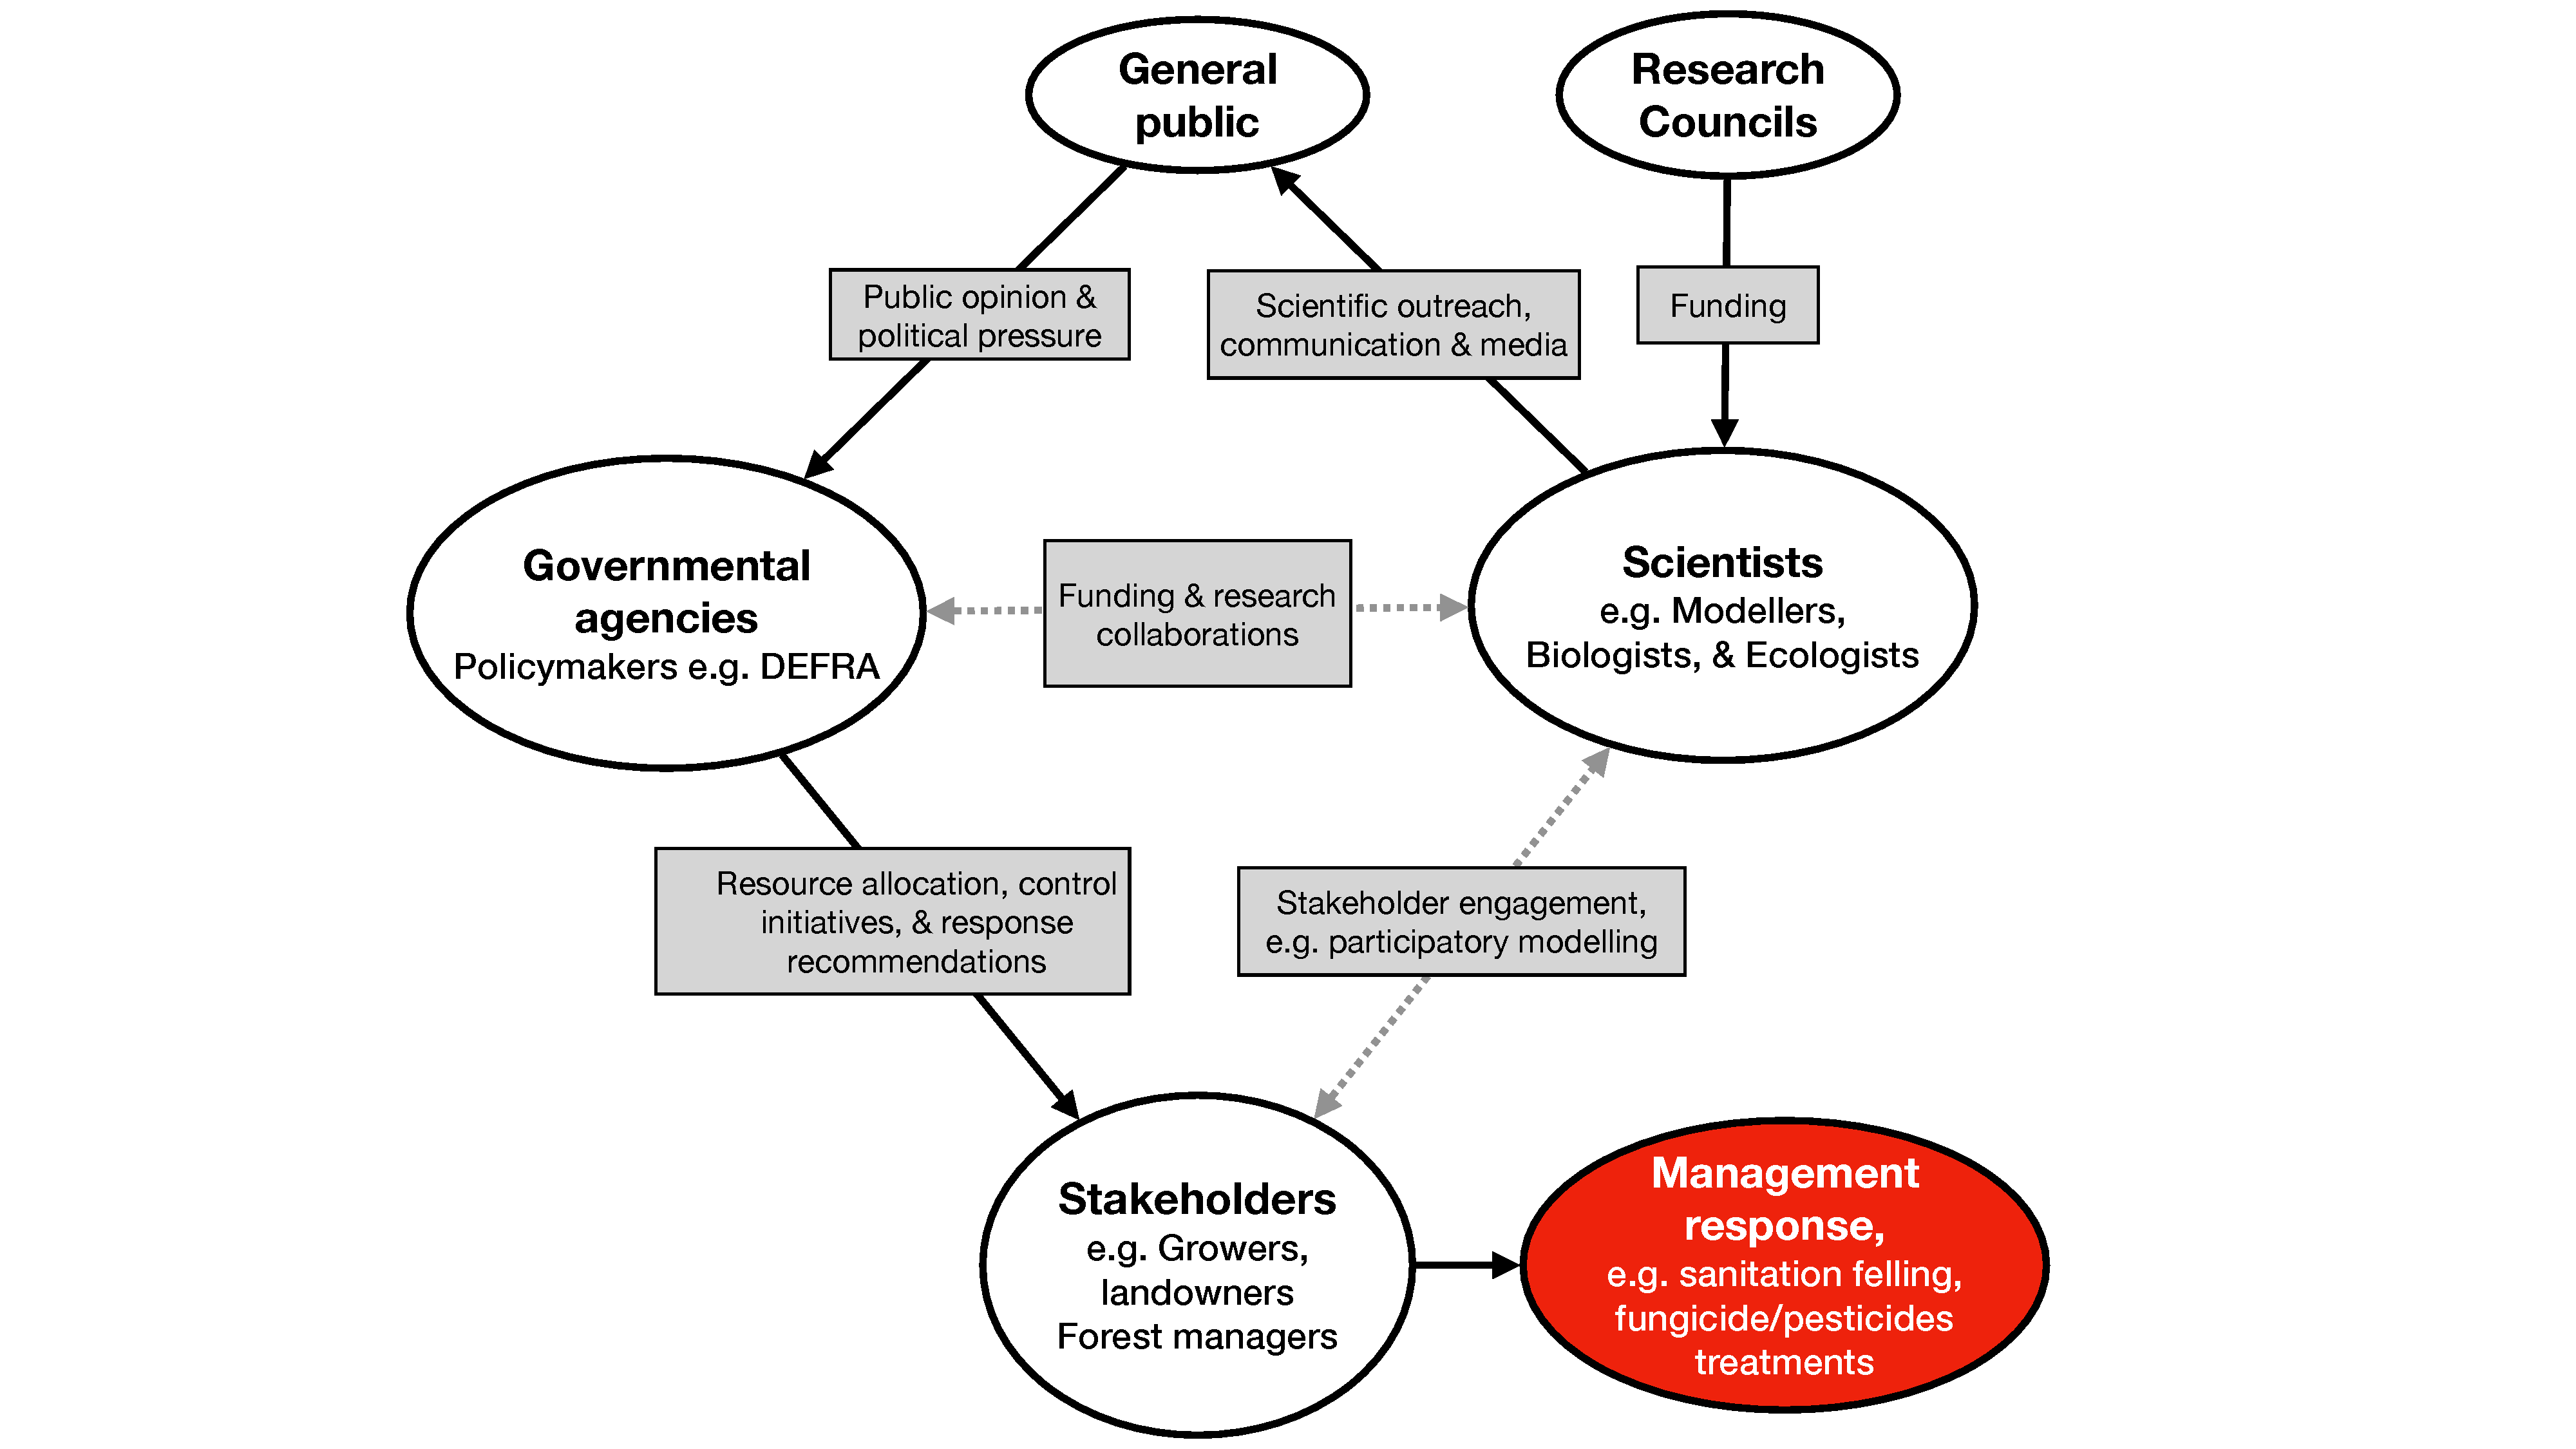
\includegraphics[scale=0.35]{chapter1/figures/modelling-and-policy.pdf}
    \caption{A simplified model representing the major socioeconomic interactions between the general public, scientists, policymakers and stakeholders in the UK. Scientists receive funding from and collaborate with Governmental bodies/policymakers. Policymakers make decisions and allocate resources to lead control initiatives to protect tree health. Affected stakeholders in the UK can choose to join voluntary control initiatives or be legally obliged to take action if served a statutory plant health notice. }
    \label{fig:modelling-and-policies}
\end{figure}

Alternatively, scientists can engage stakeholders directly (discussed more below) or influence public opinion through outreach and
scientific communication. In turn, the public can influence the decisions of policymakers by
mounting sufficient political pressure \cite{fuller2016public}.
Unfortunately, several obstacles inhibit a well-informed, timely and effective response. 
In particular, poor accessibility to scientific research is widely-known to inhibit policy adoption, 
primarily because disseminating scientific information requires in-depth domain knowledge and technical skill \cite{jones2020modelling}.
In a bid to make their work more accessible to policymakers and stakeholders, modellers have endeavoured to construct user-friendly interfaces\footnote{
The reader can find the user-friendly modelling interface constructed by \cite{WEBIDEMICS} at \nolinkurl{http://www.webidemics.com}} \cite{WEBIDEMICS}.
Other strategies to leverage scientific output involve directly facilitating discourse between modellers and stakeholders, categorised as `participatory modelling' (\acrshort{pm}).

Recently, PM has become popular in `risk and natural disaster' modelling research \cite{hamalainen2020leadership, ravera2020participatory, hedelin2017participatory}. Nonetheless, PM approaches are rare in the context of plant disease, as reviewed by \cite{gaydos2019forecasting}.
In addition to a literature review, \cite{gaydos2019forecasting} held an interactive workshop with stakeholders regarding the spread of \textit{P. ramorum} in the United States. The workshop facilitated stakeholder engagement with an epidemic model \cite{tonini2017tangible}\textemdash reviewed in Chapter \ref{chapter2:litreview}. In particular, the authors reported that the stakeholders engaged well with the model and confirmed that the results were broadly consistent with observations in the field. However, and most interestingly, stakeholders with expert knowledge of the landscape remained sceptical of the host distributions' accuracy and resolution. In particular, stakeholders with domain knowledge on the ground thought that these inaccuracies could influence spatial dynamics in the simulation. Such insights are hard to deduce for modellers who generally remain less connected to the actual landscape. As such, \cite{tonini2017tangible} demonstrated a positive motivation to facilitate the collaboration 
between plant-health modellers and stakeholders through PM.

An effective response generally relies on widespread adoption of policies among multiple stakeholders, which is thought to depend on several additional factors. As an example, \cite{milne2020makes} coupled an epidemic model of citrus huanglongbing disease (HLB) and stakeholder opinion dynamics. In the behaviour model, stakeholder
opinions depended on research, other citrus growers, consultants, and the media. The perception of risks and trust in area-wide control led the stakeholders to join an area-wide control initiative. Subsequently, the analysis of \cite{milne2020makes} suggests that the efficiency of epidemic control led to more stakeholder-engagement than the perceived risks, and that frequent contact between stakeholders and advisors increases the probability of successful control.
% In the UK, stakeholders can either join control initiatives on a voluntary basis, or for certain pathogens be required by law to remove infected trees 
% as noted by \cite{tomlinson2015managing} in reference to oak processionary moth in London.

\newpage

\section{Chapter summary}

In this thesis, our motivation is to develop robust epidemic models of infectious tree disease epidemics to predict epidemic severity over GB and help guide policymakers. Firstly, we begin with a simple two-parameter percolation, from which more realistic and elaborate dispersal models follow. 
In particular, previous large-scale investigations have focused on specific pathosystems in a dynamic metapopulation-like setting
\cite{large-scale-control, meentemeyer2011epidemiological, harwood2009epidemiological}. We take an alternative approach and develop a general-purpose framework to spatially scale up a small-scale epidemic model (between individual trees) over large areas. The result is an $R_0$-map across GB with closer parallels to the emerging field of Infectious Disease Cartography in human and livestock diseases \cite{otieno2021modeling, KRAEMER201619, messina2016mapping}.

Chapter \ref{chapter2:litreview} begins by outlining several requisite modelling themes. First, the review examines
several seminal works that founded the field of quantitative botanical epidemiology. Following this,
a suite of small, large and multi-scale spatial epidemic models are reviewed. Additionally,
the Chapter provides an account of host distribution datasets available in GB. Lastly, a case study of the emerging
ash dieback epidemic is presented.

Chapter \ref{chapter:SLM} sets the scene with a percolation-based simple lattice model (\acrshort{slm}) of tree
disease spreading through a dense forest \cite{OROZCOFUENTES201912}. The model is compartmentalised
into a susceptible-infected-removed (\acrshort{sir}) framework and demonstrates a sharp transition threshold above which an epidemic will propagate. 
Above the threshold of transition, a travelling wave-like behaviour is demonstrated.

Chapter \ref{chapter:SLM-applications} builds on the percolation model constructed in Chapter \ref{chapter:SLM}.
Firstly, we extend the work of \cite{OROZCOFUENTES201912} and present an alternative method to detect an early
warning signal in two-dimensional parameter space. Lastly, the epidemic model is coupled to a map of predicted
oak abundance over GB \cite{hill.data} to outline a large-scale `toy' model of tree disease. 
Primarily, Chapter \ref{chapter:SLM-applications} demonstrates that nearest-neighbour interactions are problematic
for realistic tree densities, which motivates an improved dispersal model. 

Chapter \ref{ch5:dispersal-model} introduces a generic Gaussian dispersal kernel into the epidemic model, denoted as the non-local model (\acrshort{nlm}). 
Ensuing epidemics in the NLM are demonstrated to spread at lower tree densities, frequent across GB, thereby overcoming the inherent nearest-neighbour limitations witnessed in Chapters \ref{chapter:SLM}-\ref{chapter:SLM-applications}.
Disease spread is then examined over a range of dispersal scale parameters and compared to the standard SIR model. Next, a spatially-explicit analytic expression for $R_0$ is derived and compared to a `\textit{contact tracing}' method of calculating $R_0$.
Both methods of determining the reproductive ratio are shown to demonstrate a threshold at $R_0=1$.

Chapter \ref{ch:6-adb} develops the dispersal model of Chapter \ref{ch5:dispersal-model} towards a mechanistic model reflecting the life cycle of ash dieback. The model involves susceptible-exposed-infected-removed (\acrshort{seir}) compartments that repeat annually according to the sexual reproduction of ash dieback. Consequently, a method is presented to compose $R_0$-maps
across GB using the map of predicted ash abundance given by \cite{hill.data}. Lastly, a connected-component-analysis
(\acrshort{cca}) algorithm is used to visualise  clustering and risk in the $R_0$-map. Examining the clustering as a function
of infectivity reveals behaviour akin to a global epidemic phase transition across the map. That is, below a certain infectivity threshold, 
the pathogen would not be able to invade GB.

Chapter \ref{ch7:landscape-level-control} proceeds from observations discussed in \ref{ch:6-adb}. 
Namely, Chapter \ref{ch7:landscape-level-control} presents the first steps toward a novel landscape-level
control strategy based on the large-scale host structure. More specifically, the epidemic control strategy targets
natural pinch-points and fault lines in the spatial distribution of hosts to bottleneck the epidemic
spread between at-risk regions. The Chapter ends by discussing the major assumptions in the control method and presents
a series of research questions that need to be addressed before the control method is demonstrated sufficiently.

Chapter 8 discusses the limitations and future developments of the work presented in this thesis.

% 2) A review of the `interdisciplinary' literature
\chapter{Interdisciplinary tree disease epidemics}
\label{chapter2:litreview} 

Understanding modern-day tree disease epidemics requires a holistic, interdisciplinary
approach, made possible only by the convergence of numerous scientific fields. 
Consequently, this Chapter reviews several key modelling themes.

Models of tree disease aim to help design effective control policies and inform policymakers.
Well-informed policymakers can then help to maintain tree health in rural, urban and commercial environments. 
Although myriad environmental, biological and anthropomorphic factors complicate the scientific understanding 
and thus effective disease control. 

Here, the review begins by narrating some early historical developments in human and botanical epidemiology before presenting
a variety of present-day modelling frameworks. After introducing the mainstream paradigm of plant-based epidemic models,
an inspection of dispersal, thresholds, and epidemic control follow naturally. Then, several tree distribution datasets in Great Britain are presented and compared. Finally, the Chapter ends with a case study of ash dieback, reflecting the multi-faceted 
difficulties posed by a recent emergent epidemic.

\section{Historical perspectives}

Historically, the fields of plant pathology and mathematical epidemiology existed in different spheres.
Plant pathology researchers furthered biological understanding of pathogen growth (e.g. \cite{doi:10.1146/annurev.py.01.090163.000245}), not predictive mathematical theories.
Although, pioneering discoveries in mathematical epidemiology permitted a more quantitative treatment of botanical diseases. 
In particular, the seminal $SIR$ model of \cite{kermack-model} 
provided a foundation to examine plant-based epidemics mathematically.

\subsection{Standard $SIR$}

The \cite{kermack-model} (K \& M) model involves three compartmentalised fields, 
susceptible $S(t)$, infected $I(t)$ and removed $R(t)$.
Each field models the evolution of a closed population of size $N$, where $N = S(t) + I(t) + R(t)$. 
A coupled system of ODEs then follow:
\begin{align}
\label{eq:SIR-model1}
    &\frac{dS}{dt} = -\beta SI \\
    &\frac{dI}{dt} = \beta SI - \mu I \\
    \label{eq:SIR-model3}
    &\frac{dR}{dt} = \mu I
\end{align}
where the term $\beta S I$ dictates the flow of susceptible hosts into the infected compartment according 
to the rate $\beta$. Likewise, $\mu I$ controls the transition of infected hosts into the removed compartment
through a removal rate $\mu$. Figure \ref{fig:SIR-vs-plank}(a) illustrates the coupled $SIR$ system for 
fixed $\mu$ and four values of $\beta$.

The coupled differential system of Equations (\ref{eq:SIR-model1}-\ref{eq:SIR-model3}) rely on several assumptions, including:
1) a closed population with no births or deaths 2) no exposed/incubation period 3) lifetime immunity following recovery
4) mass action population mixing, where contact mixing rates between individuals in $S$ and $I$ are proportional 
to the number of individuals in either field.

Today, countless articles have relaxed these assumptions to extend the standard $SIR$ framework\footnote{
Indeed, following the COVID-19 pandemic, $SIR$-type models remain an active field of research 
and dominate present-day epidemic literature \cite{atkeson2020using}.}.
Nevertheless, a keystone result emerged from Equations (\ref{eq:SIR-model1}-\ref{eq:SIR-model3}), namely 
the existence of a critical epidemic threshold, captured through either:
\begin{align}
    \label{eq:R0-SIR}
    & R_0 = \frac{\beta}{\mu}\\
    \label{eq:R0-effective}
    & R_e = \frac{S(t)}{N} \frac{\beta}{\mu}
\end{align}
where $R_0$ and $R_c$ are referred to as the basic and effective reproduction numbers, respectively.
Following the introduction of one infected host at $t=0$, $N\sim S(0)$ and 
we have $R_e=\big((N-1)/N\big) \beta / \mu$. Therefore, in the limit of a large population at $t=0$, 
$\big((N-1)/N\big)$ approximates unity and $R_e = R_0$, otherwise $R_e=\big(S(t)/N\big) R_0$.

Both quantities $R_0$ and $R_e$ describe an epidemic threshold, though $R_e$ captures a threshold in the face
of a declining susceptible population by including the ratio $S(t)/N$.
Equation \ref{eq:R0-effective} defines a critical threshold by the simple criterion\footnote{
For a more comprehensive mathematical proof of $SIR$
model thresholds, the reader is directed towards \cite{weiss2013sir}}:
1) when $R_e > 1$, then $I(t)$ rises sharply, culminating in an epidemic before declining in the absence of newly
infected hosts
2) if $R_e \leq 1$, then $I(t)$ quickly declines to zero as $t\rightarrow 0$ and the outbreak subsides.


\subsection{Logistic growth}

The seminal work of \cite{van2013plant} firmly established ties between plant pathology and 
mathematical epidemiology.
Fundamentally, Van der Plank equated the growth of plant pathogens (or `inoculum') to logistic growth of the form:
\begin{equation}
    \label{van-plank}
    \frac{dI}{dt} = rI(1 - I)
\end{equation}
where $r$ describes the rate of pathogen growth and $I$ reflects the proportion of infected tissue.
In Equation \ref{van-plank}, the amount of infected tissue $I$ snowballs at first, 
in proportion to the amount of inoculum. Then, as time passes and $I$ grows, $(1-I)$ approximates zero, 
and the system plateaus as all susceptible tissue becomes infected.
The essential model behaviour is shown in Figure \ref{fig:SIR-vs-plank}(b) over $10$ values growth rates $r$.
From Equation \ref{van-plank}, a simple method to determine the rate $r$ follows:
\begin{equation}
    \label{eq:van-plank-r}
    r =\frac{1}{t_2 - t_1} \log \Big(\frac{I_2}{1 - I_2} - \frac{I_1}{1 - I_1}\Big)
\end{equation}
where $I_1$ and $I_2$ are the proportions of infected tissue at times $t_1$ and $t_2$ respectively\textemdash 
see \cite{van2013plant} Chapter 3. Importantly, both $I_1$ and $I_2$, and by extension the infection rate $r$,
are measurable in laboratory conditions. 
In Equation \ref{van-plank}, newly infected tissue becomes infectious immediately following infection.
Realistically, infectious tissue (and symptom expression) takes time to develop, described by an `incubation period'.
Accordingly, Van der Plank adapted Equation \ref{van-plank} to a delay differential equation (DDE):
\begin{equation}
\label{van-plank-incubation}
    \frac{dI_t}{dt} = RI_{t-p}(1 - I_{t})
\end{equation}
where $I_t$ and $I_{t-p}$ describe the infectious tissue at times $t$ and $t-p$ and $p$ is the incubation period. 
Hence, infectious tissue grows in response to the factor $R I_{t-p}$, and saturates
according to the logistic term $(1 - I_t)$. The parameter $R$ now describes pathogen
growth at step $t-p$, as opposed to $r$ that describes the spread of disease at step $t$, leading to the ratio:
\begin{equation}
    \frac{R}{r} = \frac{x_t}{x_{t-p}}
\end{equation}
\begin{figure}
     \centering
     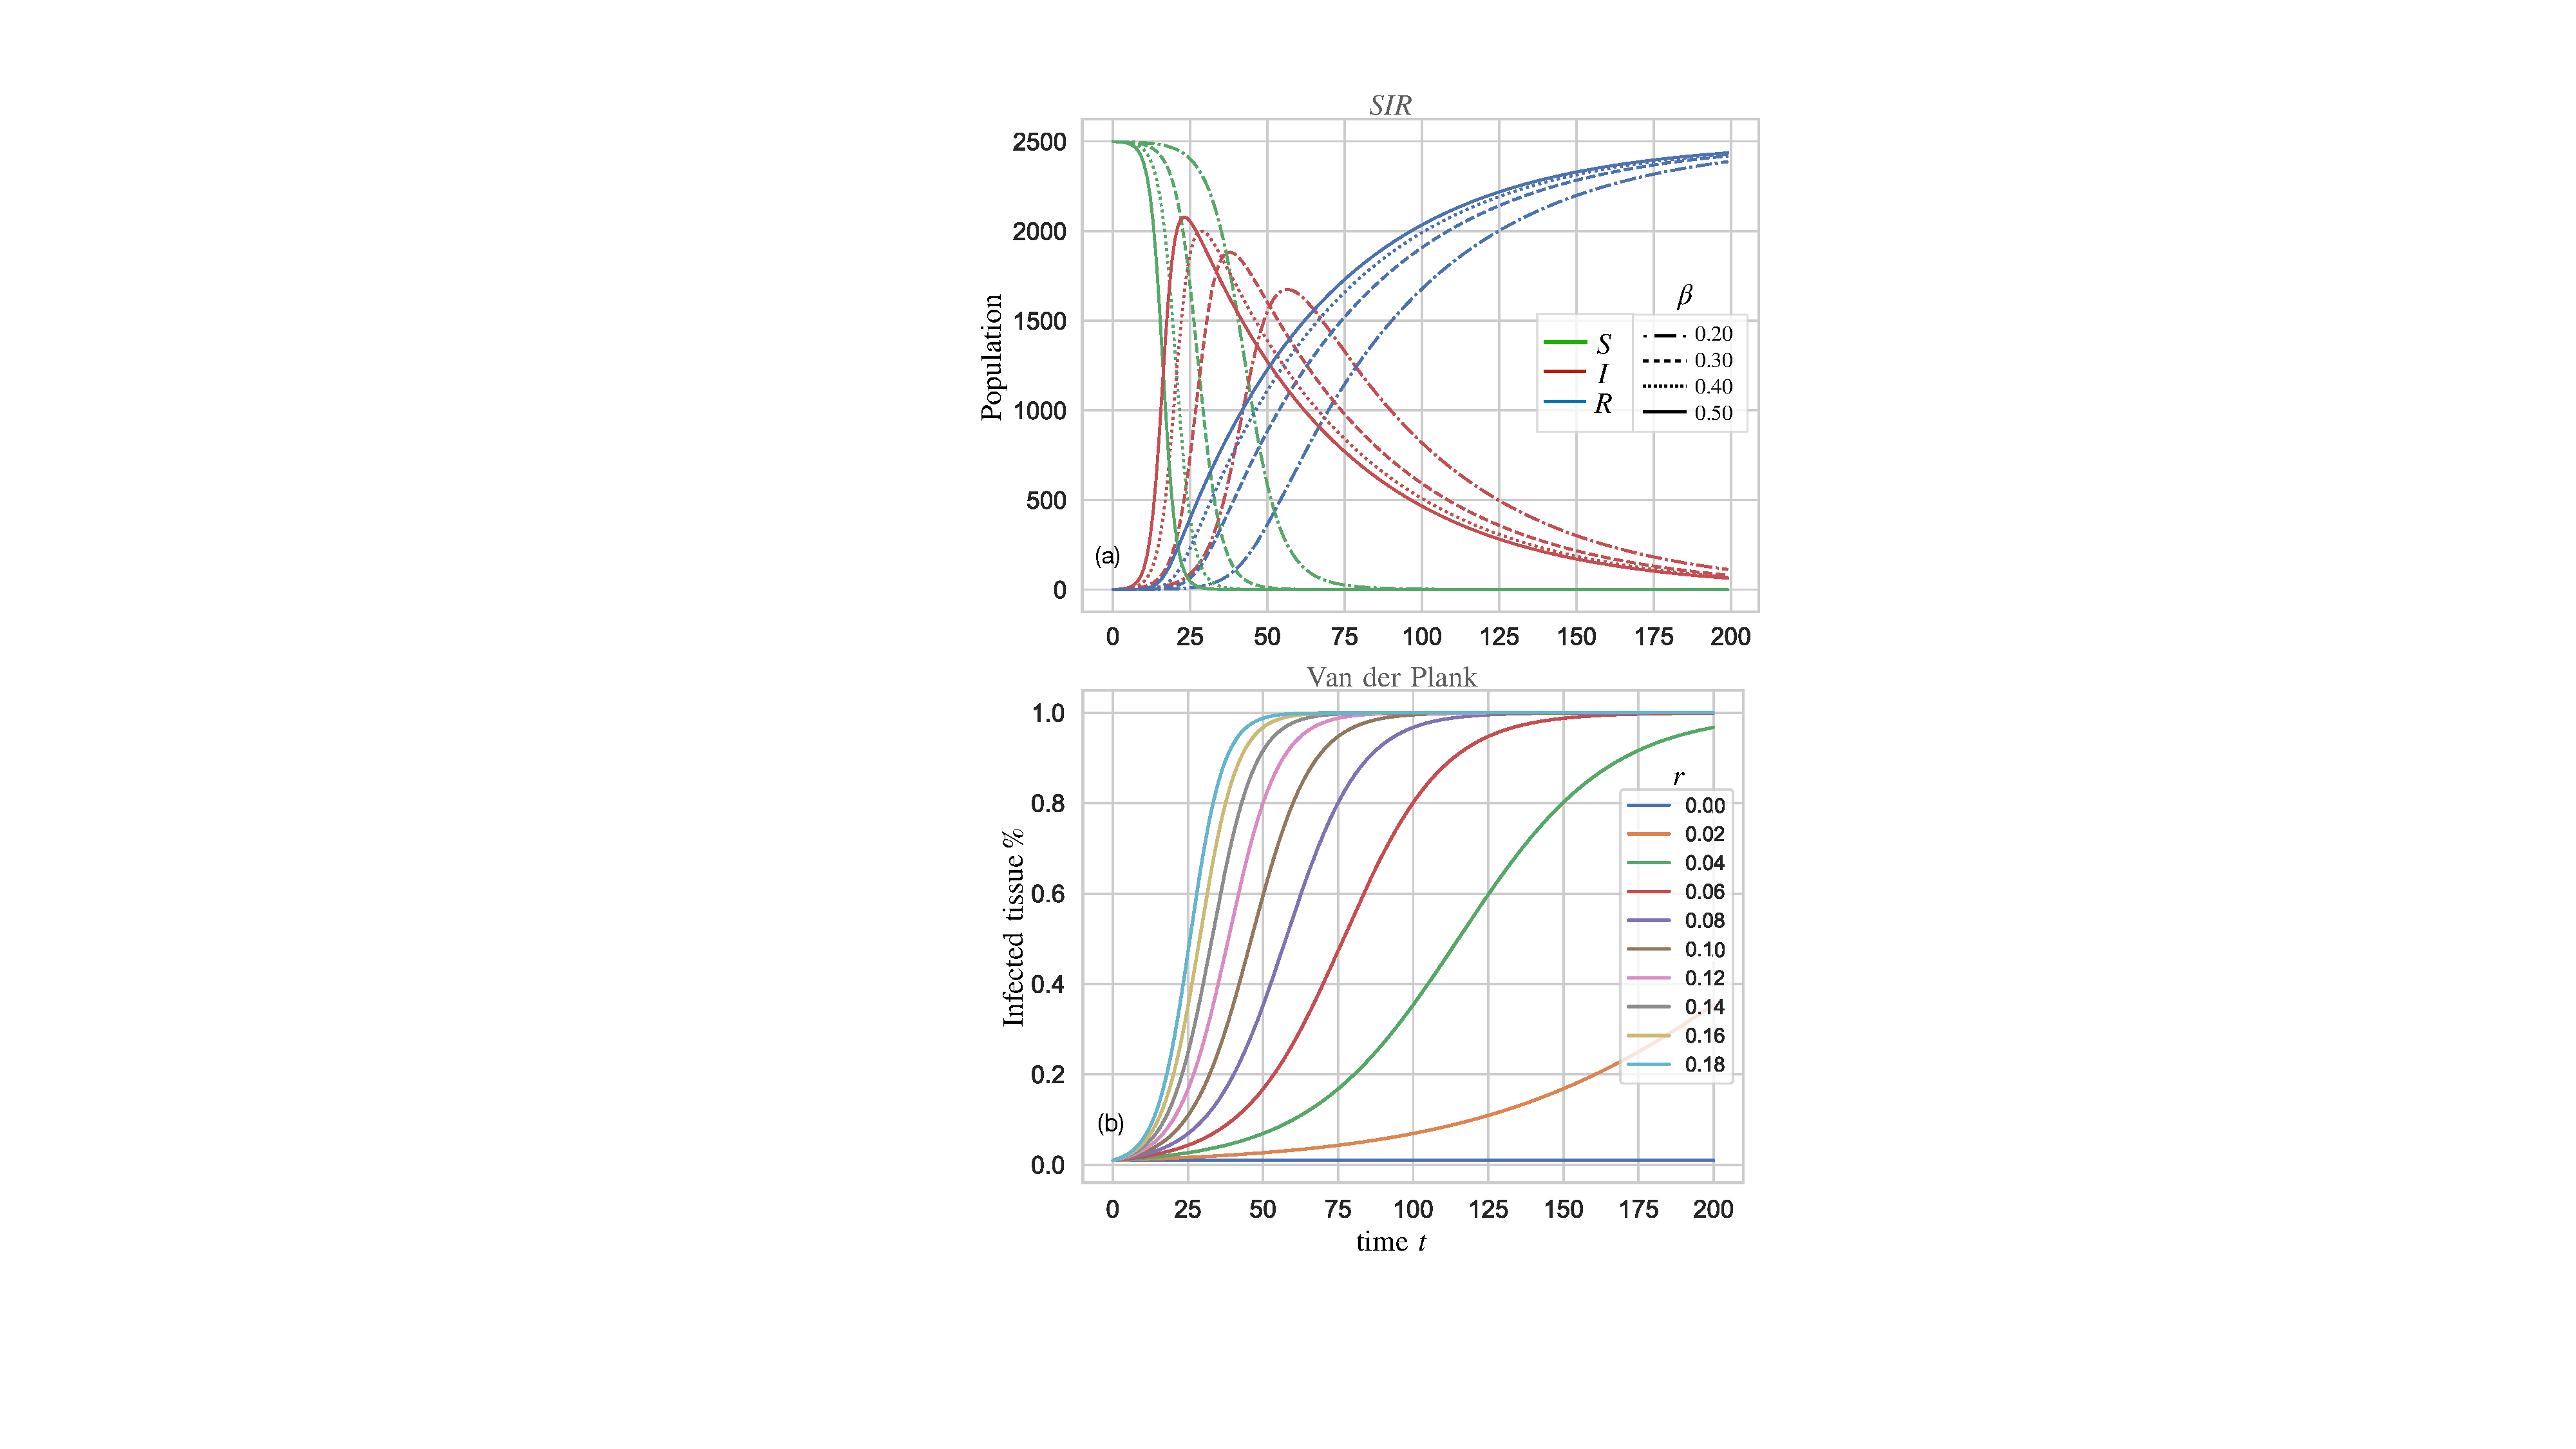
\includegraphics[scale=0.55]{chapter2/figures/SIR-vs-Plank.pdf}
     \caption{(a) The $SIR$ model as presented by \cite{kermack-model} is shown for fixed removal rate $\mu = 0.20$ and variations of $\beta$. 
                  The coupled system of ODEs can be solved numerically with Euler's method. Here, simulations begin with 
                  $2500$ susceptible and one infected individuals, and evolve for $t=200$ steps.
                  (b) The logistic growth model \cite{van2013plant} used to describe the growth of infected plant material.
                  Simulations are numerically computed with a forward-time finite difference method for $10$ different growth rates $r$.
       } 
     \label{fig:SIR-vs-plank}
 \end{figure}
where $r$ represents an `apparent' infection rate (measurable in laboratories from Equation \ref{eq:van-plank-r}),
and $R$ denotes the `basic' infection rate. As Plank explained, one usually seeks
to determine $R$ from the constant $r$. Assuming that $r$ indeed stays constant over the epidemic:
the basic infection rate $R$ must decrease as $x_t/x_{t-p}$ gets progressively smaller as $x_{t-p}\rightarrow x_t $.
At this point, the basic infection rate $R$ begins to resemble the effective reproduction ratio $R_e$
from Equation \ref{eq:R0-effective}. 

Equation \ref{van-plank-incubation} describes a system where
infections incubate for a period $p$ before inducing the growth of more infectious plant tissue.
However, it does not describe the infectious period (where infected tissue remains before becoming epidemiologically inert),
which lead Plank to extend Equation \ref{van-plank-incubation} to:
\begin{equation}
\label{van-plank-infectious-p}
    \frac{dI_t}{dt} = R_c(I_{t-p} - I_{t-i-p})(1 - I_{t})
\end{equation}
where $R_c$ is the basic infection rate `corrected' for removals and $i$ is the infectious period.
In this DDE, a unit of latently infectious tissue starts becoming infectious after $p$ steps, and stops becoming infectious $i$ steps.
More formally, as $I_{t-i-p} \rightarrow I_{t-p}$, the rate of infectious tissue growth approaches zero, $dI_t/dt \rightarrow 0$.

\subsection{Contrasting approaches}

The $SIR$ model does not include an incubation period, and therefore differs from the delayed differential formulation 
of Equation \ref{van-plank-infectious-p}. Nonetheless, the compartmentalised approach is easy to extend, leading to an 
$SEIR$ system:
\begin{align}
\label{eq:SEIR-model1}
    &\frac{dS}{dt} = -\beta SI \\
\label{eq:SEIR-model2}
    &\frac{dE}{dt} = \beta SI - \gamma E\\
    &\frac{dI}{dt} = \gamma E - \mu I \\
    \label{eq:SEIR-model3}
    &\frac{dR}{dt} = \mu I
\end{align}
where Equation \ref{eq:SEIR-model2} describes the population of latently (or exposed) infected hosts.
Susceptible hosts transition into the exposed compartment at the same rate as before, namely $\beta SI$, but now have an
exponentially distributed latency period of $\gamma^{-1}$ before transitioning into $I$.

Both Equations \ref{eq:SEIR-model1}-\ref{eq:SEIR-model3} and Equation \ref{van-plank-infectious-p} outline similar systems,
though infected tissue in Equation \ref{van-plank-infectious-p} remains infectious for precisely $i$ units.
This contrasts with the exponentially distributed exposed lifetime implicit within Equation \ref{eq:SEIR-model2}.
Nevertheless, \cite{segarra2001epidemic} illustrated how Plank's DDE and the $SEIR$ system are both special cases of
the $SIR$ model proposed by \cite{kermack-model}, when the $SIR$ model incorporates a sporulation function, $\phi(\tau)$. 
The sporulation function appropriately models spore production in plant pathogens. 
In particular, if $\phi(\tau) = 0$ for small $t$, $\phi(\tau)$ can model incubation periods. 
Similarly, if $\phi(\tau) = 0$  for large $t$, we recover an infectious period. 
More recently, \cite{time-varying-infectivity} simplified the analysis of \cite{segarra2001epidemic}, showing that 
both Plank's DDE and the $SEIR$ model can be recovered with an $SE_nI_mR$ model.
In an $SE_nI_mR$ framework, both $n$ and $m$ represent an arbitrary number of distinct exposed and infectious compartments:
\[
    S\rightarrow E_1 \rightarrow E_2 \rightarrow ... \rightarrow E_n \rightarrow I_1 \rightarrow I_2 \rightarrow ... I_m
\]
Trivially, the $SEIR$ model is recovered when $n=1$ and $m=1$. However, when $n,m \rightarrow \infty$,
\cite{time-varying-infectivity} demonstrated that we recover an expression equivalent to the DDE in Equation \ref{van-plank-infectious-p}.
Despite the sameness of both DDE and $SEIR$ formulations, the overarching theme of modern epidemiology is overwhelmingly compartmentalised,
owing to the increased flexibility and easier analysis of compartmental models.

\subsection{Progressive botanical epidemiology}
\label{sec:prog-epi}
After \cite{van2013plant} moved the field of botanical diseases into a more quantitative discipline,
theoretical investigations (alongside the adoption of computer simulations) characterised the next few decades.
Plank's DDE was applied to numerous pathosystems, halo blight in beans \cite{doi:10.1111/j.1744-7348.1979.tb06527.x} 
and grape powdery mildew \cite{sall1980epidemiology} to name a few. In particuar, \cite{sall1980epidemiology} adapted Plank's
logistic approach to include a time-varying infection rate $r(t)$. Moreover, diverse mathematical techniques, 
including multiple  regression analysis, were incorporated into mainstream plant epidemiology \cite{butt1974multiple}. 
Subsequently, \cite{zadoks1979epidemiology} consolidated various early mathematical models of plant disease 
alongside \cite{jeger1984use}.

Developments in computing compounded advances in plant epidemiology through this period. 
Improved accessibility and computer architectures permitted faster calculations and more intensive models. 
The first epidemic simulator (EPIDEM) written in FORTRAN IV came by \cite{waggoner1969epidem}. 
EPIDEM modelled the fungi `Alternaria solani' spreading through infected potato and tomato leaf tissue under different environmental conditions. 
    
An interesting early simulator (EPIMUL76) developed by \cite{zadoks1977role} adapted Van der Plank's logistic growth model into a spatio-temporal framework of two spatial dimensions. 
EPIMUL76 simulated the spread of disease on a two-dimensional domain, subdivided into $20\times 20$ host units referred to as `compartments', that took place inside a computer with $128\mathrm{K}$ of memory.
Arguably, subdividing the domain into separate compartments could be considered as an early agent-based model. 

In their analysis, \cite{zadoks1977role} alluded to the problem of scale in plant disease, as spatial scales
were conceptualised as `microscales' ($\leq 1\mathrm{m}$), `mesoscales' ($10^2\mathrm{m}$) and `macroscales' ($10^6\mathrm{m}$).
In this picture, microscales ranged from plant leaves to individual plants, mesoscales reflected crop fields, and macroscales
described large regional expanses over an entire country. Moreover, the probability of dispersal between infected hosts assumed a
Gaussian distribution\textemdash in contrast to \cite{doi:10.1146/annurev.py.06.090168.001201}.

In general, the ability to simulate more intricate models grew in proportion to the amount of computer memory available.
For a review of early plant disease simulators, see \cite{doi:10.1146/annurev.py.23.090185.002031}.

\subsection{Percolation: from forest fires to epidemics}
\label{section:lit-rev-perc}

Research on percolation occurred alongside the developing field of plant disease modelling.
The development of percolation theory marked an early approach to modelling epidemic systems that are
both spatially-explicit and stochastic.
The original formulation of percolation theory was first used to describe properties of a fluid and the 
bonds which form between molecules \cite{perco_origin} (a more formal account of 
percolation is undertaken in section \ref{ch3:invasions_and_persistence}). The problem was posed on a 
graph\textemdash illustrated in terms of vertices and edges. However re-interpretations were subsequently 
put forward by physicists studying material sciences, naturally on a lattice. \cite{Essam_1980}. 
The attractive feature of this new paradigm was that percolation demonstrated a phase-transition. 
Thus, percolation could be treated with scaling theory used in the study of critical-phenomena. 
Accordingly, early work rigorously ensued to map out the behaviour of percolation around criticality in 
terms of critical exponents \cite{STAUFFER19791}. 

Different flavours of percolation models, such as site or bond percolation, were described
to model different processes. Nevertheless, percolation proved a convenient theory and various phenomena including gelation, 
magnetism and telecommunications were described \cite{trove.nla.gov.au/work/26493727}. In particular, 
forest fire models were related to percolation \cite{MacKay_1984}, 
with only a short conceptual jump from time-dependent percolation used to study the growth of crystals \cite{Family_1985}. 

A fire spreading through a population of trees is not too different to a disease spreading through 
a population, thus leading to a general epidemic-formalisation within a percolation-based framework
\cite{pub.1059067807}; the researchers proposed that epidemics might be in the same universality class
as percolation. Beginning with a simple $SIR$ framework put forward by \cite{kermack-model}, the field 
of epidemiology was already well-established around the time percolation theory was conceived \cite{baily1975mathematical}. 
Naturally, percolation models could relax assumptions about population mixing and serve as a helpful tool
when developing spatially structured epidemic models.

A fractal-like pattern of epidemics was observed by \cite{GRASSBERGER1986273}, shown in Figure \ref{fig:1d_perc_basis}. 
In Figure \ref{fig:1d_perc_basis}, lighter grey sites represent removed individuals, 
black sites indicate actively infected sites, and white sites indicate unaffected sites. 
All lattice sites in the bottom row were initially infected, and the infection can be seen to propagate
from the bottom up. The lattice was initialised at the critical-density $p\sim p_c$ culminating in a fractal-like pattern.
\cite{GRASSBERGER1986273} did not attribute the hosts of this model to be trees, but instead a general host-population with low mobility. 
The authors noted that local interactions between hosts and infected were vast simplifications and proposed 
generalising the system with long-range interactions following a power law. 
Although, it must be remarked that including long-range interactions would cease to describe a percolation based system.

\begin{figure}
    \centering
    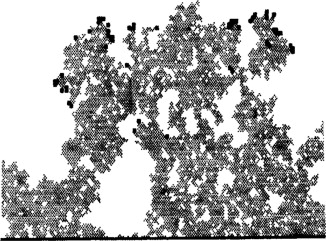
\includegraphics{chapter2/figures/perc1.jpg}
    \caption{A space-time representation of an epidemic spreading at the critical threshold. 
    The spatial (horizontal) and time (vertical) axis show self-similar propagation of diseased 
    individuals in grey, produced by \cite{GRASSBERGER1986273}}
    \label{fig:1d_perc_basis}
\end{figure}

Percolation models of epidemics were investigated by several means, 
e.g. renormalisation-groups \cite{pub.1060474189} and Monte-Carlo methods \cite{pub.1059069981}. 
Studies generally focused on finding the systems critical exponents and categorising phase
transition graph that characterised an epidemic (super-critical) or extinction (sub-critical) 
regimes \cite{GRASSBERGER1986273}. The properties of both epidemics and forest fire percolation 
models were studied together in \cite{pub.1052857560}, highlighting their similarity.
One of the first ecological applications was put forward by \cite{pub.1031591030}, 
who studied the effects of landscape distributions and percolation models 
(reflecting both forest fire and epidemics). In their study, \cite{pub.1031591030} 
combined $SIR$-like mechanics inside a percolation-based distribution of hosts and subsequently 
found a narrow regime where disease epidemics would spread, thus mirroring the threshold-like 
behaviour witnessed in the $SIR$ model. Although, here, the authors considered the possibility of host recovery.
% \textemdash \cite{GRASSBERGER1983157} <- reference for early considerations towards percolation as a model for tree diseases and percolation
% \textemdash \cite{SANDER2002293}, read and get more info + research links
\newpage

\section{Spatially-explicit epidemic models}
\label{ch2:lit-rev-compartmentalised-models}

Emergent infectious diseases (EIDs) in tree populations are multi-scale,
they can span regional, country or continental spatial scales. Considerable variations in landscape composition,
tree densities, population aggregation, and the climatic factors give rise to diverse spatio-temporal
patterns of disease spread \cite{he2019integrating, suzuki2003spatial}. Incorporating spatial structure
in tree-disease models is therefore vital to accurately capture the environmental influences upon host-pathogen 
interactions and dispersal \cite{liu2007characterizing}. This section outlines several approaches to modelling
the spread of tree disease.

\subsection{Small-scale: stochastic dispersal}
\label{ch2:dispersal}

Pathogen dispersal through wind, watercourse or human trade underpins a key feature of EDIs. 
Numerous functions have been used to model dispersal, but generally, all describe a continuous 
non-negative (real-valued) function that is normalisable: $\int_{-\infty}^{\infty}  D(x)dx = 1$.
Various review articles provide comprehensive functional examples \cite{bullock2017synthesis, nathan2012dispersal, howe1982ecology}; 
however, the general class of dispersal kernels include thin-tailed Gaussian and 
exponential alongside fat-tailed inverse power law variants.

Early plant disease simulators (e.g. EPIDEM and EPIMUL76) included stochastic dispersal\textemdash 
discussed at length in section \ref{sec:prog-epi}. A more recent article by \cite{parnell2010effect} 
modelled stochastic dispersal in Citrus canker to investigate the effects of landscape aggregation 
patterns and disease progression.
\cite{parnell2010effect} studied landscape patterns of two kinds: 
1) varying degrees of randomly distributed densities 
2) varying degrees of host aggregation.
The epidemic model was based on a series of prior Citrus canker works
\cite{parnell2009optimal, gilligan2008epidemiological, cook2008constructing}.
The epidemic model is described by:
\begin{equation}
\label{eq:prob-trans}
    Pr(S_i \rightarrow I_i)_{\Delta t} = 1 - \exp\big[- \beta \sum_j^N\exp^{-\alpha d_{ij}} + \epsilon \big]
\end{equation}
Here, a transition probability describes the $i^{th}$ susceptible tree becoming infected 
during the step $t \rightarrow t + \Delta t$ on account of $N$ infected trees.
Equation \ref{eq:prob-trans} assumes that dispersal exponentially decreases with distance (i.e. $\exp^{-\alpha d_{ij}}$), 
where $\alpha$ denotes the dispersal scale parameter. Infection pressure from the $j^{th}$ infected tree is multiplied by an
infection rate, $\beta$. The last parameter to consider in Equation \ref{eq:prob-trans}
is the primary infection rate $\epsilon$. The primary infection rate reflects the chance of infection from sources outside
the immediate system, i.e. at time $t=0$, distant infected populations external to the
closed host population under consideration.

The outside exponential term of Equation \ref{eq:prob-trans} depicts a cumulative exponential threshold above which 
trees become infected. Interestingly, this threshold is based on the `Skelle construction' \cite{sellke1983asymptotic}. 
More specifically, Skelle assumed that susceptive hosts need an arbitrary (cumulative) degree of infection
exposure before becoming infectious. Using Equation \ref{eq:prob-trans}, \cite{parnell2010effect} proceeded to define 
a control radius and found that both landscape aggregation and (randomly distributed) high host densities increase the
optimal control radius. 

A later paper by \cite{WEBIDEMICS} proceeded to generalise the Citrus canker model.
Primarily, the authors examined an $SECIR$ model\footnote{
Here, compartments are (S)usceptible, (E)xposed, (C)ryptic and (R)emoved) where $C$ 
denotes unobservable cryptic infections.}, though several other model variants were included. 
\cite{WEBIDEMICS} contrasted both Gaussian and Cauchy dispersal kernels.
Cunniffe et al. included dispersal parameters provided by \cite{neri2014bayesian}, who
assessed Cauchy kernels\textemdash in addition to exponential kernels.
The general model followed:
\begin{equation}
\label{eq: webidemics}
     \phi_i(t) = w(t)\big[\beta \sum_j K(d_{ij}; \alpha) + \epsilon \big]
\end{equation}
where $w(t)$ is a time-dependent infectivity function, $\epsilon$ is the primary infection 
(set to zero in the manuscript), $\beta$ is the rate of secondary infection, and $K(d_{ij}; \alpha)$
is the dispersal function. This time, Equation \ref{eq: webidemics} presents a rate of transition for a single
susceptible tree (from $S_i \rightarrow E_i$) under the influence of all infected neighbours (represented by the $j^{th}$ index),
as opposed to the probability of Equation \ref{eq:prob-trans}.

Cunniffe et al. examined the effects of a cull radius, similar to \cite{parnell2010effect}. 
However, this time, results were aimed towards assessing control when there is epidemic uncertainty.
Consequently, \cite{WEBIDEMICS} assessed different epidemic serveries by varying $\beta$, alongside
numerous control parameters, e.g. eradication response time, detection probabilities and revisit/survey intervals. 

All in all, \cite{WEBIDEMICS} highlighted an intuitive result, namely, that the scale of control should
reflect the "intrinsic epidemic scale". More succinctly, \textit{aggressive pathogens should be met with 
an aggressive control strategy}. Moreover, Cunniffe et al. suggested that thick-tailed dispersal kernels
(in this case, a Cauchy distribution) prove more challenging to control.

The Citrus canker models developed in Equations \ref{eq:prob-trans} and \ref{eq: webidemics} 
contrast with non-spatial analytical systems. For example, the model of pine wilt disease (PWD)
constructed by \cite{khan2020modelling}, who coupled a differential system of pine (H)osts and beetle (V)ectors 
following:
\begin{align}
    \label{eq:PWD-model1}
    &\frac{dS_H}{dt} = \lambda_H - \beta_1\Psi S_H I_V - \beta_2\Phi\alpha S_H I_V - \gamma_1 S_H \\
    &\frac{dE_H}{dt} = \beta_1\Psi S_H I_V - \beta_2\Phi\alpha S_H I_V  - (\gamma_1 + m)E_H \\
    &\frac{dA_H}{dt} = m(1 - \omega)E_H - \gamma_1 A_H \\
    \label{eq:PWD-model-H}
    &\frac{dI_H}{dt} = m \omega E_H - (\gamma_1 + \mu ) I_H \\
    \label{eq:PWD-model-V}
    &\frac{dS_v}{dt} = \lambda_V - K S_v I_H - \gamma_2 S_V \\
    &\frac{dE_v}{dt} = K S_v I_H - (\gamma_2 + \eta) E_V \\
    \label{eq:PWD-model7}
    &\frac{dI_v}{dt} = \eta E_V - \gamma_2 I_V
\end{align}
In this system, pine tree hosts interact with beetle vectors that carry pathogenic nematodes 
(\textit{Bursaphelenchus xylophilus}). Stepping through the system:
Equations \ref{eq:PWD-model1}-\ref{eq:PWD-model-H} describe the host population;
births and naturally occurring deaths in the host population occur at rates $\lambda_H$ and $\gamma$, 
respectively. Pine trees become infected by two mechanisms: $\beta_1\Psi$ that describes the incidence
rate with infected mature beetles, and $\beta_2\Phi$ that describes the incidence rate with beetle offspring.
Once pine hosts become exposed, a fraction ($\omega$) transition into the infectious symptomatic state $I$, 
while the remaining fraction ($1 -\omega$) become asymptomatic\textemdash both pathways occur at rate $m$. 
Disease induced death happens at a rate $\mu$. Equations \ref{eq:PWD-model-V}-\ref{eq:PWD-model7} outline a 
($SEI$) dynamic for beetle vectors. Natural births and deaths in the beetle population happen with rates 
$\lambda_V$ and $\gamma_2$, respectively. Furthermore, susceptible beetles become exposed by feeding infected
hosts at rate $K$ and transitioning into the infected beetle class at rate $\eta$.

Equations \ref{eq:PWD-model1}-\ref{eq:PWD-model-H} assume mass action population mixing of beetles 
without stochasticity. Presumably, this assumption led \cite{khan2020modelling} to model PWD as a non-spatial
system on account of the migratory population of Beetle vectors. In reality, a dispersal kernel is likely to 
describe beetle movements more accurately than the well-mixed system presented in Equations 
\ref{eq:PWD-model1}-\ref{eq:PWD-model-H}. Case in point, the spatio-temporal dynamics of Asian longhorned
beetle was examined by \cite{smith2004dispersal} who inferred a median dispersal rate of $30\mathrm{m/day}$
according to an exponential dispersal kernel (with only $2\%$ of beetles exceeding $920\mathrm{m}$).
Linear stability analysis was performed on the deterministic system of Equations \ref{eq:PWD-model1}-\ref{eq:PWD-model-H}. 
Whereas the stochastic spatio-temporal framework of Equations \ref{eq:prob-trans} and \ref{eq: webidemics} 
were analysed by repeating simulations inside an ensemble.

% \begin{itemize}
%     \item The importance of dispersal
%     \item How is dispersal treated mathematically ?
%     \item What type of dispersal kernels have been studied?
%     \item What parameter-values have been inferred ?
%     \item How long-range can dispersal be ? Talk about long-range inter-Continental dispersal
%     \item see \cite{nathan2012dispersal} for a review of dispersal kernels
% \end{itemize}


\subsection{Large-scale}
% -\cite{doi:10.1098/rstb.1986.0072}
% -item \cite{large-scale-control}

Ultimately, microscopic (host-pathogen) interactions propagate the spread of disease. 
Although once disease-establishment has taken place, large-scale outbreaks can spread through vast
areas, e.g. the spread of ash dieback through Europe \cite{alsop2015ash}.
As a result, contemporary modes of tree disease have examined the large-scale spread over entire landscapes.
The previous section outlined some small-scale models (on the order of $1 \sim 10 \mathrm{km}$), 
however, in this section, we focus on large-scale epidemic models.

Over large scales, disease drivers include long distance dispersal (LDD) through wind \cite{golan2017long, gross2014h} and
trade \cite{ash-dieback-costs, perrings2016options, harwood2009epidemiological, doi:10.1098/rsif.2005.0051}.
However, linking human trade networks and dispersal in one large-scale model is challenging due to numerous complex parameters 
and epidemiological drivers. 

A framework constructed by \cite{harwood2009epidemiological} incorporated the growth and reproduction, dispersal and trade
of infectious plant material into a single model. The study conducted by \cite{harwood2009epidemiological} aimed
to assess the risk of \textit{Phytophthora ramorum} and \textit{Phytophthora kernoviae} in the UK by
employing a linked network approach. 
In the linked network, single grid cells of area $\mathrm{1km \times 1km}$ were coupled together by a (wind-borne)
dispersal kernel and a trade network. 
Following earlier earlier work \cite{madden2007study}, the population inside each grid cell evolved according
to an $SEIS$ model:
\begin{align}
    \label{eq:phyt-model1}
    &\frac{dS}{dt} = \mu E + \mu I - \beta S i\\
    &\frac{dE}{dt} =  \beta S i - k E - \mu E   \\
    \label{eq:phyt-model3}
    &\frac{dI}{dt} = k E - \mu I
\end{align}
where host introductions were assumed to balance the total number of removals $\mu (S + E + I$).
Then, dispersal between $\mathrm{1km \times 1km}$ grids took place inside a domain of size $\mathrm{700km \times 1300km}$ 
covering the UK. Here, the host population was informed by the Country side survey data\textemdash discussed more 
below in section \ref{ch2:hostdata}. An inverse square power law described wind-borne dispersal (with a scale constant
of $2\mathrm{m}$), though parameterisation was qualitative and uniformed by experimental data.

In addition, a simulated trade network linked $\mathrm{1km \times 1km}$ cells. 
In the trade network, plant nurseries and retailers were connected by LDD trade and transport. 
In this manner, \textit{Phytophthora ramorum} and \textit{Phytophthora kernoviae} could jump 
between cells. The same linked-network approach was later used to reconstruct the highly 
popularised 1970s Dutch elm disease epidemic in Great Britain \cite{doi:10.1111/j.1365-3059.2010.02391.x, potter2011learning}.

A similar construction was put forward by \cite{meentemeyer2011epidemiological} to 
forecast the spread of sudden oak death (SOD) in California from (1990-2030).
A distribution of host\footnote{In this context, `host' refers to a wide-range
species susceptible to \textit{P. ramorum} \cite{tooley2004susceptibility}.
} abundance was derived from previous SOD modelling work 
\cite{meentemeyer2004mapping} and comprised $\mathrm{250 \times 250}$ grid cells
weighted by the relative susceptibility to \textit{P. ramorum} from 1-100. As a result,
a high-resolution map of `host index' was produced throughout the state of California.

The large-scale SOD model included several epidemiological drivers of \textit{P. ramorum}: 
forest-type, local weather conditions, oak density, local pathogen growth and transmission
and longer-range transmission. Local-scale dispersal were estimated
using Markov chain Monte Carlo (MCMC) methods from aerial surveys \cite{valachovic2008wildland} 
of \textit{P. ramorum}, and positive sites (2001–2007) confirmed by the California Department of
Food and Agriculture were used to estimate the long-range dispersal. \cite{meentemeyer2004mapping}
found that a long-range Cauchy distribution fitted the data most appropriately over both spatial scales.
Hence, a multi-scale kernel was given as:
\begin{equation}
\label{eq:multi-scale-kernel}
    K(d; \alpha_1, \alpha_2, \gamma) = \gamma( 1 + (d/\alpha_1)^2 )^{-1} + (1 - \gamma)( 1 + (d/\alpha_2)^2 )^{-1}
\end{equation}
where $\alpha_1 = 20.57\mathrm{m}$ and $\alpha_2 = 9.5\mathrm{km}$ represent the short and long range dispersal
kernels respectively, and the ratio $\gamma=0.99$ estimates the total contribution to short and
long-range dispersal. Using the multi-scale dispersal kernel in Equation \ref{eq:multi-scale-kernel},
the epidemiological model between $\mathrm{250 \times 250}$ grid cells assume the form:
\begin{equation}
\label{eq:large-scale-model}
    \Psi_{ijt} = \beta \sum_i \big(\chi_t (f_i) m_{it} c_{it} I_{it} \big) \big( \chi_t(f_j) m_{jt} c_{jt} S_{jt} /N_{max} \big) \times K(d_{ij}; \alpha_1, \alpha_2, \gamma)
\end{equation}
where $\Psi_{ijt}$ represents the infection pressure from grid $i$ to grid $j$ in one week $t$ intervals. 
Equation \ref{eq:large-scale-model} includes multiple component-functions and parameters: 
\begin{itemize}
    \item A binary-valued function $\chi_t(f_i)$ that indicates if forest type $f_i$ can infect and become infected at time $t$
    \item two indices $m_{it}$ and $c_{it}$ that indicate moister and temperate of patch $i$ at time $t$
    \item $I_i$ and $S_j$, the number of infected in grid $i$ and susceptibles at $j$
    \item $K(d_{ij})$, the dispersal kernel from Equation \ref{eq:multi-scale-kernel}
    \item $\beta$ that models the rate of spore production per site per week.
\end{itemize}

From the model, \cite{meentemeyer2004mapping} predicted which areas in California
had the highest secondary infection risk of SOD over $40$ years.
Simulations were ensemble-averaged based on predicted weather conditions from 2008–2030.
Climatic variations were classified as `favourable', `random' and `unfavourable'.
In all variations, SOD was predicted to spread through California and effect $1000$s
of square kilometers. However, considerable spatial and temporal variation were witnessed
across different Californian states. Additionally, \cite{meentemeyer2004mapping} 
observed that $93\%$ of short-range dispersal occurred within the range of a single $\mathrm{250 \times 250}$ and 
$95\%$ of infrequent long-range spread remain within $100\mathrm{km}$ in their model.
Although, most dispersal remained localised $<1\mathrm{km}$.

The manuscript authored by \cite{meentemeyer2004mapping} emphasises the multi-faceted 
parameters and processes that one needs to consider before modelling a large-scale epidemic
outbreak; these included, host data, dispersal, and climate.
\cite{large-scale-control} subsequently extended the analysis of \cite{meentemeyer2004mapping}
to assess the large-scale effects of epidemic control. 
In particular, \cite{large-scale-control} examined how to optimise eradication of SOD with 
limited resources. When resources are low, the authors suggested that small localised 
eradication zones around \textit{known} foci optimise control; justified by the fact that
small, but more numerous, control areas about diseased areas reduces the risk of failing 
to treat a high-risk site that causes many secondary infections. 

\cite{large-scale-control} also tested management strategies based on targeting:
1) hosts irrespective of disease 
status (the "host" strategy)
2) local areas with high prevalence ("hazard" strategy)
3) areas with high basic reproduction numbers ("susceptible" strategy)
4) regions ahead of the wavefront ('wavefront" strategy).
Of all the management scenarios tested, \cite{large-scale-control} found
that 4), treating areas ahead of the wavefront, reduced epidemic spread the most.
In this scenario, the affected area was reduced by $\sim 2400\mathrm{km^2}$ and 
the optimal culling radius was determined to be $362.5\mathrm{m}$.

All the large-scale models discussed above split the population into smaller (sub)girds.
As such, they share noticeable similarities to a metapopulation\footnote{
Metapopulation dynamics generally aim to deconstruct a spatial population into separate sub-populations contained within a `patch'. Then, between-patch interactions aim to model population migrations, connectedness and fragmentation, while within-patch
dynamics aims to model colonisation, persistence, competition, coexistence, and habitat suitability.} commonly used by ecologists studying spatially-structured animal and plant populations \cite{hanski1998metapopulation}. 
However, plant-disease modellers increasingly utilise metapopulation settings to study the effects of landscape features on disease progression, e.g. \cite{beninca2020trade, soubeyrand2009spatiotemporal, doi:10.1046/j.1461-0248.2002.00378.x}.
 
% WORK IN PROGRESS
%     \item  \cite{https://doi.org/10.1111/jbi.13642}
%     \item  \cite{pautasso2013european}, search for 'modelling' in this review paper. It contains references to LDD models.
%     \item LDD is an important factor of the scale of spread. Long distance dispersal has been considered for many biological processesd distance between patches can...


\subsection{Disease fronts}

\blindtext

\blindtext

\begin{figure}
    \centering
    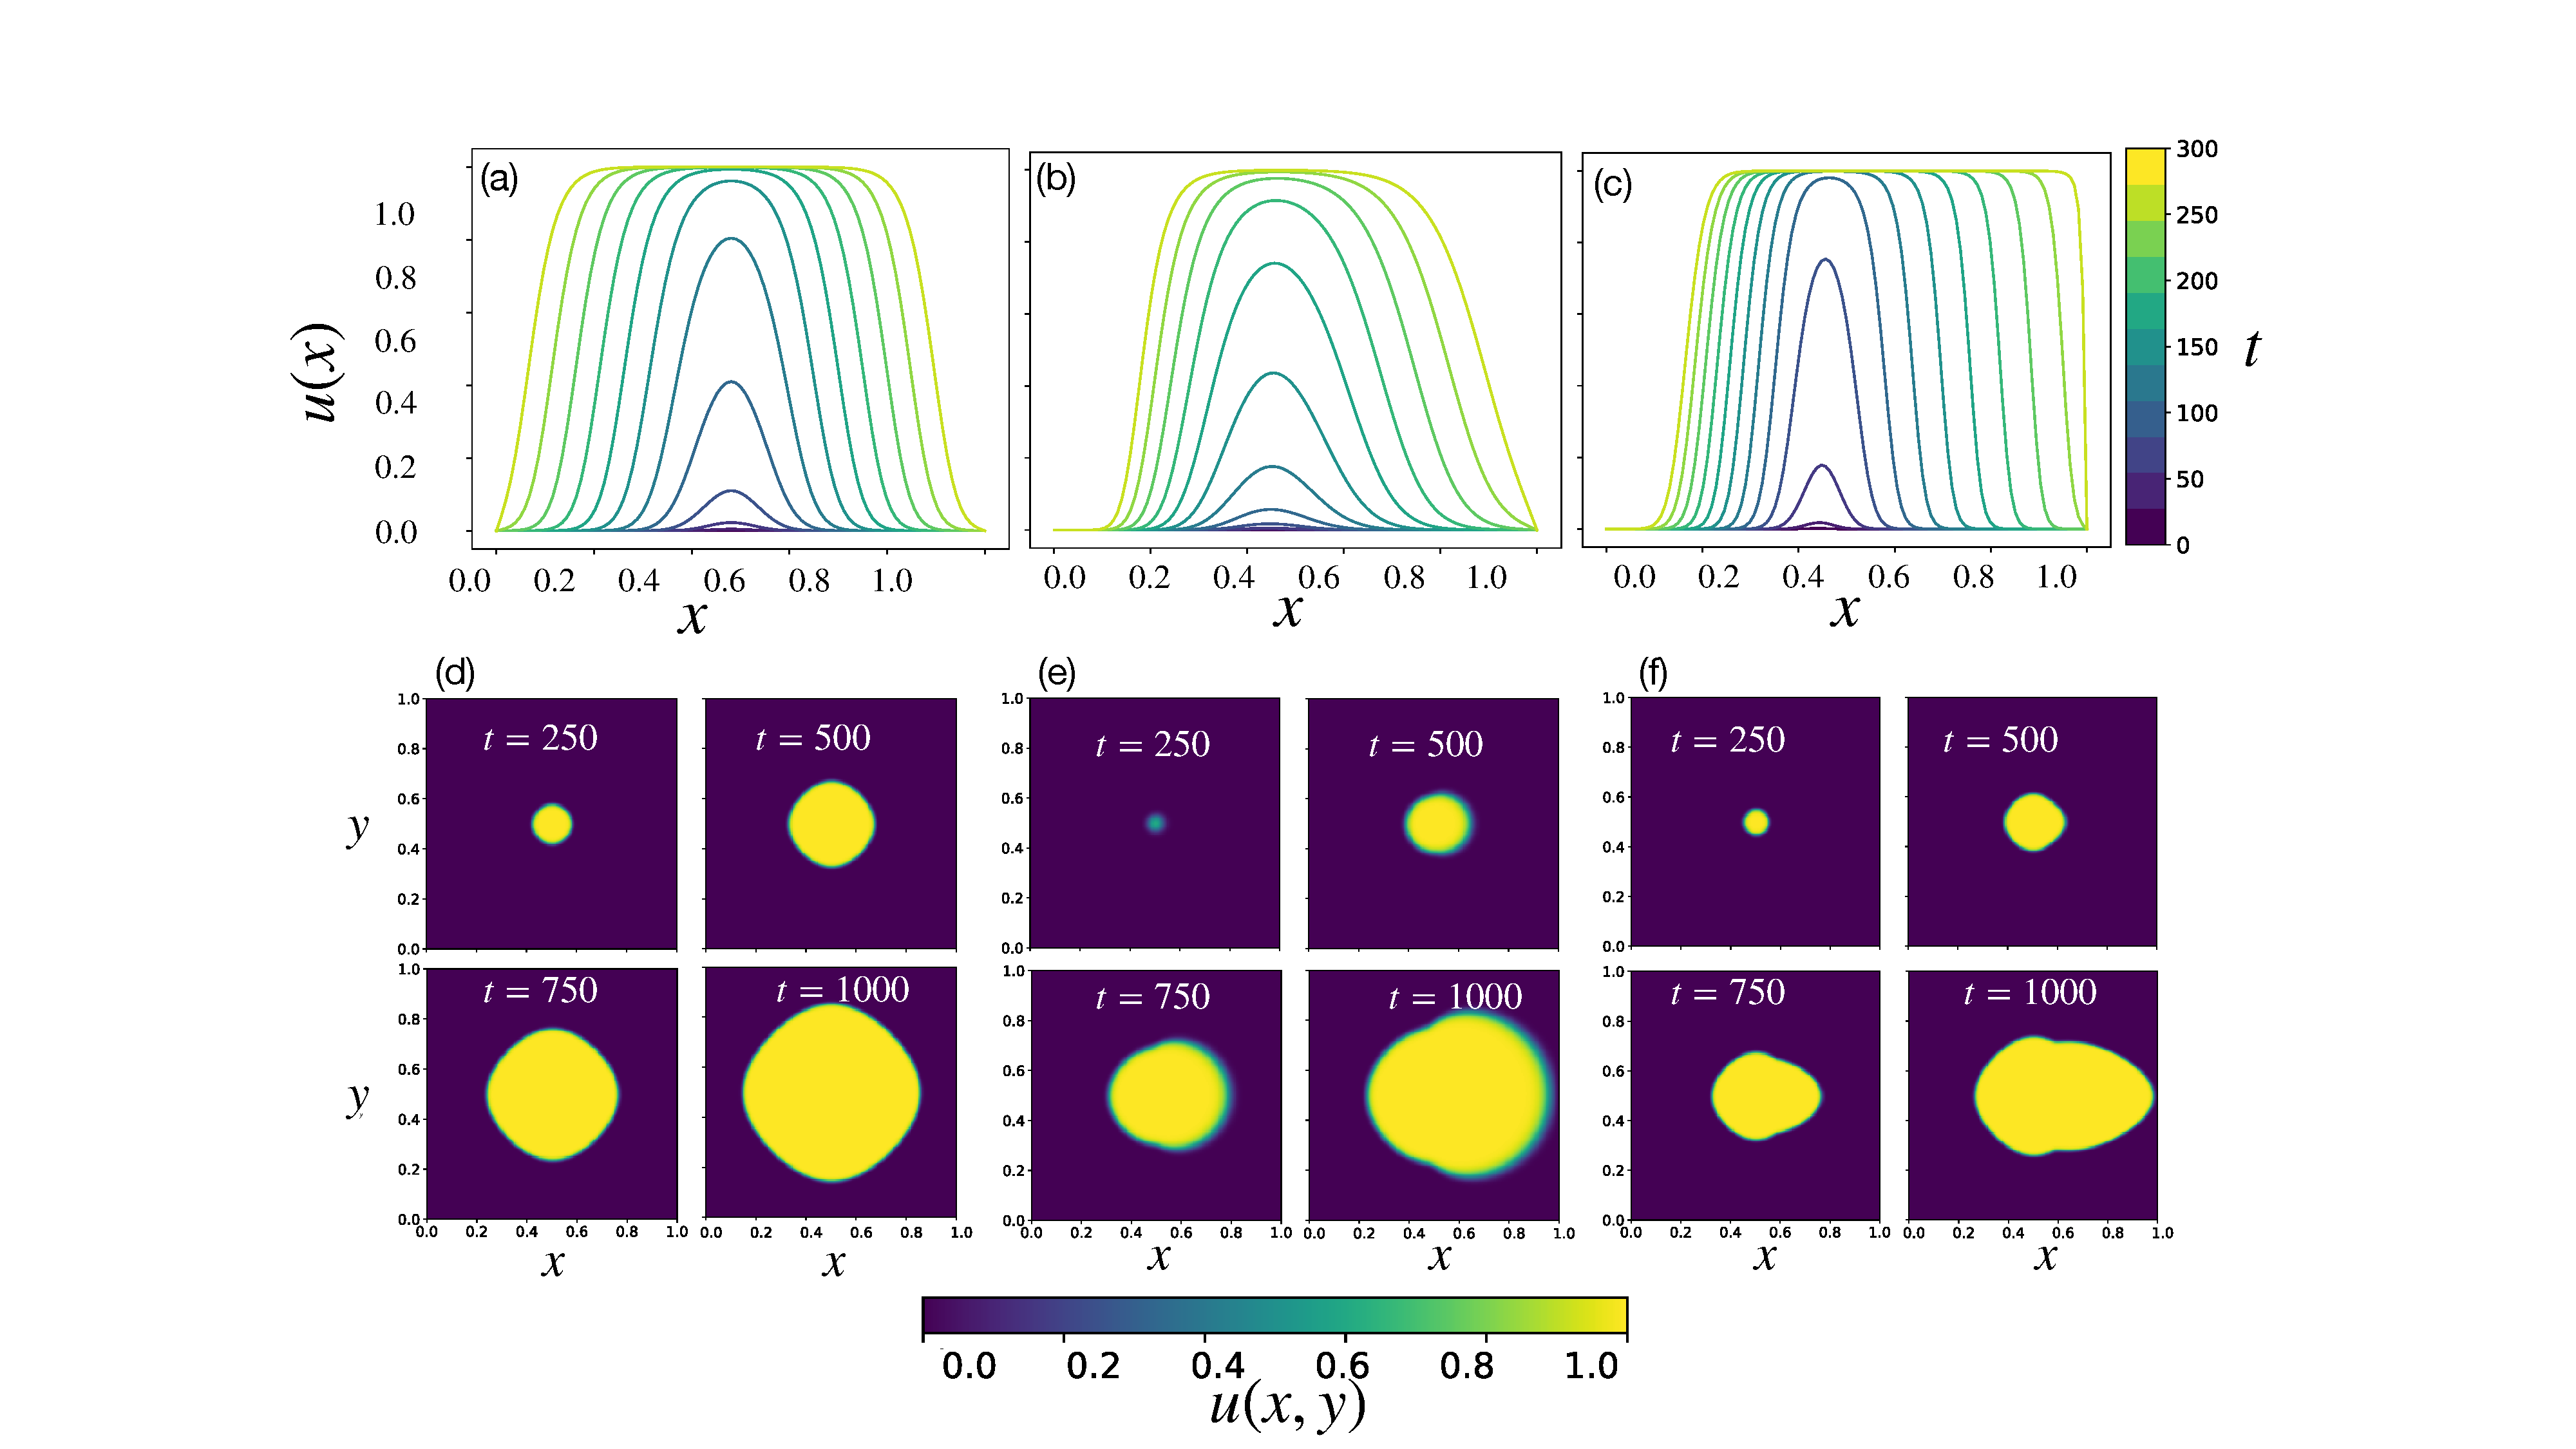
\includegraphics[scale=0.325]{chapter2/figures/FKPP.pdf}
    \caption{
    A simulations of the FKPP model for $r=0.10$ and $\mathcal{D}=0.10$ in one spatial dimension. 
    A non-zero field value is initialised at $x=10$ at time $t=0$. Uniform growth and diffusion 
    give rise to a wave-front that propagates with constant speed.}
    \label{fig:fkpp-expo1D}
\end{figure}

\blindtext


% initially travelling waves... 
% describe FKPP...
% power law dispersal... \cite{severns2019consequences} accelerating fronts...


% \textcolor{red}{
% \begin{itemize}
%     \item review \cite{doi:10.1098/rsif.2005.0051}
% \end{itemize}}

% \subsection{Diffusion}

% \cite{mundt2009long}  \cite{mundt2009aerial}

% In one spatial dimension, the FKPP model is given by:
% \begin{equation}
%     \frac{\partial u}{\partial t} = \mathcal{D}\nabla u + ru(1 - u/K)
% \end{equation}
% where $\mathcal{D}$ is a diffusion coefficient measured in units $\mathrm{m^2 t^{-1}}$ 
% and $r$ is a growth constant (or rate) with units $t^{-1}$. 
% This model assumes logistic growth and diffusion, where the field $u$ represents a `concentration',
% and $K$ represents the carrying capacity, when $u=K$, the system growth goes to zero.

%\item \cite{doi:10.1098/rstb.1998.0226} gave a three population (host, parasite and hyperparasite), which considered transmission via a reaction-diffusion process.

% \textcolor{red}{
% \begin{itemize}
%     \item Spatial SIR model
%     \item Agent-based modelling
%     \item A good place to talk about Percolation models
%     \item \textcolor{red}{Murray}: travelling waves that do not change shape
% \end{itemize}}

\section{Tree distribution datasets in Great Britain}
\label{ch2:hostdata}

Large-scale epidemic models of tree disease rest on robust, high-quality host data.
Data-driven approaches are crucial for predicting disease spread over country-wide scales, 
though collecting high-quality host data involves myriad challenges. 
Most notably, large-scale species distributions require vast datasets that demand significant economic resources
and person-hours to assemble and maintain over time. 
However, satellite-based remote sensing technologies pose an attractive solution\textemdash see \cite{camarretta2020monitoring} for a recent review of remote sensing technologies.
Despite the significant advances of remote sensing technologies, most freely available data sets still rely on traditional surveying methods to collect data throughout Great Britain (GB).
Consequently, the most widely known and widely used datasets are reviewed below.
Following this, statistically-generated species distribution models, typically based on surveyed data, are reviewed.

\subsection{National Surveys}

Surveyed data predominantly describes either: abundance, presence-only, presence-absence data. 
Generally, abundance data describes percentage canopy cover per $\mathrm{km^2}$.
In contrast, presence-only and presence-absence data that record if a species is present or present and absent, respectively.
Abundance captures significantly more information than presence-only data, yet unfortunately, they are in short supply.

\subsubsection{Countryside Survey}

The countryside survey (CS) is a long-running, national survey of diversity and species abundance in GB \cite{wood2017long}.
The UK Centre of Ecology and Hydrology (UKCEH) undertakes the surveys, primarily funded by the Natural Environmental Research Council alongside other government agencies.
Individual surveys have been undertaken in: $1978$, $1990$, $1998$, $2007$, and $2019$. 
Random stratified sampling captures a representative species abundance\footnote{
A useful (unpublished) project merged abundance data from CS with myForest. The abundance data can be found at the Oxford University research archive: \nolinkurl{https://ora.ox.ac.uk}.} 
over of all land cover compositions, e.g. lowland acid grassland, freshwater, and broad-leaf forest.

Abundance data is collected for numerous dominant species, including trees, shrubs, ground flora and soil type, 
making the scope of CS data vast. Moreover, long-running records spanning decades reveal ecosystem trends imperative for ecological monitoring.
More recently, $100$ $1\mathrm{km^2}$ plots of vegetation and soil data were collected\footnote{
The data is free to download on the UKCEH website: \nolinkurl{https://catalogue.ceh.ac.uk}} \cite{10.5285/fd6ae272-aeb5-4573-8e8a-7ccfae64f506}.
The dataset constitutes the first of five planned surveys, part of a rolling monitoring strategy collected every five years.

\subsubsection{National Forest Inventory}

\begin{figure}
    \centering
    \includegraphics[scale=0.2]{chapter2/figures/NFI-figure.pdf}
    \caption{NFI data super imposed onto a Google earth image, taken from a report (unpublished) by S. Orozco-Fuentes et al.
             NFI data covering Thetford Forest Park ($16.684 \mathrm{km}^2$) is shown as a polygon in the NFI `woodland' category.
             Data is interpreted as the conifer forest type. Here, surveys comprises presence-only data, and no tree species percentage cover
             is reported. NFI data extends throughout $\sim 13\%$ of land coverage in GB and large non-woodland areas remain un-surveyed.}
    \label{fig:NFI-data}
\end{figure}

The National Forest Inventory (NFI) collects and maintains forest and woodlands data in GB.
Originally, the NFI was established to help restore and expand Britain's woodlands following the First World War \cite{james1990history}.
Regular programs ($10$-$15\mathrm{year}$ intervals) implement surveys of woodland and forest size, distribution, composition and condition across GB.
Records cover areas over $0.5\mathrm{ha}$ and $20\%$ coverage.
As of $2019$, $622,381$ individual records exist, spanning $2.9 \times 10^6 \mathrm{ha}$ over $13\%$ of the total land cover within GB.
NFI data comprise ESRI shape files\footnote{
Free to download at: \nolinkurl{https://data-forestry.opendata.arcgis.com}},
that outline numerous forest types, e.g. broadleaved, conifer, mixed-predominantly broadleaved or mixed predominantly conifer.
Despite an extensive coverage, publicly available NFI surveys describes presence-only data\textemdash with no proportion or species coverage.
Although, additional datasets are available to purchase, including: 
1) Tree species percentage per region by woodland type
2) Tree species proportions within the upper canopy of each NFI sample plot, without supplying the exact location of the individual sample plot.

\subsubsection{Botanical Society of Britain and Ireland}

\begin{figure}
    \centering
    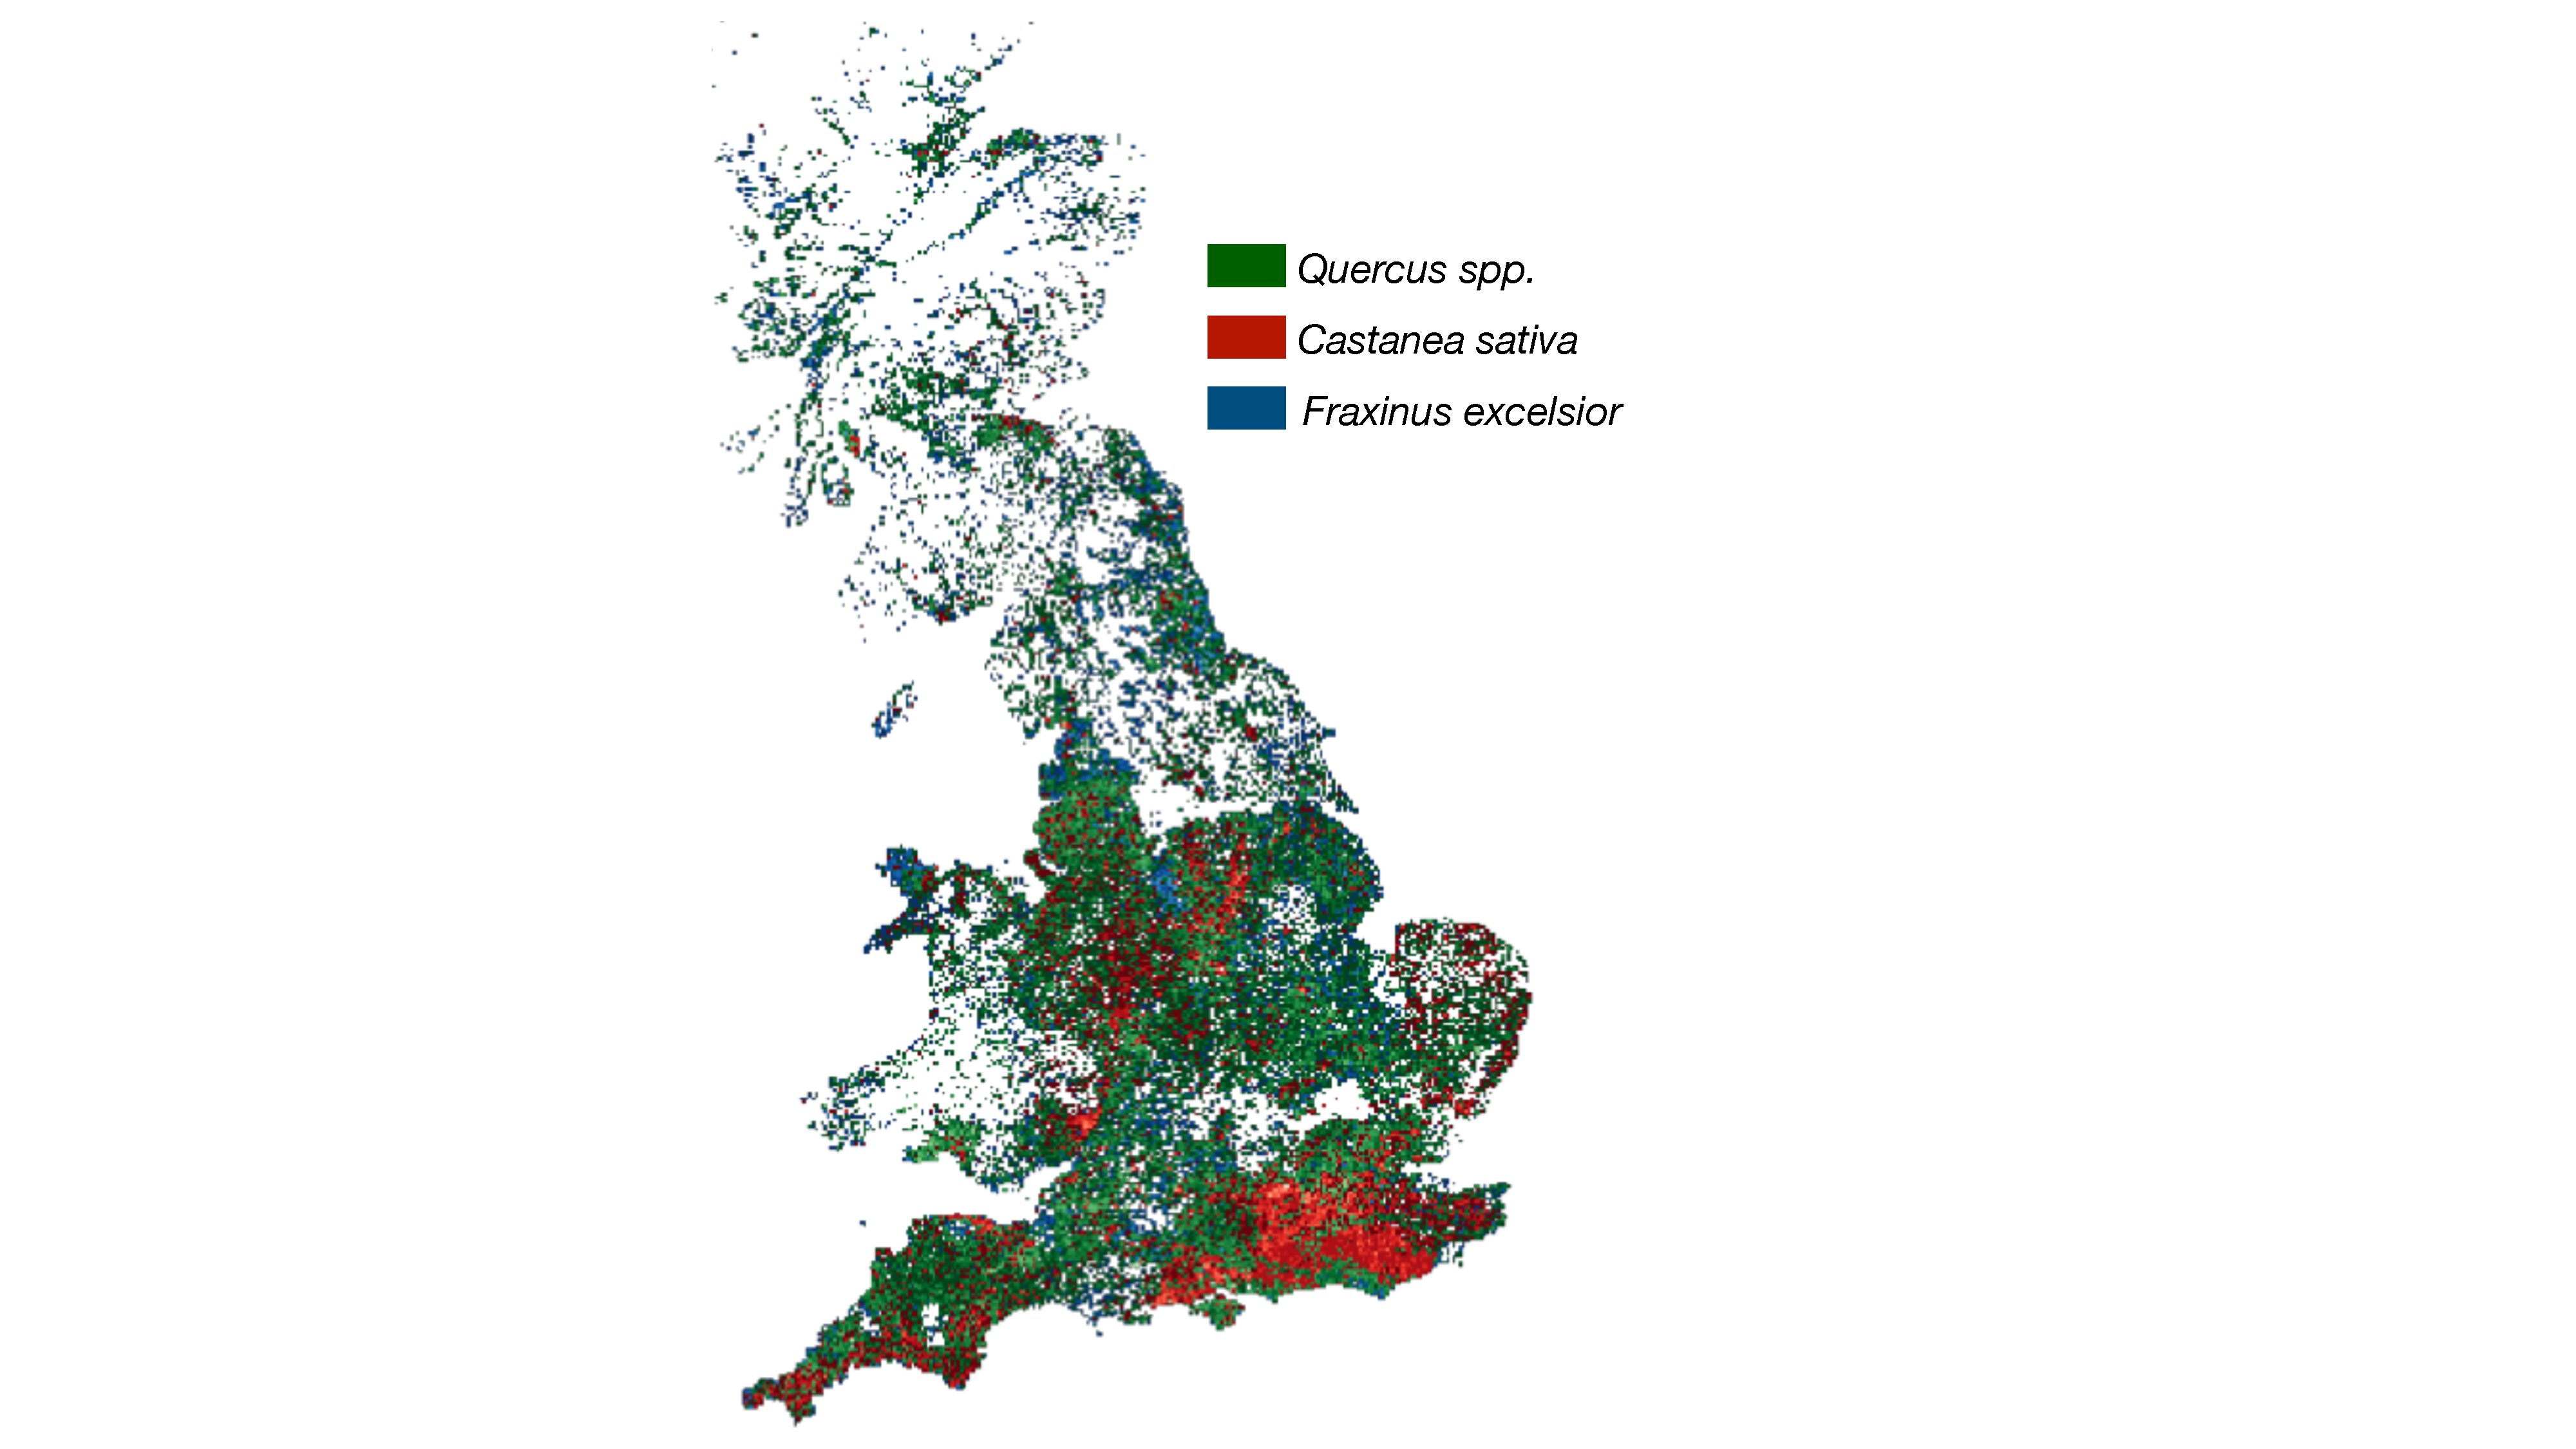
\includegraphics[scale=0.25]{chapter2/figures/bsbi-data.pdf}
    \caption{BSBI presence-only datasets\textemdash as reconstructed by S. Orozco-Fuentes et al. (unpublished).
    Three important large deciduous tree species, European ash (\textit{Fraxinus excelsior}), 
    Oak (\textit{Quercus spp.}), and sweet chestnut (Castanea sativa), are overlaid onto the same map at $\mathrm{2km \times 2km}$ resolution.
    The BSBI datasets are extensive and report presence-only data over a country-wide scale.
    }
    \label{fig:bsbi-data}
\end{figure}

The Botanical Society of Britain and Ireland (BSBI) has recorded species presence-only data since $1950$.
BSBI datasets are publicly available\footnote{BSBI data can be downloaded from: \nolinkurl{https://database.bsbi.org}.} upto a
resolution of $\mathrm{2 km \times 2km}$, though records upto $\mathrm{100 m \times 100 m}$ are available to registered members.
As of $2020$, BSBI records are collected at $\mathrm{1 km \times 1km}$ square resolution or better\textemdash making the datasets among the 
highest-resolution surveys collected by traditional methods. The BSBI distribution database contains records of plants and charophytes
as reported by users and conservationists with MapMate\footnote{MapMate is software designed to aid users to share ecological data: \nolinkurl{https://www.mapmate.co.uk}}.
Despite the availability of high-resolution data, observations are collected ad hoc by users and not curated scientifically.
Moreover, the distributions contain both well-surveyed and poorly-surveyed plots of land likely to carry uncertainties.
As such, BSIBI data is helpful to reconstruct several baseline tree distributions across GB, as demonstrated by \cite{hill.data}.

\subsection{Species distribution models}

\begin{figure}
    \centering
    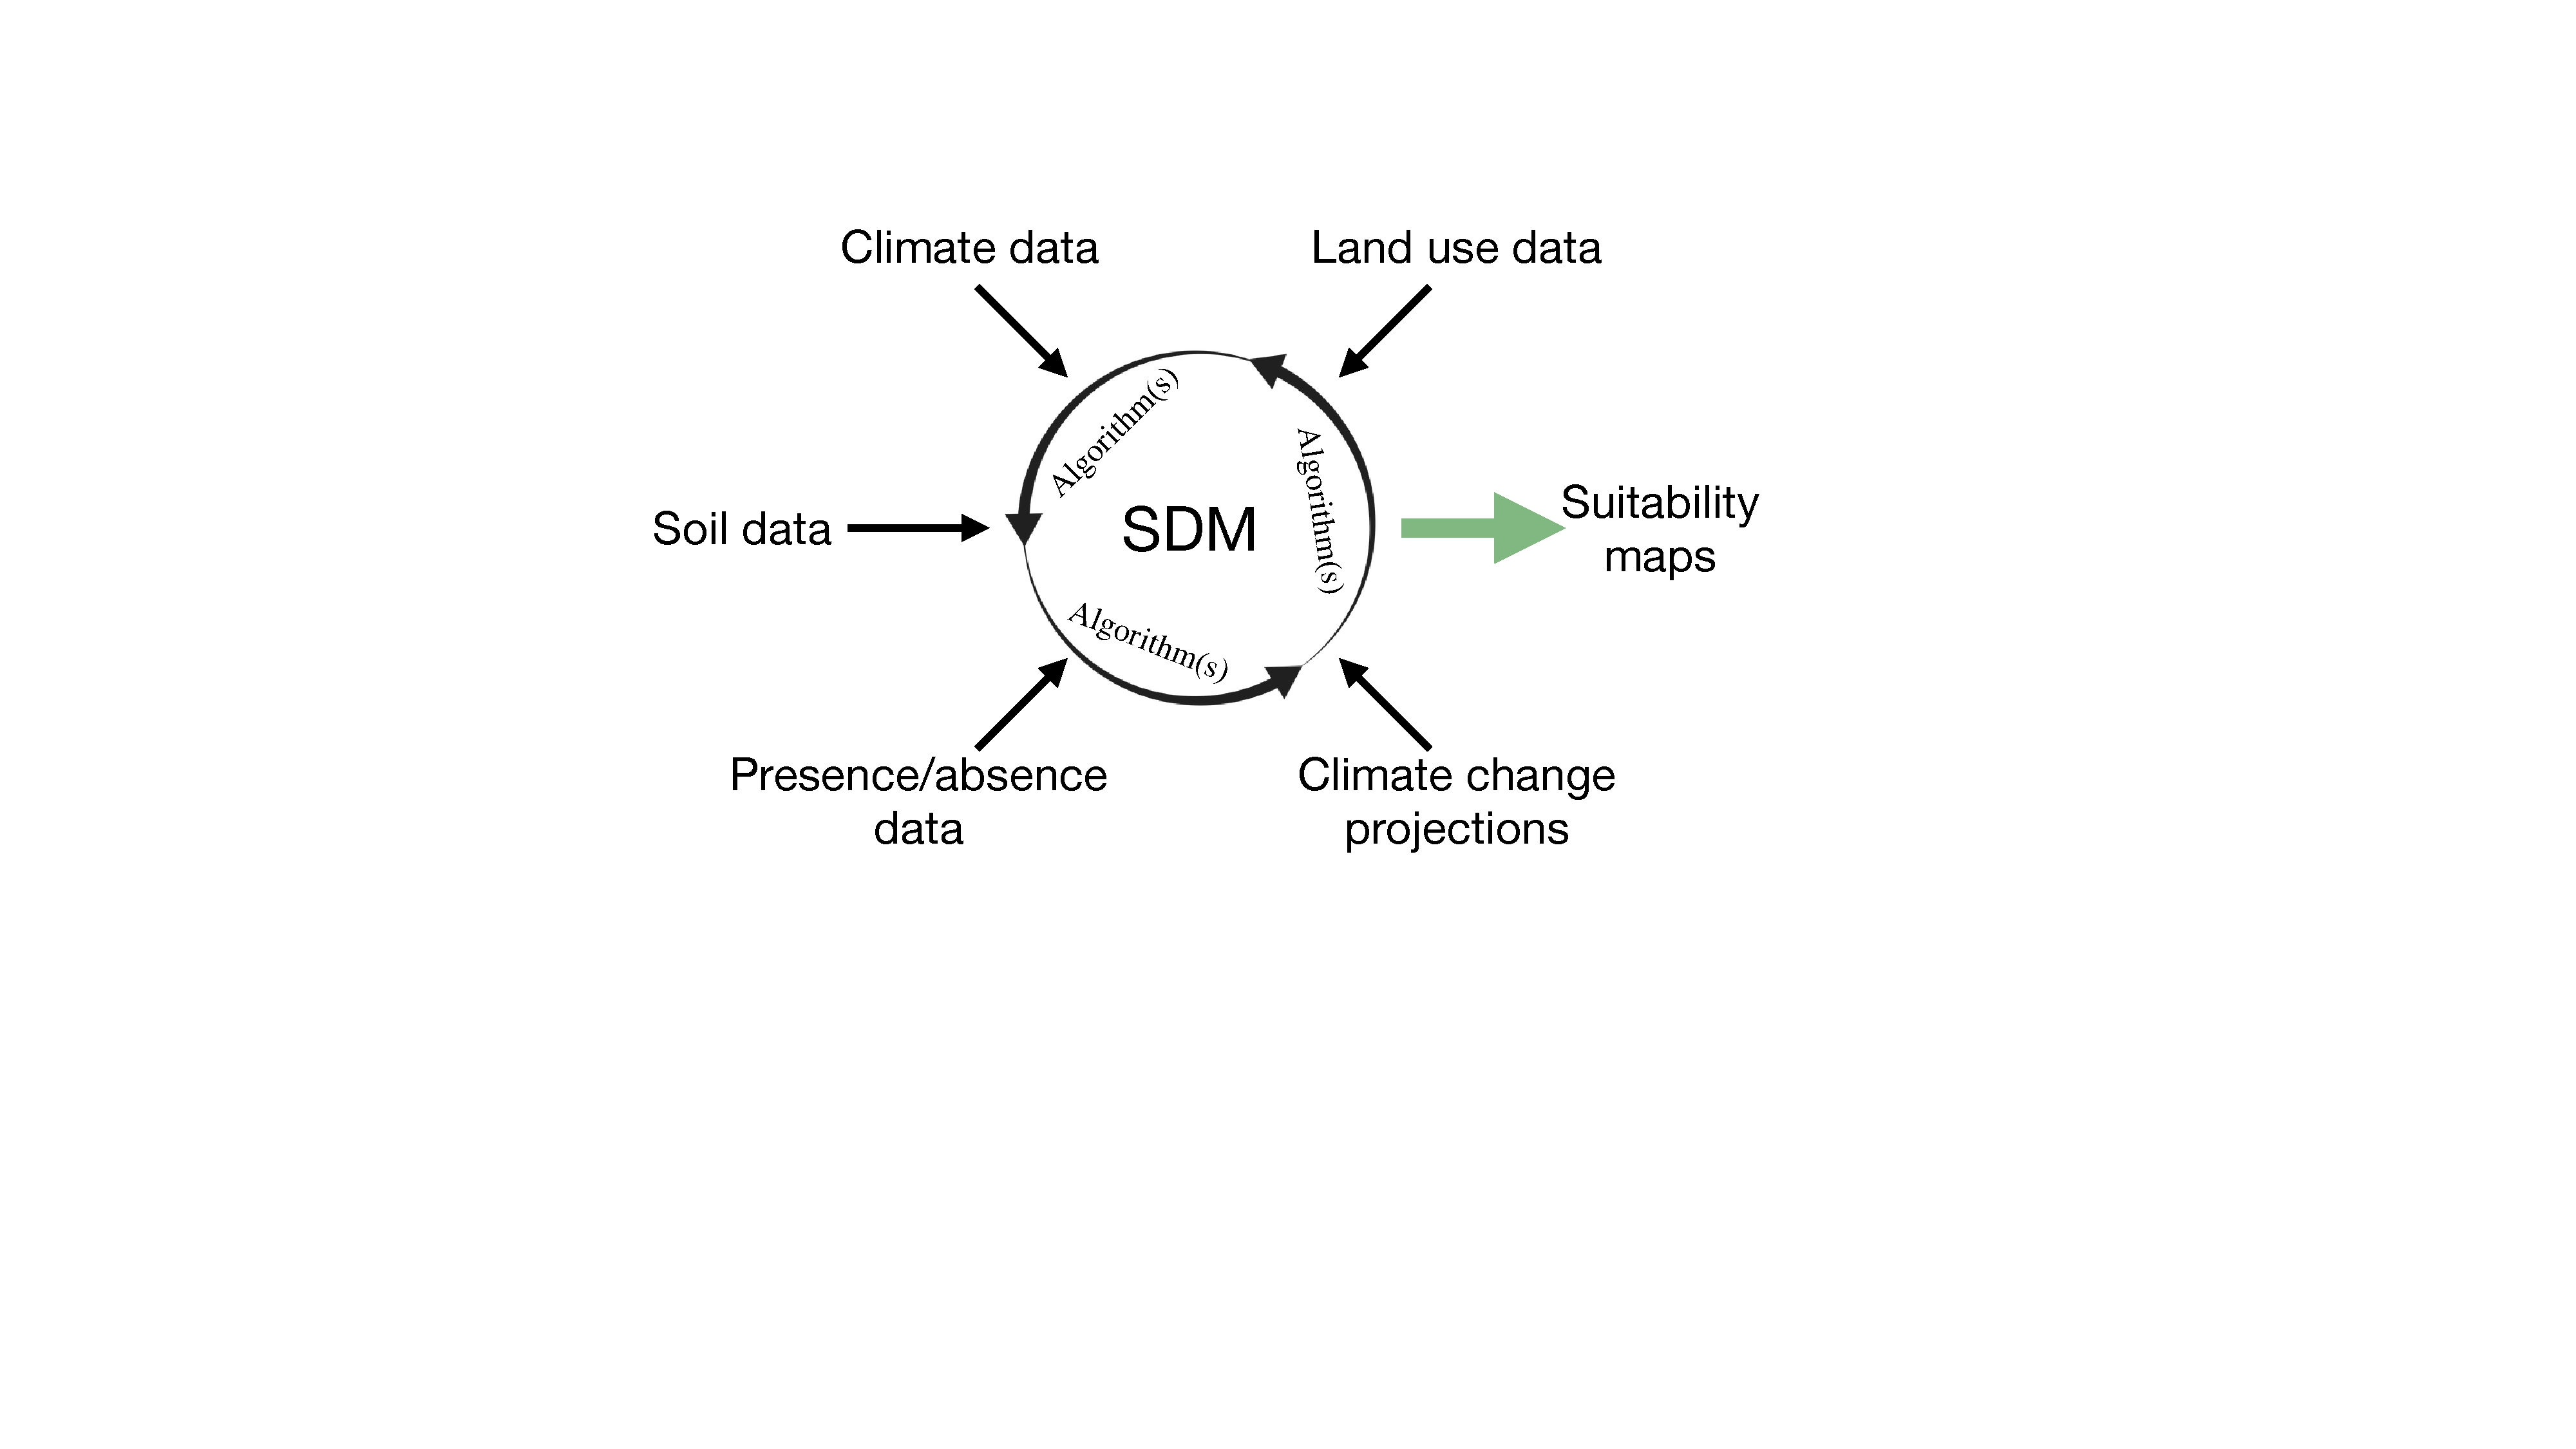
\includegraphics[scale=0.35]{chapter2/figures/SDM-fig.pdf}
    \caption{A graphical species distribution model (SDM) illustration, adapted from \cite{SDM_1}. 
             A variety of predictor variables and input data sources are used in conjugation with modelling algorithms to produce
             a habitat suitability map.}
    \label{fig:sdm}
\end{figure}

Species distribution models (SDMs) aim to generate data, from less-extensive surveyed data.
SDMs were first developed in the $1990$s, and have subsequently become fundamental to ecological and biogeographical inference studies.
Inferred, or modelled, species distribution data have been used to examine biodiversity, conservation, resource management, 
ecology and climate change \cite{austin2011improving, franklin2013species, skov2016real, wittmann2016confronting, 10.3958/059.037.0110, zhang2019using}.
The vast majority of SDMs fall into two categories: correlative \cite{srivastava2019species}, and mechanistic \cite{shabani2016comparison}.

Correlative SDMs relate (widely available) presence-only, or presence-absence, data to several environmental predictor variable datasets.
For tree species, predictor variables include temperature, precipitation, altitude, and soil type \cite{ray2021multi, hill.data}.
Following this, a species distribution map can be predicted, albeit with  uncertainties and errors.
Commonly used statistical methods include Regression 
(i.e. General Linear Models, General Additive Models, Multivariate Adaptive Regression Splines) and Machine Learning
(i.e. Artificial Neural Networks, Classification And Regression Tree, Random Forest). 
The general correlative approach is reflected in Figure \ref{fig:sdm}; for a more in-depth review of correlative SDMs, see \cite{SDM_1}.

Correlative SDM approaches require little to no prior knowledge of the physiological processes that link organism and environment.
Hence, mechanistic methods aim to incorporate an organisms behavioural, physiological, and morphological constraints to the environment, 
as reviewed by \cite{kearney2009mechanistic}. However, linking a species physiological response to the environment comes with significant
computational challenges, as it typically relies on vast, multi-variable time-series datasets \cite{shabani2016comparison}.

A review paper by \cite{guillera2015my}, revealed a diverse use of SDMs.
Out of $100$ publications reviewed by \cite{guillera2015my}, SDMs were applied to: 
1) managing threatened species ($16\% $ of articles) 
2) predicting climate change impacts ($13\%$) 
3) understanding phylogeographic patterns ($9\%$) 
4) controlling threatening processes ($8\%$) 
5) landscape management ($8\%$) 
6) biological invasions ($7\%$). However, no epidemic applications were reported.

Nevertheless, a thorough literature search revealed a variety of epidemiological SDM applications.
The crossover between ecological SDM methods and epidemiology has been referred to as `Infectious Disease Cartography' \cite{KRAEMER201619}.
With Infectious Disease Cartography, one seeks to map the likelihood, or risk, of infectious disease outbreaks and produce risk-maps.
A number of publications have applied SDMs livestock diseases \cite{hollings2017species}, and human-based diseases including the global 
distribution of Dengue Fervour \cite{bhatt2013global} and Zika virus \cite{messina2016mapping}, and Anthrax in Kenya \cite{otieno2021modeling}.
However, SDM applications for tree disease epidemics appear absent from the literature.

\subsubsection{Modelling tree abundance}

SDM-generated tree occurrence data has limited applications to ecologists and forest managers.
This motivates a statistically-generated abundance data, that includes significantly 
more information about the population occupation/density and ecosystem.
Modellers have examined numerous approaches to predict species abundance;
including, linking the abundance-occupancy relationship \cite{gaston2000abundance} and
the scaling pattern of species occupancy over progressively smaller spatial scales \cite{hui2009extrapolating}.

An interesting, and highly relevant, approach to predict the abundance of common tree species in Great Britain was put forward by \cite{hill.data}.
At a high level, (BSBI) presence-only data was combined with a series of environmental covariates using a species distribution model to 
produce a map of predicted occurrence data. Then, random forest regression was employed with a training sample ($70\%$) of less extensive abundance 
data\textemdash consisting of Countryside survey, myForest and Bluesky's National Canopy Map. 
Results were then cross-validated with the remaining ($30\%$) abundance data; Figure \ref{fig:hill-method} displays a
flow-diagram of the method presented by \cite{hill.data}. 

A more detailed explanation of the treatment proposed by \cite{hill.data} follows:
\textbf{Stage 1)}
\textit{
\begin{itemize}
    \item Presence-only BSBI data was downloaded for $25$ common species of trees in GB, 
    and all records less than $\mathrm{2km \times 2km}$ resolution were discarded.
    Next, the presence-only data was converted into presence-absence data by considering
    `well-surveyed' records that Hill et.al defined as having a minimum of two survey
    between $1950$ and consisting of $50$ species. Species missing from these 
    well-surveyed areas were assumed truly absent. 
    \item Using biomod2 \cite{thuiller2016package}, a SDM was then fitted against a cohort of 15 environmental variables, e.g.
    soil type (European Soil Database), temperature (Worldclim), precipitation (Worldclim), altitude (Worldclim),
    type of land cover (Countryside Survey), among others. The net result was a map of predicted occupancy at $\mathrm{1 km \times 1 km}$ 
    resolution.
    \item For each species, predictions from a suit of models\textemdash GLM, GAM, CTA, GBM, RF\textemdash were
    repeated and combined into an ensemble distribution model. Each model was cross-validated against
    $30\%$ of the well-survyed BSBI presence-absence data using the receiver operator curve (ROC) and the true skill statistic (TSS).
    \cite{hill.data} then selected the best performing predicted occurrence for each species.
\end{itemize}
}
\textbf{Stage 2)}
\textit{
\begin{itemize}
    \item Abundance data from Countryside survey (CS) and myForest were both expressed as hectares covered per kilometer 
    squared ($\mathrm{ha/km^2}$). This entailed using woodland cover data from the National Forest Inventory (NFI) to multiply
    the percentage cover of each species within a woodland patch, with a proportion of woodland cover per kilometer.
    \item Random forest (RF) regression then modelled the relationships between (CS and myForest) abundance data with
    the SDM-generated map of predicted occupancy. In addition, RF regression used four covariates, 
    three of which consisted of Bluesky's National Canopy data (i.e. total tree cover, woodland tree cover, non-woodland tree cover)
    and NFI edge broadleaved woodland (i.e. within $50\mathrm{m}$ of non woodland) data.
\end{itemize}
}

The abundance datasets produced by \cite{hill.data} combine several mainstream tree datasets in GB; moreover, 
constructing the ensemble model involved a variety of statistical models.
The predicted occurrence data was examined against the Receiver operating characteristic (ROC) \cite{jimenez2012insights}.
Most species demonstrated functional ROC scores between $0.71$ and $0.96$ and performed exceptionally
well for ash ($0.96$) and oak ($0.90$).  

Although, numerous assumptions underpinned the method of predicting occupancy.
Primarily, the BSBI dataset used by \cite{hill.data} exists through ad-hoc user and volunteer self-reports.
Thus, some regions are more surveyed than others over the years, this led Hill et al. to make the 
`well surveyed' recorded assumption (i.e. only considering records surveyed twice since $1950$ containing a minimum of $50$ species).
The assumption permitted the conversion of raw presence-only to presence-absence, 
at the cost of overestimated absence in these regions. That is, even supposing $50$ species
are reported within a subset of the ($\mathrm{2km \times 2km}$ tetrad) record, other large regions could remain unsampled. 
We remark the authors did not appear to scrutinise this assumption sufficiently.

\begin{figure}
    \centering
    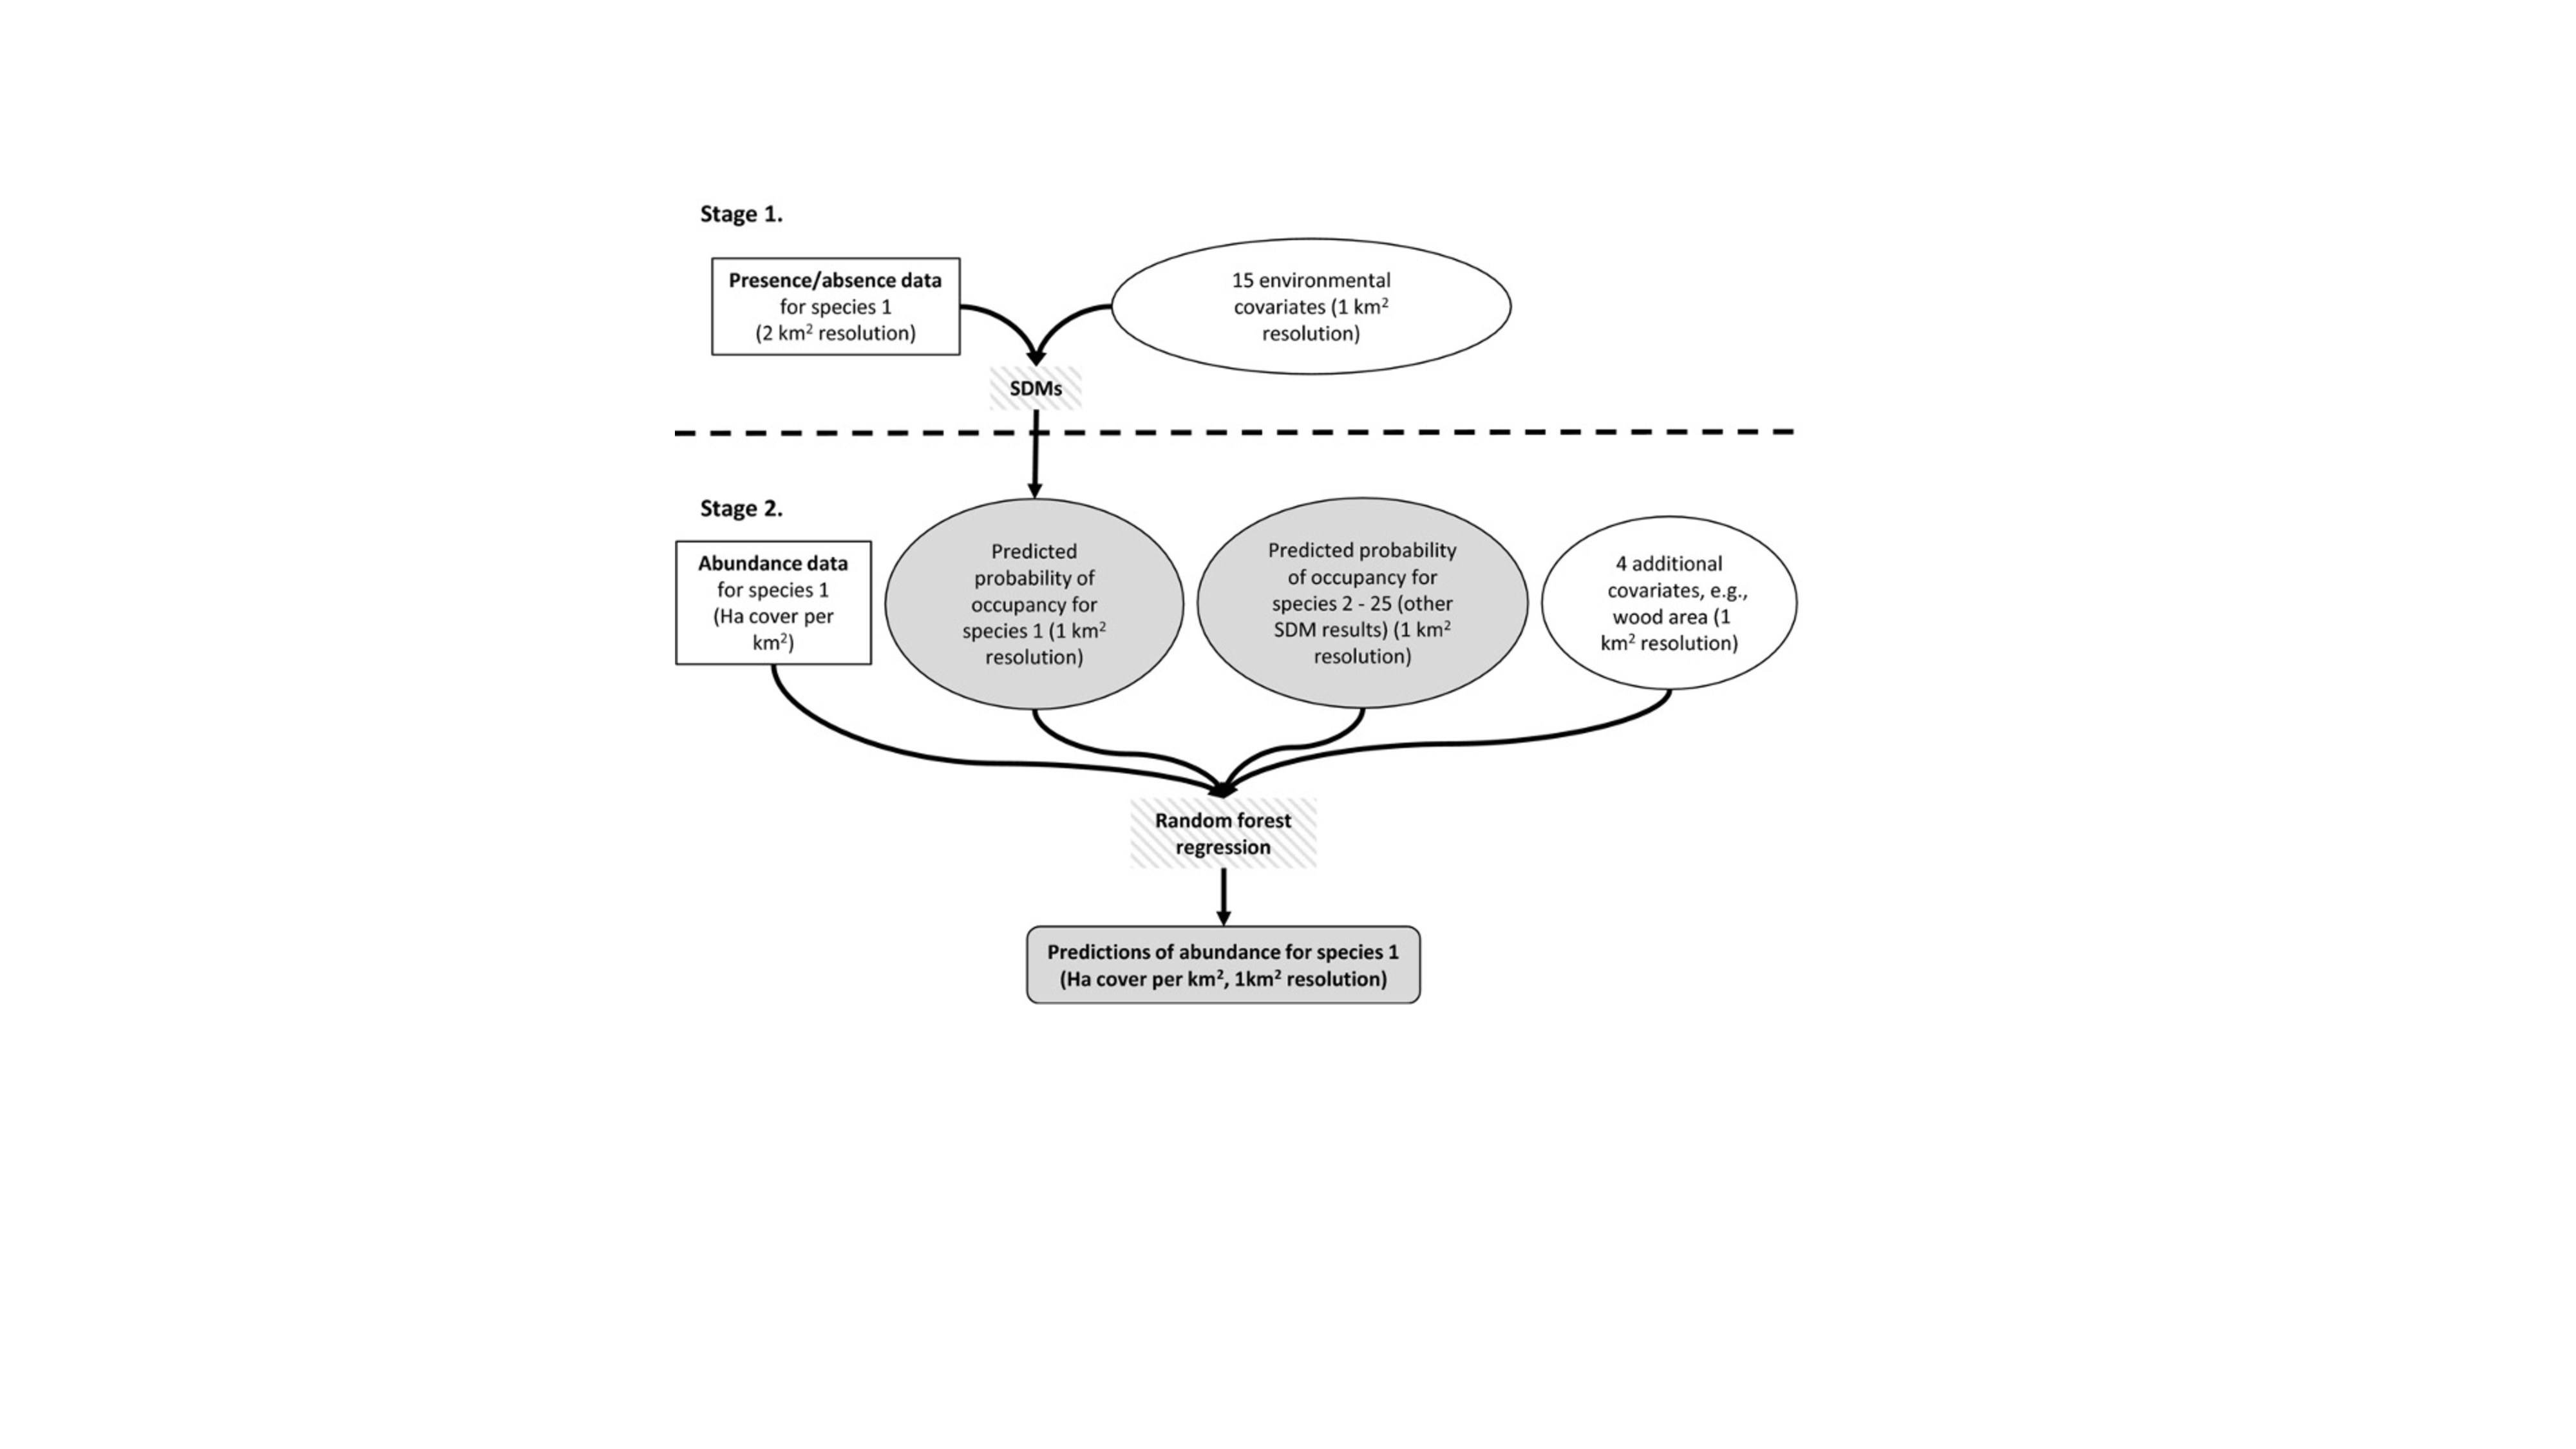
\includegraphics[scale=0.55]{chapter2/figures/hill-method-fig.pdf}
    \caption{A flow diagram of the two-stage abundance method put forward by \cite{hill.data} to model tree species abundance  
    (taken from the publications' materials and methods section).}
    \label{fig:hill-method}
\end{figure}

The RF regression used by \cite{hill.data} marked a novel approach to modelling species abundance.
The authors chose to argue in favour of RF regression because of its insensitivity toward the data distribution,
which worked well with the less comprehensive abundance data sources (as the map of abundance had a high percentage of zeros from missing records).
The abundance model quality was examined against $10$-fold validation (explained in \cite{refaeilzadeh2009cross}).
The root-mean-square error (RMSE), between predicted and observed abundance, generally ranged between $5$ and $10$,
where the RMSE scale reflects the response variable units ($\mathrm{ha/km^2}$), i.e. $5\%$ and $10\%$ respectively.
The result was country-wide predicted abundance.

The low amount of available abundance data in GB significantly impoverished the abundance maps produced by \cite{hill.data}. 
Consequently, datasets for the $25$ species considered will contain numerous (small-scale) errors and uncertainties. 
Nonetheless, the modelled abundance maps captured more large-scale spatial structures than the original BSBI and CS distributions.
More recently, \cite{ray2021multi} produced a similar SDM as Hill et al. for oak in GB using biomod2 \cite{thuiller2016package}.
The authors focused on mapping high-density oak woodlands (with 60$\%$ canopy cover or above) 
to predict which NFI map polygons (by forest type) were most likely to contain oak stands. 
However, \cite{ray2021multi} did not make their oak maps publicly available, nor did they produce a general-purpose
abundance map relevant for epidemiological studies. 
To date, the predicted abundance maps produced by \cite{hill.data} constitute the best publicly available 
country-wide maps in GB, despite their limitations.

%\item remote sensing tools were used \cite{kelly2002monitoring} to track the study of sudden oak death in California
%\item \cite{kelly2002landscape} demonstrated clustering at the landscape level, spatial structure is important

\section{Ash dieback case study}

% - the combination of ash dieback and emerald ash borer present a significant threat to UK and European ash \cite{musolin2017between}
% - managing the spread of ADB in areas already infected is hardly possible \cite{gross2014h}
% - but slowing the spread of disease is still valuable to allow ash populations vital time to recover and policy makers \cite{PAUTASSO201337}
% - multi-scale approaches have been outlined \cite{hart2020theoretical}

\label{ch2:ash-dieback}
Ash dieback (ADB) presents an interesting case study of an emerging epidemic currently devastating ash
populations throughout Europe \cite{enderle2019overview}. The history and predicted evolution of ash dieback
demonstrate how an invasive, non-indigenous pathogen can spread rapidly through a foreign ecosystem that 
lacks evolutionary defences. Among the many factors driving the spread of ash dieback, long-distance 
anthropomorphic trade is the mechanism responsible for the initial introduction into Europe from the
far-east \cite{zhao2013hymenoscyphus, queloz2011cryptic}.

The pathosystem has been the subject of much research over the years. As a result, the taxonomy, 
symptoms and life-cycle of the pathogen are  now well-known \cite{https://doi.org/10.1111/mpp.12073}. 
Understanding the spread of ADB and managing the epidemic impact on ecosystems could only be achieved
by the confluence of molecular biologists, forest managers, policymakers and modellers. Although the epidemic
is well underway, slowing the spread of ash dieback remains essential to allow ash populations time to adapt.

\subsection{Historical developments}

Reports of dieback on ash began surfacing in Poland in $1992$, but a causal agent was not established
for a decade \cite{kowalski2001zamieraniu, coetsee2000xenochalara}. Subsequently, \cite{kowalski2006chalara} 
recognised a novel pathogenic fungus to be the causal agent, identified as an ascomycete anamorph (i.e. an asexual fungus).
The fungus was named \textit{Chalara fraxinea}, a member of the hyphomycete genus \textit{Chalara}. 
The sexual teleomorphic stage of the pathogen was later attributed to \textit{Hymenoscyphus albidus} 
\cite{kowalski2009teleomorph}, a well-known non-pathogenic fungus indigenous to Europe.

Linking the hitherto non-pathogenic \textit{H. albidus} to the agent causing ash dieback perplexed researchers. 
The enigma was resolved through DNA sequencing by \cite{queloz2011cryptic} when a second morphologically identical
ascomycete named \textit{`Hymenoscyphus pseudoalbidus'} was identified as the pathogen responsible for widespread dieback
of European ash in a process referred to as `Cryptic speciation'.

Interestingly, the emergent epidemic caused by \textit{H. pseudoalbidus} coincided with developments 
in the phylogenetic classification system of the kingdom Fungi \cite{hibbett2007higher}, 
and dual nomenclature\footnote{Originally, fungi were classified through the structure of their sexual organs.
Problematically, ascomycete fungi have a complicated dual reproductive mode (both sexual and asexual) that often caused confused. 
However, a move toward a one-name fungi classification system has since simplified fungi taxonomy.} 
\cite{wingfield2012one}. Subsequently, the pathogen \textit{`Hymenoscyphus pseudoalbidus'} was renamed to
\textit{Hymenoscyphus fraxineus} (HF).

\subsection{Symptoms and epidemiology}

European ash is highly susceptible to HF because it has no (co-evolved) evolutionary defence.
Although HF is lethal to European ash, it poses little threat to its native Asian hosts 
\textit{Fraxinus mandshurica} and \textit{Fraxinus chinensis}. Once the fungus colonises a European ash leaf,
it can spread through twigs, branches, the xylem, and eventually the whole tree.
The symptoms include necrotic lesions, crown dieback, wilting and eventual death.
In addition to leaf-infections, the pathogen can colonise the root-system \cite{schumacher2011general}.
Root-infections usually occur in already severely infected ash \cite{https://doi.org/10.1111/mpp.12073}. 
After which, it is only a matter of time before opportunistic fungi invade and significantly accelerate mortality
\cite{enderle2013temporal}.

The progressive symptoms of ADB, as presented by \cite{gross2014h}, are displayed in Figure \ref{fig:ash-deiback-symptoms}.
Ascospores initially infect susceptible ash leaves (a), 
becoming visible after around two weeks \cite{https://doi.org/10.1111/ppa.12048} in the summertime. 
In Figure \ref{fig:ash-deiback-symptoms}, panels (b-d) show the initial infection spreading through 
the leaf into the rachis and the development of the first necrotic lesions\textemdash see
\cite{https://doi.org/10.1111/ppa.12844} for further information on the precise mechanism of ascospore leaf penetration.

Over winter, the infection continues to spread through ash. 
Young ash develop large visible necrotic lesions, as illustrated in Figure \ref{fig:ash-deiback-symptoms}(e-i).
In spring, the infection causes shoot wilting (g) and death (h-i) before causing xylem necrosis (j).
Over many seasons, large infected mature ash trees begin to die (l) as it begins forming epicormic branches, 
as noted by \cite{marciulyniene2017can} and losing its canopy.

\begin{figure}
    \centering
    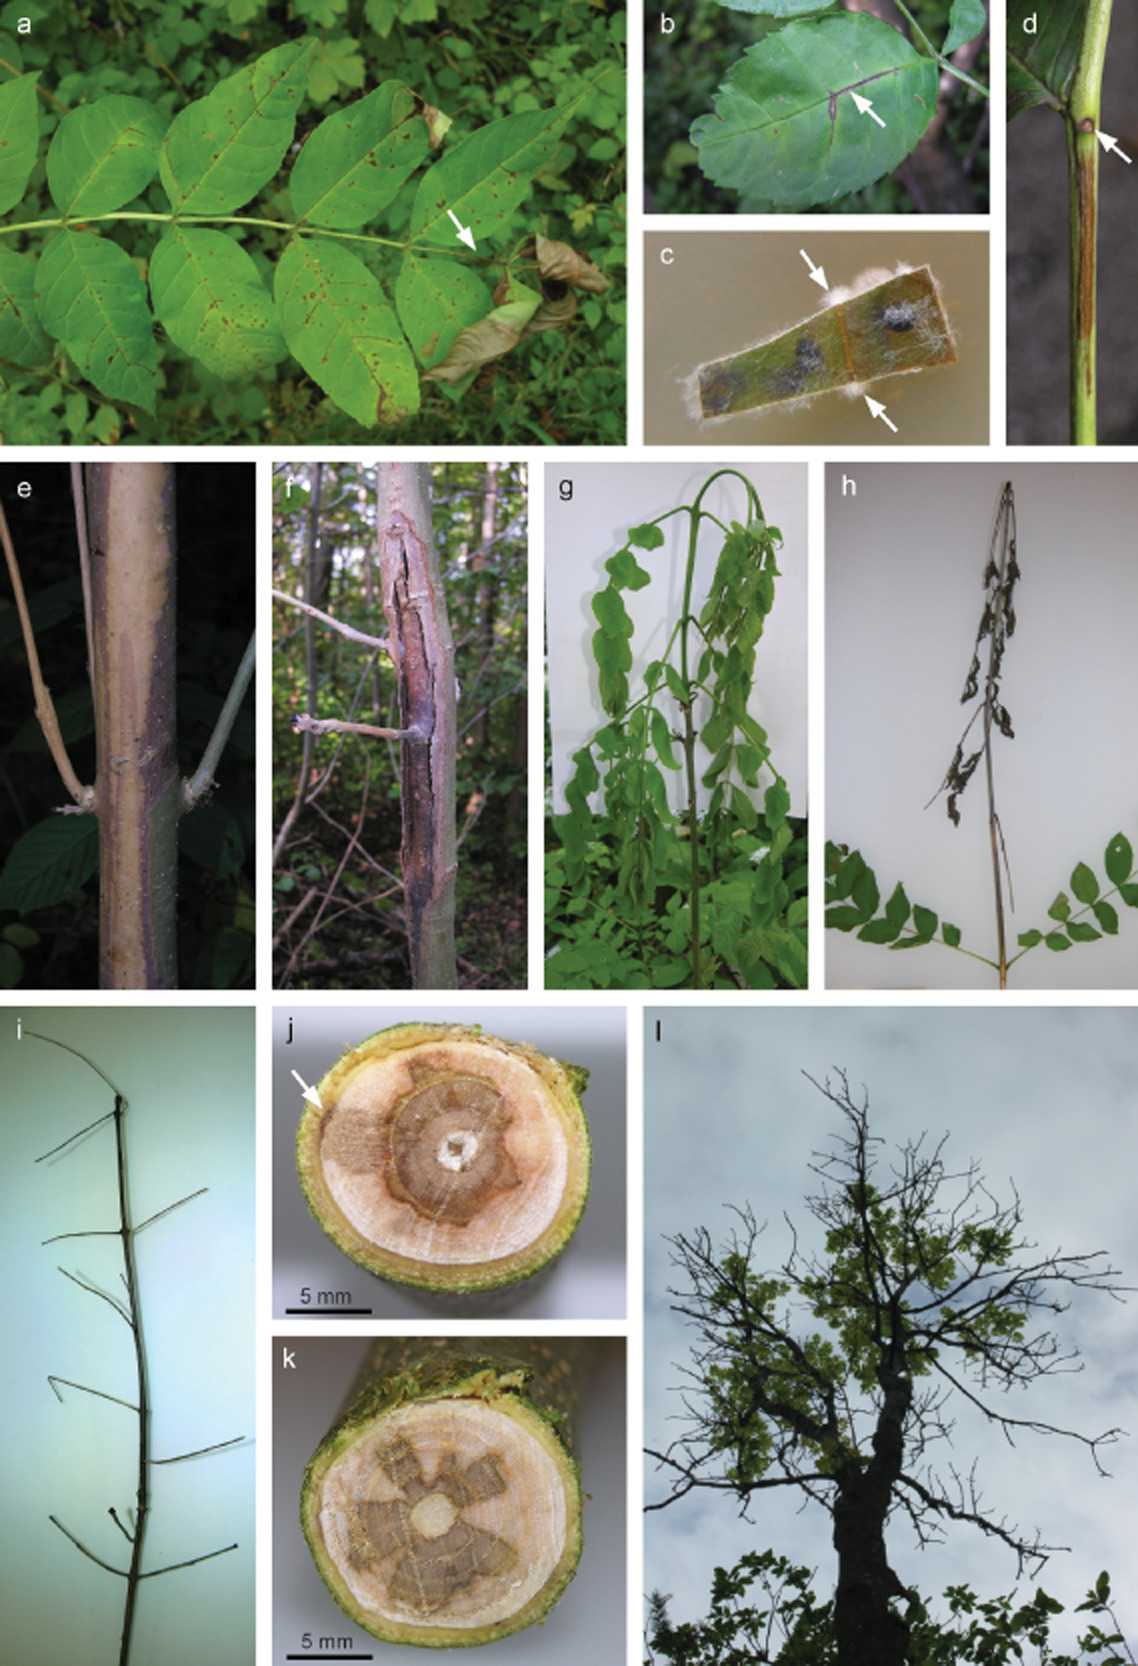
\includegraphics[scale=0.5]{chapter2/figures/gross2014.jpg}
    \caption{
    The symptoms of ash dieback, taken from the work of \cite{gross2014h}. 
    The pathogen \textit{H. fraxineus} infects the leaves of ash, leading to early onset wilting and desiccation. 
    The fungus then reproduces asexually, spreading through twigs, branches and eventually the xylem. 
    Symptoms include wilting, necrotic lesions, crown dieback and eventual mortality.}
    \label{fig:ash-deiback-symptoms}
\end{figure}

The pathogen HF is lethal to European ash (\textit{Fraxinus excelsior}) of all ages. 
Nevertheless, research has established that small young ash trees are more at risk,
and susceptibility declines with maturity. Surveys of ash stands conducted by \cite{marccais2017estimation} 
in Belgium recorded that after six years of infection, small young saplings died with $35\%$ mortality, 
whilst slightly larger ash ($<25 \mathrm{cm}$ in diameter) displayed mortality of $11\%$. 
In contrast only $3.2\%$ of large mature ash ($>25\mathrm{cm}$ in diameter) died.

Various sources of ash mortality data have been collected in different European countries;
in Germany, a forest stand of planted ash trees showed a $73\%$
mortality rate after five years \cite{langer2015ash} (as cited in a review
\cite{enderle2017ash}), while observations of ADB progression in Austria
suggest a low mortality rate of $5\%$ measured over a two-year window \cite{kessler2012dieback}. 
A study conducted at different sites throughout Great Britain suggests a time scale ranging between 
$3-15$ years of infected tree growth before death \cite{wylder2018evidence}.

In addition to age, ash survival also depends on the landscape. 
Landscape features and ADB progression were studied by \cite{https://doi.org/10.1111/1365-2745.13383} 
over a sample plot of size  $\mathrm{3.5km \times 6.5 km}$ in France; observations over two years
suggest that the surrounding landscape has little impact initially in $2012$. However, after pathogen establishment, 
later surveys in $2016$-$2018$ showed that landscape features play an essential role.
Among the results put forward by \cite{https://doi.org/10.1111/1365-2745.13383}, 
a highly abundant ash region increased the prevalence of collar canker and rachis symptoms in neighbouring ash.
In addition, the authors found that the influence of ADB decayed exponentially up to $200-300\mathrm{m}$ away from the high density source,
thus suggesting a density-dependency in ADB spread.

Modelling work suggests a myriad of environmental factors can also predict the
vulnerability of ash and subsequent spread of disease \cite{dal2014risk}.
Spatial regression analysis conducted by \cite{chumanova2019predicting} in the Czech Republic indicates that altitude 
is an important predictor of pathogen growth, which also support the strong negative temperature dependence observed by \cite{hauptman2013temperature}.

\subsection{Life cycle and reproductive mode}
% WIKI: Hymenoscyphus fraxineus has two phases to its life-cycle: sexual and asexual.[9] The asexual stage (anamorph) grows in affected trees attacking the bark and encircling twigs and branches.[9] The sexual, reproductive stage, (teleomorph) grows during summer on ash petioles in the previous year's fallen leaves.[7] The ascospores are produced in asci and are transmitted by wind; this might explain the rapid spread of the fungus.[

The reproductive mode is intricate, and HF can infect hosts through the soil,
water, and air \cite{gross2012reproductive}; 
although, the primary natural driver of disease propagation is through wind-dispersal
during summertime sporulation. Sporulation typically occurs from June-September when 
fungal fruiting bodies on the previous litter-fall release ascospores \cite{grosdidier2018tracking, hietala2013invasive}.
Multiple ascospores sources can infect the same leaf \cite{gross2012reproductive}. 
Though the primary natural driver is wind, infection (and re-infection) of ash are also thought to be possible 
through the soil-borne mechanisms \cite{fones2016role}, albeit with low frequency.

Ash dieback is highly seasonal \cite{bengtsson2014seasonal} and follows a complex, yearly polycyclic infection cycle.
Infected ash hosts will shed their leaves in the autumn, proceeded by fungal fruiting bodies growing on the dead leaf litter until summertime.
In summer, fruiting body spores are wind-dispersed and continue the cycle by producing new secondary infections\textemdash 
together, the life cycle and symptom expressions are illustrated in Figure \ref{fig:ash-deiback-symptoms}.
It is interesting to note the cyclic similarities between yearly ADB infection/re-infection and the seasonal
infections due to crop rotations, e.g. \cite{tankam2020modelling}. 
Notwithstanding that infected crop removal usually coincides with harvest time instead of infected ash survival that can span years.

The life cycle of the fungus HF can be understood to have two well-differentiated reproductive modes, 
sexual and asexual\textemdash a common trait of phyla Ascomycota, or ascomycetes fungi \cite{hawker2016physiology}.
Initially, asexual spores (conidia) were hypothesised to only increase genetic variance and act as spermatia \cite{gross2014h};
however \cite{fones2016role} called this into question, suggesting instead that asexual reproduction of the pathogen 
may play a role in driving the pathogen spread. Despite the potentially significant claim put forward by \cite{fones2016role},
it has gained seemingly little traction, and the role of asexual reproduction is still not fully understood.

\begin{figure}
    \centering
    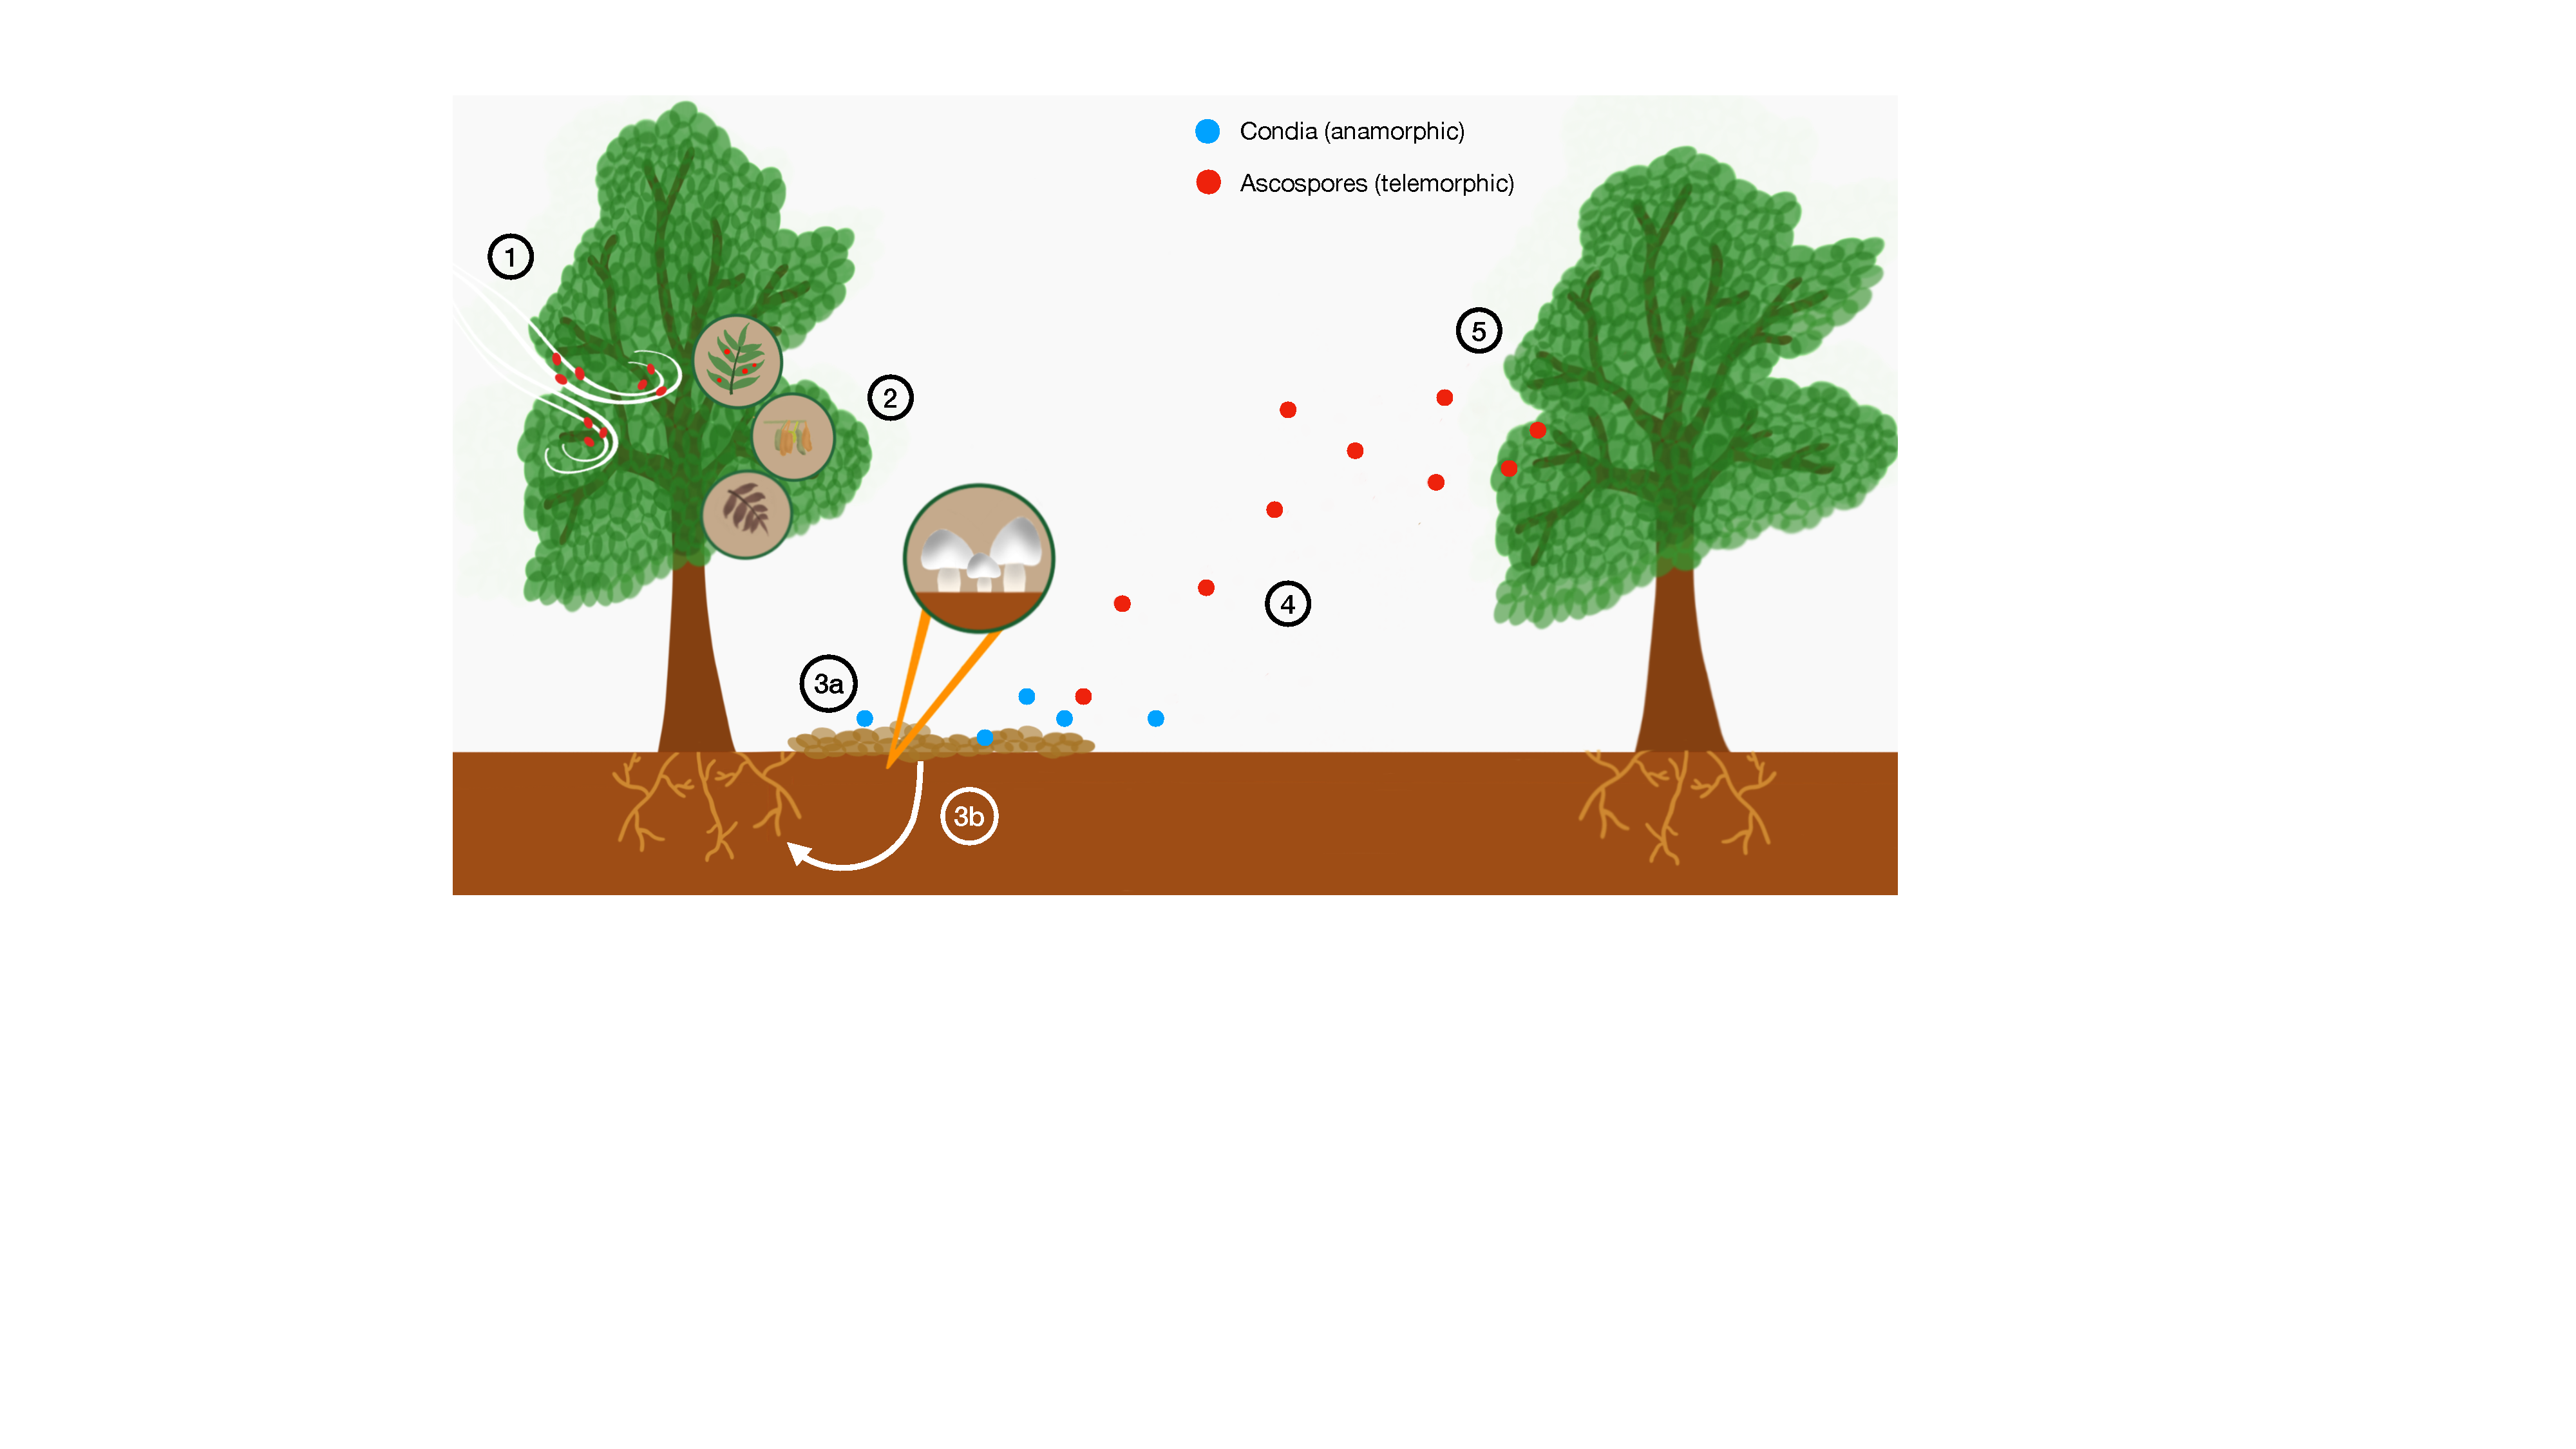
\includegraphics[scale=0.425]{chapter2/figures/ash-dieback-illustration.pdf}
    \caption{\textcolor{red}{describe ADB lifecycle} \blindtext }
    \label{fig:my_label}
\end{figure}

\newpage

\subsection{Dispersal}

In general, fungal spores have an efficient multi-scale wind-dispersal mechanism,
known to travel large distances \cite{golan2017long, wingen2013long, mundt2009aerial}
often described by power-law kernels, e.g. \cite{shaw2006assembling}.
From an epidemiological perspective, data on spore dispersal does not necessarily reflect the dynamics of new infections, 
as we cannot guarantee the availability of susceptible host material.
Even supposing available hosts, we cannot guarantee invasive spore colonisation.
However, studies on spore dispersal shed essential light on the spatial scale of ADB dispersal. 

Modern methods typically rely on `spore trapping' and real-time polymerase chain reaction (PRC) to study spores dispersal.
Data collected by \cite{chandelier2014detection} over three years using a (rotating arm) trapping system
and PRC amplification. The authors reported a $10\%$ spore trapping efficiency, and that most
dispersed ascospores remained within $50\mathrm{m}$ from the infectious source, with only a small number of spores exceeding 
distances beyond $50\mathrm{m}$. The work of \cite{chandelier2014detection} demonstrated the utility of novel PCR methods
to spore trap, but undesirably collected dispersal data over relatively small spatial scales.

Among the first landscape-scale fungal spore studies were conducted by \cite{long-range-dispersal}.
The authors focused on a comparable ascomycete fungus, \textit{Mycosphaerella fijiensis}, affecting banana plants.
Interestingly, \cite{long-range-dispersal} reported that asexual spore dispersal gradients extended 
a small distance $15\mathrm{m}$. As opposed to occasional, rare LDD in sexual (ascospore) dispersal up to $1000\mathrm{m}$.
Contrasting sexual and asexual spore dispersal was novel, and observing a small localised asexual dispersal gradient supports
the accepted idea that sexual dispersal in ADB is the dominant driver of disease spread.

Arguably the most comprehensive multi-scale study of ADB spore dispersal was performed by \cite{grosdidier2018tracking}.
In their paper, \cite{grosdidier2018tracking} tracked the local and landscape-level dispersal of ascospores
produced by \textit{H. fraxineus} in France.
The data collected relied on spore trapping and PRC; the reported trapping efficiency was $30–47\%$, marking an improvement over previous studies
e.g \cite{chandelier2014detection}. Most spores dispersal remained localised up to $50\mathrm{m}$ away from the inoculum source,
consistent with the results mentioned above put forward by \cite{chandelier2014detection}.
Nevertheless \cite{grosdidier2018tracking} set spore traps over much larger spatial scales ($\sim 100\mathrm{km}$),
subsequently detecting ADB spores $50-100\mathrm{km}$ ahead of the disease front.

Two dispersal kernels were used by \cite{grosdidier2018tracking}, a thin tailed Gaussian and an inverse 
power law of the forms:
\begin{equation}
    D(a, r) = \frac{1}{\pi a^2}\exp\big[-\frac{r^2}{a^2}\big]
    \label{eq:adb-ga}
\end{equation}
and
\begin{equation}
    D(a, r) = \frac{(b-1)(b-2)}{2\pi a^2}\big[ 1+ \frac{r}{a}\big]^{-b}
    \label{eq:geometric-invserse-power-law}
\end{equation}
where $a$ and $b$ are fitted parameters (for the Gaussian kernel, $a=\sqrt{2}\sigma$ with $\sigma$ being the standard deviation.). 
Equation \ref{eq:geometric-invserse-power-law} falls into the classical two-parameter geometric family of dispersal distributions.
The scale parameter is described by $a$ and the shape parameter by $b$. The mean dispersal distance described by Equation
\ref{eq:geometric-invserse-power-law} is  $\frac{2a}{b-3}$, and parameters $a$ and $b$ are valid for $a>0$ and $b>2$.

The functional form of Equation \ref{eq:geometric-invserse-power-law} is predicated on pollen dispersal studies,
as reviewed by \cite{nathan2012dispersal}. The tail of Equation \ref{eq:geometric-invserse-power-law} is 
particularly well suited to describe LDD events, as noted by \cite{https://doi.org/10.1111/j.1365-294X.2004.02100.x}
when describing the dispersal of pollen particulates. Moreover, a study by \cite{https://doi.org/10.1111/j.1365-294X.2006.03155.x}
used Equation \ref{eq:geometric-invserse-power-law} to model pollen-dispersal (and thus plant gene-flow) over landscape-level spatial scales. 
Presumably, the ability of Equation \ref{eq:geometric-invserse-power-law} to describe LDD, and the size similarity between pollen and fungi spores, 
motivated \cite{grosdidier2018tracking} to include it their field study. 
% A recent article published by \cite{golan2017long} presents an interesting system to 

\newpage

\subsection{Management and control}

Losing abundant ash populations could have dire consequences for several ecosystem functions, 
including nutrient recycling, food webs, and biodiversity.
As such, ADB presents a conservation challenge throughout Europe and Great Britain \cite{pautasso2013european}.
Moreover, under the rapid proliferation of ADB, various ash-dependent species risk extinction;
\cite{hultberg2020ash} identified $115$ at-risk (lichens, fungi, invertebrates, bryophytes/moss) species in Sweden that rely on ash.
Alarmingly, many of the ash-associated species identified by \cite{hultberg2020ash} also depend on elm species, which in turn face 
the fungal pathogen Dutch elm disease \cite{brasier1991ophiostoma}.

Given the ecological importance of ash in numerous temperate European forest types (e.g. floodplain, ravine, 
and lowland \cite{dobrowolska2011review}), management and pathogen control remain essential. The control of ash dieback
in a well-established focus of infestation, in both natural and artificial environments, is virtually impossible
\cite{havrdova2017environmental}, and it is already well recognised that ADB will eventually wipe out the vast 
majority of ash in Great Britain \cite{ash-dieback-costs}.

Controlling the spread of ash dieback reflects the spatial and temporal scale over which it spreads.
In particular, ADB fungal spores are thought to be able to jump between patches of ash,
even in the absence of susceptible hosts \cite{wingen2013long}.
However, LDD accounts for only a small minority of spore dispersal.
Furthermore, despite many notions of LDD, no unified LDD classification system exist, 
which led \cite{golan2017long} to propose a definition based on the distance traversed by the top $1\%$ of spores.

The long-term survival of ash depends on a small proportion of genetically resistant ash trees.
Despite many unpublished reports, genetic tolerance studies only began surfacing around a decade
after the widespread outbreak \cite{kjaer2012adaptive, stener2013clonal, mckinney2014ash}.
In particular, \cite{doi:10.1094/PHYTO-11-15-0284-R} showed the heritability of crown dieback and
collar-lesion symptom expression. In the three French provenances sampled,
\cite{doi:10.1094/PHYTO-11-15-0284-R} found no evidence for regional tolerance.
Presently, genetic tolerance is widely accepted \cite{havrdova2016differences, skovsgaard2017silvicultural},
and more recent work has focused on metabolomic tolerance classification,
profiling which metabolite markers correlate with resistance 
\cite{nemesio2020canditate, nemesio2020metabolomics, sidda2020diversity, chaudhary2020identification}.

A silvicultural system proposed by \cite{skovsgaard2017silvicultural} involves visually scoring severity based on crown dieback
and collar lesions. In this scheme, forest managers would inspect disease severity to record disease progression over time
and record genetically resistant trees to cultivate for future timber production. In addition, 
\cite{skovsgaard2017silvicultural} proposed that diseased forest stands should not be indiscriminately felled on account of high-value
tolerant individuals; this suggestion stands in contrast to the idea of a `cull radius', as alluded to by \cite{WEBIDEMICS}. 
In general, felling infected stands is ill-advised  \cite{chandelier2017ash}, except when infected hosts present a risk of uncontrolled 
and damaging tree-fall\textemdash as explained by \cite{ash-dieback-costs} when assessing the clean-up cost within Great Britain.

Following the establishment of genetic tolerance, numerous long-term preservation strategies 
rest on cultivating and replanting trees that exhibit low damage levels. Breeding 
programs in many European countries are currently underway, as reviewed by \cite{https://doi.org/10.1002/ppp3.10060}.
In the UK, the Living Tree Project (https://livingashproject.org.uk) aims to collate tolerant UK ash for future breeding.

% \cite{ash-tree2}
% - Approaches to conservation differ between forest and commercial ash stand \cite{skovsgaard2017silvicultural}. 
% - Among the control strategies, application of fungicide to infected biomass has been shown effective \cite{hauptman2015application}
% Among LDD human-mediated.
% - read me ->

% - statistical modelling work has shown the importance of environmental factors in the spread of disease \cite{dal2014risk, chumanova2019predicting}
% - the risk of spread.. was conduced by \cite{fellenor2019ash}....
% - \cite{dal2015epidemiology} un-published thesis

% % % % 3) The construction of the simple lattice model
% -----------------------------------------------------------------------------
% 1) Introduce toy percolation model
% 2) Include stochastic infectivity parameter
% 3) Show behaviour in one and two dimensions
% 4) Set the basis model and establish the main ensemble method 
% -----------------------------------------------------------------------------

\chapter{Tree disease: a simple lattice model}
\label{chapter:SLM}

Typically, models of tree disease are complicated and involve multiple parameters informed by experimental data. Moreover, modelling a specific pathosystem requires in-depth, specialist knowledge to incorporate biological realism, such as pathogen lifecycles or environmental suitability. This introductory chapter outlines a simple model of tree disease spreading through a forest that will lay the foundations for more detailed treatment in later chapters.
Consequently, the compartmentalised $SIR$, percolation-based, model used by \cite{OROZCOFUENTES201912} will be recounted. 

From the first principles, the percolation model will be analysed over one parameter, tree density $\rho$.
Thus, leading to a mathematical and conceptual definition of percolation in the context of tree-based epidemics. 
The simple one-parameter model will then give way to a discussion of criticality and self-similarity in the system;
the discussion will include a summary of critical phenomena and some universal behaviour within the model.
Crucially, this chapter demonstrates the importance of thresholds in the spread of tree-based diseases.

Having established a simple one-parameter model, a more involved two-parameter `stochastic percolation' model will be developed and examined. 
Stochastic percolation will include an extra parameter representing the degree of pathogen infectivity. 
In general, measuring infectivity is challenging and subject to much spatial and temporal variation, such as changing climatic/environment conditions or species-level genetic variations in susceptibilities.  
However, including a stochastic infectivity parameter is essential to construct representative models of tree-based epidemics, as infectivity (or susceptibility) can vary widely over a landscape.
The two-parameter model will constitute a simple lattice model (SLM) of disease dynamics. 
This introductory chapter will introduce an ensemble-averaging method used throughout the thesis;
in the present case, ensemble-averaged parameter sweeps are used to categorize the SLM behaviour.

\section{Percolation formalism}
% understand universality class and scaling exponents 
% we consider small timescales and neglect regrowth factors
Consider a square lattice of size $L \times L$ , where each site in the lattice can be in one of two states: %
open with probability $\rho$ or closed with probability ($1-\rho$). %
Therefore, the probability $\rho$ describes a density parameter and encapsulates the occupancy of a homogeneous distribution of open and closed lattice positions.
One open site ($c_p$) is connected to another ($c_q$) if laid within the Von Neumann neighbourhood \cite{toffoli1987cellular}.

A connected set of open nearest neighbours define a cluster denoted by $C$, where $c_i \in C$.
Given the set $C$, it is possible to traverse between member sites $c_i \in C$ by moving through the lattice in either horizontal or vertical steps `Von Neumann motion'. 
Given two distinct non-overlapping clusters $c_i \in C_1$ and $c_j \in C_2$, then $c_i \neq c_j $ i.e. there is no way to jump from $C_1$ to $C_2$ following Von Neumann motion. 
Connectivity is defined between lattice sites rather than the edges which connect them, known as `site' percolation\textemdash as opposed to `bond' percolation.

If $\rho$ is close to zero, only small clusters would be present as a disordered system; 
conversely, if $\rho$ is large, a connected network of open positions would dominate the domain, thus defining an ordered system.
At some point for $\rho \in [0, 1]$, a critical threshold ($\rho_c$) would be reached, and a singularity of connected sites would span an infinite sized lattice.
On a finite lattice, the cluster is said to percolate and form a `spanning cluster' ($C_\infty$) that extends between at least two different edges of the lattice.
The formation of the spanning cluster occurs abruptly between a very narrow range of $\rho$ values. 
Therefore, the threshold for percolation defines a critical-point \cite{STAUFFER19791}. 

The critical point can be defined as the least value of $\rho$ where percolation occurs with non-zero probability. %
This can be formalised by first considering the probability function: $\theta (\rho)= \lbrace \rho:|C|=\infty\rbrace$ where $\theta(\rho)$ is the probability of an arbitrary site, %
within a lattice of density $\rho$, belonging to cluster $C$ of size $\infty$ (i.e. the spanning cluster). %
The critical value then satisfies: %

\begin{equation}
\label{eq:critical_threshold_1d}
    \rho _{c}=sup \lbrace \rho : \theta (\rho ) = 0 \rbrace
\end{equation}

At this point, the spanning cluster has been described conceptually, although many nuances and technicalities complicate the definition. %
For example, the probability of percolation has a non-trivial dependence on the size of the lattice;
if the mean cluster size, defined by a `characteristic' cluster length $C_r$, is above or comparable to $L$, 
percolation could occur despite the density residing in the sub-critical regime. %
The size of the lattice is therefore required to be sufficiently large compared to individual lattice positions (or microscopic interactions) 
in order to approximate the threshold ($\rho_c$) reliably and produce a spanning cluster ($C_{\infty}$). 

When the domain size is large, the threshold $\rho_c$ will remains approximately constant and insensitive to small changes in the domain. 
All proceeding simulations in this chapter are conducted on finite-sized domains between two and three orders of magnitude larger than individual lattice points.
The model presented in this chapter (first published by \cite{OROZCOFUENTES201912}) was 
found to agree with the accepted percolation threshold, when the lattice had size $L \sim 500\times500$;
the lattice configuration used here will therefore assume the same size configuration. 

Intuitively, it is clear to see the link between percolation and epidemiology: 
open lattice positions act as susceptible members of a population ($S$), and $\rho$ defines a density of the hosts. 
In this paradigm, the spanning cluster describes a high-impact epidemic that spreads uncontrollably. 
Small to medium-sized clusters existing at (or slightly below) the threshold describe short-lived, 
failed epidemics where the pathogen spreads for a time before becoming extinct.

These analogies have clear limitations when describing mobile hosts, but fortunately, trees are sessile and immobile.
Thus, percolation theory provides a valuable framework for modelling tree diseases (see Chapter \ref{section:lit-rev-perc} 
for a review of percolation-based models). 
Forming a percolation-based lattice model of tree disease requires us first to combine a compartmental $SIR$-like model within the lattice ($L$) mentioned above. %
Next, an appropriate transmission dynamic is described to model the spread of disease between lattice points.


\section{Percolation-based $SIR$}

The percolation density parameter ($\rho$) defines a simple host distribution.
Namely, $\rho$ represents the probability of a susceptible tree $S$ (given a numerical value $1$), 
while empty lattice positions define an insusceptible state $\emptyset$ (with numerical value $0$).
If a susceptible tree neighbours an infected tree, it will transition into the $I$ compartment (having a numerical value of $2$).
Transitions between states occur with a probability of 1, and the Von-Neumann neighbourhood describes the connectivity between trees.
After an arbitrary number of time-steps $T$, an infected tree will transition into the removed state $R$ and die; 
see appendix \ref{a:propagation} for more information on the numerical implementation. %
For simplicity, the infectious lifetime will not be considered as a parameter but will remain fixed at $T=1.0$\textemdash revisited below in section \ref{ch3:two-param-model}.

The initial conditions begin with a small patch of infected hosts (of size $5\times5$) located at the origin ($L_O$) at $t=0$, and percolation events describe the boundary conditions. 
Percolation occurs when the infection spreads from $L_O$ to any of the four lattice boundaries;  thus defining a connected cluster of infectious-removed that spans the domain from $L_O$.
Each time-step through the simulation represents an arbitrary unit of time, and simulation termination occurs on one of three boundary conditions: 
1) a percolation is observed 
2) the pathogen becomes extinction 
3) a time-horizon of $N$ steps is reached. 
Typical simulations on a domain of size $500 \times 500$ are shown in Figure \ref{fig:ch3-perc-spread} through three time-steps. 

\begin{figure}
    \centering
    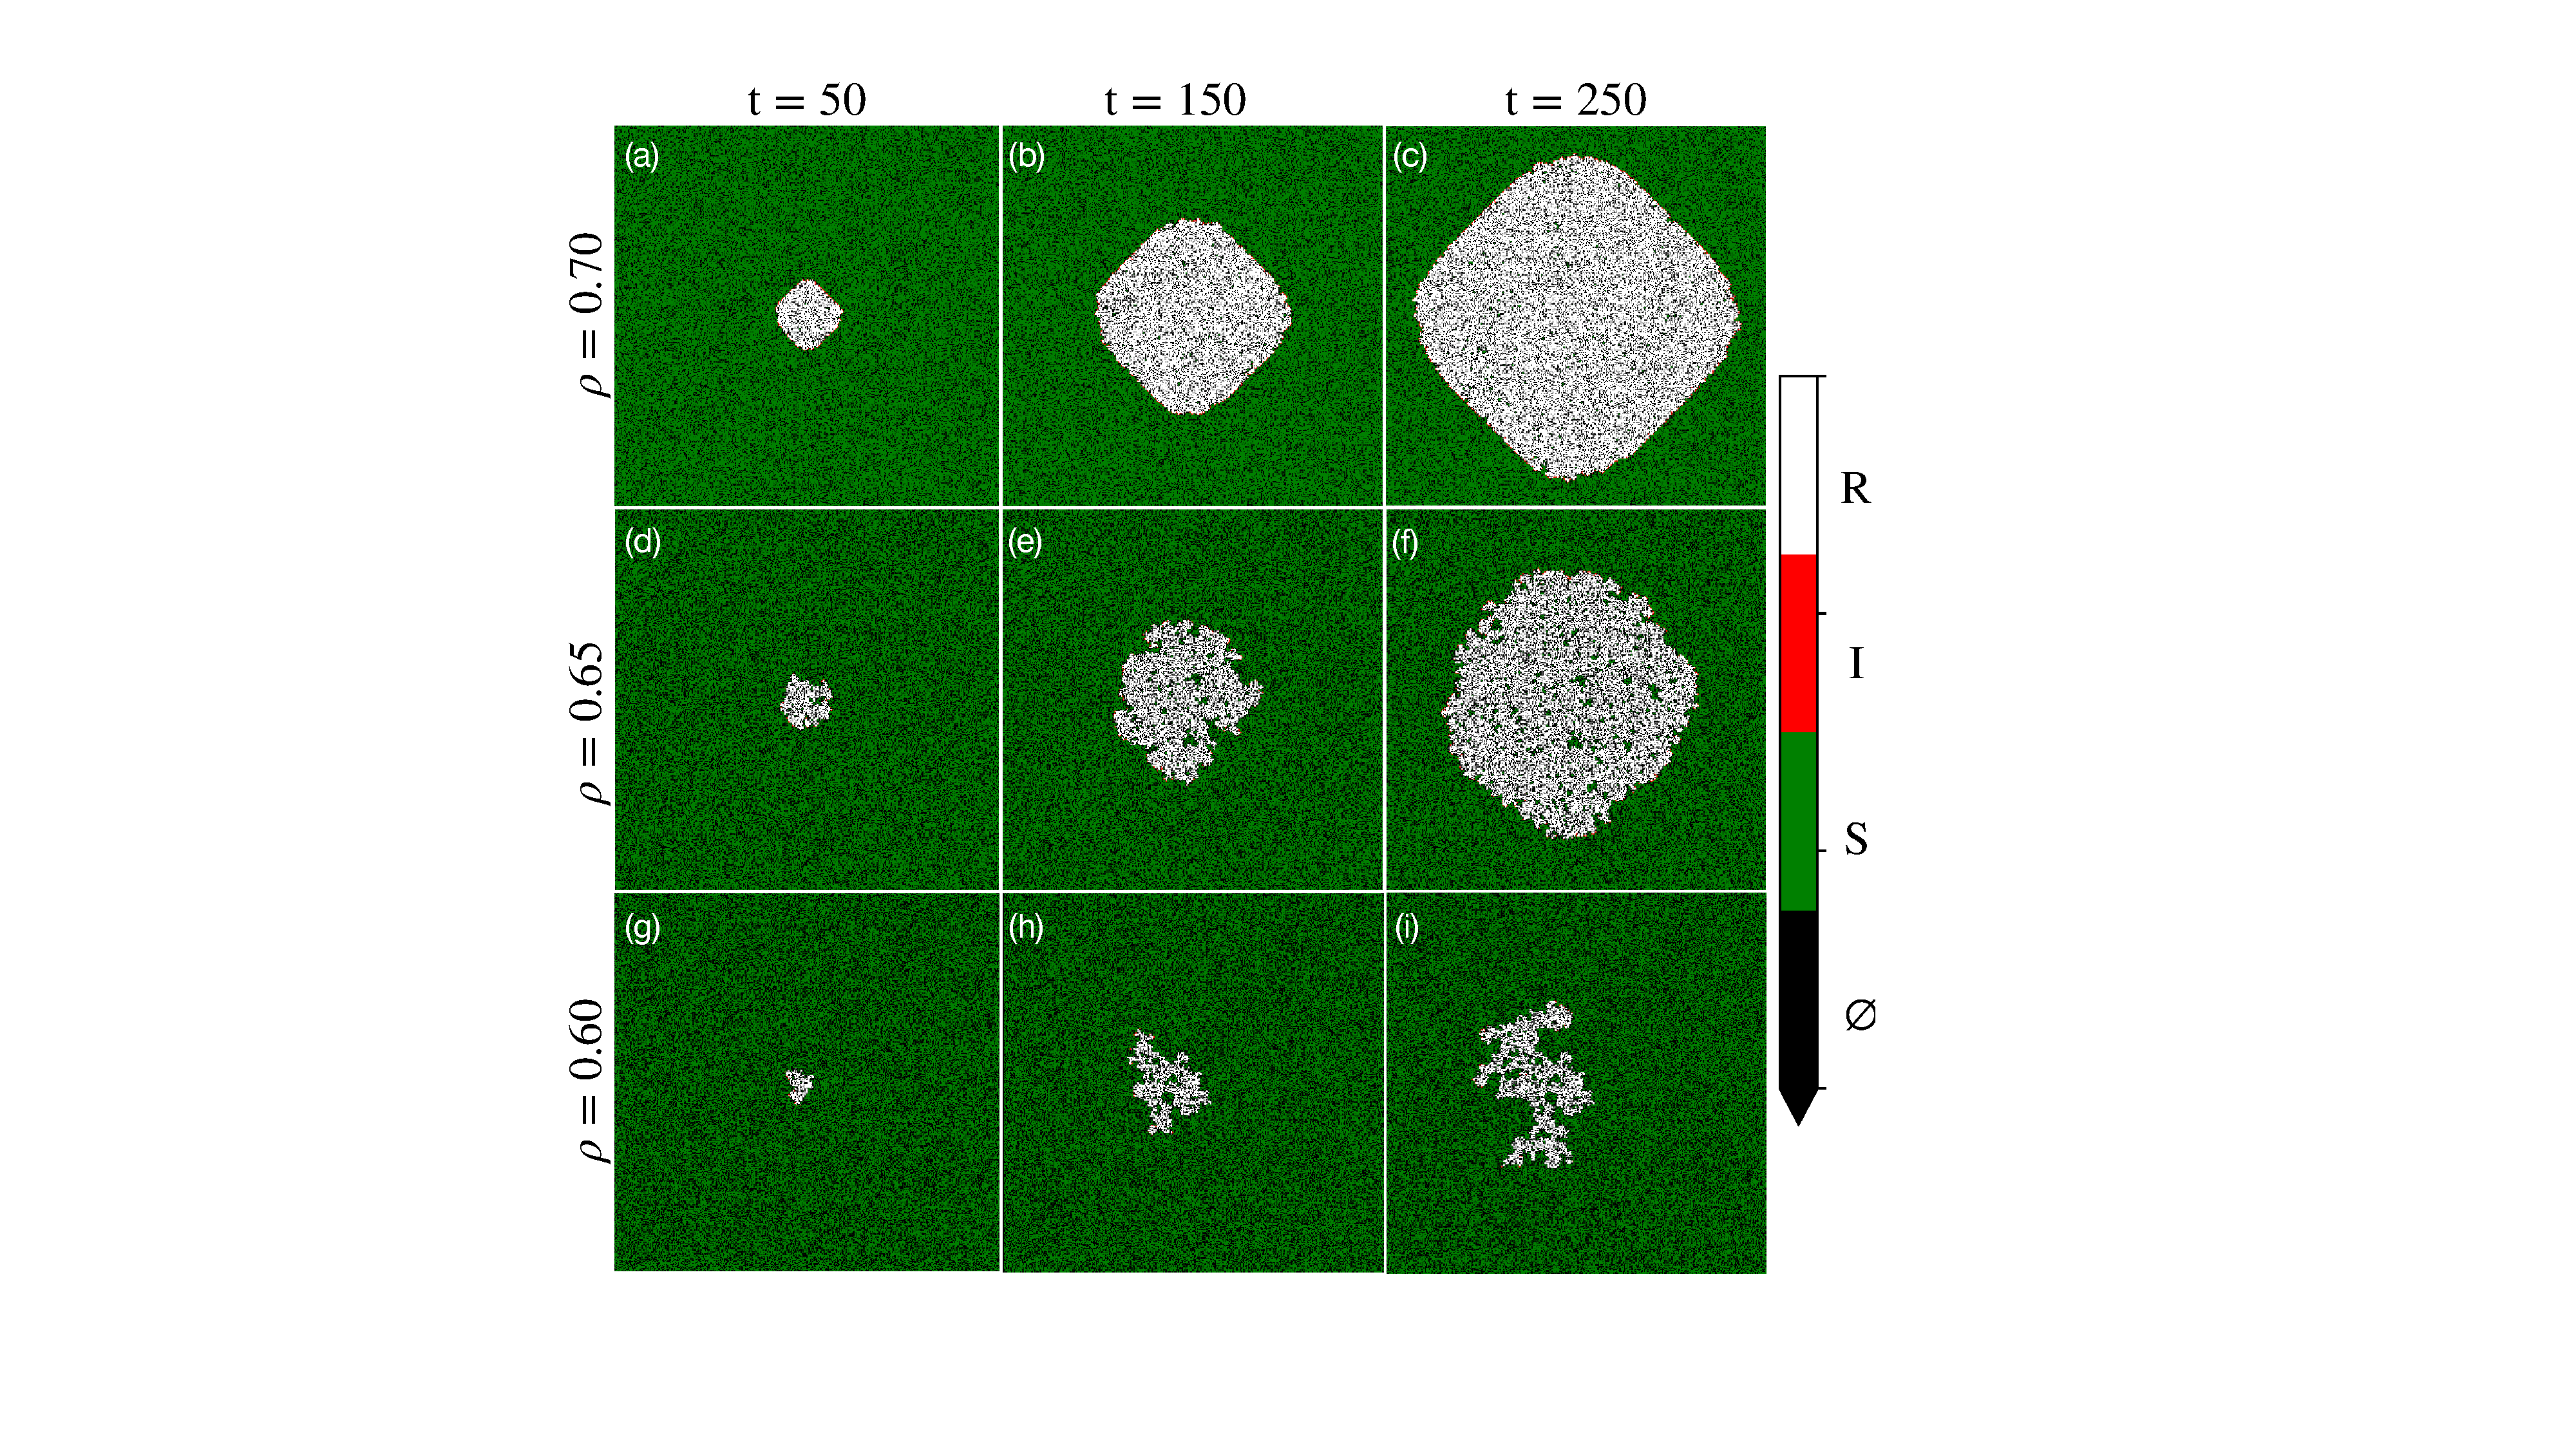
\includegraphics[scale=0.50]{chapter3/figures/figure1-1param-perc.pdf}
    \caption{
        Evolving outbreaks in the one-parameter, percolation-based $SIR$ model are shown for different tree densities ($\rho$).
        From left to right, three successive time-steps are plotted on a domains of size $500 \times 500$.
        Green and black pixels represent susceptible and insusceptible (empty) host units, respectively, 
        while white and red lattice sites depict removed and infectious hosts. 
        (a-c) High-density simulations reveal an unnatural diamond-shaped spread, undesirably reflecting the underlying lattice geometry.
        (d-f) Simulations above the threshold spread radially outward from the epicentre, defining a connected cluster of infectious-removed trees in the process. (g-i) Around the percolation threshold, the disease spreads slowly and chaotically outward. 
        }
    \label{fig:ch3-perc-spread}
\end{figure}

Figure \ref{fig:ch3-perc-spread} illustrates dynamic simulations of disease spread through a 
series of $500 \times 500 $ domain. At density $\rho=0.70$, Figures \ref{fig:ch3-perc-spread} (a-c)
reveal an unnatural diamond-like pattern of spread reflecting artefacts of the lattice geometry.
In theory, the diamond-like spread would look different if the lattice geometry is changed\textemdash a
triangular or honeycomb lattice, for example. The diamond-like spread begins to disappear in 
Figure \ref{fig:ch3-perc-spread}(d-f), when simulations have density $\rho=0.65$.
At this density, a wave-like propagation of infected trees spread radially from the epicentre outward 
toward the lattice boundary and look more realistic.
Interestingly, these observations can be understood through the lens of stochasticity. At a lower tree density, the probability of 
spread between neighbours is lower, and the spread is more chaotic, thus disrupting the highly ordered wavefront shown 
through panels (a-c) into a circular travelling wavefront.

Figure \ref{fig:ch3-perc-spread}(g-i), show the spread of disease for a lower host density of $\rho = 0.60$.
As the disease spreads outward, a more fractal-like pattern begins to emerge.
Moreover, the disease spreads slowly, as evidenced by the smaller area traced by the infectious-removed trees shown from white to red.
In this regime of spread, `persisting' simulations result from the slowly evolving epidemic as it defines a disordered cluster of infectious-removed hosts.
\newpage

\subsection{Percolation threshold}
\label{section:universality}

Suppose simulations begin at low density, below the threshold; in this case, evolving epidemics are unlikely to percolate to the domain boundary, and the pathogen will become extinct.
If the host density increases, we can imagine that epidemics begin percolating to the boundary for some specific value.
Consequently, the probability of percolation was examined over a sweep of density parameters, shown in Figure \ref{fig:ch3-perc}(a).
Unsurprisingly, a threshold-like behaviour is revealed.
All the simulations that form Figure \ref{fig:ch3-perc}(a) evolved inside a $500\times 500$ sized domain.
The probability of percolation ($Pr(\rho)$) defines
a critical region, highlighted in orange (where $ \rho \in [0.57, 0.62$]), that separates regimes of pathogen extinction and percolation/epidemic.
The threshold depicted by Figure \ref{fig:ch3-perc}(a) is consistent with the accepted percolation threshold for a two-dimensional square $\rho_c \approx 0.592$.

The value of $Pr(\rho)$ depends non-trivially on stochasticity, which motivated an ensemble-averaged approach\textemdash 
further reading on the underlying theory of ensemble-averaging can be found in \cite{gibbs1902elementary}.
In Figure \ref{fig:ch3-perc}(a), 100 repeated simulations obtain the probability of percolation. Simulations that percolate to the domain boundary assume the numerical value of one, while pathogen extinction events assume zero; for each value of $\rho$, the average value is computed, thus defining a probability $Pr(\rho)$.

At the critical density, denoted by $\rho_c$, we witness the emergence of some exciting phenomena.
Figures \ref{fig:ch3-perc}(c-d) show a spanning cluster ($C_\infty$) of infectious and removed trees (in white to red respectively) at $\rho_c=0.592$.
The cluster looks remarkably similar at all spatial resolutions, said to be `self-similar' \cite{Kapitulnik_1983}.
Within $C_\infty$, one can identify clusters of untouched susceptible trees (in green) of various sizes, suggesting a distribution of cluster sizes occupy all possible length scales.
In the literature, clusters can be described by a `cluster number' ($n_s$) distribution, where $n_s$ is the number of clusters containing $s$ open/susceptible lattice sites.
Furthermore, around the percolation threshold, there can be significant fluctuations in the size of the clusters formed\footnote{
The related statistical fluctuations analysed by \cite{OROZCOFUENTES201912}
present an effective early warning system for the prediction of forest-based pathosystems\textemdash revisited in the next chapter.
}.

\begin{figure}
    \centering
    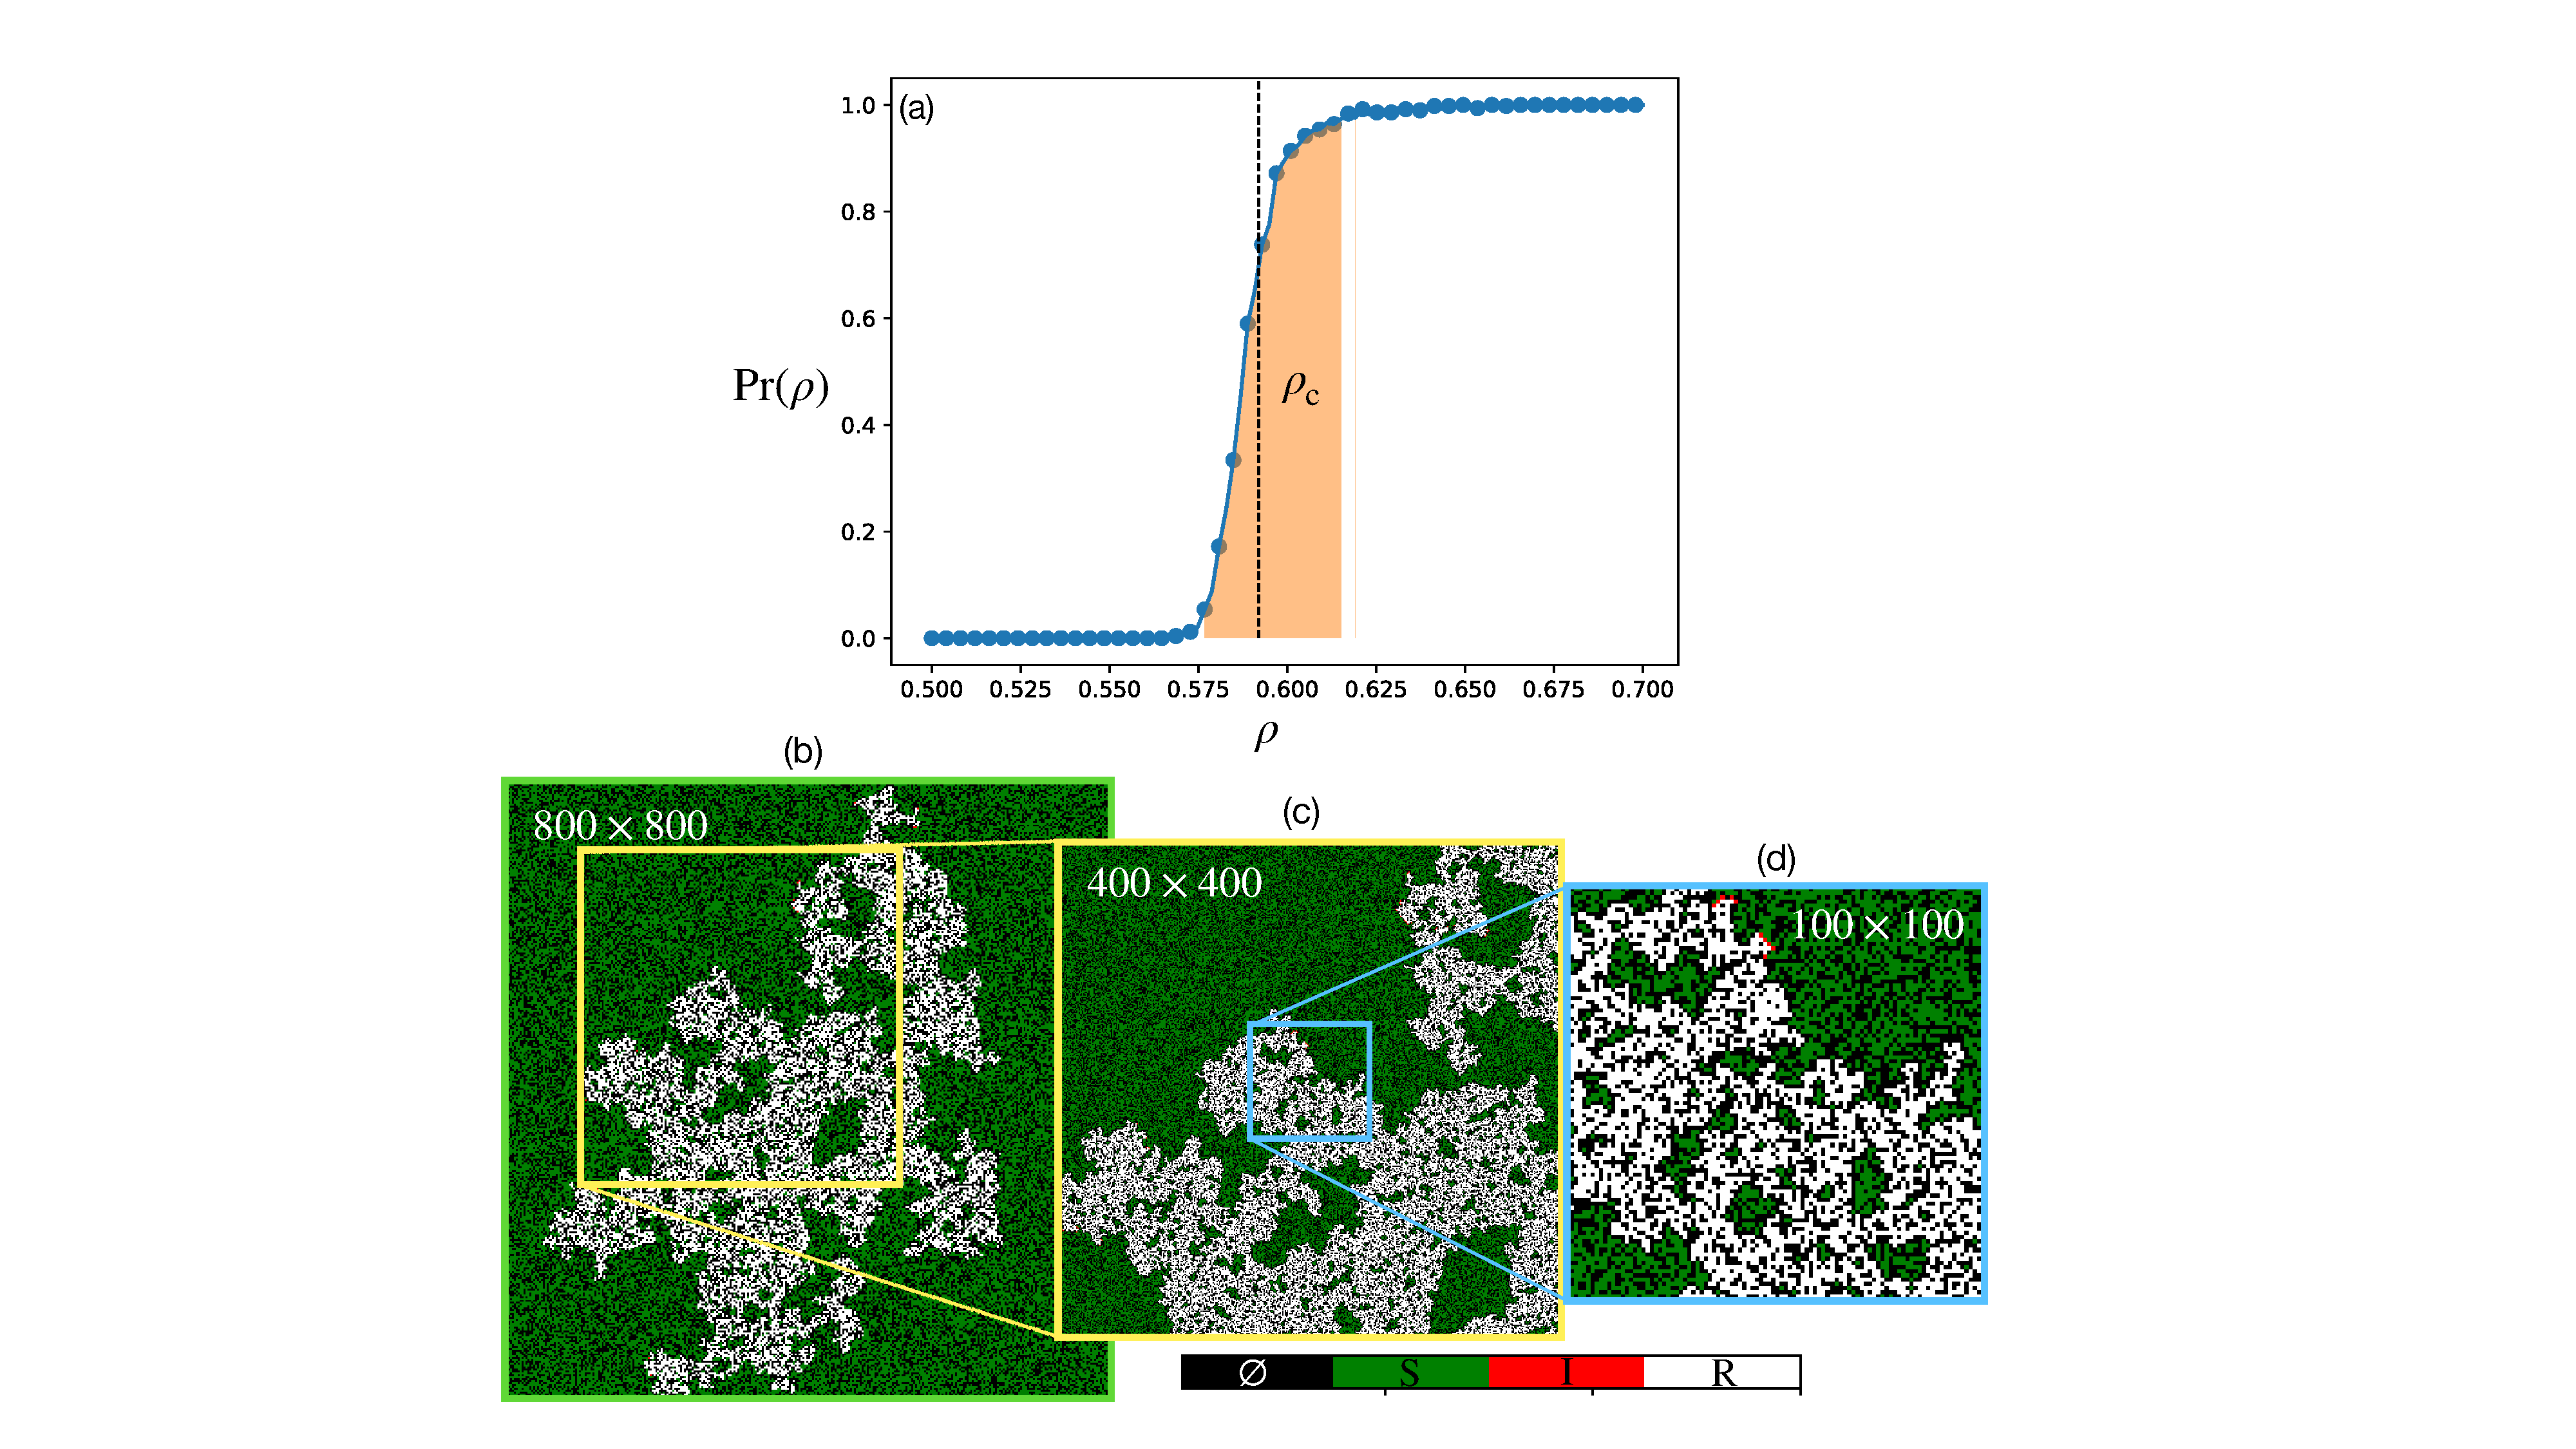
\includegraphics[scale=0.4]{chapter3/figures/figure2-1param-perc-threshold.pdf}
    \caption{The percolation threshold is determined for the one-parameter percolation $SIR$ model.
            (a) The probability of percolation ($\mathrm{Pr(\rho)}$) is plotted against host density.
            The shaped orange region highlights a threshold consistent with results from classical percolation theory, 
            namely $\rho_c = 0.592$, shown by the vertical dashed line. 
            (b-c) At the critical density $\rho_c$, a cluster spanning the domain in (b) is assessed over progressively smaller resolutions.
            Similar features are observed on different scales and scale invariance is observed in the model.
            }
    \label{fig:ch3-perc} % \label{fig:ch3-perc-pr}
\end{figure}

\begin{table}[h!]
  \begin{center}
    \begin{tabular}{l|c|c|r} % <-- Alignments: 1st column left, 2nd middle and 3rd right, with vertical lines in between
    \hline
      \textbf{Lattice} & NN & \textbf{Site percolation} & \textbf{Bond percolation}\\
      \hline
      1D & 2 & 1 & 1\\
      Square 2D & 4 & 0.593 & $1/2$\\
      Triangular 2D & 6 & $1/2$ & 0.347\\
      Honeycomb & 3 & 0.696 & 0.653\\
      Diamond & 4 & 0.43 & 0.388\\
      Voronoi & - & 0.714 & 0.667\\
    \hline
    \end{tabular}
    \caption{The site and bond percolation threshold for various lattice types\textemdash data published by \cite{stauffer2018introduction, PhysRevE.80.041101}.
            Each lattice configuration defines a set of nearest neighbours (NN).
    }
    \label{tab:perc}
  \end{center}
\end{table}

This chapter rests on a square lattice, although we could have considered many other configurations, e.g. a triangular, honeycomb or Voronoi lattice.
From the observation of Figures \ref{fig:ch3-perc-spread}(a-c),
high host densities would produce highly ordered wavefronts reflecting the different lattice configurations.
In addition, various quantities within the model would change, especially the critical density $\rho_c$ that changes in response to the nearest neighbour (NN) number.
For completeness, table \ref{tab:perc} shows a selection of site and bond percolation thresholds.
Even though $\rho_c$ would change between lattice configurations, some universal properties of the model would remain fixed, 
which leads to a description of universality below.


\subsection{Universality}

At $\rho \sim \rho_c$, percolation and scaling theory explain how the system follows a power law of the form $\propto (\rho - \rho_c)^{\alpha}$ 
where $\alpha$ is a universal critical exponent.
All systems that possess the same exponent are members of the same `universality class' \cite{PhysRev.180.594, RevModPhys.76.663}.
Consider the probability that one open site (at the origin) is connected to another open site a distance $r$ away. %
In this scenario, the probability is described by the `correlation function' $g(r)$. %
The behaviour of this function defines a length scale, denoted as the `correlation length' $\xi$ that dictates how the probability of `connectedness' decays with distance $r$. %
For densities close to percolation threshold: %
\begin{equation}
    \xi \sim |\rho - \rho_c|^{-\nu}
    \label{eq:universal-scaling}
\end{equation}
where $\nu$ is a critical exponent that is universal for all lattice configurations and only depends on the dimension of the lattice used. In general, there are critical exponents for other quantities, e.g. cluster sizes\textemdash discussed more below. 
However, all follow similar power laws, as shown by \cite{stauffer2018introduction, STAUFFER19791}.

Equation \ref{eq:universal-scaling} can be understood by exploring how the connectivity of open sites depend on the density and the divergence that occurs at the threshold $\rho=\rho_c$. 
For low densities, $\xi$ is small because all clusters exist in singlets/triplets.
However, as $\rho$ increases, the mean cluster length increases as more sites become open and connect to form larger clusters. 
As we approach the critical density (from the direction $\rho \rightarrow \rho_c^{-}$) the spanning cluster is formed and $\xi$ diverges towards infinity, $\xi \rightarrow \infty$. 
If one neglects the divergent spanning cluster, a similar picture is painted for densities just above criticality $\rho > \rho_c$. 
That is, the correlation length $\xi$ decays rapidly as $|\rho - \rho_c|$ increases. 
This time however,  mid-to-large sized clusters get absorbed by $C_\infty$ as the density increases;
thus leaving only small untouched clusters, as $\rho \rightarrow 1$ and $\xi \rightarrow 0 $. 
See \cite{STAUFFER19791} for a detailed breakdown of power laws and correlation length.

Lastly, it is worth discussing well-known results on how the cluster sizes (or masses) scale with the lattice dimension. 
If $\rho > \rho_c$, the largest cluster present (denoted by $M$) would scale according to $M\propto L^{2}$, cf. the evolving epidemics above the threshold in Figure \ref{fig:ch3-perc}; 
in contrast, if $\rho = \rho_c$, $M$ would follow $M\propto L^{1.9}$, 
where $d_F=1.9$ describes the cluster fractal dimension.
If we normalise the cluster by the size of the lattice ($L^2$), the mean density of $M$ will decay as the lattice size increases, i.e. $L^{1.9}/L^2 = L^{-0.10}$. 
Broadly, the critical phenomena found in percolation theory, thermodynamics and magnetism have close ties and are described by similar power laws underpinned by scaling theory \cite{Essam_1980}.

% If the system crosses the percolation threshold, it can be likened to a phase-transition. %
% Subsequently, the terms `phase-transition' and `percolation' will be used interchangeably throughout this work. 


\section{Pathogen infectivity}
\label{ch3:two-param-model}

We have established a percolation-based model of tree disease described by a one-dimensional parameter-space over tree density $\rho$. %
We now extend the parameter-space to include an `infectivity' parameter, denoted by $\beta$. %
Previously, we made an implicit assumption about pathogen-transmission, namely: 
infected trees will transmit the infection to susceptible nearest neighbours with perfect fidelity, that is, a probability of $1$. 
In reality, a pathogen may display a range of virulence depending on the environmental suitability or host susceptibility; 
exemplified by the pathogen ash dieback, known to cause more host damage in naturally occurring forest ecosystems \cite{marciulyniene2017can} 
and release more fungal spores conditional on temperature \cite{chandelier2014detection}.

To model infectivity, the parameter $\beta$ is introduced. The probability of a susceptible tree becoming infected during a single time-step is given by: $Pr(S \rightarrow I) = \beta$. Appendix \ref{a:propagation} contains more descriptive information on the computational implementation. 
The infectivity parameter describes a transmission `rate' (i.e. per time-step) and is closely linked to the infectious lifetime $T$ of the tree. %
If a susceptible host falls within a von Neuman neighbourhood of an infected host, it will remain susceptible with probability:
\begin{equation}
\label{eq:pr_s_s}
    Pr(S \rightarrow S) = \rho(1 -\beta)^T
\end{equation}
where $T$ is the number of an infectious lifetime;
thus, the probability of remaining susceptible decreases as the infectious lifetime gets larger.
Equation (\ref{eq:pr_s_s}) sets the scene for a predictive mean-field theory.
Subsequently, appendix \ref{a:slm-mean-field-theory} outlines steps toward a novel continuum model of tree disease.


Previously in the one-parameter $SIR$ variant, the infectious lifetime played a minor role in determining wavefront because pathogen transmission occurs with a probability of one.
However, now a susceptible host will survive for $t=T$ time-steps before transitioning into $R$. Ultimately, the model is non-dimensionalised, and the value of $T$ is arbitrary; however, a single step can be envisioned to be on the order of years.
At this stage, we have recovered the two-parameter model used by \cite{OROZCOFUENTES201912}, henceforth referred to as the `\textit{simple lattice model'} (SLM). 

Figure \ref{fig:slm} show three SLM simulations, spreading for the shown infectivity parameters through different time-steps.
All simulations in Figure \ref{fig:slm} are governed by a fixed value of $T=10$, and density $\rho=0.70$.
The colour bar in Figure \ref{fig:slm} represents different steps through the infectious period, from yellow to red.
Higher values of $\beta$ yield a faster spreading velocity,
as expected.
Figures \ref{fig:slm}(g-i) allude to $\beta$ altering the percolation threshold, on the basis of $\beta=0.25$ reflecting a more fractal-like spreading pattern, even well beyond the standard percolation threshold of $\rho_c=0.592$.

% Link  \cite{gilligan2008epidemiological} to the critical point

Figure \ref{fig:slm-wave-front} shows how variations in the infection lifetime can change the wave-front properties. 
The value of $\beta$ predominantly controls the speed of the wave-front, whereas $T$ controls the lag-time on the removal front. 
Therefore, increasing $T$ yields an increase in the wave-front thickness;
this is valid for $\rho > \rho_c$.
Around the percolation threshold $\rho \sim \rho_c$, the relationship between $T$ and spreading velocity is less obvious. 
Close to the percolation threshold, variations in $T$ have more importance, as it could lower or raise pathogen transmission below or above percolation thresholds, respectively.
If $T$ is held fixed, the critical threshold definition can now be generalised from Equation (\ref{eq:critical_threshold_1d}), to include the parameter $\beta$: 

\begin{equation}
\label{eq:critical_threshold_1d}
    \rho _{c}=sup \lbrace \rho, \beta : \theta (\rho, \beta ) = 0 \rbrace
\end{equation}

\begin{figure}
    \centering
    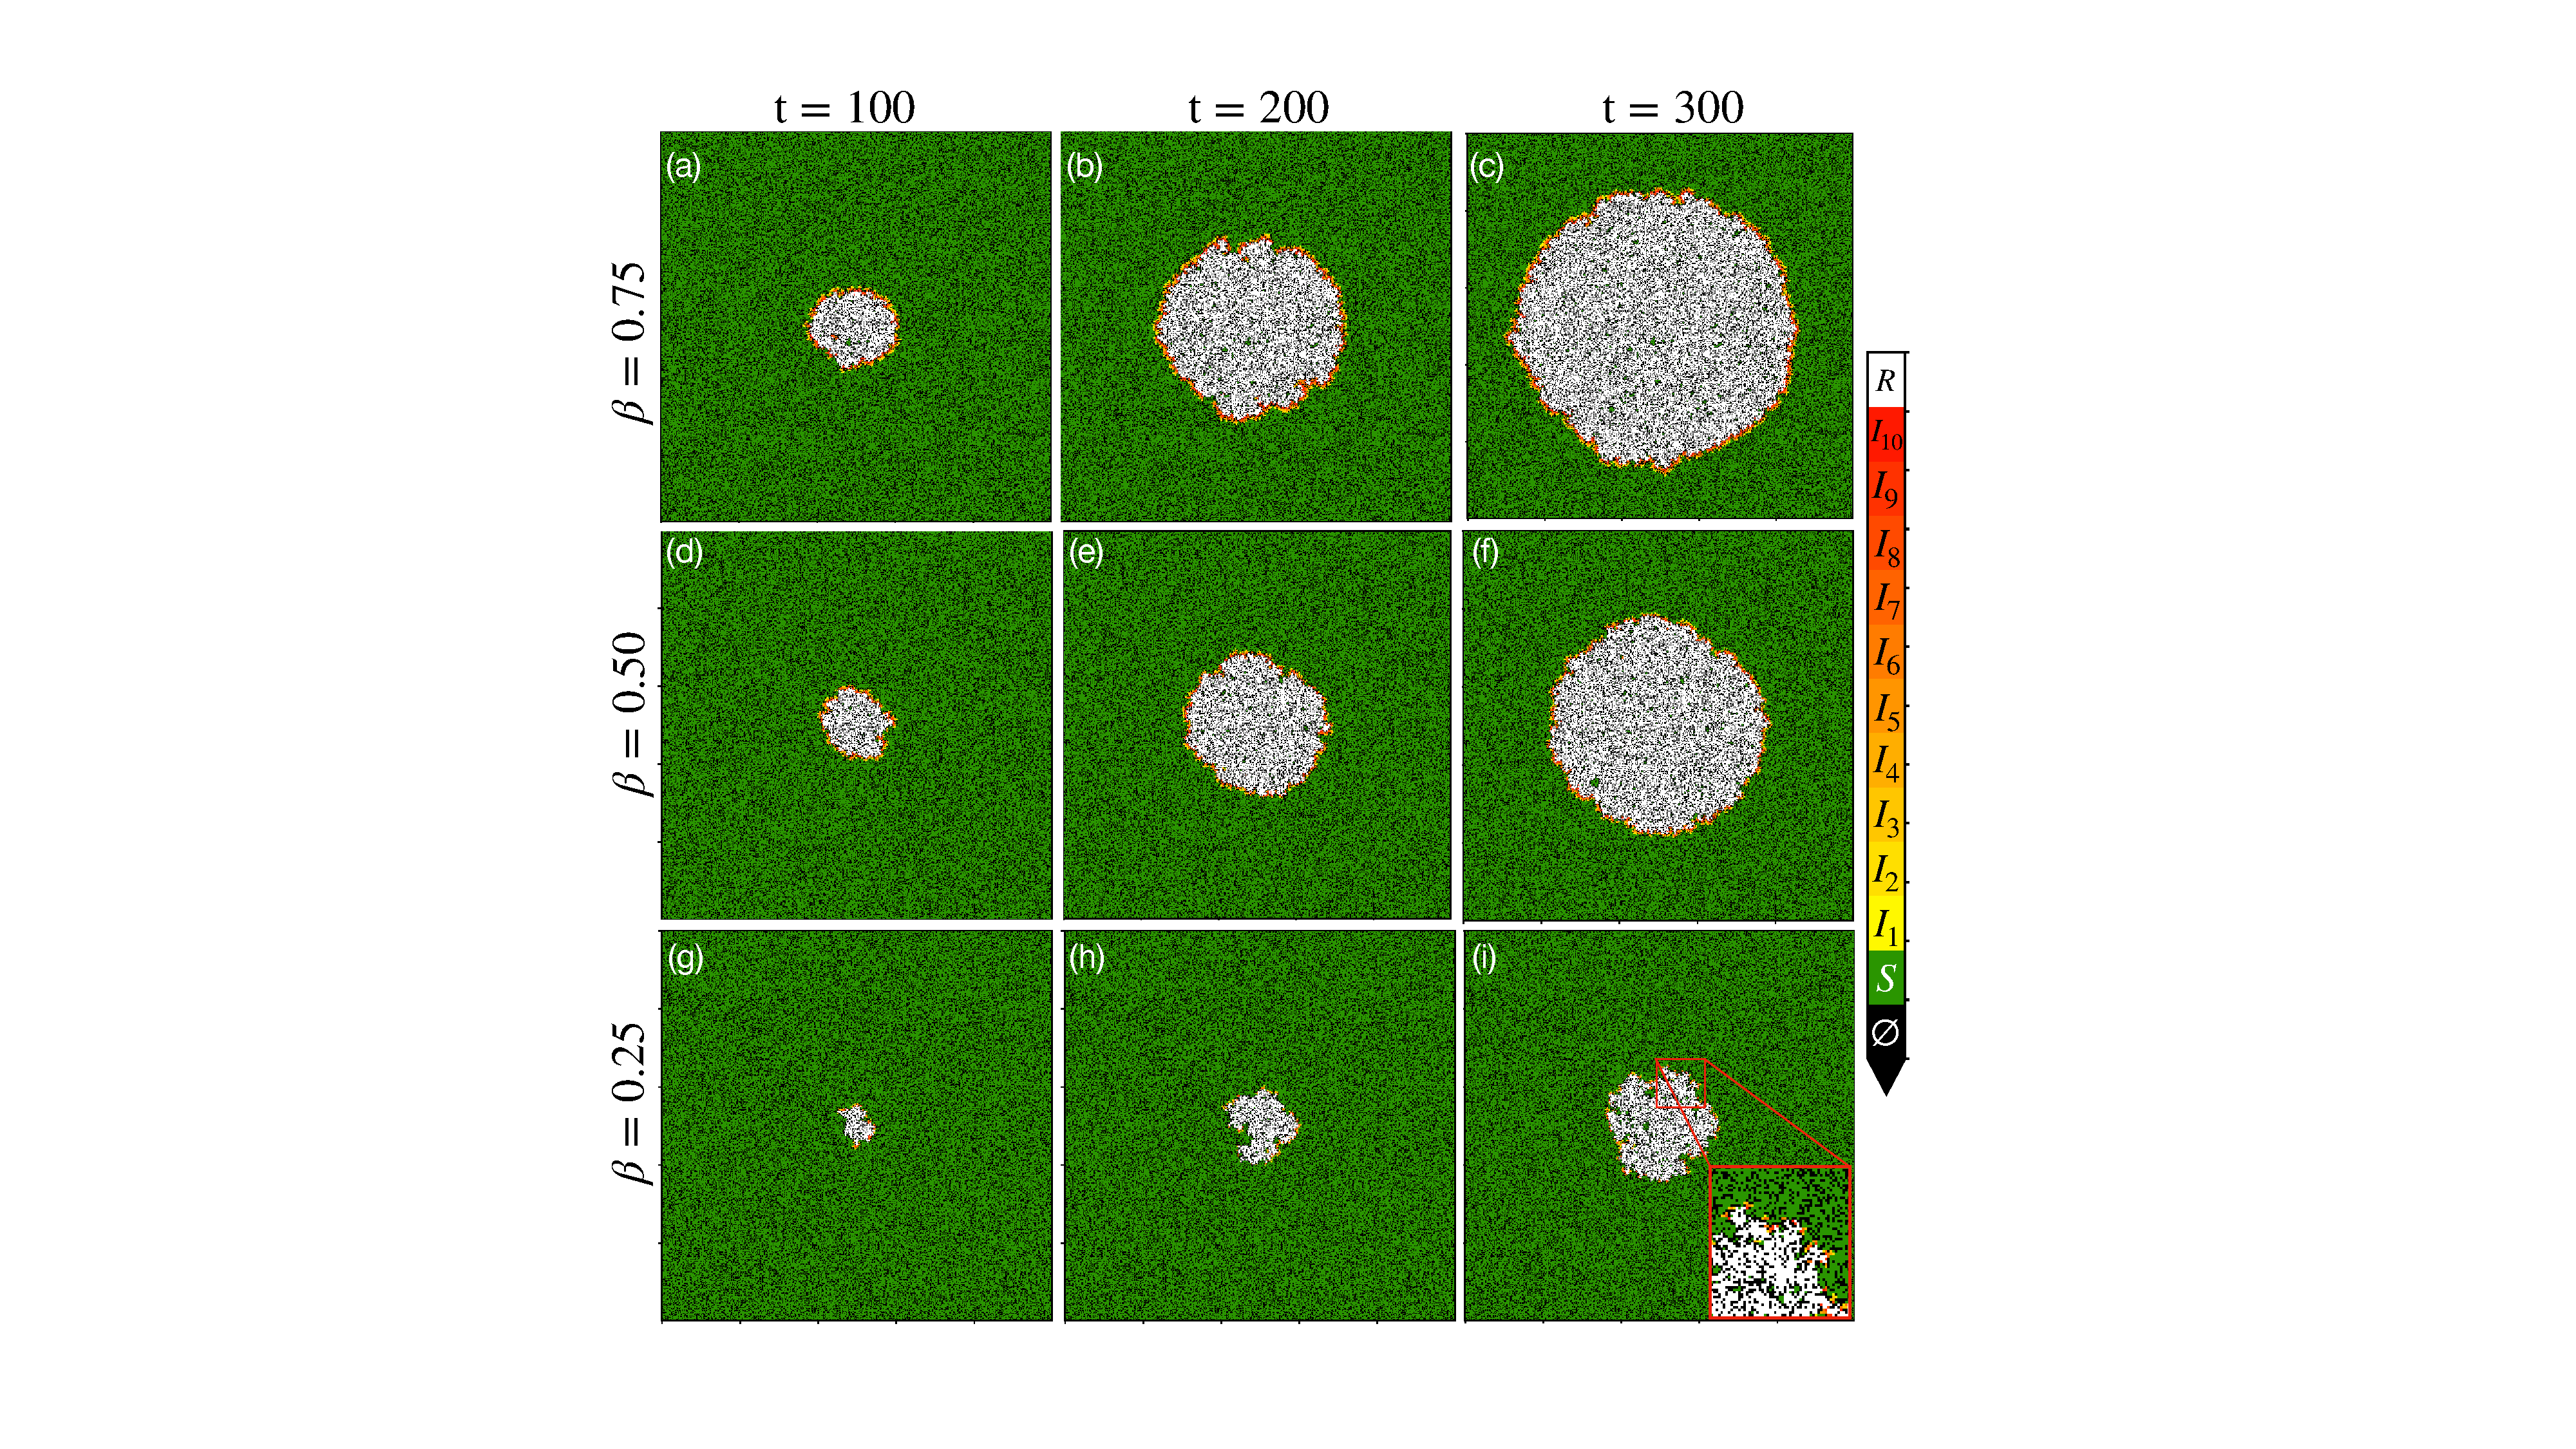
\includegraphics[scale=0.45]{chapter3/figures/figure3-two-param-model.pdf}
    \caption{Introducing an infectivity parameter $\beta$. The SLM is shown running on a domain of size $500\times500$ for fixed $T=10$ and density $\rho=0.70$. Simulation reveal that $\beta$ has an impact on the wave-front speed and changes the percolation threshold.}
    \label{fig:slm}
\end{figure}

\begin{figure}
    \centering
    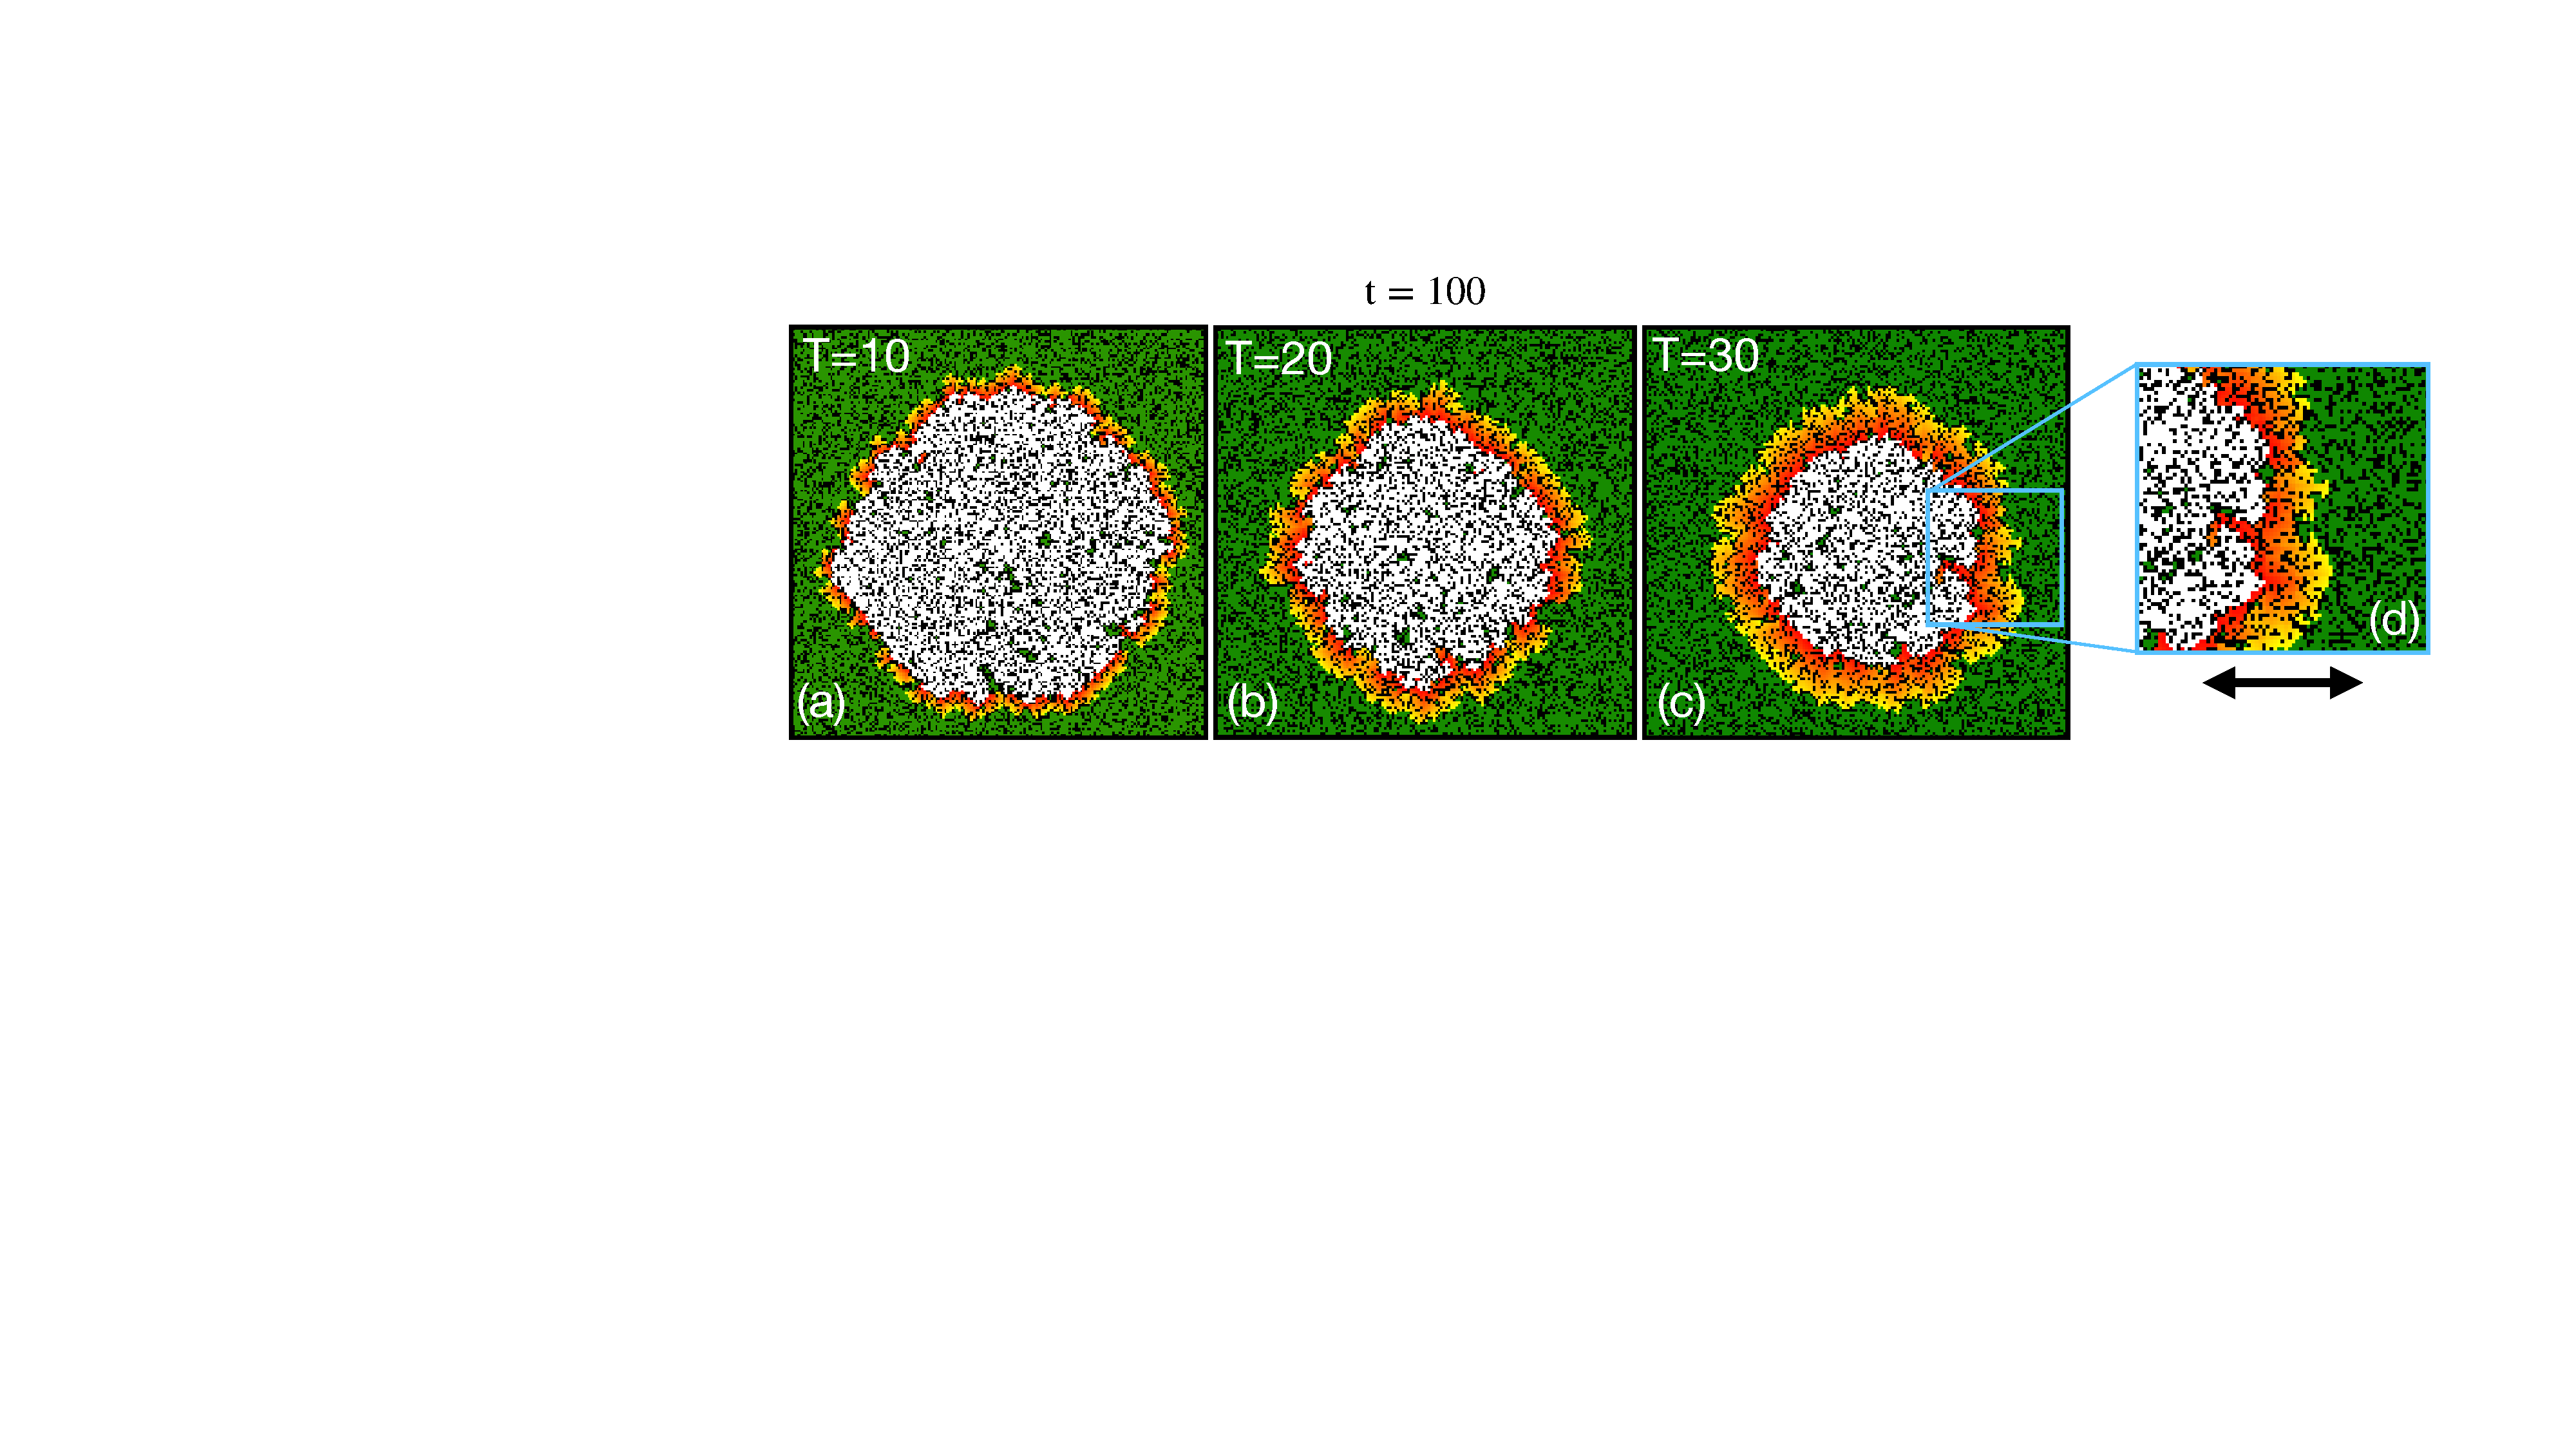
\includegraphics[scale=0.35]{chapter3/figures/figure5_.pdf}
    \caption{Simulations through a single time-step for fixed density and infectivity reveal that $T$ has little impact on the speed of the wave-front. 
    However, increasing $T$ leads to a thicker wavefront, as the posterior interface (between $R$ and $I$) lags behind the evolving wave-front (between $S$ and $I$).}
    \label{fig:slm-wave-front}
\end{figure}

\newpage

\section{Epidemic thresholds}
\label{sec:SLM-epidemic-threshold}

Previously in section \ref{section:universality}, the percolation probability was examined over one parameter of host density.
A threshold occurred over a narrow range of densities and separated the regime of epidemic and pathogen extinction.
Notwithstanding, we did not examine the rate of pathogen propagation nor any additional dynamic information.
In order to capture spreading rates, a metric comprising the `spreading velocity' is introduced, captured by: 
\begin{equation}
\label{eq:vel_eff_r}
    v_{radial(t)}=\sqrt{N_I(t+1)-N_I(t)}
\end{equation} 
where, $N_I$ is the number of infected trees in the domain at time-step $t$. 
The difference in $N_I$ between time-steps gives an `effective' radial velocity. %
The number of spatial units progressed by the pathogen is averaged over all angles per unit time. %
Strictly speaking, Equation (\ref{eq:vel_eff_r}) is valid only for $\rho > \rho_c$; at the percolation threshold, the wave-front assumes a fractal dimension and averaging over two dimensions becomes unreasonable.

The time-series, $v_{radial}(t)$ is shown in Figure \ref{fig:vel_eff_rad_metric}(a) for three combinations of $(\rho, \beta)$.
Unsurprisingly, higher-valued combinations produce a higher velocity.
Additionally, initial instability is most significant through the first $\sim 200$ time-steps, a consequence of the initial conditions which suggests the system has yet to reach a steady state.
Here, the system is said to be in a transient state.
In Figure \ref{fig:vel_eff_rad_metric}(a), a simulation average $\overline{v}_{radial}(t)$, 
can be determined and plotted as a horizontal line, repeating the measurement multiple times over an `ensemble', gives a probability distribution. 

Figures \ref{fig:vel_eff_rad_metric}(b-d) display the probability density functions\footnote{
To reduce artefacts of initial transience, any simulation that became extinct before the initial transient period 
of $t_{tr}\approx 200$, was excluded from calculations of the ensemble mean.} of the mean velocities.
In all panels, the vertical black line inside each distribution depicts the ensemble mean velocity.
For higher host densities, the mean velocity increases and distributions appear somewhat narrower.
Additionally, Figures \ref{fig:vel_eff_rad_metric}(b-d) suggest that $\beta$ plays a role in determining the velocity variance, as the distributions become wider with lower infectivity, cf. the green and blue distributions.

For now, the important statistic is merely the ensemble mean, denoted by $\big\langle\overline{v}\big\rangle$.
although, from Figures \ref{fig:vel_eff_rad_metric}(b-d), we can begin to access the third-order statistical moment of skew.
Namely, the green distributions become progressively right-skewed as density is lowered.
Statistical measures over the ensemble have exciting applications and can detect an early warning signal, a topic covered in the next chapter.

\begin{figure}
    \centering
    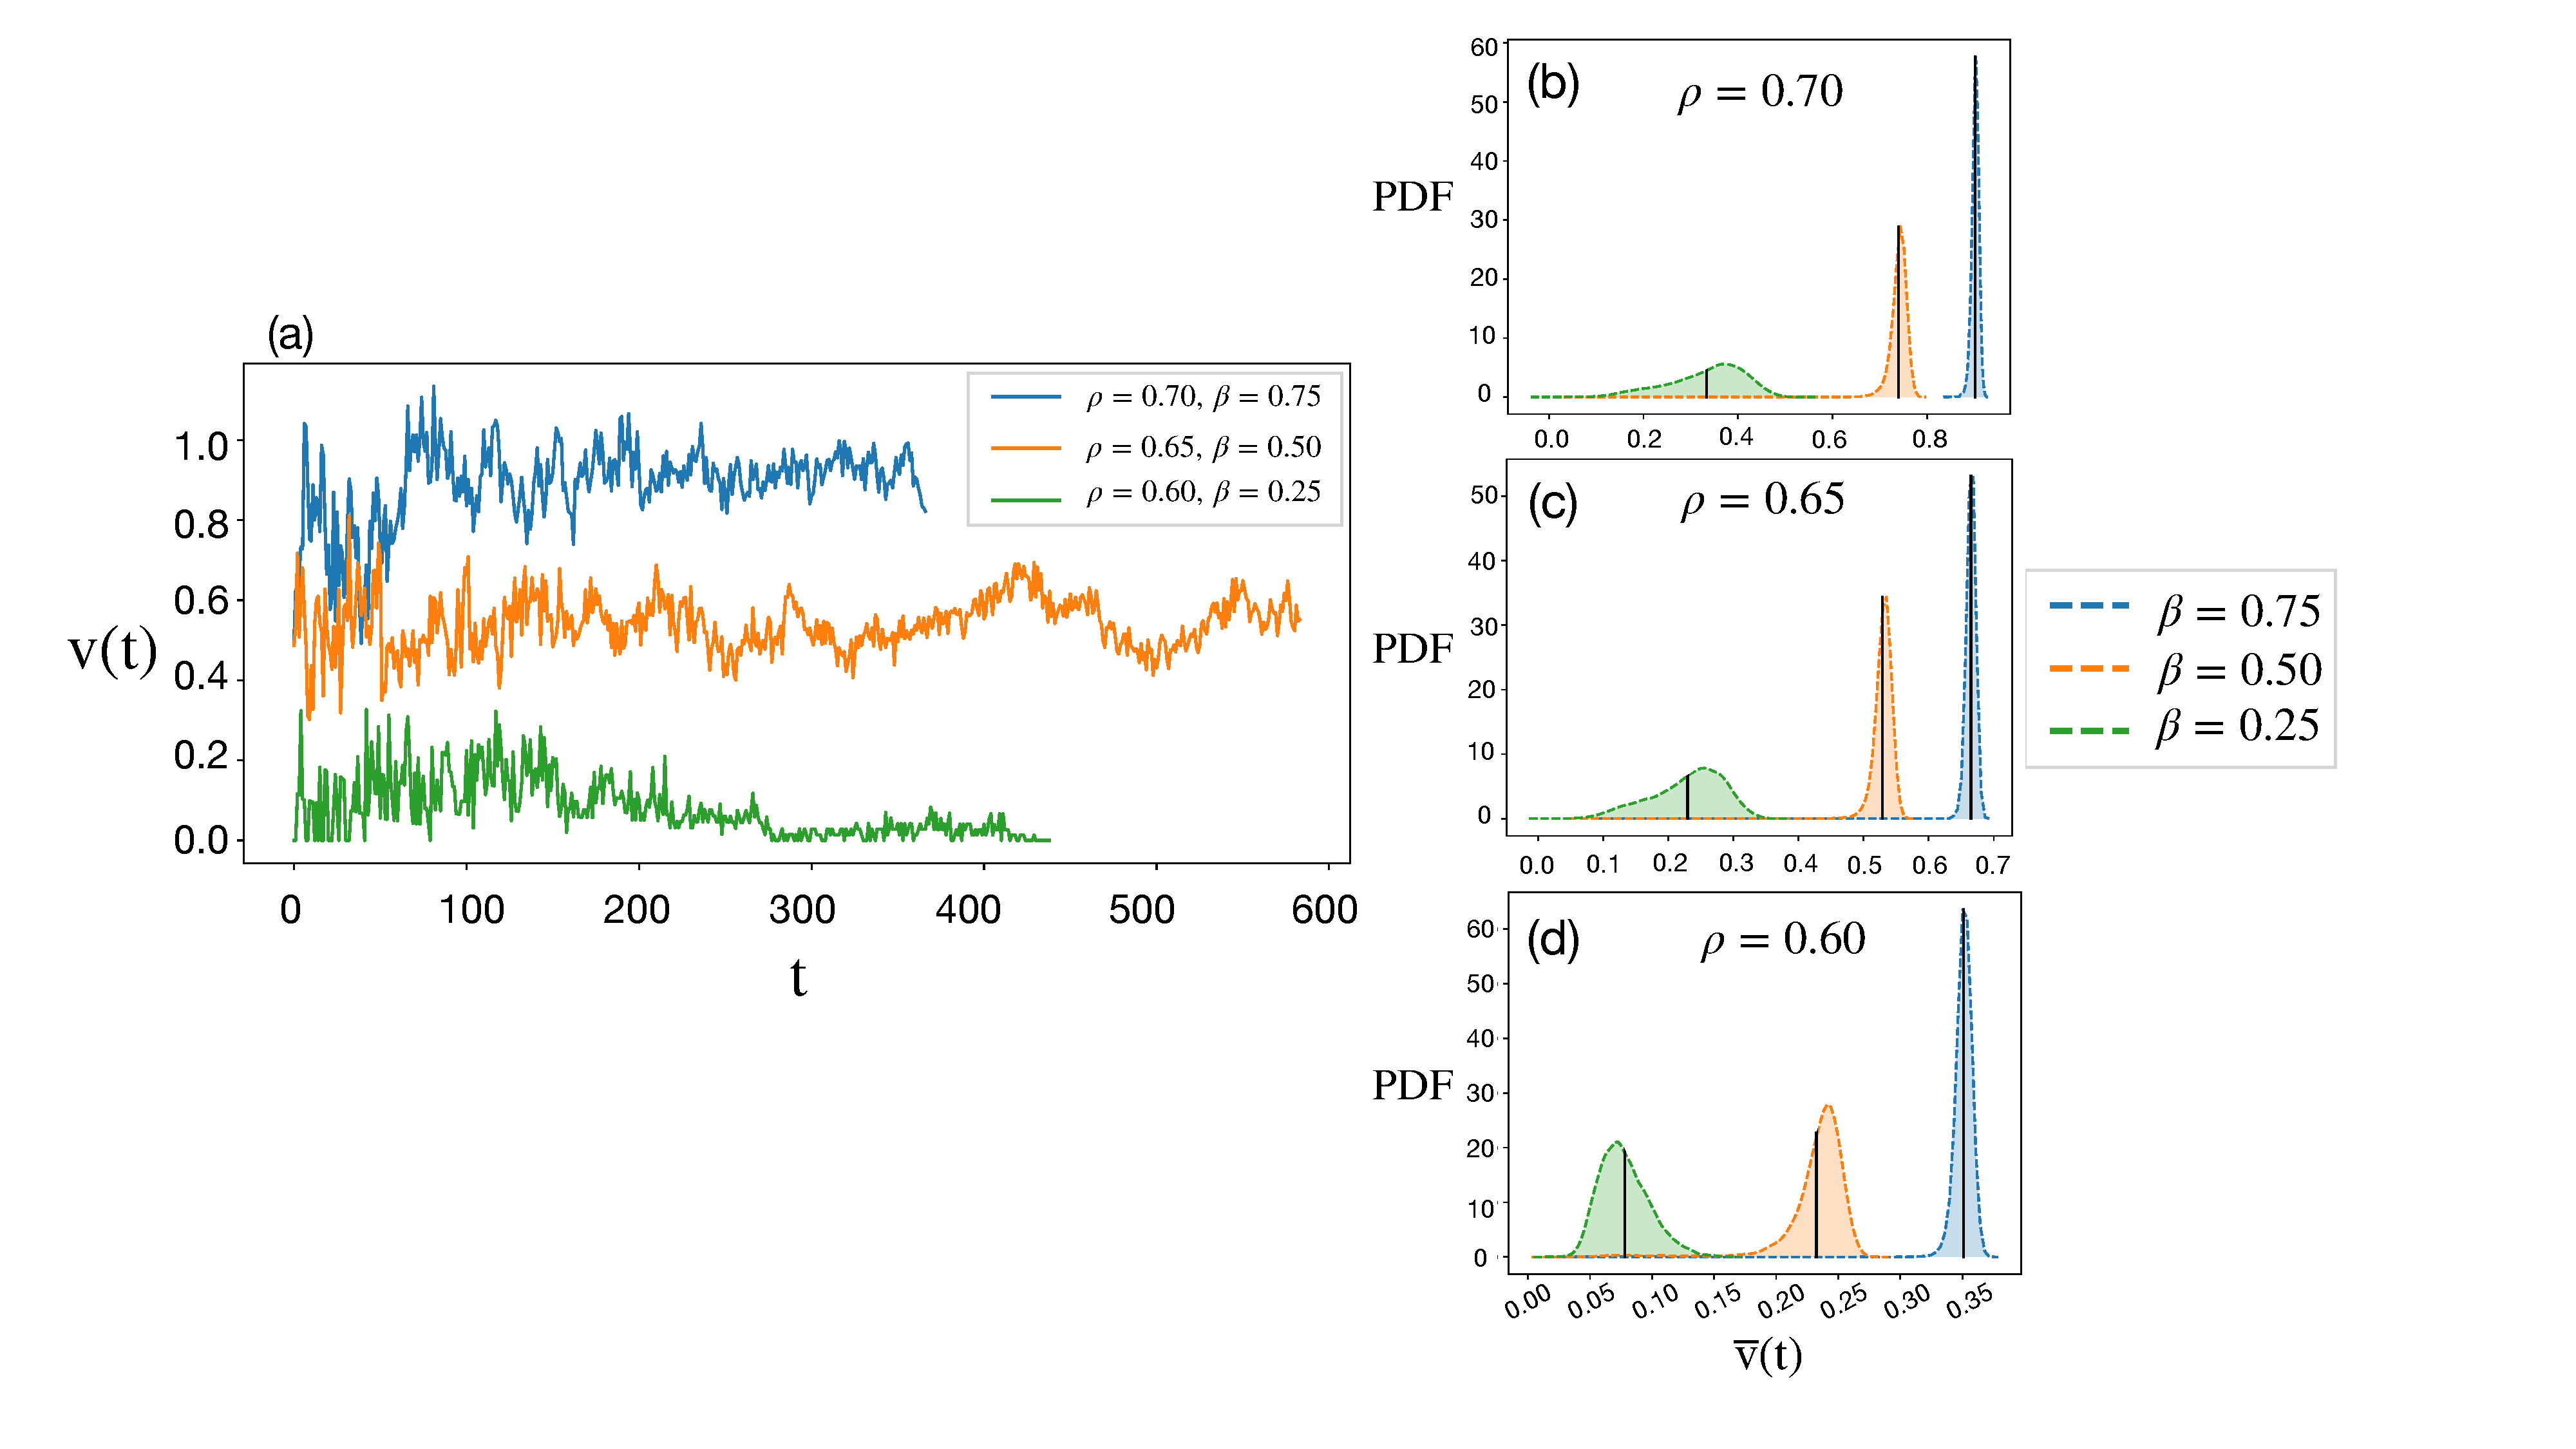
\includegraphics[scale=0.26]{chapter3/figures/figure7.pdf}
    \caption{(a) The velocity metric time-series $v_{radial}(t)$ is shown for three typical simulations, higher values of $\rho$ and $\beta$ give higher mean values of propagation speed. (b-d) The probability density function of mean spreading velocity $\big\langle \overline{v}_{radial}(t) \big\rangle$ for variations in $\rho$ and $\beta$.}
    \label{fig:vel_eff_rad_metric}
\end{figure}

Figure \ref{fig:slm_pspace} contrasts the epidemic threshold according to both percolation and velocity-based metrics.
In Figure \ref{fig:slm_pspace}(a), a one-dimensional line through the parameter-space of $\rho$ reveals the percolation probability for the three different infectivity parameters shown.
The vertical dashed line shows the accepted percolation threshold, $\rho_c$, for a two-dimensional square lattice. 
For $\beta \in [0.50, 0.75]$, the probability of percolation is identical to that shown in Figure \ref{fig:ch3-perc-pr};
However, a lower value of $\beta = 0.25$ decreases the percolation threshold, as evidenced by the green line shifting to the right.
Figure \ref{fig:ch3-perc-pr}(a) intuitively demonstrates that a pathogen with a low value of infectivity requires a more significant tree density to spread.

The ensemble-averaged radial velocity $\big\langle \overline{v} \big\rangle$ (as per Equation \ref{eq:vel_eff_r}) mirrors the percolation threshold,
notwithstanding with some differences.
In Figure \ref{fig:slm_pspace}(b), we witness a significant increase in the propagation speed when the density crosses the threshold density $\rho_c$, 
notably for $\beta=0.75$ and $\beta=0.50$ shown in blue and orange. 
In addition, a higher $\beta$-value predictably yields a higher radial velocity, both before and after the epidemic transition.

Interesting behaviour is discerned by the contrasting the green curves (when $\beta=0.25$) in Figures \ref{fig:slm_pspace}(a-b);
the vertical dashed green line in Figures \ref{fig:slm_pspace}(a-b) highlight when epidemics begin to propagate to the domain edge reliably.
Therefore, when $\beta=0.25$ the velocity remains close to zero, yet the percolation probability is high. 
This observation indicates a regime of persistence in the model, where epidemics can survive for long periods, barely above the threshold \cite{gilligan2008epidemiological}.

The equivalent two-dimensional plots over the full parameter-space of $\rho$ and $\beta$ are shown in Figures \ref{fig:slm_pspace}(c-d) for percolation and radial-velocity respectively. 
The two-dimensional percolation probability depicts an abrupt transition between two stable regimes of extinction and epidemic, where
a narrow range of critical parameters $\rho_c$ and $\beta_c$ separate epidemic and extinction.
In contrast, Figure \ref{fig:slm_pspace}(d) shows the ensemble-averaged velocity that describes a smoother transition between states.
Therefore, one might argue that percolation captures the threshold with greater clarity as the distinction between epidemic states is more apparent.

One significant difference between the percolation and velocity-based metrics is that percolation depends trivially on infectivity beyond $\beta \approx 0.40$;
meanwhile, the radial velocity tends to increases for higher infectivities.
Between $0.15 <\beta<0.30$, a higher value of $\rho$ is needed for percolation to occur;
the equivalent velocity-based behaviour can also be seen, albeit with a more continuous transition.
A higher infectious lifetime $T$ lowers $\beta_c$, as more infectious time-steps increase the chance of secondary infections, thus lowering the threshold.
Here, the parameter-sweeps can be understood to portray an `\textit{epidemic phase diagram}'.

\begin{figure}
    \centering
    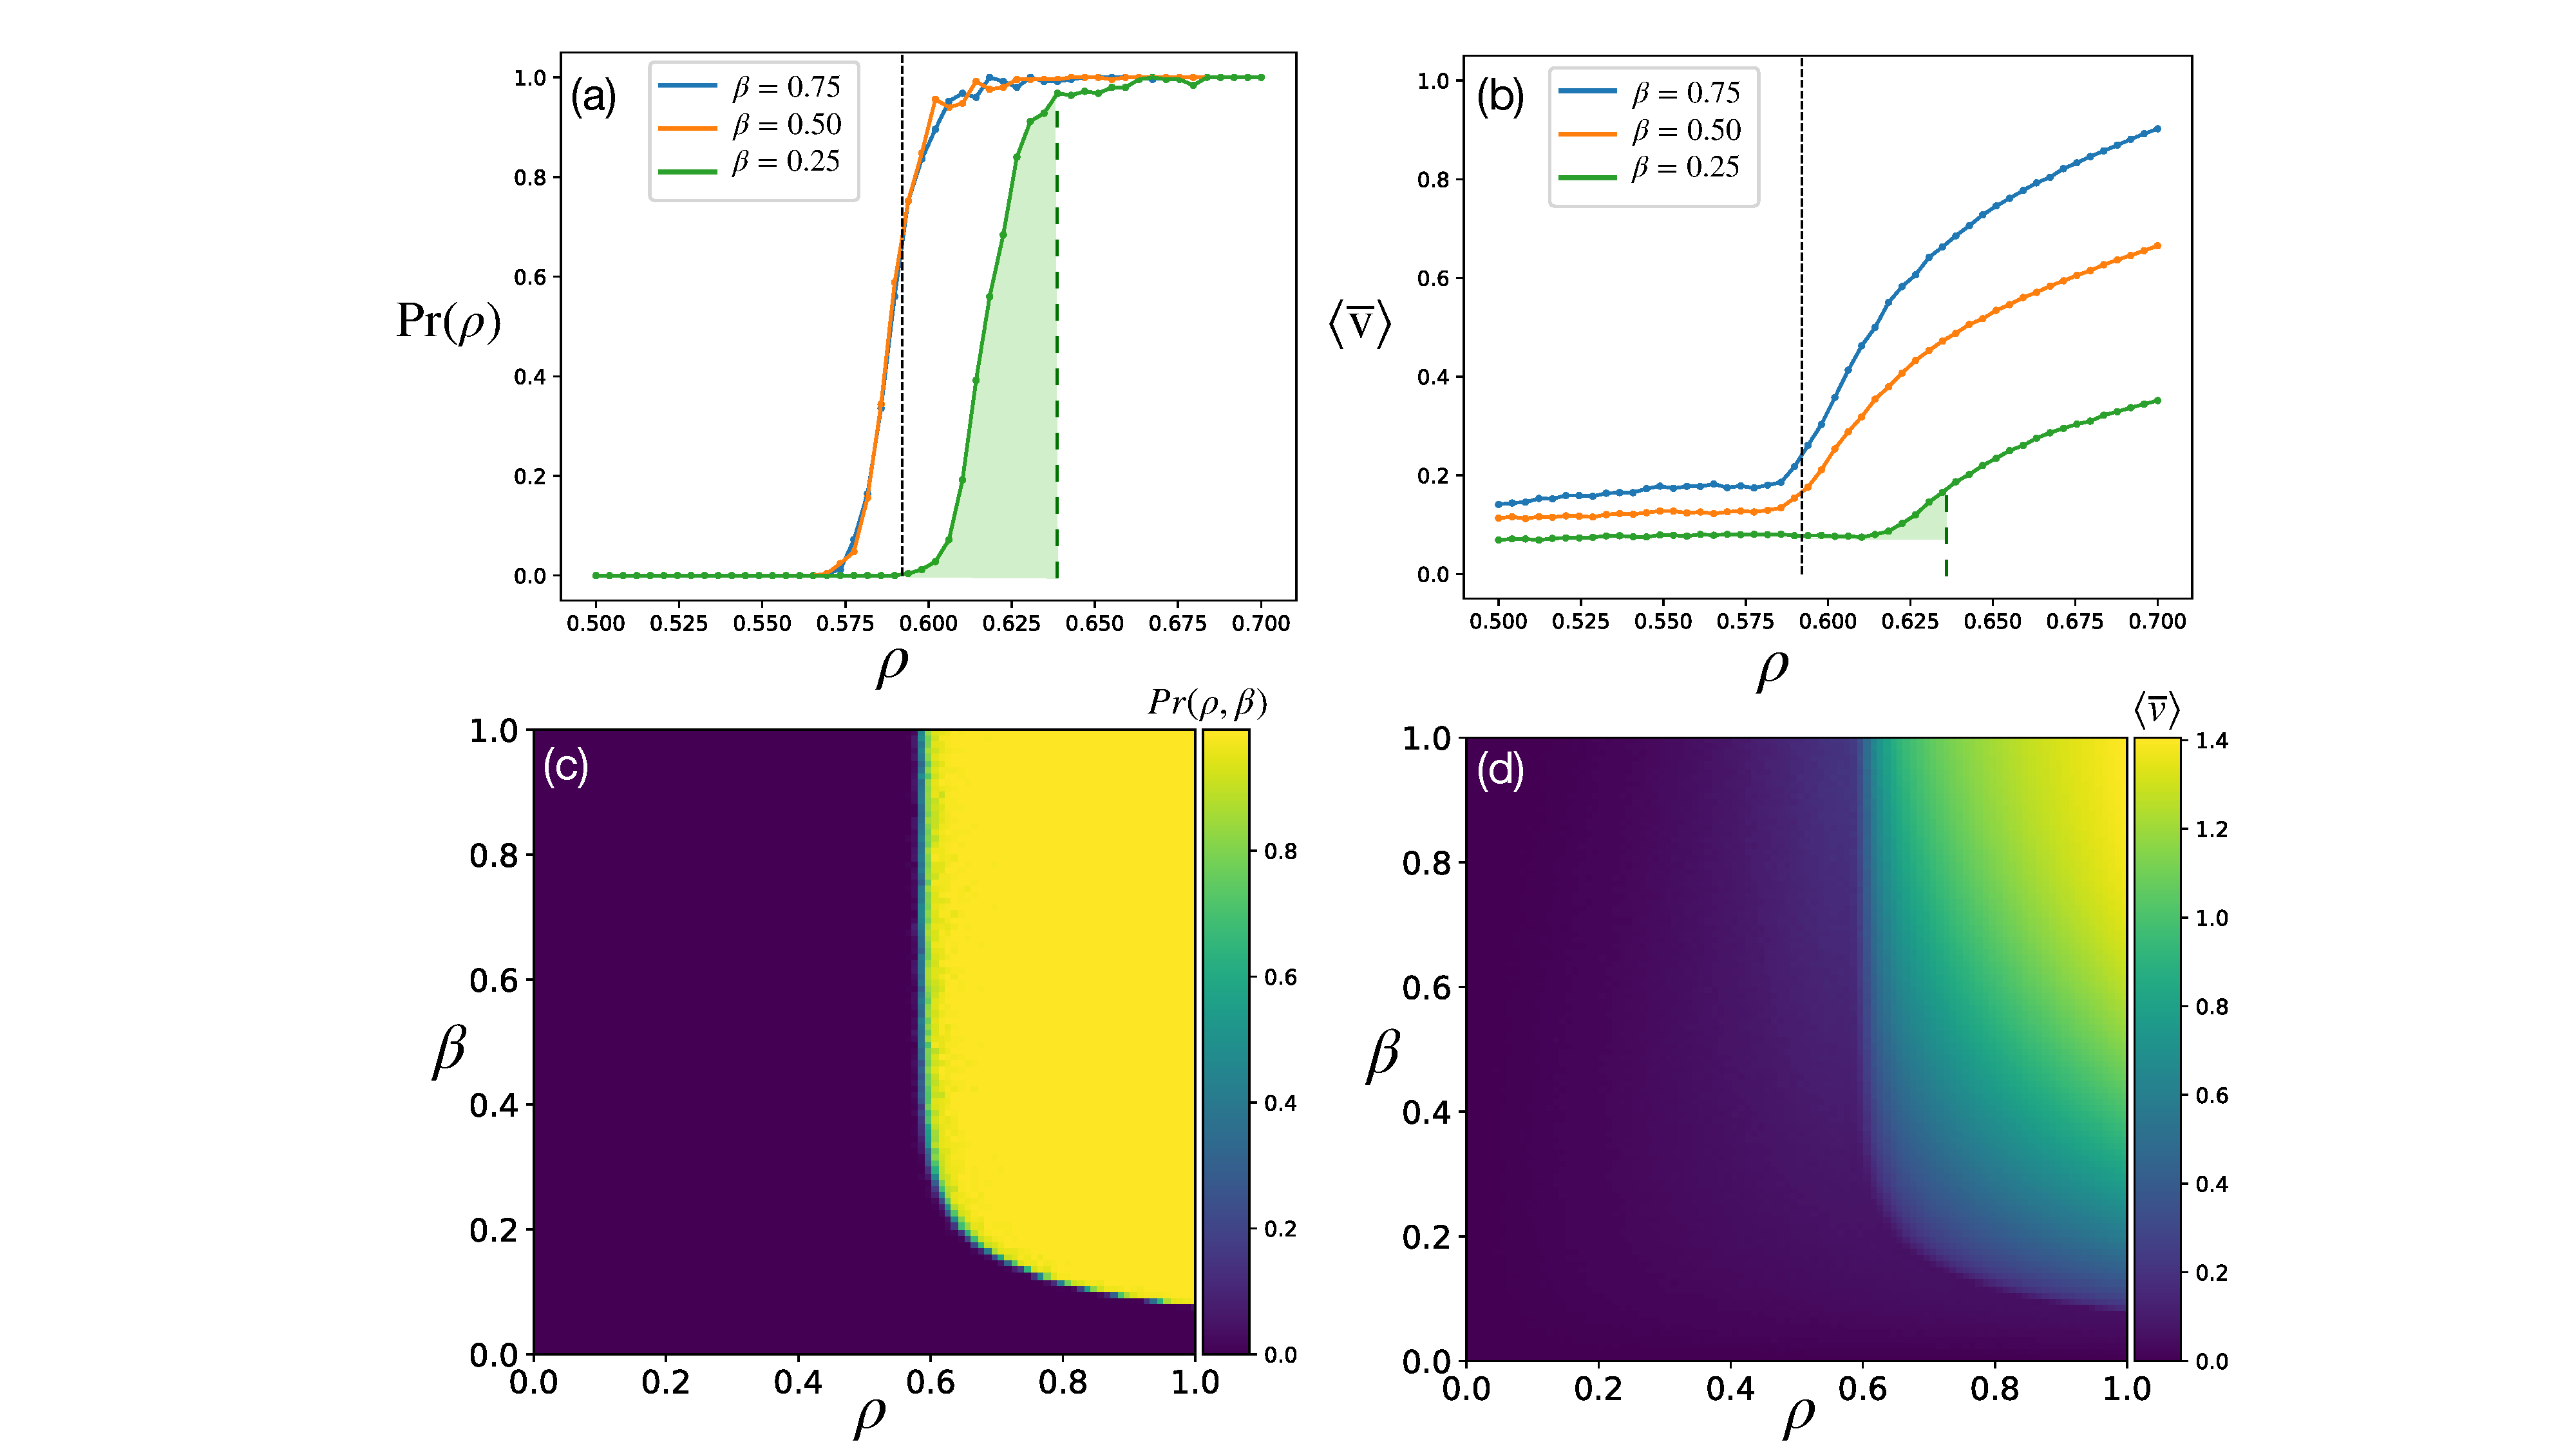
\includegraphics[scale=0.325]{chapter3/figures/figure4-perc-vel-phase-trans.pdf}
    \caption{
    A parameter sweep of $\rho$ and $\beta$ over the $500\times500$ domain. (a-b) The percolation probability is shown alongside the radial velocity over a one-dimensional parameter-space of $\rho$. For the lower-valued infectivity of $\beta=0.25$, the density threshold is slightly higher than classical percolation  $\rho_c=0.592$, indicated by the vertical dashed line. A gradual increase occurs when using the radial velocity, whereas percolation shows an abrupt transition. (c-d) A two-dimensional parameter sweep paints a similar picture.
    }
    \label{fig:slm_pspace}
\end{figure}

\newpage

\section{Chapter Summary}

This chapter introduced percolation theory, leading to a one-parameter percolation $SIR$ model of tree disease spreading through a forest.
The one-parameter model demonstrated stochasticity on account of the randomly populated host distribution inside a square lattice. 
Assessing the model on one lattice configuration signifies a limitation in our analysis; 
more rigorous treatments might consider examining the spread of disease on alternate lattices.
However, although only one lattice was employed, universal properties of the model would be expected to remain the same\textemdash such as the critical exponent describing the correlation length $\xi$\textemdash as discussed in section \ref{section:universality}.

In section \ref{ch3:two-param-model}, an infectivity parameter ($\beta$) was included in the model.
The infectivity parameter introduced temporal stochasticity into the system, as infections spread probabilistically between nearest neighbours \textemdash
as opposed to the one-parameter model that spreads between hosts with a probability of one.
The infectivity parameter altered the critical density; 
higher values of $\beta$ recovered the standard percolation threshold for a two-dimensional square lattice ($\rho_c\approx 0.592$), 
while lower values of $\beta$ increased the critical density required to support an epidemic.

In nature, a pathogen might interact with diverse hosts over various environmental conditions;
a relevant and interesting example includes the algae-like oomycete \textit{Phytophthora ramorum} (\textit{P. ramorum}). 
The pathogen \textit{P. ramorum} affects a wide host range \cite{GRUNWALD2012131}, 
including Larches (deciduous conifers of the genus \textit{Larix}) and southern beech (\textit{Nothofagus}), 
and some non-native oaks such as red oak (\textit{Quercus rubra}) \cite{grunwald2008phytophthora}.
Although, different genetic variants of \textit{P. ramorum} affect different hosts with varying severities.
For example, north American oak speceis are highly suceptible to the NA1 lineage \cite{rizzo2002phytophthora}, 
while UK larch trees appear highly suceptible to the European lineage EU1 \cite{king2015planta}. 
Therefore, the integration of $\beta$ in the SLM is undoubtedly simplistic and general; nevertheless, it permits a description of varying degrees of pathogen virulence.

Two metrics categorized the model's behaviour: the pathogens average radial velocity alongside a probability of percolation.
The percolation probability defined a sharper, more reliable transition between epidemic and pathogen extinction.
Although the percolation probability may prove more beneficial for classifying epidemic regimes, 
the radial velocity captured a similar threshold-like behaviour beside additional dynamic information in the form of a time series.
Subsequently, the time series was ensemble-averaged and examined over a sweep of $\rho$ and $\beta$ values. 

Interestingly, comparing the percolation probability to radial velocity revealed a parameter region above the threshold where the pathogen survives but slowly propagates to the domain boundary. 
This behaviour approximates persistence; the reader can find a review of invasion and persistence in section \ref{ch3:invasions_and_persistence}.
However, neglected host population dynamics in the SLM prevents long-term coexistence between host and pathogen, 
an essential requirement of persistence \cite{gilligan2008epidemiological}. 
Accordingly, the SLM only approximates invasion and persistence, which therefore signifies a limitation in the framework. 

As we look to construct a more representative model, it is worth remarking on the most significant assumptions that underpin the SLM:
\begin{enumerate}
    \item \textbf{Local NN interactions}: in reality, many dispersal mechanisms exist to propagate the spread of disease\textemdash 
    section \ref{ch2:dispersal} contains more information. 
    Undesirably, local interactions in the SLM revealed unnatural artefacts of lattice geometry.
    Moreover, as the pathogen could not jump over empty lattice sites, epidemics were only possible above the percolation threshold, 
    i.e. when connected clusters of hosts span the domain.  
    
    \item \textbf{Uniform dynamics:} in general, pathogen-host interactions transpire with varying degrees of severity; 
    for example, age-dependent severity in ash dieback and the species-level virulence of 
    \textit{P. ramorum}. 
    In contrast, the SLM considers that A) the transition probability into $R$ occurs with a uniform number of steps 
    B) the probability of transition into $I$ is identical between hosts 
    C) $\beta$ is simplistic, with no spatio-temporal (environmental) dependence. 
    More generally, we have constructed a general, abstract model with no specific pathogen in mind.
    
    \item \textbf{Host distribution}: natural tree populations present rich spatial structures with varying degrees of clustering and aggregation \cite{doi:10.1086/342823}.
    Indeed population clustering has been confirmed over various spatial, from the tree-level to the field-level \cite{wiegand2007analyzing}.
    Therefore, the flat randomly distributed host population considered in this chapter falls short of a realistic description.
    Moreover, the SLM describes the spread of disease in a densely populated forest, and as we look to model the spread of disease over Great Britain realistic tree canopy cover data should be incorporated into the framework.
\end{enumerate}
Despite the assumptions and simplicity of the SLM, it provides a general setting upon which to elaborate.
The next chapter outlines all the applications that were investigated using the SLM.
\newpage 

% % % % 4) Application of the simple lattice model--moving to a realistic host landscape
% -----------------------------------------------------------------------------
% 1) Move to a map of the UK 
% 2) show edge effect and epicenter changes
% 3) introduce the data-set in a formal capacity + define the threshold function
% 4) show how heterogeneity changes the problem i.e. discontinuities in the phase diagram
% -----------------------------------------------------------------------------

\chapter{Simple lattice model: applications}
\label{chapter:SLM-applications}

Previously, a percolation-based $SIR$ model of tree disease spreading through a forest was outlined, named the simple lattice model (SLM).
The SLM provides a flexible foundation for generalising as we look to model the spread of disease over realistic landscapes focused in Great Britain.
This chapter aims to examine some applications of the SLM.
In particular, two applications divide the chapter, beginning with the early warning systems (EWS) for forest management and ending with a toy model of landscape-level spread.

Firstly, the system for EWS detection put forward by \cite{OROZCOFUENTES201912} is extended; the original publication considered one fixed parameter of $\beta$, here we generalise the analysis to the entire $\beta$ parameter space. In addition, we employ an alternative metric that permits a more precise EWS detection.
Secondly, the SLM will be adapted to construct a toy model of landscape-level epidemics in Great Britain.
More specifically, units of individual trees in the SLM are re-scaled to $\mathrm{1km \times 1km}$ patches 
and projected onto a predicted oak abundance data set given by \cite{hill.data}.
The toy model denotes the first step towards a more representative framework over realistic landscapes.

\section{Early warning signals}
\label{sec:EWS}

Applications of early warning signals have been investigated by \cite{OROZCOFUENTES201912} for forest management and ecosystems services.
The results focused on a one-dimensional parameter space of tree density $\rho$ over a square lattice with fixed infectivity $\beta$.
The study observed statistically significant changes (or signals) in the
moment-generating functions (of variance, skew and auto-correlation) for the radial velocity.
Changes in variance, skew or auto-correlation can preempt epidemic phase transitions, 
thus providing helpful information that could aid forest and plantation managers to maintain tree health. 
Here, we offer a small extension to some of the concepts presented by \cite{OROZCOFUENTES201912}.
In particular, a new domain and metric are used to detect more precise, early warning signals.  
The analysis is generalised to two dimensions in the parameter-space of $\rho$ and $\beta$. 
After introducing these alternative concepts, we discuss some of the problems and complexities encountered with ensemble-averaging. 

\subsection{Cylindrical geometry}

The metric used by \cite{OROZCOFUENTES201912} to quantify early warning signals had a similar form as Equation \ref{eq:vel_eff_r}, albeit with the inclusion of $N_R$.
That is, the results included both the infected and removed ($N_{I+R}$), whereas Equation \ref{eq:vel_eff_r} is based on just the infected ($N_I$). 
Unfortunately, the radial velocity (based on the number of infected and removed trees) can lead to confusing results, as geometrical effects alter the a rate of increase as the wave spreads outward; this is particularly visible for later times when the wavefront extent is considerable.\footnote{See Figure 4d in \cite{OROZCOFUENTES201912}, the apparent rate of increase in the velocity metric is purely due to geometry artefacts and the metric definition.}.
We will use an alternate lattice geometry to mitigate geometric effects.

Consider a rectangular domain of size $[L_x, L_y]$ where $L_x>L_y$ and $(x, y)$ represent dimensions of width and height respectively.
Figures \ref{fig:ews-primer}(a-c) shows the domain, henceforth referred to as the `channel' domain, over three time-steps for parameters above the threshold, $\rho=0.65$ and $\beta=0.50$.
The initial conditions are adjusted, so the first column (denoted by $x_0$, taken as the origin) is infected.
In addition, the boundary conditions permit the disease to propagate freely in the $+x$ and $\pm y$ directions, thus realising a cylindrical geometry with periodic boundary conditions in $y$ direction and fixed boundary conditions in $x$.

We register a percolation event in the channel domain if an infected tree reaches the last column, denoted by $x_m$
The percolation threshold shifts toward higher densities if the domain is sufficiently narrow (having a high aspect ratio), as the dimensionality of the travelling wave to somewhere between one and two dimensions\footnote{Additionally less space in computer memory is occupied and simulation time is lowered}. 
The higher percolation threshold can be explained by gradually increasing the domains aspect ratio;
in the limit $L_y = 1$ and $L_x  \gg 1$, a one-dimensional domain is realised, and the critical host density increases to $\rho_c=1$, i.e. the well-known one-dimensional percolation threshold.

As expected, studies have confirmed that site and bond percolation in two and three dimensions depend critically on a cylinders aspect ratio \cite{sangare2009continuum}.
Therefore, we choose an aspect ratio that approaches the percolation threshold for a two-dimensional square to keep consistent with the numerical results of chapter \ref{chapter:SLM}. 
In practice, a channel of size $(L_x, L_y) = (350, 50)$, was sufficient, as shown through Figures \ref{fig:ews-primer}(a-c). 

\newpage

\begin{figure}
    \centering
    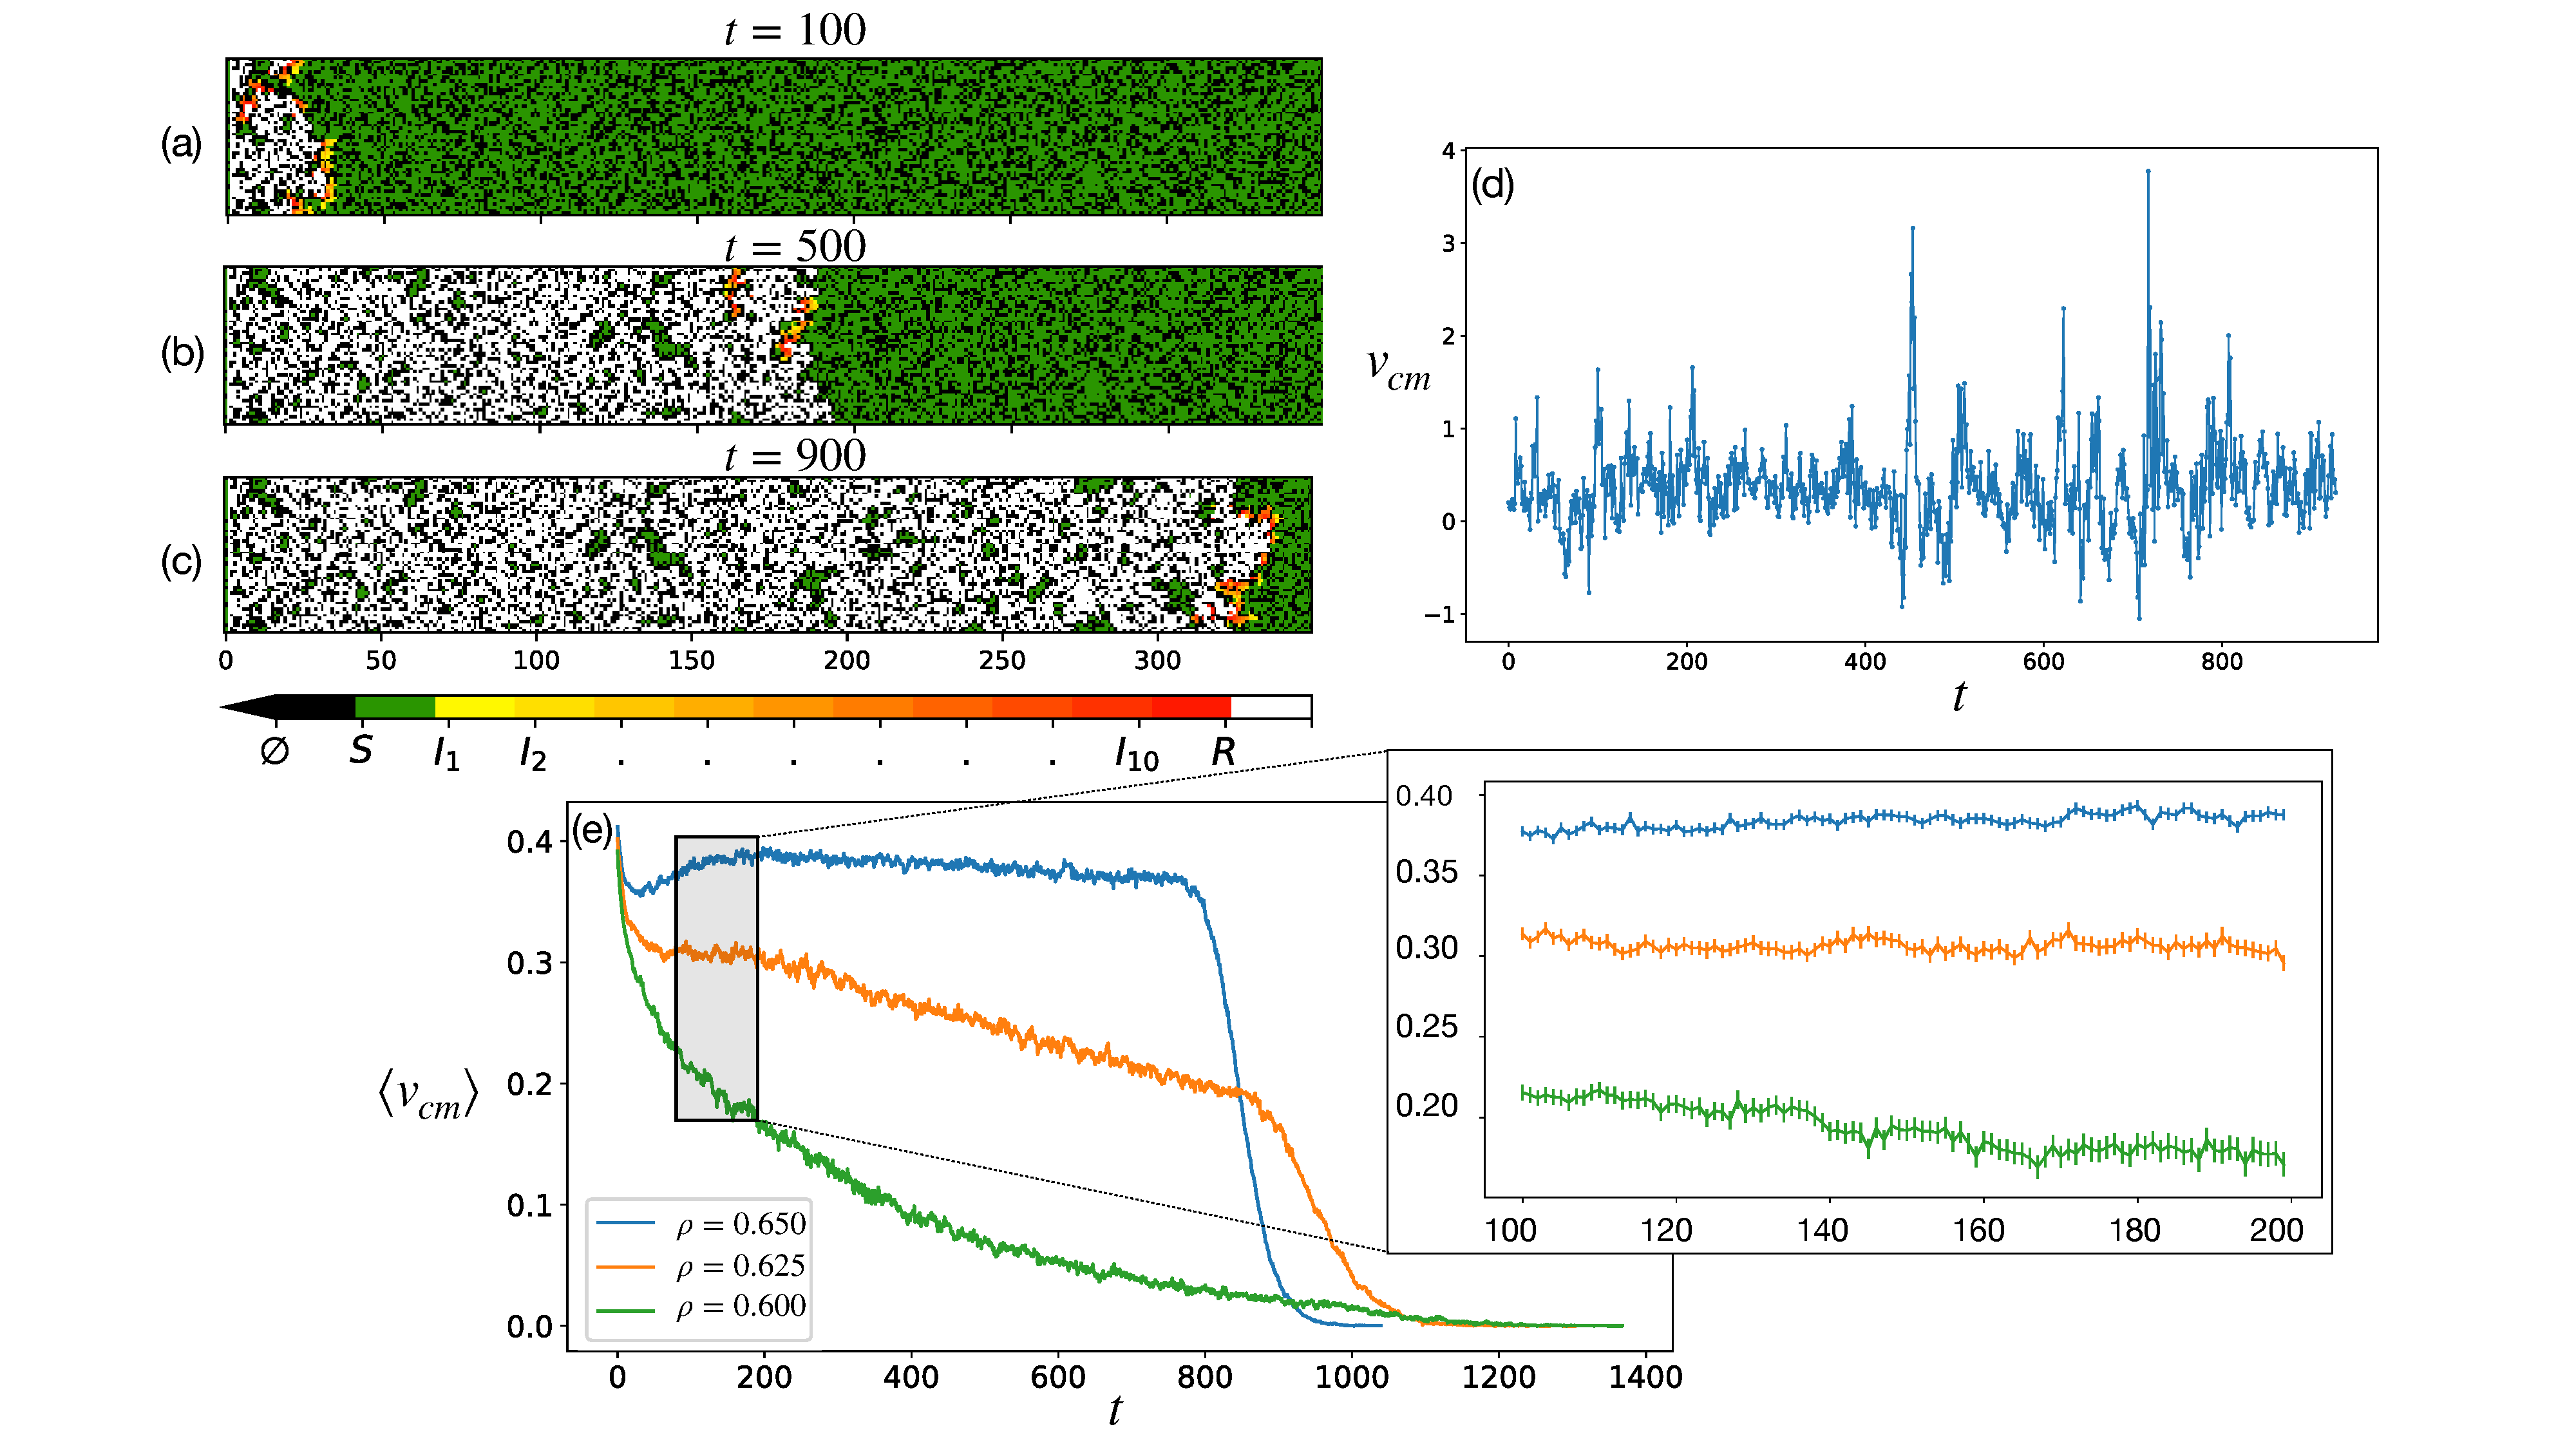
\includegraphics[scale=0.30]{chapter4/figures/figure1-channel-domain.pdf}
    \caption{
    (a-c) A channel domain of size $50\times350$ is shown over three time-steps for model parameters $\rho=0.65$ and $\beta=0.50$. 
    The center of infectious mass is recorded for each time-step. 
    (d) Plots of the center of mass time-series for the simulation illustrated in panels (a-c). 
    (e) The mean center of mass time-series (of $10^4$ repeats) for three variations in density and $\beta=0.50$. 
    Time-series begin to decay around the mean simulation run-time.  
    The zoomed inset shows the ensemble averaged time-series for $t\in[100, 200]$ and reveals increases in error bars lower density parameters.
    }
    \label{fig:ews-primer}
\end{figure}

\subsection{Centre of infectious mass}

The channel domain provides an advantageous setting to capture early warning signals, avoiding two-dimensional geometrical effects.
Moreover, the channel permits an improved (more intuitive) `centre of mass' metric (COM), based on the mean infectious tree displacement from the origin:
\begin{equation}
   v_{cm}(t) = \frac{\sum^i x_i(t)}{N_I(t)} - \frac{\sum^i x_i(t-1)}{N_I(t-1)}
   \label{eq:COM}
\end{equation}
where $x_i(t)$ is the spatial location along the $x$ axis of the $ith$ infected tree at 
time $t$ and $N_I(t)$ is the total number of infected trees at time-step $t$. 
 The form of Equation \ref{eq:COM} displays intrinsic similarities to the Newtonian center of mass:
 \[x_{cm} = \frac{\sum^i x_i\times m_i}{\sum_i m_i}\]
(where $m_i=1$ and $\sum^im_i= N_I$ in Equation \ref{eq:COM}).
Subsequently, the COM velocity will denote the metric defined by Equation \ref{eq:COM}. 
Figure \ref{fig:ews-primer}(b) depicts the COM time-series corresponding to the simulation shown in Figure \ref{fig:ews-primer}(a). 
The COM time-series allows for negative values and looks different to those shown previously in Figure \ref{fig:vel_eff_rad_metric}(a).

Figure \ref{fig:ews-primer}(c) illustrates the COM ensemble-average, denoted by $\langle v_{cm}\rangle$, for the three values of tree density.
On average, the mean time series begins to decay after the mean lifetime of the simulation; the blue time-series shows a drastic decrease around $t \in [800, 900]$, which coincides with the pathogen reaching the domain boundary\textemdash also reflected in Figure \ref{fig:ews-primer}(c).
The green time series lies just above the threshold for percolation, and it decays more gradually $t=0$ because of the higher pathogen extinction probability. 
A small number of long-lasting simulations with run times (exceeding $t>1000$ steps) occurred in the green time-series, indicating criticality in the system\textemdash 
previously likened to a regime of persistence in section \ref{sec:SLM-epidemic-threshold}.
The inset of Figure \ref{fig:ews-primer}(c) shows the ensemble-averages between $t\in [100, 200]$, plotted beside the standard error for each time-step.
Error bars are most significant for the lowest-valued density shown in green, capturing a more chaotic spread.
In principle, if the variance signature looks different before and after the epidemic regime, an early warning signal can be detected. 

\subsection{Ensemble averaging method}

The findings of \cite{OROZCOFUENTES201912} were gathered by first producing a distribution of mean time-series velocities $\overline{v}_t$.
In this scheme, an early warning signal is detected from the statistical moment-generation functions over the mean velocity: e.g. $var\big\langle \overline{v}_t \big\rangle$,
analogous to calculating variance, skewness and autocorrelation over the distributions of Figures \ref{fig:vel_eff_rad_metric}(b-d).
However, calculations based on the mean simulation variance, $ \big\langle \overline{var}({v}_t) \big\rangle $ were found to reveal a clearer EWS.
Consequently, we proceed by detailing an ensemble method that permits the capture of within-simulation variance. 

Before the ensemble averaging method is elaborated, it makes sense to define the relevant notation.
Suppose a simulation with parameters $\rho, \beta$ propagates for $f$ time-steps, Equation \ref{eq:COM} describes the time series as: $v_{cm}^{t=1}, v_{cm}^{t=2},..., v_{cm}^{t=f} \in V^{\rho\beta}$. 
Then, a set of independent time series are generated by repeating $N$ simulations. 
A set of $N$ repeated simulations for an arbritrary point in the parameter-space ($\rho, \beta$) 
can be labelled as: \{$V_1^{\rho\beta}, V_2^{\rho \beta},..., V_N^{\rho\beta}\} \in \mathcal{V}_{\rho\beta}$, 
where each $V_i^{\rho\beta}$ describes an individual simulation time series and $\mathcal{V}_{\rho\beta}$ describes the entire ensemble for parameters $(\rho, \beta)$. 
Thus, an early warning signal (EWS) is detected by calculating the mean time-series variance,
defined by:
\begin{equation}
\label{eq:ews_eq}
    \big\langle \overline{var}(v^{\rho\beta}_{cm}) \big\rangle = \frac{1}{N}\sum\limits_{i=1}^{N} var(V_i^{\rho\beta})
\end{equation}

We require the same number of observations within each ensemble to properly analyse the mean time-series variances.
Otherwise, the classification of an early warning signal might be confused with statistical fluctuations and errors.
There are two observations to consider: 
(A) the number of time steps within simulations, i.e. $v_{cm}^{t}$ 
(B) the number of repeated simulations, $N$.
In general, stochasticity will prevent two simulations from having the same number of time steps, 
$|V_i^{\rho\beta}| \neq |V_j^{\rho\beta}|$.
Therefore, short-lived simulations with a small number of time steps might be more error-prone than long-lived simulations;
we introduce a fixed window of time-steps ($t_O\leq t \leq t_F$) to remedy this.
Provided the window length $t_F-t_O$ captures a sufficient number of time-steps, we avoid significant fluctuations in $V_i^{\rho\beta}$. 
Variance inside this window is defined by:

\begin{equation}
\label{eq:ews_eq1}
    \big\langle \overline{var}(v^{\rho\beta}_{cm}) \big\rangle = \frac{1}{N}\sum\limits_{i=1}^{N} var(V_i^{\rho\beta}\Big|^{t_F}_{t_O})
\end{equation}

Initial transience constrains the particular choice of $t_O$ in the channel domain, 
which indeed distorts calculations of the time-series variance\textemdash 
presenting an analogy to the discussion that followed from Figure \ref{fig:vel_eff_rad_metric}(a). 
We set $t_0=100$, as initial instability occurred most over the first $100$ time-steps 
(as shown in Figure \ref{fig:ews-primer}(e), particularly by the blue time series). 
The window upper-bound is to $t_F = 200$ (a two-fold increase of $t_O$) so that simulation variance is measured over a sufficient number of steps.
The variance window of $t_O=100,\ t_F=200$ is justified by noting that an early warning signal is only detectable immediately before 
and after the epidemic threshold; other parameter space regions are less important.
Thus, if the relevant regions in parameter space survive long enough to measure variance in the window $t \in [t_O, t_F]$, 
we may confidently detect an early warning signal.

\subsection{EWS parameter-sweeps}
\label{section:ews_slm}

Figure \ref{fig:ews-results} displays the mean time-series variance, as per Equation \ref{eq:ews_eq1}.
The colour bar shows variance over the entire parameter space of density and infectivity from white to back.
In Figure \ref{fig:ews-results}, the lower and upper red lines indicate a percolation probability of $Pr(\rho, \beta)=0.05$ and $Pr(\rho, \beta)=0.95$, respectively.
Inside these regions, the system transitions into an epidemic and we witness a considerable rise in the variance.

The observations of Figure \ref{fig:ews-results} agree with the results of \cite{OROZCOFUENTES201912}. 
Although measuring EWS over a two-dimensional parameter space reveals some additional information not captured in the original analysis, i.e. when infectivity is low ($\beta<0.40$), EWS preempt the epidemic by a more significant margin\textemdash indicated by the red arrows.
In addition, variance over the epidemic transition appears sharper when $\beta$ is high, as indicated by the darker shade in the upper right quadrant of Figure \ref{fig:ews-results}.

 \begin{figure}
    \centering
    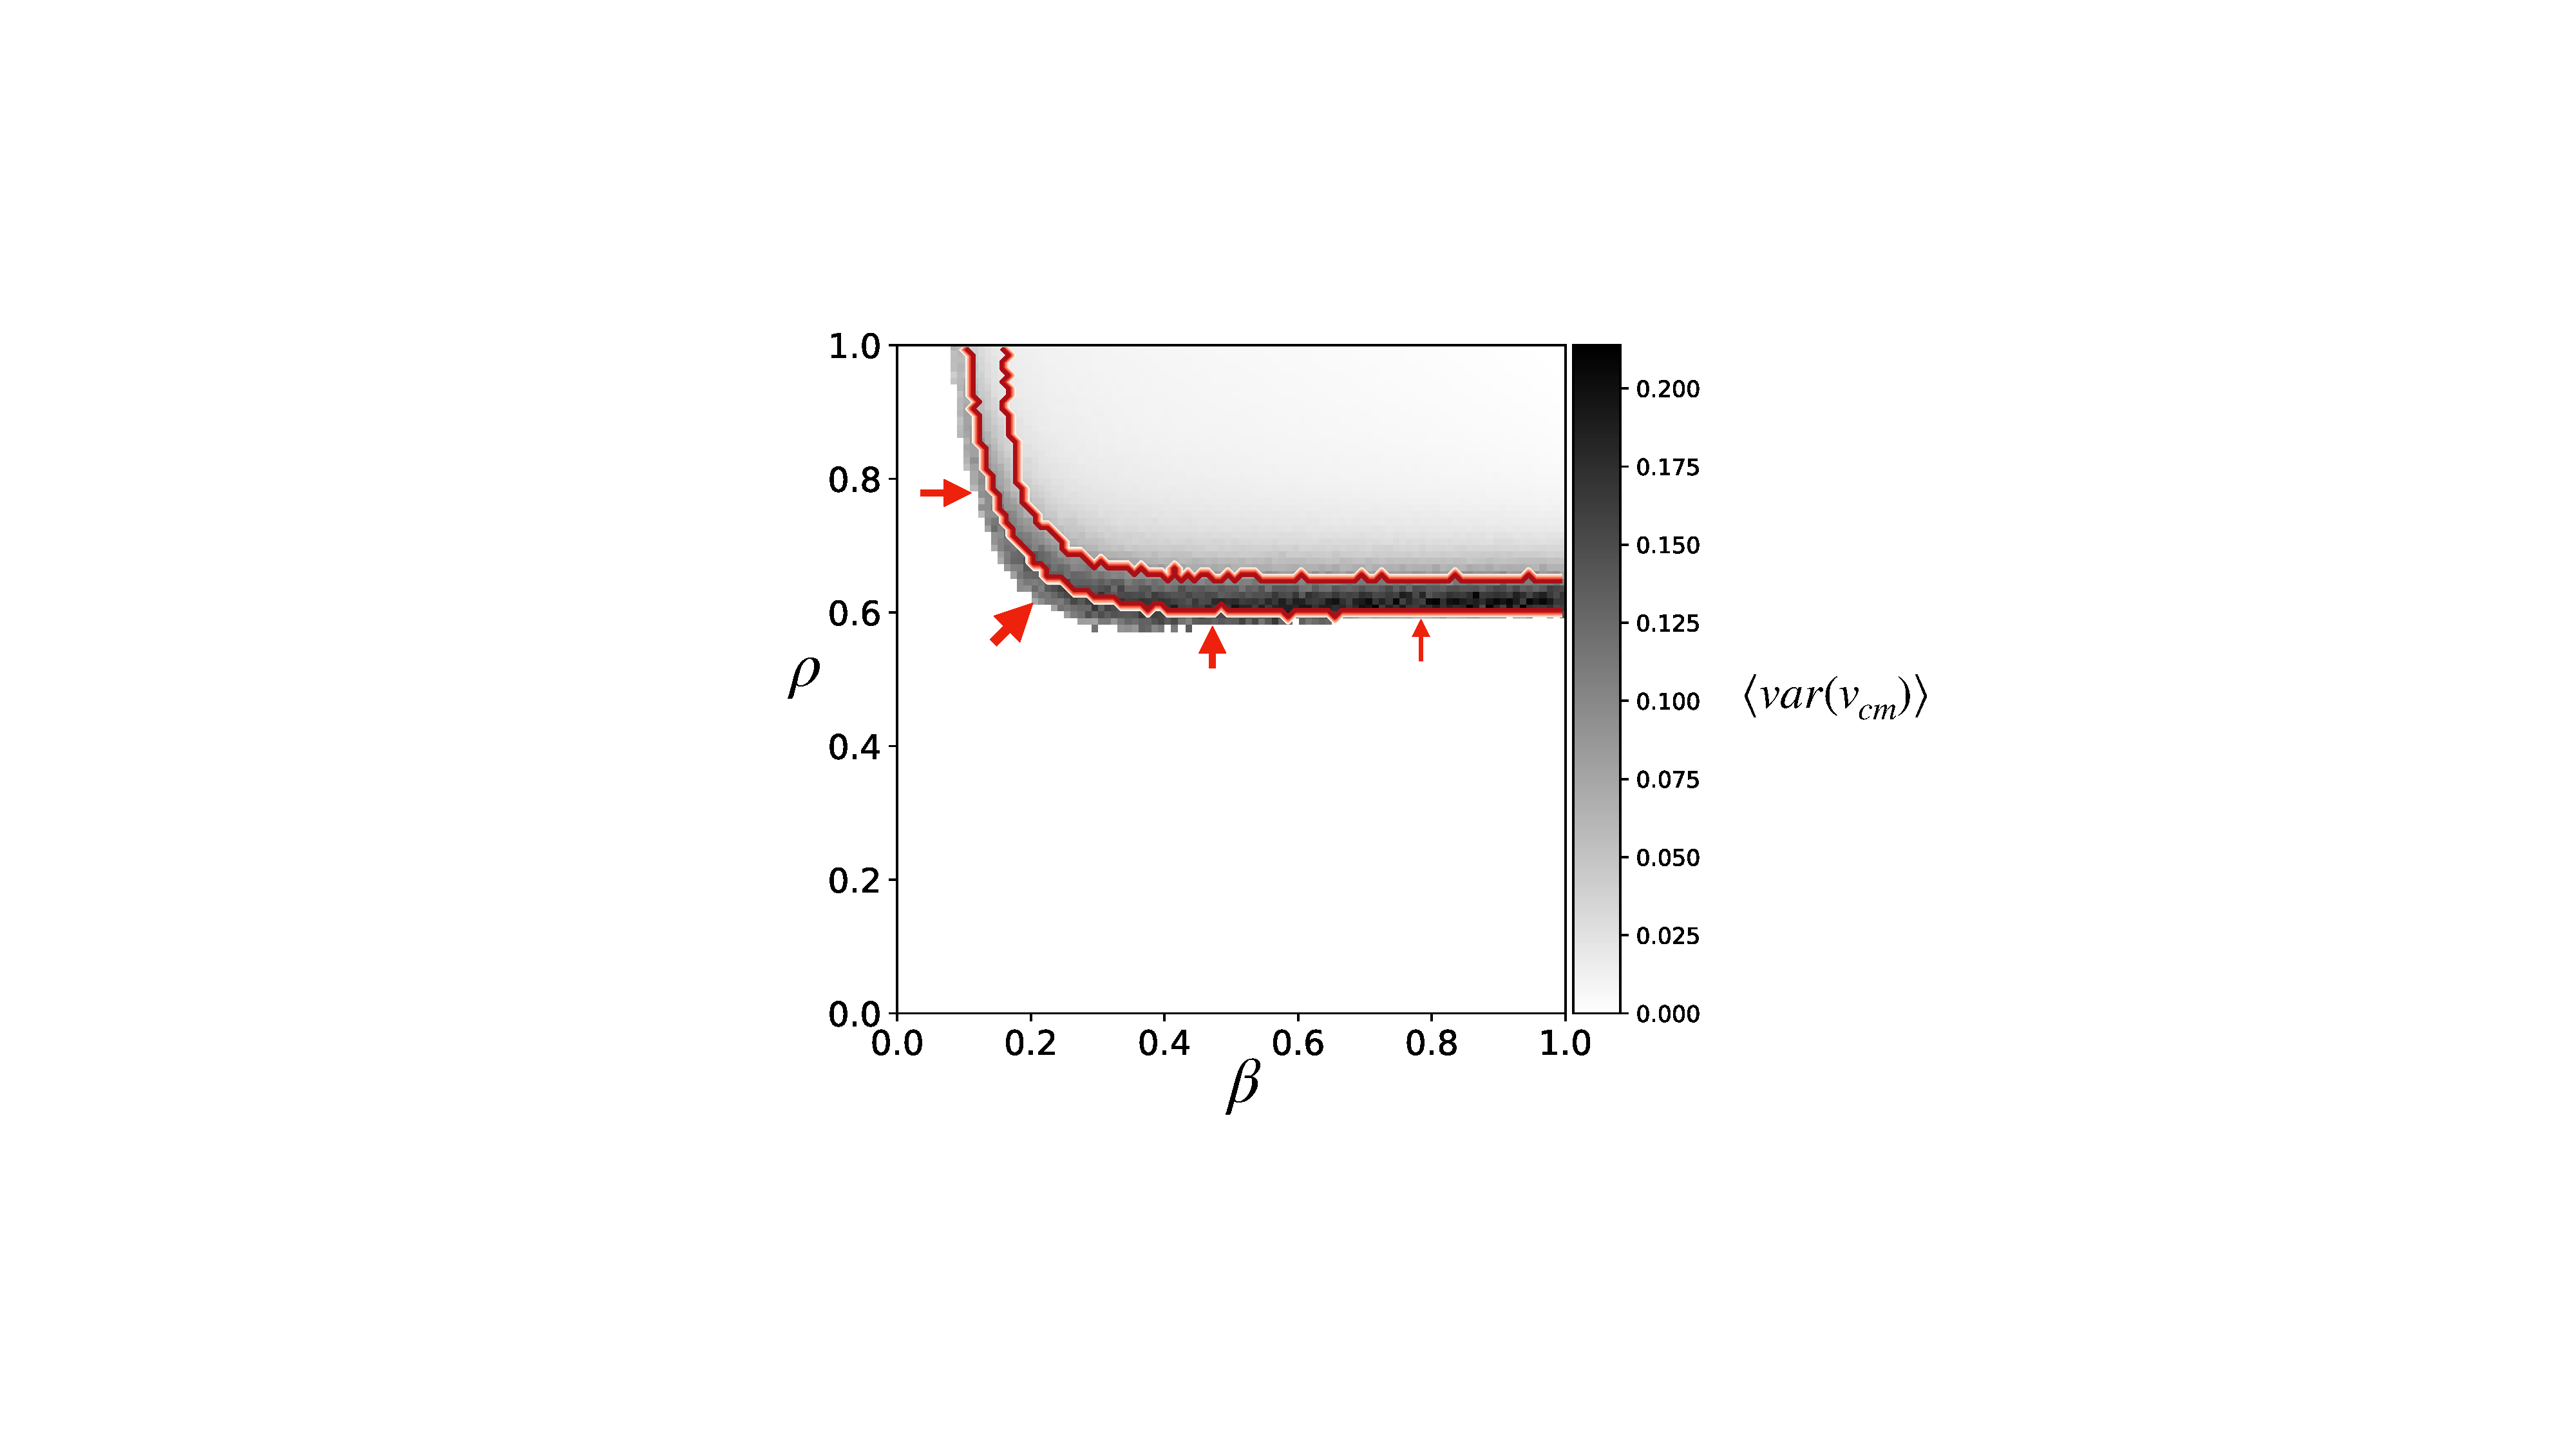
\includegraphics[scale=0.45]{chapter3/figures/figure11.pdf}
    \caption{The ensemble-averaged variance of $v_{cm}(t)$ over a two dimensional parameter sweep of $\rho$ and $\beta$. Red contours show the lower and upper bound of percolation (i.e. between $5\%$ and $95\%$ probability). 
     The epidemic regime is pre-empted by increases in variance more clearly for certain parameter values, %
     indicated by the arrows.}
    \label{fig:ews-results} 
\end{figure}

The following thought experiment can explain the EWS asymmetries in Figure \ref{fig:ews-results}: %
suppose infectivity is high, and density lies just below criticality ($\rho\lesssim\rho_c$), 
so susceptible clusters do not percolate. 
In this case, disease transmission is high on account of $\beta$, 
and all susceptible hosts become quickly infected, 
although an outbreak will come to a halt due to insufficient hosts. Therefore, in this model, 
an aggressive pathogen spreading through low tree densities may propagate rapidly but have a short, 
chaotic signature. Hence the transition is steep,
and the simulation variance is significant, as indicated by the smallest arrow in Figure \ref{fig:ews-results}. 
In this region, detecting an EWS is hard because transitions occur most rapidly.

Now we consider the converse, a less infectious pathogen with an abundance of susceptible hosts, 
located in the top-left region of Figure \ref{fig:ews-results}.
Here, transitions into the $I$ compartment are slower because the pathogen is less infectious, 
although this time, hosts are abundant.
Thus, a pathogen is likely to spread predictably for longer times, 
giving rise to a slightly less abrupt variance signature, 
as indicated by a lighter colour before the transition in the top left quadrant of Figure \ref{fig:ews-primer}.
Although the variance spike is not as significant, 
it preempts the epidemic transition by a more considerable degree\textemdash
indicated by the larger arrows in Figure \ref{fig:ews-results}.
Altogether, Figure \ref{fig:ews-results} suggests that the strength of an EWS depends on the particular combination of epidemic parameters; 
although fundamentally, an EWS is detectable for all parameter combinations
\newpage

\section{A toy landscape-level SLM}

So far, this work has focused on a homogeneous distribution of hosts randomly populating an ideal domain. 
In this section, a toy landscape-level SLM is constructed and simulated on the map of Great Britain.
Modelling the spread of disease over GB entails a large change of scale within the SLM.
Specifically, host units now comprise $\mathrm{1km \times 1km}$ `patches' of land. 
As reviewed in section \ref{ch2:hostdata}, 
collecting high-quality abundance data over large areas is challenging and expensive; 
as such, the SLM is combined with the modelled oak (\textit{Quercus robur}) canopy cover dataset produced by \cite{hill.data}.

\subsection{Realistic boundaries}

Realistic host distributions describe complicated, irregular and heterogeneous domains
known to influence the spread of disease \cite{madden1995plant}.
In contrast, the SLM spreads through a square lattice with regular domain boundaries and homogeneously distributed hosts.
Moreover, the initial conditions (ICs) have been limited to a small number of infected hosts
located at a single epicentre at the centre of a square domain.
However, an epidemic propagating from the centre of a square lattice might look very different
from an epidemic emerging from an arbitrarily located epicentre inside a domain with complicated irregular boundaries.
As a consequence, we examine the interplay of initial and boundary conditions in the SLM\textemdash
compelled further by articles highlighting the importance of domain shape \cite{mikaberidze2016invasiveness},
and critical domain size \cite{abad2020reaction, reimer2017critical}.

As a first step toward modelling with realistic host distribution,
SLM domain edge effects were examined inside the shape of Great Britain.
Figure \ref{fig:uk-spread-primer}(a) shows an outline of Great Britain (GB) filled 
with a random homogeneous distribution of land `patches' at resolution $1\mathrm{km^2}$. 
Here, we change the scale, so host units represent patches of land, 
as opposed to individual trees in chapter \ref{chapter:SLM}.
The green and black pixels represent susceptible and insusceptible patches, 
respectively, as the previous chapter explains.

\begin{figure}
    \centering
    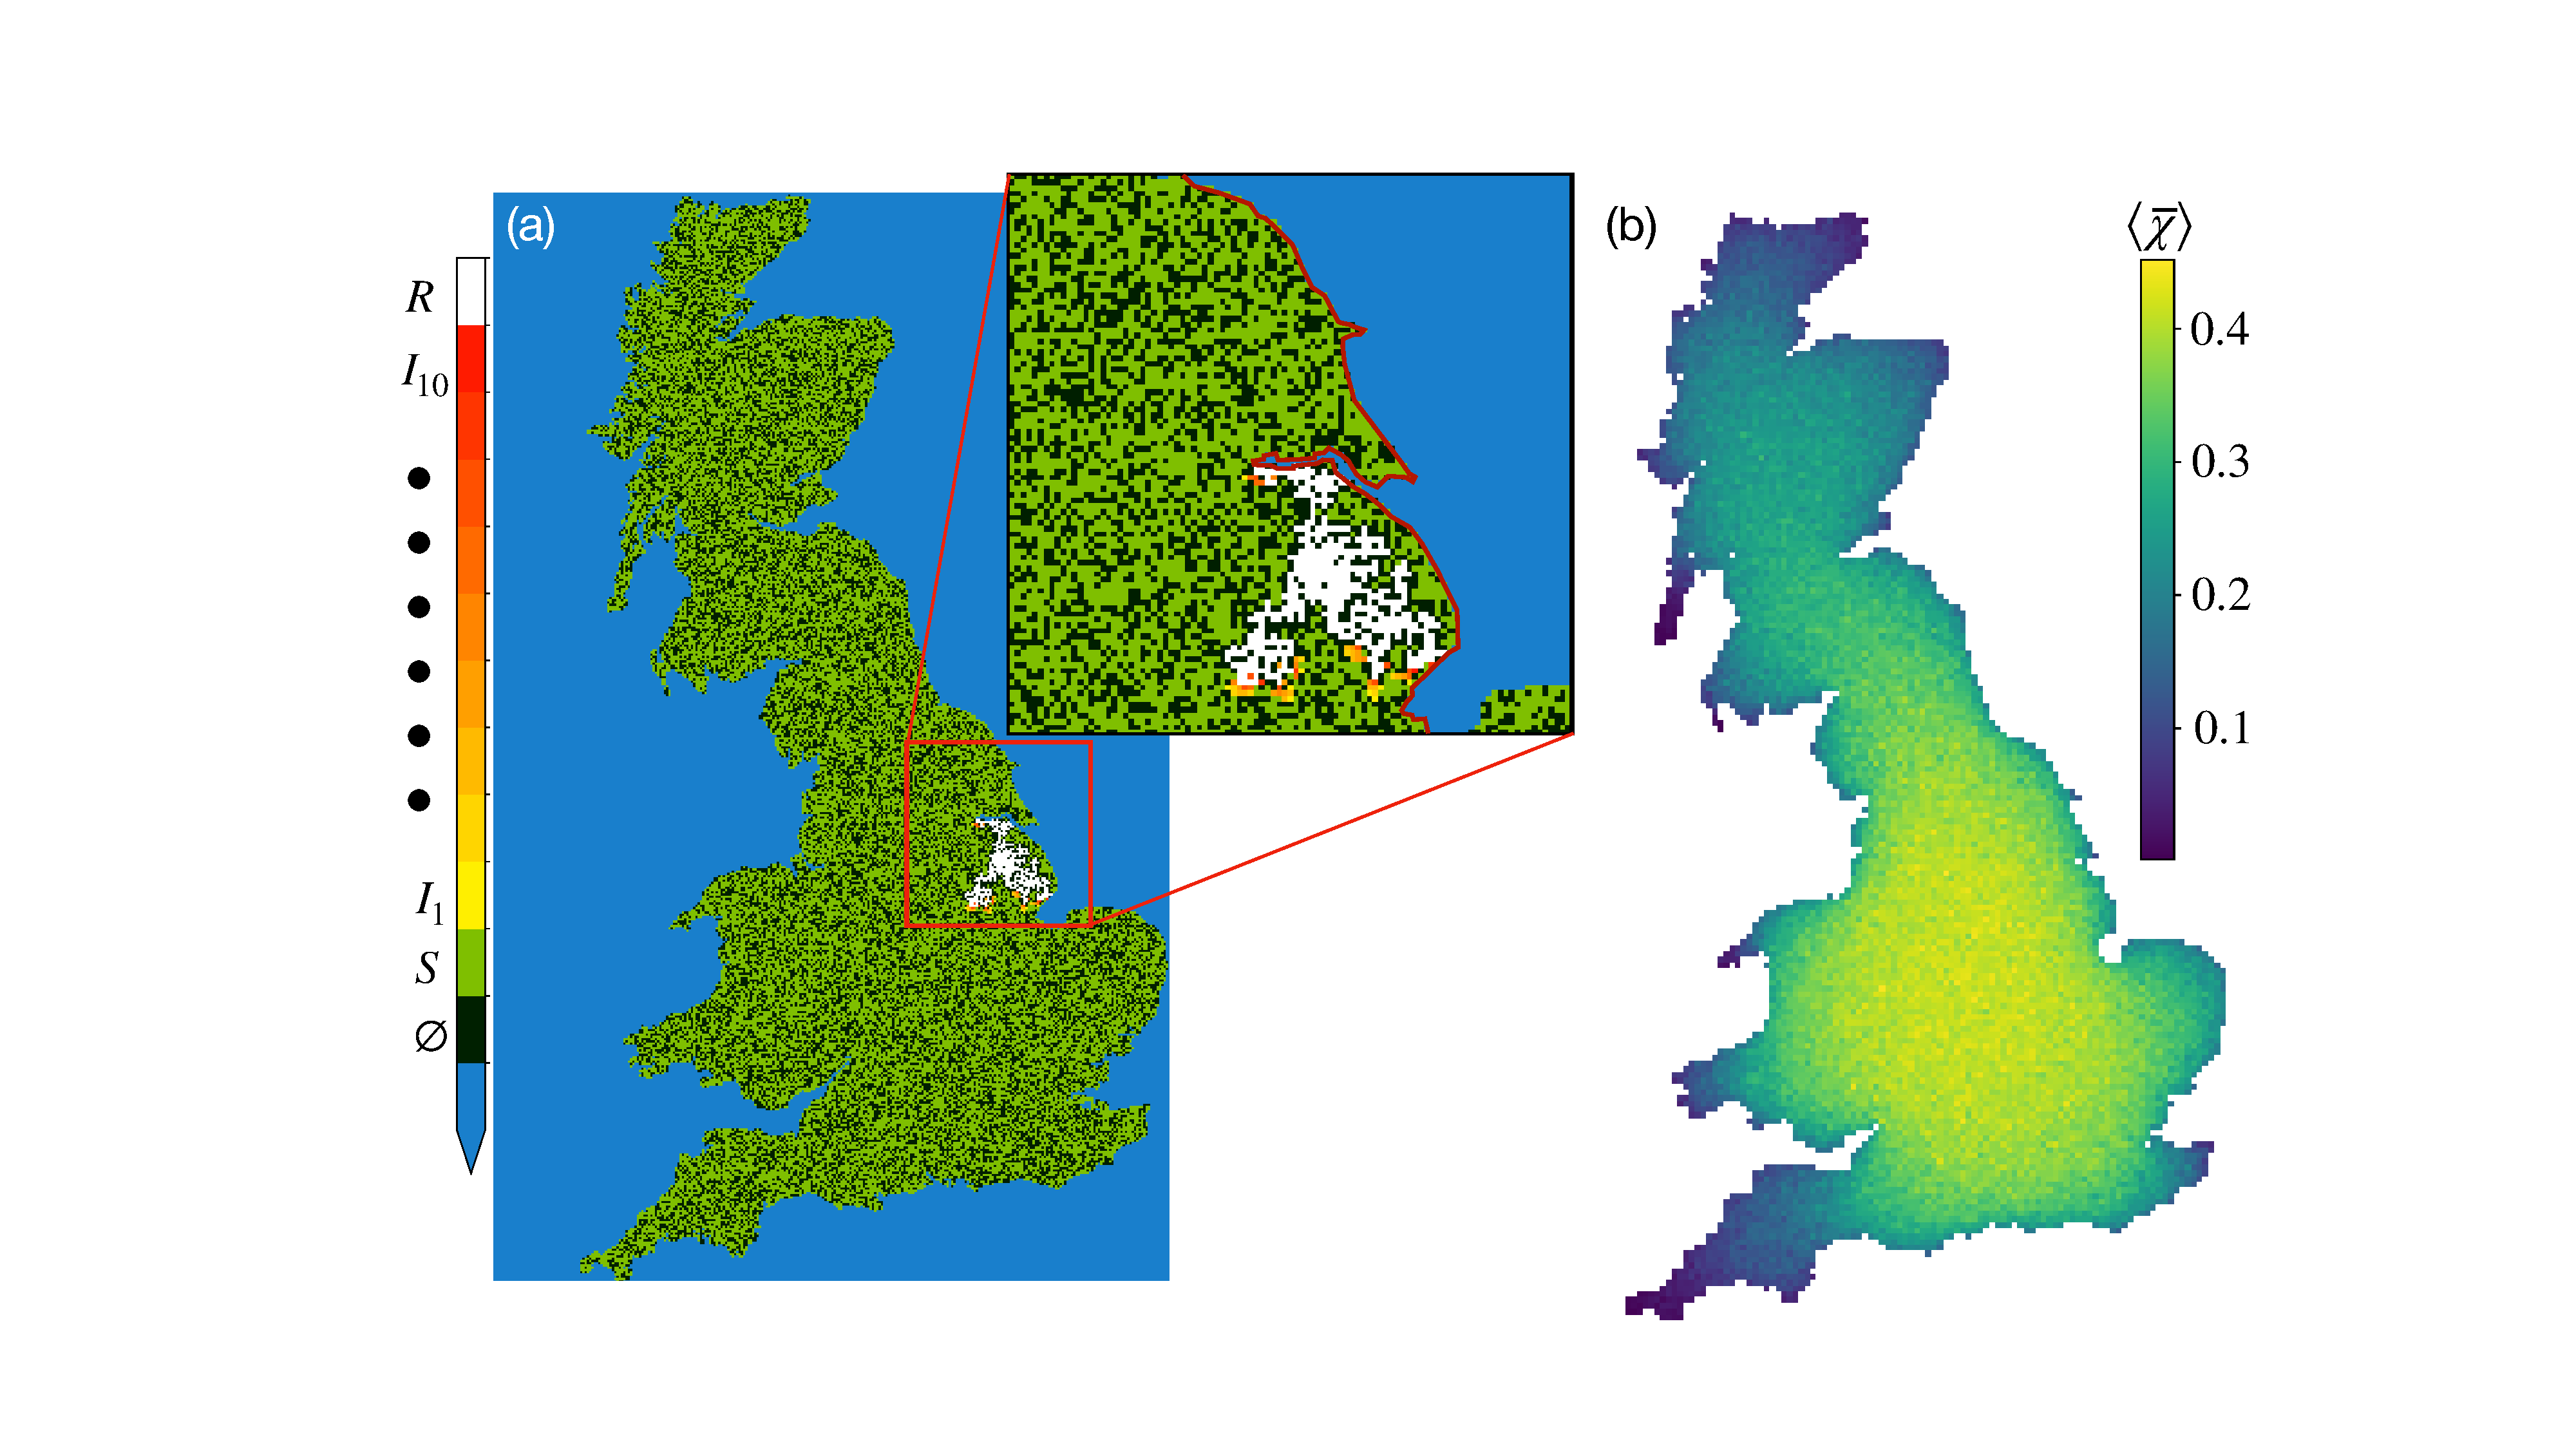
\includegraphics[scale=0.32]{chapter4/figures/figure1-GB-BCs.pdf}
    \caption{(a) The SLM spreading on a map of GB. The domain geometry and epicenter %
    location are non-trivial aspects likely to influence the spread of disease. The zoomed inset %
    shows an example of the Humber estuary preceding an infectious wave-front. 
    (b) Ensemble-averaged mortality-ratios are shown by colour for each spatial location with 
        parameters $\rho=0.65$ and $\beta=0.25$.}
    \label{fig:uk-spread-primer}
\end{figure}

In Figure \ref{fig:uk-spread-primer}(a), we see that coastline edge effects
might reduce the probability of an epidemic.
For example, epidemics emanating from epicentres located just below the 
Humber estuary (shown on the inset) could encounter more impedance when 
compared to more centrally-located positions.
Accordingly, SLM edge effects and domain BCs were examined by assessing the 
tree mortality from every possible epicentre, as shown in Figure \ref{fig:uk-spread-primer}(b).

Figure \ref{fig:uk-spread-primer}(b) reveals the ensemble-averaged mortality 
ratio, denoted by $\chi$.
The toy landscape-level SLM assumed parameter values just above threshold in a $2D$ square lattice. 
Each simulation began from a single patch epicentre, located at position $(i, j)$).
Here, the mortality ratio captures the total epidemic impact, defined by: 
\begin{equation}
\label{eq:epi_impact}
    \chi=\frac{R_f}{S_0}
\end{equation}
where $R_f$ is the final number of patches in the removed state at $T_f$ and $S_0$ is the number of susceptible %
patches at time $T=0$.
Given the system stochasticity, it is necessary to repeat simulations for each epicentre %
and calculate $\overline{\chi}$. Iterating over the whole of the GB in this way permits visualisation
of the spatial-susceptibility of the pathogen $\beta$, depicted by colour in Figure \ref{fig:uk-spread-primer}(b).

Figure \ref{fig:uk-spread-primer}(b) shows the result of the ensemble averaging $\chi$ for each
patch of land\footnote{Ensemble averaging each patch of land was computationally intensive, 
to account for this, the domain resolution was coarse-grained to $\mathrm{5km \times 5km}$ sized-patches.
Simulations were conducted on the Leeds high-performance computing facility, the ARC-HPC system using a task %
array, the ensemble took approximately two hours on $25$ cores.).} 
As expected, the domain BCs and map geometry change the resulting epidemic scale, 
mainly Scotland north of the Anglo-Scottish border and the south Eastern leg of GB towards Exeter and Plymouth;
meanwhile, centralised regions show a roughly constant susceptibility. 
Interestingly, higher epidemic parameters increased the mean mortality ratio and reduced spatial variations
in the mortality ratio, whilst lowering epidemic parameters had the opposite effect.
Although Figure \ref{fig:uk-spread-primer}(b) paints an ideal epidemic scenario involving one infected patch at $t=0$,
we can assume an emerging epidemic within the SLM model depends strongly on the interplay of epicentre location and domain boundary.
 
 \newpage

\subsection{Realistic abundance data}

In Figure \ref{fig:uk-oak-l.hill}(a), the distribution of oak is given by \cite{hill.data} is
plotted over a map of Great Britain, alongside with its corresponding 
probability density function (PDF) in  Figure \ref{fig:uk-oak-l.hill}(b).
Each pixel in Figure \ref{fig:uk-oak-l.hill}(a) depicts the predicted hectares
of oak canopy cover per kilometre squared of land, $\mathrm{ha/km^{2}}$, represented by colour. 
Therefore, each measure of abundance correlates to host density\textemdash
justified by the fact that $100\mathrm{ha} = 1 \mathrm{km^2}$\textemdash expressed as $\rho$.
The spatial map displays visual irregularities and population heterogeneity.

The PDF, $f(\rho)$, displayed in Figure \ref{fig:uk-oak-l.hill}(b) 
reveals that most land patches occupy lower canopy cover values.
Although, a small number ($\sim 5\%$) of high abundance values in the range
$10<\rho<35\ \mathrm{ha/km^2}$ that skewed the distribution were reduced to $10\mathrm{ha/km^2}$, 
thus capping the highest value to $10\%$ of oak canopy cover. 
The PDF describes a continuous distribution in opposition to the binary-valued distribution of hosts 
within the SLM. To navigate this problem, we introduce a threshold function:  
\begin{equation}
  \phi(\rho) =
  \begin{cases}
    1 & \rho_{i,j}\geq\rho \\
    0 & \rho_{i,j}<\rho
  \end{cases}
\end{equation}
where the canopy cover $\rho\in[0, 10]\ \mathrm{ha/km^{2}}$ acts as a threshold value, 
above which all patches become susceptible and assumes the numerical value of unity, i.e. $\rho < \rho_{i,j} = 1$.
Conversely, insusceptible states are described when $\rho \geq \rho_{i,j}= 0$.
The inset of Figure \ref{fig:uk-oak-l.hill}(b) visually depicts the abundance threshold function; 
the vertical black line is an arbitrary threshold $\rho$, and all canopy cover values less and greater than
$\rho$ describe insusceptible and susceptible, respectively.
Susceptible patches have enough hosts to support disease survival, growth, and spread in this interpretation. %
Patches of land below the abundance threshold are presumed insusceptible on account of insufficient hosts.

\newpage

\begin{figure}
    \centering
    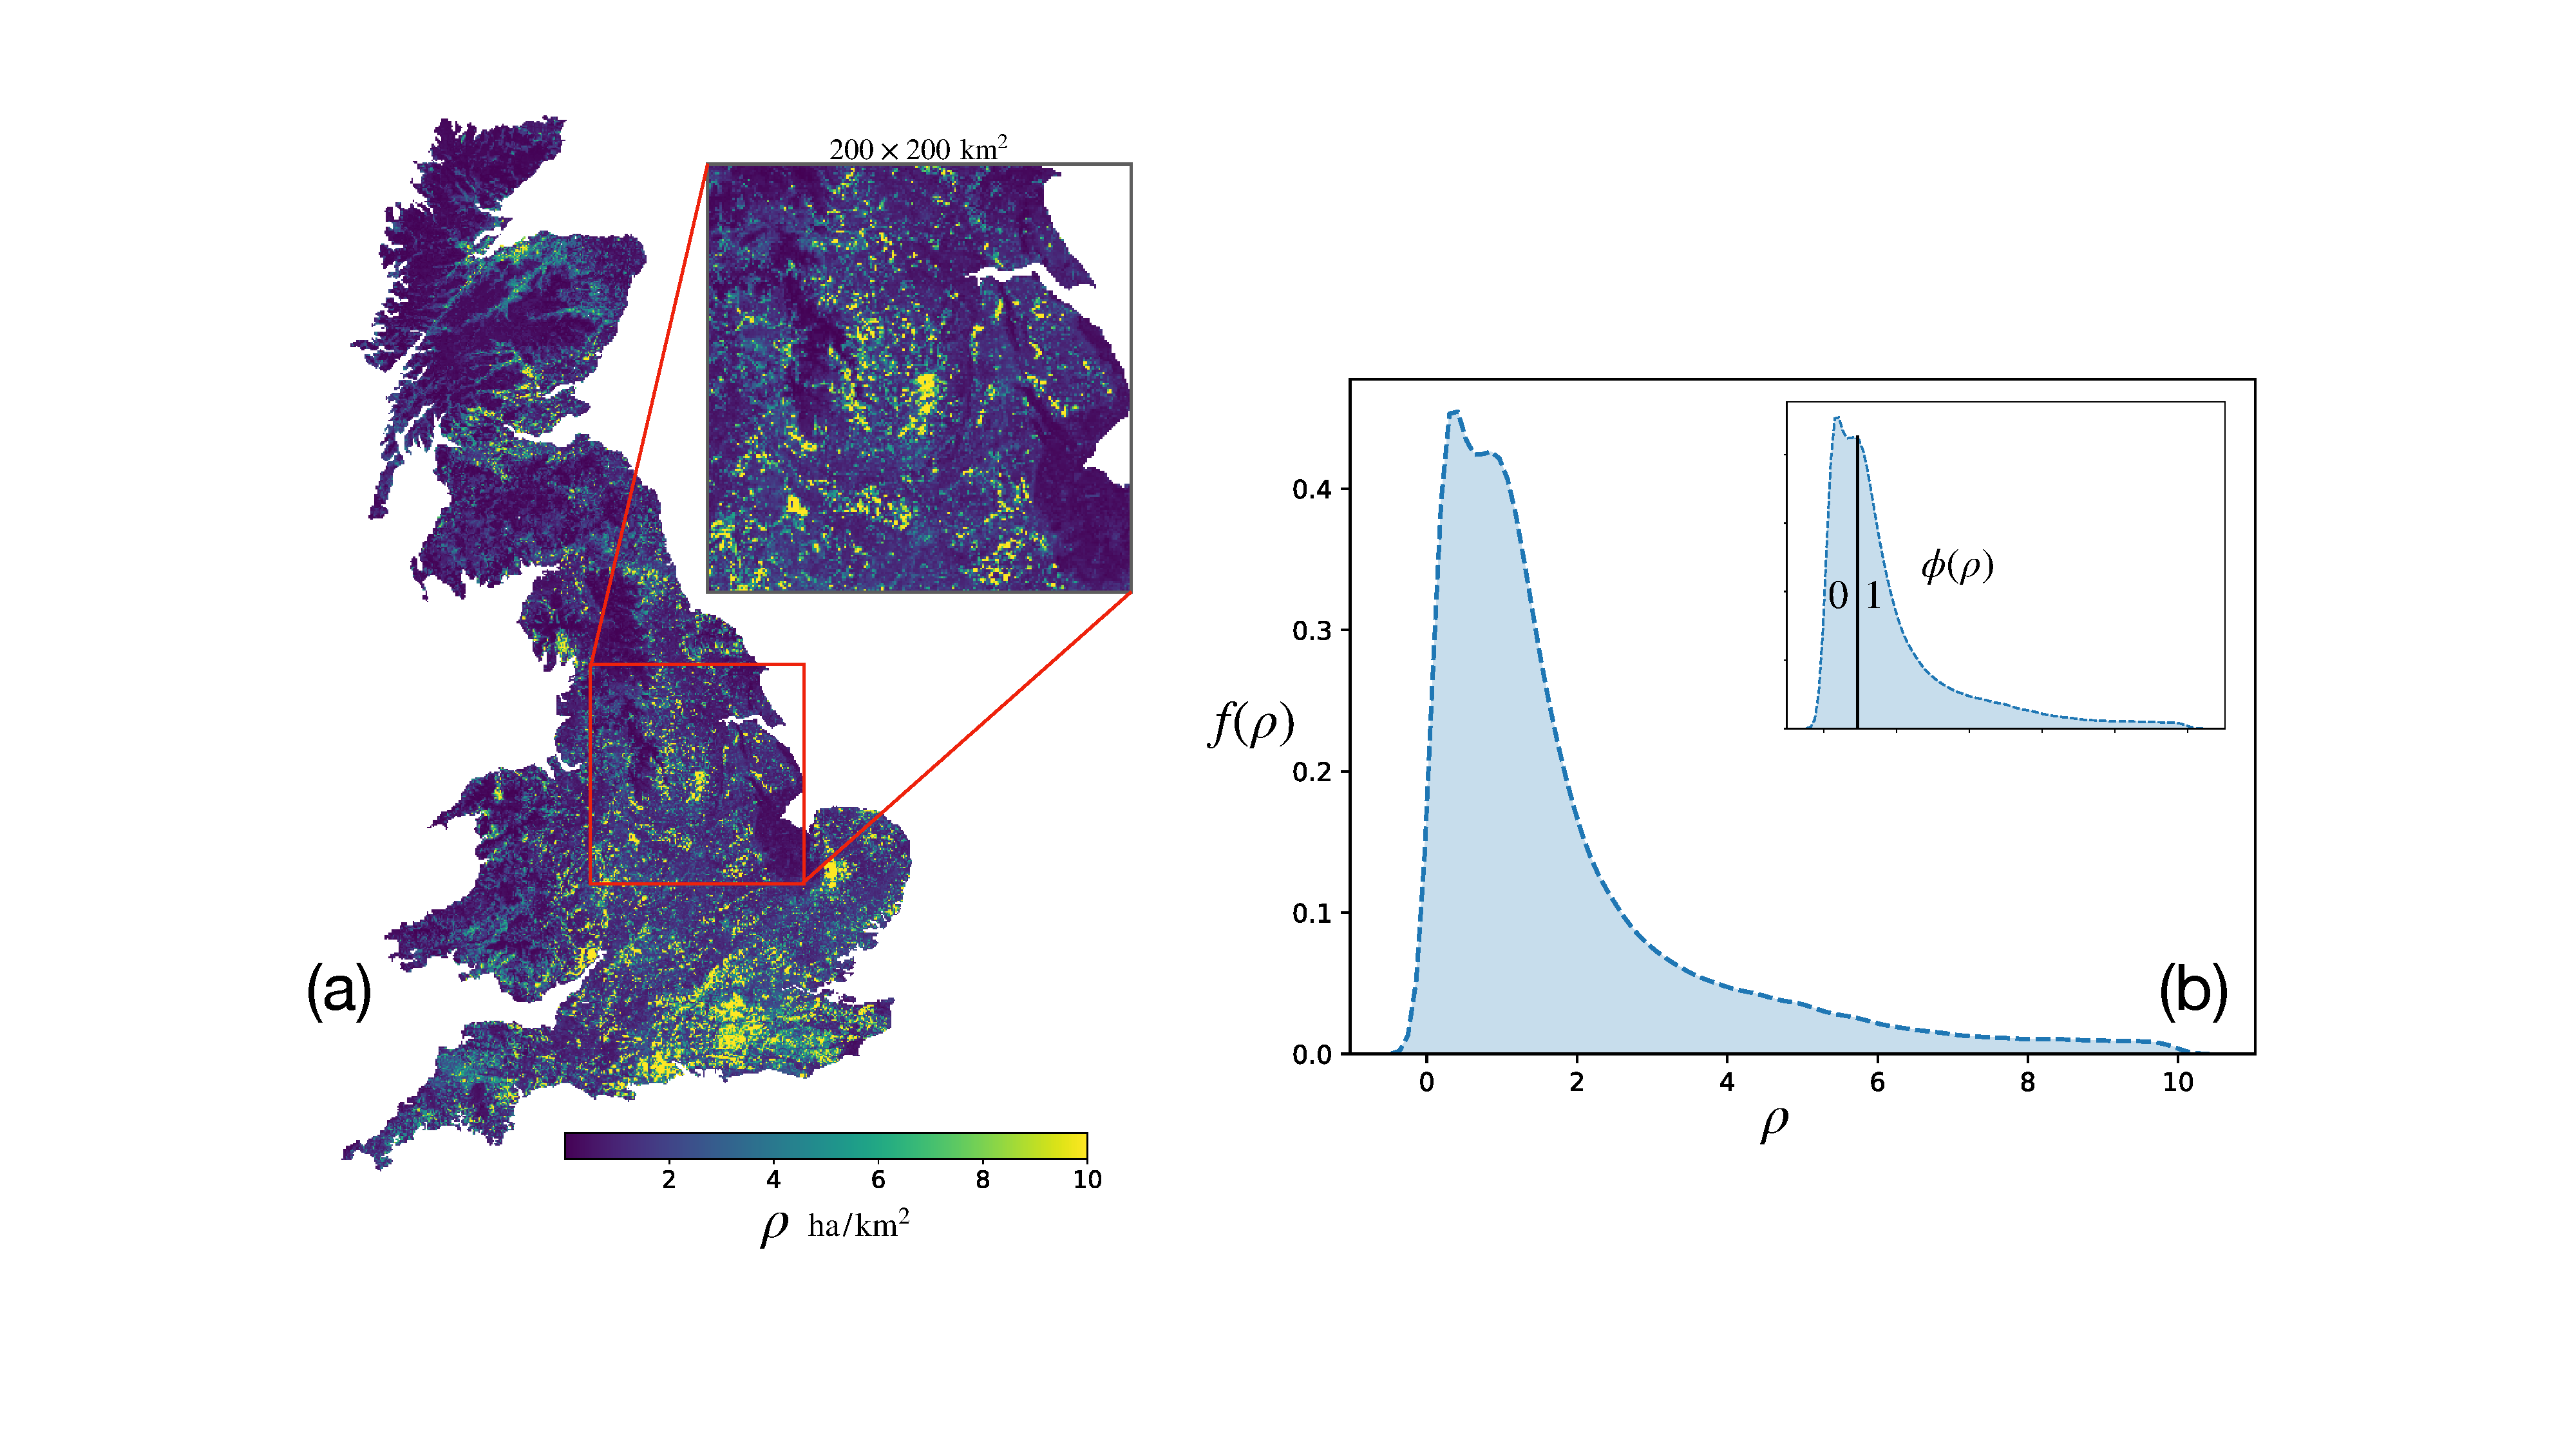
\includegraphics[scale=0.32]{chapter4/figures/figure3.pdf}
    \caption{
    (a) The modelled abundance distribution of common oak (\textit{Quercus robur}), inferred by \cite{hill.data}; each pixel holds a predicted value of abundance having units hectares of canopy cover per kilometer squared of land. 
    (b) The probability density function of abundance $f(\rho) \mathrm{ha/km^2}$. 
    The zoomed inset illustrates the process of generating threshold function $\phi$.}
    \label{fig:uk-oak-l.hill}
\end{figure}

Earlier in chapter \ref{chapter:SLM}, hosts distributions were easily characterised by $\rho \in [0, 1]$, 
describing a uniform density throughout a square lattice.
Now, however, host heterogeneity prevents a simple description of density.
Nevertheless, by considering the percentage of susceptible patches,
one can define effective landscape density $\rho^*$:
\begin{equation}
    \label{eq:rho_eff}
  \rho^{*} = \frac{\sum^{i, j} ( \rho_{i,j} \geq \rho )}{|\mathcal{L}_{GB}|}
\end{equation}
where $\mathcal{L}_{GB}$ represents host distribution over Great Britain. 
The terms $\sum^{i, j} (\rho_{i,j} \geq \rho)$ and $|\mathcal{L}_{GB}|$ represent 
the total number of susceptible patches and total landmass respectively. 
Given an increase in the threshold $\rho$, the effective density $\rho^*$ decreases; 
likewise, a decrease in $\rho$ increases $\rho^*$ as more patches become susceptible. 
Thus, $\rho^{*}$ presents a convenient, although crude, agent
to adjust the host distribution to higher or lower densities.

\subsection{Epidemics through heterogeneous landscapes}

Applying the effective density ($\rho^{*}$) of Equation \ref{eq:rho_eff},
we can initialise a set of binary-valued SLM heterogeneous domains. 
Figure \ref{fig:ch4_uk_spread} shows three variations of effective density
$\rho^{*} \in [0.40, 0.50, 0.60]$, alongside the corresponding thresholds of
abundance canopy cover shown below. In Figure \ref{fig:ch4_uk_spread}, the SLM
is simulated with infectiviy $\beta=0.25$, until pathogen extinction, 
shown through through four time-steps. Between panels (a) (e) and (i), 
the differences in the domain density are visible,
as larger values of abundance thresholds produce lower density maps.
For the three simulations shown in Figure \ref{fig:ch4_uk_spread}, 
epicentres were placed in the south, where the canopy cover is most dense. 

Previously, density was uniform in all directions, 
but now heterogeneity unevenly distributes susceptible hosts. 
Notwithstanding, we may still expect an epidemic to emerge if density 
and infectivity parameters satisfy a critical threshold, as explored in chapter \ref{chapter:SLM}.
For all $\rho^*$ values shown in Figure \ref{fig:oak-spatial-ensemble}, 
initial outbreaks ($0<t<250$) spread above the threshold.
Although at $\rho^*=0.40$, we notice a significant drop in disease progression 
beyond $t=250$ in (c-d), approximately extending from Oxford to Buckinghamshire due to a low density;
in contrast, $\rho^*=0.50$ and $\rho^*=0.60$ spread above the threshold for all panels.

In Figure \ref{fig:ch4_uk_spread} we can observe a spatial dependence in the SLM threshold,
where above-threshold regions (e.g. the in south) depend on the host density $\rho^*$ parameter.
In particular, Figure \ref{fig:ch4_uk_spread} demonstrates that increasing $\rho^*$ can lead to channels opening between different above-threshold regions, thus permitting disease to invade new regions, c.f. Figure \ref{fig:ch4_uk_spread}(d), (h), and (l) where higher density simulations spread progressively further northwards.
Undesirably, percolation is hard to define in the domain configuration shown in 
Figure \ref{fig:oak-spatial-ensemble} because the extent between borders is now non-uniform
and dependant on epicentre location.
Furthermore, simulation time series are subject to additional noise on account of heterogeneity, 
making velocity-based metrics such as Equation \ref{eq:vel_eff_r} hard to use. 
Subsequently, the examination of disease progression will focus on the mortality ratio $\chi$, 
as its measurement depends only on the final value of removed trees.

\begin{figure}
    \centering
    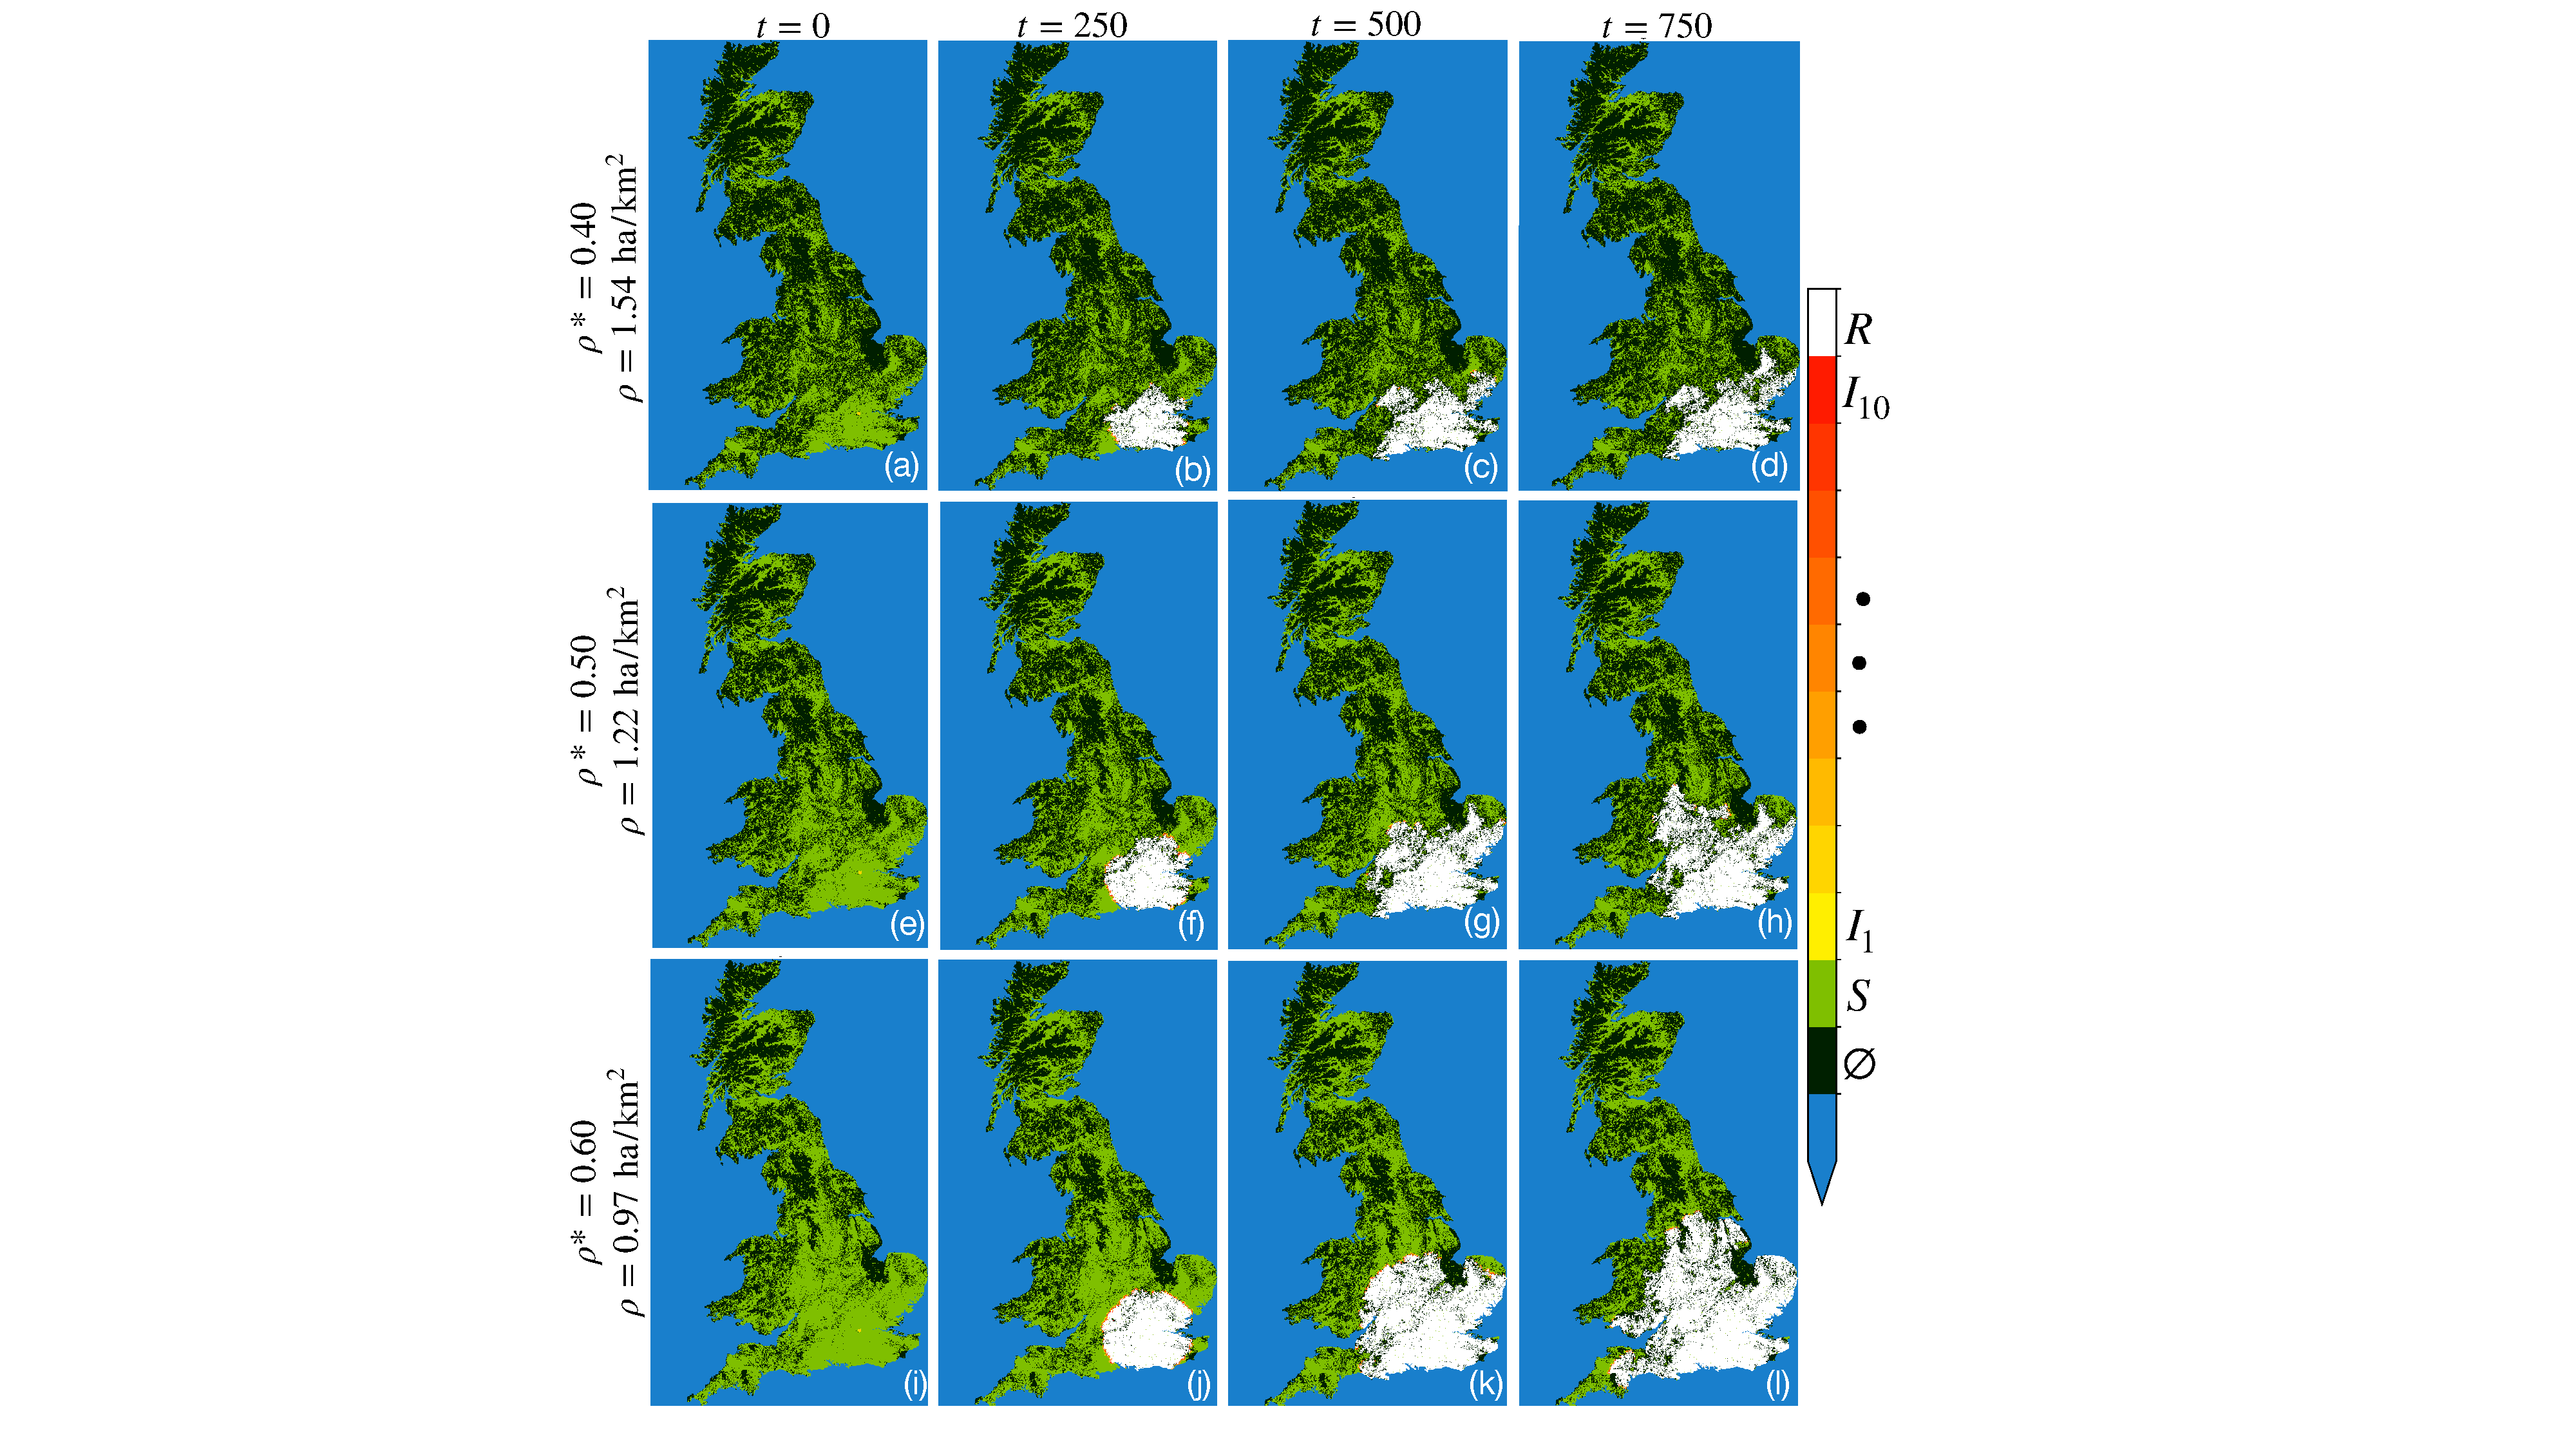
\includegraphics[scale=0.490]{chapter4/figures/figure4.pdf}
    \caption{The simple lattice model running on a binary-valued Oak domain with infectivity $\beta=0.25$ for three variations of effective density $\rho^*$.}
    \label{fig:ch4_uk_spread}
\end{figure}

\subsection{Spatially dependent ensembles}
\label{sec:slm-spatial-ensembles}

The observations of spatially varying thresholds, as suggested by Figure \ref{fig:ch4_uk_spread}, 
motivates an examination of epidemic impact as a function of epicentre location.
As such, we apply the same ensemble averaging method discussed previously (in Figure \ref{fig:uk-spread-primer})
to the oak abundance data set. That is, treating each location $(i,j)$ in GB as a potential
epicentre and ensemble averaging host mortality over many simulations.
Here, the mortality ratio $\big\langle \overline{\chi} \big\rangle \in [0, 1]$ describes the ratio 
of removed host patches to the total number of susceptible patches at $t=0$ and 
expresses the final sized epidemic in the SLM. 

The results of spatial ensemble averaging simulations are shown in Figure \ref{fig:oak-spatial-ensemble},
for three different effective densities and one value of infectivity $\beta=0.25$. 
The values of effective density in Figure \ref{fig:oak-spatial-ensemble} are arbitrary
but crucially exhibit the heterogeneous SLM behaviour. Unsurprisingly, increasing the effective density yields a 
higher mortality ratio (as defined by Equation \ref{eq:epi_impact}), thus increasing the magnitude of successive 
colour bars in Figures \ref{fig:oak-spatial-ensemble}(a-c). Alongside a more severe mortality ratio, a higher $\rho^*$
value permits disease propagation over more extensive regions, witnessed by comparing Figures \ref{fig:oak-spatial-ensemble}(a) and (c).

In Figures \ref{fig:oak-spatial-ensemble}(a-c), yellow regions highlight where the pathogen is most 
likely to spread through susceptible hosts. In this toy model, mortality is approximately independent of epicentre location, 
provided sufficient (Von Neumann) connectivity between patches, supported by uniform yellow contours within susceptible regions.
In panel (a), the spatial locations encircled in dashed red highlight a region of instability that appears to separate two susceptible regions.
In these regions, the epidemic impact could vary significantly, 
consequently prompting the corresponding plots of mortality variance in Figures \ref{fig:oak-spatial-ensemble}(d-f).

\begin{figure}
    \centering
    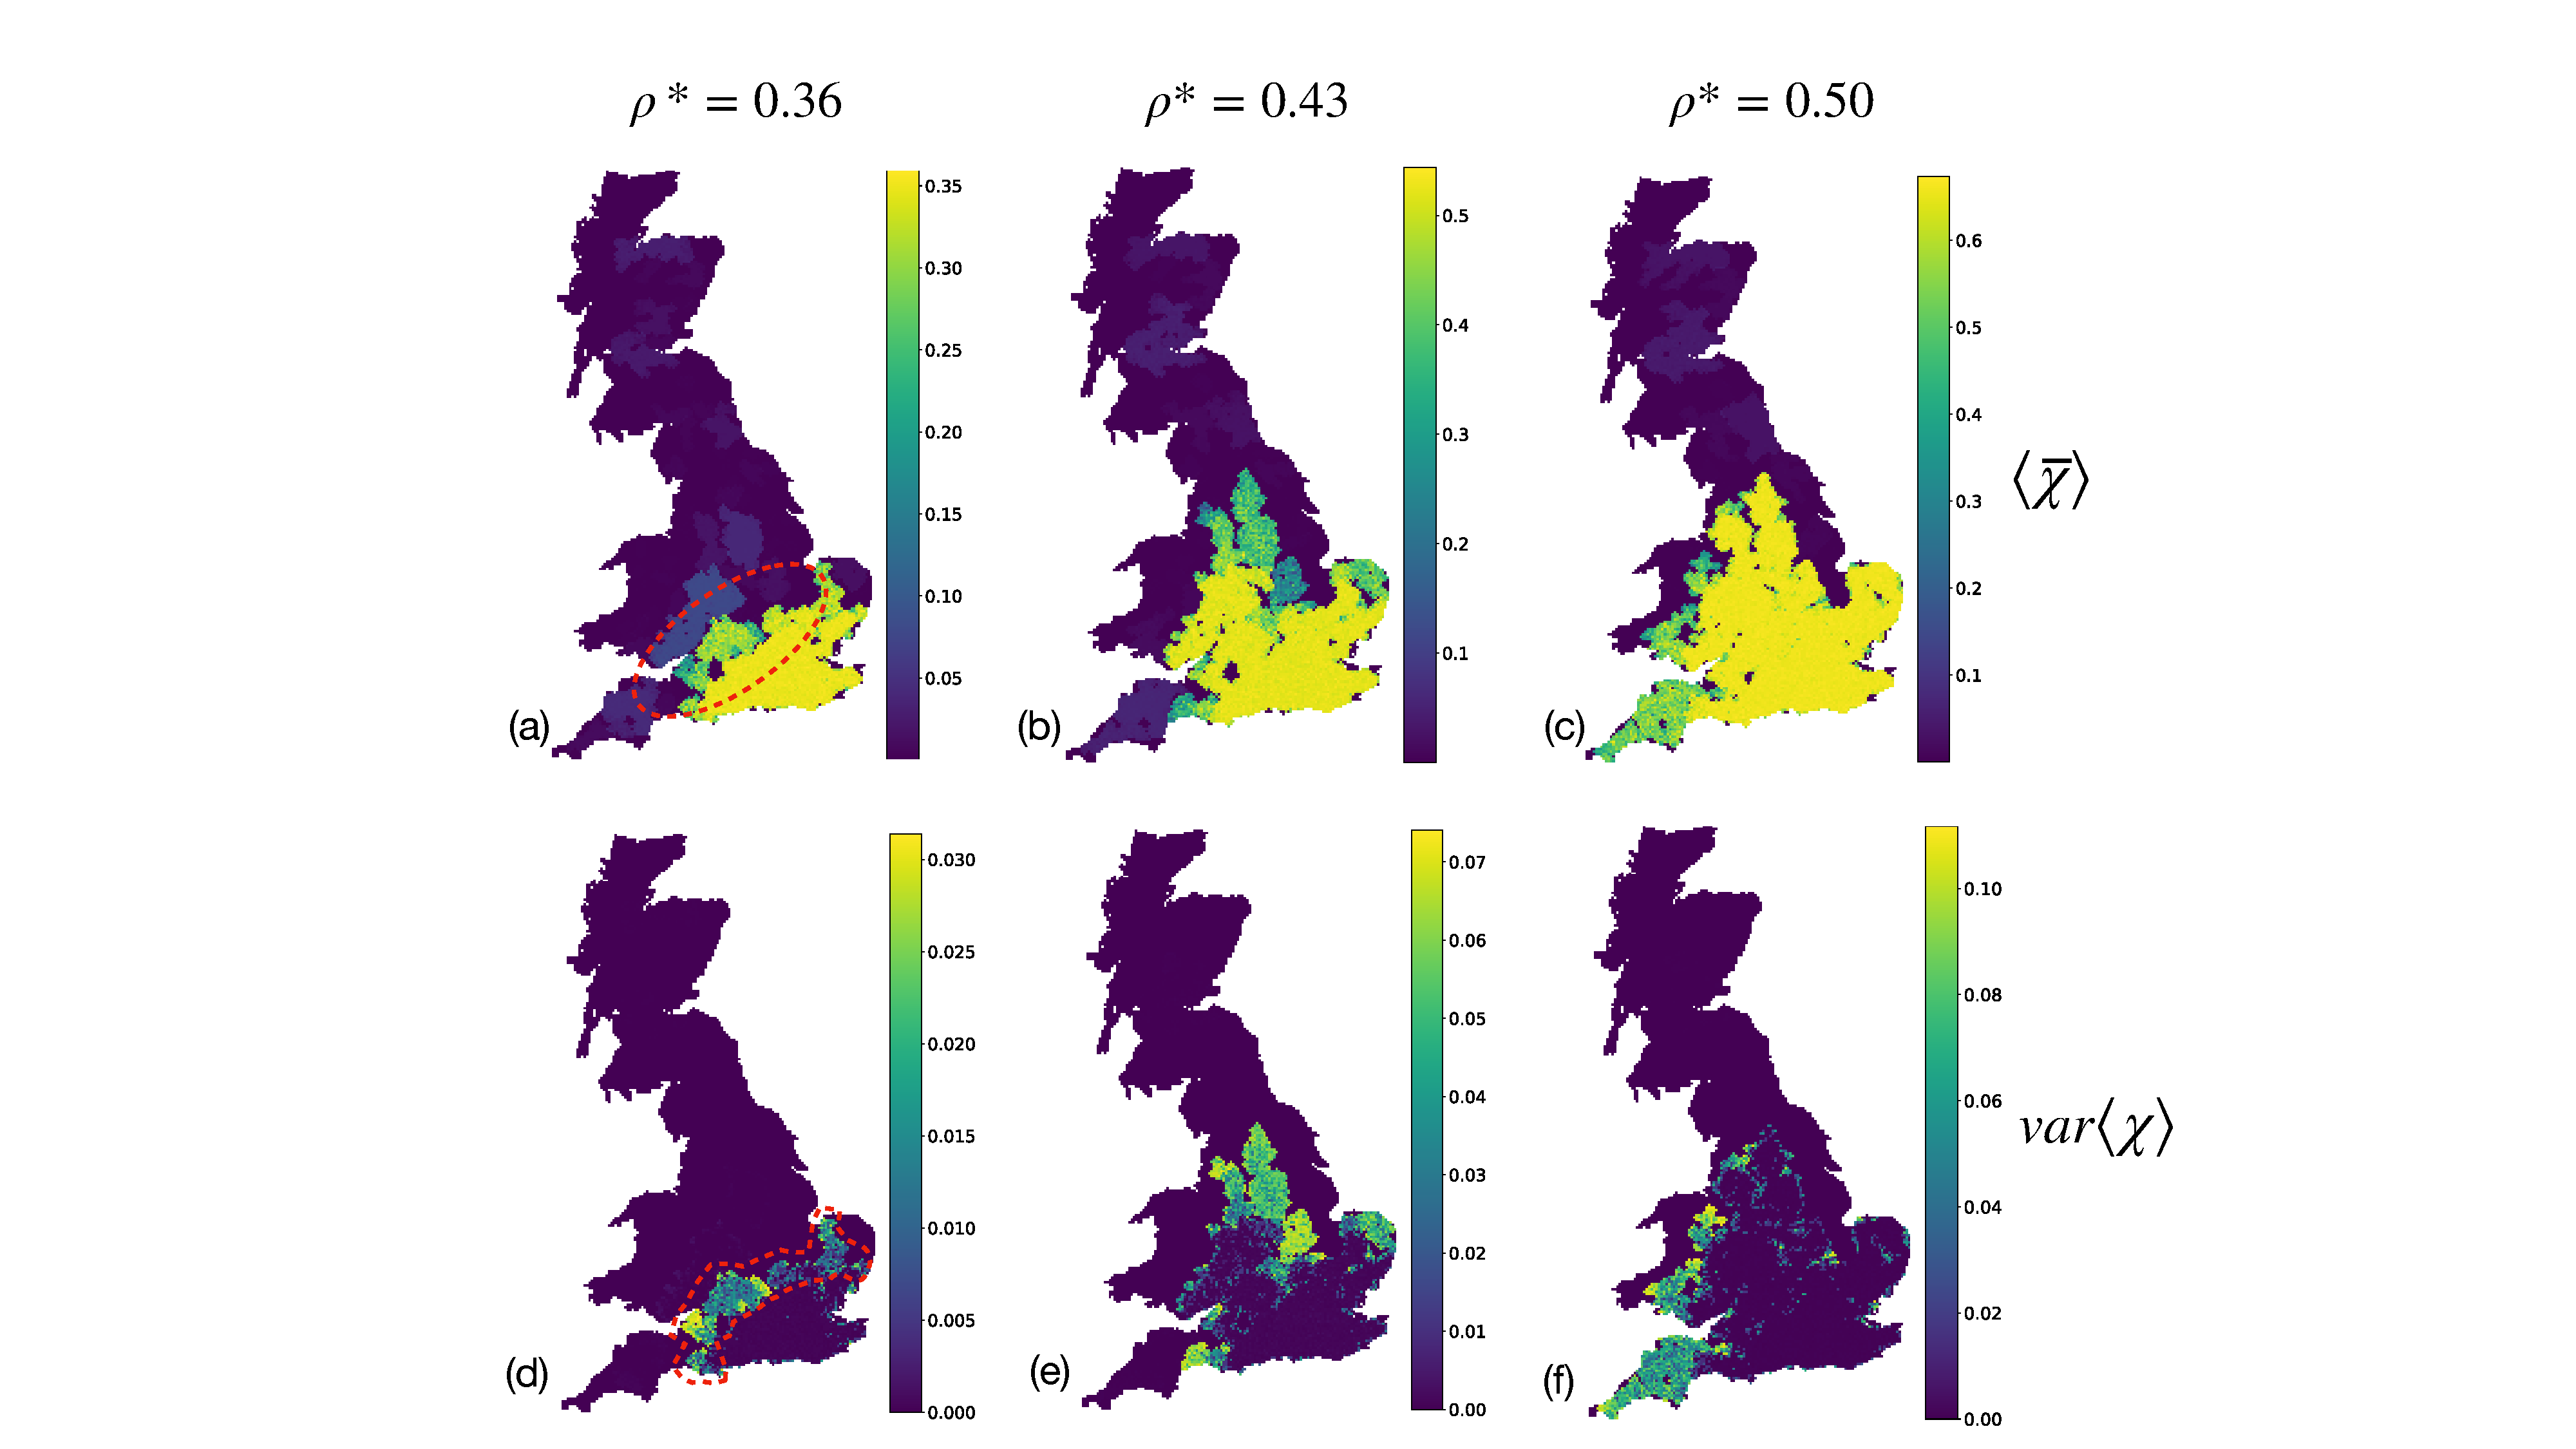
\includegraphics[scale=0.4]{chapter4/figures/figure5.pdf}
    \caption{Spatial phase showing ensemble statistics over the oak data-set for three variations of density threshold $\phi(\rho): \rho \in [0.37, 0.43, 0.50]$ and fixed infectivity $\beta=0.25$. (a-c) The ensemble mean of mortality ratio $\chi$ measured for each pixel epicenter. The dotted red circle in Fig (a) shows two neighbouring susceptible regions. (d-f) Ensemble variance over $\chi$. The dotted shape in (d) highlights an unstable region of high variance and uncertainty separating two susceptible areas of the population in Fig (a).}
    \label{fig:oak-spatial-ensemble}
\end{figure}
Plotting the mortality ensemble variance illustrates where epidemic outcomes can go either direction, 
where the possibility of large-scale epidemic and pathogen extinction exists simultaneously in the parameter regime.
Figure \ref{fig:oak-spatial-ensemble}(d) captures a centrally-located region of uncertainty, highlighted in red; 
in these regions, the toy model may or may not give rise to a large scale epidemic, as opposed to the most southerly, 
high-mortality region beneath the dashed red lines. Panels (e) and (f) show a variance only in the edges of the centrally
located susceptible region. It is alluring to consider the implications of high variance regions in Figures \ref{fig:oak-spatial-ensemble}(d-f)
in the context of epidemic control. Namely, we may suppose that epidemic control through high variance regions could be an effective strategy
in stopping the spread of disease.
Although the mortality ratio ($\chi$) categorises the overall epidemic scale in the SLM, 
it fails to reflect any information about how far an epidemic is likely to propagate.
Recording the maximum distance travelled by the pathogen proved a helpful method to illustrate spatial progression,
maps of `maximum distance' are displayed in appendix \ref{a:landscape-toy-model}. 


\subsection{Heterogeneous parameter sweeps}

Ensemble analysis has so far fixed infectivity to $\beta=0.25$
and instead concentrated on mapping mortality with a varying effective density parameter $\rho^*$.
In this section, we investigate the entire parameter space of $\rho^*$ and $\beta$.
Figure \ref{fig:heterogeneous-phase-space} depicts a full parameter sweep of the toy landscape SLM.
Due to more host units in computer memory, simulating the spread of disease in the toy landscape SLM is more 
computationally challenging when compared to the ideal square SLM in chapter \ref{ch3:two-param-model}.
Even though epidemic progression in the SLM is conditioned on epicentre location (as confirmed by the findings of section \ref{sec:slm-spatial-ensembles}),
analysing a single epicentre is sufficient to capture the essential toy model behaviour.
Ergo, we present an analysis through a single epicentre.

Figure \ref{fig:heterogeneous-phase-space} shows the ensemble-averaged epidemic phase space of the toy landscape SLM
through a epicentre\textemdash indicated by the red point in Figure \ref{fig:heterogeneous-phase-space}(a).
The Parameter sweeps of $\rho^{*}$ and $\beta$ demonstrate multiple discontinuities and sharp increases in $\chi$
for particular combinations of $\rho^{*}$ and $\beta$; this contrast with the parameter sweeps inside a homogeneous square domain.
Moreover, Figure \ref{fig:heterogeneous-phase-space}(b) reveals a large asymmetry between $\rho^*$ and $\beta$ 
as more discontinuous jumps appear most when $\rho^*$ is increased, i.e. moving horizontally 
through Figure \ref{fig:heterogeneous-phase-space}(b). Hence, host heterogeneity gives rise to distinct behaviours for both
$\rho^*$ and $\beta$ axes, as opposed to the (approximately) symmetric ensembles in a homogeneous square domain.  

Figures \ref{fig:heterogeneous-phase-space}(c-d) contrast behavioural differences between 
$\rho^*$ and $\beta$ axes. Specifically, we compare one-dimensional slices through both parameters $\rho^*$ and $\beta$.
Figure \ref{fig:heterogeneous-phase-space}(d) details how variations of $\rho^*$ effect the model behaviour through $\beta$-space. 
Interestingly, Figure \ref{fig:heterogeneous-phase-space}(d) depicts the same infectivity threshold of $\beta\sim0.10$, 
identical to the SLM evolving on a uniform square domain. When $\beta$ increases, fewer discontinuities arise when
compared to $\rho^*$, as evidenced by smoother curves. 

For each value of density in Figure \ref{fig:heterogeneous-phase-space}(d), 
the mortality remains fixed beyond $0.30 \lessapprox \beta$.
We may understand the independence between $\chi$ and infectivity through a numerical example:
the probability of a susceptible patch remaining susceptible when it encounters 
an infected neighbour is given by Equation \ref{eq:pr_s_s} as $Pr(S \rightarrow S) = (1 - 0.30)^{10} = 0.03$. 
Therefore, on average the pathogen transmits successfully to susceptible neighbours with probability $Pr(S\rightarrow I)=0.97$, 
e.g. if a particular epicentre belongs to a susceptible region containing $100$ patches, only three patches remain susceptible. 
In this instance, most patches in the cluster become infected, and further increases in $\beta$ do not affect the 
mortality\footnote{
Increasing the infectivity to $\beta=0.40$ yields a $Pr(S \rightarrow S) = 0.006$, 
leading to negligible changes in the final epidemic size\textemdash however, the rate of progression is still faster.
}. 
When $0.30 \sim \beta$, only increases to the domain density have the potential to raise the final epidemic size, 
indicated by the increases in the height of the curves in Figure \ref{fig:heterogeneous-phase-space}(d). 

\begin{figure}
    \centering
    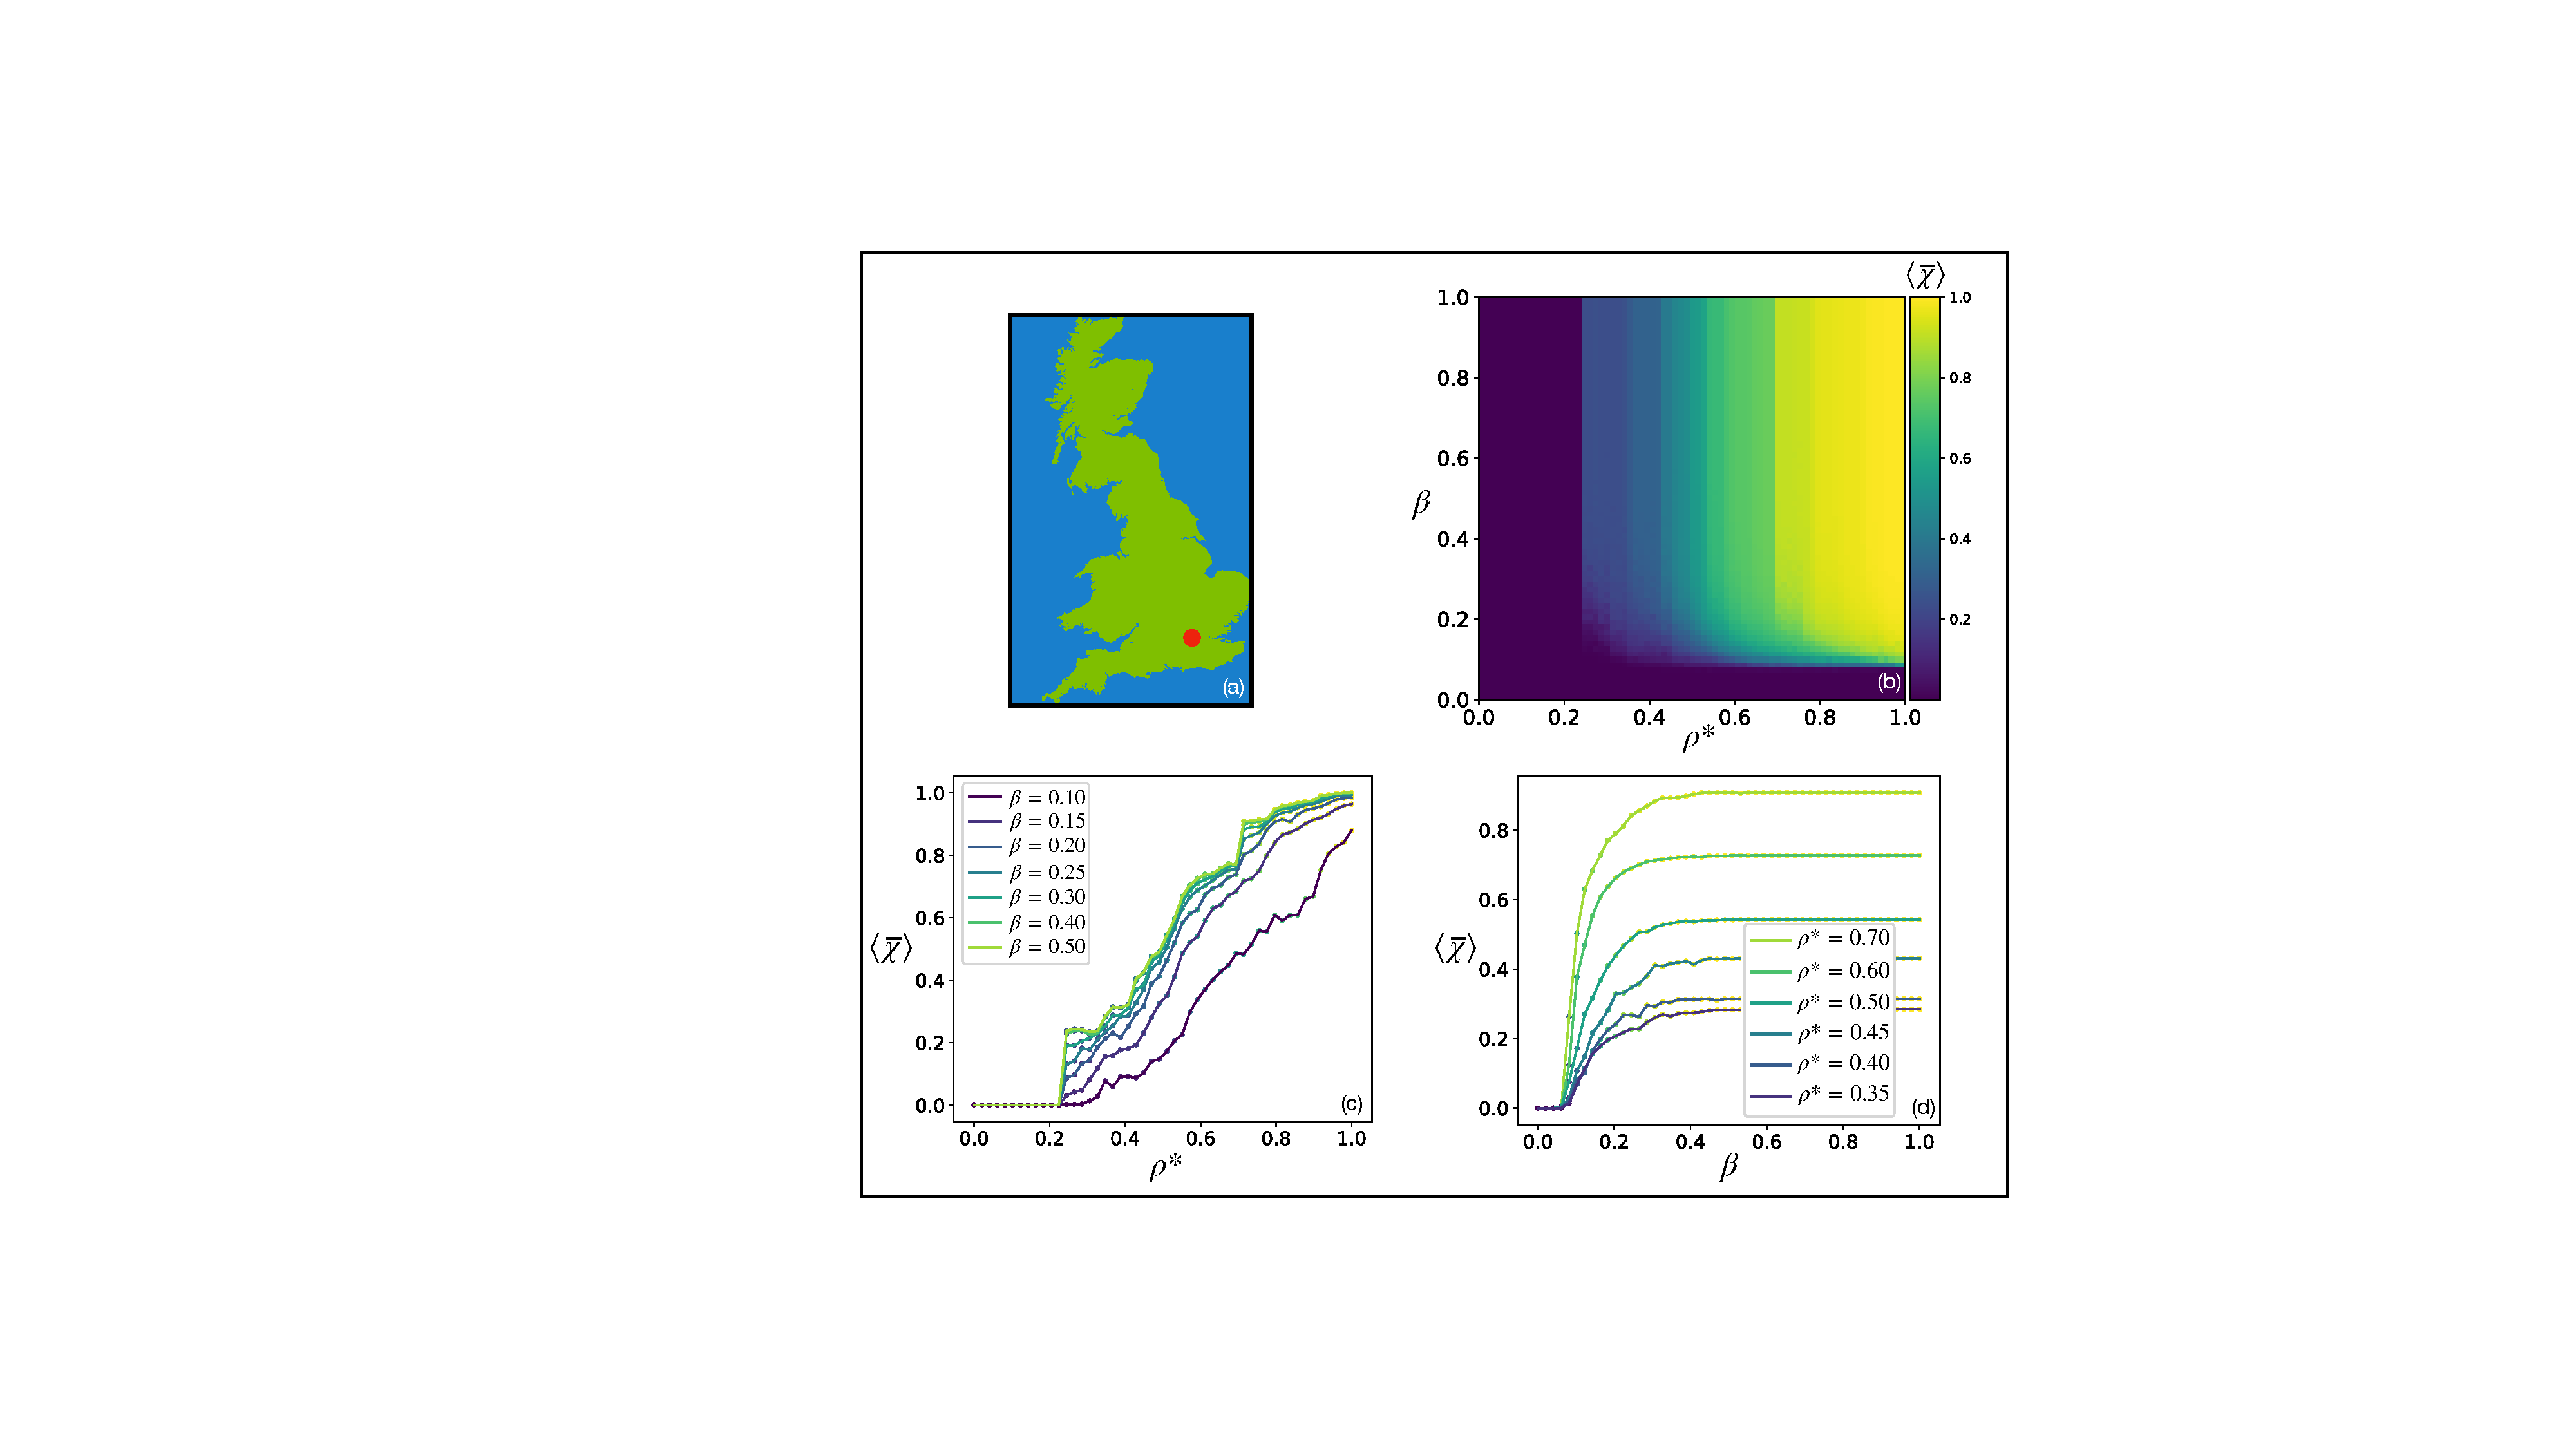
\includegraphics[scale=0.55]{chapter4/figures/figure4-param-sweeps.pdf}
    \caption{
    Beginning from a single fixed epicentre, shown in red inside panel (a),
    ensemble-averaged parameter sweeps of the toy model display a threshold-like behaviour.
    (b) The mortality ratio is plotted over the two-dimensional parameter space of $\rho^*$ and $\beta$. 
    (c) A one-dimensional plot of mortality as a function of host density is shown alongside several slices of infectivity, indicated by colour.
    (d) The mortality ratio is found over infectivity $\beta$ for different values of effective density $\rho^{*}$.
    }
    \label{fig:heterogeneous-phase-space}
\end{figure}

\newpage

\section{Discussion}

In this chapter, we explored two applications of the SLM viz; early warning signals and a toy landscape-level model.
The original analysis conducted by \cite{OROZCOFUENTES201912} relied on a velocity metric based on the number of 
infected and removed trees, $N_I$ and $N_R$ respectively. In this scheme, the number of infected and removed hosts scales as
$\propto (N_I + N_R)^2$ above the threshold, giving rise to an effective increase in velocity for later times;
as we discussed, these undesirable artefacts of domain geometry lead to confusing increases in the time series velocity, 
despite a constant rate of progression. Therefore, EWS were detected using an alternate (COM) time-series metric and abstract 
cylindrical domain configuration that negated geometrical effects.
A two-dimensional investigation was undertaken, sweeping the entire parameter space of tree density $\rho$ and infectivity $\beta$.

After setting up the EWS framework, the two-dimensional parameter sweep revealed that preemptive EWS detection is more obtainable 
when infectivity is lower. Observing these asymmetries in EWS detection, conditioned on infectivity
$\beta$, highlights the possible challenge of preempting progressively infectious pathogens;
in particular, given that host susceptibility is likely to increase as a consequence of climatic stressors \cite{garrett2006climate}.
Subsequently, we may hypothesise the heightened challenge of early warning indicator detection for forest-based pathosystems in the face of climate change.

EWS have found applications in a variety of ecological processes, 
e.g. aquatic ecosystem function \cite{kramer1991aquatic}, forest desertifications \cite{yang2005desertification}
and species-level extinctions \cite{drake2010early}.
Nevertheless, few sources focus explicitly on EWS from tree epidemics, akin to the dynamic (velocity-based) 
approach used by \cite{OROZCOFUENTES201912}. Instead, most research has focused on the more general class of forest
health and tree mortality\footnote{ 
See \cite{torres2021role} for a related review on remote sensing technologies and forest-health
} based on tree growth rings \cite{rogers2018detecting, mamet2015tree}. 
As such, the EWS method presented in section \ref{sec:EWS} differs from the wider literature,
and more work need to be done to scrutinise the utility of dynamic, velocity-based, EWS detection methods.

Secondly, we constructed a toy landscape-level SLM spreading through an example distribution oak, as generated by \cite{hill.data}.
The model of landscape-level epidemics neglects several essential features of invasive disease; most importantly, 
it inherited the nearest neighbour contact assumption, as discussed in chapter \ref{chapter:SLM}.
Hence, we labelled the landscape-level interpretation a`toy' model.
Although many limitations underpin the toy model (e.g. the omission of long-distance dispersal \cite{long-range-dispersal}
and cryptic infections \cite{gilligan2007impact}), it highlighted the inability of the SLM to describe the spread of disease
through lower tree densities ($\rho \in [0.01, 0.10]$), typical throughout GB.

As the SLM could not describe the spread of disease through more realistic host densities, 
we introduced an effective density parameter $\rho^*$, predicated on an arbitrarily chosen threshold.
Introducing an additional density threshold parameter is undesirable, unnatural and speculative.
Therefore, in the proceeding chapter, we are motivated to change direction and construct a non-local
dispersal model, in line with more contemporary dispersal-based approaches such as \cite{parnell2009optimal, meentemeyer2011epidemiological}.
In this paradigm, transmission between trees can occur over larger length scales and permit the spread over lower tree densities. 

Notwithstanding the inherent toy SLM shortcomings, its construction demonstrates the use of a novel modelled abundance
dataset provided by \cite{hill.data};
the modelled data is partly generated but combines various data sets\footnote{
Including ancient woodland shapefiles, BSBI distribution database, Countryside Survey data, myForest and the National Forest Inventory Great Britain 2014},
as we reviewed in section \ref{ch2:hostdata}.
However, statistically regressed (modelled) abundance data contains uncertainties and 
inaccuracies alongside the loss of small-scale host spatial structure $<1\mathrm{km^2}$.
As argued by \cite{13-challenges}, capturing host spatial structure, even when data are limited, 
is essential, and methods are required to assess the impact of incomplete or inaccurate host data.

Following this argument, host data accuracy presents a notable assumption in the toy model.
Be that as it may, density parameter sweeps over GB (as shown in Figure \ref{fig:heterogeneous-phase-space}) could 
form a simple procedure to assess the effect of host error, i.e. contrasting epidemic outcomes between two upper
and lower density error bounds. Evaluating landscape-level parameter-sweeps are uncommon, 
and most large-scale models repeat simulations over numerous control scenarios and rest on 
fitted parameters e.g. \cite{large-scale-control, doi:10.1111/j.1365-3059.2010.02391.x}.
Assessing disease outbreaks over a range of landscape-level densities parameters could describe a risk-based approach,
as articulated by some authors investigating epidemics through smaller spatial scales \cite{risk-potential-control}.

\newpage

% % % 5) Introducing non-local dispersal 
\chapter{Including dispersal}
\label{ch5:dispersal-model}

In the previous Chapter, we employed a simple lattice model (SLM) based on percolation. The percolation setting provided a tractable starting place. Nevertheless, several limitations underpinned the model. Chiefly, percolation models rest on local, nearest-neighbour (NN) contacts and cannot describe epidemics at lower, more realistic tree densities ($\rho \sim 0.10$). Subsequently, this Chapter will generalise the SLM and incorporate non-local NN interactions by introducing a generic Gaussian dispersal kernel, allowing epidemics at far lower tree densities.

The thin-tailed Gaussian kernel introduced here represents an intermediate step between the NN interactions in the SLM and the fat-tailed inverse power-law dispersal present in Chapter \ref{ch:6-adb}. The ease of integrating a Gaussian kernel proved helpful when deriving an analytic expression of $R_0$, as discussed more below. Other choices of simple one parameter dispersal kernels are possible, including the slightly longer range negative exponential \cite{nathan2012dispersal}. Regardless, any developing epidemic that follows a similar ranged kernel will ultimately approximate similar spreading patterns \cite{bullock2017synthesis}.

Firstly, we will combine dispersal-based interactions within a simplistic SIR framework to construct a non-local model (NLM) of tree disease. The model behaviour is then examined under various dispersal length scales and fitted against the standard SIR to contrast disparities between spatial and non-spatial models.
After establishing the non-local dispersal model, a spatially explicit (analytic) expression for the basic reproduction number will be derived for the model, denoted by $R_0$. 

Next, we compare analytical predictions of $R_0$  against the total tree mortality, equivalent to the final-sized epidemic. Lastly, the expression of $R_0$ is scrutinised against the `actual' number of secondary infections, computed by contact-traced individual tree-to-tree infections. Notably, the analytic and contact-traced methods of calculating $R_0$ define a threshold at $R_0=1$. As before, the analysis is kept generic, with arbitrary units of time and distance, before incorporating more biological realism in the next Chapter.

\section{A small-scale non-local SIR model}
\label{section:sgm-expo}

As before, we begin with a model fixed inside a square lattice of size $\mathcal{L}$ and host units refer to individual trees. Host distributions are initialised by a Bernoulli trial with probability $\rho$ according to a binomial distribution. Thus, the probability of host occupation ($\rho$) can be seen as a tree-density parameter and interactions between hosts are modelled over a flat and randomly distributed population.
The state of a tree can be in one of three conditions: susceptible, infected, or removed (SIR).
We assume all trees are equally susceptible, and trees that become infected transition through the states $S\rightarrow I\rightarrow R$ without the possibility of recovery.

From first principles, the probability of infection at a distance $r$ can be described by an unnormalised Gaussian function $g(r; \ell)$, where $\ell$ is a distance that sets the scale of dispersal. 
If two trees\textemdash one susceptible ($S_x$) and one infected ($I_{x^\prime}$)\textemdash are separated by a distance $r=|x - x^\prime|$, then a transition probability between the states $S_x \rightarrow I_x$ can be defined by the $g(r; \ell)$ multiplied by infectivity $\beta$:
\begin{equation}
\label{eq:pr-dispersal-transition}
    Pr(S_{x} \rightarrow I_{x} ;\ I_{x^{\prime}} ) = \beta \exp\Big[\frac{-r^2}{2\ell^2}\Big]
\end{equation}
where $\beta$ is interpreted as a probability, i.e. $\beta \in [0, 1]$. 
Equation \ref{eq:pr-dispersal-transition} generalises the SLM to include non-local interactions, hence referred to as the non-local model (NLM).
Each probability of transition is assessed against a sample drawn from a continuous uniform distribution $U(0, 1)$ following a Poisson construction \cite{cook2008constructing}. 
Probabilities are then calculated for each times step while host $S_x$ 
remains susceptible, and repeated for each susceptible tree in the domain (i.e. $\forall S_x \in [\mathcal{L}, \mathcal{L}]$).
See Appendix \ref{A:combiniing-probabilities} for more information on the computational implementation. A table of parameters for the NLM is shown below in Table \ref{tab:SIR-model}.

The same uniform lifetime dynamic (used previously in the SLM) controls the period hosts remain infectious.
That is, a host transitioning into the $I$ compartment will remain infectious for $T$ time steps before uniformly transitioning into the $R$ compartment.
In section \ref{ch3:two-param-model}, the infection period was shown to alter the wave-front thickness and the threshold value of infectivity $\beta$ required for an epidemic. 
However, an arbitrary number of $T=100$ infectious time steps remains fixed throughout this Chapter.
Uniform transitions into the $R$ compartment help to keep the model simple but present an assumption that goes against the grain of more common exponential lifetime dynamics\textemdash discussed more below in section \ref{sec:SIR-fitting}.

\begin{table}
\centering
\begin{tabular}{l l l}
\hline
\textbf{Model parameter} & \textbf{Description} & \textbf{Typical value(s)}\\
\hline
$\rho$  & Tree density & $0.00 - 0.10$ \\ 
$\beta$ & Infectivity probability & $0 - 10^{-3}$ \\
$\beta^*$ & Auxiliary infectivity & $0 - 10$ \\
$\ell$ & Gaussian dispersal parameter & $ 0 - 100$ \\
$t$ & Simulation time step & $1\ \mathrm{Au}$\\
$T$ & Infectious life time & $100$  \\
$\alpha$ & Lattice constant & $1\ \mathrm{Au}$ \\
$\mathcal{L}$ & Square lattice dimension & $200$ - $2000$ \\
$R_0$ & Basic reproduction number & $0-20$ \\
$R_0^{(i)}$ & Generational reproduction number & $0-20$ \\
\hline
\end{tabular}
\caption{Parameters used in the generic NLM, time and distance are given in arbitrary units and host densities are informed from by \cite{hill.data}.}
\label{tab:SIR-model}
\end{table}

The work presented in this Chapter is purposefully kept generic, with no specific pathogen in mind.
Therefore, each Monte Carlo step through the simulation has arbitrary units of time and distance.
Nevertheless, the units of time and distance can be envisioned to be on the order of days and meters to reflect the approximate spatio-temporal scale of general tree disease.
As demonstrated later in Chapter \ref{ch:6-adb}, spatial scale within the model can be calibrated by choosing a suitable lattice constant, denoted by $\alpha$, that reflects the size of host units.

\newpage 

\section{Model behaviour}

Spatio-temporal epidemic progression within the NLM is depicted in Figure \ref{fig:sgm-evol}.
Figures \ref{fig:sgm-evol}(a-b) depict an epidemic spreading through the domain at two time steps;
simulation parameters are given by $\rho=0.01,\ \ell = 25,\ \beta = 1.0 \times 10^{-3}$ on a domain of size $500 \times 500$.
All panels in Figure \ref{fig:sgm-evol} begin from a small number of infected hosts at the domain centre at $t=0$.
A tree density of $\rho = 0.01$ approximately mirrors the median canopy coverage of a large deciduous tree distributed throughout the GB, according to the predicted oak abundance data given by \cite{hill.data}\textemdash presented previously in Figure \ref{fig:uk-oak-l.hill}.
Unsurprisingly, extending the neighbourhood of interaction to non-nearest neighbours permits an epidemic for much lower tree densities in comparison to the SLM percolation threshold studied in Chapter \ref{chapter:SLM}.

Figures \ref{fig:sgm-evol}(a-b) suggest an approximate wave-front-like behaviour, as infections spread out radially from the epicentre.
The corresponding ensemble-averages of Figures \ref{fig:sgm-evol}(a-b) are shown below in Figures \ref{fig:sgm-evol}(c-d), and confirms a travelling wave-like spread.
For 200 repeated simulations, the spatial locations of infected trees were recorded and plotted as a two-dimensional frequency distribution.
The upper and lower marginal plots of Figures \ref{fig:sgm-evol}(c-d) show the one dimensional horizontal and vertical frequency distributions, respectively.
Disease progression in Figure \ref{fig:sgm-evol}(d) reflects the radial propagation of a travelling wave and a disease gradient of approximately $\approx 3\ell$.
Thus, choosing a small value of $\ell=25$ in comparison to the domain effectively recovers the essential wave-like behaviour exhibited by the SLM.

The thin-tailed Gaussian kernel does not permit the pathogen to jump large discontinuous distances, particularly for a small value of $\ell=25$, as shown in Figure \ref{fig:sgm-evol}. Therefore, we can present an analogy to percolation provided that the ratio $\frac{\ell}{\mathcal{L}}$ is small, allowing us to calculate a wavefront similarly to the method described previously in Chapter 3. Accordingly, Figure \ref{fig:sgm-evol}(e) reveals the largest distance an infected host will likely reach over 500 steps. Boundary conditions in Figure \ref{fig:sgm-evol}(e) terminate simulations upon three conditions: 
(A) The simulation time step exceeds 500 steps 
(B) No infected trees remain in the domain 
(C) An infected tree $I_{x}$ falls within a distance $\mathcal{L} - 3\sigma_{ga} \leq I_{x} \leq \mathcal{L}$ away from the epicentre.
    
\begin{figure}
    \centering
    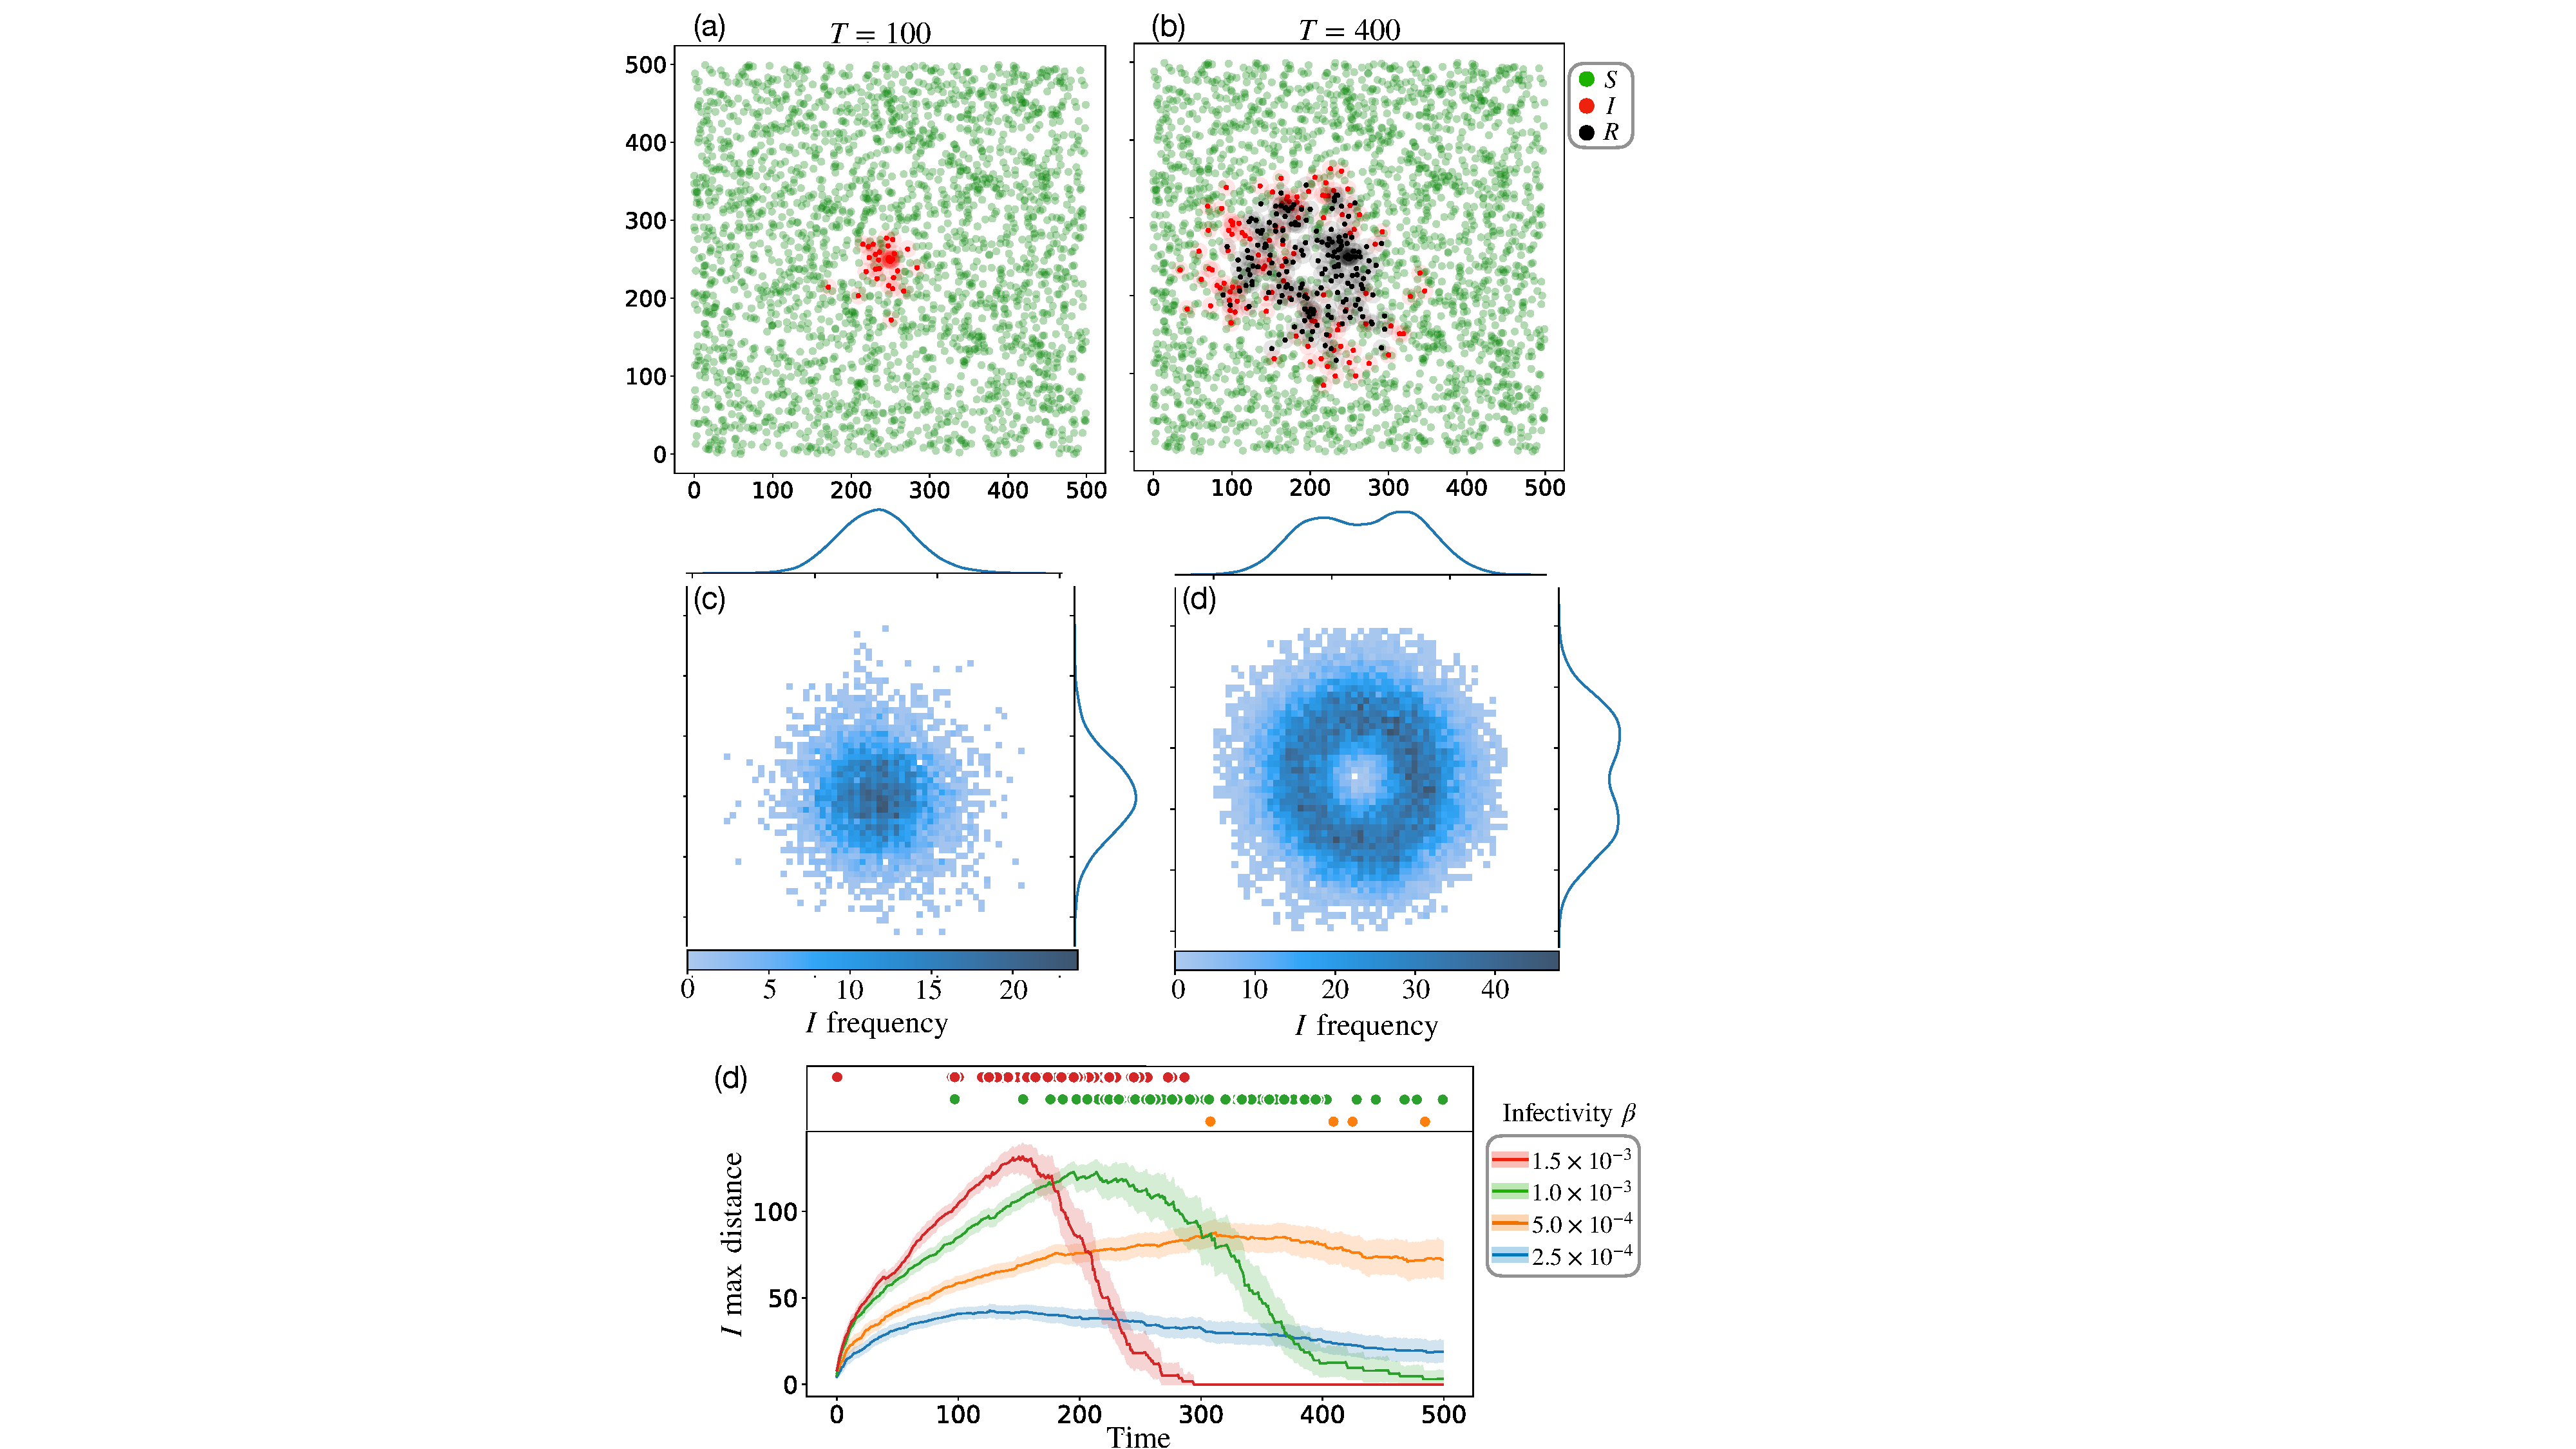
\includegraphics[scale=0.48]{chapter5/figures/fig1-sir-spatio-temporal.pdf}
    \caption{Percolation-like disease progression of the dispersal-based SIR model with a small dispersal length scale of $\ell = 25$. 
    All figures were accessed in a domain of size $\mathcal{L} \times \mathcal{L} = 500 \times 500$ and fixed host density $\rho=0.01$. (a-b) An evolving epidemic with infectivity $\beta=1.0\times 10^{-3}$ is shown through two time-steps. Green pixels represent susceptible trees in $S$, while red pixels represent infected trees at different steps in the $I$ category. Infected trees uniformly transition into the removed compartment at $t=100$, shown in black. (c-d) An ensemble-averaged spatio-temporal frequency distribution (of 200 repeats) representing the number of trees in the infected compartment. The probability of an infected tree located at row $x$ and column $y$ is represented by a kernel density estimate (ascertained via Seaborn, a statistical/plotting package in Python) in the upper and horizontal marginals. (d) The maximum infectious distance ensemble-averaged over 100 repeats for four infectivity parameters shown by colour.}
\label{fig:sgm-evol}
\end{figure}

After $t$ time steps, the maximum distance reached by the pathogen is $D_{max}(t)$.
Figure \ref{fig:sgm-evol}(e) shows the ensemble-averaged maximum infectious distance for four infectivity parameters, along with a $95\%$ confidence interval about the mean for each time step. The time-series data shown in Figure \ref{fig:sgm-evol}(e) indicates whether or not the pathogen dies off or survives to the domain boundary. Furthermore, scatter plots in the upper marginal of Figure \ref{fig:sgm-evol}(e) mark when the pathogen arrives at the domain boundary. A cluster of infectious-removed trees spans the domain whenever the pathogen survives long enough to propagate to the edge. 

Unsurprisingly, Figure \ref{fig:sgm-evol}(e) reveals that, on average, pathogens with higher infectivities propagate to the domain boundary quickest, illustrated by comparing the first (red) and second (green) highest infectivity line plots. In contrast, the lowest two infectivity values (blue and orange time series, respectively) fail to reach the domain boundary in most simulations, notwithstanding the small number of orange scatter points shown in the upper marginal.

Modelling the spread of disease for small $\frac{\ell}{\mathcal{L}}$ is helpful to understand the NLM and presents a clear connection to the percolation-based SLM. However, realistic dispersal-based tree disease is unlikely to exhibit slow marching travelling waves at these small spatial-scales. In particular, as $\frac{\ell}{\mathcal{L}}$ becomes larger, tracking the maximum distance inside a finite domain of size $L$ becomes ill-defined; undoubtedly this becomes even more relevant with fat-tailed dispersal kernels. Therefore, although the time-series $D_{max}(t)$ is justified for pathogen progression when $\frac{\ell}{\mathcal{L}}$ is small, an alternative metric is required to understand epidemic progression as we look to increase the scale of dispersal. Consequently, the reproductive ratio $R_0$ is introduced later in section \ref{sec:spatially-explicit-reproduction-ration}.


\subsection{Normalising infectivity $\beta$}

Before we move onward, a tool to fix epidemic impact over various dispersal length scales is outlined below.
Using $\beta$ to control infectivity in the model, as governed by equation \ref{eq:pr-dispersal-transition}, is pragmatic for single parameter of $\ell$\textemdash as shown in Figure \ref{fig:sgm-evol}.
However, suppose the dispersal parameter $\ell$ in equation \ref{eq:pr-dispersal-transition} is increased. 
Undoubtedly, a larger area under the unnormalised kernel, $\exp\big[-r^2/(2\ell^2)\big]$, would produce more secondary infections.
In turn, more secondary infections produced by each infected tree affords a more severe epidemic.
In this setup, infectivity, as defined in Equation \ref{eq:pr-dispersal-transition}, depends strongly on the scale of dispersal $\ell$ and epidemic-impact would vary significantly under different dispersal parameters.
Ideally, the infectivity (i.e the strength of interaction between trees) should not depend strongly on the dispersal kernel because this makes model comparisons over different length scales $\ell$ difficult. This motivates an updated scheme.

At the very least, $\beta$ could be manually varied to match the approximate epidemic-impact between different $\ell$ valued simulations\footnote{One may suggest that directly normalising the kernel poses a solution to fix the epidemic scale for all values of $\ell$.
Although, this is ultimately incorrect from an implementation perspective. 
If the Gaussian kernel in \ref{fig:sgm-evol} is normalised, it will cease to be a yield a probability describing individual tree-to-tree interactions and the transition between states.}. 
However, scaling $\beta$ differently for each $\ell$ parameter is cumbersome and ultimately untenable for many simulations.
A mathematical sleight-of-hand can resolve the dilemma by simply factoring out the dispersal normalisation from $\beta$:
\begin{equation}
    \beta = \frac{\beta^*}{2\pi\ell^2}
    \label{eq:normalised-infectivity}
\end{equation}
where $\beta^*$ is an `auxiliary' infectivity parameter that isolates infection pressure to a single parameter that remains fixed between simulations with different $\ell$ values.
In this manner, infectivity and the dispersal remain probabilities (i.e. $\beta=\beta^*/2\pi\ell^2 \in [0, 1]$, and $\exp\big[-r^2/(2\ell^2)\big] \in [0, 1]$ respectively), and epidemic severity will be matched between different $\ell$-valued simulations; the limitations of this method are discussed below in section \ref{sec:spatially-explicit-reproduction-ration}.
So, henceforth, unless otherwise stated, the remainder of this Chapter will employ the normalised infectivity.
That is, the right-hand side of equation \ref{eq:normalised-infectivity} will be substituted into equation \ref{eq:pr-dispersal-transition} (and the analytic expression of $R_0$ outlined below) to permit model comparisons over the parameter space of $\ell$.

\subsection{SIR fitting: dispersal-mediated contact-mixing}
\label{sec:SIR-fitting}

This section aims to shed light on whether or not the spatial NLM can recover a non-spatial process and if so, answer which parameter regime is required approximate the non-spatial process. Understanding when to include spatial dynamics becomes particularly important given the increased computational cost of spatial simulations. In a nutshell, why bother to include spatial dynamics if we could use a simpler non-spatial model? Consequently, we will fit the SIR model given by \cite{kermack-model} to simulated data from the NLM. Notwithstanding the spatially-structured host distribution, it makes sense to compare the NLM with predictions from the SIR framework given the same compartmental transitions $S \rightarrow I \rightarrow R$. 

Two parameters control the epidemic evolution in the SIR model, an infectivity rate $\beta$ and a removal rate $\gamma$. 
Both rates $\beta$ and $\gamma$ could be manually varied to match data from NLM simulations, though the task can be simplified significantly by considering $I$ as a function of $S$, accomplished as follows:
\[
\frac{dI}{dS}=\frac{dI / dt}{dS /dt}= \frac{\beta IS/N - \gamma I}{-\beta IS/N} = -1 + \frac{\gamma}{\beta} \frac{N}{S} \]
Letting $\alpha = \frac{\gamma}{\beta}$ we have:
\[
    dI = \Big(-1 + \frac{\alpha N}{S}\Big)dS
\]
Now using integration by separation of variables:
\begin{equation}
\label{eq:SIR-1param}
     I = -S + \alpha N \ln (S) + C
\end{equation}
where $C$ is a constant of integration. Thus, we have reduced the task of trying to match two parameters to considering a single one, namely $\alpha$. Before we can fit the NLM to equation \ref{eq:SIR-1param} we need to determine $C$. Initially $S_0 + I_0 + R_0= N$ and $R_0=0$ i.e. $R_0$ is the number of removed at $t=0$, not the reproductive ratio. Thus, evaluating equation \ref{eq:SIR-1param} at $t=0$ gives:
\begin{align*}
I_0 + S_0 & = N \alpha\ln (S_0) + C\\ 
 \implies C &= N - N \alpha \ln (S_0) 
\end{align*}
Upon substitution back into equation \ref{eq:SIR-1param} we have:
\begin{equation}
\label{eq:SIR-1param1}
    I = -S + N\big(1 + \alpha \ln (S/S_0)\big)
\end{equation}
more information on the behaviour of equation \ref{eq:SIR-1param} is given in the appendix \ref{A:sir-fitting}.
By fixing the initial conditions in the differential SIR equations to match the NLM simulations\textemdash i.e. with $I_0=1$ and $S_0=\rho \mathcal{L}^2$ \textemdash we can compare the NLM to the SIR model.

The canonical SIR model is non-spatial and rests on a `well-mixed' population assumption, as described in section \ref{ch2:lit-rev-compartmentalised-models}. In a well-mixed population, each individual is equally likely to make contact (or pass on the infection) with any other individual. Conversely, a spatially-structured dispersal-based model will generally not describe well-mixed contacts between individuals in the population because the infection probability decreases with distance\textemdash see \cite{cook2008constructing}. 

Nevertheless, we can expect an approximation to contact mixing when the scale of dispersal, set by $\ell$, becomes comparable to the domain. In this scenario, secondary infections are prone to disperse more uniformly over larger areas, in stark contrast to the localised (wave-like) transmission previously witnessed when $\ell$ is small. Hence, the comparisons below pay attention to the interplay of parameters $\ell$ and $\mathcal{L}$. Accordingly, Figure \ref{fig:SIR-fitting} shows the NLM fitted to equation \ref{eq:SIR-1param} for two domain sizes and two dispersal parameters.

Figure \ref{fig:SIR-fitting} contrasts SIR and NLM models. 
Ensemble-averaged data from the NLM is plotted in black and is shown alongside the 25 individual simulations in light blue. NLM simulations contrast the SIR model plotted in red. Tree density and infectivity in the NLM are fixed to $\rho=0.01$ and $\beta^*=4$, respectively. Notably, the parameters were large enough to ensure epidemics were witnessed in all simulations. Using least-squares\textemdash specially, the Levenberg-Marquardt algorithm \cite{more1978levenberg} implemented in Python\textemdash the ensemble mean was fitted to equation \ref{eq:SIR-1param}, shown in red. In all panels, the arrow of time is from right to left, i.e. initially, the number of trees in $S$ starts high and decreases as the number of trees in $I$ rises then falls.
 
 \begin{figure}
    \centering
    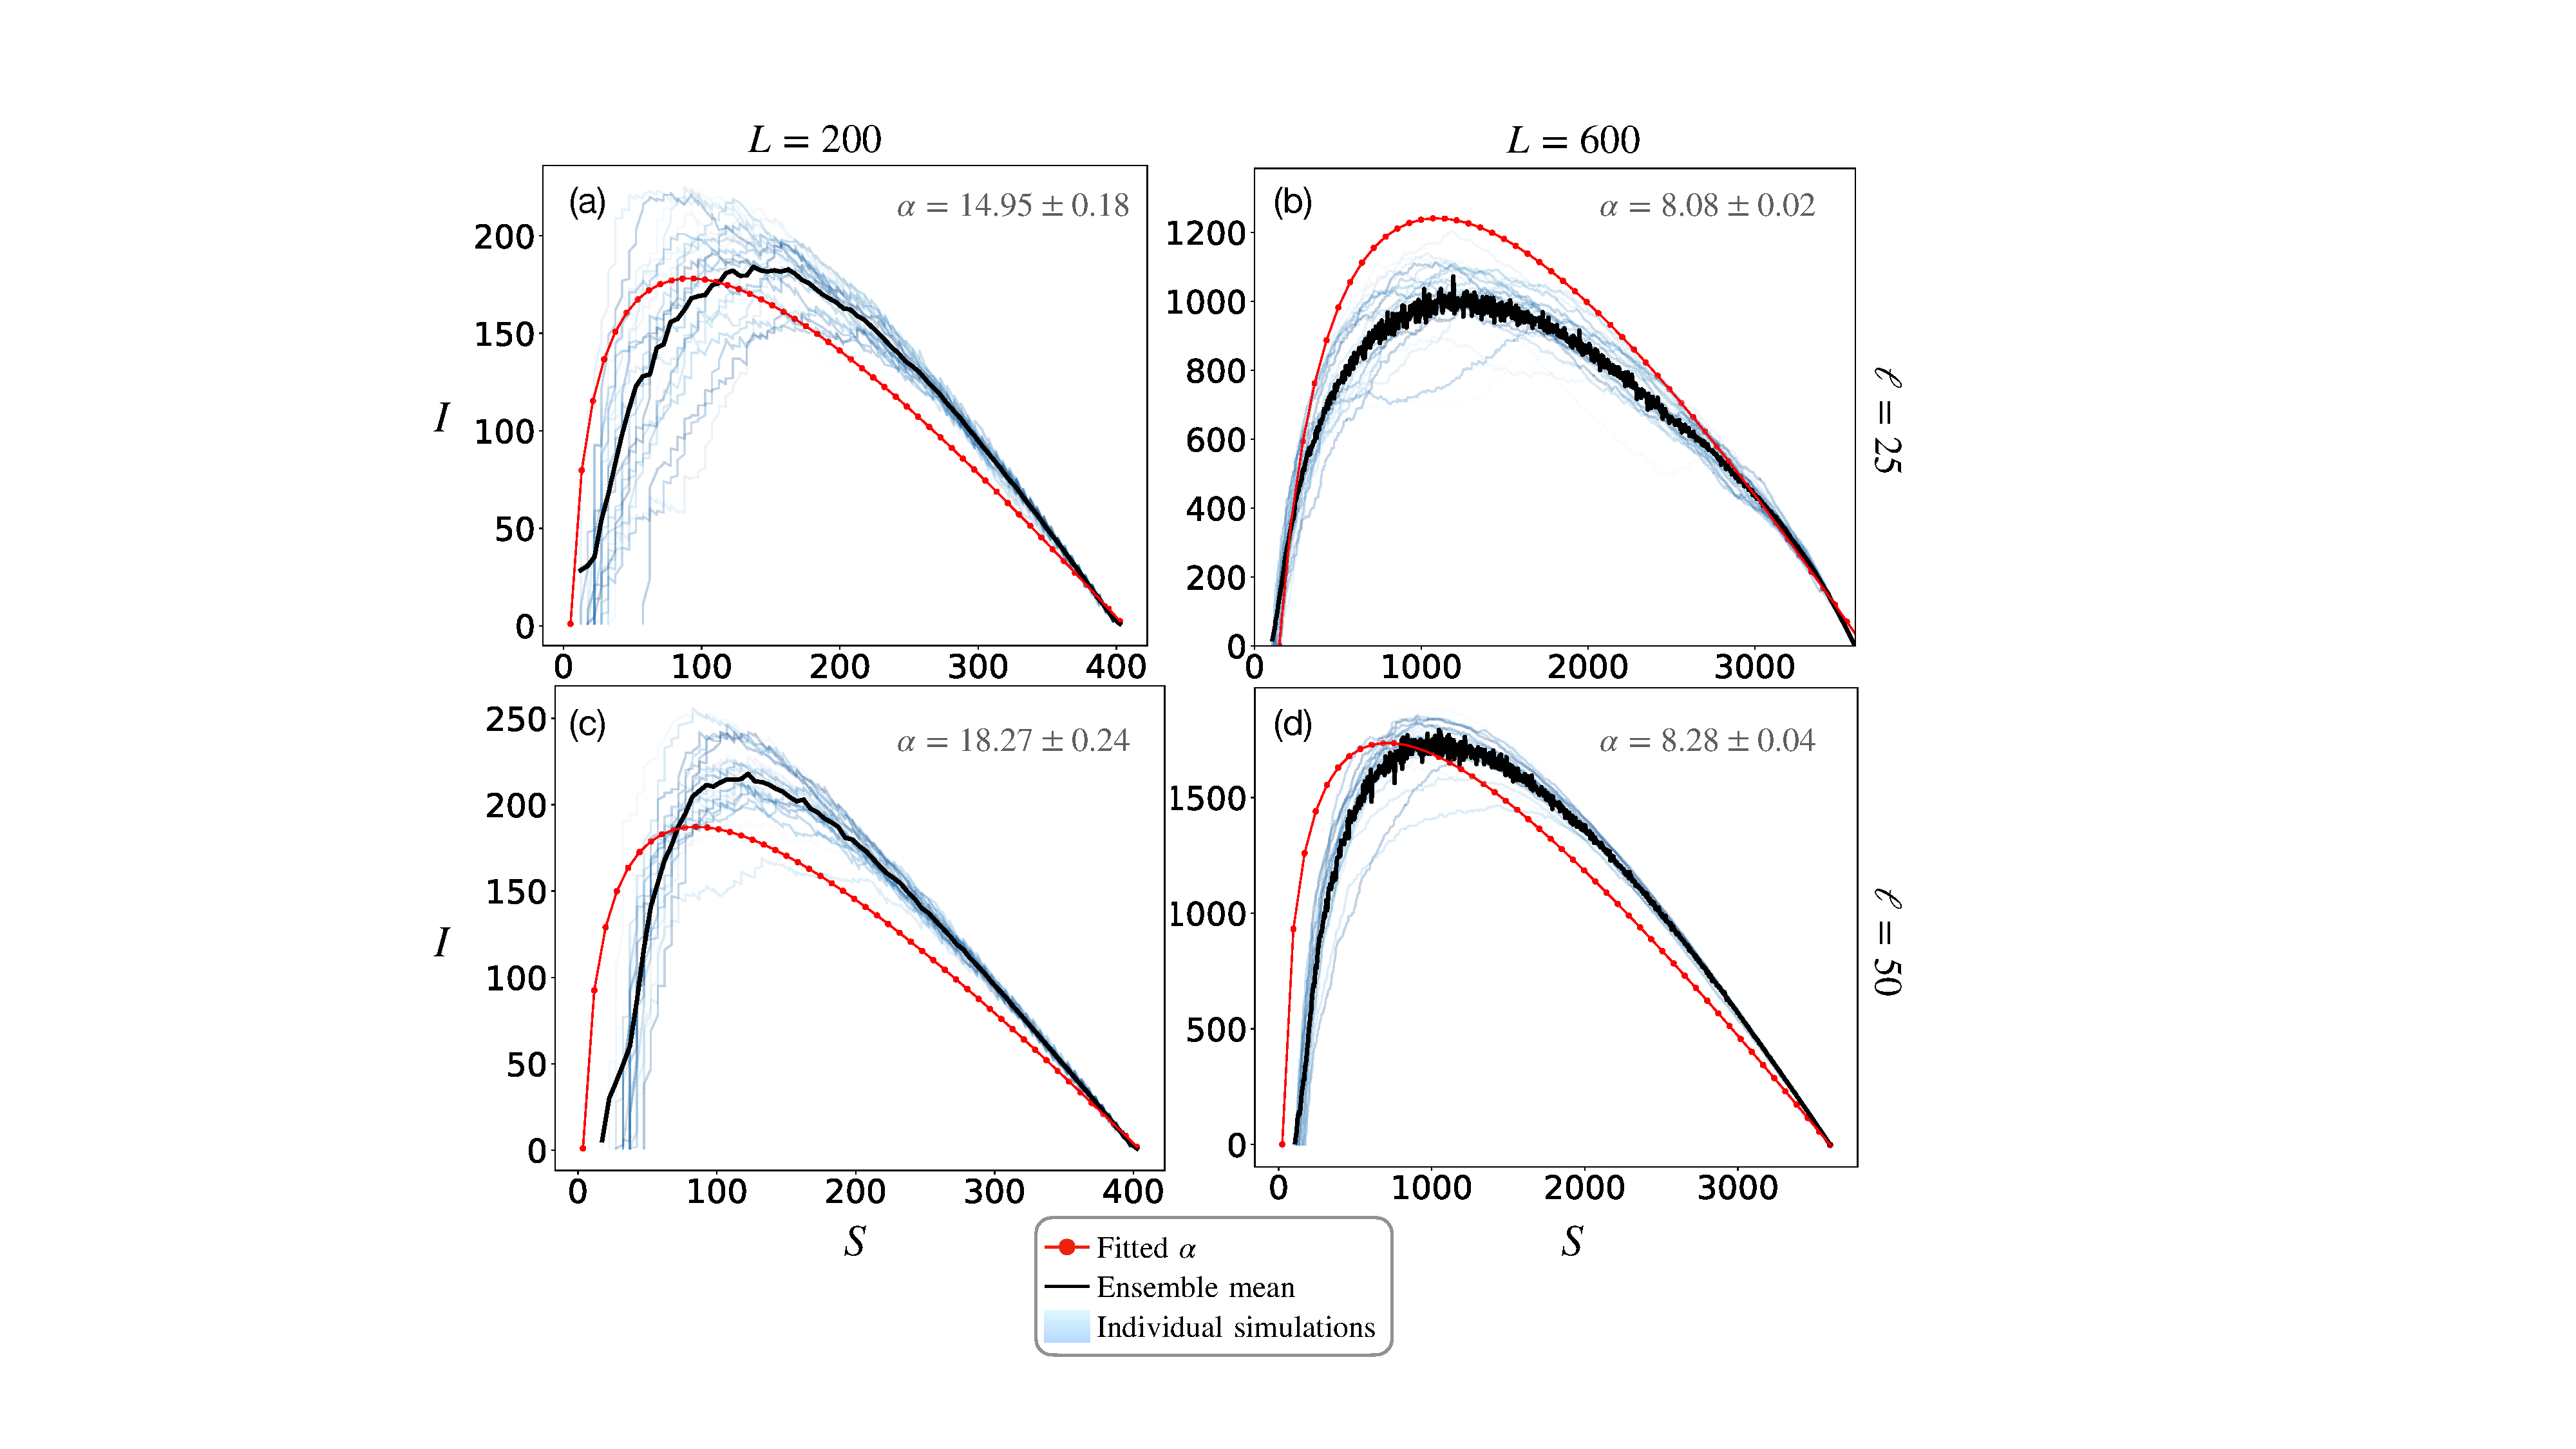
\includegraphics[scale=0.425]{chapter5/figures/fig2-sir-fitting-step.pdf}
    \caption{Fitting the non-local dispersal model (NLM) to the traditional SIR model given by \cite{kermack-model}. All simulations evolved with parameters $\beta^{*}=4$ and $\rho=0.01$ above the threshold for spread. (a) A small localised dispersal kernel of $\ell=25$ fitted against the canonical SIR. On a small domain of size $200\times 200$, the NLM spreads faster than the fitted SIR model. (b) On a larger patch of size $600\times 600$, the SIR model predicts a faster rate of spread in comparison to the NLM, illustrated by the disparity between red and black lines. (c) On $200\times 200$ sized domain, increasing the dispersal parameter to $\ell=50$ results in a similar trend to panel (b), albeit with slightly less agreement between NLM and SIR models. (d) Increasing the dispersal parameter to $\ell=50$ reduces the large disparity between SIR and NLM, shown in Figure (b).}
    \label{fig:SIR-fitting}
\end{figure}

Interestingly, for all but one panel in Figure \ref{fig:SIR-fitting}, epidemics progress faster in the NLM than predicted by the SIR model\textemdash indicated by the NLM having a steeper gradient beginning from $S_0=\rho\mathcal{L}^2$. 
One possible cause of disparity between models is due to infectious lifetime dynamics. 
Exponentially distributed lifetimes are implicit within the SIR model.
Whereas, the NLM relies on uniform transitions into the $R$ compartment that understood by examining Figure \ref{fig:SIR-fitting}(a), i.e. 400 hosts are present in the domain at time $t=0$ and it takes precisely $t=100$ steps to elapse before the first transition into $R$.

On the other hand, trees evolving with SIR dynamics will gradually transition into the $R$ compartment at all time steps according to an exponential distribution. 
For the same initial conditions, it follows that more infectious trees might be expected in the NLM between times $t\in [0, T]$, leading to more secondary infections that, on average, increase the scale of epidemic.
In appendix \ref{section:apendix_A}, Figure \ref{fig:SIR-fitting} is replicated, although equation \ref{eq:SIR-1param} was fitted to an exponentially distributed variant of the NLM.
Consequently, Figure \ref{fig:SIR-fitting-expontial} in appendix \ref{section:apendix_A} shows, a closer fit to equation \ref{eq:SIR-1param}.
 
Figure \ref{fig:SIR-fitting}(b) demonstrates another important aspect of NLM behaviour related to contact mixing in the spatial host distribution.
Looking at Figure \ref{fig:SIR-fitting}(b), a faster rate of spread is predicted for the SIR model,
demonstrated the divergence between red and black lines.
In this regime, $\frac{\ell}{\mathcal{L}}$ in the NLM is small, and contact-mixing in the host distribution can be assumed low \textemdash supported by Figure \ref{fig:sgm-evol} that demonstrated a wave-like spread. 
Moreover, the disparity between models is reduced by increasing the dispersal parameter to $\ell=50$, illustrated in Figure \ref{fig:SIR-fitting}(d).
Figure \ref{fig:SIR-fitting} therefore indicates that if the system is approximately well-mixed, the NLM spreads comparatively to the SIR, albeit slightly skewed because of uniform lifetime dynamics.
Whereas, if the system is not well-mixed, a slower epidemic marches across the domain in a wave-like manner that deviates significantly from the SIR model.
Altogether, these results point toward the inability of non-spatial models, such as the SIR model, to describe a spatially structured model of tree disease. That being said, in a parameter regime where the ratio $\ell / \mathcal{L}$ is sufficient for population mixing, the SIR model can describe the system with some accuracy\footnote{
Well-known results from percolation theory present a simple model analogy to the observations from Figure \ref{fig:SIR-fitting}.
Consider a large domain (of size $L$) below the percolation threshold, and sub-dividing the domain into boxes of size $\xi$, where $\xi / L$ is small.
Percolating clusters could be observed in each box i.e. at length scales comparable to $\xi$, but not $L$ see \cite{stauffer2018introduction} pages 64-65.}.


\section{A spatially-explicit reproduction number}
\label{sec:spatially-explicit-reproduction-ration}

As remarked earlier, percolation-based distance metrics become ill-defined when the pathogen can jump on long distances and a more robust metric is required to examine the model going forward.
As such, a basic reproduction number will be outlined for the NLM.
The concept of $R_0$ is widely used (and widely misinterpreted \cite{delamater2019complexity}),
and multiple methods of calculation exist in the literature \cite{perspectives-on-r0}.
Although, to recap, $R_0$ is fundamental to understand epidemic thresholds in human and animal populations. 

Crop-based reproduction ratios have been examined extensively
\cite{gubbins2000population, park2001invasion, doi:10.1146/annurev.phyto.011108.135838, van2011periodic},
yet the concept remains less explored in tree-based diseases. 
In general, $R_0$ is complicated, and may vary in response to numerous abiotic factors such as temperature, humidity and wind speed.
Notably, the threshold $R_0=1$ should separate regimes of epidemic and confinement for any definition of $R_0$.
Furthermore, when defining an $R_0$ value for tree-disease, the importance of spatial structure cannot be
ignored \cite{park2001invasion}.


\subsection{Approximating $R_0$ analytically}

In this section, an idealised, spatially explicit expression of $R_0$ is derived for the NLM. Defining an informative $R_0$-value for tree-based pathosystems is not simple, and care is needed when defining an $R_0$ value.  
The following thought experiment outlines an approach to approximate reproduction number:

\textit{Consider a single primary infected tree at time $t=0$, surrounded by a distribution of susceptible neighbouring trees. Throughout its infectious lifetime, the primary infection will lead to $R_0$ secondary infections. If secondary infections do not produce other tertiary infections, the neighbourhood around the primary infection remains untouched by other diseased trees, and the reproductive potential can be approximated by $R_0$.}

\begin{figure}
    \centering
    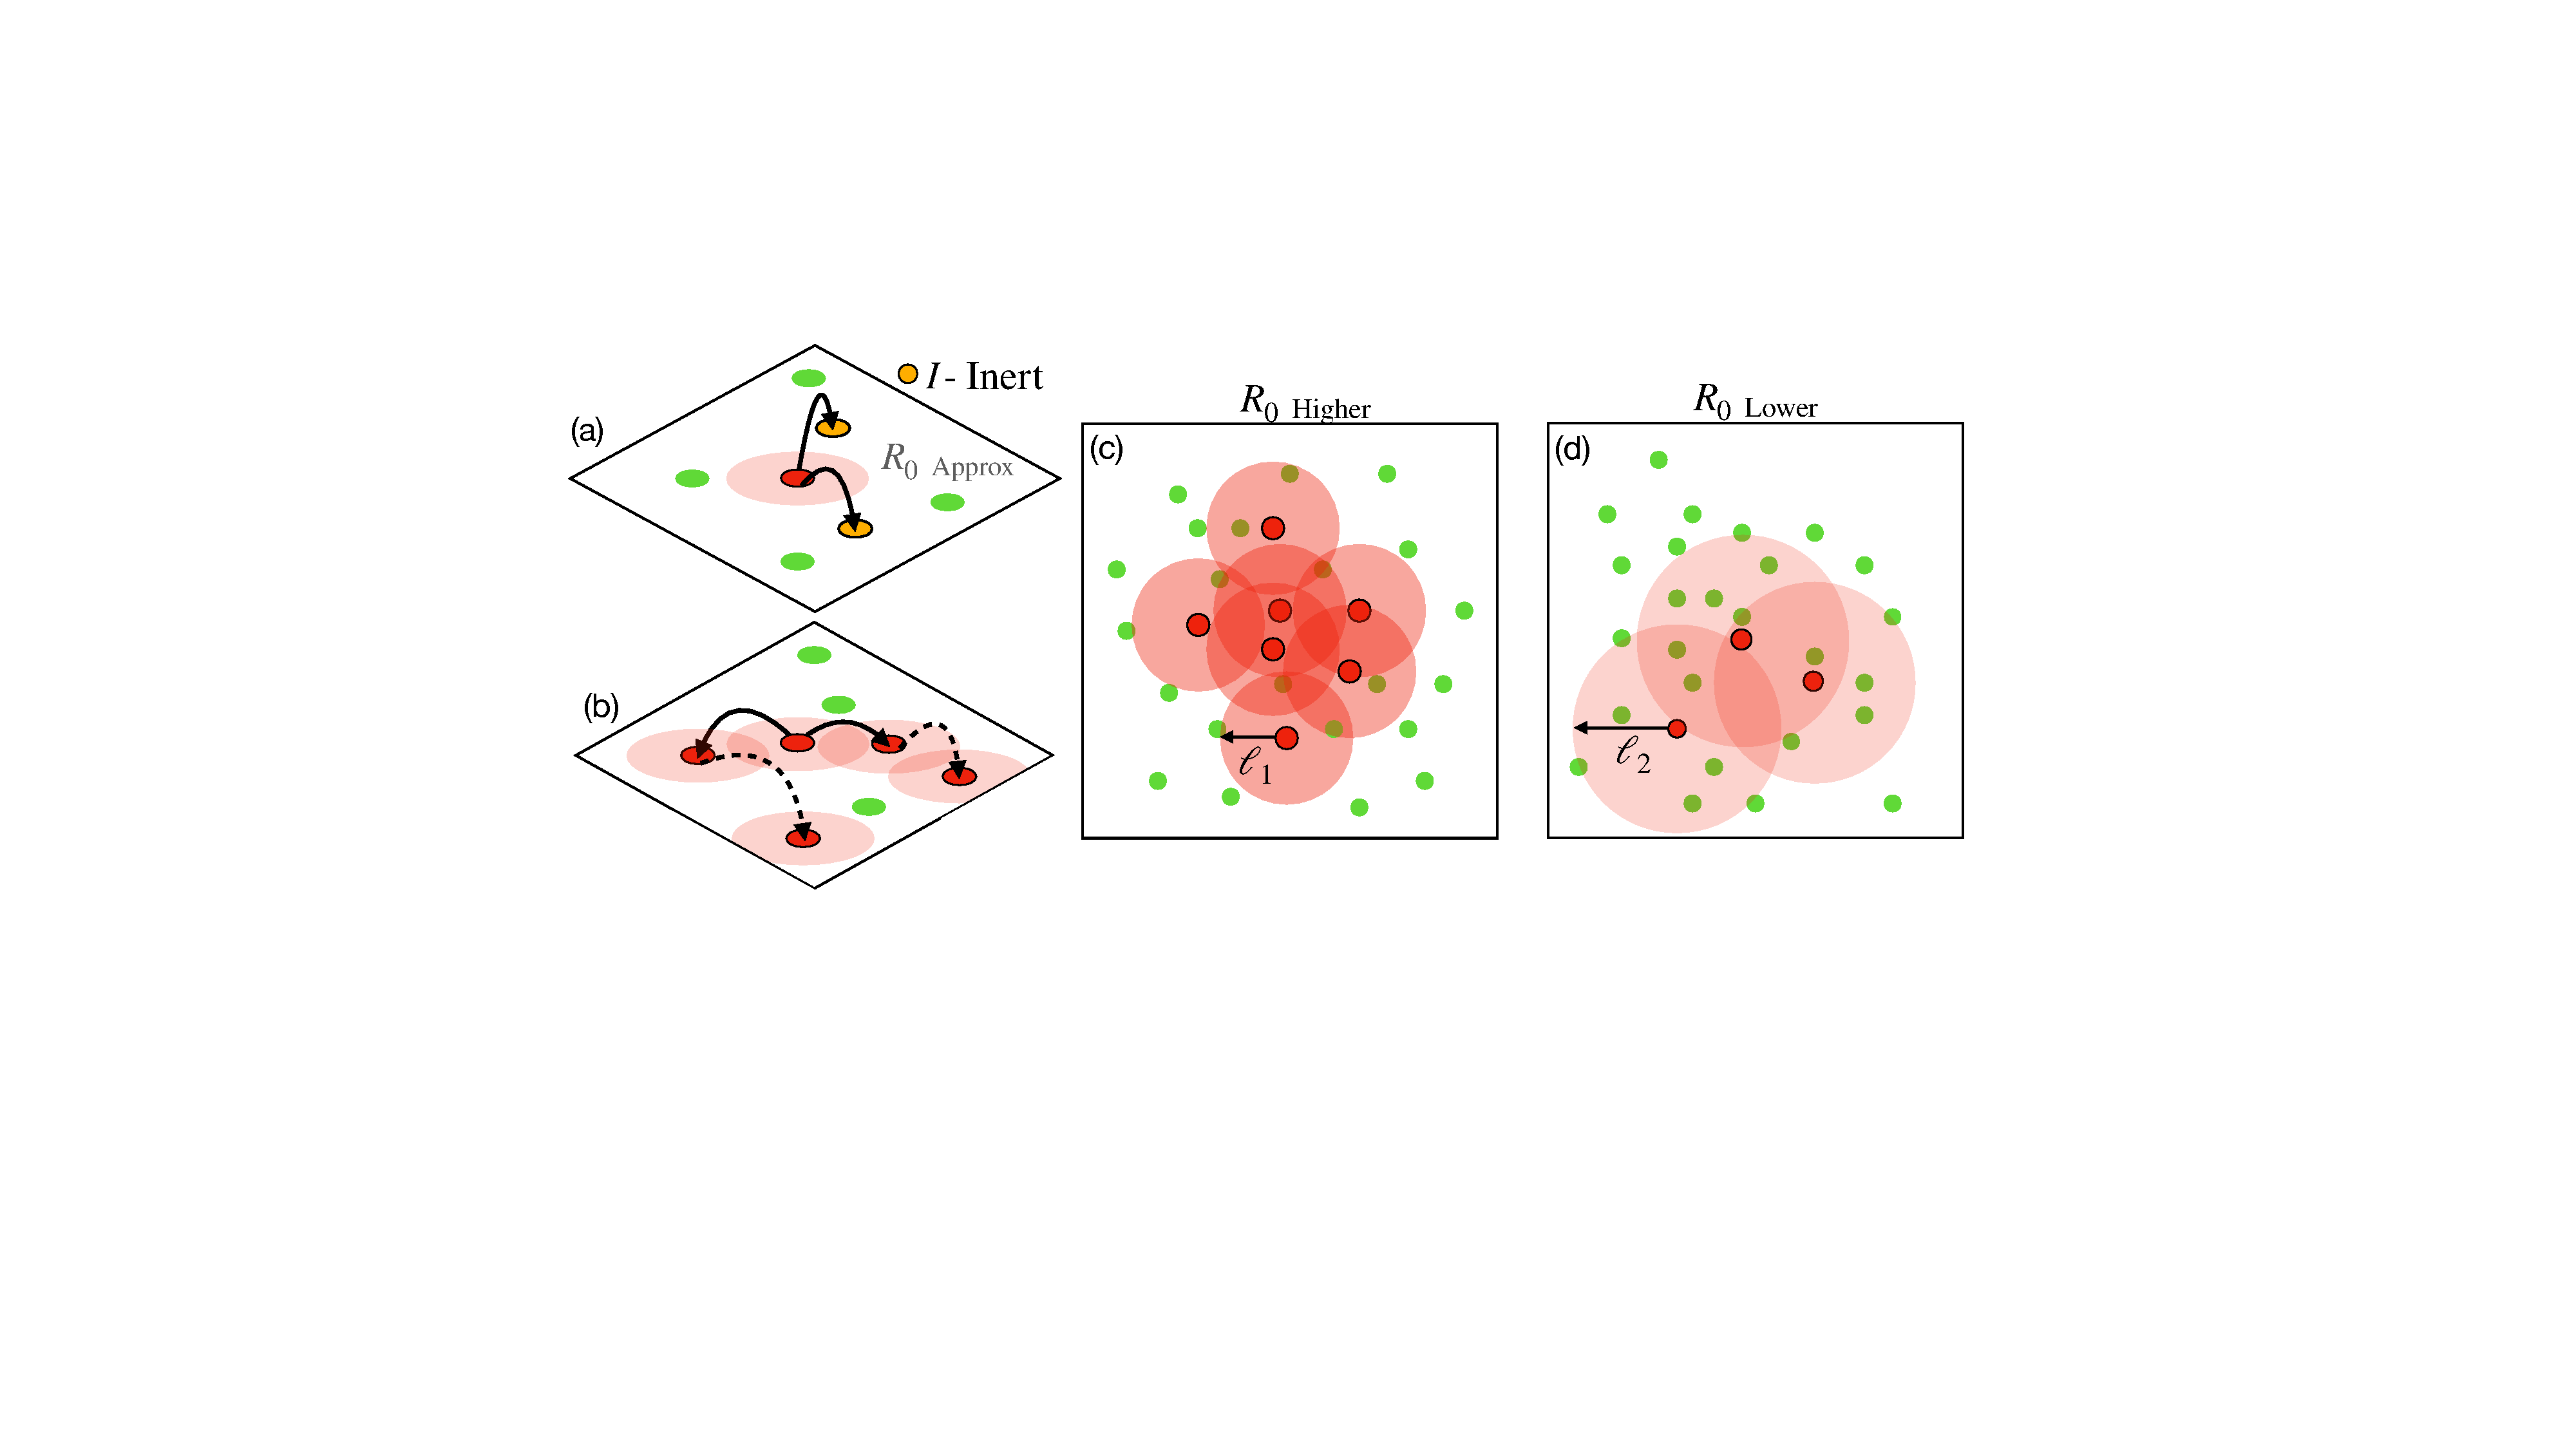
\includegraphics[scale=0.45]{chapter5/figures/fig3a-R0-approx.pdf}
    \caption{
    Approximating a spatially explicit value of $R_0$ as a function of $\rho$, $\beta$, $\ell$ and $T$.
    (a) An idealised scenario where secondary infections do not produce tertiary infections, but instead transition into an inert state\textemdash shown in amber.
    (b) The usual epidemic branching process where secondary infections produce tertiary (and so on) infections about the primary infection, shown by the solid and dashed arrows respectively.
    (c) Depictions of a highly infectious regime in the NLM, where $R_0$ is large and the dispersal parameter ($\ell_1$) is smaller.
    (d) Illustrations of an alternate, less invasive system when the scale of dispersal ($\ell_2$) happens to be larger. 
    The $R_0$ derivation aims to compute the scenario shown in (a), and becomes accurate in the epidemic regime illustrated in (d).
    }
    \label{fig:R0-approx}
\end{figure}

The thought experiment simplifies the epidemic branching process by neglecting tertiary (quaternary, and so on) infections,
illustrated by comparing Figures \ref{fig:R0-approx}(a-b). In turn, simplifying the system will help keep the mathematics tractable and permit an analytic derivation of $R_0$ without advanced mathematics. However, the derivation will be idealised and likely to overestimate the actual reproduction ratio in specific epidemic regimes.

Figures \ref{fig:R0-approx}(c-d) illustrate two hypothetical epidemic systems, with higher and lower $R_0$ values.
When the scale of dispersal is smaller (but still larger than the average distance between trees) and infectivity is high, as in Figure \ref{fig:R0-approx}(c), we expect a coupled system with a large number of secondary infectious induced inside a smaller area. In this case, the $R_0$ approximation would deviate from model simulations because secondary/tertiary infections would reduce the host density about the primary infection.
In other words, the finite-sized population gives rise to negative spatial correlations when other infected trees reduce the local density of susceptible hosts. The reader is referred to \cite{R0-perc-ref} for a helpful discussion of $R_0$, heterogeneity, spatial correlations and finite-size effects.

Conversely, Figure \ref{fig:R0-approx}(d) depicts a scenario when the pathogen induces a lower number of secondary infectious over a larger area. Hence, in the limit where secondary/tertiary infected trees do not influence the local density around the primary infection, the thought experiment (mentioned above) is expected to become increasingly accurate. 
However, even with a larger dispersal kernel, the approximation illustrated by Figure \ref{fig:R0-approx}(a) would become more inaccurate for highly invasive systems with a large $R_0$. 

For example, incredibly high values $R_0\in [30, 70]$ have been estimated for wheat stripe rust (WSR) epidemics \cite{severns2019consequences, mikaberidze2016invasiveness}. Nevertheless, 
a field of crops is significantly dense in comparison to an average tree population distributed over the landscape\textemdash discussed extensively in section \ref{sec:ch4-discussion} concerning oak. Consequently, we argue that, in general, the reproduction ratio of a tree pathogen is unlikely to reach super epidemic regimes that parallel WSR epidemics;
supported further by estimates of $1 \lessapprox R_0 \lessapprox 6$ for the Dutch elm disease epidemic in GB \cite{swinton1996dutch} and $1 \lessapprox R_0 \lessapprox 4$ for oak processionary moth epidemics in London [private correspondence with Dr Laura Wadkin, Newcastle University\footnote{Pre-prints of the publication can be found at https://www.biorxiv.org/content/10.1101/2021.12.09.471950v2} ].

\subsection{Derivation}

Suppose the domain is uniform with density $\rho_0$ at time $t=0$, and one singular infected tree exists inside a large domain.
In such a configuration, the mean number of secondary infections expected over the first time-step can be calculated by integrating equation \ref{eq:pr-dispersal-transition} as follows:
\begin{equation}
    R_0(t = 0) = \beta \rho_0 \int^{\infty}_{-\infty} \exp\Big(-\frac{r^2}{2\ell^2}\Big)dr= 2\pi\beta\rho_0\ell^2
\end{equation}
If host (re-)growth is neglected, less trees are available to infect at time-step $t+1$. 
Tree density can therefore be seen as a monotonically decreasing function of time $\rho(t)$, leading to the expression:
\begin{equation}
    R_0(t) = 2\pi\beta\ell^2\rho(t)
    \label{eq:r0-A}
\end{equation}
this expression presents a convenient relationship between tree density and the number of expected secondary infections. 
In a large but finite domain, of size $\mathcal{L}$, tree density approximately follows:
\begin{equation}
\label{eq:drho/dt}
    \frac{d\rho}{dt} = - \frac{R_0(t)}{\mathcal{L}^2} = -\frac{2\pi\beta\ell^2\rho(t)}{\mathcal{L}^2}
\end{equation}
Solving the above, with initial condition $\rho_0$ at $t=0$, leads to:
\begin{equation}
\label{eq:rho(t)-linear}
    \rho(t) = \rho_0 \exp\Big(-\frac{2\pi\beta\ell^2}{\mathcal{L}^2} t \Big)
\end{equation}
If density reductions from other secondary and tertiary infections are neglected, the final number of expected secondary infections after $T$ infectious time-steps is given by:
\begin{equation}
\label{eq:Appendix_final_r0_approx}
    R_0(T) =  \mathcal{L}^2\big(\rho_0 - \rho(T)\big) = \mathcal{L}^2\rho_0\Big[1 - \exp\big(-\frac{2\pi\beta\ell^2}{\mathcal{L}^2} T \big) \Big]
\end{equation}
Equation \ref{eq:Appendix_final_r0_approx} can be used as a first approximation toward an $R_0$ value\textemdash the reader can find an equivalent, discrete-time derivation in Appendix \ref{eq:alternate-R0}.
Nonetheless, uniform density reductions (in equation \ref{eq:drho/dt}) assume that secondary infections are equally likely at all spatial locations about the primarily infected tree. 
On average, neglecting spatial variations overestimates the number of secondary infections induced by the tail-ends of the dispersal kernel,
thus giving rise to a greater $R_0$ value.
A more accurate, albeit more complex, equation can be derived, allowing for Gaussian spatial variations

For transparency, the above derivation is solely based on $\beta$, and not the normalised infectivity parameter. 
However, from the exponential exponent in equation \ref{eq:Appendix_final_r0_approx}, it is clear to see how normalising the infectivity ($\beta^*/2\pi\ell^2$) prevents
the number of expected secondary infections dependency on $\ell$. That is, substituting $\beta^*/2\pi\ell^2$ into the equation \ref{eq:Appendix_final_r0_approx} leads to an exponent, (i.e. $T\beta^*/L^2$) independent of $\ell$.

\subsubsection{Incorporating Gaussian dispersal}

\label{sec:r0-derivation}
Equation \ref{eq:Appendix_final_r0_approx} neglects a spatially varying transmission probability, 
though it can be refactored by first re-writing the density as:
\begin{equation}
\label{eq:rho(t)-ga-variations}
    \rho(r, T) = \rho_0\exp \big(-\beta T g(r; \ell) \big)
\end{equation}
where $g(r;\ell)$ is a Gaussian kernel. 
Equation \ref{eq:rho(t)-ga-variations} can be interpreted as the generalised form of equation \ref{eq:rho(t)-linear}, this time incorporating Gaussian spatial variations into $R_0$.
Upon substitution back into equation (\ref{eq:Appendix_final_r0_approx}), the total number of secondary infections after $T$ time-steps is given by:

\begin{equation}
\label{eq;R0(t)-ga-variations}
   R_0(T) = \int ^\infty _0 2\pi r \big (\rho_0 - \rho(r, T)\big)dr =  \int ^\infty _0 2\pi r \rho_0 \Big[1 - \exp\big(-\beta T g(r;\ell)\big) \Big]dr
\end{equation}

Note, the finite lattice square of size $\mathcal{L}^2$ has been replaced with integration in polar coordinates over $dr$. 
Equation \ref{eq;R0(t)-ga-variations} is hard to solve directly, but it can be integrated by performing a series expansion on the exponential term. 
One may then proceed to integrate on a term-by-term basis:

\begin{equation} 
\label{eq:Appendix_final_expression}
\begin{split}
R_0(T) & = \int^\infty_0 2\pi r \rho_0 \Big[1 - \exp \big( -\beta T g(r;\ell)\big)\Big]dr \\
& = 2\pi\rho_0 \int^\infty _0 r \Big[1 - \sum^\infty_{n=0} \frac{\big(-\beta T)^n}{n!} \exp\big(-\frac{r^2}{2\ell^2}\big)^n  \Big] dr \\
& = 2\pi\rho_0 \int^\infty _0 r \Big[\sum^\infty_{n=1} \frac{(-1)^{n+1}\big(\beta T)^n}{n!} \Big(\exp(-\frac{n r^2}{2\ell^2} ) \Big)  \Big] dr \\
& = 2\pi\rho_0 \sum^{\infty}_{n=1} \frac{(-1)^{n+1} (\beta T)^n}{n!} \int^\infty _0 r \exp(-\frac{n r^2}{2\ell^2})dr  \\
& = 2\pi\rho_0 \ell^2 \sum^{\infty}_{n=1} \frac{(-1)^{n+1}(\beta T)^n}{(n)(n!) }
\end{split}
\end{equation}

if $\beta$ and $T$ are small, the $1^{st}$ order term in equation \ref{eq:Appendix_final_expression} is sufficient to approximate $R_0$ as a linear function of $T$\textemdash
confirmed by numerical simulations in the next section. 
Finally, equation \ref{eq:Appendix_final_expression} can be summed to give:
\begin{equation} 
\label{eq:Appendix_final_expression1}
\begin{split}
R_0(T) & = 2\pi\rho_0 \ell^2 \sum^{\infty}_{n=1} \frac{(-1)^{n+1} (\beta T)^n}{(n)(n!)}\\
& =  2\pi\rho_0 \ell^2 \big(E_1(\beta T) + \ln (\beta T) + \gamma\big)
\end{split}
\end{equation}
where the function $E_1(x)$ is the mathematically well studied exponential function $E_1(x)=\int^{\infty}_x t^{-1}\exp^{-t}dt$ and $\gamma$ is the Euler–Mascheroni constant $\approx 0.57721$.
Intriguingly, the jump between equations \ref{eq:Appendix_final_expression} and \ref{eq:Appendix_final_expression1} is well known in the field of complex analysis\textemdash see \cite{abramowitz1948handbook}, page 228.
Alternatively, the summation in equation \ref{eq:Appendix_final_expression} could equivalently be given as:
\begin{equation}
\label{eq:ein}
     \mathrm{Ein}(\beta T) = \sum^{\infty}_{n=1} \frac{(-1)^{n+1} (\beta T)^n}{(n)(n!)}
\end{equation}
where $\mathrm{Ein}$ is known as the `entire' function, leading to the well established relation:
\[
E_1(z) = -\gamma - \ln(z) + \mathrm{Ein}(z)
\]
The next section will investigate the suitability of \ref{eq:Appendix_final_expression1} to describe the NLM.

\section{$R_0$ behaviour: analytics vs numerics}

% R0 can be calculated from experimental data : \cite{segarra2001epidemic}
% \label{ch5:dispersal-model}
\begin{figure}
    \centering
    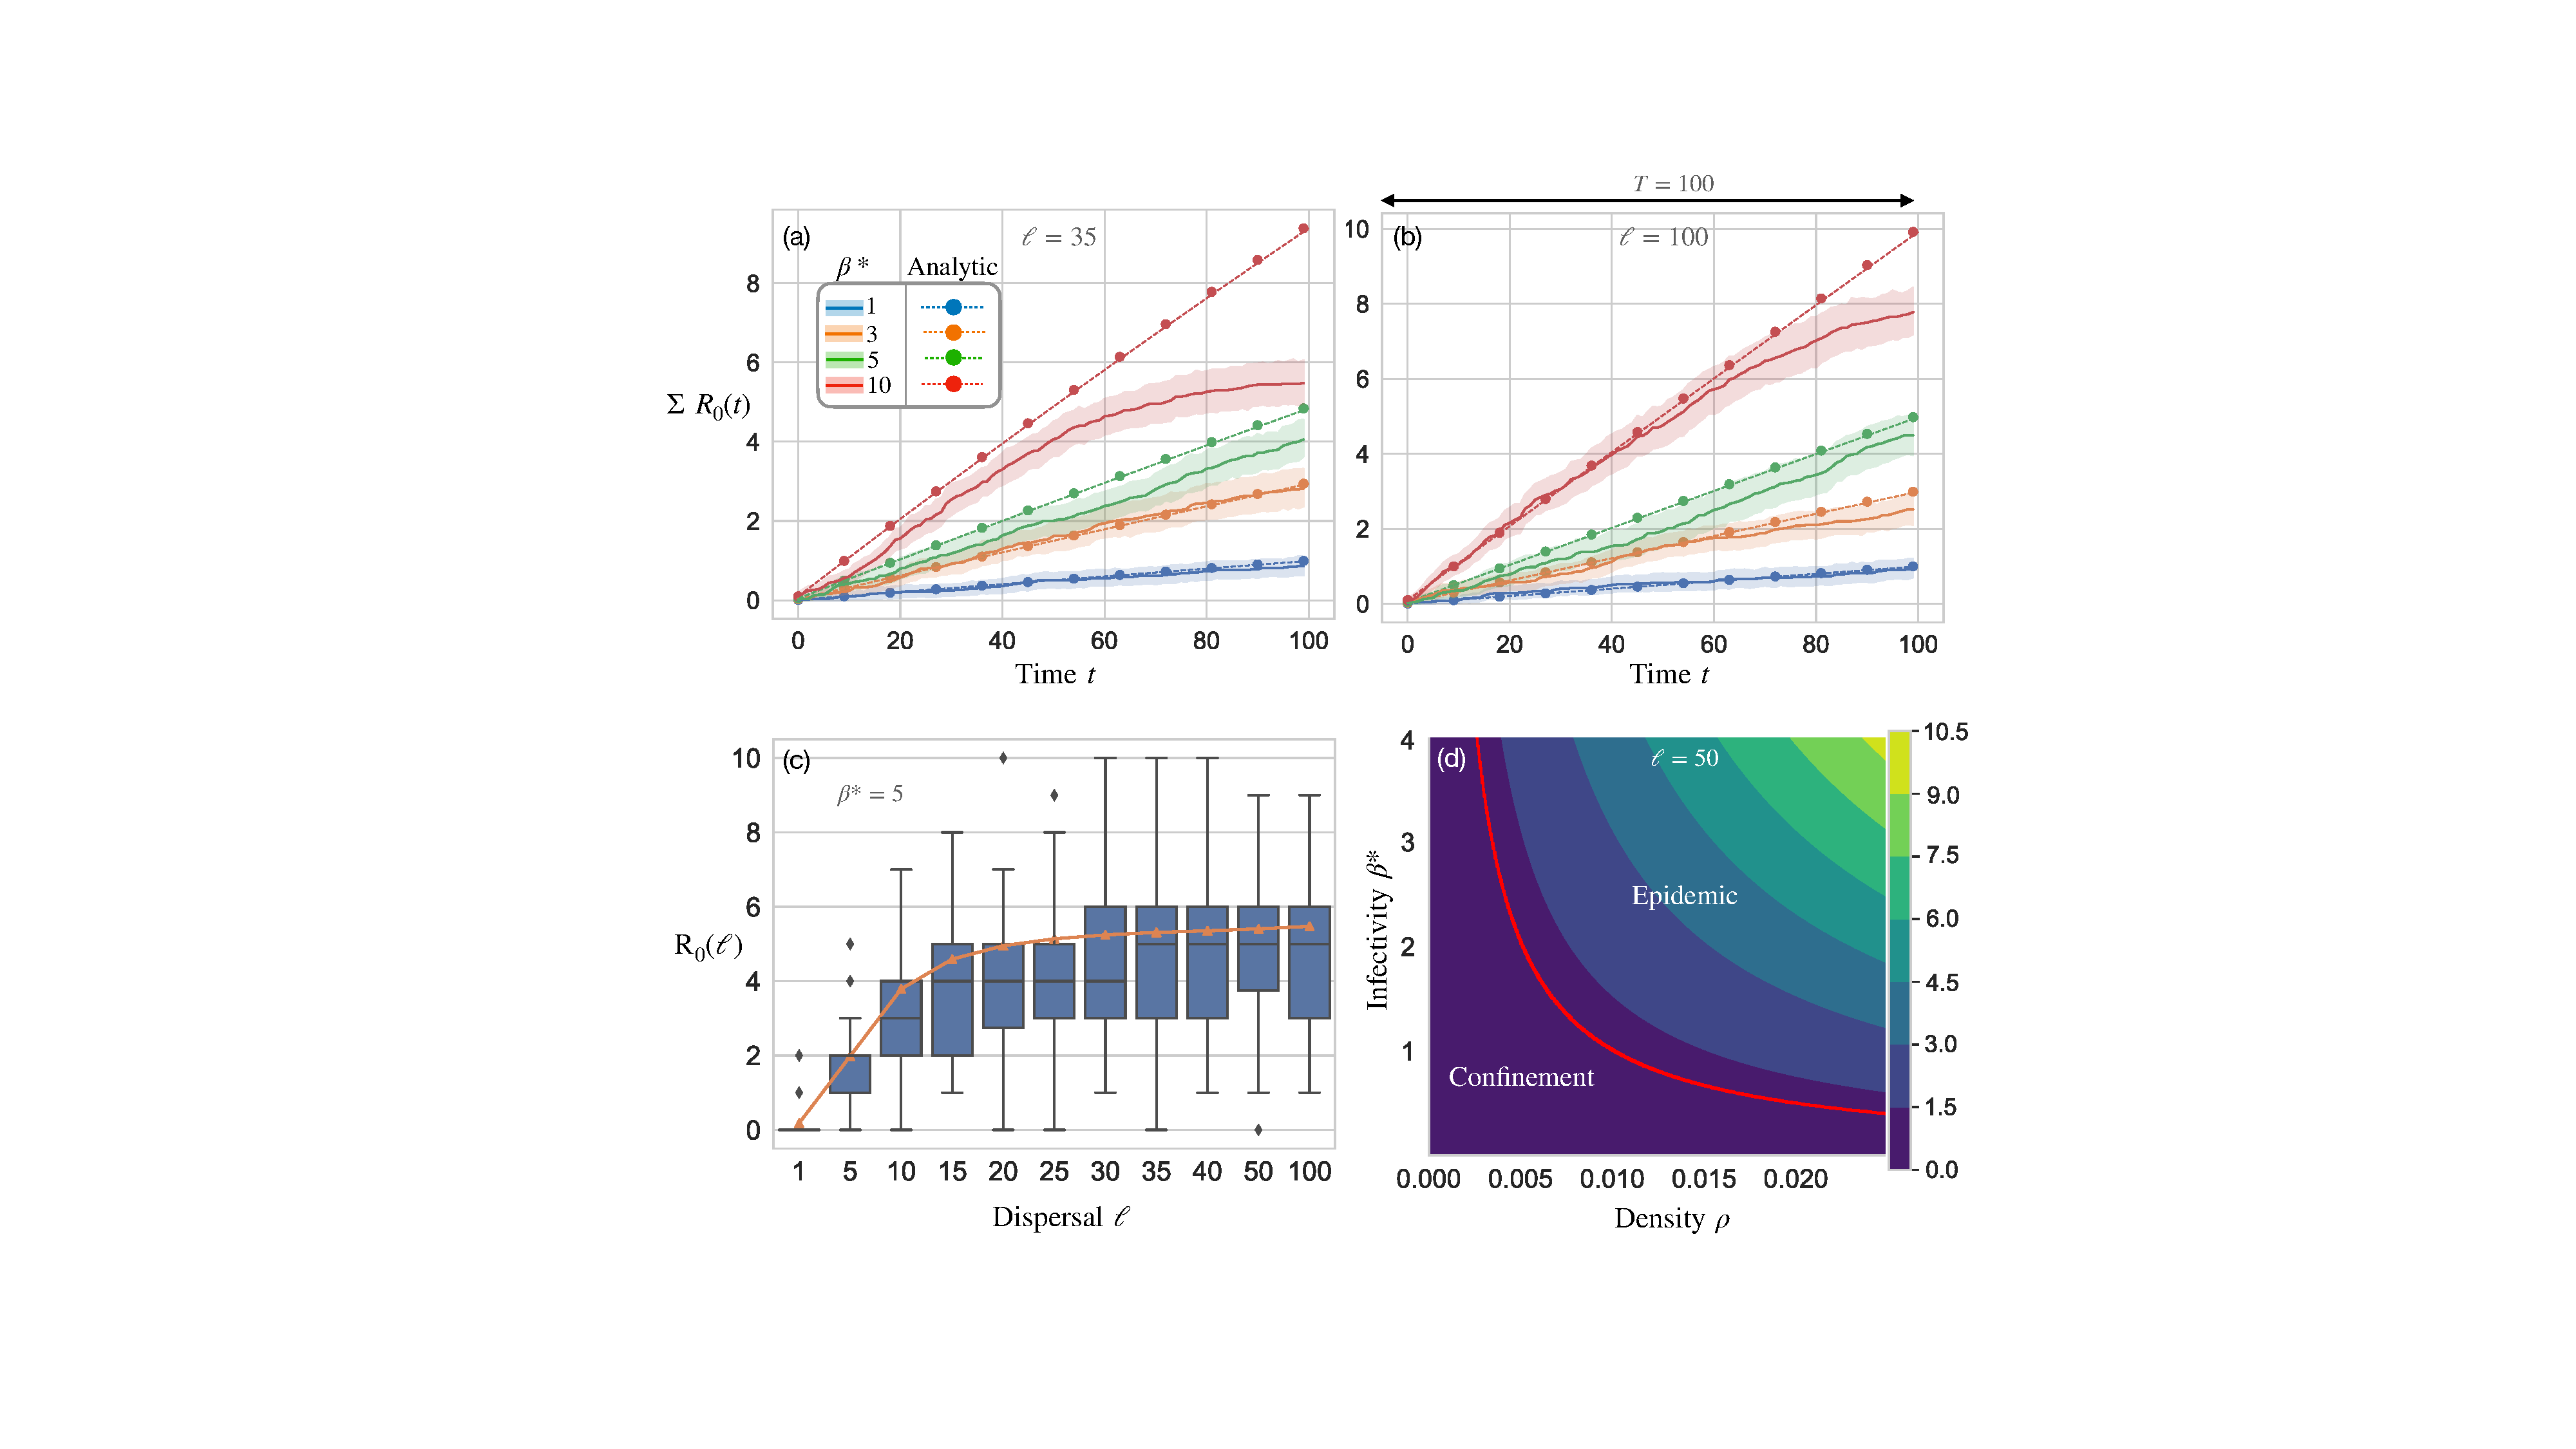
\includegraphics[scale=0.475]{chapter5/figures/fig3b-R0-analytic.pdf}
    \caption{Comparisons between the analytical expression for $R_0$, according to equation \ref{eq:Appendix_final_expression1}, and numerical simulations.
    In panels (a-b), The cumulative sum of secondary infections are ensemble-averaged (50 repeats) over the infectious lifetime of $T=100$ steps.
    (a) When the scale of dispersal is smaller ($\ell=35$), a high infectivity (in red) causes $R_0$ to saturate to a maximum over the infectious period.
    For smaller infectivities (blue-green), $R_0$ increases at a constant rate and fails to saturate.
    (b) For a larger dispersal kernel ($\ell=100$) and high infectivity, $R_0$ increases at a more constant rate, 
    yet deviations still exist at the conclusion of its infectious lifetime.
    (c) $R_0$ is shown as a function of the dispersal parameter for fixed infectivity $\beta^*=5$. For small length scales, the normalised infectivity produces a less infectious outbreak. However, $R_0$ is approximately fixed for larger $\ell$ values. Analytic predictions, shown in orange, tend to overestimate the spread for small $\ell$.
    (d) The 2D $R_0$ phase plane predicted by equation \ref{eq:Appendix_final_expression1}. A threshold, given by $R_0=1$, is plotted in red that predicts the separation between confinement and epidemic.}
    \label{fig:R0-analytic-vs-sims}
\end{figure}

In Figure \ref{fig:R0-analytic-vs-sims}, the analytic predictions of $R_0$ from equation \ref{eq:Appendix_final_expression1} are compared against numerical simulations. 
Figures \ref{fig:R0-analytic-vs-sims}(a-b) plot the total number of secondary infections due to the primary infection over its lifetime, denoted by $\sum_{t=0}^T R_0(t)$.
In both panels (a-b), NLM simulations were ensemble-averaged $N=50$ times for four infectivity values, indicated by the solid coloured lines. 
The final value of $R_0$ is observed when the infectious lifetime of $T=100$ steps is concluded.
Figures \ref{fig:R0-analytic-vs-sims}(a-b) show two epidemic scenarios, with lower ($\ell=35$) and higher ($\ell=100$) dispersal parameters.
As expected, equation \ref{eq:Appendix_final_expression1} tends to overestimate $R_0$ for both dispersal parameters when infectivity is high, illustrated by the dotted scatter plot.

The time-series in Figure \ref{fig:R0-vs-NLM-sims}(a) reveals that lower $\beta^*$ parameters produce a constant infection rate, indicated by linear relationship in blue-green.
Equation \ref{eq:Appendix_final_expression1} agrees well with these lower infectivity parameters. However, large deviations from model output can be seen for $\beta^*=10$ at later times. 
Here, the number of new secondary infections plateau for $\beta^*=10$ because other secondary/tertiary infections reduce host density around the primary infection. Subsequently, at later times, fewer and fewer trees in the primary infections neighbourhood are available to infect, causing $R_0$ to level off.
Thus, equation \ref{eq:Appendix_final_expression1} describes constant transition rates accurately but deviates from model simulations when infection rates decrease because other (secondary/tertiary) infections reduce host local densities.

In Figure \ref{fig:R0-vs-NLM-sims}(b), the dispersal parameter is increased to $\ell=100$.
A larger dispersal kernel encompasses a larger neighbourhood.
Subsequently, $R_0(t)$ saturates less for higher $R_0$ values, in contrast to Figure \ref{fig:R0-vs-NLM-sims}(a).
Despite a surprising degree of simplicity, the linear relation for lower $\beta^*$ parameters is predicted by equation \ref{eq:Appendix_final_expression1}.
The linearity can be understood by noting that when $\mathrm{Ein}(\beta T)$ is small in comparison to $\ell^2$ (and $\beta T$ is small), the first-order term inside equation \ref{eq:Appendix_final_expression1} reduces to a linear equation in $T$.
More interestingly, however, we can observe that $R_0$ is similar when $\beta^*$ is low, revealed by comparing the blue-green lines in Figures \ref{fig:R0-vs-NLM-sims}(a-b).
Whereas, for higher infectivities, $R_0$ tends toward a smaller value in Figure \ref{fig:R0-vs-NLM-sims}(a) comparison to panel (b).
Observing $R_0$ deviate with different $\ell$ parameters compels a study of $R_0$ over the space of $\ell$, which leads to Figure \ref{fig:R0-vs-NLM-sims}(c).

In Figure \ref{fig:R0-vs-NLM-sims}(c), the basic reproduction number $R_0$ is assessed over a range of dispersal kernels.
Tree density in Figure \ref{fig:R0-vs-NLM-sims}(c) is fixed fixed to $\rho=0.01$ together with infectivity $\beta^*=5$.
Predictions from equation \ref{eq:Appendix_final_expression1} are shown in orange,
and $R_0$ can be seen to increase with the dispersal kernel up to around $\ell \in [25, 30]$ before saturating to $R_0 \sim 5$. 
When $\ell$ is small, $R_0$ is low; the reason for this are two-fold: 
(A) neighbourhoods defined by a small $\ell$ parameter are likely to become fully occupied by secondary-infected trees
(B) the scale of dispersal is less than the average distance between trees, thereby preventing the spread.
Then, as the kernel is increased, $R_0$ asymptotically increases to a maximum value beyond which increasing $\ell$ bares no impact on $R_0$\textemdash provided that the number of secondarily infected trees is small in comparison to the number of hosts in the neighbourhood\footnote{Insight into the underlying behaviour could be gleaned by looking at equation \ref{eq:Appendix_final_expression1}. That is, by accessing the growth of $2\pi \rho_0 \ell^2$ and the convergence of the function $\mathrm{Ein}$ (defined by equation \ref{eq:ein}) and noting that as $\ell \rightarrow \infty$, $\beta=\beta^*/2\pi\ell^2 \rightarrow 0$. Although an in-depth mathematical analysis was not undertaken, it is clear that for large values of $\ell$, $R_0$ asymptotically approaches a limiting value.}.
Therefore, if $\ell$ is large enough, the normalised infectivity can be seen to effectively constrains the epidemic severity to a limiting value.

From the reproduction number, a transmission threshold can be defined by $R_0=1$,  predicting the separation of states between confinement and epidemic.
In Figure \ref{fig:R0-vs-NLM-sims}(d), the threshold predicted by equation \ref{eq:Appendix_final_expression1} is marked in red, overlaying a two-dimensional phase plot of $R_0$ over tree density and infectivity.
According to Figure \ref{fig:R0-vs-NLM-sims}(d), when model parameters satisfy $R_0>1$, the pathogen may propagate for a time before dying off or culminate in an epidemic.
Below the threshold, the pathogen has little chance of spreading to neighbouring trees and little chance of causing a large-scale epidemic.
Equation \ref{eq:Appendix_final_expression1} provides a computationally efficient means to categorise model behaviour.
The following section assesses how the total tree mortality, or final-sized epidemic, relates to threshold $R_0>1$  predicted by \ref{eq:Appendix_final_expression1}.

\subsection{Tree mortality versus $R_0$}
\label{sec:tree-mortality-analytic}

Desirably, predictions about the final epidemic outcome should be possible given observations of the first few infections. 
For a well-mixed homogeneous population, the reproduction number can be used to estimate the number of expected cases as a fraction of the population.
In the standard SIR model, this is given by:
\begin{equation}
\label{eq:final-sized-epi}
    R_{\infty} = S_0\Big[]1 - \exp\big( R_0 R_\infty\big) \Big]
\end{equation}
where $R_\infty$ is the number of cases as a fraction of the population size (the so-called `final-sized epidemic'). 
When there is spatial structure, as in the NLM, the relation given by equation \ref{eq:final-sized-epi} would no doubt be more complex.
This section investigates the relationship between $R_0$ and the number of host removals during a simulation\textemdash compelled by the fact that multiple methods can calculate $R_0$ and that methods should be evidenced by the existence of a threshold \cite{li2011failure}.

Varying both $\rho$ and $\beta^*$ results in a different $R_0$ prediction.
In this way, $R_0$ predictions can be plotted against the total number of hosts transitioning into the $R$ compartment\textemdash labelled as `tree mortality' in Chapter\ref{fig:ch4_uk_spread}.
In Figure \ref{fig:R0-vs-NLM-sims}(a), ensemble-averaged tree mortalities are plotted as a function of the predicted $R_0$ value for three variations of tree density $\rho$, indicated by the solid blue-green lines.
Simulations were repeated in an ensemble of size $250$, and each simulation evolved until all infected trees became extinct or for $2500$ time-steps elapsed, whichever occurred first.
The ensemble-averaged mortality is overlaid by a scatter plot depicting a small sample of data points; the colour of each sample point reflects the infectivity parameter $\beta^*$.

\begin{figure}
    \centering
    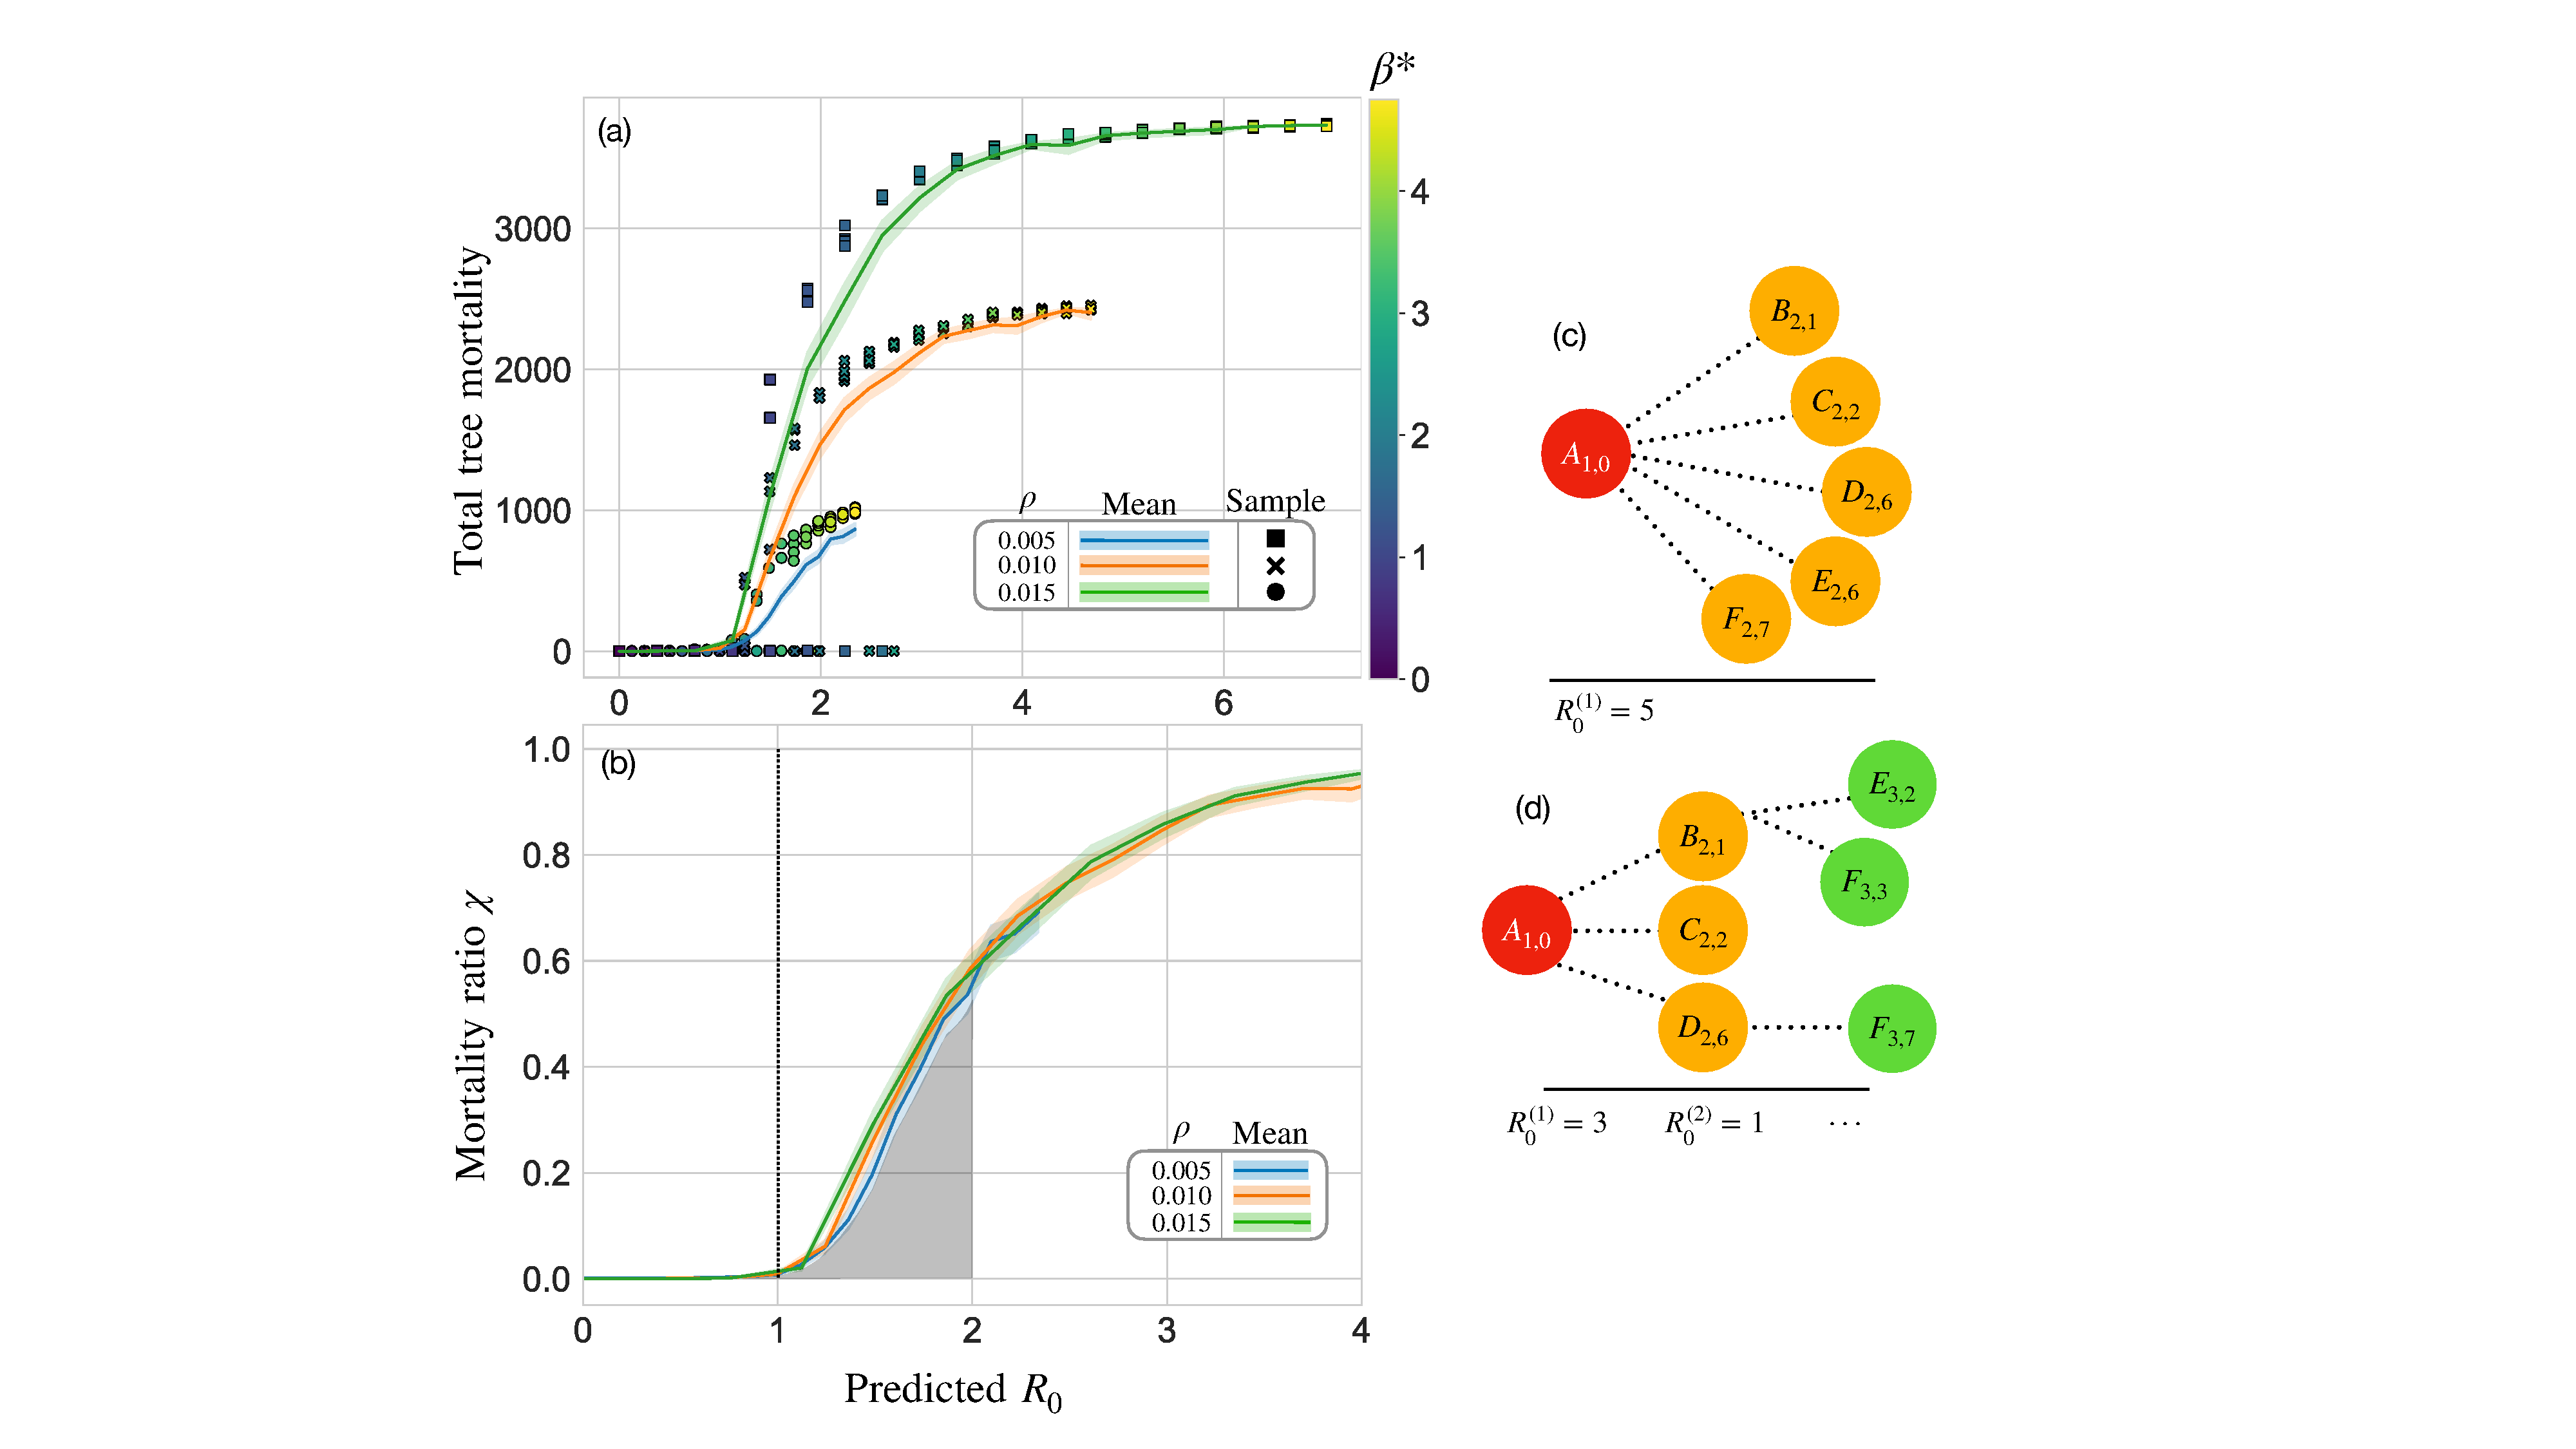
\includegraphics[scale=0.44]{chapter5/figures/fig4-R0-analytic-vs-mortality.pdf}
    \caption{The relationship between the total tree mortality and the predicted $R_0$ value. (a) For three values of tree density and multiple infectivity values, the ensemble-averaged tree mortality (as a continuous solid line) is overlaid with a small sample of data points shown by the scatter plot. The shape and colour of each data point indicate the tree density and infectivity, respectively. (b) The fraction of removed trees as a fraction of the population is plotted against mortality the analytical value of $R_0$. Together panels (a) and (b) demonstrate a threshold-like behaviour at $R_0=1$. (c) A graphical representation of the idealised $R_0$ approximation, as per equation \ref{eq:Appendix_final_expression1}. (d) A more realistic network representing the epidemic branching process. In both panels, the arrow of time is left to right, and subscripts reflect the generation and time-step that trees become infected.}
    \label{fig:R0-vs-NLM-sims}
\end{figure}

According to Figure \ref{fig:R0-vs-NLM-sims}(a), when $\beta^*$ is low the reproduction ratio satisfies $R_0<1$ and tree mortality is kept low.
Additionally, when the infectivity is increased such that $R_0>1$,  tree mortality rises considerably.
Equation \ref{eq:Appendix_final_expression1} therefore demonstrates a threshold-like behaviour defined by $R_0=1$.
Above the threshold $R_0=1$, increasing the tree density increases the epidemic scale because more susceptible hosts are available to infected\textemdash indicated by a more significant rise in tree mortality in green.

Despite being above the threshold, the numerical simulations can still fail to produce an epidemic,
illustrated by the small number of data points beyond $R_0=1$ that map to a zero-sized epidemic. For example, at $R_0\approx 2$ a small number of points can far below each ensemble mean.
Similarly, the ensemble mean is lowered by pathogen extinction\textemdash demonstrated by slight differences between the collection of points and the ensemble mean in the interval $R_0 \in [1, 3]$.
These observations result from the fact that under the influence of early stochastic forces, the probability of epidemic extinction is higher \cite{perspectives-on-r0, R0-perc-ref}, which unfortunately marks a flaw in the concept of $R_0$ in general \cite{li2011failure}.

Figure \ref{fig:R0-vs-NLM-sims}(b) presents the same essential information as Figure \ref{fig:R0-vs-NLM-sims}(a).
Although, the ensemble mean is plotted against the mortality ratio (i.e. the total number of removed trees as a fraction of the total population), denoted by $\chi$.
Given that each ensemble mean converges to the same epidemic scale, the quantity $\chi$ demonstrates utility when accessing the epidemic impact between different tree-densities.
Consequently, the threshold $R_0=1$ is easily observable in Figure \ref{fig:R0-vs-NLM-sims}(b), indicated in shaded grey.
The threshold-like behaviour witnessed in Figures \ref{fig:R0-vs-NLM-sims}(a-b) demonstrate that equation \ref{eq:Appendix_final_expression1} provides a simple predictive framework for the  NLM.
That said, more complicated dynamics\textemdash such as exponential lifetimes, elaborate dispersal kernels or host aggregation\textemdash could significantly hinder the analytic solution proposed in section \ref{sec:r0-derivation}.

Another limitation to the equation \ref{eq:Appendix_final_expression1} can be explained by Figure \ref{fig:R0-vs-NLM-sims}(c), which shows a typical NLM simulation used to access the analytic expression of $R_0$.
Namely, a single `fist-generation' infected tree at time $t=0$ ($A_{1, 0}$) that happens to infect a number of neighbouring trees ($B_{1,1}$ to $G_{1, 7}$).
According to the $R_0$ approximation, the local density reductions due to $B_{2,1}-G_{2, 7}$ are neglected, and $A_{1, 0}$ remains the only active source of infection.
Neglecting the influence of other secondary infected hosts helped to keep analytical derivation simple.
But for highly infectious outbreaks, equation \ref{eq:Appendix_final_expression1} is likely to overestimate $R_0$.
Figure \ref{fig:R0-vs-NLM-sims}(d) can be used to understand why overestimates of $R_0$ are likely.
In Figure \ref{fig:R0-vs-NLM-sims}(d), non-trivial density reductions could be expected from the second and third generation of infected hosts, $B_{2,1}, C_{2, 2}, D_{2, 6}$ and $E_{3, 2}, D_{3, 5}, D_{3, 6}$ respectively\textemdash here, the first subscript refers to time and the second subscript refers to the generation\textemdash 
leading to an environment where the primary infected host $A_{1, 0}$ has less neighbours to infect.
Given these limitations, a and more flexible method of calculating $R_0$ is investigated in the next section.

\section{Contact-tracing secondary infections}
\label{sec:contract-traced-R0}

% reference for network model of secondary infections \cite{PAUTASSO2010424} r
In this section an alternate method of calculating $R_0$ is presented that incorporates the effect of secondary infections  
(up the $n^{th}$ generations), analogous to contact-tracing emerging epidemics in human populations \cite{eames2003contact}.
By collecting individual tree-to-tree induced secondary infections, the entire history is captured, illustrated graphically in Figure \ref{fig:R0-vs-NLM-sims}(d).
At $t=0$, the first generation primary infected tree, denoted by $A$, produces three $2^{nd}$ generation infections $B$-$D$ in orange that in turn produce
third generation infections are shown in green.
The contact-traced $R_0$ can be defined by:

\begin{defn} % look into definitions of next-generation operator
\label{def:R0_contact_traced}
\textit{at $t=0$, simulations begin with one or more infected hosts, and the entire epidemic history captures which host infects which others.
The mean number of infections that result for each generation $i$ is computed and denoted by $R^{(i)}_0$.}
\end{defn}

In Figure \ref{fig:contact-trace}(a), observations from the (ensemble-averaged) contact-traced $R_0$ is shown for $10$ generations and 
four infectivity parameters; in all plots, tree densities, dispersal kernel and domain sizes remain fixed ($\rho=0.01, \ell=50, \mathcal{L}=500$).
For highly infectious outbreaks, the host population quickly decreases, and $R^{(i)}_0$ begins high and gradually decreases with each generation.
In contrast, for infectivities just above the threshold $R^{(i)}_0$ remains approximately stable with each generation because the population of susceptible hosts remains high.  
For all boxes in Figure \ref{fig:contact-trace}(a), the interquartile range decreases with the generation, suggesting that early stochastic forces increase the spread of $R^{(i)}_0$ values.
The number of secondary-infected trees will therefore vary over time and mirror the host population.
Had the re-growth of susceptible trees been considered, $R^{(i)}_0$ can be speculated to behave very differently for later generations.

% 1) Here $R_0$ is just above threshold for earlier times and barely spreads, however, the spread is chaotic. %
% 2) From Figures \ref{fig:contact-trace}(b-d), we have demonstrated that this definition of $R_0$ %
% reliably captures the threshold of transmission during the initial stage of infection. %
% Undesirably, we have made simplification in the assumptions and have not achieved a complete %
% characterisation of $R_0$\textemdash which could, in be defined in terms of a growth %
% rate per generation \cite{R0-construct}. %

Figure \ref{fig:contact-trace}(b) compares the ensemble-averaged $R^{(i)}_0$ values, shown in Figure \ref{fig:contact-trace}(a),
to predictions from the analytic expression for $R_0$.
Analytic $R_0$ values are plotted as horizontal dashed lines, and each $R_0^{(i)}$ ensemble average (shown by the solid lines) is surrounded by shaded bounds reflecting a $95\%$ confidence interval.
For the lowest infectiviy parameter around the threshold $R^{(i)}_0=1$, shown in blue, the contact-traced value of $R_0$ compares well with equation \ref{eq:Appendix_final_expression1}.
However, increasing the infectivity to $\beta^*=2$ (in orange) equation \ref{eq:Appendix_final_expression1} agrees well for early generations, but deviates for later generations, 
revealed by comparing the dashed horizontal and solid orange lines.
Deviations only grow larger as $\beta^*$ increases.
That is to say, looking at the green and red lines in Figure \ref{fig:contact-trace}(b), one can confirm that equation \ref{eq:Appendix_final_expression1} does indeed overestimate pathogen transmissibility.
Although significant disparities exist, Figure \ref{fig:contact-trace}(b) implies that both analytic and contact-traced reproductive ratios agree on the threshold $R_0=1$.

\begin{figure}
    \centering
    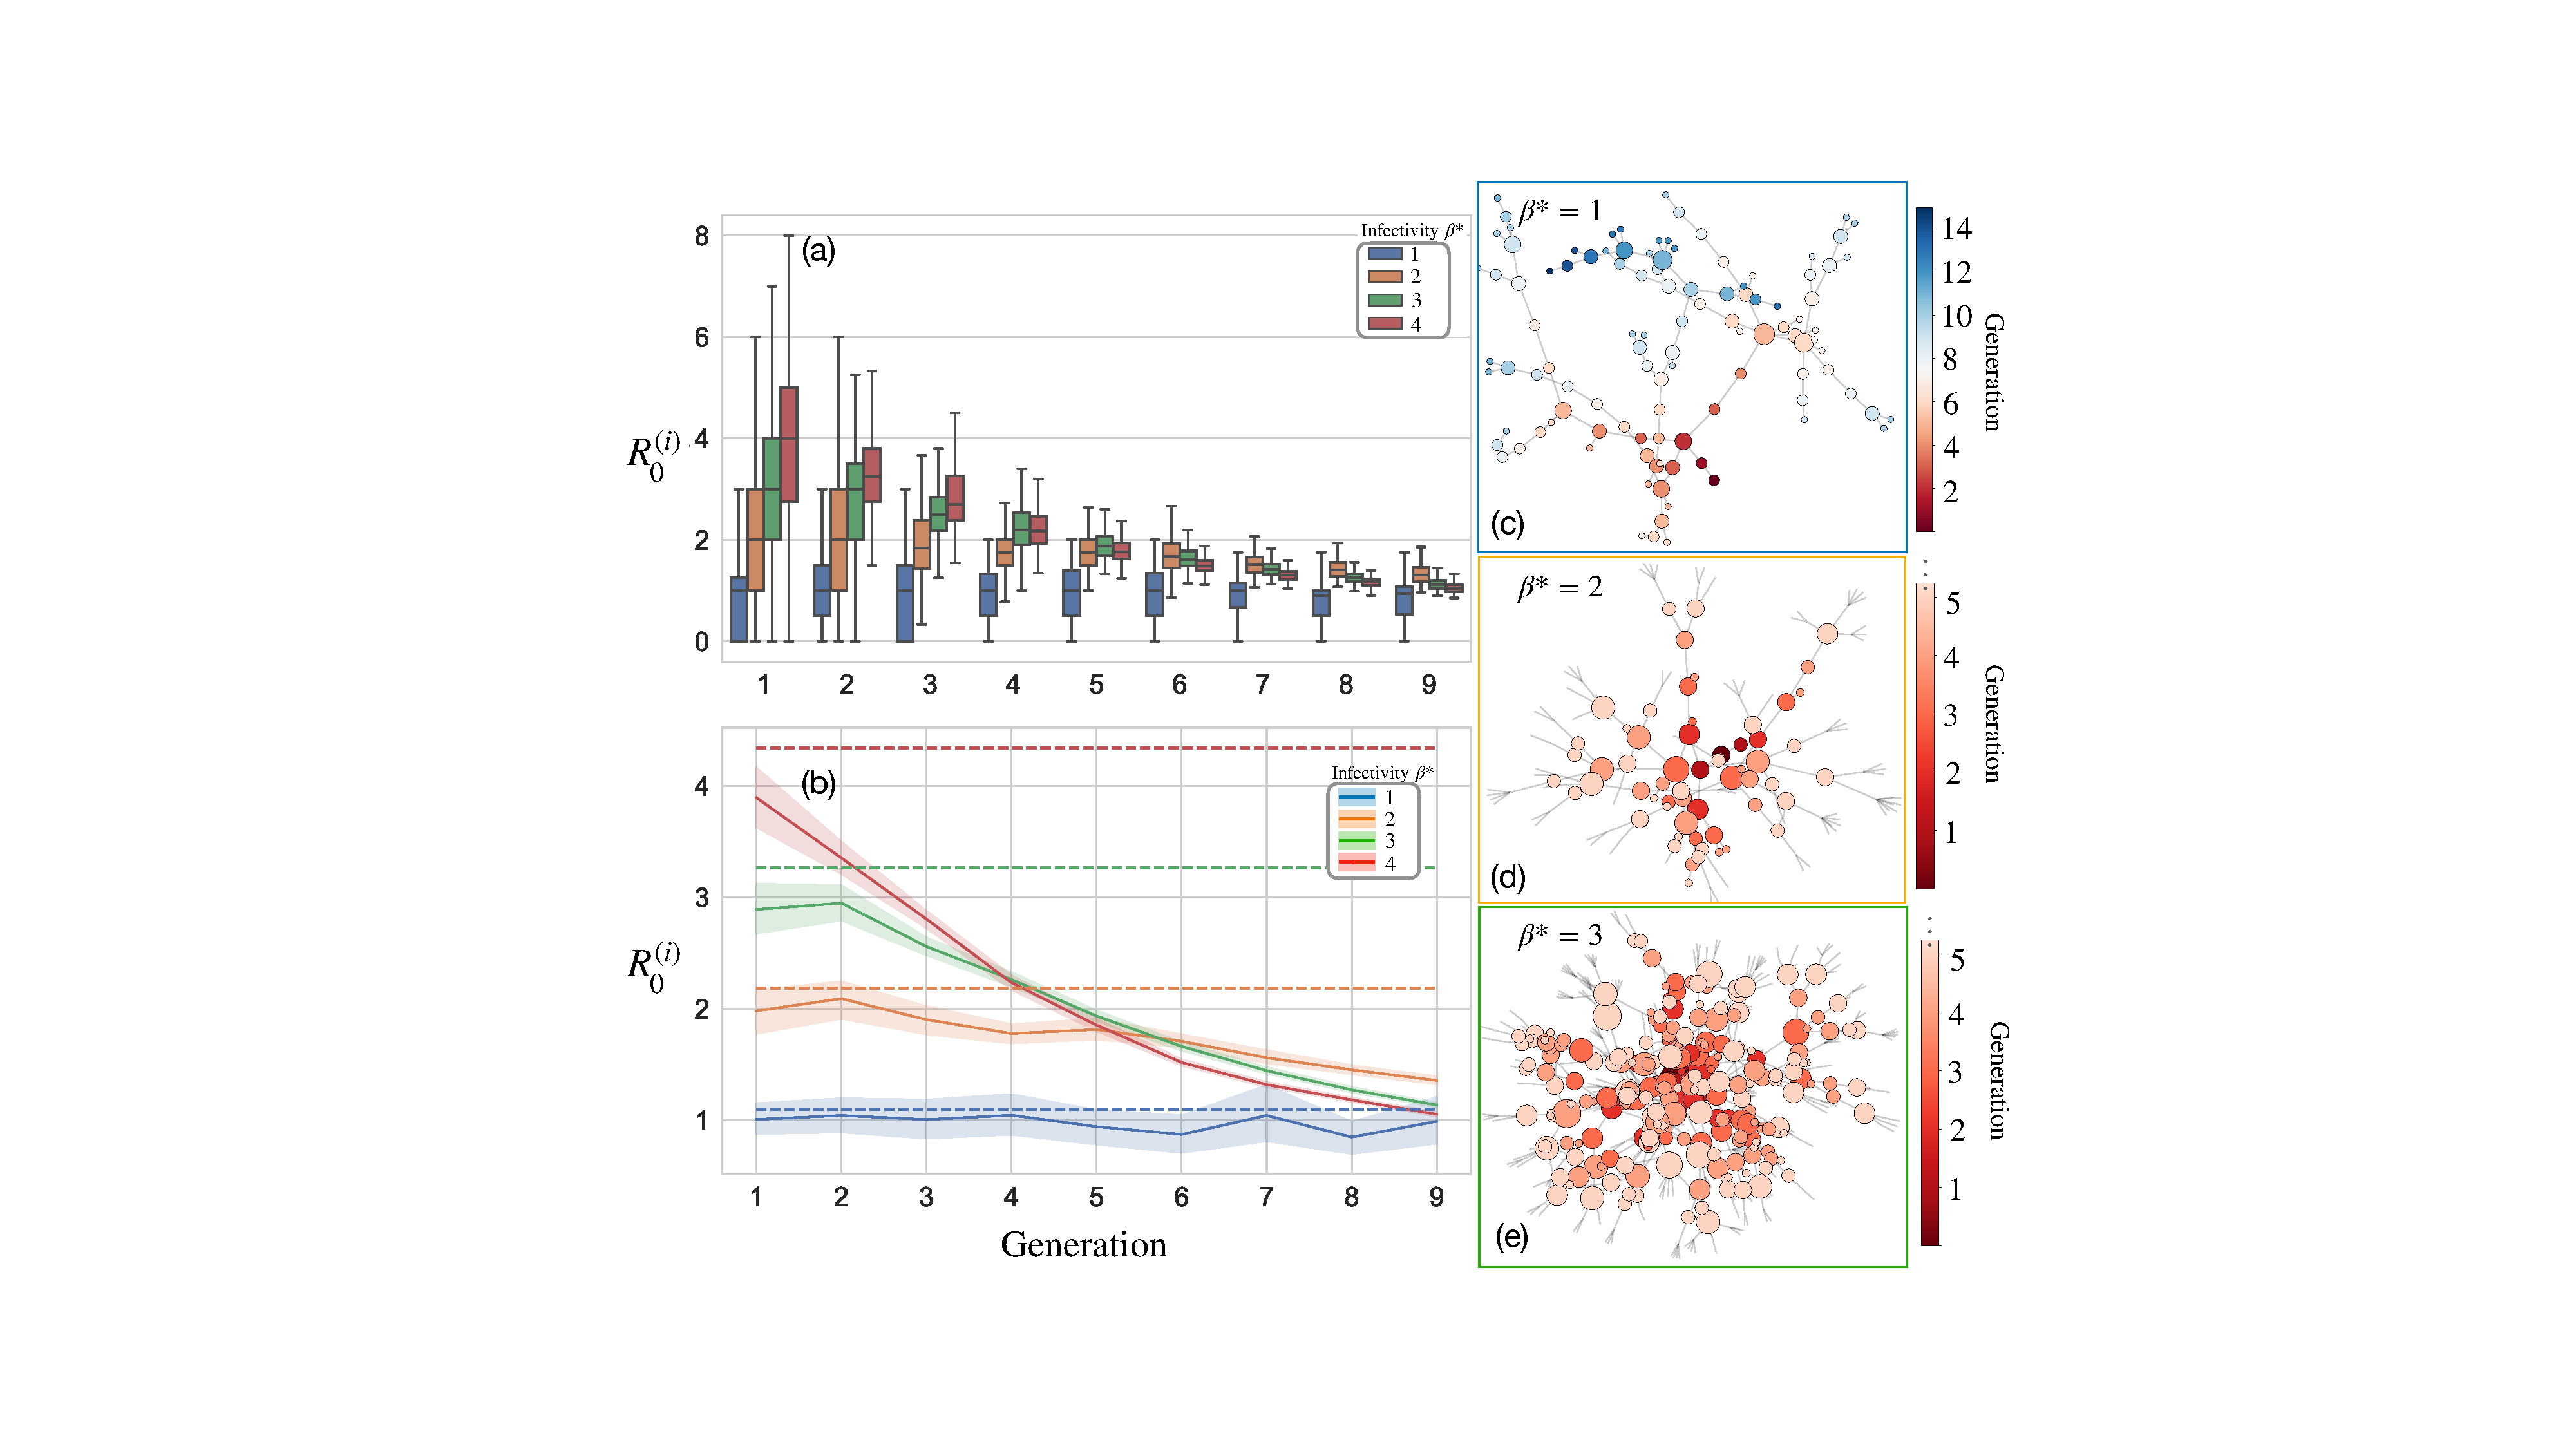
\includegraphics[scale=0.475]{chapter5/figures/fig5-R0-contact.pdf}
    \caption{Contact-tracing mean number of secondary infections for the $i^{th}$ generation of infected trees, $R^{(i)}_0$. For all simulations, tree densities are fixed along with dispersal kernels, ($\rho=0.01$) and $\ell=50$ respectively, inside a domain of size $\mathcal{L \times L} = 500 \times 500$.
    (a) A box and whisker plot showing the mean number of secondary infections plotted over $10$ generations over an ensemble of size $N=500$. Four different infectivity values are shown, from blue to red. (b) The ensemble-mean in (a) is compared against predictions from the analytic expression of $R_0$, plotted as horizontal dashed lines. For early generations, equation \ref{eq:Appendix_final_expression1} agrees well with the contact-traced value of $R_0$ but overestimates the spread for higher infectivities. (c-e) A network diagram representation of typical simulations for parameters $\beta^* \in \lbrace 1, 2, 3 \rbrace $. The nodes' colour and size reflect the generation and number of secondary infections, respectively. As $\beta^*$ is increased, the network quickly explodes\textemdash, thus reflecting the complexity of controlling highly infectious outbreaks.}
    \label{fig:contact-trace}
\end{figure}

Simplistic interactions between trees permit an alternative network representation of disease spread.
In Figures \ref{fig:contact-trace}(c-e), a directed network of disease spread is shown for three typical simulations with infectivity parameters $\beta^* \in \lbrace 1, 2, 3 \rbrace$.
Nodes depict individual trees, while colour and size represent the generation infected and the number of induced secondary infections.
Between two nodes, one edge connects infected generations $n$  and generation $n+1$ (arrows showing the direction are omitted for visual clarity). 
When epidemic parameters are around the threshold, as in Figure \ref{fig:contact-trace}(c), the network appears sparse and chaotic;
whereas Figures \ref{fig:contact-trace}(d-e) show that if infectivity is increased, the network proliferates rapidly. 
Indeed for $\beta^*=2$ and $\beta^*=2$ the network became large if plotted for all generations\textemdash consequently $R_0^{(5)}$ was truncated to permit visualisation.

From Figures \ref{fig:contact-trace}(d-e), one can discern assumptions implicit within the NLM and visualise how targeted epidemic control might be optimised. In the NLM, tree-to-tree interactions are particle-like, meaning that infections spread unidirectionally between two trees at any time. In real life, interactions are more complex. For example, consider two infected trees $(A, B)$ in the vicinity of one healthy susceptible neighbour $C$. Here, infection pressure on $C$ is likely a continuous function of $A$ and $B$. We can collectively represent these more complex interactions by multiple edges between $A, B$ and $C$ in a network representation.
However, the probability of $C$ becoming infected by $A$, $B$ or $A \bigcup B$  occurs with statistical independence. Therefore, we employ the standard method of combining statistically independent events from the inclusion-exclusion formula. 

Although, modelling simultaneous infection pressure from multiple infected trees complicates the definition of $R_0$.
Primarily, infections originate from multiple sources, and we cannot tell from which tree(s) the infection initially spread. See appendix \ref{A:combiniing-probabilities} for a more in-depth discussion on combining probabilities. Nonetheless, another assumption relates to self-loops in the network. In the framework proposed here, trees transition into the $R$ compartment and self-loops are negated. However, in reality, re-infection is possible (e.g. the yearly cycle of ash dieback \cite{gross2014h}) that could be supposed to cause a host's infectivity to increase with each re-infection.

The networks shown in Figures \ref{fig:contact-trace}(d-e) present a simple, yet insightful, representation to gauge what connections epidemic control would need to disrupt.
Well-known results suggest that the scale of control should reflect the spatio-temporal scale of disease spread \cite{control-scale-matching}.
In Figure \ref{fig:contact-trace}(d), even a minimal control effort might disrupt the network well below the threshold of spread,
whereas Figures (d) and (e) would incur an increased effort to stop the spread.
In the network representation, optimised control would involve targeting high priority links between nodes;
this reflects various methods that aim to optimise control by identifying high-risk hosts.


\subsection{Contact-traced $R_0$ and tree mortality}

In Figure \ref{fig:contact-trace-vs-mortality}, the contact-traced value of $R_0$ is compared against the tree mortality, similar to the previous analysis in section \ref{sec:tree-mortality-analytic}.
Figure \ref{fig:contact-trace-vs-mortality} shows an ensemble-averaged reproductive ratio (up to $R_0^{(i=5)}$) plotted against the mean tree mortality, indicated by the dashed curves.
The ensemble mean is then overlaid with a coloured scatter plot depicting a small sample of the data.
Each simulation in Figure \ref{fig:contact-trace-vs-mortality} was repeated $10^3$ times for fixed density $\rho=0.01$, dispersal $\ell=50$ and $\mathcal{L}=500$ over $2500$ time-steps.
As before, a threshold can be witnessed at $R_0^{(i)}=1$, above which tree mortality rises steeply.
For $R_0^{(1)}$, the threshold phenomena witnessed in Figure \ref{fig:contact-trace-vs-mortality} (shown in dashed blue) appears similar to the previous analytic $R_0$ examination.
However, each successive generation appears to define a sharper threshold, especially when $\beta^*$ is high, suggested by the steeper coloured dashed curves.

The steeper thresholds witnessed in Figure \ref{fig:contact-trace-vs-mortality} can be understood
by considering initial stochasticity.
If an outbreak (with high $\beta^*$) does not become extinct at early times, the epidemic is likely to continue to spread until no susceptible trees are left to infect.
Hence, epidemic impact is high and the threshold is sharp for $R_0^{(i)}$, where $i > 1$. 
The reader is referred back to the network diagrams shown in Figure \ref{fig:contact-trace}(d-e) to gain intuition behind this idea;
if the pathogen survives beyond the initial outbreak to establish new centres of infection, the network quickly explodes, and pathogen extinction is unlikely.

The ensemble shown in Figure \ref{fig:contact-trace-vs-mortality} was re-run with $10$ centrally-located initial infections at $t=0$ to test the initial stochasticity.
Intuitively, increasing the number of infected trees reduced early extinction events and subsequently raised the mean tree mortality.
In addition, raising the number of initially infected trees reduced stochasticity in the ensemble and presented a more abrupt threshold in comparison to Figure \ref{fig:contact-trace-vs-mortality}\textemdash more information can be found in Appendix \ref{A:R0-contact-traced-mortality}.

\begin{figure}
    \centering
    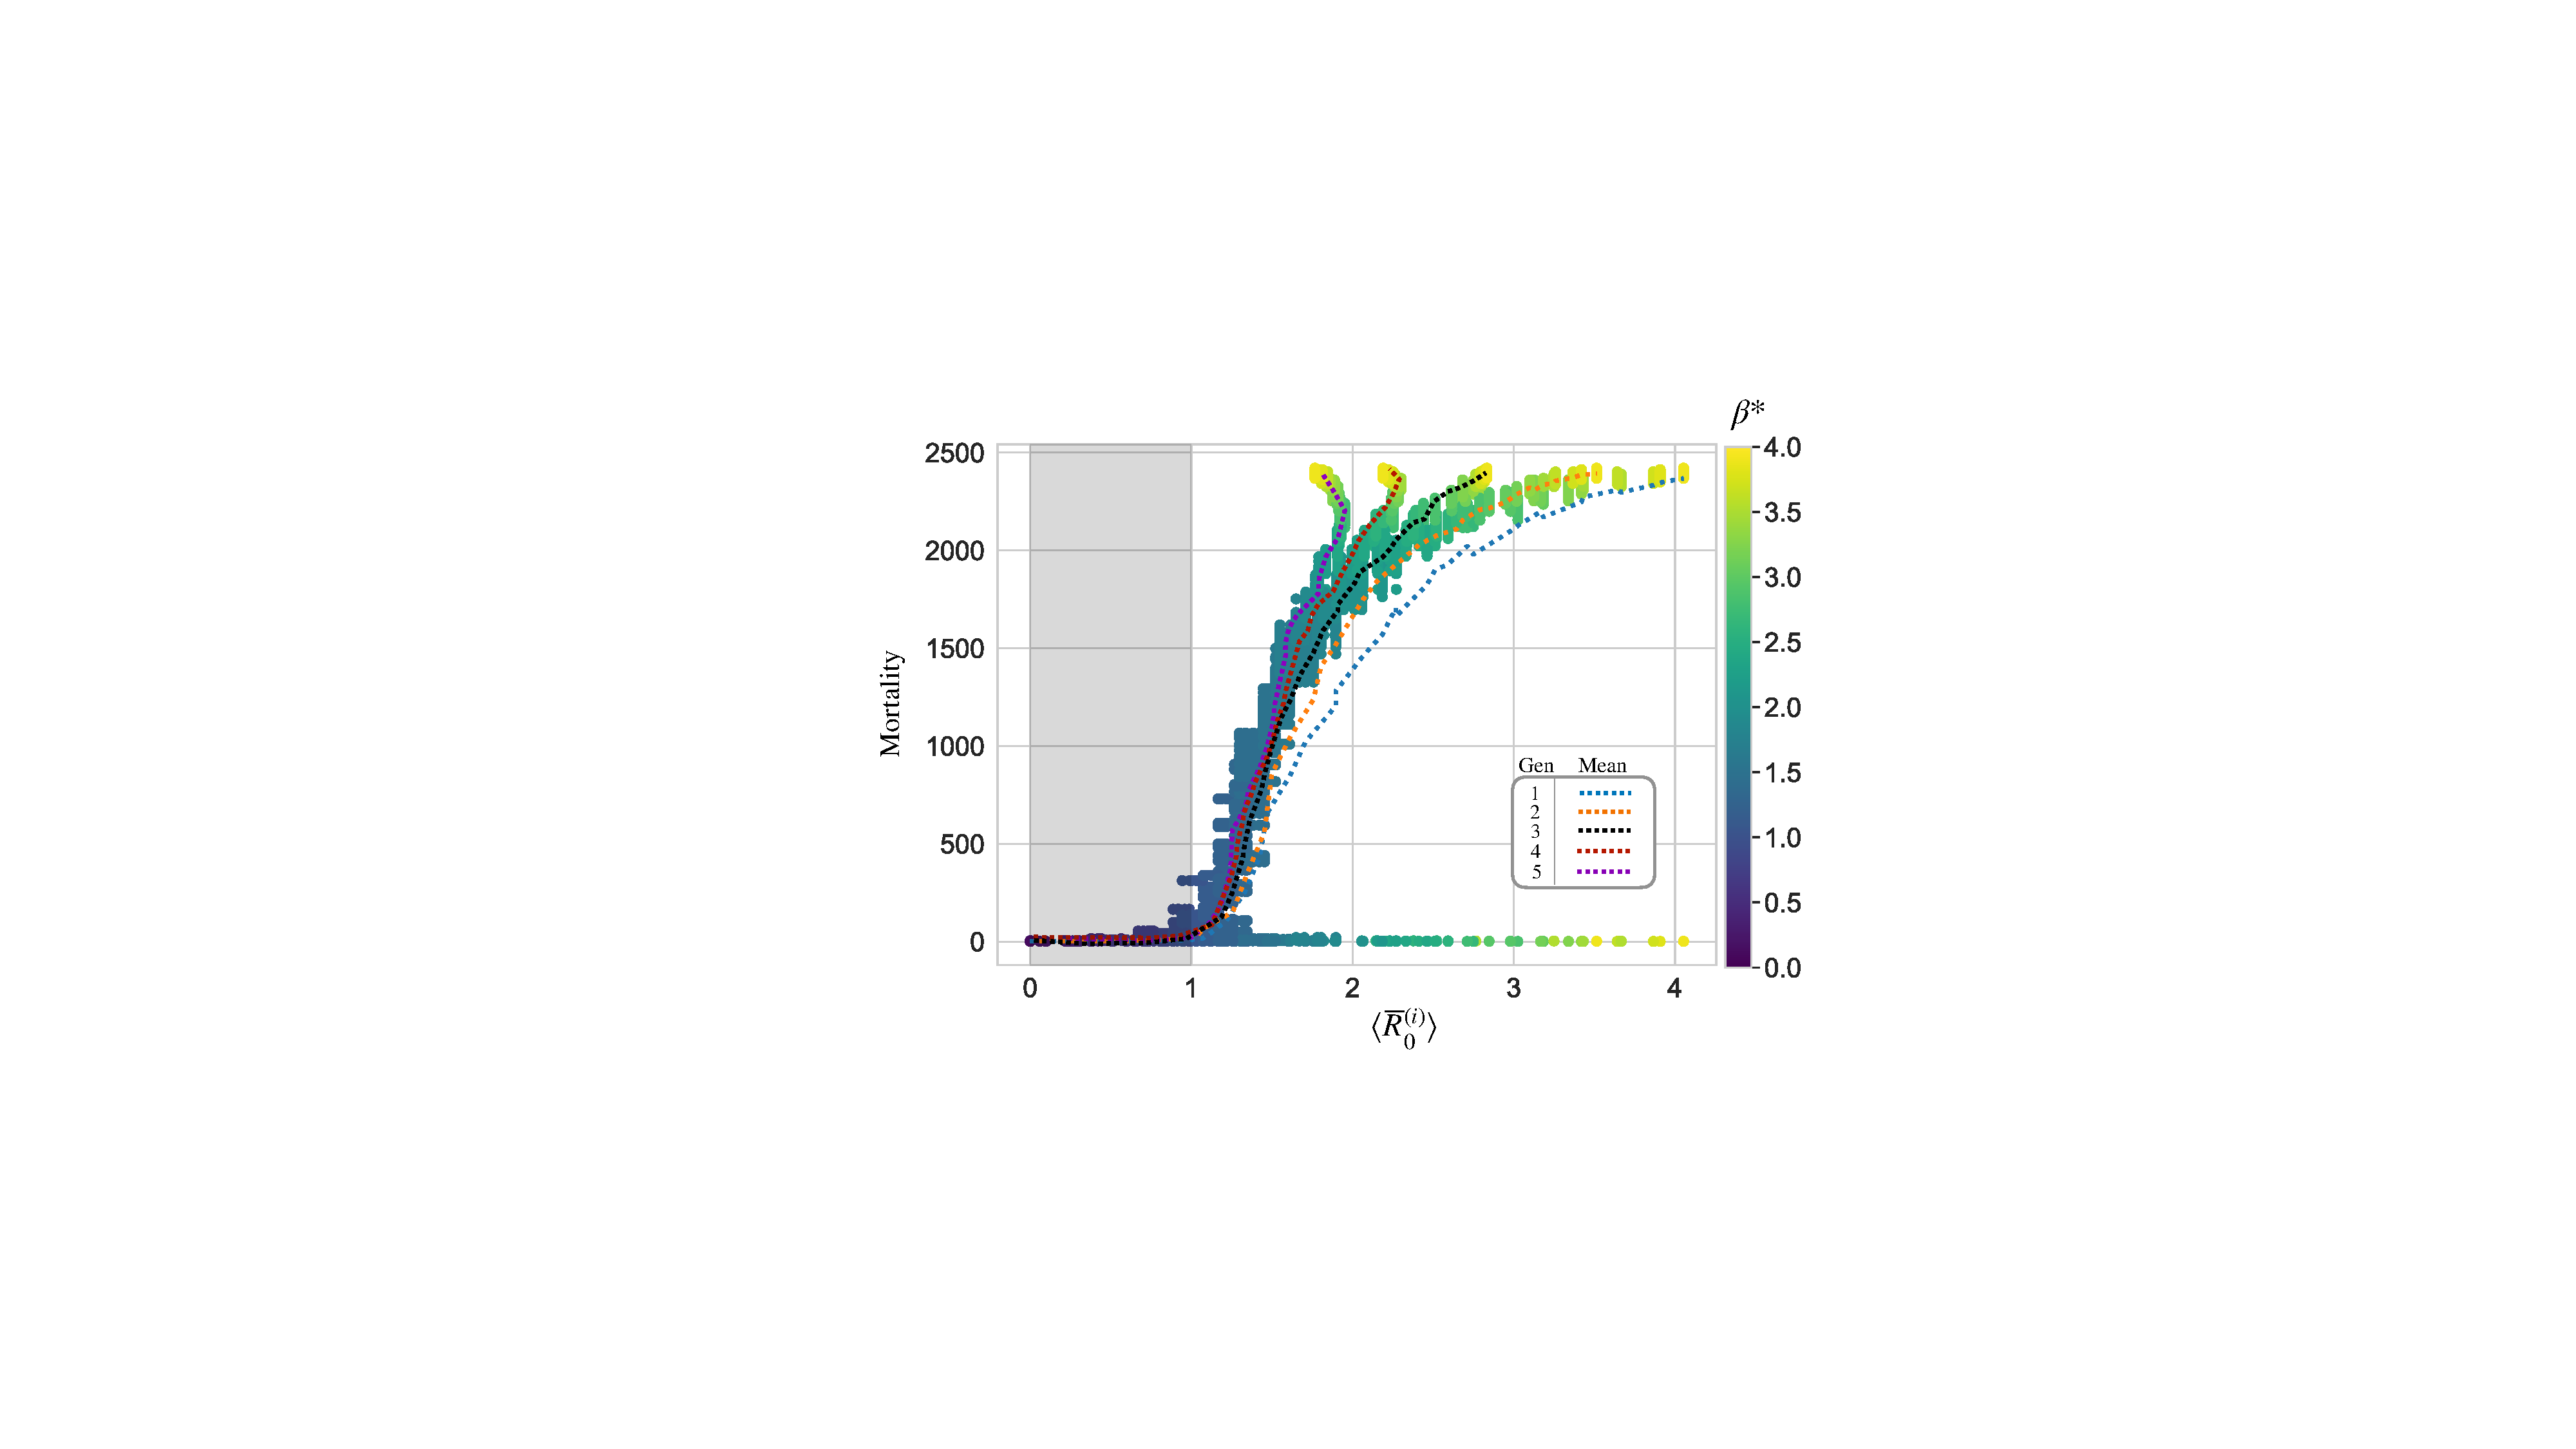
\includegraphics[scale=0.6]{chapter5/figures/fig6-R0-contact-vs-mortality.pdf}
    \caption{Comparing the contact-traced reproduction ratio and the total tree mortality. 
    In each simulation, the tree density and dispersal kernel was fixed to $\rho=0.01$ and $\ell=50$, respectively. 
    For each value of infectivity $\beta^*$, the ensemble-averaged value of $R_0^{(i)}$ is plotted against the mean tree mortality, shown by the dashed curves, for five generations, i.e. $R_{0}^{(5)}$.
    A coloured scatter plot overlays the ensemble-averaged line plots showing a sample of the data\textemdash and also reflecting the value of $\beta^*$.
    As before, a threshold arises around $R_0^{(i)} = 1$, although this time the threshold appears steeper.}
    \label{fig:contact-trace-vs-mortality}
\end{figure}

\newpage
\section{Discussion and future work}

The main aim of this Chapter was to construct a more realistic, dispersal-based model of tree disease.
Hence, a non-local dispersal model (NLM) of tree disease was constructed with SIR compartments and a Gaussian kernel.
Notwithstanding its generic construction, the NLM provides a foundation for the remaining chapters in this thesis.
After describing the NLM, it was compared to the standard SIR framework for a number of dispersal length scales and domain sizes.
Despite some differences, the NLM compared more favourable with the SIR model when the dispersal scale parameter was comparable to the domain size.
Comparisons, therefore, provide compelling indications that spatially-explicit contact-mixing in the tree population may arise with sufficient dispersal.
From this observation, we may question the utility of spatial models for systems where the dispersal length scale is comparable to the size of domain, e.g. when modelling the spread of disease in small fields or plantations. However, comparisons to the SIR model were simplified and limited to one parameter (i.e. the ratio $\beta/\gamma$). As such, the analysis constitutes a preliminary result, and a more sophisticated comparison method is required to glean further insight. For example, a better method of might involve using inference (MCMC methods) to fit the NLM against the standard SIR model.

Two methods of calculating a reproduction ratio, one analytic ($R_0$) and one numerically contact-traced ($R_0^{(i)}$), were outlined to categorize the NLM.
The analytic threshold predicted by equation \ref{eq:Appendix_final_expression1} agreed well with the `actual' contact-traced reproduction ratio computed through NLM simulations,
caveat-ed by the observation that it tends to overestimate $R_0$ when epidemic severity is high.
The overestimation of $R_0$ can be compared to well-known results by \cite{R0-perc-ref, doi:10.1098/rsif.2005.0051},
who showed that the first-generation basic reproduction ratio for farms infected with foot-and-mouth overestimates the growth rate of infection.
In addition, \cite{R0-perc-ref} found that the second generation of infected farms gave a better predictor of the final-sized epidemic (conditional on the epidemic occurring),
thus presenting a clear link to our observation that the tree mortality threshold defined by $R_0^{(i)}=1$ was sharper for later generations.
Crucially, each method of calculating the reproduction ratio defined a threshold around unity, beyond which epidemic impact becomes non-trivial.

An attractive feature of the contact-tracing method, as per definition \ref{def:R0_contact_traced}, 
pertains to its flexibility in the face of more complex spatially explicit models.
Analytical solutions of $R_0$ may become hard to determine for more elaborate life-cycles, dynamics and aggregated host distributions.
Although contact-tracing provides an easy-to-implement method of calculating $R_0^{(i)}$, it should remain, first and foremost, an abstract modelling tool.
For example, consider the immense difficulty of experimentally contact-tracing secondary infections when an epidemic spreads through a forest/landscape.
Contact-tracing the reproduction ratio can therefore be presumed as unobservable in nature\footnote{
We may speculate about measuring a time-varying reproduction number based on the observed numbers of infected hosts,
a well-known concept for characterizing epidemic transmission in human populations \cite{thompson2019improved}.}
However, given sufficient data, one might fit a value of $\beta$ and reverse-engineer a value of $R_0^{(i)}$ from the model;
which leads us to a discussion around the infectivity parameter $\beta$.

A probability of state-change represents infectivity in the NLM, which followed naturally from the percolation model outlined in section \ref{ch3:two-param-model} \cite{OROZCOFUENTES201912}.
However, growth rates are usually employed to describe infectivity\textemdash going back to the original SIR framework \cite{kermack-model} and the logistic growth model of \cite{van2013plant}.
The approach adopted in this Chapter is, therefore, a-typical of contemporary dispersal models based on rates, e.g. \cite{fabre2021optimising, control-theory, white2017modelling, large-scale-control}.
Given that growth rates parameterize most diseases in the literature, the NLM might arguably require a modification towards a rate-based implementation;
however, it must be remarked that sometimes this may not be needed, given that measuring growth rates\textemdash particularly for time-varying infectivities\textemdash is extremely difficult \cite{13-challenges}.
Although unconfirmed, we may suppose an equivalence between the infectivity $\beta$ and an emergent growth rate. This assertion is supported by the similarities exhibited between the NLM and the rate-based standard SIR model in Figure \ref{fig:SIR-fitting} (in addition to appendix \ref{a:exponentially-distributed-lt}).
Nevertheless, presenting $\beta$ as a probability describes an intuitive low-level (microscopic) perspective of disease spread which would, 
in theory, be observable/measurable in reality, in contrast to the $R_0^{(i)}$.
Hence, we may consider infectivity $\beta$ as a fitting parameter.


\newpage


% % 6) A method of control at the landscape level 
\chapter{Constructing $R_0$-maps over Great Britain}
\label{ch:6-adb}

In the last Chapter, we considered a generic $SIR$-based non-local dispersal model (NLM) that spread via a Gaussian dispersal. 
The NLM resolved the major problem witnessed in section \ref{fig:ch4_uk_spread}, 
namely, the failure of the percolation-based model to spread on a realistic host density. 
However, Chapter \ref{ch5:dispersal-model} and the NLM lacked biological specificity. 
Therefore, the present Chapter presents a simplified $SEIR$ model of ash dieback capturing only the essential dynamics of wind-borne dispersal.
Ash dieback (ADB), caused by the fungus \textit{Hymenoscyphus fraxineus}, poses a threat to the survival of European ash (\textit{F. excelsior})\textemdash
the reader is referred to section \ref{ch2:ash-dieback} for a more in-depth discussion of ADB symptoms, life-cycle and management.

In section \ref{sec:seir-model}, a seasonal-based $SEIR$-like model is developed to simulate the natural wind-dispersal mechanism of ADB at local-spatial scales. 
Next, section \ref{sec:seir-behaviour} examines the general pattern of epidemic spread in the $SEIR$ model before section \ref{sec:SEIR-R0-definition} 
outlines a formal definition of an effective reproduction number to measure pathogen invasiveness. 
The effective reproduction number is spatially explicit and based on the same contact-traced method presented in Chapter \ref{ch5:dispersal-model}.
Critically, the wind-dispersal model of ADB rests on $R_0$ measured over an appropriate spatio-temporal scale.

Lastly, in section \ref{sec:r0-map-construct} a framework is developed to spatially-scale $R_0$ values over Great Britain (GB) using a modelled ash canopy cover data-set \cite{hill.data}. 
In effect, this means embedding $R_0$ values from a small-scale epidemic model inside each pixel of an extensive host data set spanning GB, 
thus coupling two models at different spatial scales.\footnote{In general, combining two models at different spatial scales has clear analogies to a 
sub-grid model \cite{sub-grid}, or more recently, a metapopulation-like model \cite{GRENFELL1997395}.} 
Fundamentally, projecting $R_0$ values onto a map of ash densities permits the visualisation of epidemic impact over GB.
The framework is generic and adaptable to any dispersal-based pathosystem, provided a sufficient host density data-set.


The local-scale epidemic model demonstrates that long-distance dispersal (LDD) and long-term survival 
can occur even below the threshold $R_0=1.0$. In addition, analysis at the landscape-level covering GB reveals 
that susceptible clusters of ash grow most rapidly over a narrow range of infectivity parameters, 
presenting behaviour akin to a global epidemic phase transition. % \cite{colizza2008epidemic} can be used as a comparison
Finally, the method developed in this Chapter demonstrates how the epidemic scale can vary significantly, 
albeit with minor epidemic parameter variations. Together, these observations support the call for a risk-based approach to modelling the spread of epidemics in tree populations.

\section{A spatially-explicit seasonal $SEIR$ model}
\label{sec:seir-model}

\textit{H. fraxineus} has two modes of reproduction, sexual and asexual (teleomorphic and anamorphic, respectively).
As some research suggests, the asexual element has contributed to the European epidemic \cite{fones2016role}. 
Although the sexual reproductive mode of ADB is widely acknowledged to be the dominant driver of disease-spread 
\cite{https://doi.org/10.1111/ppa.12844, havnavckova2017direct, gross2012reproductive, Timmermann2011elal}.
Subsequently, only the sexual reproduction of \textit{H. fraxineus} is reflected in the $SEIR$ model.

The entire sexual reproductive cycle occurs on ash leaves, yet the fungus will spread through ash hosts once infected. 
As such, the precise sexual reproductive mode presents a peculiar modelling scenario where both leaves and trees can be argued
to host the pathogen \textit{H. fraxineus}. 
Typically, leaf dispersal emanating from a large deciduous tree species (such as \textit{H. fraxineus}) remains close
to the tree trunk and rarely exceeds $30\mathrm{m}$ \cite{nickmans2019modelling}. Hence, leaf litter is assumed to fall close
to infected trees to treat both ash hosts and infected litterfall at the same lattice position in the model. 
A more intricate model of ADB could aim to relax this assumption and describe autumn leaf-shed with a suitable leaf-fall dispersal kernel\footnote{
    Patterns of leaf fall are vital for ecosystem nutrient recycling \cite{staelens2003model}. 
    Leaf-fall dispersal kernels have been collected (and modelled) for oak, beech, hornbeam and birch \cite{nickmans2019modelling},
    although despite a detailed search, no such dispersal kernel for ash could be found.
}.

\subsection{Infection dynamics}
\label{sec:infection-dynamics}

The infection dynamic comprises four states: susceptible $S$, latently infected $E$, infectious $I$ and removed $R$
that transition through $S\rightarrow E \rightarrow I \rightarrow R$ without the possibility of recovery.  
Figure \ref{fig:SEIR-transitions} shows a typical scenario where an infected ash tree in the $n^{th}$ cycle (or equivalently $n$ 
years after the initial outbreak) can infect ash in the $S$ compartment. A newly infected ash transitions into the $n^{th}$ $E$ compartment at time $t$, 
denoted by $E_n$, and becomes infectious in the following year $I_{n+1}$. The distribution of susceptible ash is described by 
the same flat randomly distributed population of trees used previously in Chapters 3-5.

\begin{figure}
    \centering
    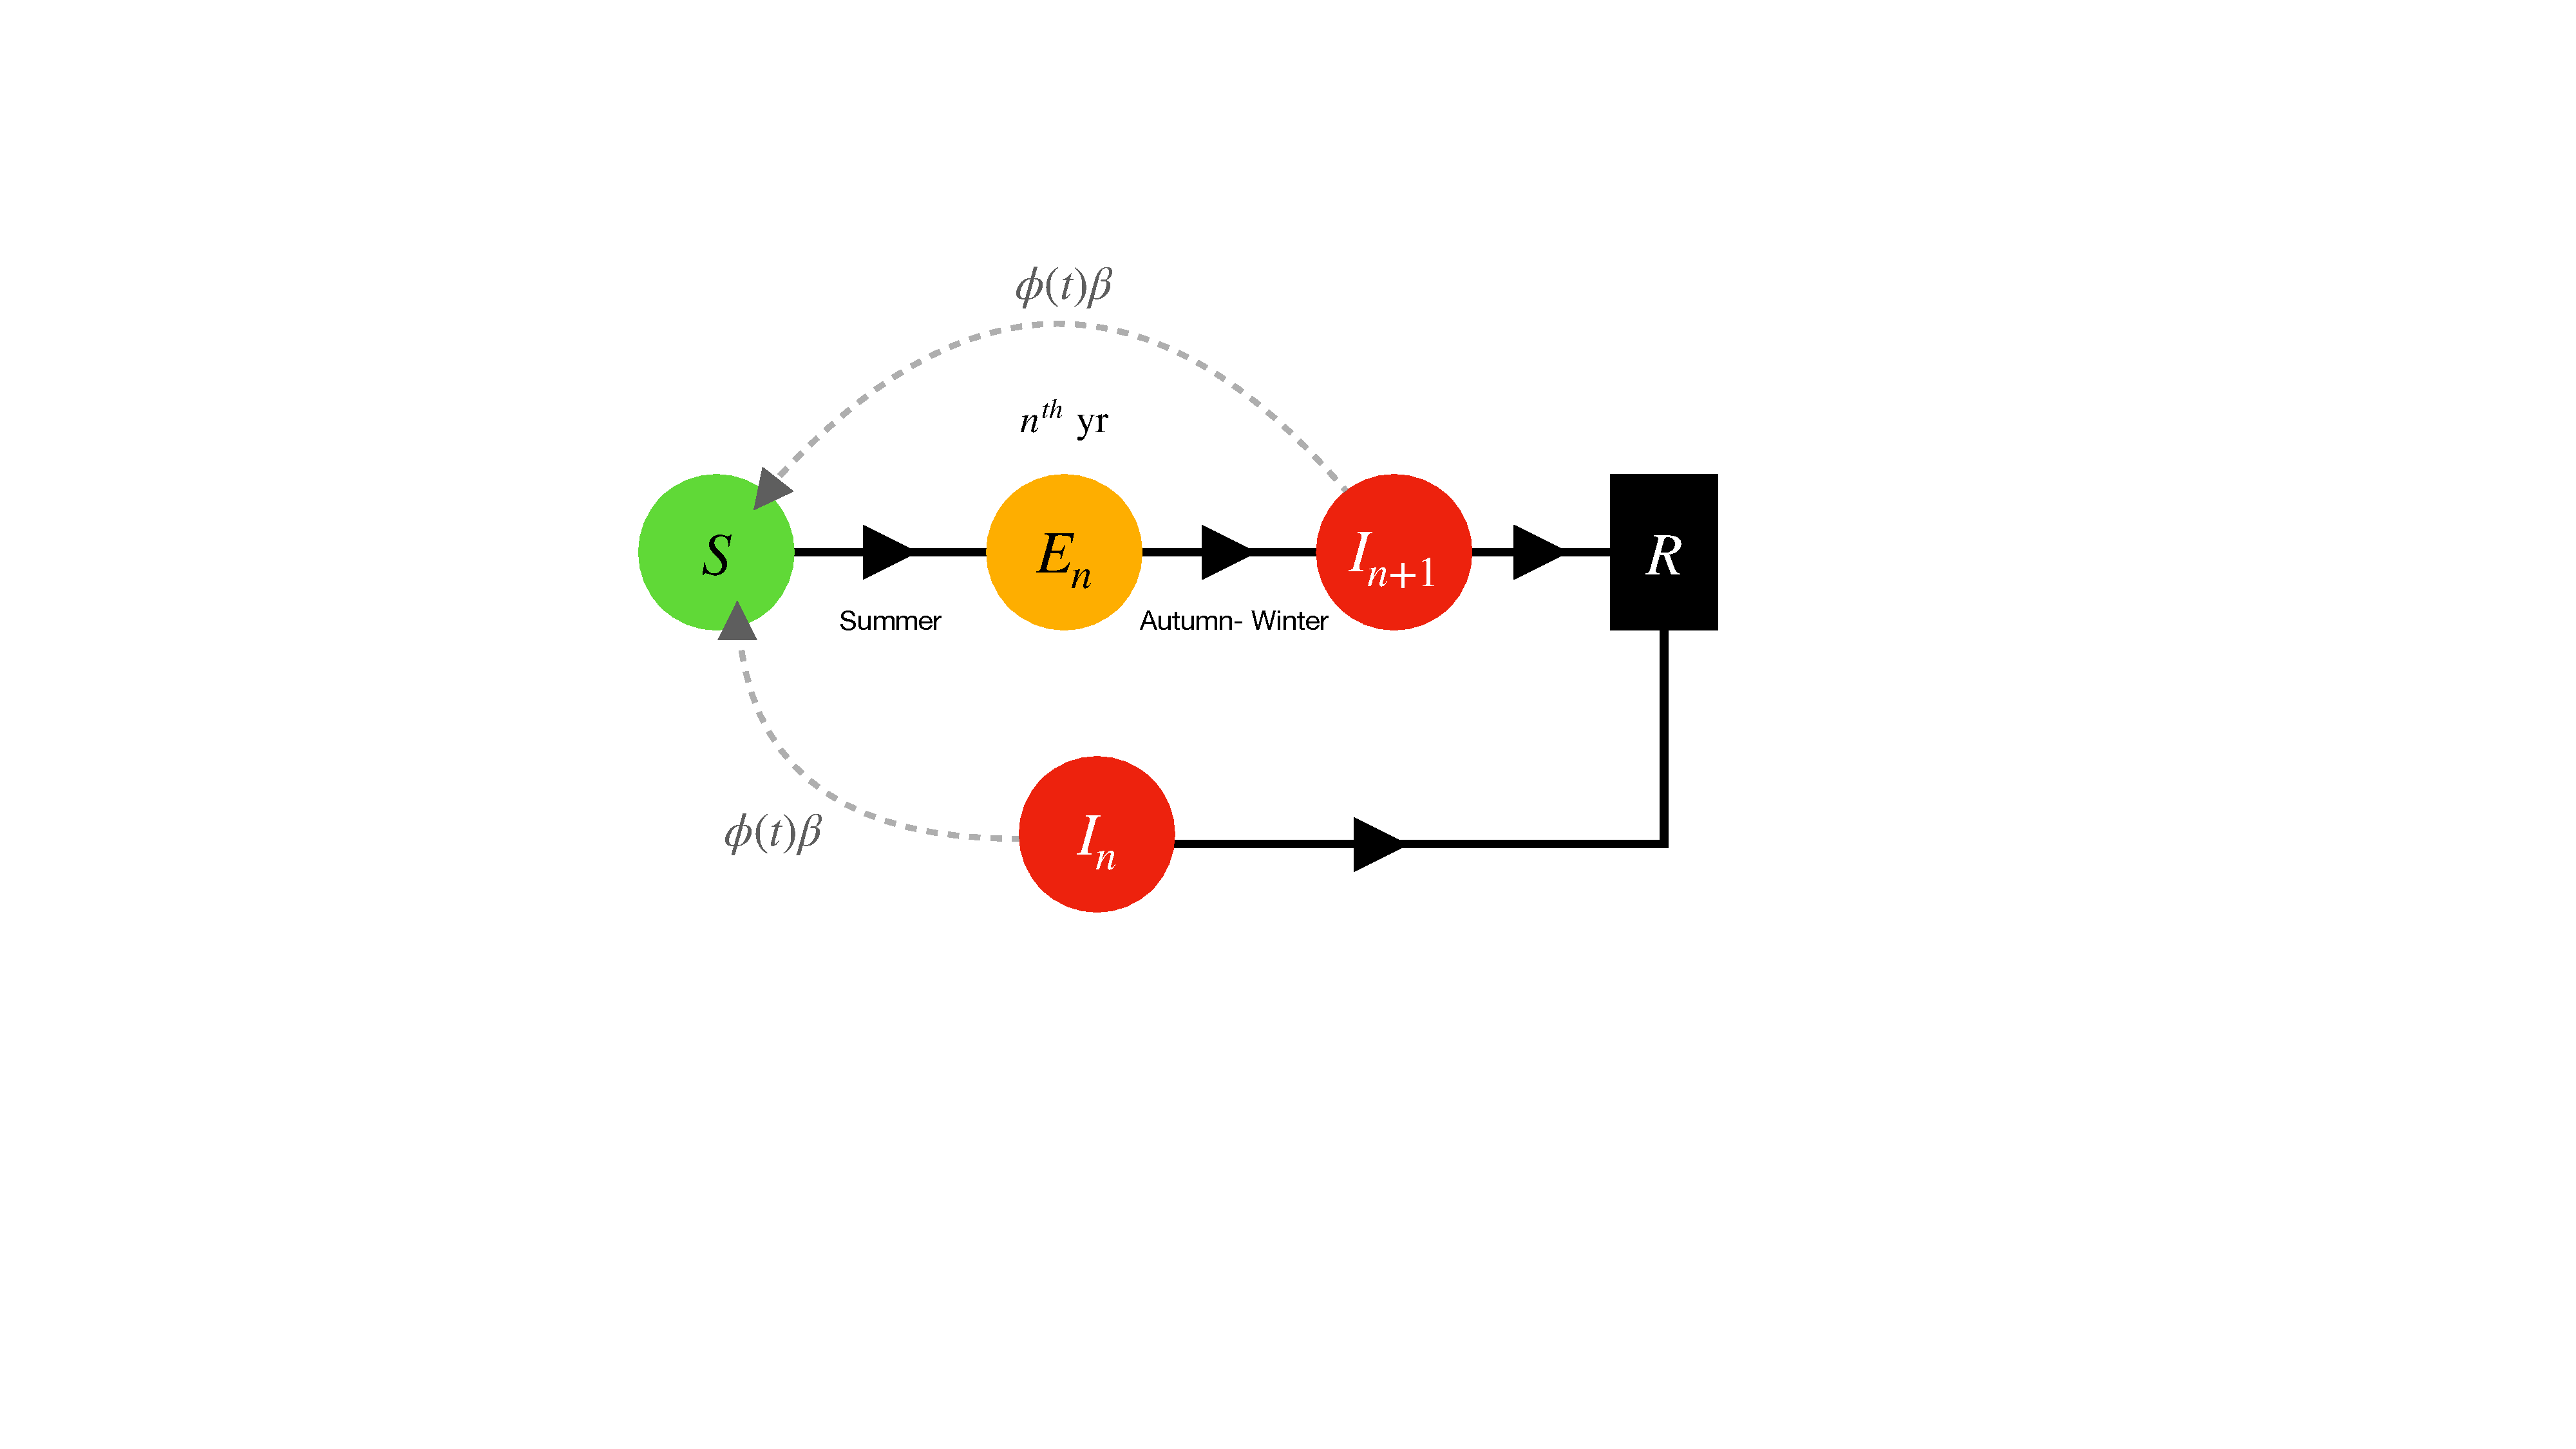
\includegraphics[scale=0.40]{chapter6/figures/fig1-seir-transitions.pdf}
    \caption{The seasonal $SEIR$ model of ADB. (a) In year $n$ of an outbreak, an infectious tree may cause a transition $S\rightarrow E_n$ during summer, 
             depicted by the bottom dashed grey arrow. A tree that becomes latently infected in year $n$ will lead to an infectious tree in year $n+1$. 
             Eventually, all infected ash are removed without the possibility of recovery. 
             (b) The yearly cycle of the pathosystem ADB. Leaf-flush coincides with the sporulation season. 
             Sporulating fruiting bodies release ascospores between June-September. Ash shedding takes place from late summer-early winter.}
    \label{fig:SEIR-transitions}
\end{figure}

Here, each lattice point in the $L\times L$ domain is chosen to represent a $5\mathrm{m}\times5\mathrm{m}$ patch of land
that approximates the canopy cover of an average ash tree\textemdash although young saplings usually assume less area. 
A domain resolution of $5\mathrm{m}\times5\mathrm{m}$ yields an upper bound of $400$ ash trees per hectare of canopy cover, 
indicative of densely populated ash stands \cite{ash-tree2, ash-tree1}.

\subsubsection{Transitions: $S\rightarrow E_n$}

Individual tree-to-tree interactions are modelled as a system of particles (introduced previously in Chapter \ref{ch5:dispersal-model}).
Transitions from $S$ to $E$ involve two components: a time-varying infectivity $\beta\phi(t)\in [0, 1]$ and dispersal function $D(r; \ell)\in [0, 1]$.
A thin-tailed Gaussian was considered alongside a normalisable fat-tailed inverse power law distribution to model dispersal.
We assume that in year $n$, ash located at position $x$ can transition into the exposed category under the influence of infected
ash located at $x^\prime$, denoted by $S_x \rightarrow E_{x,n}; I_{x^\prime, n}$.
For an infected tree that remains infectious during the step $t\rightarrow t + \delta t$, the probability of transition follows:
\begin{equation}
    Pr(S_{x} \rightarrow E_{x,n} ;\ I_{x^{\prime}, n} ) = \beta  \phi(t) D(r;\ell)
\end{equation}
where $r$ is the distance between $x$ and $x^{\prime}$, and $\phi(t)$ is a time-dependant function reflecting the seasonal life-cycle of ADB, 
henceforth referred to as a \textit{sporulation function}. Following the method outlined in Chapter \ref{ch5:dispersal-model}, 
transition probabilities are calculated at each time-step, taken to be days, while trees are infectious.

\begin{table}
\centering
    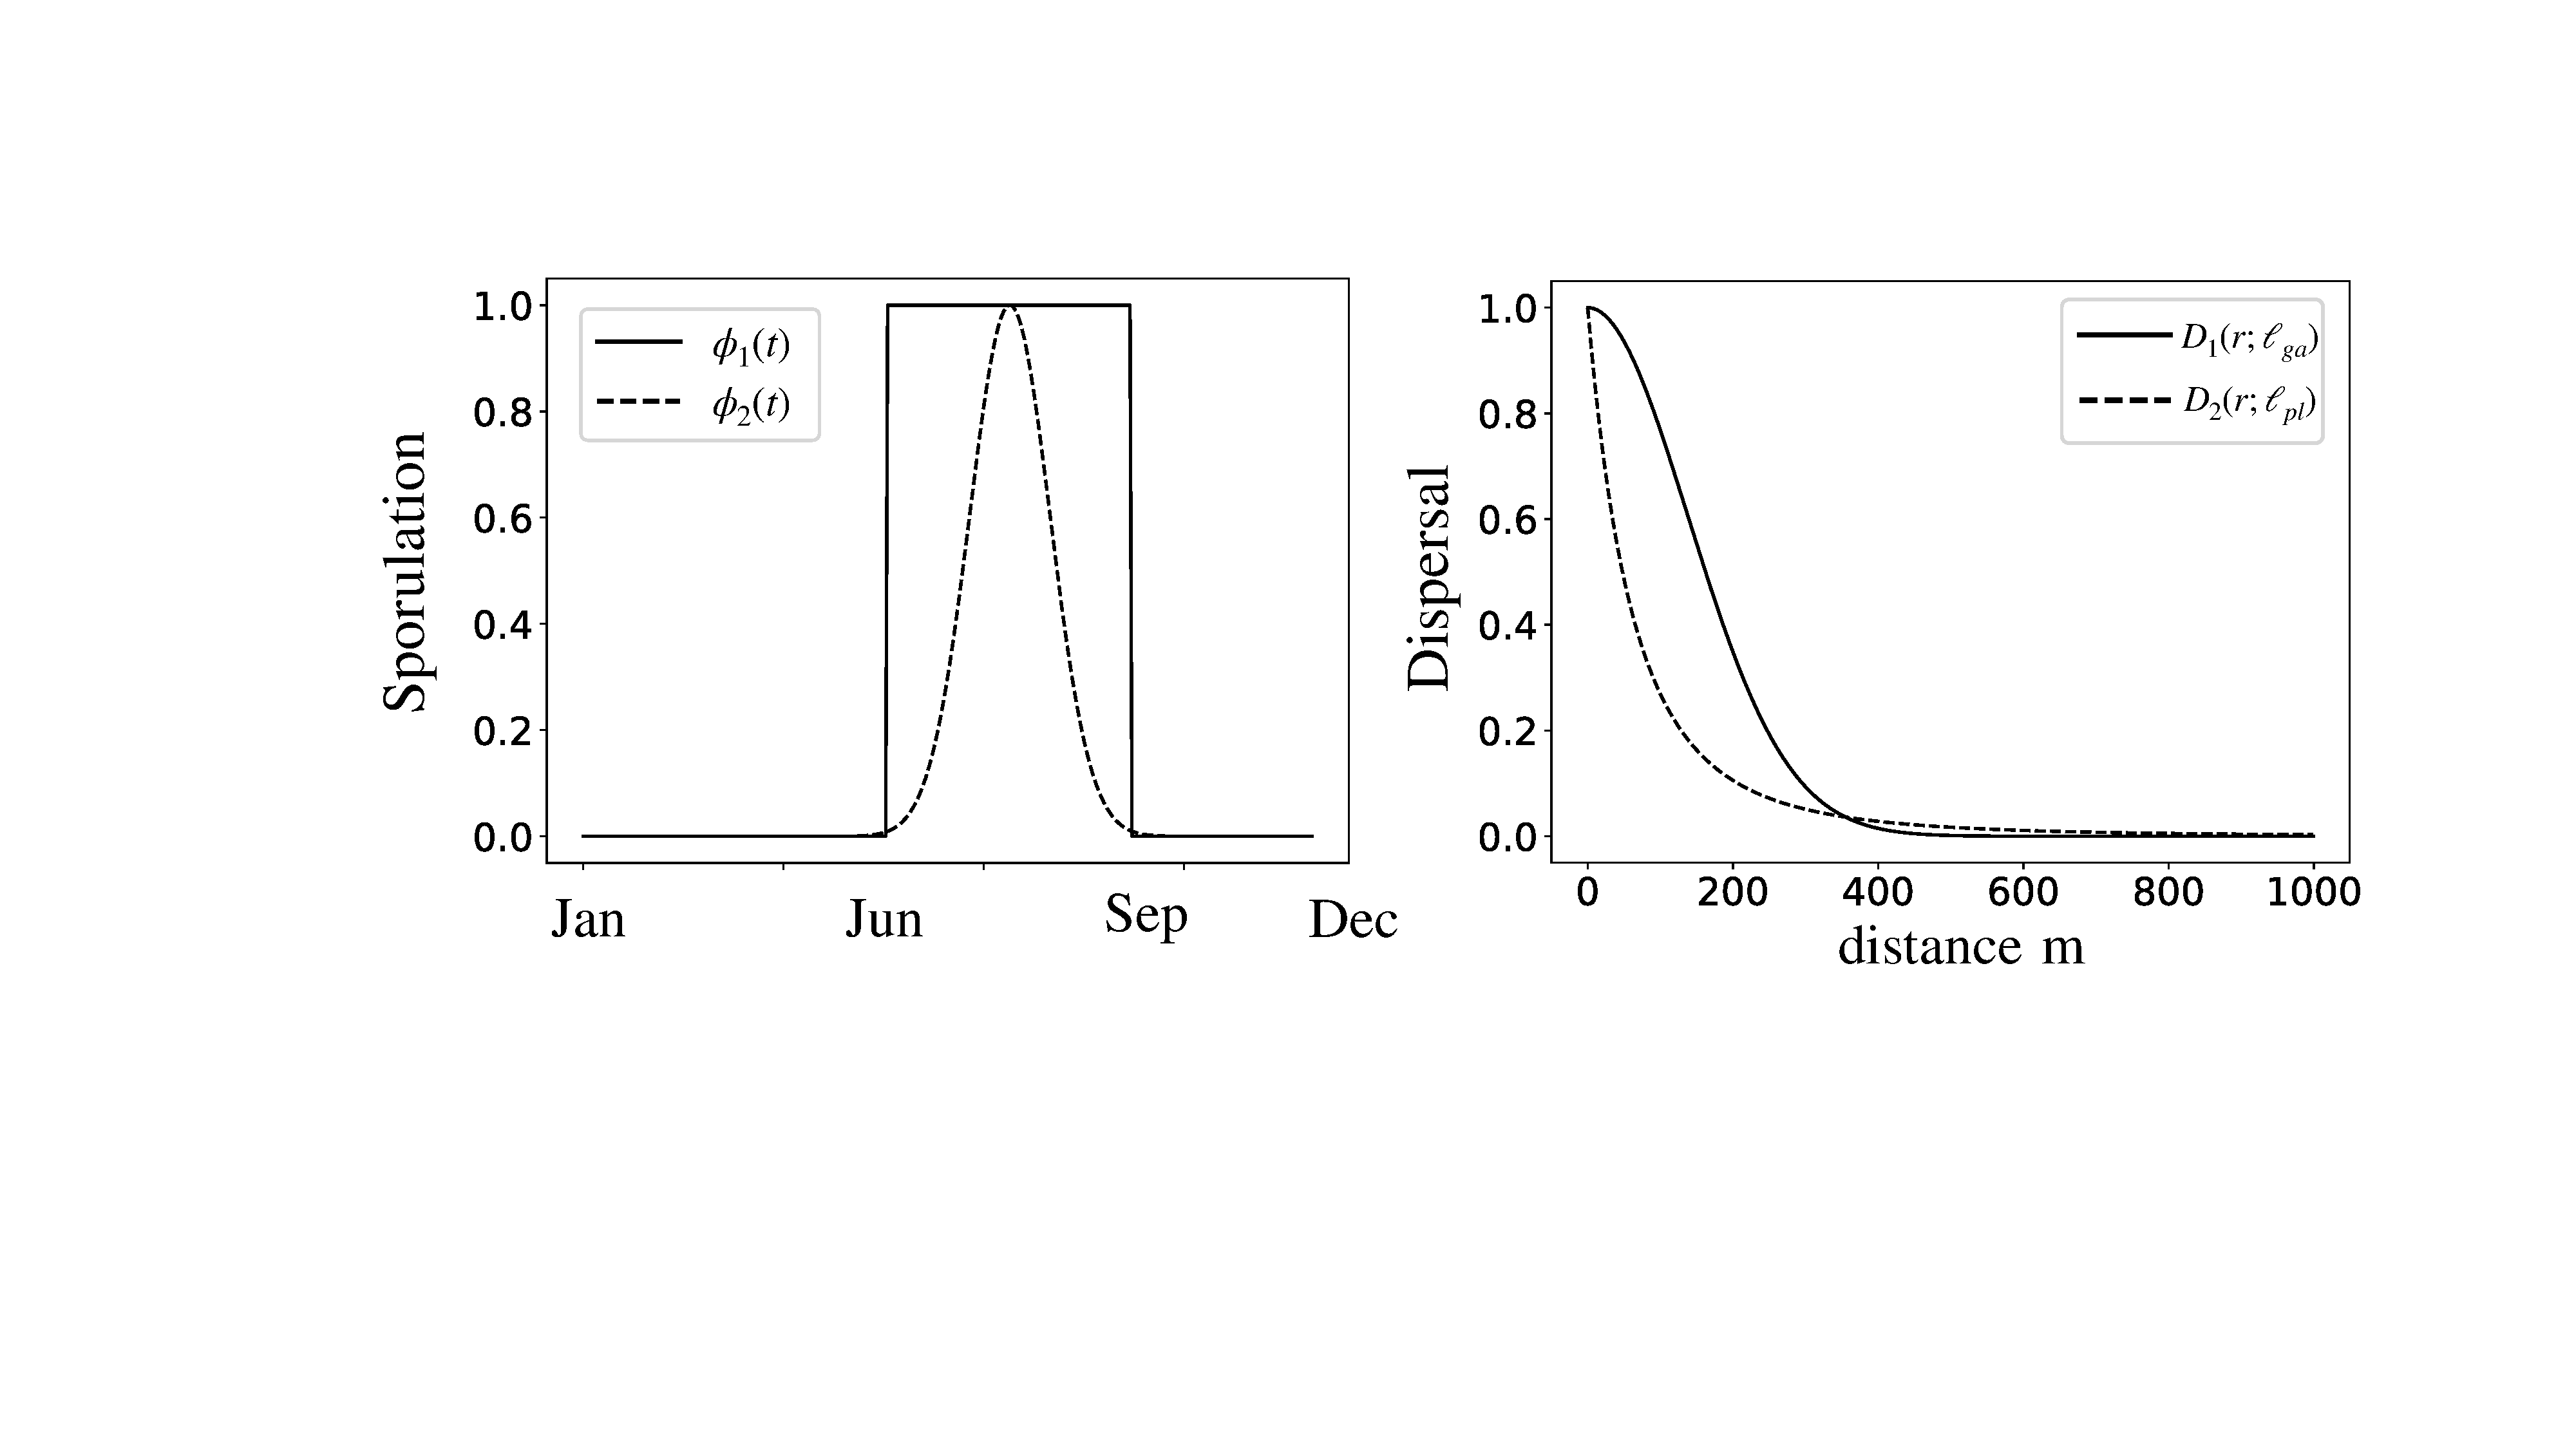
\includegraphics[scale=0.3]{chapter6/figures/fig-phi-disp.pdf}
\begin{tabular}{ m{2.3cm}  m{7cm}  m{4.cm} }
 \\
 \hline
 Model name &  \hspace{3em} $Pr(S_{x} \rightarrow E_{x,n}; I_{x^{\prime}}) \in [0, 1]$ & \hspace{2em} $\beta^*$ factor\\
 \hline
 1: $\phi_1$-ga & 
 \[= \left\{
\begin{array}{ll}
      \beta  \exp\Big[-\frac{r^2}{\ell^2_{ga}}\Big] &  t \in [\mathrm{June,\ September}] \\
      0 & \hspace{2.75em}\mathrm{otherwise} \\
\end{array} 
\right. \] & 
\[ 
\frac{1}{T} \frac{1}{\pi\ell_{ga}^2}
\]  \\
 2: $\phi_1$-pl & 
 \[   = \left\{
\begin{array}{ll}
      \beta  \big[1 + \frac{r}{\ell_{pl}}\big]^{-a}  &  t \in [\mathrm{June,\ September}] \\
      0 & \hspace{2.75em} \mathrm{otherwise}
\end{array} 
\right. 
\] 
& 
\[
\frac{1}{T} \frac{(b-1)(b-2)}{2\pi\ell_{pl}^2}\]
\\
3: $\phi_2$-ga & 
\[ 
  =  \beta \exp\Big[-\frac{(t - T_{SP})^2}{2\sigma_{SP}^2}\Big] \exp\Big[-\frac{r^2}{\ell^2_{ga}}\Big]
\]  
  & 
\[ 
\frac{1}{\sqrt{2\pi}\sigma_{SP}} \frac{1}{\pi\ell_{ga}^2}\]
\\
4: $\phi_2$-pl & 
  \[ 
  =  \beta \exp\Big[-\frac{(t - T_{SP})^2}{2\sigma_{SP}^2}\Big] \big[1 + \frac{r}{\ell_{pl}}\big]^{-a}
\]  
  & 
\[ 
\frac{1}{\sqrt{2\pi}\sigma_{SP}} \frac{(b-1)(b-2)}{2\pi\ell_{pl}^2}\]
\\
 \hline
 \end{tabular}
  \caption{Four infection models are considered, composed of either: Gaussian (ga) or inverse power law (pl) dispersal, and step function ($\phi_1$) or peaked ($\phi_2$) sporulation. All component functions yield values in the interval $[0, 1]$ and are normalisable. The corresponding model parameters are shown below in Table \ref{tab:SEIR-model}. 
  The right-hand column shows the normalisation factor used to construct $\beta^*$, i.e. to fix epidemic-impact between models.}
\label{tab:model-variants}
\end{table}

\begin{table}[h]
\centering
\begin{tabular}{l l l}
\hline
\textbf{Model parameter} & \textbf{Description} & \textbf{Value(s) taken}\\
\hline
$\rho$  & Tree density & $0.00 - 0.10$ \\ 
$\beta$ & Infectivity & $0 - 10^{-3}$ \\
$\ell_{ga}$ & Gaussian scale parameter $=\sqrt{2}\sigma_{ga}$ & $196\mathrm{m}$ \\
$\ell_{pl}$ & inverse power law scale parameter & $203\mathrm{m}$ \\
$a$ & Inverse power law exponent & $3.3$ \\
$t$ & Time-step & $1\ \mathrm{day}$\\
$T$ & Days in Sporulation peak June - September & 122  \\
$T_{SP}$ & Peak sporulation $\phi_2$ & end of July \\
$T_{LS}$ & Peak ash leaf-shedding & mid-November \\
$\alpha$ & Lattice constant & $5\mathrm{m}$ \\
$L$ & Lattice dimension (i.e. an $L\times L$ patch)  & $200$ - $2000$ \\
$A$ & Domain area (defined by $\alpha L\times \alpha L$) & $1\mathrm{km^2}$ - $20\mathrm{km^2}$ \\
$\lambda$ & Mean infectious life-time & $5\ \mathrm{years}$ \\
$R_0$ & Mean reproduction number & $0-20$ \\
\hline
\end{tabular}
\caption{Parameters used in the $SEIR$ model of ash dieback. The dispersal parameters are taken from \cite{grosdidier2018tracking} and the typical tree densities of ash are informed from by \cite{hill.data}.}
\label{tab:SEIR-model}
\end{table}

The sporulation function $\phi$ dictates when infectious trees in $I_n$ produce new secondary infections. 
For ADB, sexual reproduction repeats yearly from June to September during its \textit{`sporulation season'}.
As such, $\phi$ is non-zero during the sporulation period.
Two sporulation functions are considered, $\phi_1$ and $\phi_2$, based on the step function and normal distribution, respectively.
Sporulation is developed later in section \ref{ch6:sporulation}, alongside the precise functional form of $\phi_1$ and $\phi_2$.
Altogether there are four infection models, summarised in table \ref{tab:model-variants}.

Once in the $E$ compartment, trees are infected but not infectious, i.e. latently infected.
For example, ash infected with \textit{H. fraxineus} take approximately two weeks to display 
symptoms \cite{https://doi.org/10.1111/ppa.12048, https://doi.org/10.1111/ppa.12844},
and start to shed infectious leaves in following autumn after infection \cite{gross2014h}.
The sub-compartments $(E_1, E_2,..,E_n)$ represent the same biological state of latently infected,
the index $n$ is merely included for convenience to highlight the fact that in this model, 
the mean latent period is one year and new secondary infections are produced during the $(n+1)^{th}$ sporulation peak\textemdash as elaborated in section \ref{sec:En-In+1} below.

\subsubsection{Transitions: $E_n\rightarrow I_{n+1}$}
\label{sec:En-In+1}

As defined here, latently infected trees (in $E_n$) transition into the infectious compartment ($I_{n+1}$) during their 
first seasonal leaf shedding following infection, between autumn and winter.
Then, infected ash trees disperse infectious leaf litter each year following infection until its eventual demise. 
This dynamic assumes that all ash are susceptible and \textit{H. fraxineus} spreads to the xylem after infecting ash leaves.
In reality, a variety of genetic and environmental factors determine the ability of ADB to invade an ash\footnote{
The pathogen \textit{H. fraxineus} can infect ash leaves regardless of tolerance. 
However, only the minority of tolerant individuals can prevent inoculum from spreading to the xylem.}.

A Gaussian distribution represents the onset of ash leaf-shed, and therefore the transition $E_n\rightarrow I_{n+1}$.
Leaf-shed repeats yearly, centred in mid-November (denoted by $\sigma_{LS}$) with a two-week standard deviation ($\sigma_{LS}$) 
and repeats yearly. Centring the normal distribution in mid-November, with a two-week standard deviation, ensures that the earliest
possible onset of leaf-shed (described by the left-hand tail) begins in September.
In the field, the timing of ash shedding their leaves is more complicated and depends on tree age. 
Observations by \cite{hietala2013invasive} suggest that younger ash begin to defoliate in late August,
while large dominant ash starts to shed in early October.

Despite a thorough search, research on ash litterfall distributions appears absent from the literature, 
so choosing a normal distribution centred in mid-November with a two-week standard deviation is ultimately ill-informed. 
Nevertheless, selecting a normal distribution is supported by observations of leaf litter-fall in deciduous 
forest \cite{zhang2014seasonal, dixon1976analysis}, which typically follow peaked distributions that repeat yearly\footnote{
    For example, research conducted on wetland forests in South Carolina demonstrates that the temporal pattern of litter-fall
    peaks yearly between August and November, albeit with some variation \cite{shure1985litter}.}.
That said, within the $SEIR$ model, a time delay exists between the transition $E_n \rightarrow I_{n+1}$ in autumn/winter and the 
sporulation function $\phi(t)$ becoming sufficiently large in summer; so we can afford some degree of flexibility in the exact time scale.
From a mathematical standpoint, provided that latently infected ash transitions into the infected compartment before the sporulation season,
the epidemic spread in this model will remain the same.

% The seasonal pattern of litter-fall plays an important role in ecosystem function and forest health. 
% taking into account more involved leaf-shed dynamics
% A more complex model of ADB, involving soil-borne interactions, could incorporate the build up infected leaf biomass into a time-varying $\beta$. 
% However, it remains to be seen if this is necessary to capture the essential dynamics of wind-borne dispersal.

\subsubsection{Transitions: $I_n\rightarrow R$}
\label{sec:I-to-R}
The last transition to consider is from infected to removed $I_{n}\rightarrow R$. 
Given a $95\%$ mortality rate, ADB can be regarded as lethal \cite{ash-dieback-costs}. 
Therefore, we assume an eventual transition to the $R$ compartment once an ash tree becomes infected.
As mentioned above, the picture is more complex in reality. 
For example, stress-free trees in urban settings can survive for long periods if pruned \cite{marciulyniene2017can}, and a low minority of healthy tolerant trees can fight off the infection.
Additionally, other outlying edge-cases can contradict this assumption, including
laboratory experiments that have shown leaf-shed can result before the infection has the chance to spread through to the petiole following a \textit{`massive ascospore inoculation'} \cite{https://doi.org/10.1111/mpp.12073}.

Ash dieback affects trees of all ages, with younger ash being more susceptible while larger, mature ash appear more tolerant. 
As a first approximation, infected ash trees were chosen to have exponentially distributed lifetimes with a mean of five years, see table \ref{tab:SEIR-model}.
Experimental observations of ash mortality after years of infection support this decision. 
In particular, reports of $5\%$ mortality after two years of infection \cite{kessler2012dieback}, $75\%$ mortality within five years \cite{langer2015ash}  % Brush up in relation t age classes
and no observations of infected ash surviving beyond $15$ years \cite{wylder2018evidence} provide some guidance towards an approximate time-scale.
The precise probability distribution describing $I_{n}\rightarrow R$ is, to my knowledge, non-existent in the current literature.

\subsection{Dispersal parameterisation}

Dispersal was informed by data collected in France by \cite{grosdidier2018tracking}.
The study conducted by \cite{grosdidier2018tracking} tracked ADB ascospores about known sources of infection\textemdash reviewed in Chapter \ref{chapter2:litreview}.
The authors considered a Gaussian and inverse power law kernel of the form:
\begin{equation}
    Pr(a, r) = \frac{1}{\pi \ell_{ga}^2} \exp\big[-\frac{r^2}{\ell_{ga}^2}\big]
\end{equation}
and
\begin{equation}
    Pr(a, r) = \frac{(b-1)(b-2)}{2\pi \ell_{pl}^2} \big[ 1+ \frac{r}{\ell_{pl}}\big]^{-b}
\end{equation}

where parameters $\ell_{ga}$ and ($\ell_{pl},\ b$) are given in table \ref{tab:SEIR-model}.
Notably, the researchers measured dispersal parameters at local and regional spatial scales, over two orders of magnitude between $[0 \sim 1\mathrm{km}]$ and $[10 \sim 100 \mathrm{km}]$ respectively.
Since the $SEIR$ model is small-scale, dispersal in the $SEIR$ model only incorporates the local-scale values.

Dispersal data collected by \cite{grosdidier2018tracking} relate to a French landscape and environmental conditions.
Therefore, parameterising dispersal with these parameters assumes that the spread of ADB in GB is comparable to ADB spread in France. 
Nonetheless, a noticeable difference in the French climate, landscape and, importantly, wind patterns would lead to some differences in ADB dispersal patterns in GB.
Notwithstanding these differences, it is reasonable to assume that dispersal parameters, if measured over a smaller, local spatial scale, would be less pronounced in both landscapes. 

Lastly, the regional-scale dispersal analysed by \cite{grosdidier2018tracking}, measured over spatial scales of $10$-$100\ \mathrm{km}$, is thought to contain artefacts of LDD by human-mediated transport.
The regional-scale spread of ADB through LDD (between $10-100\mathrm{km}$) is beyond the scope of the present Chapter.

\subsection{Normalising $\beta$ between models}

Undesirably, the scale of $\beta$ varies between model variants, due to the difference in area under the curves of $\phi_1$, $\phi_2$, $D_1$ and $D_2$.
Similarly, this behaviour was witnessed in Chapter \ref{ch5:dispersal-model} when the NLM was simulated with different dispersal length scales.
To constrain each model on the same $\beta$-axis, the appropriate normalisation constant (shown in Table \ref{tab:model-variants}) is once again factored out of the infectivity probability $\beta$ 
e.g. for $\phi_1$-ga, this takes the form: 
\begin{equation}
    \beta = \frac{\beta^*}{T \pi \ell^2_{ga}} \in [0, 1]
\label{eq:normalised-beta}
\end{equation}
where $\beta^*$ is an auxiliary parameter that does not depend on the form of sporulation or dispersal function (provided that both functions are normalisable).
Thus, as before, $\beta^*$ isolates infection pressure to a single parameter.
On account of the sporulation function and longer range kernel, $\beta^*$ in equation \ref{eq:normalised-beta} assumes a larger value when compared to $\beta^*$ in Chapter \ref{ch5:dispersal-model}.


\begin{landscape}
\begin{figure}
    \centering
    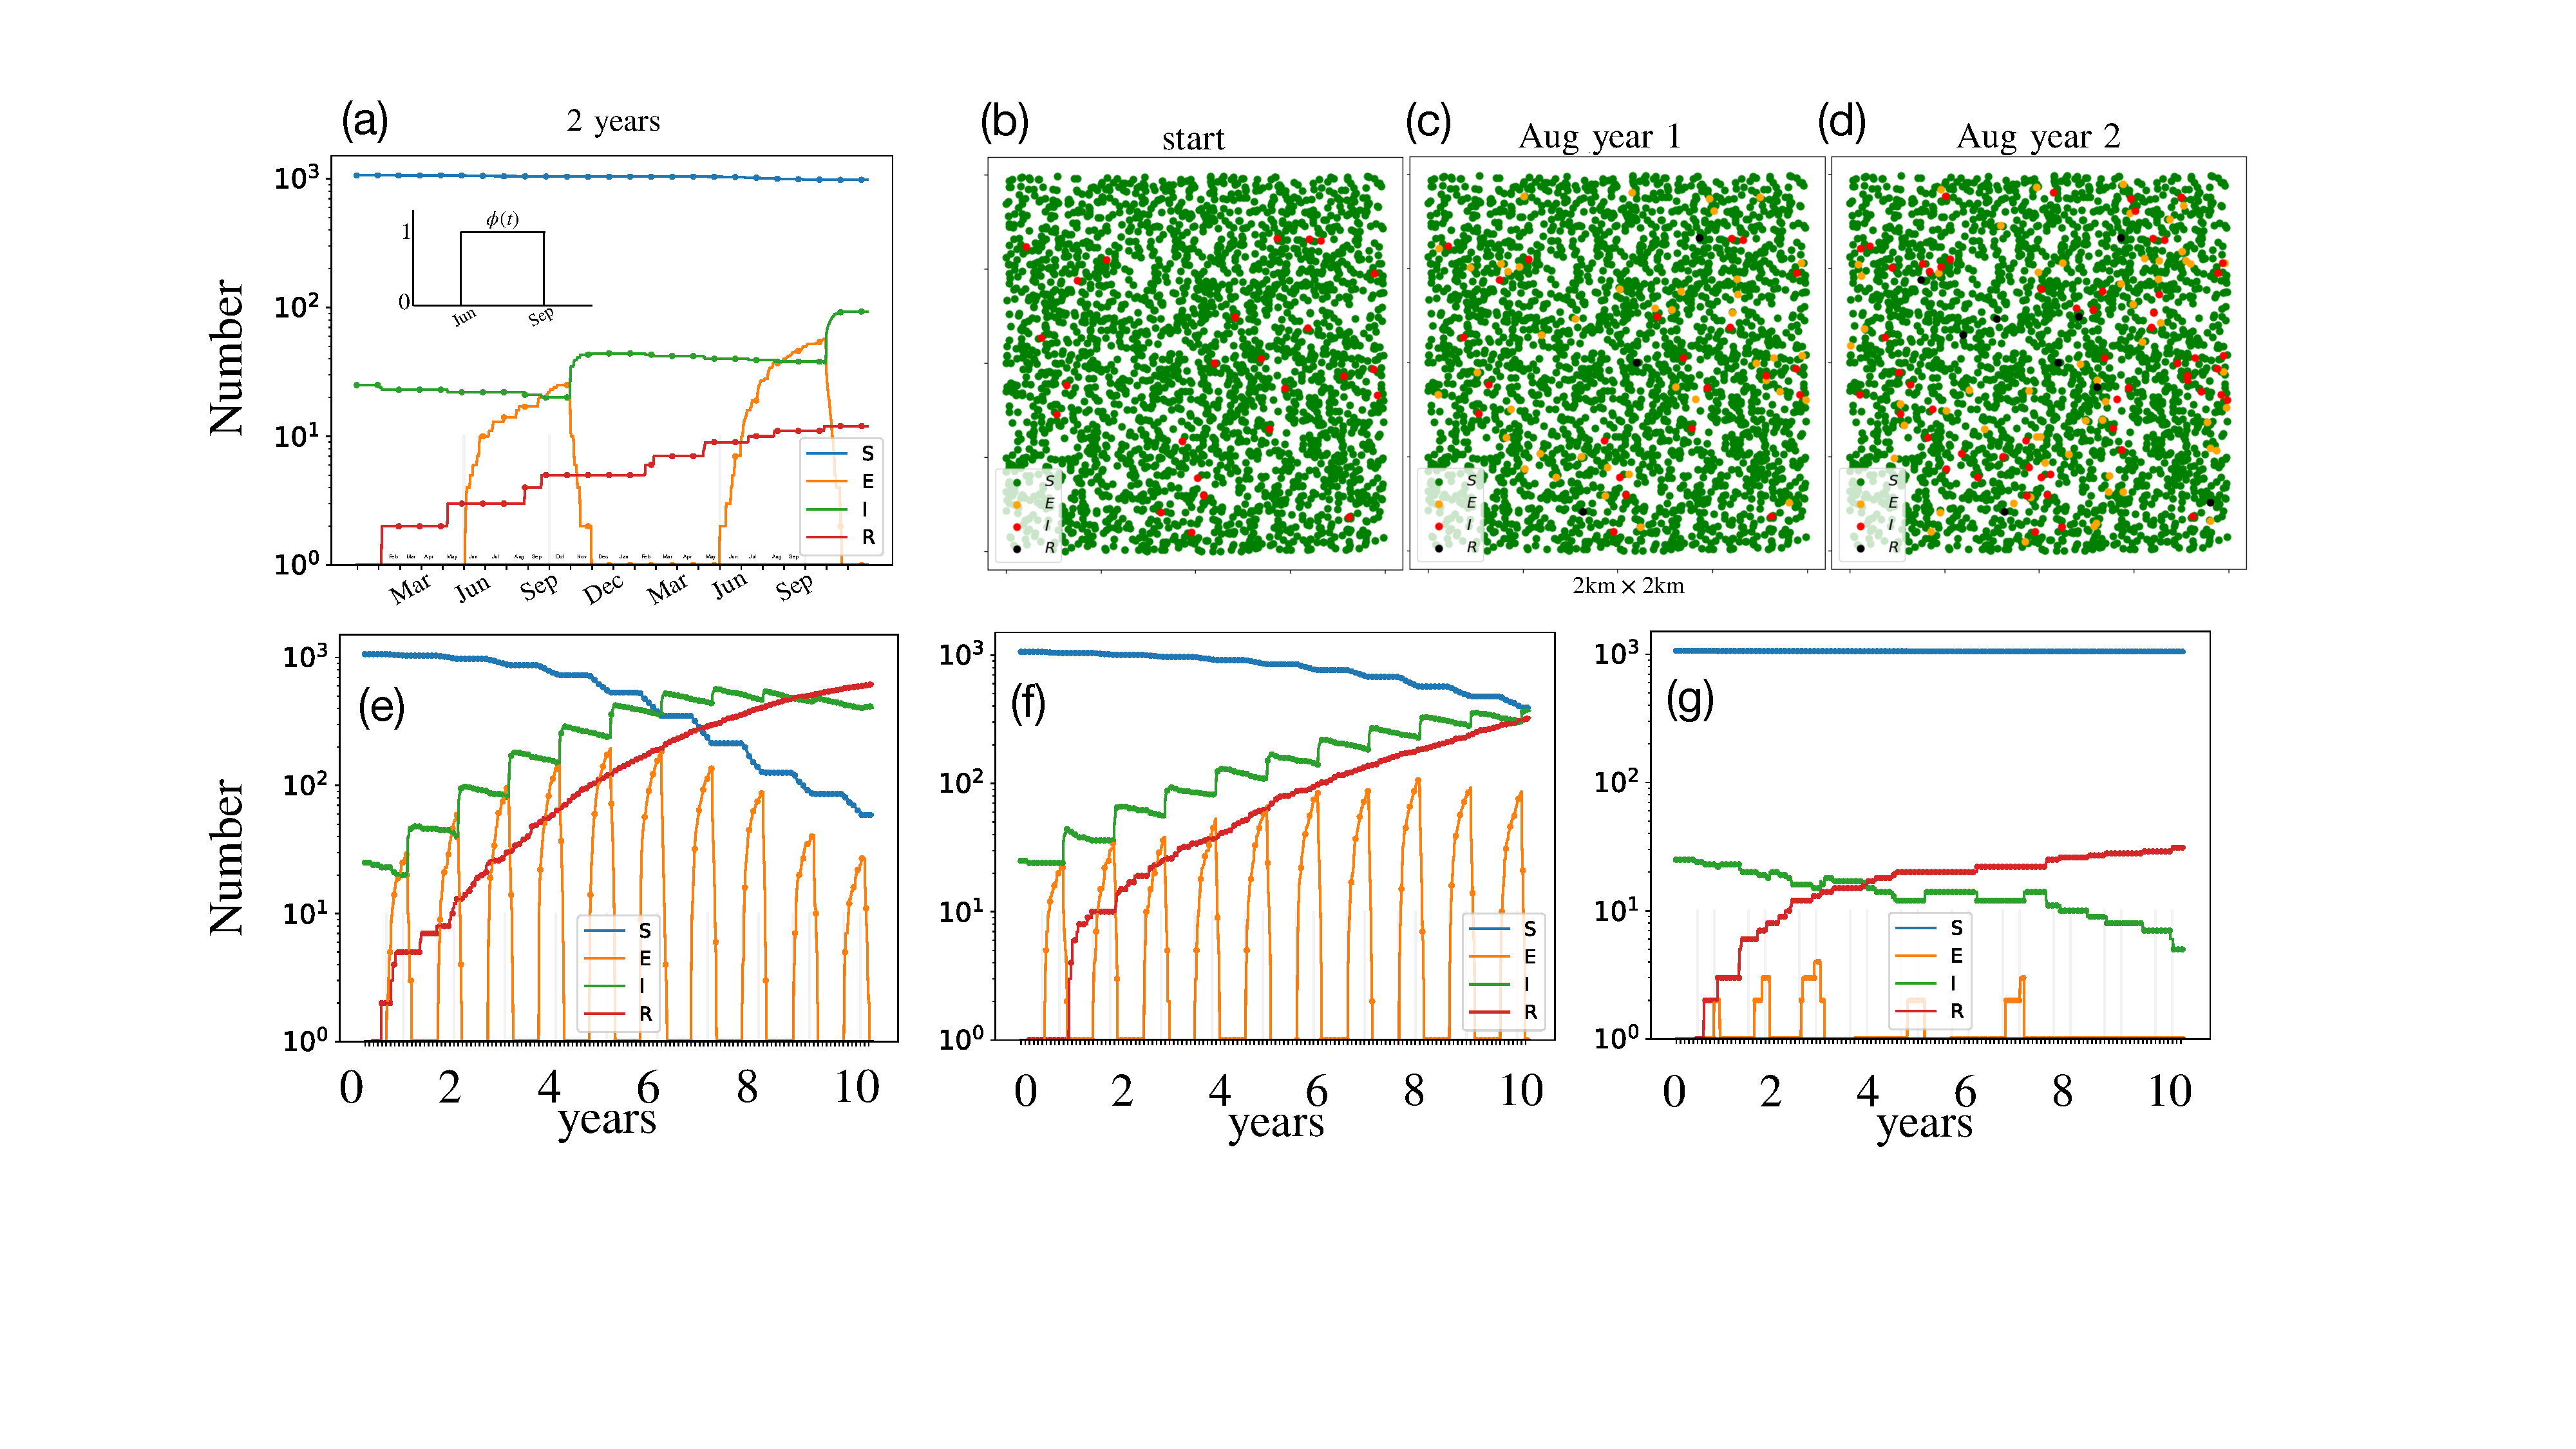
\includegraphics[scale=0.45]{chapter6/figures/fig4-seir.pdf} % SHOW 5 YEAR simulations instead, 10 years is too long...
     \caption{Simulating the $SEIR$ model over the median ash density, i.e. $\rho_{\mathrm{med}} = 0.011$. 
     In all panels, a small clump of $20$ infected hosts seeds the domain centre at time $t=0$.
     (a-b) The number of ash in each $SEIR$ compartment is plotted over five years for the model $\phi_1$-ga.
     Panels (a) and (b) depict simulations above ($\beta^*=2000$) and below ($\beta^*=500$) the epidemic threshold, respectively. 
     (c-f) The spatial progression of disease in a $2\mathrm{km} \times 2\mathrm{km}$ domain over a full year for model $\phi_1$-pl; 
     infectivity is fixed to  $\beta^*=3000$, well above the threshold.
     From the first sporulation season (c)-(d) to the second (e)-(f), secondary infections scatter throughout the whole domain, in contrast to the wave-like behaviour witnessed for small dispersal length scales in Chapter \ref{ch5:dispersal-model}.}
    \label{fig:SEIR-spread}
\end{figure}
\end{landscape}


\section{Seasonal $SEIR$ model behaviour}
\label{sec:seir-behaviour}

The essential $SEIR$ model behaviour is shown in Figure \ref{fig:SEIR-spread}, simulated with the median ash density in Great Britain\textemdash according to \cite{hill.data}.
For each year after the outbreak, a rise in the number of latently infected ash in $E$ can be seen during summertime sporulation, June-September, followed by a rise in the number of infectious ash in the autumn-winter. 
All model variants display the same pattern of seasonal behaviour. 

The number of ash in the $SEIR$ compartments is shown in Figure \ref{fig:SEIR-spread}(a-b) for two infectivity parameters in a $1\mathrm{km}\times1\mathrm{km}$ domain.
Figures \ref{fig:SEIR-spread}(a-b) depict two scenarios above and below the epidemic threshold for model $\phi_1$-ga;
the compartments are plotted over $5$ years with infectivity ($\beta^*$) parameters shown. 
In Figure \ref{fig:SEIR-spread}(a), the number of ash in $S$ decline, shown by the green line,
and during seasonal sporulation, large spikes in the number of latently infected ash can be seen in orange. 
Then, latently infected ash transition into $I$ during autumn and winter, as shown by the seasonal rise of $I$ in green.
For infectivity parameters below the epidemic threshold, Figure \ref{fig:SEIR-spread}(b), $S$ remains approximately constant as $I$ slowly declines. 
Interestingly, Figure \ref{fig:SEIR-spread}(b) demonstrates persistence in model of ADB; 
whereby, even if the epidemic parameters are below the threshold, the fungus may survive for long periods. 
In general, persistence in plant-based pathogens is one aspect that complicates epidemic control\textemdash see Chapter \ref{ch3:invasions_and_persistence} for a review of invasion and persistence in the spread of plant-based diseases.

The spatial progression of ADB in the $SEIR$ model is shown in Figures \ref{fig:SEIR-spread}(c-f) over a full year. 
The simulation in Figure \ref{fig:SEIR-spread}(c) begins with an initial condition of $20$ infected ash centrally distributed in the host landscape during March (not shown). 
At this point in the year, fungal fruiting bodies on infected leaf litter will be preparing to release ascospores.
During sporulation, secondary infections are produced, and latently infected ash spread throughout the domain, depicted by the orange dots in Figure \ref{fig:SEIR-spread}(c-d). 
At any time step, the chance of removal to the $R$ compartment s non-zero, demonstrated by the small number of black dots in Figures \ref{fig:SEIR-spread}(c-d).
After the sporulation season ends in September (not shown), latently infected ash begin to transition into the $I$ compartment;
eventually, all latently infect ash become infectious during the following season, reflected by the increased number of red dots in Figure \ref{fig:SEIR-spread}(e). 
The cycle will continue when the next cohort of secondary infections are produced in the following summer when the sporulation function next becomes non-zero.

\subsection{Sporulation: time-varying infectivity}
\label{ch6:sporulation}

Time varying infectivity rates are an important concept in epidemiology, this is true of epidemics in both human/animal \cite{svensson2007note, liu2012infectious} 
and botanical populations \cite{suffert2018some, leclerc2014estimating, time-varying-infectivity}.
In particular, ADB is known to have a seasonal life-cycle, and time-varying infectivity \cite{grosdidier2018tracking, hietala2013invasive}. 
The peak of ADB infectivity occurs during summertime sporulation when fruiting bodies on shed litterfall release ascospores.

To demonstrate robustness in the approach, two sporulation functions, $\phi_1(t)$ and $\phi_2(t)$, are used to model the time-dependent ADB ascospore production.
The choice of sporulation functions were inspired by the modelling work of \cite{time-varying-infectivity} and \cite{segarra2001epidemic}
(reviewed in Chapter \ref{ch2:lit-rev-compartmentalised-models}). 
Sporulation functions are described by step function and a normal distribution located at the midpoint between June and September:

\begin{equation}
\phi_1(t)  = \left\{
\begin{array}{ll}
      1 &  t \in [\mathrm{June,\ September}] \\
      0 & \mathrm{Otherwise} \\
\end{array} 
\right.
\end{equation}
and 
\begin{equation}
     \phi_2(t) =  \exp\big[-\frac{(t - T_{SP})^2}{2\sigma_{SP}^2}\big]
\end{equation}

\begin{figure}.
    \centering
    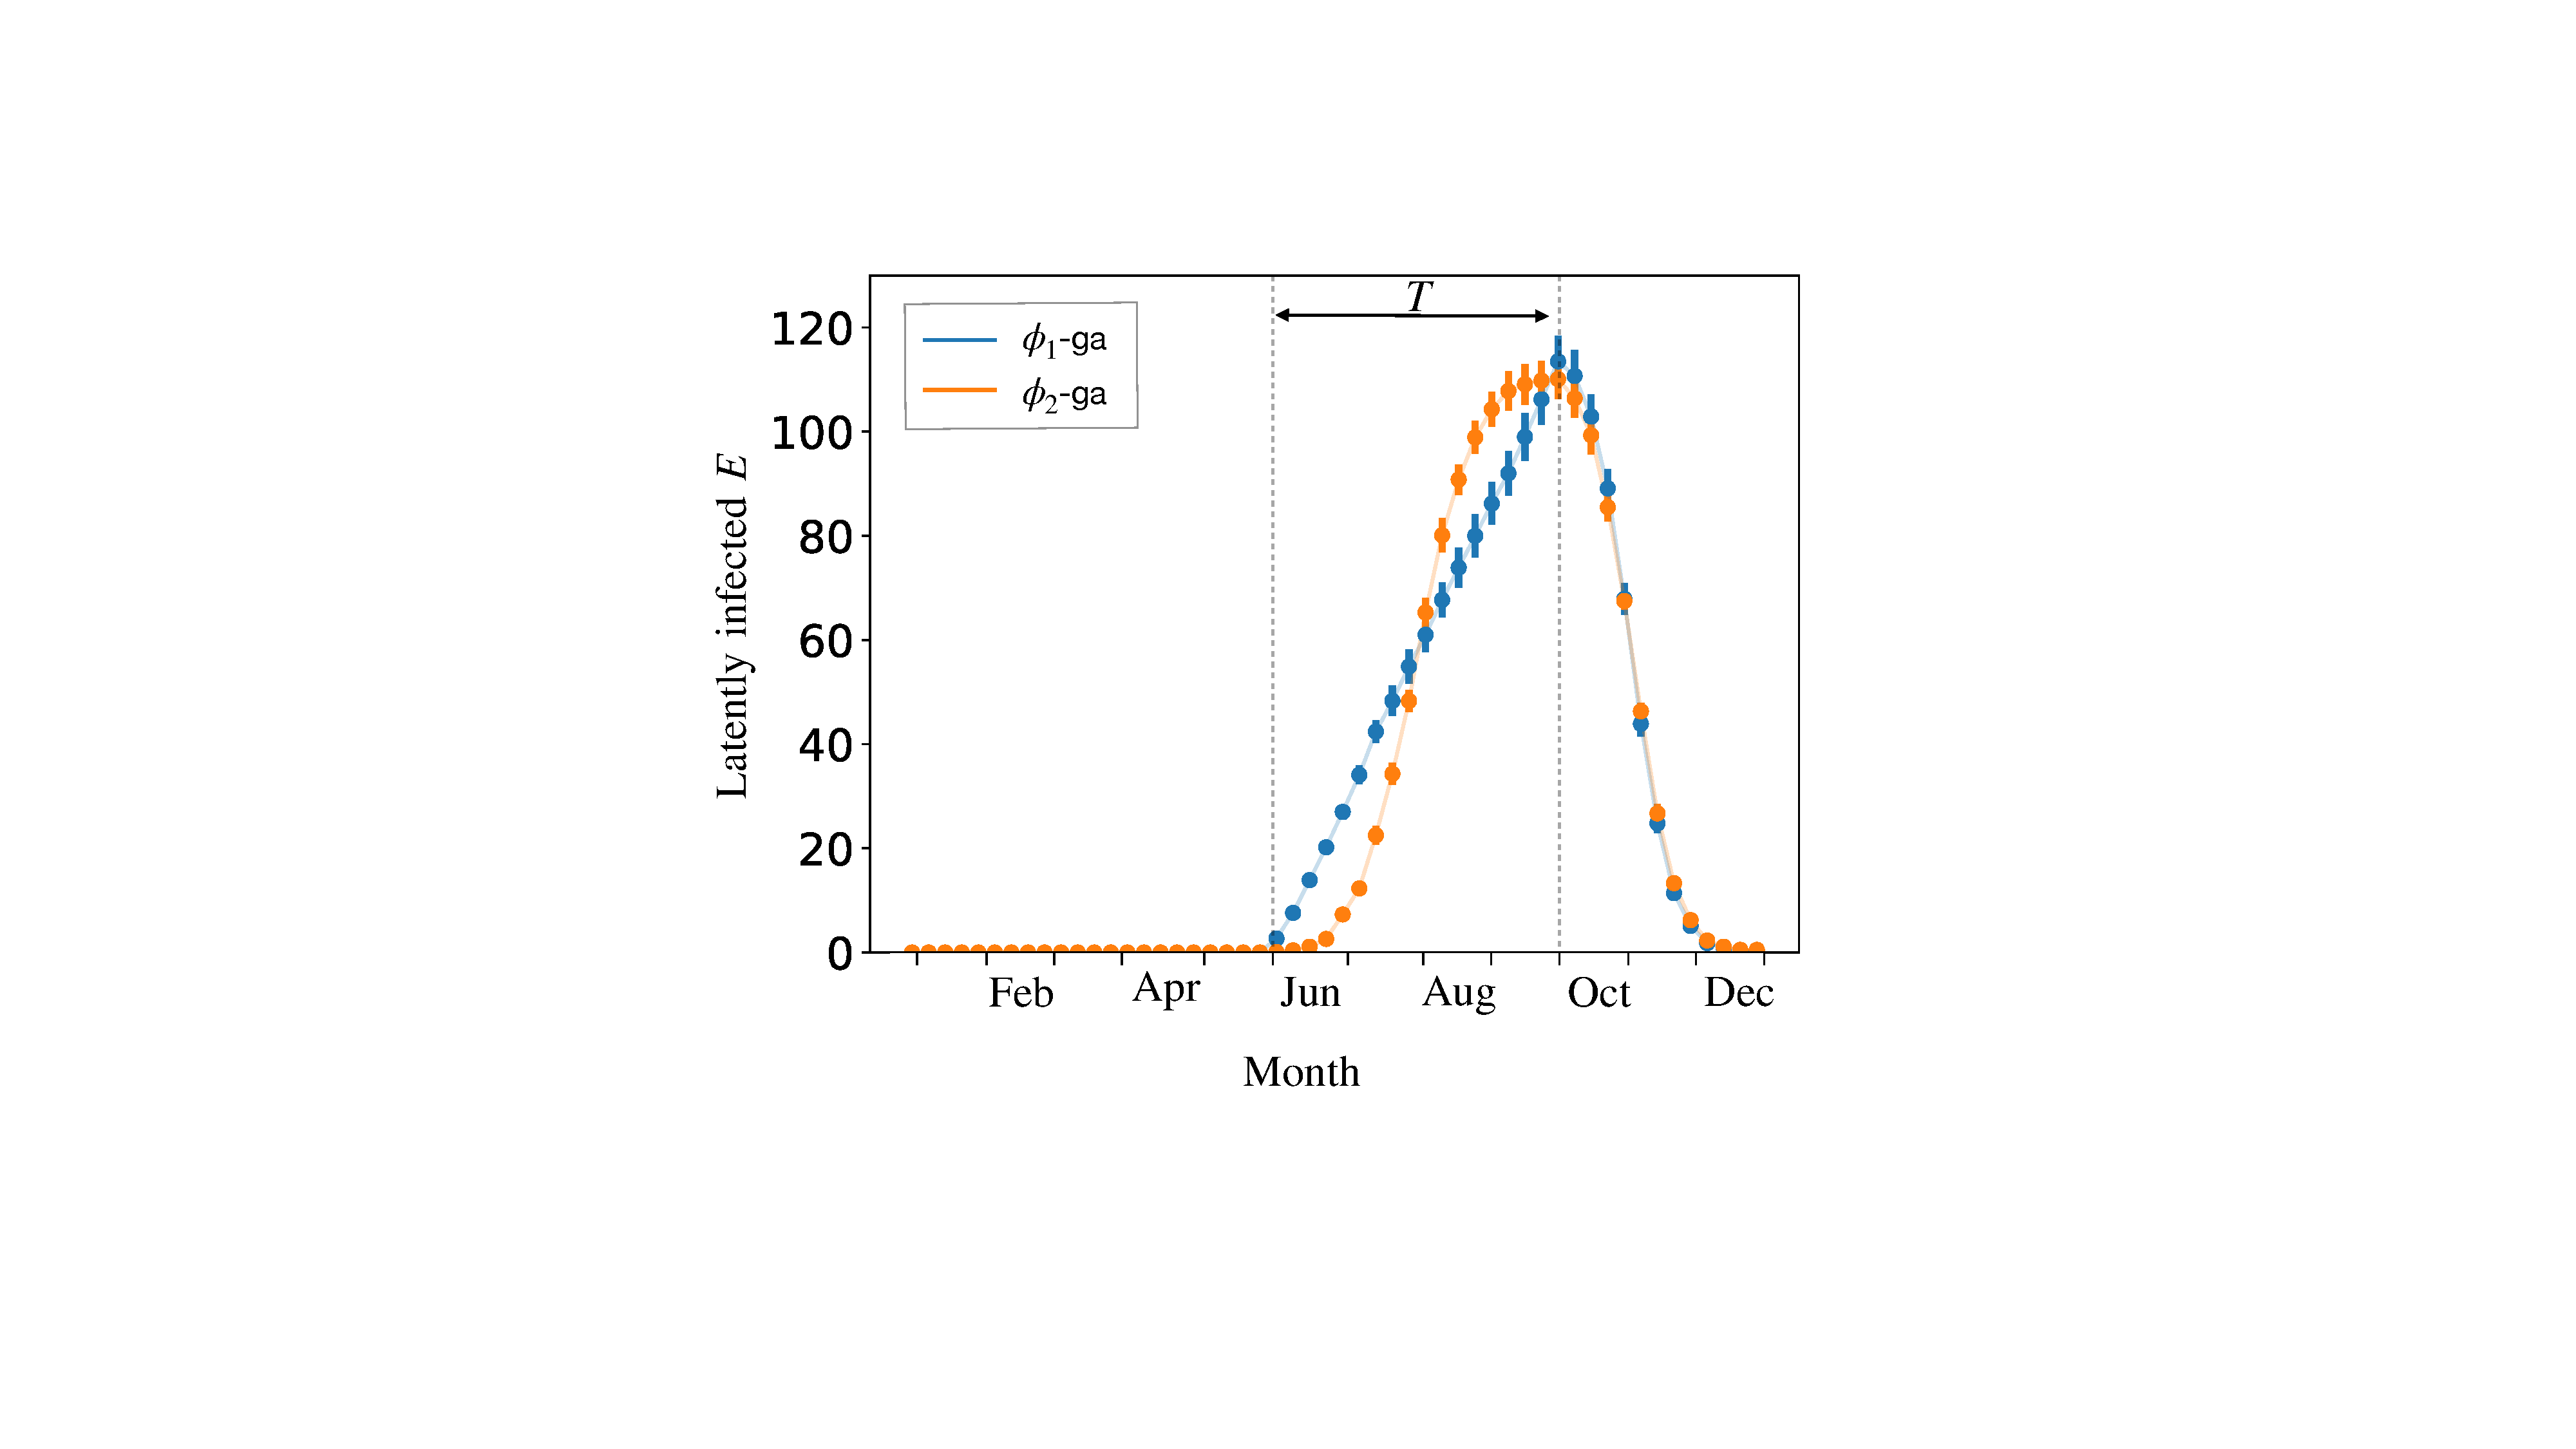
\includegraphics[scale=0.35]{chapter6/figures/fig5-sporulation.pdf}
    \caption{One year simulations contrasting the form of sporulation for models $\phi_1(t)$-ga and $\phi_2(t)$-ga, (a) and (b) respectively. 
    Both (a) and (b) depict the average number of infected trees that transition into the $E$ compartment over a single sporulation season; the standard error is shown by the error bars.
    An auxiliary infectivity, of value $\beta^*=2000$, effectively matches the epidemic impact between models\textemdash indicative of the area under each curve.}
    \label{fig:SEIR-sporulation}
\end{figure}

where $T_{SP}$ is taken to be the mid-point of June-September (i.e. late July/early August) and $\sigma_{SP}^2$ is a standard deviation of two weeks.
As discussed above, the choice of sporulation peak $T_{SP}$ and standard deviation $\sigma_{SP}$ together inform the earliest transitions $S\rightarrow E$ for $\phi_2$.
Due to the seasonality and perennial nature of ADB, both $\phi_1(t)$ and $\phi_2(t)$ repeat yearly, becoming non-zero during the months of June and September\footnote{Variations in ADB sporulation have been noted between European countries \cite{https://doi.org/10.1111/mpp.12073}, along with the potential for early-onset sporulation in the face of favourable environmental conditions. Although, the most generally agreed upon sporulation period is thought to be from June to September.}.
For $\phi_2$, the chance of new secondary infections outside of June-September is trivially small.

Figure \ref{fig:SEIR-sporulation} contrasts sporulation models by computing the number of ash transitioning into the $E$ compartment for one season over an ensemble of size $10$.
Simulations started with $100$ infected ash distributed randomly throughout a $\mathrm{5km \times 5km}$ domain at the mean GB ash density in January (i.e. time $t=0$ ).
Both models show a rise in the number of infected ash during the sporulation season.
The infectivity rate for function $\phi_2$ can be seen to vary, in contrast $\phi_1$ is uniform\textemdash both dispersal models $\phi_1$-pl and $\phi_2$-pl demonstrated the exact behaviour.
Although infectivity rates differed, the normalised infectivity $\beta^*$ ensured the same approximate area under each curve and, therefore, epidemic impact.

Both $\phi_1(t)$ and $\phi_2(t)$ aim to mirror the seasonal time-dependence of \textit{H. fraxineus} sexual reproduction.
In the seasonal $SEIR$ model, time-varying infectivity is achieved by multiplying the infectivity parameter with a sporulation function $\beta\phi(t)$.
In line with the parsimonious approach undertaken thus far, $\phi_1(t)$ and $\phi_2(t)$ are generic and aim to capture the essential dynamics of ADB spread.
However, a more complex model could aim to fit $\phi(t)$ to spore-trapping data, which could resemble a Gaussian-k function (e.g. see Figure 2. in \cite{grosdidier2018tracking}).
Although different sporulation models lead to the same effective behaviour (as discussed more below in section \ref{sec:tree-mortality}), 
non-uniform infectivity rates for ADB have a more robust basis in the literature \cite{grosdidier2018tracking, time-varying-infectivity, hietala2013invasive, segarra2001epidemic}.
So, the function $\phi_2$ can be considered more representative due to the non-uniformity and infectivity peak.

\subsection{Tree mortality}
\label{sec:tree-mortality}

Ash mortality due to ADB has been well-researched in different European countries, frequently over long-running 10-20 year experiments.
In this section, tree mortality is studied over long time scales to give insight into the scale of the epidemic, pathogen invasiveness and domain sensitivity.
However, host demography was neglected from the model, which is desirable for modelling the spread of pathogens targeting long-lived hosts \cite{doi:10.1098/rstb.1996.0059}.
Therefore, the long-running simulations presented in this section approximate the spread of ADB over considerable time scales to first-order.

\begin{figure}
    \centering
    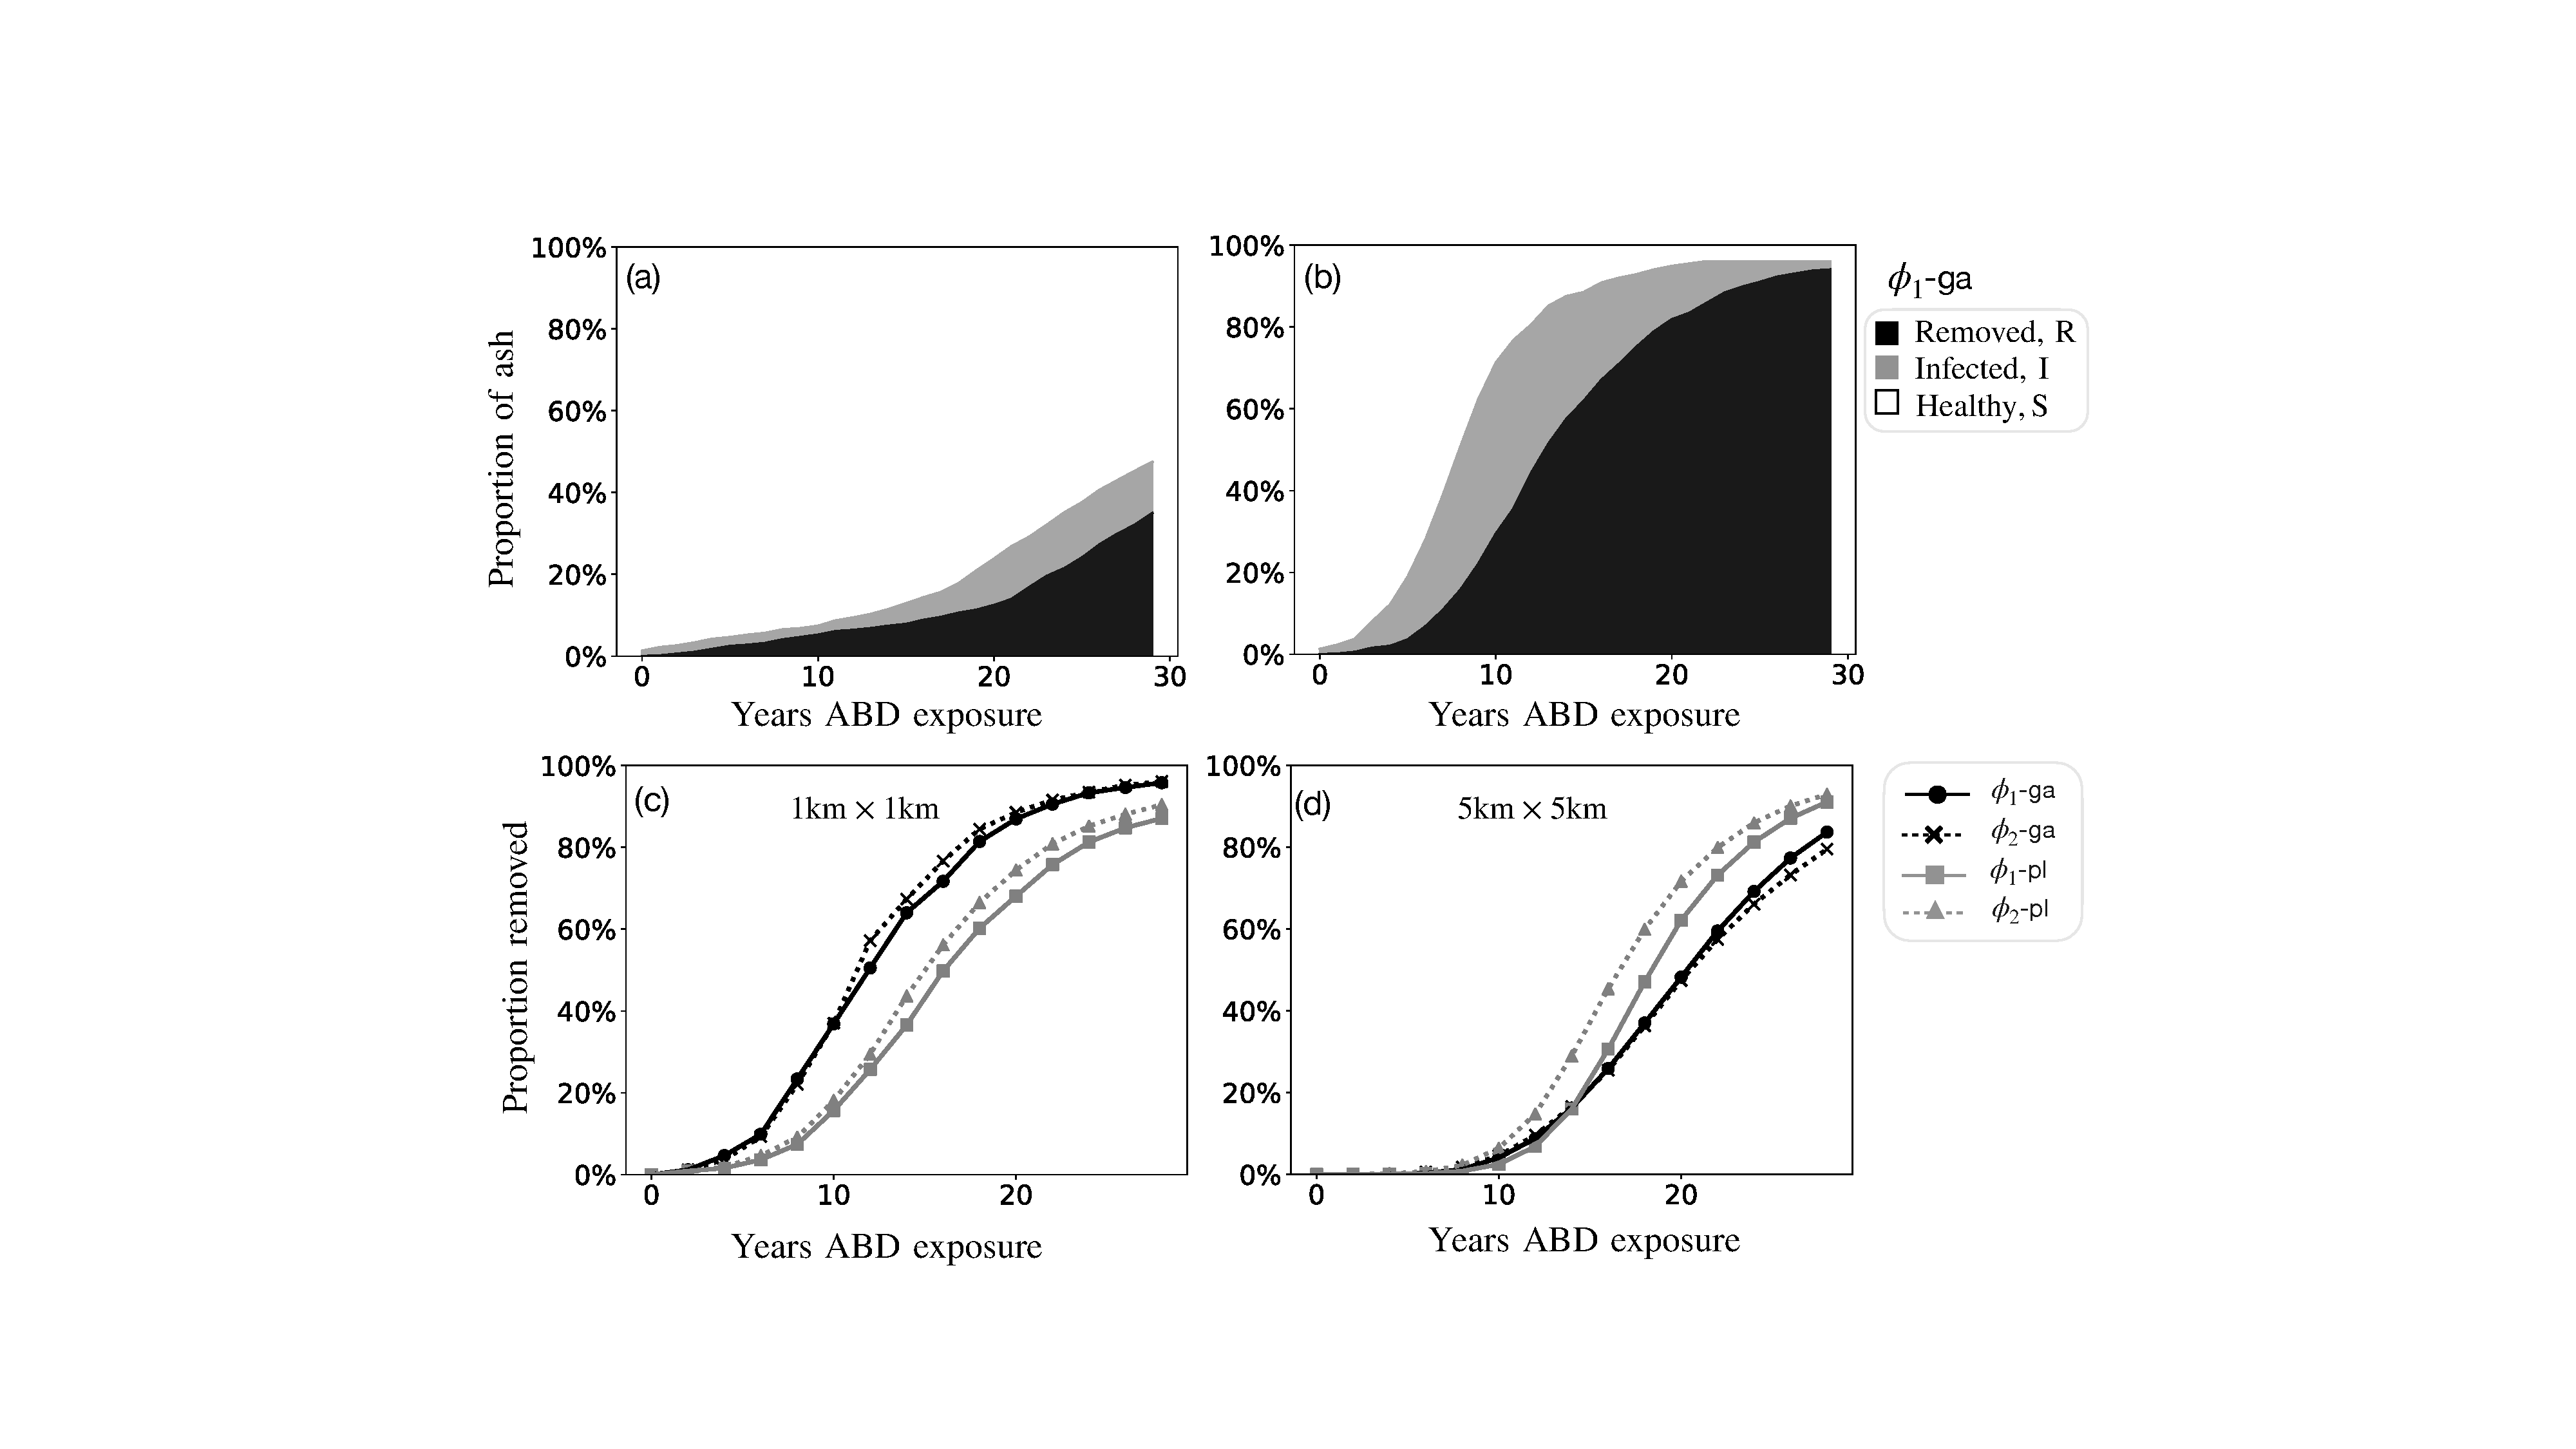
\includegraphics[scale=0.42]{chapter6/figures/fig6-mortality.pdf}
    \caption{Epidemic-scale in the $SEIR$ model, as measured by the proportion of ash in $S$, $I$ and $R$ (a-b) 
    The proportion of ash in $S$, $I$ and $R$ is shown over $30$ years of ADB exposure for $\phi_1$-ga. 
    Two different values of infectivity, $\beta^*=1000$ and $\beta^*=1500$, increase the proportion of trees in $I$ and $R$. 
    (c-d) The proportion of ash removed in all models after years of exposure with infectivity $\beta^*=1000$. 
    Differences between dispersal models are demonstrated by disparate epidemic-scales\textemdash indicated by the height between blue and orange curves.}
    \label{fig:ash-mortalty}
\end{figure}

Figures \ref{fig:ash-mortalty}(a-b) display the proportion of ash in $S$, $I$ and $R$ over $30$ years for the model $\phi_1$-ga with 
infectivity parameters $\beta^*=1000$ and $\beta^*=1500$, respectively. The simulations take place on a $1\mathrm{km}\times 1 \mathrm{km}$ domain, 
and both values of $\beta$ are above the threshold for an epidemic.
Initially, all simulations begin with a small number of infected ash at the domain centre.
As expected, the higher infectivity in Figure \ref{fig:ash-mortalty}(b) produces an outbreak that spreads through the domain much quicker.
Although, all systems in this framework above the epidemic threshold will, on average, reach $100\%$ mortality eventually.

The seasonal $SEIR$ model produced a characteristic sigmoidal s-shaped mortality curve for high mortality proportions 
(i.e. approaching $100\%$), shown in Figures \ref{fig:ash-mortalty}(b), this contrasts with the logistic ADB mortality 
curves presented by \cite{https://doi.org/10.1002/ppp3.11} that, on average, saturate to $\sim 60 \%$.
Other authors have witnessed similar s-shaped mortality curves, e.g. \cite{lohmus2014ash}.
Here, not including host demography precludes host-pathogen coexistence and prevents the $SEIR$ model from saturating below
$100\%$ mortality\textemdash as explained in more depth by \cite{time-varying-infectivity} in their manuscript.
Therefore, failing to reach a steady-state for long running simulations represents a limitation in the seasonal $SEIR$ model of ADB.

Figures \ref{fig:ash-mortalty}(c-d) show the mortality percentage on two different domain sizes for each model with a single infectivity parameter $\beta^*=2000$, well beyond the epidemic threshold.
For all models, the larger domain size effectively reduced the proportion of removed ash over the $30$ period because more trees populate the domain, shown in Figure \ref{fig:ash-mortalty}(c).
Figure \ref{fig:ash-mortalty}(c) confirms that on a smaller $1\mathrm{km}\times 1\mathrm{km}$ domain, the more localised Gaussian dispersal models give rise to a more significant epidemic impact.
This behaviour can be understood by noting that for inverse power law spread, secondary infections are on average likely to be under-counted
by virtue the of fat-tailed dispersal kernel extending beyond the domain boundary.
Increasing the domain size to $5\mathrm{km}\times 5\mathrm{km}$ brings both dispersal models into a closer agreement on the epidemic scale.
Nevertheless, directly comparing the epidemic scale between models is difficult considering the relationship between domain size and dispersal.

Domain size is known to play an integral role in shaping the evolution in spatially explicit population growth models \cite{tang2011asymptotic}.
A related topic, `plant-pathogen invasiveness and field-size', was investigated by \cite{mikaberidze2016invasiveness} in the context of crop disease.
In particular, \cite{mikaberidze2016invasiveness} demonstrated that $R_0$ saturates to a maximum for a suitably large domain size, beyond which increasing the domain size had no effect on $R_0$.
Therefore, choosing a suitable domain size for each dispersal mode remains critical to capture the epidemic scale accurately.
In the next section, a definition of $R_0$ is outlined for the seasonal $SEIR$ model, and we revisit the topic domain size.

\section{Defining an $R_0$}
\label{sec:SEIR-R0-definition}
% Although it is hard to enforce a true $R_0$ value, the most important feature introduced from the definition is a threshold from which we can see if a local invasion is likely to take place.

Before properly investigating the $SEIR$ model, the pathogens' ability to invade must be defined. 
Tree mortality, shown in Figure \ref{fig:ash-mortalty}, gives insight into the final-size epidemic and the time-scale of spread.
However, computing tree mortality requires long simulation run-times spanning years which is problematic given that host-demography is not included in the model.
Moreover, as we look to scale up the $SEIR$ model over large areas within GB, running tree mortality simulations over long periods
becomes increasingly computationally expensive. 

Consequently, the basic reproduction number will be employed to navigate these computational challenges. 
As we saw previously, through sections \ref{sec:spatially-explicit-reproduction-ration}-\ref{sec:contract-traced-R0}, 
the system can be characterised by a basic reproduction ($R_0$) number that corresponds to a threshold, above which epidemic severity drastically increases.

\textit{From this point on, unless otherwise stated, the method for calculating $R_0$ is based on the average number of secondary infections
resulting from the first-generation of infected hosts, as per definition \ref{def:R0_contact_traced}. However, we assume here that secondary infections
characterise the transition $S\rightarrow E$, and the number of first-generation secondary infections $(R_0^{(1)})$ is measured over the mean lifetime
of infected ash, i.e. five years. The first-generation contact-traced secondary infections $R_0^{(1)}$ will be denoted by $R_0$ for brevity.}

% Within this epidemic system, secondary infections are mediated by dispersal with a spatially structured host population.
% Chapter \ref{ch5:dispersal-model} explored the use of a spatially-explicit $R_0$ as a function of various epidemiological parameters; however, a proper investigation into $R_0$ and the domain size was omitted\footnote{As referred to here, $L$ represents the domain size, i.e. the boundaries/area over which an epidemic may spread. The scaling constant between pixels, $\alpha=5\mathrm{m}$, remains fixed for each simulation.}.
% To this aim, the contact-traced $R_0$ is studied over domain-size to explain the results of Figures \ref{fig:ash-mortalty}(c-d).

\subsection{Computing $R_0$: initial conditions}

\label{section:initial-conditions}

This section will investigate initial conditions for just $\phi_1$-ga and $\phi_2$-pl, 
as differences between sporulation models were negligible.
Initial conditions play a role in shaping the final value of $R_0$ and produce distinct model behaviours. 
At $t=0$, the following initial conditions can seed the domain:  
IC1) infected hosts occupy the domain centre  
IC2) infected hosts are scattered randomly throughout the domain.
Figure \ref{fig:seir-ash-IC} contrasts the contact-traced $R_0$ for 
first-generation infected ash over five years between the models $\phi_1$-ga and $\phi_2$-pl.
Although the ensemble average $\overline{R}_0$ (i.e. the horizontal black line) compared similarly 
for each initial condition, differences can be seen in the statistics.

Figure \ref{fig:seir-ash-IC} shows an ensemble of $R_0$ values for IC1 (a) and IC2 (b) with 10 and 20 initially infected 
ash with epidemic parameters well above the threshold\footnote{
Following the findings of Chapter \ref{ch5:dispersal-model}, a small number of initially infected trees seed 
the domain at $t=0$; having more than one infected tree helps to reduce initial stochasticity, 
which thereby lowers the number of early pathogen extinction events.}.
A more localised dispersal kernel in $\phi_1$-ga produces a value of $R_0$ that is generally higher for IC2 and lower for IC1.
Adjacently infected hosts at $t=0$ reduce the density of susceptible ash within a relatively small 
neighbourhood\textemdash up to a maximum radius of approximately $\approx 3\ell_{ga}$.
When several infected trees are located nearby, as for IC1, $R_0$ is generally smaller because the
surrounding neighbourhood quickly becomes saturated with infected trees, limiting the number of new secondary infections.
The effect of $R_0$-saturation for model $\phi_1$-ga is most apparent in Figure \ref{fig:seir-ash-IC}(a) 
when a lower value of $\overline{R}_0$ results by increasing the number of infected ash to 20.

\begin{figure}
    \centering
    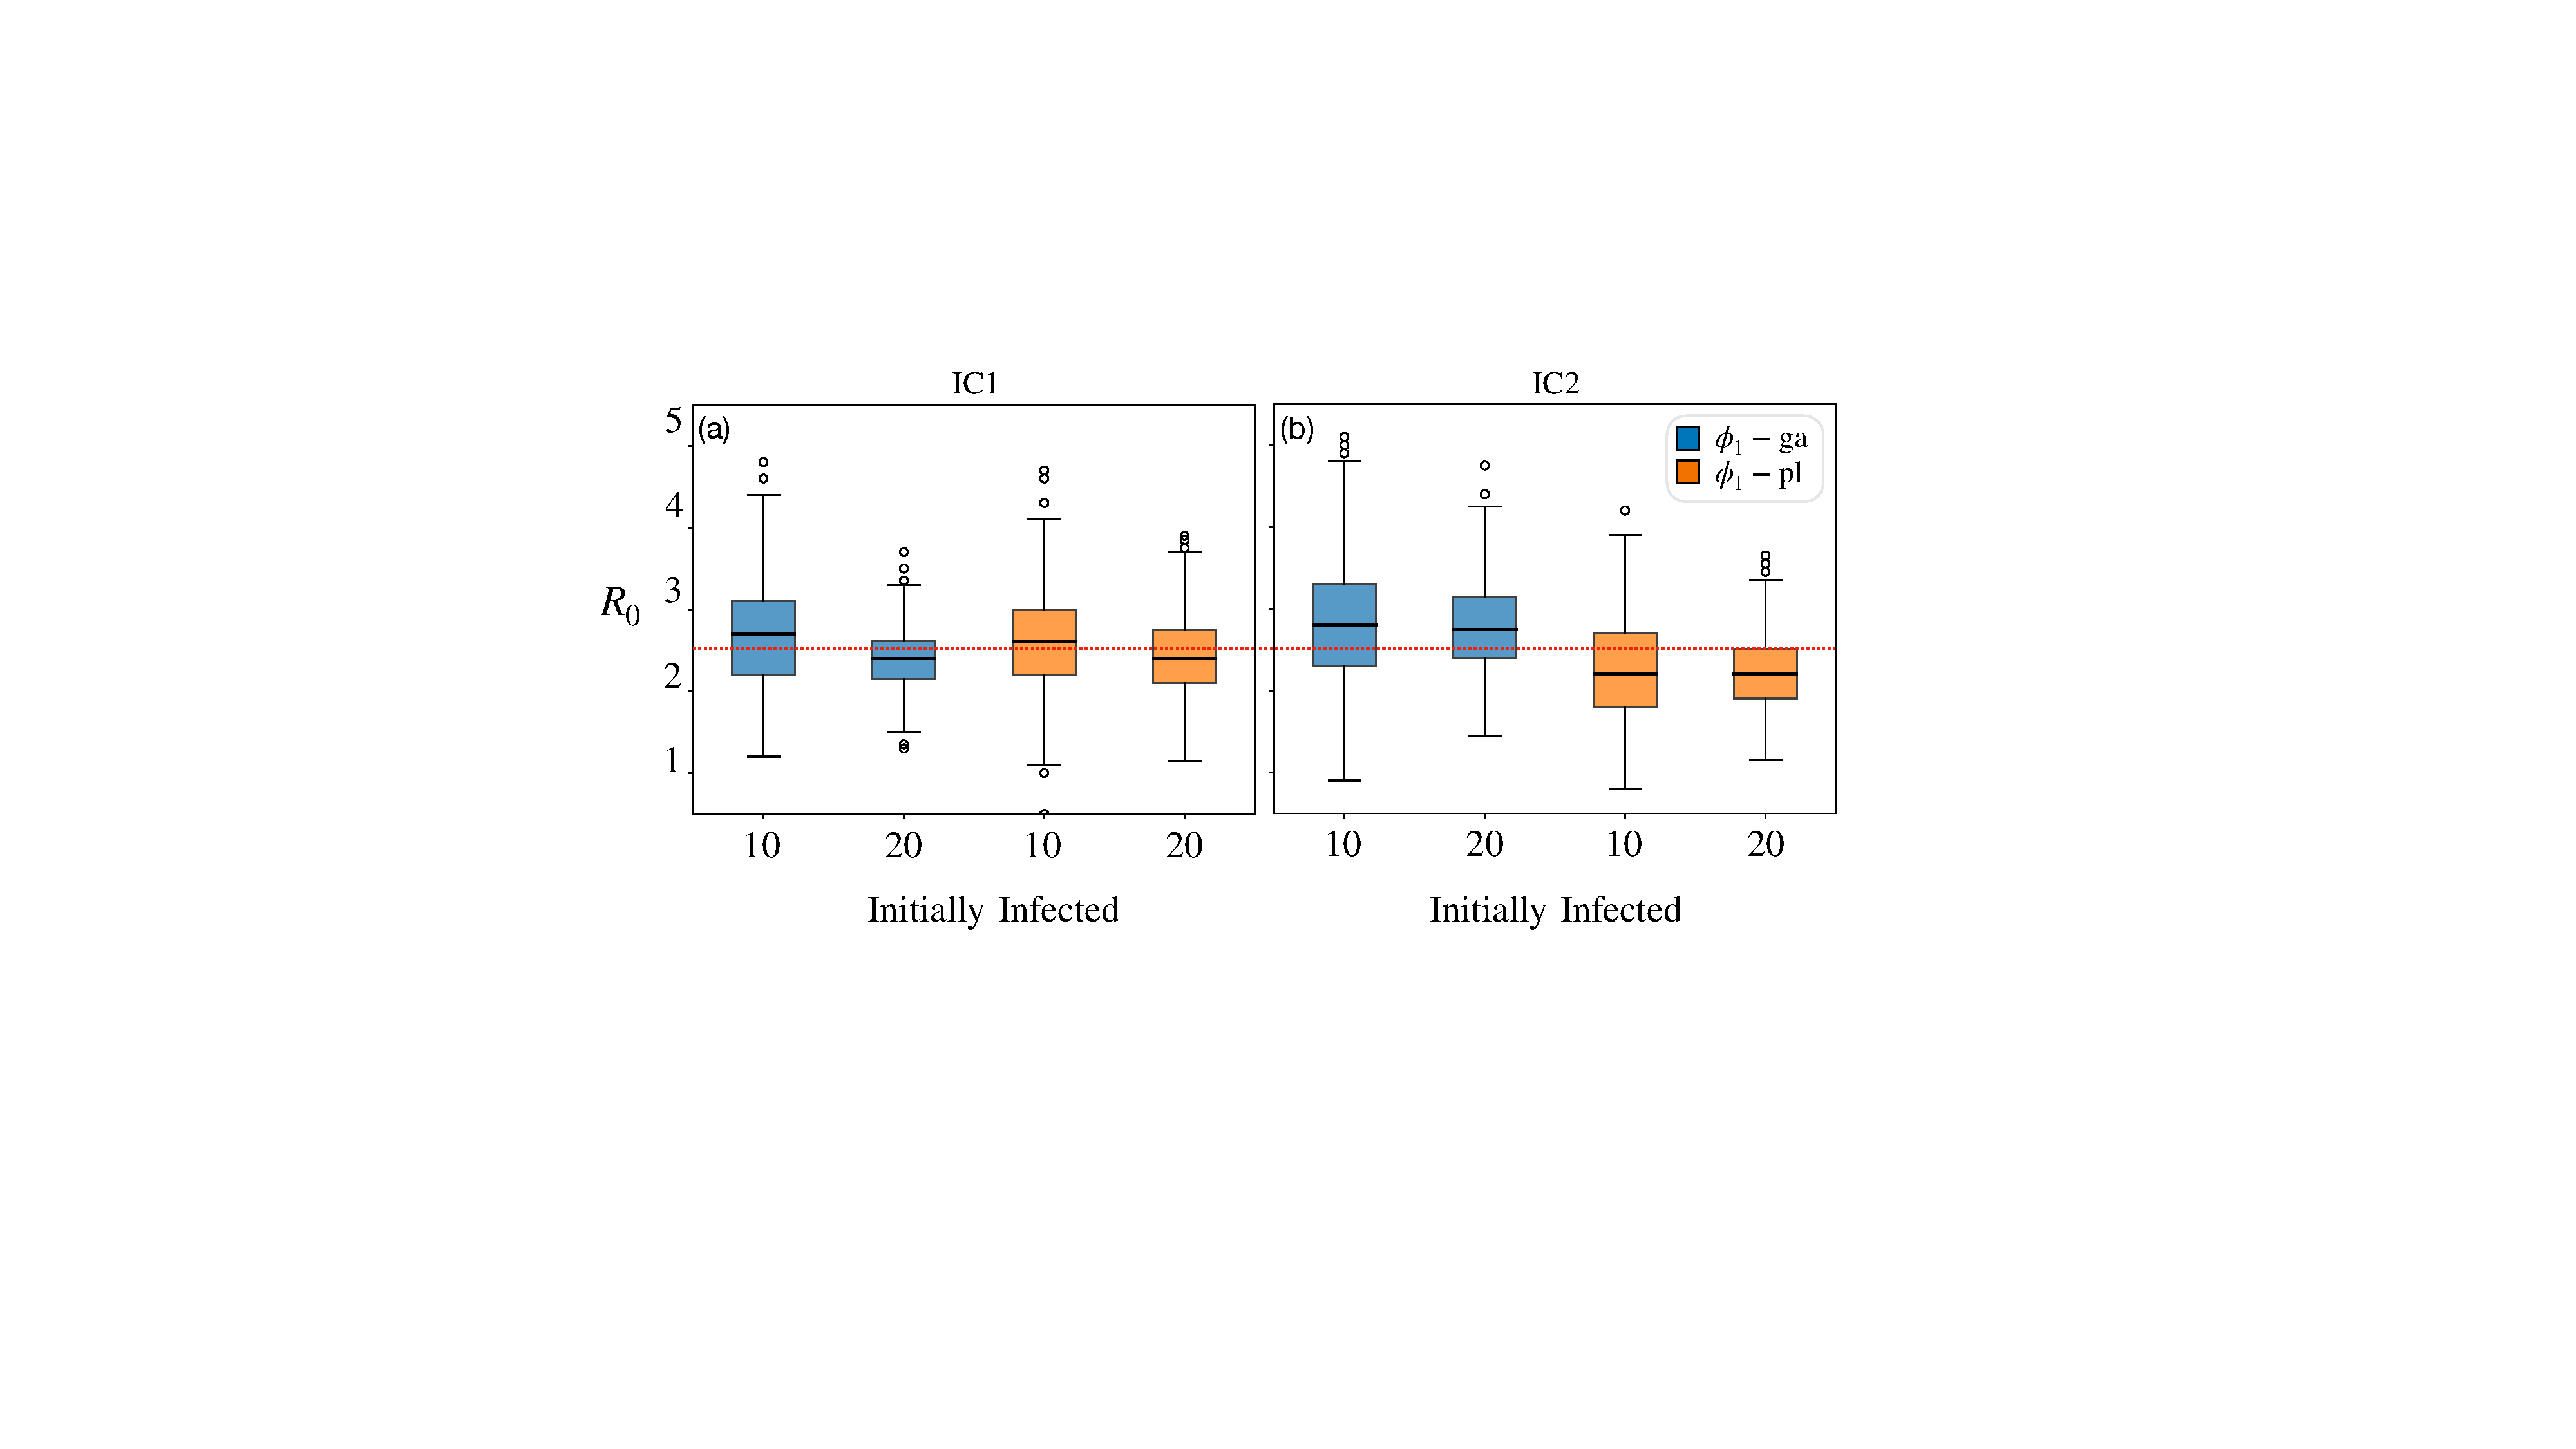
\includegraphics[scale=0.475]{chapter6/figures/fig5-IC.pdf}
    \caption{
    The effect of four different initial conditions on $R_0$ are compared for the Gaussian and inverse power law models, $\phi$-ga and $\phi$-pl.
    Each box describes $R_0$ simulated over an ensemble of size $N=500$. 
    (a) At $t=0$, between 10 and 20 infected hosts are placed at the domain centre for $\phi$-ga (in blue) and $\phi$-pl (in orange).
    (b) At $t=0$, between 10 and 20 infected hosts are randomly scattered throughout the domain for both models.
    The mean value of $R_0$ compares most similarly using IC1.
    Epidemic parameters for each ensemble: $\beta^*=1500$, $\rho_{avg}=0.017$, on a domain of size $\mathrm{2km\times 2km}$.
  }
    \label{fig:seir-ash-IC}
\end{figure}

In contrast, initial conditions had the opposite effect on inverse power law based epidemics.
For inverse power law spread, Figure \ref{fig:seir-ash-IC}(a-b) demonstrate that $R_0$ is generally lower for IC2 and higher for IC1.
Fat-tailed dispersal models show a higher sensitivity to the domain boundary.
In particular, domain-sensitivity is demonstrated in \ref{fig:seir-ash-IC}(b), where more infected hosts are located closer to the domain edge.
These observations can be explained by realising that fat-tailed dispersal kernels are more likely to extend beyond the boundary.
Therefore, for the same normalised value of $\beta^*$, inverse power law models are more likely to undercount $R_0$ locally if measured inside a smaller domain.
Notwithstanding, secondary infections induced by $\phi_1$-pl spread over a wider area, and the effect of $R_0$-saturation is far less than $\phi_1$-ga.

Overall, $\overline{R}_0$ agreed closely between models when infected ash are placed at the domain centre IC1\textemdash indicated by distance of $\overline{R}_0$ about the red horizontal line.
Moreover, boundary effects and domain sensitivity was the least when using IC1.
Ensemble simulations of $R_0$ are thus chosen to evolve from the domain centre going forward.
Even though, for IC1, the epidemic impact is slightly lowered for Gaussian-based spread, on account of $R_0$-saturation.
This points more towards a difference in model behaviour rather than artefacts of domain boundary size.


\subsection{Domain size $L$ and $R_0$}
\label{sec:r0-vs-L}

Before the small-scale $SEIR$ model of ADB can be spatially scaled up over GB, a suitable spatial and temporal 
scale must be chosen to measure $R_0$. The purpose of this section is to compute $R_0$ over different sized 
domains from IC1, i.e. a small number of infected trees located at the domain centre at $t=0$.
Choosing a sufficient domain length ($L$) is desirable to accurately capture pathogen invasiveness within each model.
Following the arguments laid out in section \ref{sec:I-to-R}, $R_0$ values are determined over the mean 
lifetime of infectious ash, i.e. $\lambda=5\mathrm{yr}$. According to their exponentially distributed lifetimes, 
infected ash can survive for more extended periods, although this accounts for a decreasingly small  the host population.

As remarked earlier, studies have shown that $R_0$ for crop disease can depend on the field size \cite{mikaberidze2016invasiveness} 
and saturates for a sufficiently large field. Here, we have a similar scenario: $R_0$ should be computed inside a sufficiently large domain,
such that further domain size increases yield the same value of $R_0$ for repeated simulations. In contrast, running simulations inside a smaller domain will 
underestimate the reproductive ratio, and consequently, overall epidemic impact \cite{R0-perc-ref, time-varying-infectivity}.

Figure \ref{fig:r0-domain-size} reveals how both dispersal models relate to the domain-size.
By counting the number of secondary infections that result from the first-generation of infected ash (at $t=0$), we can plot a distribution revealing how far away infections are likely to be produced.
Figures \ref{fig:r0-domain-size}(a-b) show the number of secondary infections induced a distance $D$ away from each infected source over $500$ repeated simulations.
Distributions for three different domain sizes are shown in Figure \ref{fig:r0-domain-size}(a-b).

Unsurprisingly, Figure \ref{fig:r0-domain-size}(a) and (b) reflect the Gaussian and inverse-power law dispersal kernels. 
However, Figure \ref{fig:r0-domain-size}(a-b) also show that secondary infections are unlikely to occur near first-generation infected ash.
A low secondary infection count close to infectious sources reflect the average space between hosts, set by $\rho$.
A higher density host distribution increases the relative proportion of induced secondary infections close to the source $<0.1\mathrm{km}$.

\begin{figure}
    \centering
    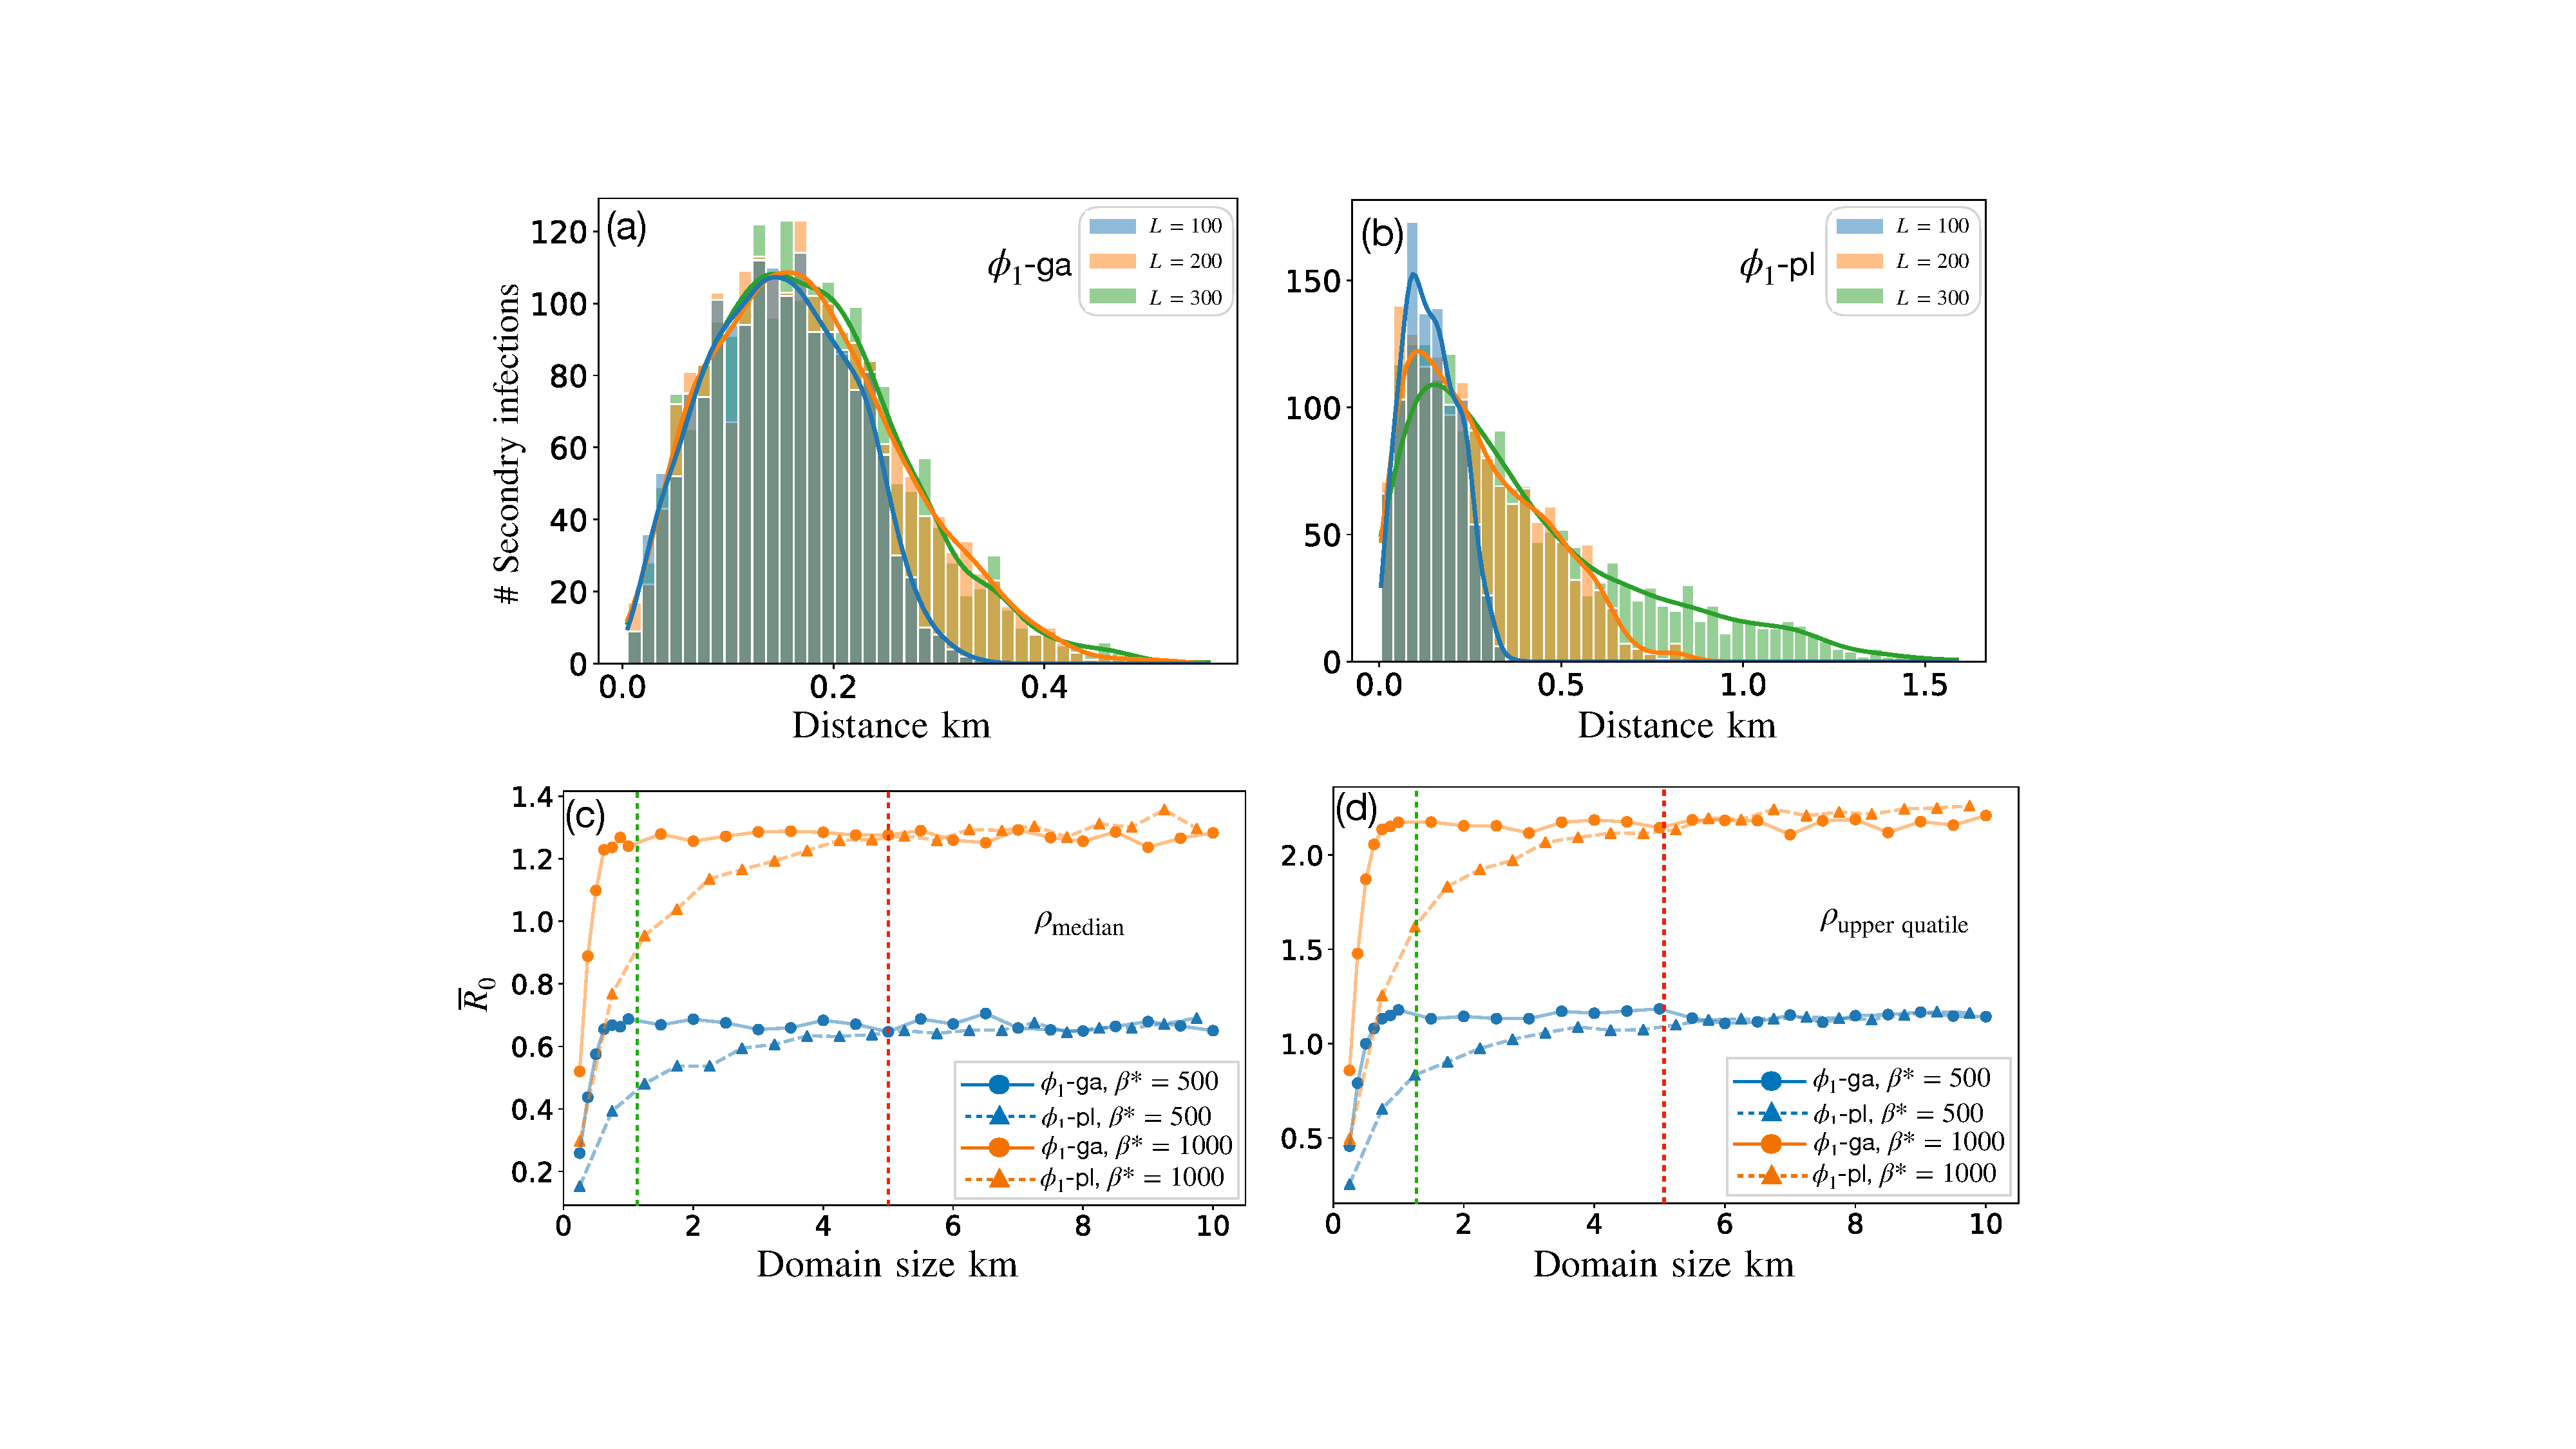
\includegraphics[scale=0.42]{chapter6/figures/fig5-R0-domain-size.pdf}
    \caption{The relationship between $R_0$ and the domain length, $L$. 
    For all panels, simulations run over five years or until the pathogen becomes extinct, whichever comes first.
    (a-b) Distributions show the number of secondary infections induced by distance over an ensemble of $500$ repeats for Gaussian and inverse power law dispersal kernels.
    Secondary infections are computed inside three different domain lengths of $L \in [100, 200, 300]$ (i.e. $\mathrm{500m\times500m,\ 1km\times1km,\ 1.5km\times1.5km}$) for epidemic parameters above threshold, $\beta^*=1000$ and $\rho_{avg} = 0.017$. Inverse power law spread demonstrates a higher domain sensitivity due to the fat-tailed kernel extending beyond the domain edge. (c-d) An ensemble-averaged reproductive ratio $\overline{R}_0$ is computed from $500$ repeated simulations over different domain lengths, up to a maximum of $L=2000$ or $\mathrm{10km \times 10km}$. The value of $\overline{R}_0$ is gauged at the median and upper quartiles of ash tree densities, (c) and (d), respectively, and at two infectivities shown in blue and orange. The value of $R_0$ saturates at around $\mathrm{1km\times1km}$ for Gaussian-based dispersal kernels and $\mathrm{5km\times5 km}$ for inverse power law dispersal kernels.}
    
    \label{fig:r0-domain-size}
\end{figure}

From Figure \ref{fig:r0-domain-size}(a-b) becomes visually apparent why domain sensitivity varies between dispersal models.
In Figure \ref{fig:r0-domain-size}(a), the number of infections is reduced for Gaussian dispersal at $L=100$, indicated by the smaller distribution tail in blue.
Although, increasing the domain length to $L=300$ produced no observable difference to $L=200$.
In all Gaussian simulations, no secondary infections were witnessed beyond $0.6\mathrm{km}$, in line with the results from \cite{grosdidier2018tracking}. 
On the other hand, a small number of secondary infections in the model $\phi_1$-pl can be seen up to the domain edge $1.5\mathrm{km}$ away.
Thus, if the domain size is below a minimum value of $L$, epidemics that observe inverse power law dispersal will be lowered due to an under-estimated total number of secondary infections.
For the exact value of $\beta^*$, $\phi_1$-pl can be seen to travel much further than $\phi_1$-ga and echos the difficulty of controlling fat-tailed pathogen dispersal \cite{WEBIDEMICS}, and more broadly, LDD.

Figures \ref{fig:r0-domain-size}(c-d) show how the mean value of $\overline{R}_0$ for each dispersal model saturates for a critical value of $L$, 
for two domains at the median and upper quartile of ash density $\rho_{med}=0.011$ and $\rho_{uq}=0.019$ (a) and (b) respectively.
Simulations for two infectivity parameters $\beta^* \in [500, 1000]$ are shown in blue and orange.
The computed value of $\overline{R}_0$ shows the aforementioned characteristic increase, up to a maximum saturation value.
Each infectivity and tree density combination produced a similar saturation point of $L \approx 1\mathrm{km}$ for $\phi_1$-ga and $L\approx 5\mathrm{km}$ for $\phi_1$-pl, the vertical green and red lines, respectively. 

From Figures \ref{fig:r0-domain-size}(c-d), a suitable domain length $L$ can be ascertained for each dispersal model, 
found to be $\mathrm{1km\times1km}$ for models $\phi_1$-ga and $\phi_2$-ga, and $\mathrm{5km\times5km}$ for models $\phi_1$-pl and $\phi_2$-pl. 
Moving onward, a proper characterisation of the GB ash tree canopy cover data set produced by \cite{hill.data} will be conducted,
before we determine $R_0$ as a function of host density in section \ref{section:r0-tree-density}.

\section{Constructing $R_0$-maps over Great Britain}

\label{sec:r0-map-construct}
In this section, $R_0$ values of the small-scale $SEIR$ model of ADB will be projected onto the host distribution of ash, 
given by \cite{hill.data}, to create landscape-level $R_0$-maps over Great Britain. 
Doing so will permit the investigation of a novel control strategy in Chapter \ref{ch7:landscape-level-control} 
and allow the local-scale epidemic severity, based on tree-to-tree interactions, to be efficiently scaled over large areas.

\subsection{Ash host distribution}

\begin{figure}
    \centering
    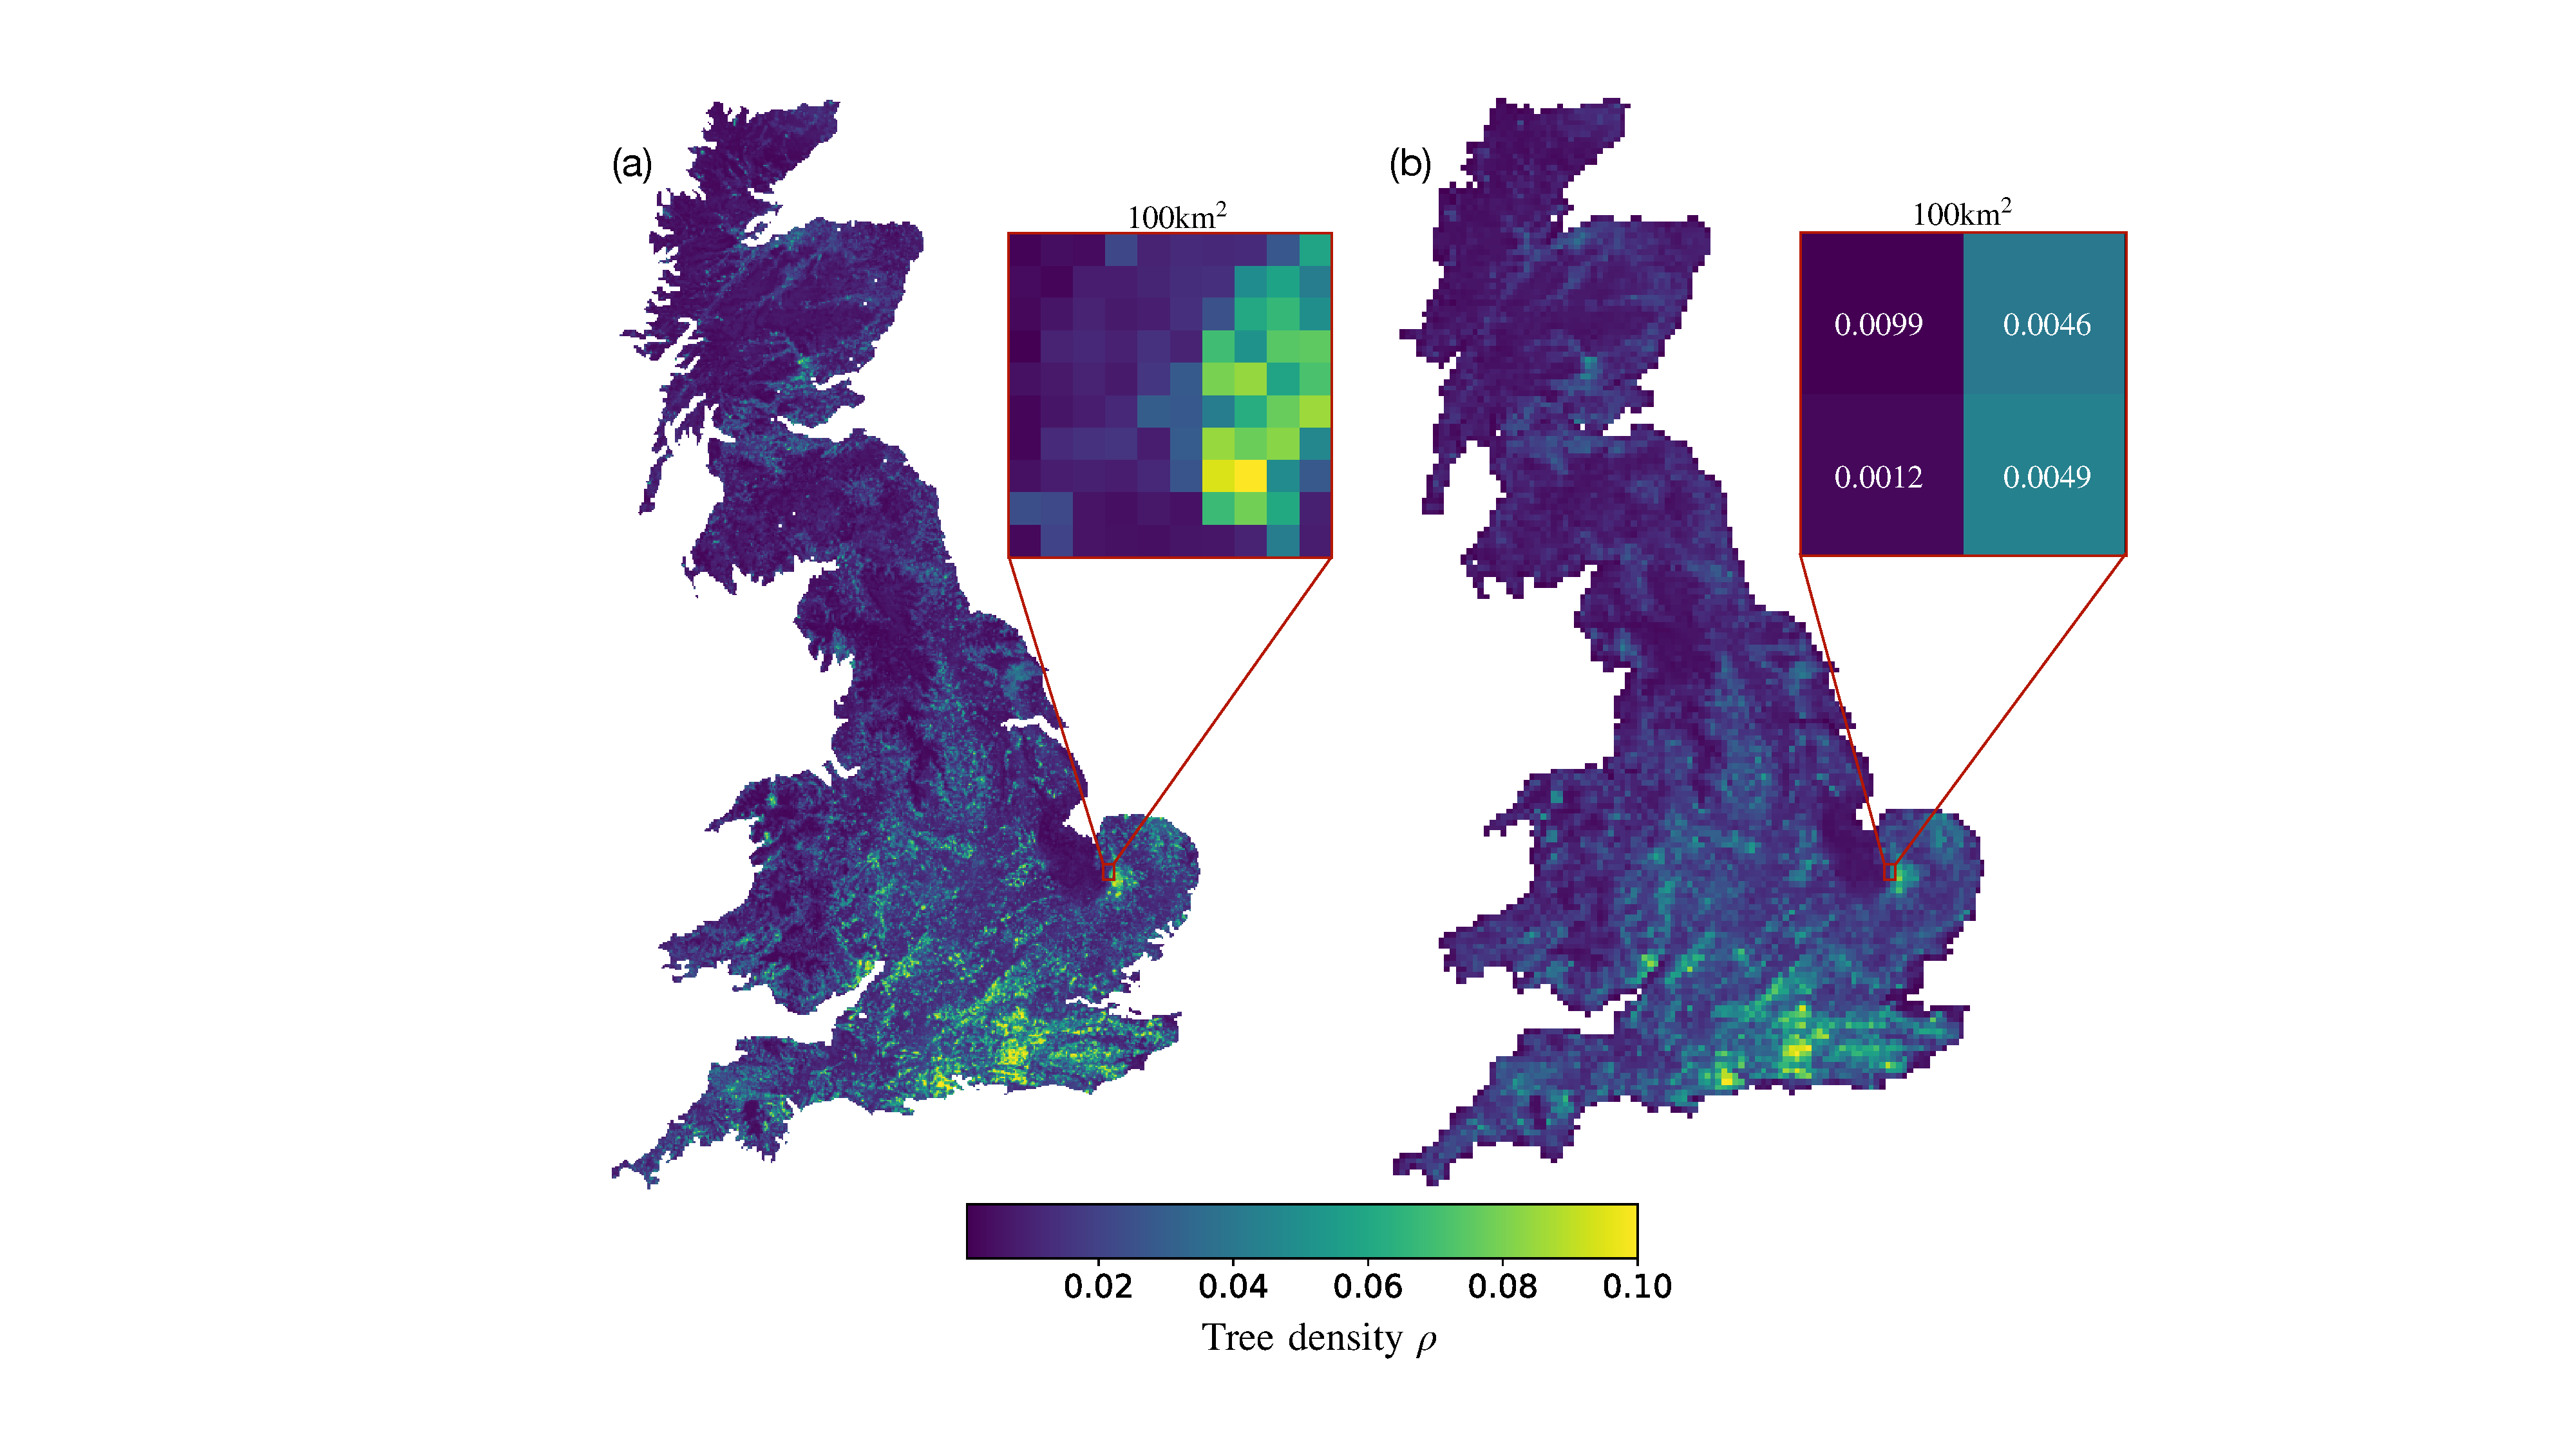
\includegraphics[scale=0.45]{chapter6/figures/fig-ash-data.pdf}
    \caption{The ash canopy cover data, as modelled by \cite{hill.data}, is converted into a map of tree density. (a) A map of ash densities at the original resolution of $1\mathrm{km} \times 1\mathrm{km}$, the inset consisting of $10\times 10$ pixels (b) A coarse-grained map of ash densities at a resolution of $5\mathrm{km} \times 5\mathrm{km}$, the inset consists of $2 \times 2$ pixels. Both insets show the same $100\mathrm{km^2}$ area, and illustrates how coarse-graining the host distribution results in a loss of spatial structure. A small number of densities over $10\%$ were excluded from the density-map.}
    \label{fig:ash-host-data}
\end{figure}

Ash densities were parameterised by ash the abundance data provided by \cite{hill.data}. 
Previously, the oak canopy cover dataset given by \cite{hill.data} was used previously in Chapter \ref{fig:ch4_uk_spread} 
alongside a toy model of landscape-level tree disease. The canopy cover datasets produced by \cite{hill.data} combine
several data sources that partly cover Great Britain, regression methods then extrapolate canopy cover over the whole of Great Britain.
Conveniently, ash happened to be among the most accurate data sets given by \cite{hill.data}. 
For a more in-depth description of the methods used by \cite{hill.data} and a review of host data in general, see Chapter \ref{ch2:hostdata}.

The modelled ash canopy cover data had to undergo minor modifications to complement the $SEIR$ model. 
Firstly, the raw abundance values were re-scaled into a dimensionless tree density $\rho$. 
The exact process was outlined in Chapter \ref{ch5:dispersal-model}, i.e. by converting the units $\mathrm{ha/km^2}$ to kilometre-squared
of ash cover per kilometre-squared of land. Secondly, the domain resolution has to be re-scaled to reflect the spatial scale of local 
wind-borne dispersal, as parameterised by \cite{grosdidier2018tracking}. 
Lastly, the small number of patches with exceedingly high densities were capped to $\rho_{max} = 0.10$, thus forming a hard upper limit in the density map.

Figure \ref{fig:ash-host-data}(a) shows a density map of ash, at the original resolution of
$\mathrm{1km}\times \mathrm{1km}$, produced from abundance data given by \cite{hill.data}.
The inset shows a block of $10\times10$ pixels, each of size $1\mathrm{km} \times 1 \mathrm{km}$.
In the small-scale Gaussian dispersal-based $SEIR$ model, a domain size of $\mathrm{1km}\times \mathrm{1km}$ was shown sufficient
to measure the average $R_0$ over a five-year period\textemdash demonstrated by Figures \ref{fig:r0-domain-size}(c-d).
However, the inverse power law models required a larger domain size of $\mathrm{5km}\times \mathrm{5km}$ to prevent underestimating epidemic severity.
Figure \ref{fig:ash-host-data}(b) shows the host distribution coarse-grained to a resolution of $\mathrm{5km}\times \mathrm{5km}$ pixels.
The insets of Figures \ref{fig:ash-host-data}(a-b) compare the same region.
Although, in Figure \ref{fig:ash-host-data}(b), pixels are effectively averaged and coarse-grained to larger $5\mathrm{km} \times 5 \mathrm{km}$ patches.
The resulting domain is smoother and therefore losses spatial structure.

From Figures \ref{fig:ash-host-data}(a-b), the south of England contains the highest concentration of high-density ash patches, 
and ash become progressively less abundant in Scotland and coastal locations, in western Wales, for example. 
A higher density of ash can be expected to yield a higher number of secondary infections, 
in line with the results of section \ref{ch3:two-param-model} and Chapter \ref{ch5:dispersal-model}.

\subsection{Tree density and $R_0$}
\label{section:r0-tree-density}

% - \cite{severns2019consequences}: R0 70, highly dense white stripe rust, 

Figures \ref{fig:R0-map-generation}(a-c) illustrated the relationship between $R_0$ and ash density.
Figure \ref{fig:R0-map-generation}(a) shows a PDF (probability density function) of ash densities $\rho$ over the map of Great Britain\textemdash overlaid with a KDE shown in red.
As noted above, few locations support densities of $\rho=0.10$ and over\footnote{
The original $\mathrm{1km \times 1km}$ map resolution contained $2.2\times 10^4$ $1\mathrm{km^2}$ data points, 
with some outlier pixels having densities in the interval $\rho \in [0.10, 0.30]$ which were excluded from the analysis due to 
A) the increased computational run-time required to simulate the $SEIR$ model of ADB  
and B) densities beyond $0.10$ account for a negligible portion of the overall population.}. 
Between the limits of $\rho \in [10^{-2}, 10^{-1}]$, the PDF follows a power law of the form $\sim \rho ^{-k}$, as evident from linearity in the logarithmic inset axes.
The distribution had a fitted exponent of $k=1.90$, shown by the black line.

Figures \ref{fig:R0-map-generation}(b-c) contrast the behaviour between $R_0$ and tree density $\rho$ for linear and peaked sporulation functions, $\phi_1$ and $\phi_2$ respectively.
Values of $R_0$ were ensemble-averaged over $100$ repeated simulations.
For the two values of infectivity, $\beta^*\in [500, 1000]$ shown, all model variants display the same linearity between $R_0$ and $\rho$ \textemdash also explored in Chapter \ref{ch5:dispersal-model}.
The dashed orange and blue lines show how high values of $\beta$ and $\rho$ result in a considerable value of $R_0$.
For high $R_0$ values, the Gaussian dispersal models $\phi_1$-ga and $\phi_2$-ga begin to deviate from linearity as density is increased,
due to the phenomena of $R_0$-saturation witnessed in section \ref{section:initial-conditions}.
Figure \ref{fig:R0-map-generation}(b) reveals a larger area of shaded grey, 
suggesting that the sole difference between sporulation models is that $\phi_2$-ga deviates from linearity more than $\phi_1$-ga.

In Figures \ref{fig:R0-map-generation}(b-c), the regime of pathogen extinction is indicated by the horizontal red lines, 
which correspond to a critical `density threshold' denoted by $\rho_c$ (equivalent to the threshold $R_0 = 1$).
When used in conjunction with the data-set from \cite{hill.data}, Figures \ref{fig:R0-map-generation}(b-c) represent an appropriate projection of $R_0$ over the map of Great Britain.
Below the threshold $R_0=1$, infected ash can still survive and reproduce (i.e. persist below the threshold, as we saw in Figure \ref{fig:SEIR-spread}(c)), albeit at slower rates.
Negating below-threshold patches is a vital assumption\textemdash discussed more below.

\begin{landscape}
\begin{figure}
    \centering
    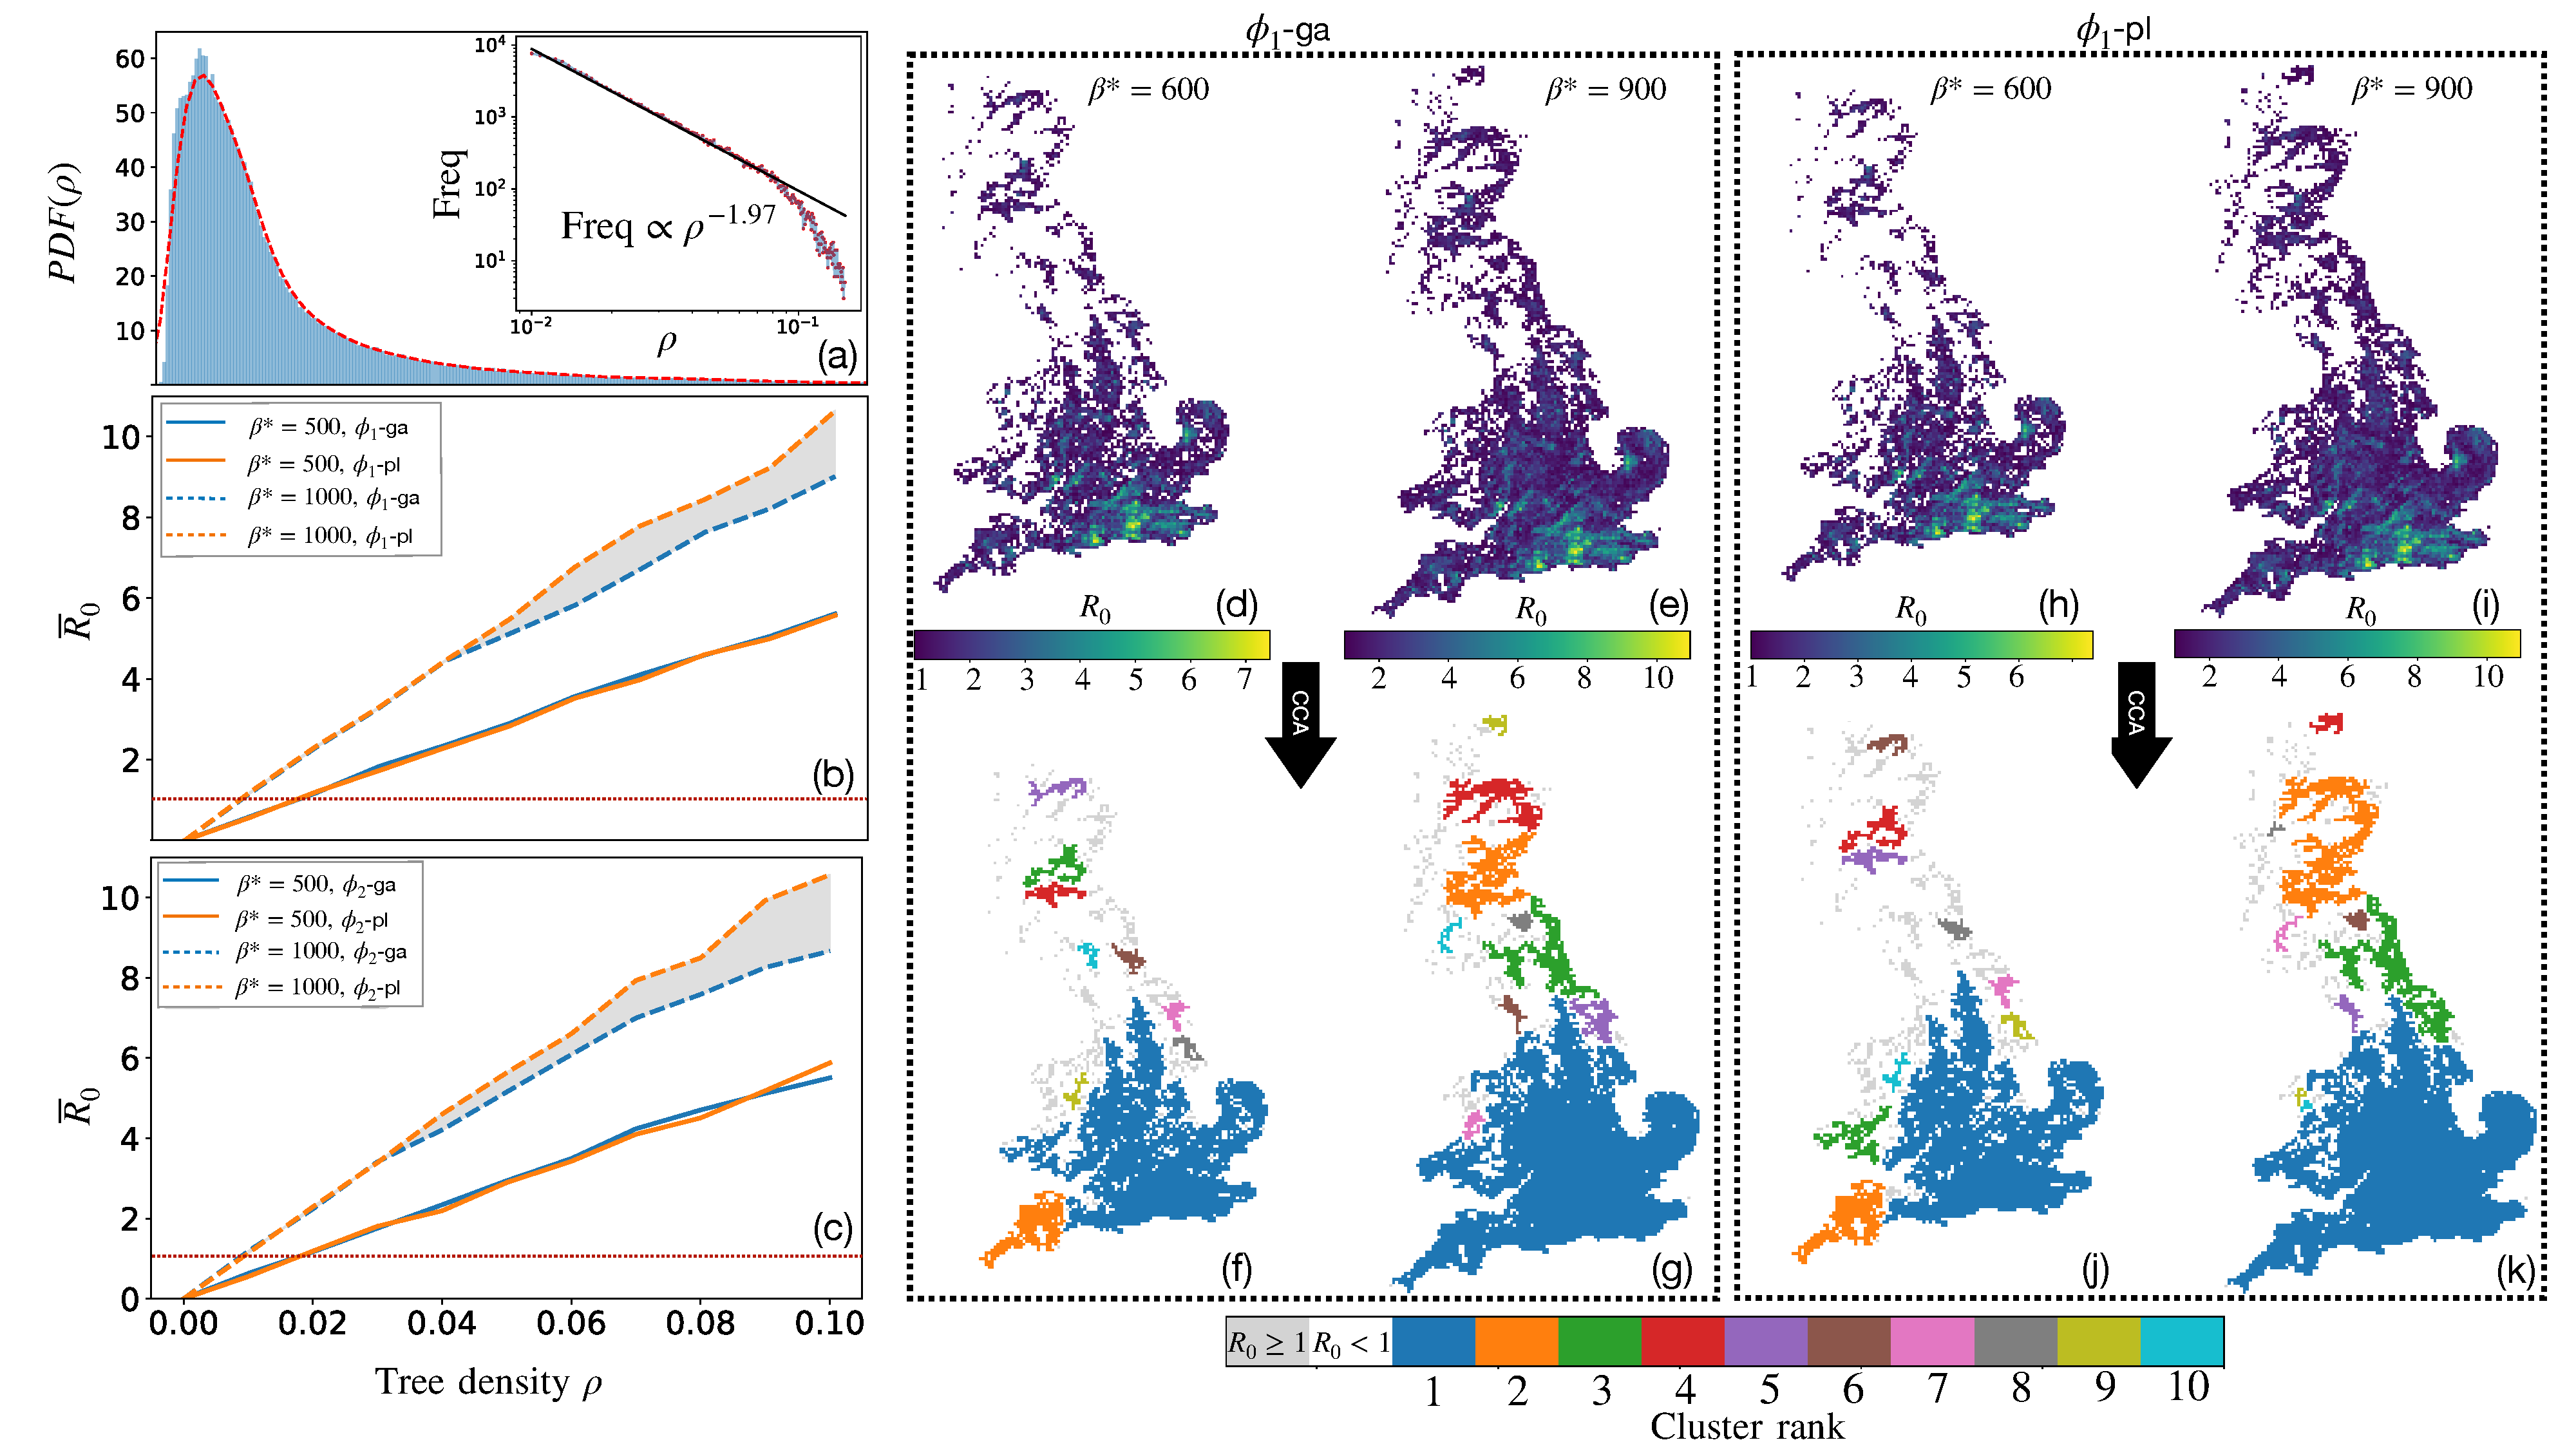
\includegraphics[scale=0.38]{chapter6/figures/fig6-R0-map-generation.pdf}
    \caption{Generating $R_0$ maps for ADB over Great Britain. (a) Ensemble-averaged results of $R_0$ are plotted against the tree densities informed by \cite{hill.data}, revealing a linear relation between $R_0$ and $\rho$. (b-c) Projecting $SEIR$ inverse power law $R_0$ values onto the re-scaled $5\mathrm{km} \times 5 \mathrm{km}$ ash host-distribution for two values of $\beta_{pl}$. Patches of land below $R_0 = 1$ are shown as white space. (d-e) The top $10$ largest connected, and susceptible, $R_0$-clusters that are present in maps (b-c).}
    \label{fig:R0-map-generation}
\end{figure}
\end{landscape}

Figures \ref{fig:R0-map-generation}(d-e) and (h-i) present $R_0$-values of the small-scale $\phi_1$-ga and $\phi_1$-pl $SEIR$ models projected onto the host distribution of ash.
Both sets of $R_0$-maps are projected onto the same coarse-grained $5\mathrm{km} \times 5\mathrm{km}$ re-scaled host distribution.
For all variants of the $SEIR$ model, $R_0$-maps compared similarly\textemdash shown for the two values of infectivity, $\beta^* \in [600, 900]$.
All locations below the transmission threshold $R_0=1$ were given numerical values of zero and are depicted by inland white space.
Under the influence of a more infectious pathogen, larger areas of the ash population become susceptible by supporting the growth and reproduction of the pathogen, illustrated by the difference in patch density in Figures \ref{fig:R0-map-generation}(b-c). 
Importantly, each $R_0$-valued pixel portrays the local-scale epidemic impact experienced at that location, predicted from a five-year ensemble-averaged value of $R_0$.

Suppose that a fitted value of infectivity $\beta^*$ is found to fall within a standard error of $SE=250$,  i.e. $\beta^* = 750 \pm 250$.
In this scenario, epidemic uncertainty is captured by the divergence between dashed and solid lines in Figures \ref{fig:R0-map-generation}(b-c)
and conveniently visualised by differences in the resulting $R_0$-maps.
Although landscape-level heterogeneity and regional susceptibility can be loosely identified from $R_0$-maps in Figures \ref{fig:R0-map-generation}(d-i),
visualising differences between model variants is untenable due to their similarity. 
Furthermore, determining which pixels connect to form susceptible clusters is non-trivial. 
To this aim, the next section will present a means to identify clustering in $R_0$-maps.

\subsection{Clustering in the $R_0$ map}
\label{sec:r0-clustering}

An image processing technique called `connected component analysis' (CCA) was used to identify and label susceptible clusters and simplify the $R_0$-map \cite{CCA1, CCA2} . 
The Python-SciPy package `ndimage' \cite{scipy} was used to implement CCA via the function `label'. 
Doing so labelled all susceptible neighbours as connected members of the same cluster, according to a structuring element \cite{liang1989erosion}. 
That is, if two susceptible patches of ash lie within the same neighbourhood, defined by the structuring element, they are connected members of the same cluster\footnote{Structuring elements have their roots in shape, and image analysis \cite{23111}, where they define how distinct binary shapes connect to form images \cite{liang1989erosion, nachtegael2001connections}}. 
Additional information on structuring elements and CCA can be found in Appendix \ref{a:CCA}.

Moore and Von-Neumann neighbourhoods were chosen as structuring elements to classify connected components\textemdash a comparative look exploring the differences between Von-Neumann and Moore 
structuring elements is resumed below in sections \ref{sec:inverse-power-law-r0-clustering}-\ref{sec:gaussian-r0-clustering}.  
Figures \ref{fig:R0-map-generation}(f-k) correspond to the top ten largest connected $R_0$-clusters (by area $\mathrm{km^2}$) present in the $R_0$-maps of Figures \ref{fig:R0-map-generation}(d-i) according to the Moore neighbourhood.
For both dispersal models, increasing the infectivity parameter $\beta$ leads to a more susceptible and connected $R_0$-map, as demonstrated by the larger dominating cluster in Figures \ref{fig:R0-map-generation}(g) and (k).

There are little to no differences between how Gaussian and inverse power law models spatially scale, according to the raw $R_0$-maps of Figures \ref{fig:R0-map-generation}(d-i).
However, CCA reveals some subtle differences in the projection of $\phi_1$-ga and $\phi_1$-pl under the same normalised infectivity parameter $\beta^*$.
Although, given similar gradients in the graph of $R_0$ versus $\rho$ for lower infectivity values
\textemdash demonstrated by the convergence of solid orange and blue lines in Figures \ref{fig:R0-map-generation}(b-c)\textemdash 
Gaussian and inverse power law models should produce the exact $R_0$-map.
In contrast, for higher infectivity parameters, we might expect the inverse power law model to yield a more susceptible map, as per Figures \ref{fig:R0-map-generation}(b-c) when the Gaussian model deviate below linearity.

For the infectivity parameter $\beta^*=600$, model $\phi_1$-ga shows that the largest `dominating' cluster (in blue) extends over a slightly larger area than for model $\phi_2$-pl.
In Figure \ref{fig:R0-map-generation}(j), the third-largest cluster (in green, located in Wales) remains disconnected from the largest dominating cluster (shown in blue),
whereas in Figure \ref{fig:R0-map-generation}(f) the corresponding clusters are connected. 
In a similar vein, Figure \ref{fig:R0-map-generation}(k) shows a larger dominating cluster than Figure \ref{fig:R0-map-generation}(g).
However, differences are seen most visibly over Scotland and Northern England (Humber-Northumbria), where the second and third largest-ranked clusters extend over more significant areas.
Nevertheless, differences in how dispersal models scale over GB are primarily trivial, and stochasticity in ensemble-averaged $R_0$-values could likely explain any differences.

\subsection{Interpreting susceptible $R_0$-clusters}

Given that disease gradients can extend over $10-1000\mathrm{km}$, we cannot preclude the possibility of secondary infections spreading between clusters.
Alongside jumping directly over below-threshold patches, the pathogen may use intermediary trees inside below-threshold patches as stepping stones and jump between clusters indirectly. 
Conceptually, this has been described for pathogens jumping between crop fields \cite{Gilligan-disease-management} and more abstract modelling work \cite{wingen2013long}.
In a simplified interpretation, the model presents two distinct types of spread, within-cluster and between-cluster spread. 

Here, within-cluster connectivity is sufficient for uninhibited spore-dispersal between nearest-neighbour patches in the $SEIR$ model of ADB.
Moreover, the disease may spread over large spatial scales even without the need for LDD\textemdash without directly or indirectly, jump between nearest-neighbours.
Thus, high-risk areas can be simplistically identified in the $R_0$-map.
Next, a closer look at $R_0$-clustering is conducted.

\subsection{Inverse power law $R_0$-map clustering}
\label{sec:inverse-power-law-r0-clustering}
% explain basic behaviour, 5km spatial structure

In the small-scale $SEIR$-model of ADB, inverse power law dispersal required a domain size of $\mathrm{5km \times 5km}$ to accurately gauge $R_0$ over the mean infectious lifetime of ADB.
Domain size, $L$, in the inverse power law $SEIR$ models, therefore, motivate a coarse-grained host distribution.
Consequently, when spatially scaling the inverse power law model over Great Britain, each pixel reflects a $\mathrm{5km \times 5km}$ patch of land at minimum.
It would be possible to possible to coarse-grain to lower resolutions, e.g. $\mathrm{10km \times 10km}$.
Although as Figure \ref{fig:ash-host-data}(b) eludes to, landscape-level spatial structure is lost in the process.
Therefore, the inverse power law models $\phi_1$-pl and $\phi_2$-pl were explored over a single landscape-level resolution of $\mathrm{5km \times 5km}$.

For each value of infectivity, an $R_0$-map will contain a variety of differently sized $R_0$-clusters.
Figure \ref{fig:inverse-power-law-clustering} presents $R_0$-clustering behaviour for the inverse power law model.
A proper understanding of clustering can be achieved by exploring how the distribution of cluster sizes change in response to infectivity. 
Figures \ref{fig:inverse-power-law-clustering}(a) and (c) show the frequency distribution of cluster sizes, 
for models $\phi_1$-pl and $\phi_2$-pl respectively.
The distributions depict cluster sizes for three infectivity parameters $\beta^* \in [250, 500, 1000]$ according to the Moore neighbourhood.
In both frequency distributions, a small proportion of large dominating clusters can be seen alongside more numerous smaller $R_0$-clusters.

Unsurprisingly, a lower infectivity parameter reduces the size of the highest-ranked cluster and lowers the overall coverage of susceptible $R_0$-clusters\textemdash shown in blue.
Increasing the infectivity produces a larger dominating cluster but reduces the mean size of lower-ranked $R_0$-clusters, 
understood by contrasting the orange and green frequency distributions.
The inset plots of Figure \ref{fig:inverse-power-law-clustering}(a) and (c) depict the same behaviour in a rank-ordered list of the top 25 largest $R_0$-clusters by size.
Both sporulation models display the same fundamental relationship.

\begin{figure}
    \centering
    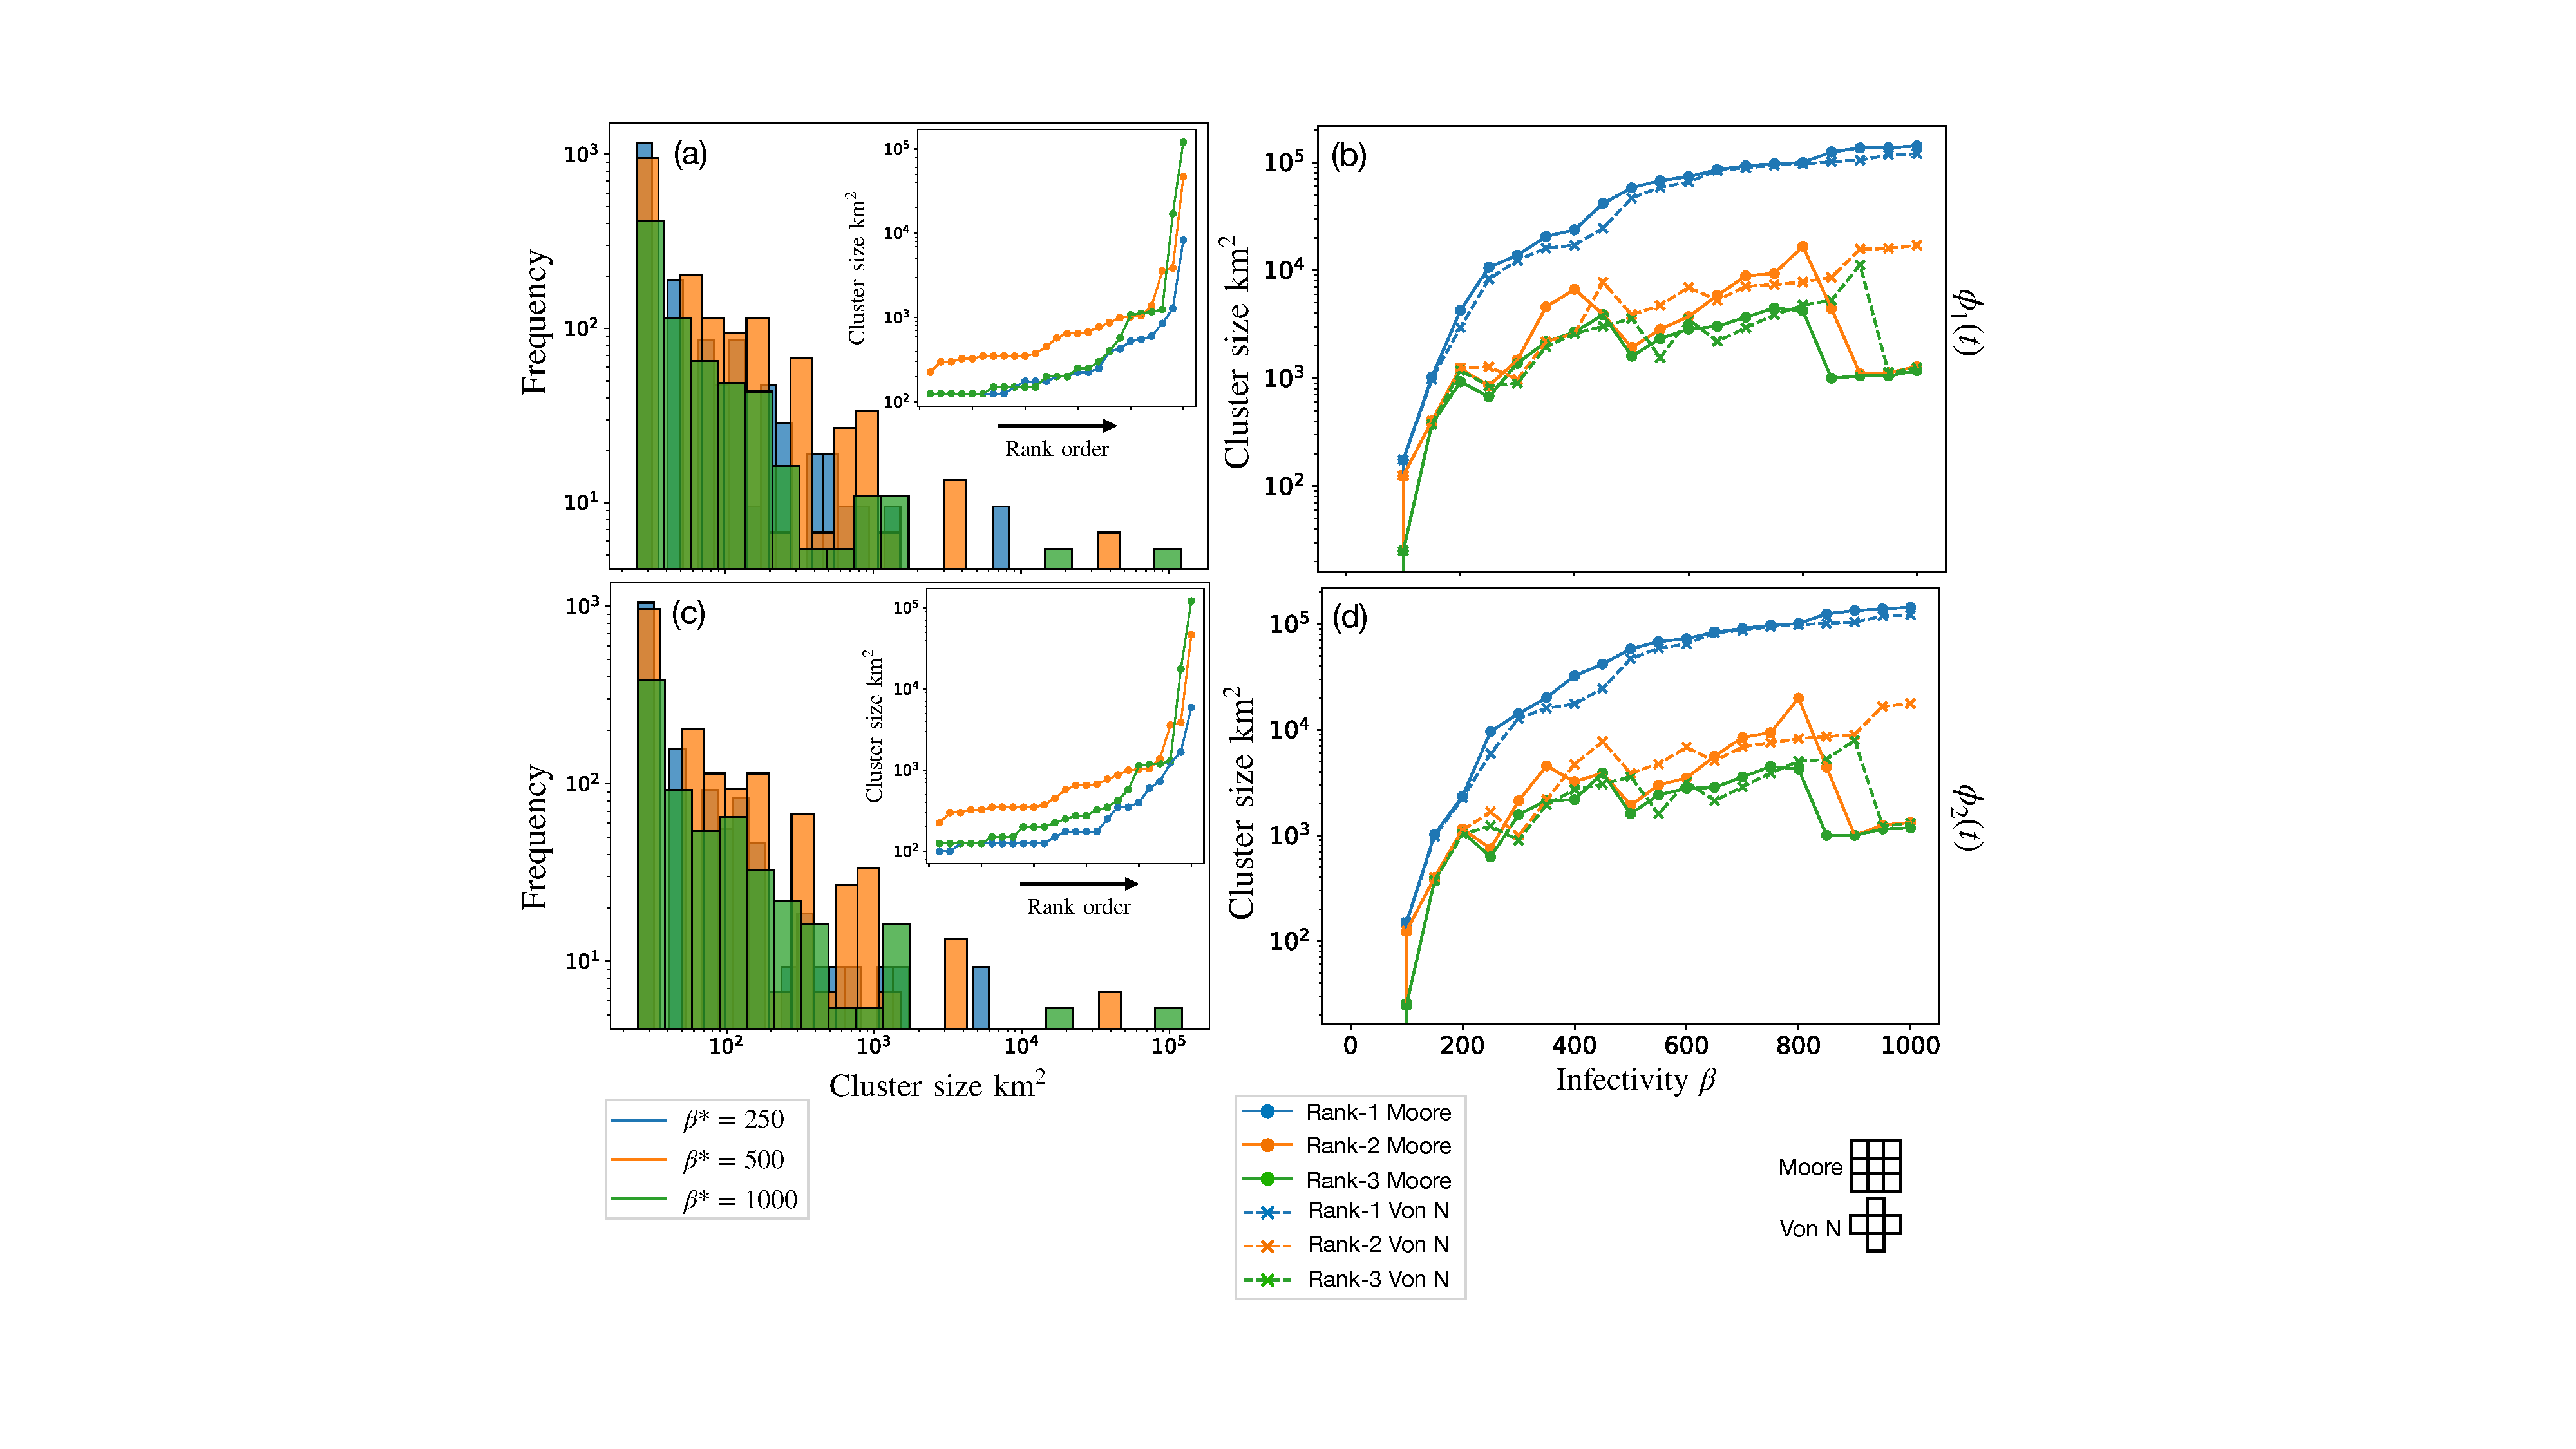
\includegraphics[scale=0.45]{chapter6/figures/fig6-pl-cluster-distribution.pdf}
    \caption{Susceptible $R_0$-clustering for the inverse power law model (a) For model $\phi_1$-pl, the cluster-size frequency distribution is shown for three infectivity values utilising the Moore neighbourhood. The inset shows a rank-ordered graph of the top $25$ most significant clusters by area $\mathrm{km^2}$. (b) The top three ranked clusters, by size, for model $\phi_1$-pl is shown over the infectivity parameter-space for both Moore and Von-Neumann neighbourhoods. (c) The frequency distribution of cluster size is shown for the peaked sporulation model $\phi_2$-pl for three infectivity parameters (d) Cluster-size behaviour for model $\phi_2$-pl shown over infectivity parameter-space for Moore and Von-Neumann neighbourhoods.}
    \label{fig:inverse-power-law-clustering}
\end{figure}

In the $SEIR$ model, a value of $\beta$ has not been determined experimentally or statistical fitted.
Therefore, we are compelled to study behaviour over the entire space of $\beta$.
Figures \ref{fig:inverse-power-law-clustering}(b) and (d) describe how $R_0$-clusters scale over different values of infectivity and structuring elements for models $\phi_1$-pl and $\phi_2$-pl respectively.
As infectivity is increased to a maximum of $\beta^*=1000$, the largest $R_0$-cluster (shown in blue) rises most rapidly over a narrow range of infectivity values in the interval $\beta^*\in [100, 400]$.
Patches are more likely to become susceptible as $\beta^*$ increases; this causes rank-1 $R_0$-clusters to amalgamate surrounding neighbouring clusters as channels open up.
Thus, fluctuations arise in the second and third largest clusters as they form an ever-larger dominating cluster.
Below $\beta^*=100$, no cluster-growth is displayed as epidemic parameters are too low. 
 
Up to this point, we have considered one structuring element, namely the Moore neighbourhood.
The type of structuring element we choose to gauge regional-susceptibility in the $R_0$-map bears no influence on how an epidemic might progress in reality.
Therefore, it is desirable for clustering in the model to remain invariant over the structuring element we choose.
In general, visible, albeit small, differences can be seen due to artefacts of the structuring elements.

Moore neighbourhoods can be seen to produce slightly larger rank-1 $R_0$-clusters, which in turn reduced the size of second and third-ranked clusters.
The disparity caused between structuring elements can be understood by noting the two additional corner/diagonal pieces in the Moore neighbourhood.
Although structuring elements account for a comparatively small deviation between cluster sizes, the rank-1 clusters compared similarly for some values for $\beta^*$.
Observing minor artefacts due to structuring elements hint toward limitations in the definition of connectivity, as defined within the landscape-level component of the model.

\subsection{Gaussian $R_0$-map clustering: varying map resolution}
\label{sec:gaussian-r0-clustering}

The essential dynamic of $R_0$ clustering holds when spatially scaling the Gaussian-based models $\phi_1$-ga and $\phi_2$-ga.
Notwithstanding some negligible cluster size differences, as demonstrated above in Figure \ref{fig:R0-map-generation}.
However, as explored in section \ref{sec:r0-vs-L}, $R_0$-values in the more localised Gaussian dispersal models can be discerned inside a domain size of $\mathrm{1km \times 1km}$.
Given that $R_0$ can be captured inside a smaller domain, we may consider resolving $R_0$-maps to a finer landscape-level resolution in comparison to the inverse power law-based dispersal models.
Resolving $R_0$-maps to the highest resolution possible is desirable to apprehend the nature of epidemic severity and spatial heterogeneity.
Otherwise, relevant epidemic information is lost when coarse-graining the host distribution. 

Figure \ref{fig:gaussian-clustering-A} shows how CCA changes clustering in the $R_0$-map for different landscape-level resolutions.
Figures \ref{fig:gaussian-clustering-A}(a-c) show the frequency distributions of cluster size for $\beta^*=500$ and three different patch sizes, of lengths $\mathrm{5km,\ 3km,\ 1km}$ respectively.
As discussed in section \ref{sec:inverse-power-law-r0-clustering}, the same general trend remains, i.e. a small number of large clusters alongside more numerous small clusters.
Although, decreasing the patch size produces a more fragmented domain, indicated by the greater variety of cluster sizes.
The largest ranked cluster toward the far-right of each distribution also shrinks for successively smaller patch sizes.
However, decreasing the patch size brings frequency distributions between structuring elements into closer alignment, seen by a closer agreement of blue and orange distributions in Figure \ref{fig:gaussian-clustering-A}(c).

As before, cluster size for the largest ranked cluster exhibits the most significant growth over the first few values of infectivity, 
$\beta^* \in [100, 400]$. However, performing CCA at different landscape-level resolutions produces a change in the size of $R_0$-clusters.
At the most extreme point of $\beta^*=500$, more significant deviations can be seen between the size of rank-1 susceptible $R_0$-clusters,
illustrated by the vertical arrow in Figure \ref{fig:gaussian-clustering-A}(d).

Figures \ref{fig:gaussian-clustering-B}(a-c) depict visual differences of CCA at domain resolutions: $\mathrm{5km \times 5km}$, 
$\mathrm{3km\times 3km}$, and $\mathrm{1km\times 1km}$.
We witness similar landscape-level features for each domain resolution in the largest ranked $R_0$-cluster (in blue), 
though disparities exist in the extent and size of clusters. As the $R_0$-map is resolved to a small spatial-scales, 
connectivity within an $R_0$-cluster can depend more critically on a small number of above-threshold patches, 
identified by the red circles in the inset in Figure \ref{fig:gaussian-clustering-B}(c).

In the coarse-grained $\mathrm{5km\times 5km}$ resolution domain of Figure \ref{fig:gaussian-clustering-B}(a), 
the critically-connecting patches circled in Figure \ref{fig:gaussian-clustering-B}(c) are smoothed in the process of averaging the small number of surroundings patches. 
Similarly, some above-threshold patches can be smoothed to below-threshold patches, thus increasing the cluster size, shown in Figure \ref{fig:gaussian-clustering-B}(b) circled in red.
Ultimately, differences in cluster size are caused by the simplistic notion of connectivity within CCA that fails to scale with the domain resolution.
Undesirably, witnessing a difference in CCA-identified clusters outlines an inherent limitation of the framework.
Even though clusters appear different, these observations emphasise that connectivity over a region can depend on a small number of patches, 
which sets the scene for Chapter \ref{ch7:landscape-level-control}.

\begin{figure}
    \centering
    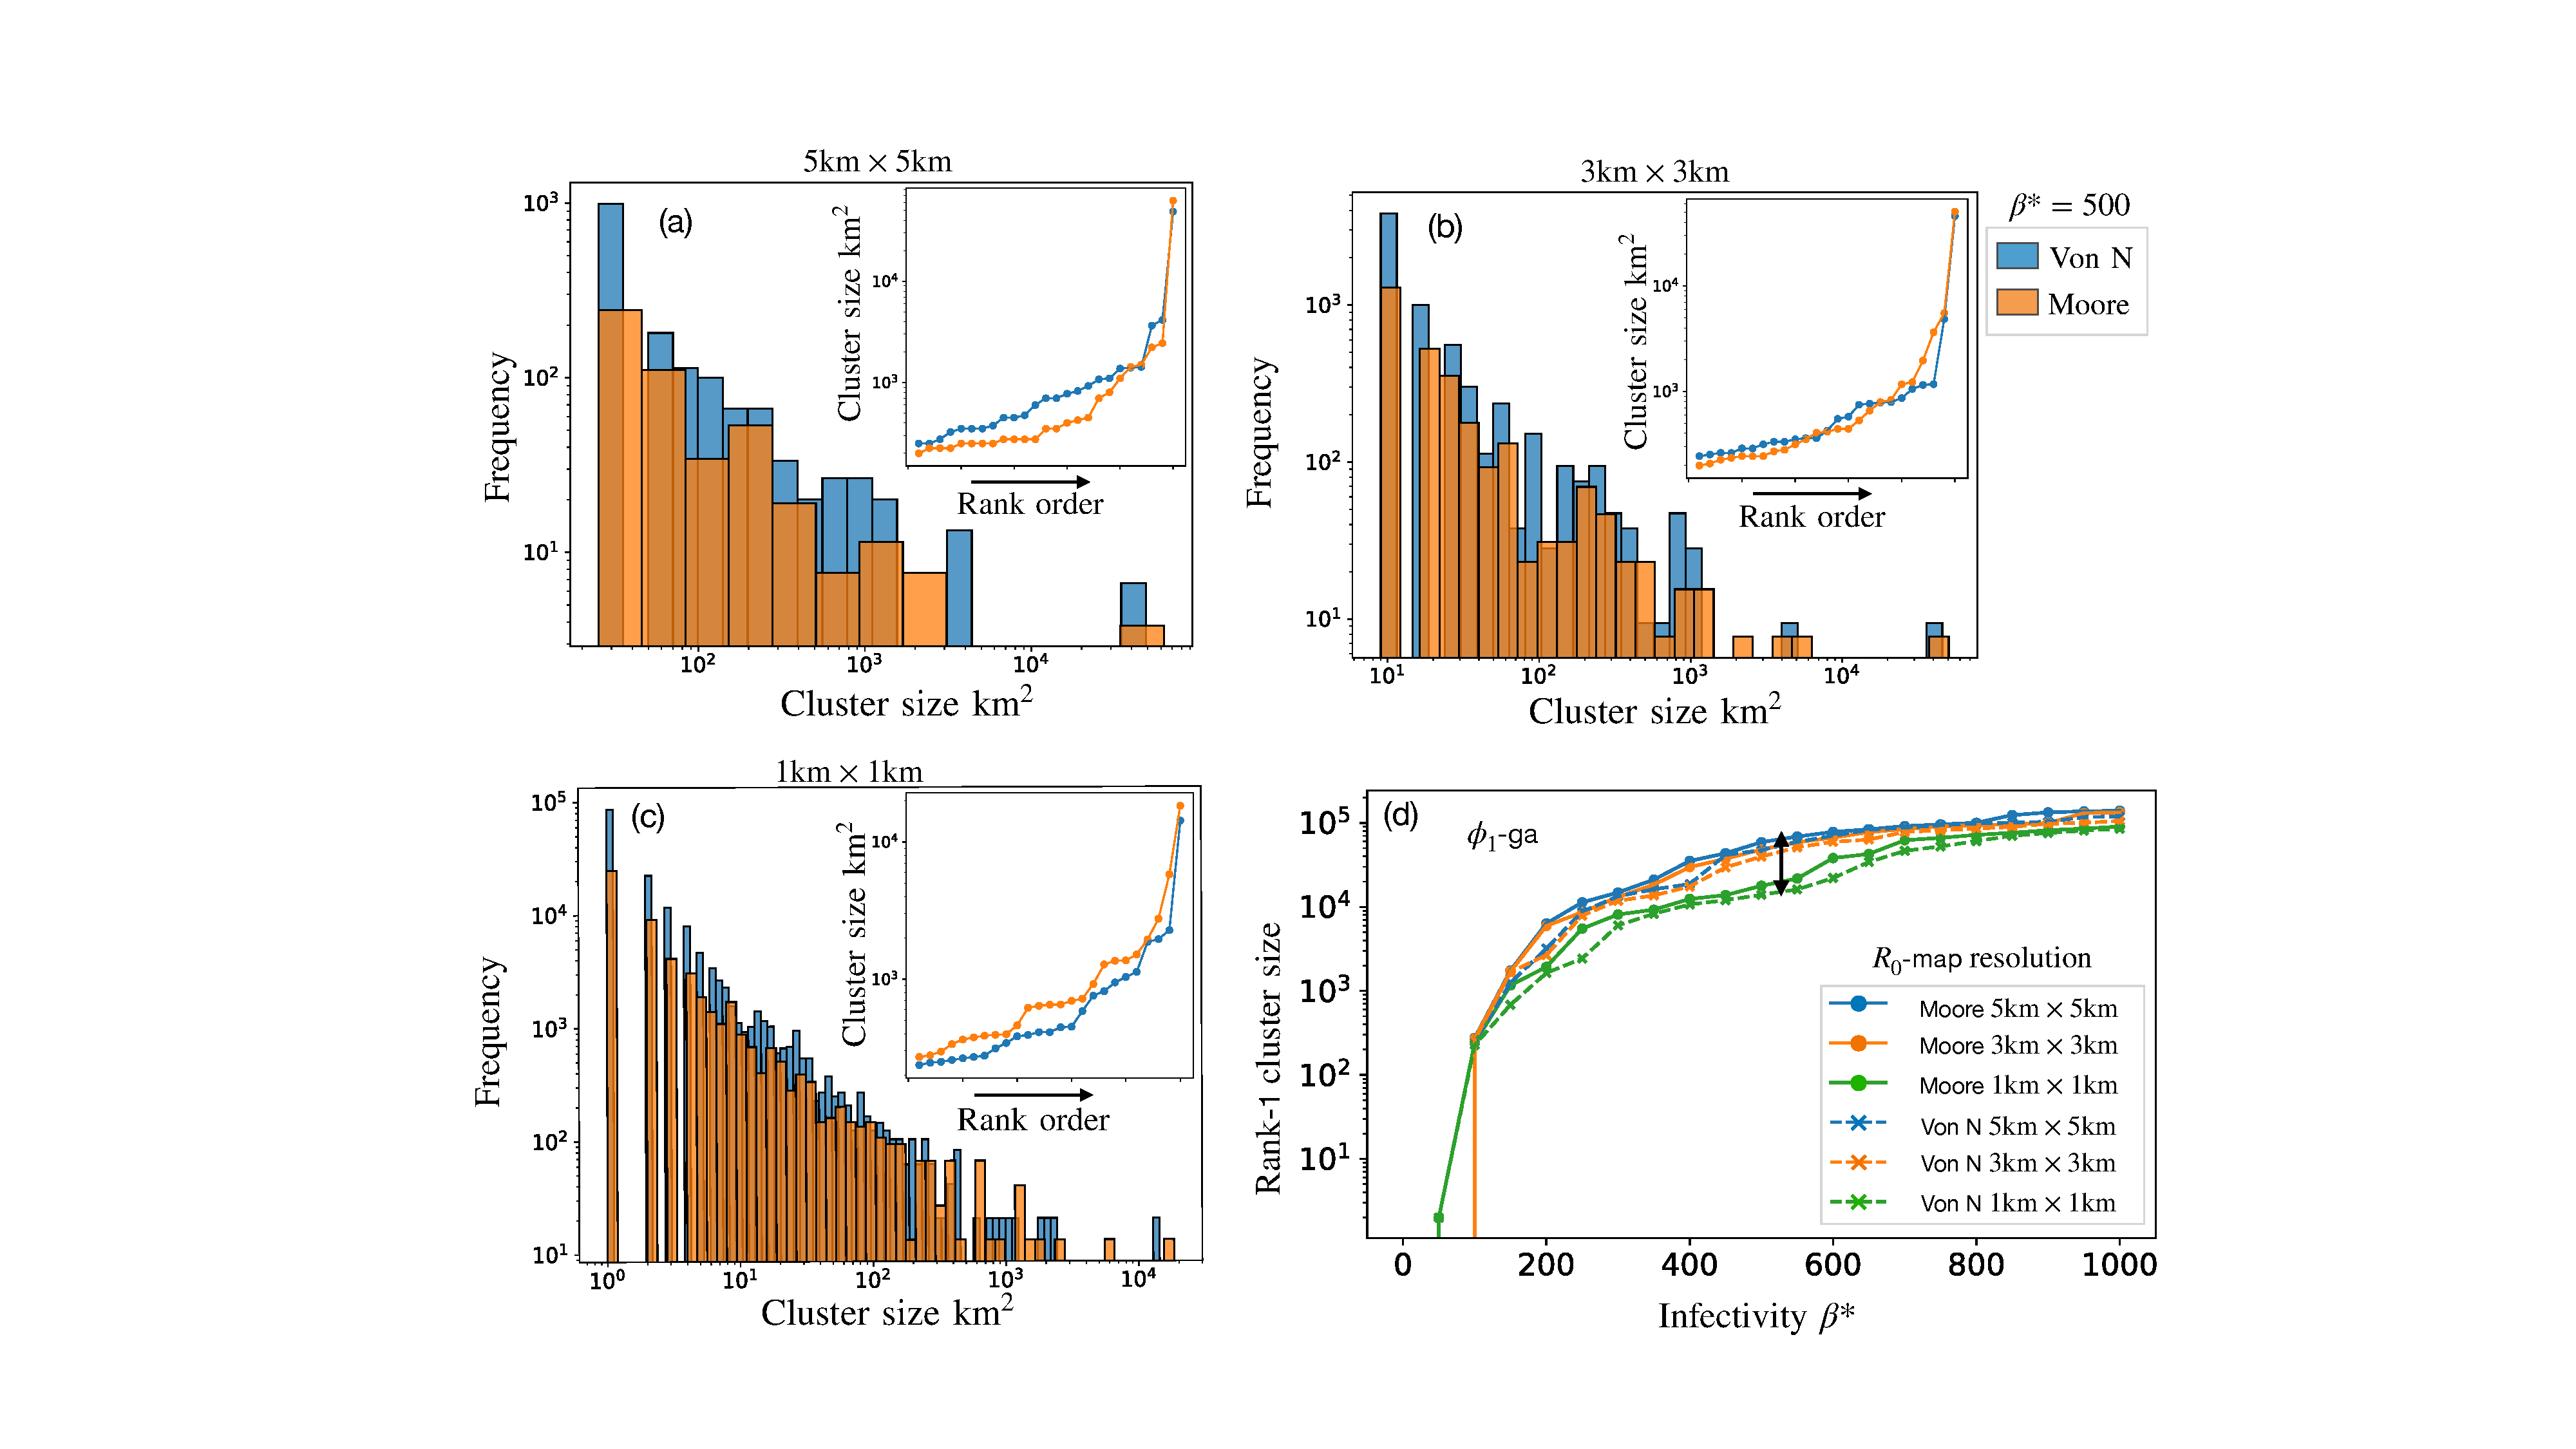
\includegraphics[scale=0.375]{chapter6/figures/fig6A-ga-cluster-distribution.pdf}
    \caption{
    Multi-scale CCA performed over different landscape-level resolutions, namely from $\mathrm{1km \times 1km}$ to $\mathrm{5km \times 5km}$ patch-sizes. 
    (a-c) Cluster-size distributions are shown for three landscape-level domain resolutions and both Moore and Von-Neumann structuring elements. 
    As domain resolution is increased to $\mathrm{1km \times 1km}$, clusters can be resolved to a finer scale and yield a set of clusters over more length-scales 
    (d) Cluster sizes over infectivity $\beta^*$ and structuring elements, comparing behaviour at two pixel-sizes. 
    At the most extreme point, large disparities in cluster sizes become apparent, indicated by the vertical arrow at $\beta^*=500$.}
    \label{fig:gaussian-clustering-A}
\end{figure}

\begin{figure}
    \centering
    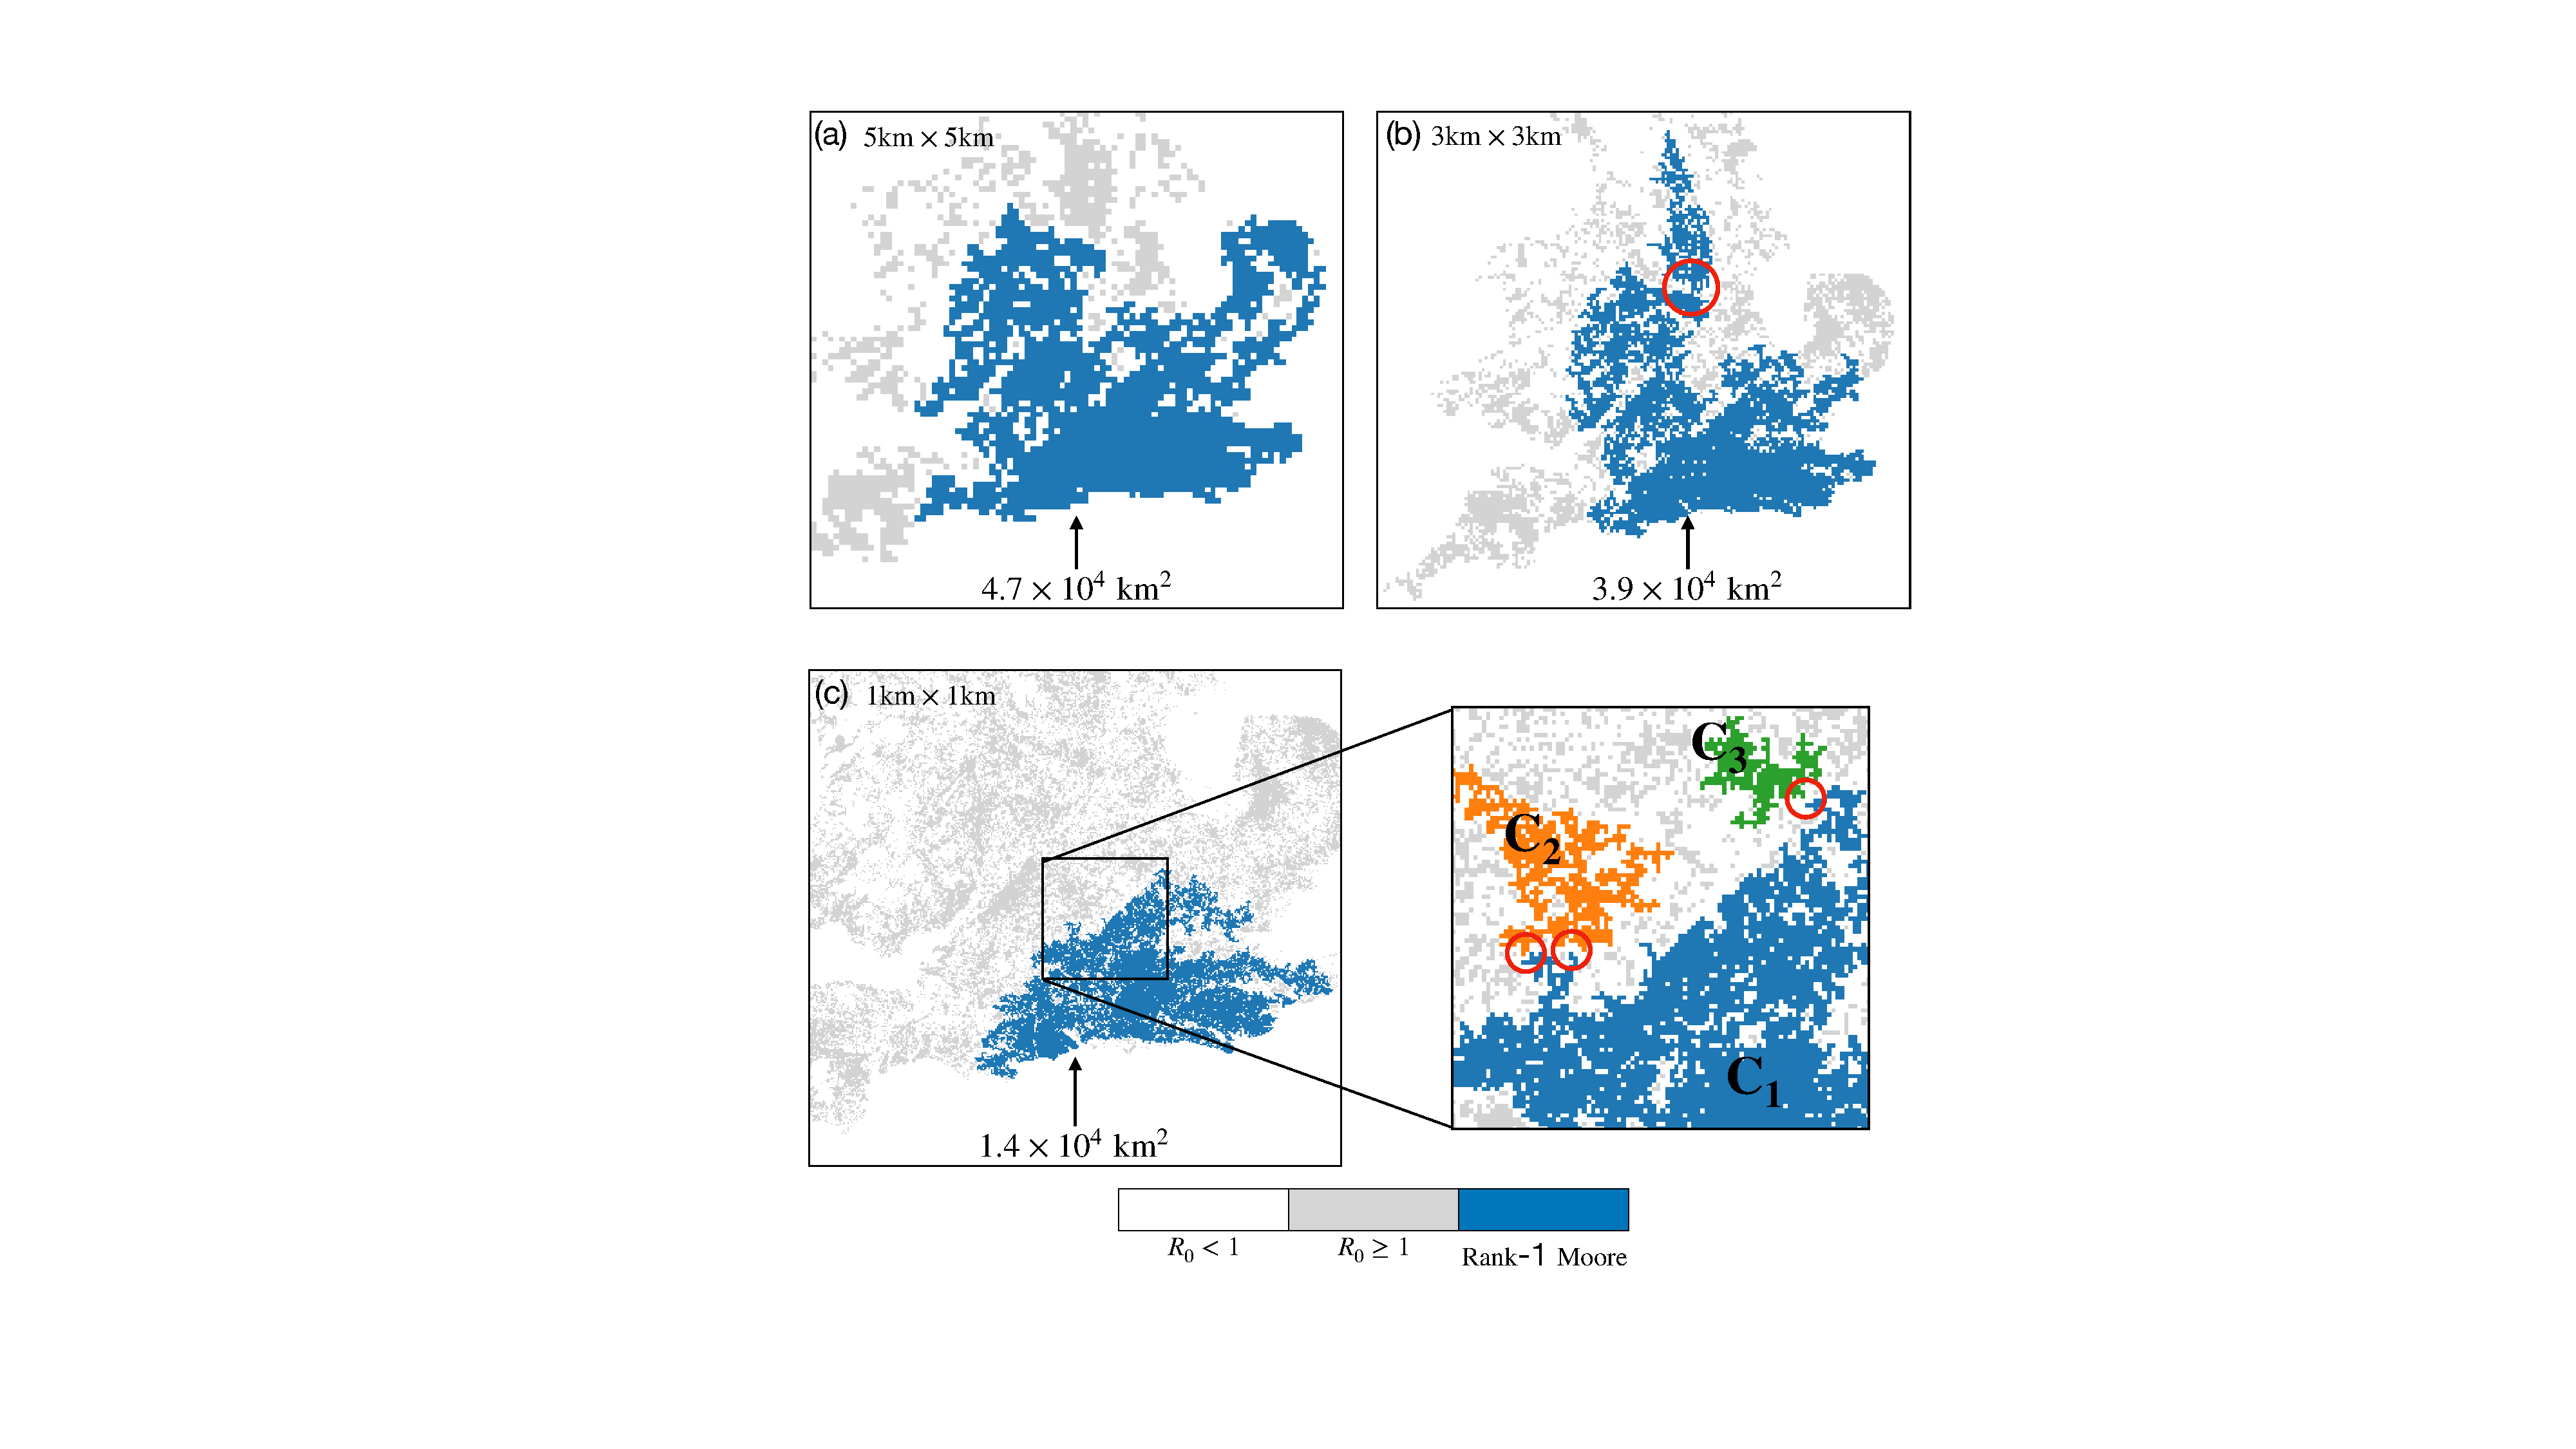
\includegraphics[scale=0.55]{chapter6/figures/fig6B-ga-cluster-distribution.pdf}
    \caption{ 
     Spatial interpretations of Figures \ref{fig:gaussian-clustering-A}(a-c), according to the Moore neighbourhood, are shown for $\beta^*=500$
     and different patch resolutions. 
     For each domain resolution considered, the largest ranked cluster appears different, pointing to an inherent limitation in the framework
    (a) The largest ranked $R_0$-cluster is shown in blue for the most coarse domain at resolution $\mathrm{5km \times 5km}$ 
    (b) Resolving $R_0$-valued patches to a $\mathrm{3km \times 3km}$ resolution can lead to extra patches opening up 
    (i.e. becoming susceptible $R_0 > 1$) to form connections between other, distinct $R_0$-clusters. 
    Here, patches circled in red form a bridge to a previously disconnected cluster 
    (c) Resolving $R_0$-valued patches to the highest resolution of $\mathrm{1km \times 1km}$ causes a more fragmented domain. 
    A small number of below-threshold patches can fragment the $R_0$-cluster, highlighted in red.
    }
    \label{fig:gaussian-clustering-B}
\end{figure}

\section{Discussion and future work}

The work presented in this Chapter describes how to project a spatially explicit, small-scale compartmentalised model onto a host distribution.
The method to `spatially scale' a small-scale epidemic model is computationally inexpensive, flexible and generalisable.
Here, results are focused on helping policymakers implement informed decisions about \textit{where} to control the spread of disease, based on spatial arguments.
In the face of low budgets, limited resources and short decision windows, an efficient method to prioritise targeted control could aid both policymakers and (tree health) stakeholders.

Given the sessile nature of trees, the spatial distribution of hosts remains of paramount importance for epidemic modelling.
As such, a modelled distribution of ash covering Great Britain was used to parameterise host densities.
This choice was motivated by the non-existence of freely available, high-quality ash abundance data that spans Great Britain.
Consequently, combining our small-scale $SEIR$ model with data given by \cite{hill.data} demonstrates a novel use of predicted abundance data\textemdash
as remarked when summarising the toy SLM model of Chapter \ref{chapter:SLM-applications}.

Due to the complexity of ADB, some important assumptions had to be employed in the $SEIR$ model.
In particular, leaf-shed was assumed to fall close to ash hosts; 
this permitted fungal ascospore dispersal to originate from the same location as infected ash.
Still, this assumption is supported by the dispersal parameterisation given by \cite{grosdidier2018tracking} that measured dispersal directly between a source of infected trees and spore-traps, thereby omitting the dynamics of intermediary leaf-shed dispersal.
One possible improvement to the $SEIR$ model might include host demography, as host-pathogen coexistence is not supported.

Performing CCA proved a beneficial yet problematic exercise.
Multi-scale CCA demonstrated how failing to include relevant epidemiological information, in the form of coarse-grained host data, can lead to significant disparities in cluster size\textemdash sentiments echoed in the third challenge posed by \cite{13-challenges}.
Furthermore, resolving Gaussian $R_0$-maps at different landscape resolutions emphasises an implicit assumption when defining connectivity based solely on nearest-neighbour interactions between patches. 
That is, Moore and Von Neumann structuring elements do not scale with the dispersal kernel under a change of map resolution:

\textit{Suppose secondary infections can be induced up to a maximum distance of $D_{max} = 2\mathrm{km}$.
Resolving the map to $\mathrm{2km \times 2km}$ (or lower) is permissible because patches interact locally i.e. infections between non-nearest neighbour patches are unlikely (neglecting atmospheric of human-mediated LDD).
In contrast, suppose the map is now resolved to $\mathrm{1km \times 1km}$.
In this scenario, patches have the possibility of interacting non-locally because $D_{max}$ exceeds intermediary patches;
nearest-neighbour structuring elements therefore fail to describe connectivity accurately.}
Given all the above, an improved understanding of the connectivity between patches is required to progress the framework.

In a nutshell, multi-scale CCA questions the very notion of constructing $R_0$-maps for systems described by fat-tailed dispersal kernels.
The invasiveness of a pathogen described by a fat-tailed dispersal kernel cannot be defined by $R_0$ reliably inside a small domain.
Therefore, epidemic maps depicting inverse power law $R_0$-values require a larger patch size that motivates a coarse-grained host distribution, lowering map resolution.
Omitting finer-scale epidemic information can lead to disparate results, witnessed by varying the Gaussian-based $R_0$-map patch-size.
Thus, mapping $R_0$ values for inverse power law dispersal is called into question.

Despite the limitations of CCA, clusters grew up to four orders of magnitude over the initial interval of infectivity, $\beta^*\in [100, 400]$.
Rapid cluster growth between $\beta^*\in [100, 400]$ occurred for all $SEIR$ model-variants and domain resolutions considered.
Landscape-level spread within our framework, therefore, demonstrates a threshold-like behaviour, below witch ($\beta^* \lessapprox 100$), no models would be able to invade Great Britain.
The next valuable step would be to fit a value of $\beta$ to data on ADB spread\footnote{Given the high availability of ADB mortality data in different European countries, fitting the $SEIR$ model to mortality curves would be most accessible.}, 
and construct the resulting $R_0$-map.

% \section{Chapter summary}

% Where we consider spatial structure and others have not
% - In this chapter, we focused on disrupting local-level dispersal by implementing control at landscape-level.
% -  In this chapter we undertook the ambitious task of scaling up a small-scale model, to large spatial distances covering GB, and developed a new approach to controlling the spread of disease.
% - introduce the regime of pathogen spread we are interested in, we are not modelling continental long-range spread via upper atmosphere, nor are we interested in long-range human trade networks. We are interested in dispersal at the local level whereby passive means of wind, soil and or insects/animals. 

% link to 13 challenges: -- it is your friend...
% 1 - host data is hard to integrate into models \cite(13 challenges), we demonstrate how how this can be achieved
% 2. primed a model of multi scale, although we have not included LDD spore transport, the framework serves to include this via a more complete treatment of the structuring element
% 3. capturing time-varying infectivity is hard \cite{13 challenges},
% 4. constructing a spatial model of disease severity could help to deploy resources to known locations e.g. monitoring
%5. web api to help policy makers

% The work conducted in this chapter are focused toward help policy makers implement informed decisions, about \textit{where} to control the spread of disease, based on spatial arguments.
% The framework we implemented was constructed using a simplified model of ADB, although the method is flexible and can be generalised for other compartmentalised models, provided sufficient host data and fitted epidemiological parameters. 
% In the face of low Identifying which locations are likely to support the highest epidemic severity is key for targeted control when budgets are low\textemdash as noted by \cite{time-varying-infectivity}. Our approach of spatially scaling small-scale epidemiological principles was conducted through computational, opposed to analytical, means. 

% % The scaling up of our model
% The scaling up of our model resembles a metapopulation model, now commonplace when modelling plant-based epidemics, but crucially our large-scale model is not dynamic. A dynamic large-scale model is indeed useful for the prediction of time-scales and the movement of disease-fronts movement; however, we suggest they might be at best less useful for optimised large-scale control, and at worse, nicely complemented by the approach we develop.

% If early data through a particular region, with known data, was collected, it would be a relatively short step to fit the dispersal model and scale up the model over large distances given the seemingly simple relation to host density $\rho$.
% % At the small scale we have a uniform population. However for larger scales we have considerable spatial heterogeneity.
% % spatial-scale and control, over a multi-seasonal pathosystem, have been investigated for sugar beet in the UK, see \cite{doi:10.1146/annurev.phyto.45.062806.094357} for a review.


% % On the SEIR model

% The cyclic nature of the $SEIR$-type model constructed in this article can also find resemblance in the, well established body of literature, of crop-based epidemics. It is common-place for a field of crops to become infested, then at the end of the growing season be totally eradicated by virtue of harvesting 
% % there is a surprising lack of, simplified, ash dieback models in the literature...\ciations... <-- double, triple and quadruple check!
% % without host demography 
% % landscape level control strategy
% % Therefore, not modelling the asexual component of ADB represents an important assumption in the model.
% % , both spatial and genetic variations are known to influence the epidemic progression of ADB \cite{stocks2017first, mckinney2014ash}. 
% % Observations of ADB invasions suggest a strong on the surrounding landscape features \cite{https://doi.org/10.1111/1365-2745.13383}.
% % Here, the function $\phi_2(t)$ is a special case of the Gamma(k) presented in \cite{time-varying-infectivity}.

% % Adopting a compartmentalised $SEIR$-like structure to model the spread of ADB at local spatial-scales is both novel and ambitious
% % \footnote{Models of plant-based fungal pathogens with comparable life-cycles have typically opted for different approaches e.g. the ascomycete `apple scab' \cite{rossi2007scab}}.

% % Fitting the seasonal $SEIR$ model of ADB to ash mortality data would therefore be most tenable. In practice, fitting could be explored by varying $\beta$ until the mortality curve resembles experimental data

% % multi-scale approaches have been outlined \cite{hart2020theoretical}
% % multi-seasonal frameworks comprise a common theme in the spread of crop-based epidemics see  x, y, and typically involve soil-borne nematodes-based outbreaks \cite{tankam2020modelling} <- see references inside.

% % \cite{time-varying-infectivity} has 
% % we contend the SnIEmR model, considered over one sporulation peak, is a simplistic implementation of the SEIR-based model needed to compute an invasion threshold that represent the infection dynamics ash dieback. 
% % The SEIR-based model is made more flexible, and can be readily extended or adapted to incorporate more biological realism, by virtue of splitting the E and I into multiple compartments\textemdash this is frequently done in human and animal-based models \citations..

% % - time varying infectivity parameter for ADB \beta could be subject to increase in response to the warmer conditions presented by climate change \cite{magarey2005simple}
% % - Interestingly, ash dieback could be adversely effected be climate change \cite{goberville2016climate}


% %- Although the main result of our work was conduced over one sporulation peak, or life-cycle of ash dieback, splitting the model into various compartments was a useful and necessary step towards developing accurate large-tree species. reference  \cite{https://doi.org/10.1111/ppa.12894} alludes to multiple exposed periods being useful

% %- A quantity of interest that appears frequently in the literature is the initial growth rate $r$, that is the density-independent growth at the start of any epidemic.
% % See \cite{ferrandino2012time} for a review on the time-scales and sporulation of plant-based diseases.

% % Fitting data to the early phases of an epidemic has been shown to give large differences in the final-size epidemic, or severity \cite{time-varying-infectivity}. However, we are only interested in a pathogens ability to invade and this can be closely approximated by measuring R0 over the fist observation (\see appendix)
% % fitting....- Although, various data regarding ash mortality after years of infection have been published in various countries, as reviewed in chapter \ref{ch2:ash-dieback}.
% % The variability between the particular life-cycle history followed by hosts is thought to be an important factor to consider\cite{ferrandino2012time}, and we intentionally neglected this for the purpose of simplicity...

% % subdividing compartments in this manner could also provide an easier implementation to hosts which become more infectious, through a greater production of spores, as the infectious cycle continues not to mention particular periods of environmental unsuitability.
% %

% % Accurately modelling time-varying infectivity is difficult \cite{13-challenges}, and as such, we opted for parsimony.

% % Main assumptions in the method: 
% % 1) Assumptions about dispersal
% Dispersal over small spatial-scale is thought to predominately occur passively through wind, however other means of dispersal exist such as soil and or insects. There are many pathways a pathogen can use to spread through a landscape, including long-range dispersal, mediated through either human-trade networks %
% \cite{hulme2009trade, banks2015role, chapman2017global} or dispersal in the upper atmosphere \cite{westbrook1999atmospheric, isard2005principles}.  

% % \textcolor{red}{The last insightful observation from Figure \ref{fig:max_dist_vs_R0} relates to the averaging spreading velocity of ADB...}
% % We assumed some regions can sustain an epidemic and some cannot, we assume that $R_0>1$ is the threshold separating these regimes.

% % 2) Assumptions about R0
% To our knowledge, $R_0$ has not been estimated for Ash dieback, or indeed for any large deciduous tree species, unlike for some crop-based pathogens \cite{segarra2001epidemic}. The lack of $R_0$-estimates made it hard to scrutinize which $\beta$-valued $R_0$-map would be likely to reflect reality. This gap in the body of literature is hardly surprising given the complexity of measuring time-varying infectivity rates \cite{13-challenges}. Thus, as it stands, our results hint-towards the utility of landscape-level control but come short of definitive proof.

% % Looking at \cite{R0-perc-ref}, it makes me think our notion of $R_0$ is pretty simplistic. We only measure the local-level $R_0$. We do not consider $R_0$ from patch to patch. What scale we measure $R_0$ has a huge impact on what the result is. Could we rank land-patches not only on there local $R_0$ level, but also on the impact they have on there immediate neighbours ? This would, in theory be an improvement to the clustering algorithm.

% % A map of $R_0$ values is useful to policy makers and plant modelers alike.

% % Improvements to the model:
% % 1) The algorithm
% % The algorithm to target not only the critically connecting patches, but also find fragmenting lines which minimise risk at the landscape-level ? Incorporating the local impact a particular patch may have on its neighbours.
% % 2) Multi-year R0 analysis
% % However, we .... xyz cover all basis of using a one-season approximation. <- this leads to a risk-based argument in which we could capture a 2nd-order R0 which does, xyz. We mainly interested in a pathogens ability to invade. 

% % Analysis was aired towards simplicity, a more expansive study with e.g. more sophisticated sporulation functions could be the subject of future work.

% % The most important message of our work was...
% % The spatial and temporal scale of the control-strategy should match intrinsic spatial and temporal scale of the invasion. <- Hence R0 measured over one season. 

% \textbf{Assumptions}
% \begin{itemize}
%     \item Infectious, dead leaf litter was assumed to fall close to infected ash, and ash were taken as the site of fungal dispersal. In reality dead leaves could themselves disperse. 
%     However, the dispersal parameterisation from \cite{grosdidier2018tracking}
%     Omitting leaf dispersal simplified the model and given informed parameterisation by from \cite{grosdidier2018tracking} bared no influence the scale of dispersal
%     \item leaf dispersal has been studied by \cite{https://doi.org/10.1890/0012-9658(2006)87[2306:MLDIMH]2.0.CO;2, staelens2003model}
%     \item no host demography link to $R_0$
%     \item The transition probability $\beta$ is constant throughout the life-time of infected ash. 
% \end{itemize}

% % our modelling approach and results are in their infancy,  

% % Last remarks and future modelling work:
% To our knowledge, there is a surprising lack of spatio-temporal ADB models exist in the literature, probably because of the significant challenges involved in containment. Although our findings are far from complete, it suggests the spread of ash dieback, between spatial locations, could be reduced by preferentially targeting sites to minimise epidemiological connectivity. Not surprisingly, more work will need to be done to ascertain the degree to which this strategy could impede the spread. 





% % % 7) A method of control at the landscape level 
% ------------------------------------------------------------------------------
% A primer on continuum models and how this relates to the work we have done
% 1) Introduce logistic growth and diffusion
% 2) Introduce FKPP in all its glory .
% 3) Show one and two d spread
% 4) Couple to the sub-grid, what this says about the sub-grid...
% 5) Talk about growth rate-xi and growth rate of sub-grid... an assumption about mixing and SIR <--         appendix territory
% 6) Show `toy model properties in xi and d' get realistic looking spread...
% 7) Show realistic spread and give a primer to things which could be done.
% 8) Talk about alternate more, non-linear models and consult Rammile...
% ------------------------------------------------------------------------------

\chapter{Landscape-level control}

% In reality, connectivity between patches depend on the dispersal kernel, and not on an arbitrarily defined nearest-neighbour structuring element.
% Connectivity between patches can extend radially non-locally over a number of surrounding patches.

\label{ch7:landscape-level-control}

In this chapter, we will examine how host-heterogeneity, under the influence of a wind-dispersed pathogen, 
can give rise to natural pinch-points and fault lines in the spatial distribution of hosts in Great Britain. 
Population pinch points may give rise to a bottleneck in the epidemic spread, which in principle could be exploited with targeted epidemic control to fragment the host population with minimised effort. 
In essence, a strategy of 'regional containment', targeting the local wind-based pathogen dispersal mechanism, 
is formulated and scaled up over Great Britain.
Similar concepts for crop and livestock diseases have been outlined \cite{PAPAIX201435, GILIOLI20131, Gilligan-disease-management}, yet to our knowledge, this has not been generalised to tree populations over large spatial scales.

A great deal of research has been carried out to understand the optimisation of control in crop and tree-based epidemics\textemdash as reviewed section \ref{ch2:control-review} \textcolor{red}{for a review}. 
Spatial structure is an essential factor when considering how to manage an outbreak \cite{spatial-control-optimisation, control-heterogeneous-landscapes}. 
The mainstream paradigm of control typically considers infected tree removals over a relatively small spatial scale, near infected hosts \cite{WEBIDEMICS}, or, more broadly, ahead of the wavefront \cite{large-scale-control}. 
However, landscape-level epidemic control, based solely on the structure of large-scale spatial distribution of hosts incorporating topography, has yet to be explored in-depth.

The chapter begins by investigating the probability of patch-to-patch transmission with distance.
Then, using the $SEIR$ model of ADB, we access the probability of invasion as a function of the distance between patches\textemdash
a facet overlooked by the nearest-neighbour based $R_0$-maps presented previously.
Then, considering a coupled system of three patches, section \ref{sec:density-reductions} examines intermediary-patch density reductions for epidemic control.
Following on, a method to regionally contain the epidemic is described through sections \ref{sec:fragmentation-method-1}-\ref{sec:fragmentation-method-2}.
In section \ref{sec:towards-regional-control} the method is analysed; however, the analysis constitutes unfinished work, as discussed.
The work conducted in this chapter rests on the $SEIR$ model of ADB, although the outlook is less specific to ADB and more general-purpose, suitable to any class of wind-dispersed tree pathogens with comparable dispersal parameters. 

\newpage

% - The challenge of controlling ADB reflects the challenge of containing a pathogen that spreads via long-distance dispersal (LDD). 
% Moreover, HP can infect ash through diverse mechanisms such as water-course and contaminated soil and LDD means that new and distant foci can emerge over large distances without the need for nearby ash\textemdash for a more detailed review of ADB, including the challenges of control and biology, see chapter \ref{chapter2:litrevieiw}.
% Subsequently, we found connectedness inside a given cluster could depend on just a small number of `connecting points' which if removed, thinned below $\rho_c$, would lead to significant fragmentation and divide the cluster

% - This leads us to develop a heuristically-based fragmentation algorithm
% - In section X map connectivity will be examined under a threshold function \Phi(\xi). 
% -As we define it, fragmentation considers which locations in the population, if artificially taken below $R_0 = 1$ through felling, would disrupt epidemiological connectivity\textemdash, thus leading to containment. 
% -Epidemic containment in the largest $R_0$-cluster is then analysed and shown to be most applicable over a specific range of infectivity parameters.
% -Although the strategy of control presented in this chapter is demonstrated on a simplified model of ADB, the results are generic and could be applied to any wind-dispersed pathogen.
% - Developing a landscape-level control strategy when there is LDD (and epidemic uncertainty) present several obstacles, 
% - The emergent epidemic caused by the pathosystem ash dieback (ADB) is predicted to wipe out the vast majority of ash in Great Britain over the next few decades \cite{ash-dieback-costs}. 
% - Currently, large-scale control efforts aim to slow the spread, in contrast, to complete containment. % Find references of current efforts/guidelines 
% - A slower rate of spread benefits ash populations allowing them to recover alongside artificial replanting. % reference 


% Classical percolation theory requires lattice points to be independently open or closed, with no dependence on the state of nearest neighbours. So, strictly speaking, the analogy to percolation breaks down because the susceptibility of a given patch of ash is likely dependent on its neighbours $R_0$-value; as can be seen in Figures \ref{fig:uk-mapping}(d-e), particularly in the south of England where ash densities are high. 
% Heterogeneity in the $R_0$-map becomes particularly useful in the the next chapter, where we investigate a potential strategy of landscape-level control based on disrupting epidemic connectivity and fragmentation.
% Before we can move towards epidemic control, it is desirable to understand $R_0$-clustering more fully.
%-----------------------------------
% Assuming connectivity
% Patches below the threshold present a natural barrier to ADB spore dispersal between clusters, for two reasons: 
% 1) Below-threshold patches do not support high levels of infected biomass, spore dispersal emanating from these patches will therefore be lessened.
% 2) The domain resolution, configured in section \ref{ch6:re-scaling-host-data}, ensures that no secondary infections will result for the parameter values and spatial scale under consideration in the seasonal $SEIR$ model of ADB.
% Likewise, 

\section{Patch-to-patch transmission}
\label{sec:cast-study-jump-patches}

\textcolor{red}{
\begin{itemize}
    \item \textbf{Outline:}  Here I intend to ascertain the probability of patch-to-patch transmission as a function of distance
    \item \textbf{Hypothesis:} I envision that the Gaussian-based model will not disperse beyond $\sim 0.70\mathrm{km}$ for any level of infectivity. 
    On the other hand, inverse power law spread will disperse up to, and beyond, $10 \mathrm{km}$ but the spread beyond $5 \mathrm{km}$ will become rare.
    \item \textbf{Motivation:}  Accessing an upper bound for both models for different levels of $\beta$ should provide two different length-scales
    and motivate density reductions in the next section
    \item \textbf{Time est:} $\leq 1$ week
\end{itemize}
}

\section{Intermediately density-reductions}
\label{sec:density-reductions}

\textcolor{red}{
\begin{itemize}
    \item \textbf{Outline:} Here, I will try to gauge how density reductions disrupt the spread of disease in a coupled system of patches. 
    That is, I will consider three nearest-neighbour patches e.g. a source, target and control. The source patch will host the infection at 
    $t=0$, and the I will examine how spread to the target patch evolves in response to different levels of control.
    \item \textbf{Hypothesis:} we can control the Gaussian-based spread with relative ease, and we can slow the inverse-power law spread with more severe density reductions
    \item  \textbf{Motivation: } assessing the patch-to-patch transmission gives a stronger argument for introducing the containment strategy.
    \item \textbf{Time est:} $\leq 2$ weeks
\end{itemize}}


\section{Method: cluster fragmentation}
\label{sec:fragmentation-method}

In chapter \ref{ch:6-adb}, $R_0$-clusters were introduced.
Clusters of susceptible patches of land in the $R_0$-map revealed which regions in Great Britain are likely to be the most severely devastated by the pathogen. 
Whereas patches below the threshold present a natural barrier to the spread of disease;
in this simplified interpretation, below-threshold patches can be presumed not to support high levels of infected biomass and infectious spore production.
Moving forward, we assume that the pathogen will remain confined within isolated $R_0$-clusters and not spread through patches below $R_0=1$.
Undoubtedly, several assumptions underpin this argument, including the omission of LDD, both wind-borne and human-mediated, alongside stochastic outbreaks below the threshold.
 
Here, epidemics propagating through the $R_0$-map describe a `\textit{percolation-like}' problem, with the caveat of clustering.
If no control is attempted, all patches within a susceptible cluster are put at risk if one patch becomes infected; 
this motivates a control strategy based on cluster fragmentation to accomplish regional containment.
Specifically, by artificially reducing $R_0$ in a small number of identified patches, connectivity within the cluster can be efficiently disrupted with minimal effort.
Cluster fragments then define disconnected `sub-clusters' (e.g. $\mathbf{C_1}$ and $\mathbf{C_2}$) that eliminates risk for trees inside one sub-cluster.
Host patches inside the confining cluster are assumed to be removed (or put at risk) by the pathogen, while hosts inside the remaining sub-cluster are saved and remain susceptible.
If the control effort is small compared to the reduction of epidemic impact, efficient control is achieved.


% - The modelled distribution of ash depicts a continuum of connectivity throughout Great Britain.
% - The shape of each cluster is constrained by landscape topography and geography. 

\subsection{Identifying high-priority patches}
\label{sec:fragmentation-method-1}

An algorithm was developed to identify high-priority patches in the host distribution, which disrupts epidemic connectivity if taken below the threshold.
Given a CCA-identified cluster in the $R_0$-map, $\mathbf{C}$, we can define a binary-valued threshold function $\Phi(\xi)$ by:
\begin{align}
\label{eq:xi-step}
\Phi(\xi) = \left\{ \begin{array}{cc} 
                1 & R_0(i, j) \geq \xi \\
                0 & R_0(i, j) < \xi \\
                \end{array} \right.
\end{align}

where $R(i,j)$ is the patch-level reproduction ratio at spatial coordinates $(i,j)$ in $\mathbf{C}$.
The parameter $\xi$ takes values in interval $\big[1, \mathrm{max}\big( R_0(i,j)\big) \big]$, 
where $\mathrm{max}\big(R_0(i, j)\big)$ is the highest value of $R_0$ in $\mathbf{C}$\textemdash henceforth denoted by $R_{max}$.

\begin{figure}
    \centering
    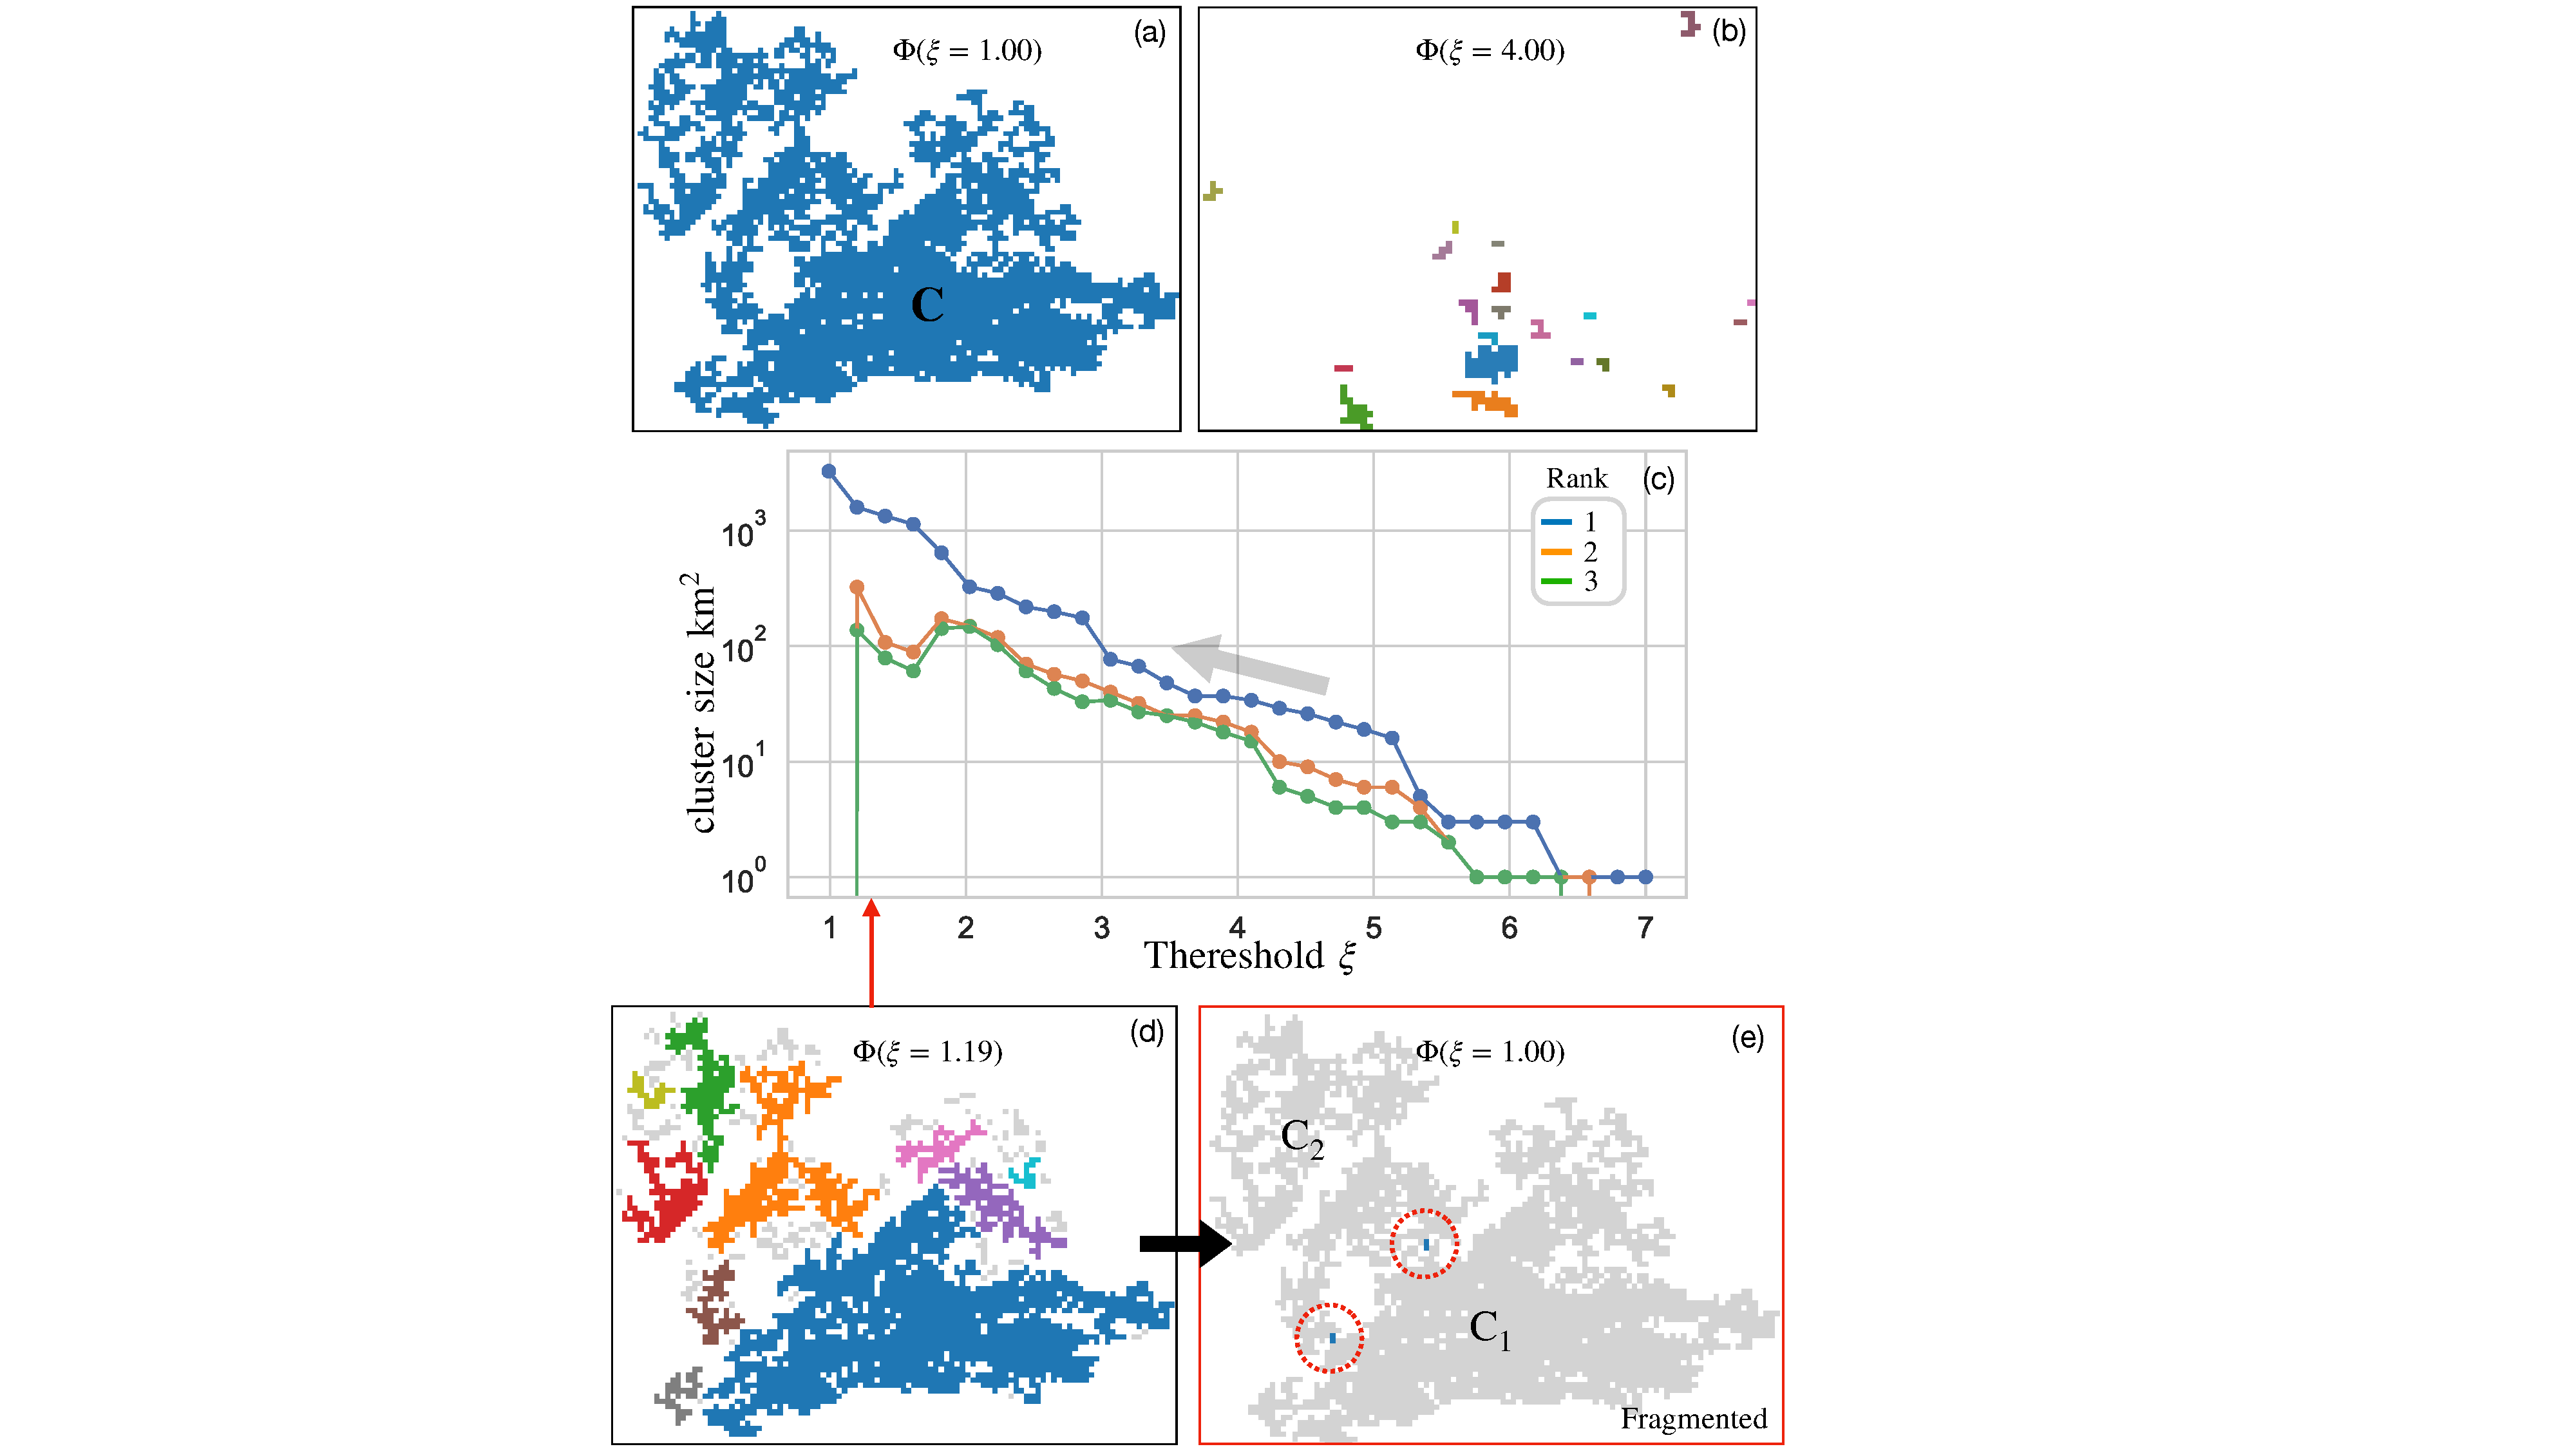
\includegraphics[scale=0.5]{chapter7/figures/figure1-frag-method.pdf}
    \caption{
    A graphical illustration of the algorithm developed to fragment $R_0$-clusters.  
    (a) The largest cluster, denoted by $\mathbf{C}$, is shown inside an arbitrary domain at resolution $3\mathrm{km} \times 3 \mathrm{km}$ and infectiviy $\beta^*=450$ for the model $\phi_1$-ga.
    Applying the threshold function $\Phi$ at $\xi=1$ recovers the $\mathbf{C}$ exactly because all patches are above the threshold $R_0=1$.
    (b) Applying the threshold function $\Phi$ at $\xi=4$ yields a low-density map with sparsely distributed clusters, as few patches surpass $R_0\geq 4$. 
    (c) The top three largest clusters, by area $\mathrm{km^2}$, are shown as a function of $\xi$.
    (d) At specific values of $\xi$, some sub-clusters join to form larger clusters\textemdash here, the blue and orange clusters proceed to join at $\xi = 1.15$.
    (e) Connecting patches are identified when large discontinuities arise when back-stepping $\xi \rightarrow \xi -\delta \xi$, shown here by the blue pixels; removing these patches fragment the cluster $\mathbf{C}$ in $\mathbf{C_1}$ and $\mathbf{C_2}$. 
    }
    \label{fig:R0-threshold-function}
\end{figure}

Figure \ref{fig:R0-threshold-function} shows the how the function $\Phi(\xi)$ allows the identification of high priority spatial locations.
In Figure \ref{fig:R0-threshold-function}(a) we begin with a target-cluster, $\mathbf{C}$, shown in blue;
$\mathbf{C}$ is the largest cluster detected in an arbitrary $R_0$-map for the model $\phi_1$-ga and infectivity $\beta^*=450$ (as described previously in chapter \ref{ch:6-adb}).
Applying the threshold function $\Phi(\xi=1)$ recovers $\mathbf{C}$ entirely, as all patches in $\mathbf{C}$ are over the threshold.
In contrast, larger values of $\xi$ result in a lower-density map with sparsely distributed clusters, 
demonstrated by the small number of labelled clusters in Figure \ref{fig:R0-threshold-function}(b) at $\Phi(\xi=4)$.
Similarly, only one (or at most a handful) of patches populate the domain at the limiting value $\Phi(\xi=R_{max})$.

Connected component analysis (CCA) is performed at each step $\xi \in [1, R_{max}]$ in order to identify and label sub-clusters. 
At particular steps $\xi \rightarrow \xi - \delta\xi$ (i.e. back-stepping), $\mathbf{C}$ will begin to form when distinct sub-clusters\footnote{
It is possible that three or more sub-clusters suddenly connect to form $\mathbf{C}$ in the same step; 
these complexities are taken into account by the algorithm.} 
 (e.g. $\mathbf{C_1}$ and $\mathbf{C_2}$) suddenly connect when certain critical links become non-zero\textemdash
analogous to the formation of a spanning cluster opening up in a percolation. 
Figure \ref{fig:R0-threshold-function}(d) depicts a scenario with a number of disconnected sub-clusters at $\xi=1.19$ that merge together at $\xi=1.15$.
The well-known `binary dilation' operator \cite{liang1989erosion, 23111, nachtegael2001connections} was used to detect all patches that become non-zero and bridge sub-clusters, as elaborated in \textcolor{red}{appendix X}.
Henceforth, `connecting patches' refer to patches that connect sub-clusters in a discontinuity step.

When $\mathbf{C_1}$ and $\mathbf{C_2}$ abruptly merge to form the basis of $\mathbf{C}$, a significant discontinuous jump in cluster size is detected. 
All spatial locations $(i,j)$ which bridge the gap between $\mathbf{C_1}$ and $\mathbf{C_2}$ are then identified and removed by taking $R_0$ below the threshold.
Figure \ref{fig:R0-threshold-function}(e) shows two singular patches in blue (and highlighted in red) that if taken below $R_0=1$,
would fragment $\mathbf{C}$ into two sub-clusters $\mathbf{C_1}$ and $\mathbf{C_2}$.
Successive steps through $\xi$ continue until $\xi=1$.
For each discontinuity event, connecting patches are detected and removed from the system,
thus preventing $\mathbf{C_1}$ and $\mathbf{C_2}$ from merging over $\xi \in [1, R_{max}]$.
In this manner, the target-cluster $\mathbf{C}$ is fragmented into two separate sub-clusters. 
As we can see, connectedness within the domain can depend on a small number of patches.

\subsection{Iterative cluster fragmentation}
\label{sec:fragmentation-method-2}

Each $R_0$-cluster can be iteratively fragmented $N$ times to produce a set of disconnected sub-clusters, 
where, on average, each fragmentation iteration produces $N+1$ sub-divided clusters.
Figure \ref{fig:iterative-fragmentations} demonstrates the iterative process for the example cluster $\mathbf{C}$ from Figure \ref{fig:R0-threshold-function}(a).
During first iteration the target cluster $\mathbf{C}$ is fragmented into $\mathbf{C_1}$ and $\mathbf{C_2}$, shown respectively in Figure \ref{fig:iterative-fragmentations}(a) as orange and blue.
After each iteration, sub-clusters are ranked according to the area they cover, the next iteration proceeds by targeting the largest sub-cluster;
this is illustrated in Figure \ref{fig:iterative-fragmentations}(b) when $\mathbf{C_1}$ is targeted during the next iteration at $N=2$, producing a third disconnected sub-cluster ($\mathbf{C_3}$) shown in green. 
The process is then repeated $N=10$ times to produce $11$ disconnected fragments in Figure \ref{fig:iterative-fragmentations}(c).

\begin{figure}
    \centering
    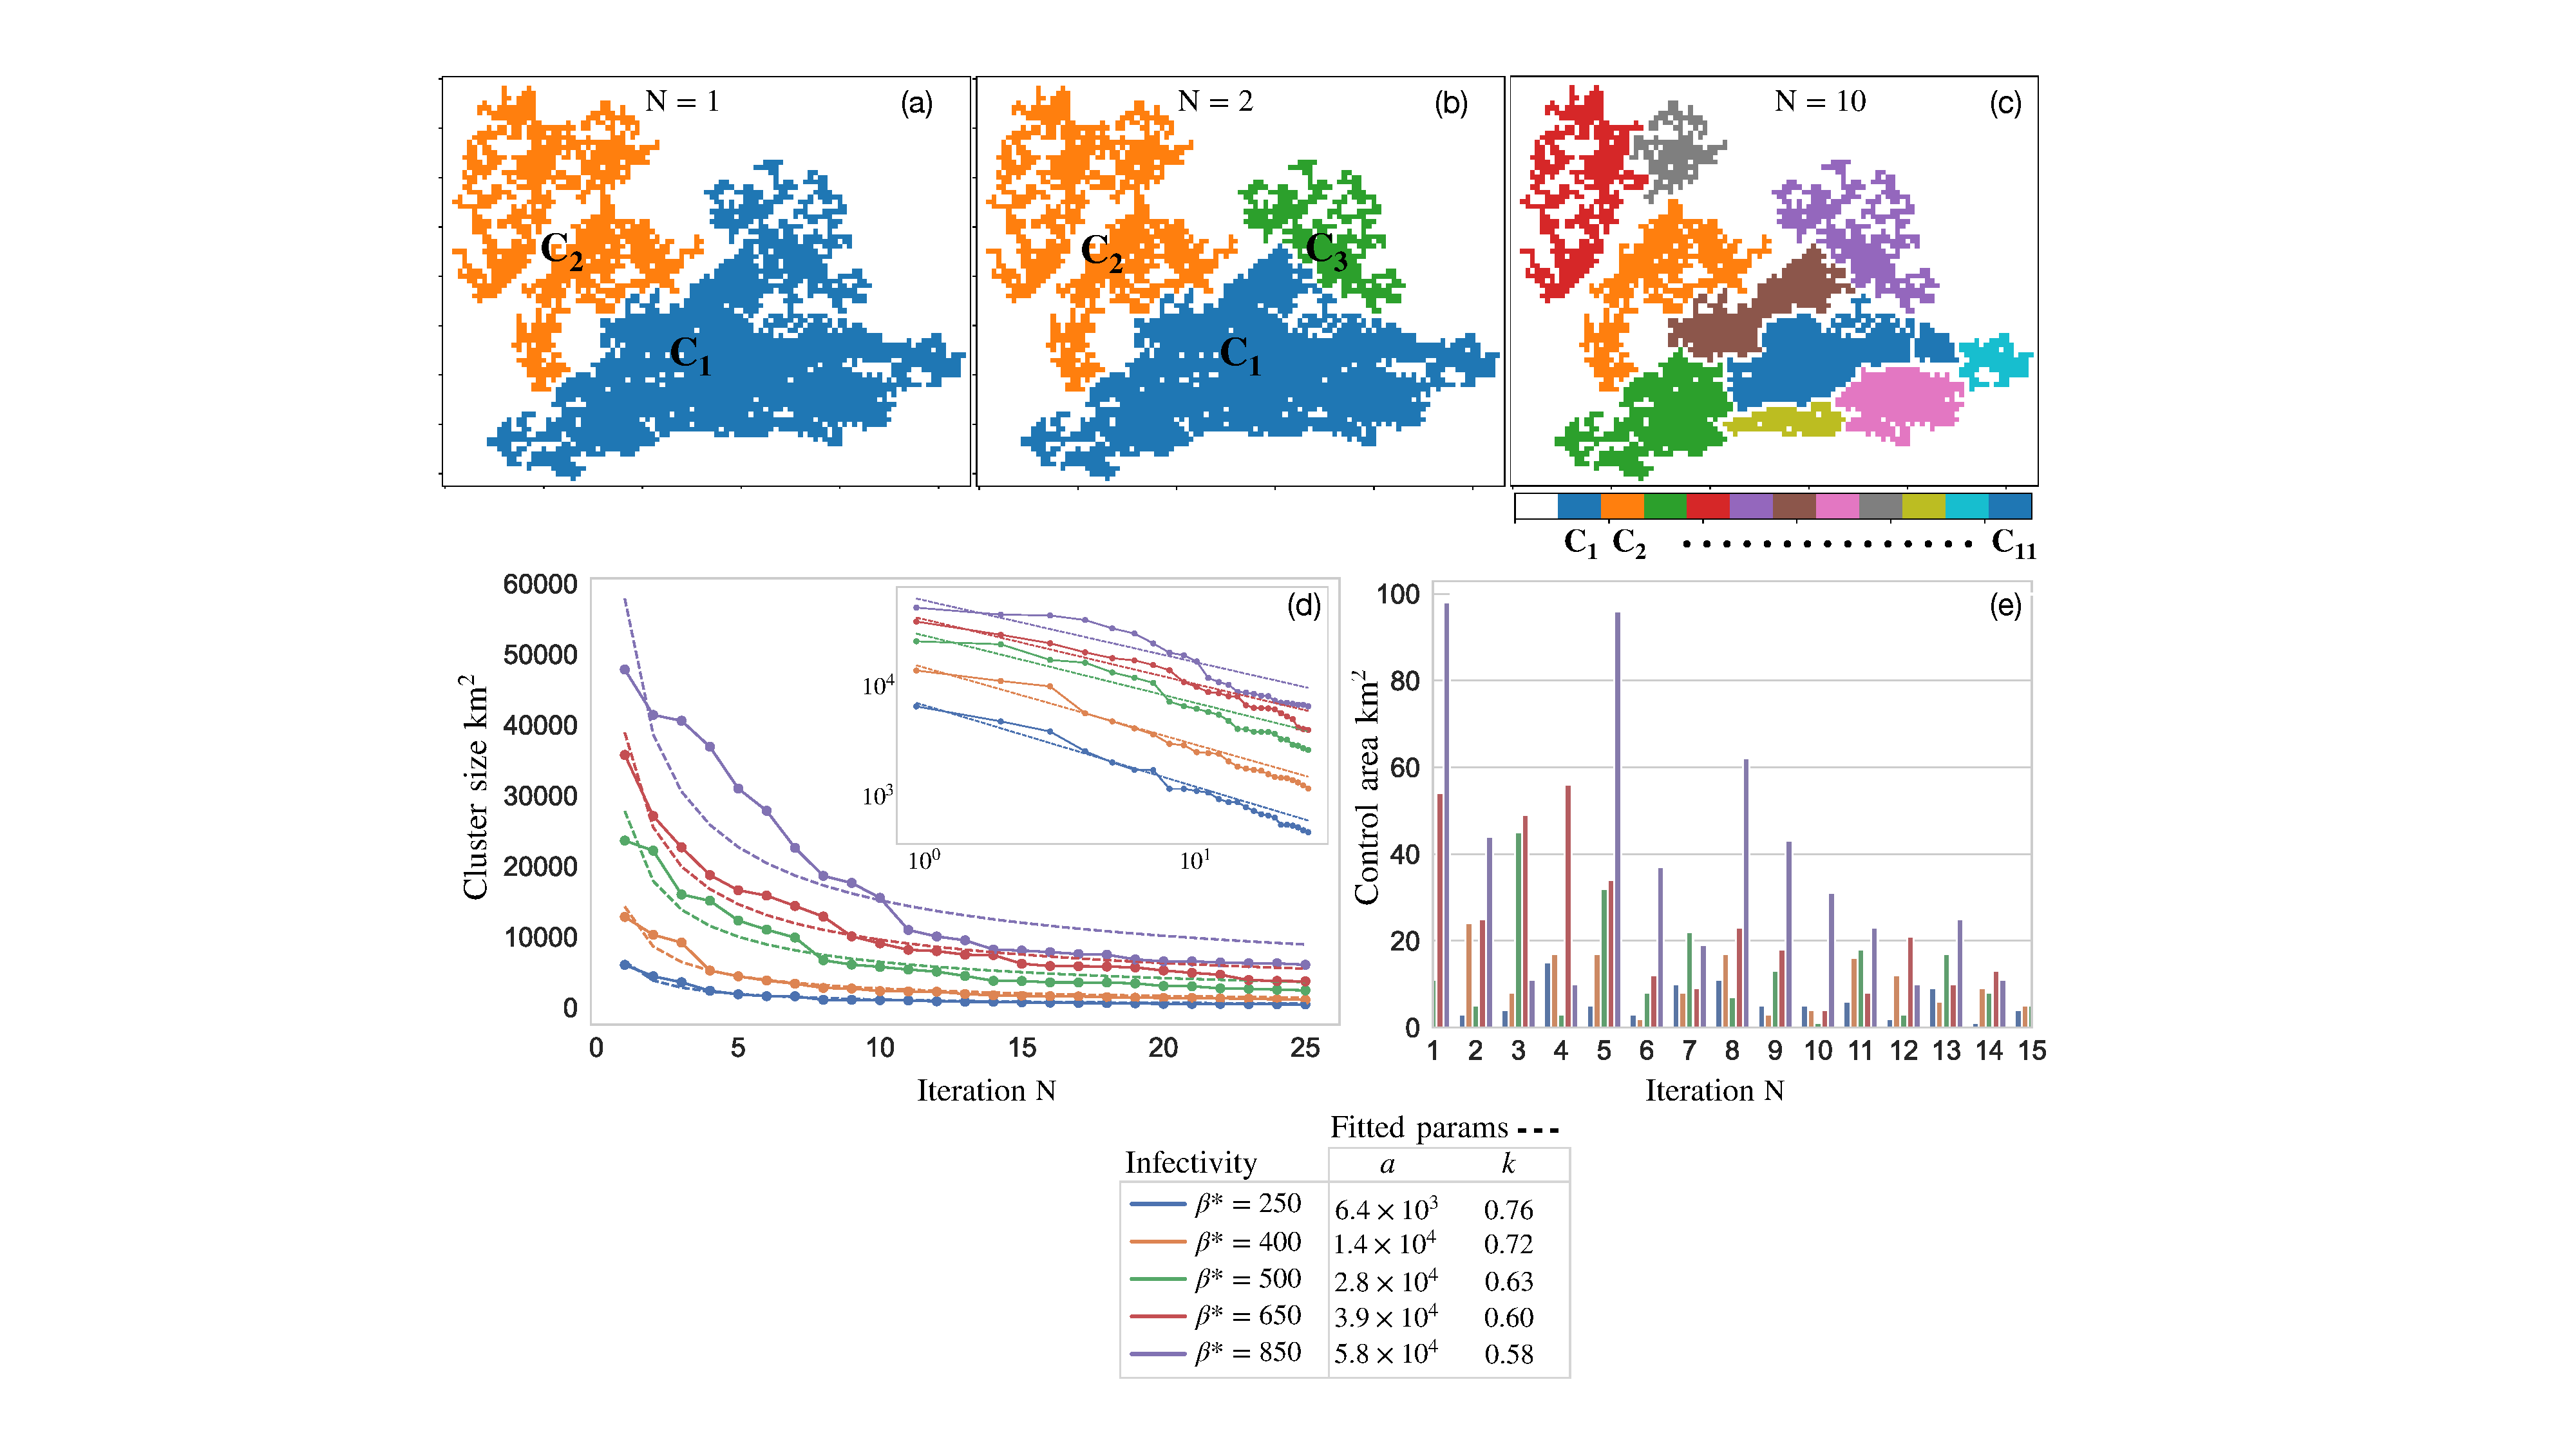
\includegraphics[scale=0.41]{chapter7/figures/figure2-Iiterative-frag.pdf}
    \caption{
    The fragmentation algorithm is shown as an iterative process. 
    (a) The example cluster ($\mathbf{C}$) is fragmented into two sub-clusters ($\mathbf{C_1}$ and $\mathbf{C_2}$) during the first iteration of the algorithm.
    (b) During the next iteration, the largest sub-cluster $\mathbf{C_1}$ is targeted to produce an additional cluster fragment, denoted here by $\mathbf{C_3}$ in green.
    (c) The process is iteratively repeated $N=10$ times to produce $11$ sub-dived clusters.
    (d) The sub-cluster size reductions are plotted for $25$ iterations of the algorithm over a range of infectivity parameters;  
    approximately, size-reduction follows an inverse power law, as indicated by the corresponding fitted dashed lines.
    Lower infectivity parameters correlate to an efficient fragmentation in contrast to higher $\beta^*$ values\textemdash suggested by the logarithmic inset plot.
    (e) The area of connecting patches, or `control area', is plotted against the iteration\textemdash truncated to $15$. 
    Generally, the number of connecting patches increases with infectivity and decrease with iteration.
    }
    \label{fig:iterative-fragmentations}
\end{figure}

Figure \ref{fig:iterative-fragmentations}(d) shows the sub-cluster size reductions for $N=25$ iterations and a number of different infectivity parameters.
For all infectivity parameters considered, the largest sub-cluster continually decreased for each iteration of fragmentation.
Moreover, cluster size reductions occurred more rapidly at first and slowed down as $N\rightarrow 25$.
Sub-cluster size reductions were fitted to an inverse power law of the form $f(x) = ax^{-k}$, shown by the corresponding colored dashed lines in Figure \ref{fig:iterative-fragmentations}(d).
Fitted parameter values of $a$ and $k$ reflect the initial cluster size and rate of decrease, respectively. 
Higher infectivity parameters fit a larger constant $a$ and a smaller exponent $k$, indicated in the legend.
Therefore, the fragmentation process becomes progressively inefficient as $\beta^*$ increases,
demonstrated most clearly by comparing the gradient of the purple and blue lines in the logarithmic inset axes\footnote{
Additionally, fragmentation was tested alongside the $2^{nd}$ and $3^{rd}$ largest $R_0$-clusters (not shown); 
for each value of $\beta^*$, $a$ and $k$ compared similarly to the $2^{nd}$ and $3^{rd}$ largest ranked clusters.}.

Lastly, Figure \ref{fig:iterative-fragmentations}(e) shows the corresponding number of connecting patches, or `control area', identified over each $\beta^*$ value and iteration.
The number of removed patches tends to decrease with iteration\textemdash most likely due to the smaller areas involved\textemdash and increase with infectivity.
For example, when $\beta^*=850$, Figure \ref{fig:iterative-fragmentations}(e) shows a control area on the order of $100\mathrm{km^2}$,
arguably, treating a spatial extent of this magnitude would be exceedingly challenging in practice.
Thus, when $\beta^*$ becomes high, it is clear to see a limitation in the framework.
In the next section, we outline a potential framework for using cluster fragmentation as a means to achieve `regional containment'.

\section{Towards regional containment (unfinished)}
\label{sec:towards-regional-control}

Regional containment can be tested as an epidemic control strategy by considering hypothetical outbreaks from various epicentres. 
Figure \ref{fig:scenario-expo} demonstrates containment for a single epicenter marked by the black cross\textemdash 
located inside the same target cluster shown in Figures \ref{fig:R0-threshold-function} and \ref{fig:iterative-fragmentations}.
We can achieve epidemic containment in several ways, as alluded to by Figure \ref{fig:scenario-expo}.
The connecting patches (identified over $N=25$ fragmentation iterations) can be combined in many ways to define different boundaries around the epicentre.
For example, Figure \ref{fig:scenario-expo}(a) defines a boundary by considering connecting patches determined in the $1^{st}, 3^{rd}, 7^{th}$ and $8^{th}$ iterations, shown in red.
The boundary then defines a confining sub-cluster around the epicentre; 
in theory, light-grey patches remain disconnected and susceptible whilst the dark grey patches are removed/at-risk.

A simple notion of `control-payoff' can be described by the ratio $N_{S}/(N_{R}\times N_{C})$,
where $N_S$, $N_{R}$ and $N_{C}$ are the number of patches that remain susceptible, become removed and are targeted for control, respectively.
We have efficient containment when the number of `saved' patches is high and the number of patches removed and controlled is low.
For the remainder of this chapter, the notion of control is kept generic and undefined\textemdash
although it typically involves either the culling or biological treatment of infected hosts.
Furthermore, resources to control the pathogen are finite and depend on governmental budgets.
With more work, we may be able to compute a limit on $N_{C}$ and perform a more sophisticated analysis.
In a similar vein, $N_R$ paints the simple picture of patches becoming removed/at-risk; 
in reality, the number of patches at risk of removal would be more complicated and subject to LDD and stochastic below-threshold outbreaks. 
However, with no expressed limit on $N_{C}$ and a simple notion of $N_S$ we continue with a theoretic investigation.

\begin{figure}
    \centering
    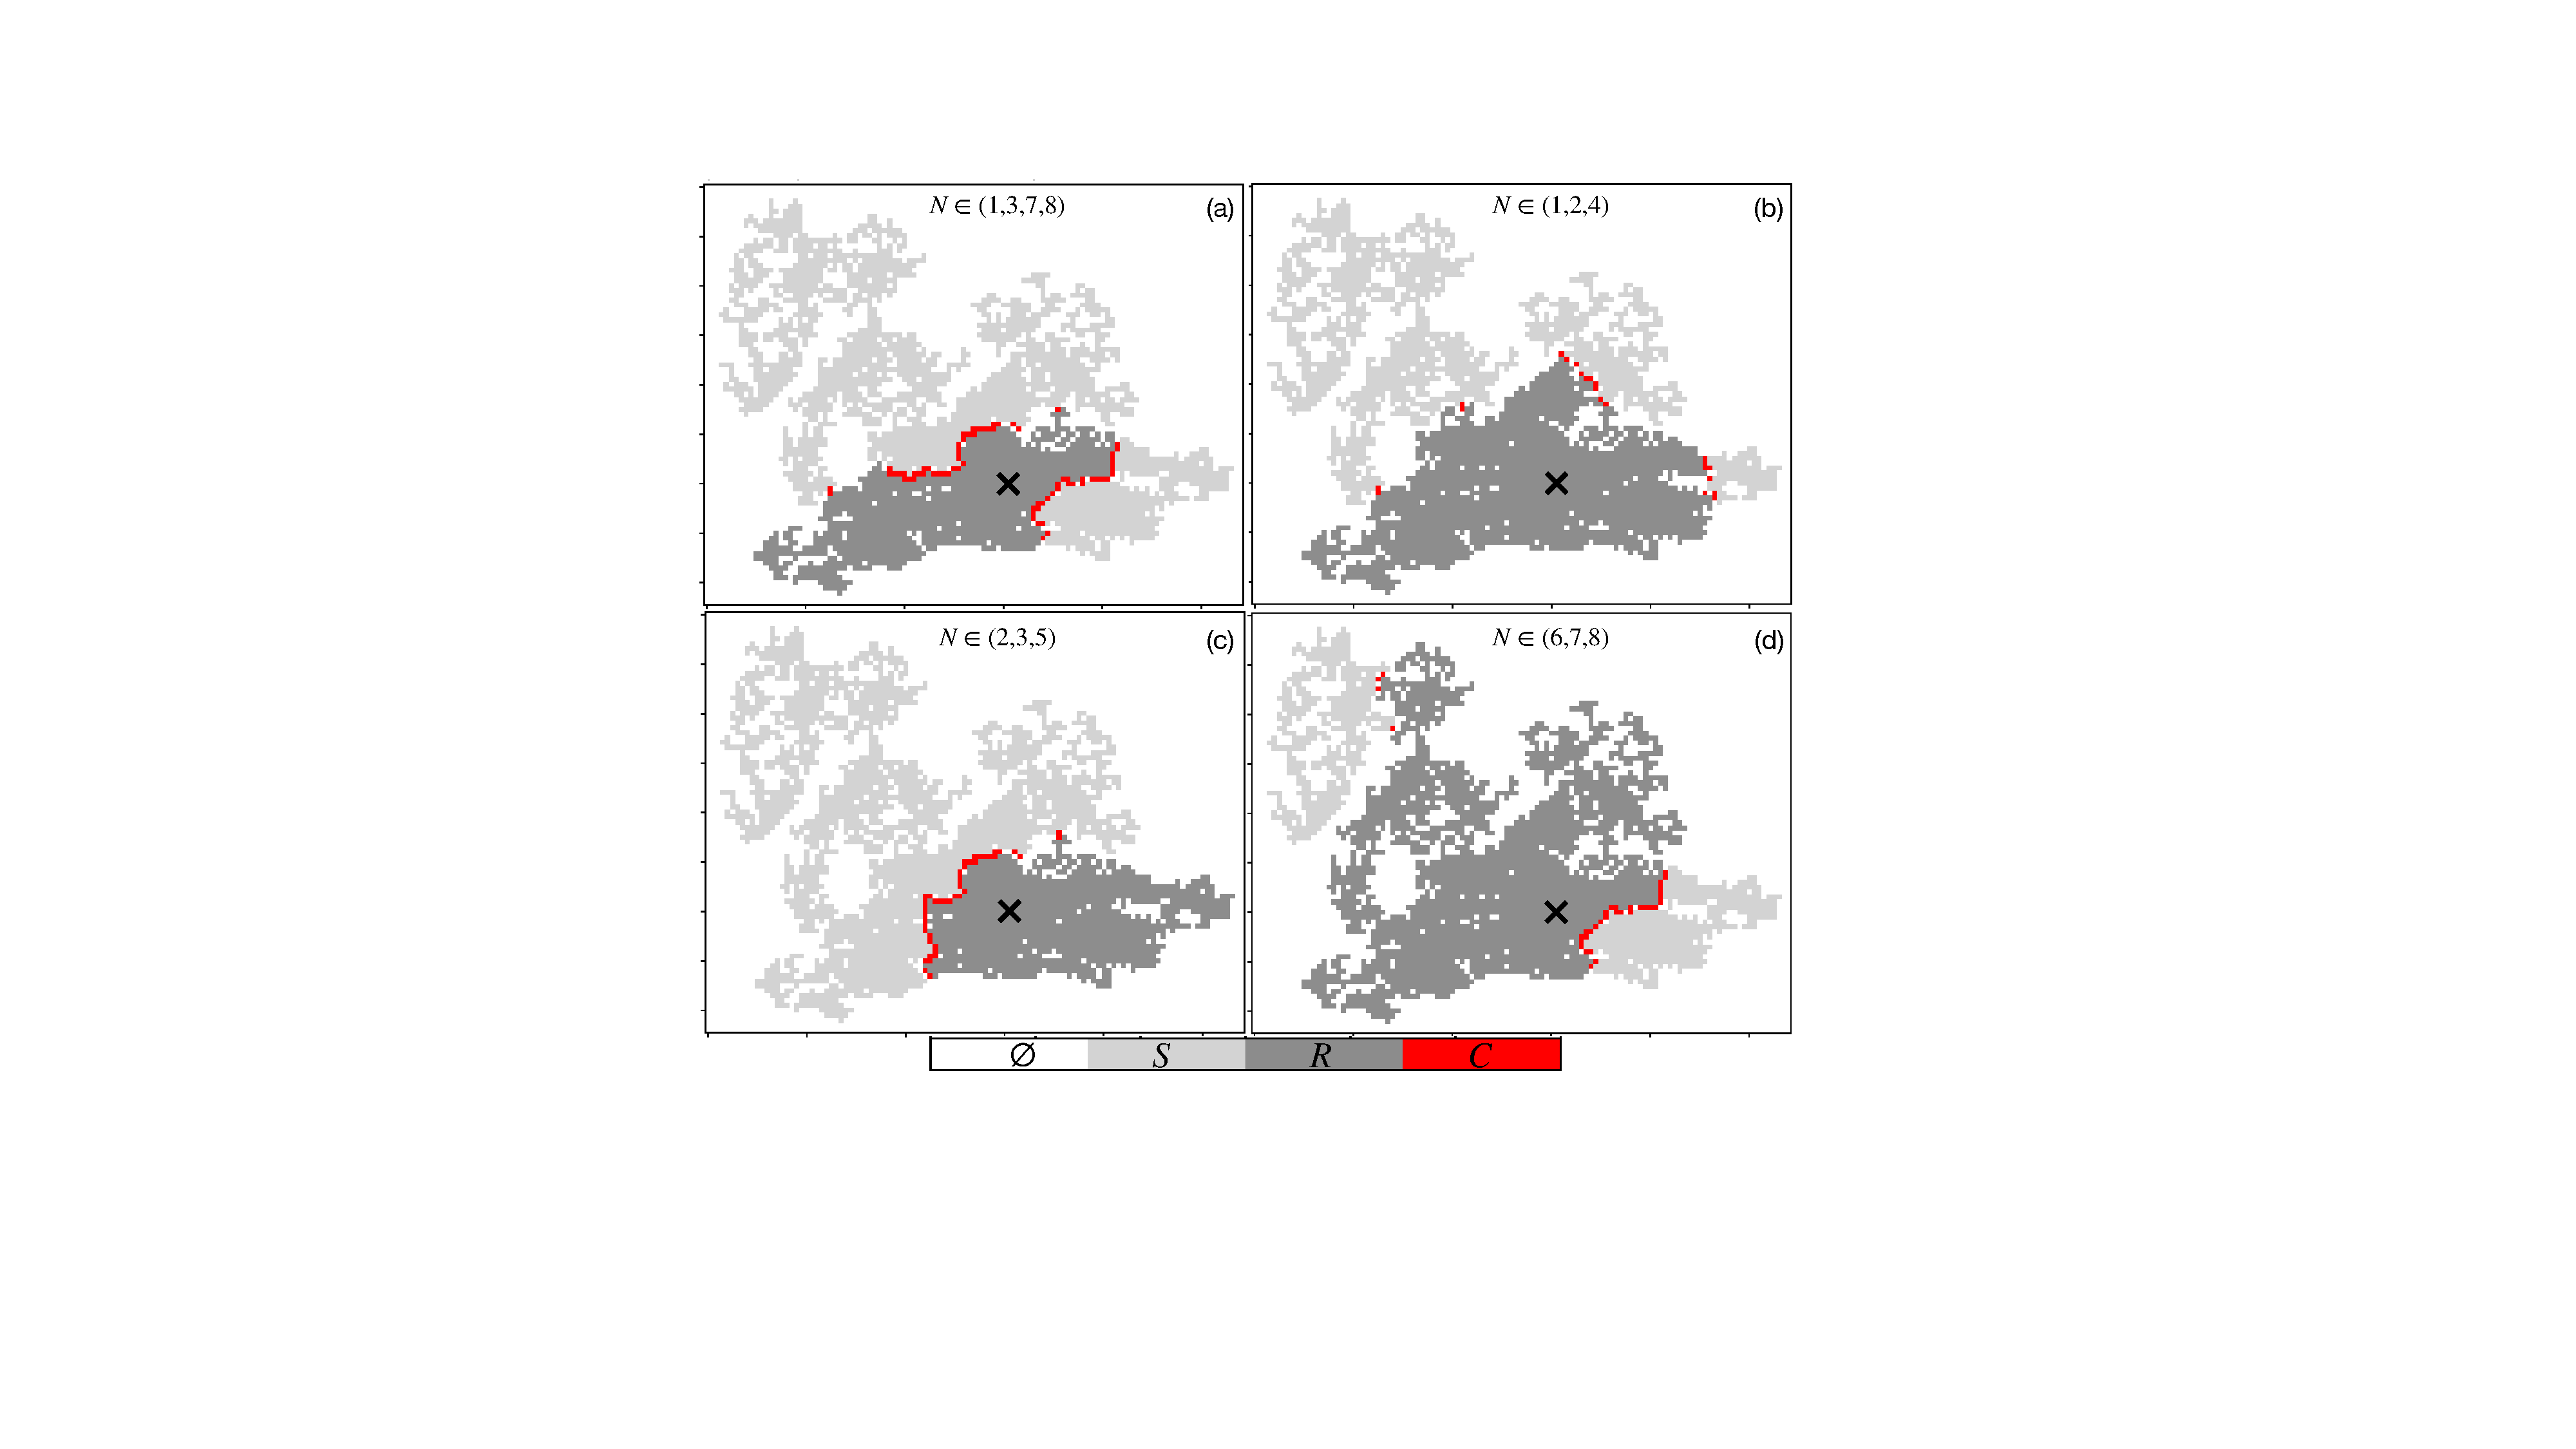
\includegraphics[scale=0.575]{chapter7/figures/figure3-scenario-test.pdf}
    \caption{
    A variety of different control choices are possible for each epicentre, based on the landscape-level host aggregation. 
    Here, the algorithm recursively fragments the target cluster $\mathbf{C}$ through $N=25$ iterations, 
    then different combinations of connecting patches can be used to contain the outbreak in a variety of ways.
    Panels (a-d) represent a small sample of control scenarios for an arbitrary epicentre marked by the central black cross.
    Red patches indicate where landscape-level control $C$ should be targeted to contain the epidemic.
    Light grey patches remain susceptible ($S$) whilst dark grey parches are assumed removed/at-risk, denoted by $R$.
    In practice, every possible control scenario is assessed against every possible epicentre.
     }
    \label{fig:scenario-expo}
\end{figure}

Lastly, it is worthwhile to describe some edge cases and complexities that arise when determining containment scenarios.
Suppose that containment is detected about an epicentre by combining the connecting patches identified in two arbitrary iterations $N_i$ and $N_j$.
In this scenario, some patches from $N_i$ and $N_j$ may be located away from the containing sub-clusters boundary, i.e. in distant (non-bounding) locations.
Thus, irrelevant (non-connecting) patches were identified by employing the binary dilation operator; in this way, only patches neighbouring the confining sub-clusters perimeter contribute to $N_C$.
Moreover, combinations of connecting-patch iterations that failed to define a confining sub-cluster about the epicentre must be ruled out from the analysis.

\newpage

\subsection{Results: control payoff}

Scenarios tests employ a variety of different epicentres to consider Landscape-level epidemic containment in Great Britain.
Moreover, the sub-cluster centre of mass (COM) defines an epicentre, i.e. we compute the COM for each sub-cluster produced from $N=20$ iterations of target-cluster fragmentation. 
As before, `target cluster' refers to the largest dominating cluster detected in the $R_0$ map for each $\beta$-valued domain.
Containment scenarios can then be determined for each epicenter\textemdash as described above.
The payoff ratios were then ranked according to the payoff ratio $N_S/ (N_R\times N_C)$, as shown in Figure \ref{fig:payoff-efficiency}\textemdash 
all panels consider the model $\phi_1$-ga resolved to $\mathrm{5 km \times 5 km}$ sized patches.

Figure \ref{fig:payoff-efficiency}(a) presents the top $25$ epidemic containment scenarios over a range of infectiviy parameters in the interval $\beta^* \in [0, 1000]$. 
The reader is referred back to chapter \ref{ch:6-adb} (i.e. Figures \ref{fig:R0-map-generation} and \ref{fig:gaussian-clustering}) for background information on cluster size with infectiviy $\beta^*$.
Beyond $\beta^*=200$, each value of infectivity involved a large number of containment scenarios, i.e. typically between $10^3-10^4$ containment scenarios per $\beta^*$ parameter.
The payoff ratio starts small with low infectivity values and begins to peak before dropping off. 
The control payoff is low for low values of $\beta^*$ since the number of trees saved is generally lower on account of small susceptible clusters.
Figure \ref{fig:payoff-efficiency}(a) therefore indicates that this strategy of control is not desirable for pathogens with low infectivities.
For exceptionally high values of $\beta^*$, a small number of high-valued payoff ratios are plotted in the shaded region Figure \ref{fig:payoff-efficiency}(a); 
this represents a limitation when using the payoff ratio as defined in this chapter\textemdash \textcolor{red}{see Appendix X for a graphical explanation}.

Interestingly, Figure \ref{fig:payoff-efficiency}(a) suggests that regional epidemic containment is most efficient over a specific parameter regime,
since the highest payoff scenarios occur in the interval $\beta^* \in [400, 600]$.
Although, these are preliminary indications. 
As section \ref{sec:gaussian-r0-clustering} demonstrated, nearest-neighbour structuring elements do not scale with changes landscape-level resolution.
Given that Figure \ref{fig:payoff-efficiency}(a) is based on $\phi_1$-ga at the resolution $5\mathrm{km} \times 5\mathrm{km}$, the results presented by Figure \ref{fig:payoff-efficiency}(a)
are likely to change if containment scenarios are computed with smaller patch sizes.
Although Figure \ref{fig:payoff-efficiency}(a) demonstrates an important observation, 
more work is needed to be confident that regional containment is most effective over the interval $\beta^* \in [400, 600]$.

Figure \ref{fig:payoff-efficiency}(b) shows the complete list of scenario tests for $\beta^*=500$, the infectivity that registered the highest control payoff.
The number saved patches that remain in $S$ (i.e, $N_S$) is plotted against $N_R \times N_C$.
The upper and right-hand marginal plots show the corresponding probability density functions for $N_S$ and $N_R \times N_C$.
Each PDF shows a skewed distribution, with most scenarios involving a smaller value of $N_S$ and $N_R \times N_C$.
Of the $3850$ containment scenarios, a small number of high performing tests populate the bottom right-hand quadrant, when $N_S$ is large and $N_R \times N_C$ is low;
this region represents viable scenarios where containment is most efficient i.e. the right and left-hand distribution tails when $N_S$ is large and $N_R \times N_C$ is small.

Figures \ref{fig:payoff-efficiency}(c-e) show three scenarios of interest, orange and blue clusters depict removed/at-risk and susceptible/saved patches, respectively. 
Red crosses indicate where the control should be focused to achieve containment. 
The targeted control patches in Figure \ref{fig:payoff-efficiency}(c) resemble those identified previously in Figure \ref{fig:R0-threshold-function}(e), albeit this time for a higher $\beta^*$-valued domain at a lower landscape-level resolution.
Desirably, observing connecting patches in approximately the same location for different infectivity values suggests that some patches may be important for control at various epidemic scales.
Moreover, Figure \ref{fig:payoff-efficiency}(c) hints toward there being similarities at and different resolutions\textemdash the concern mentioned above.

\begin{landscape}
\begin{figure}
    \centering
    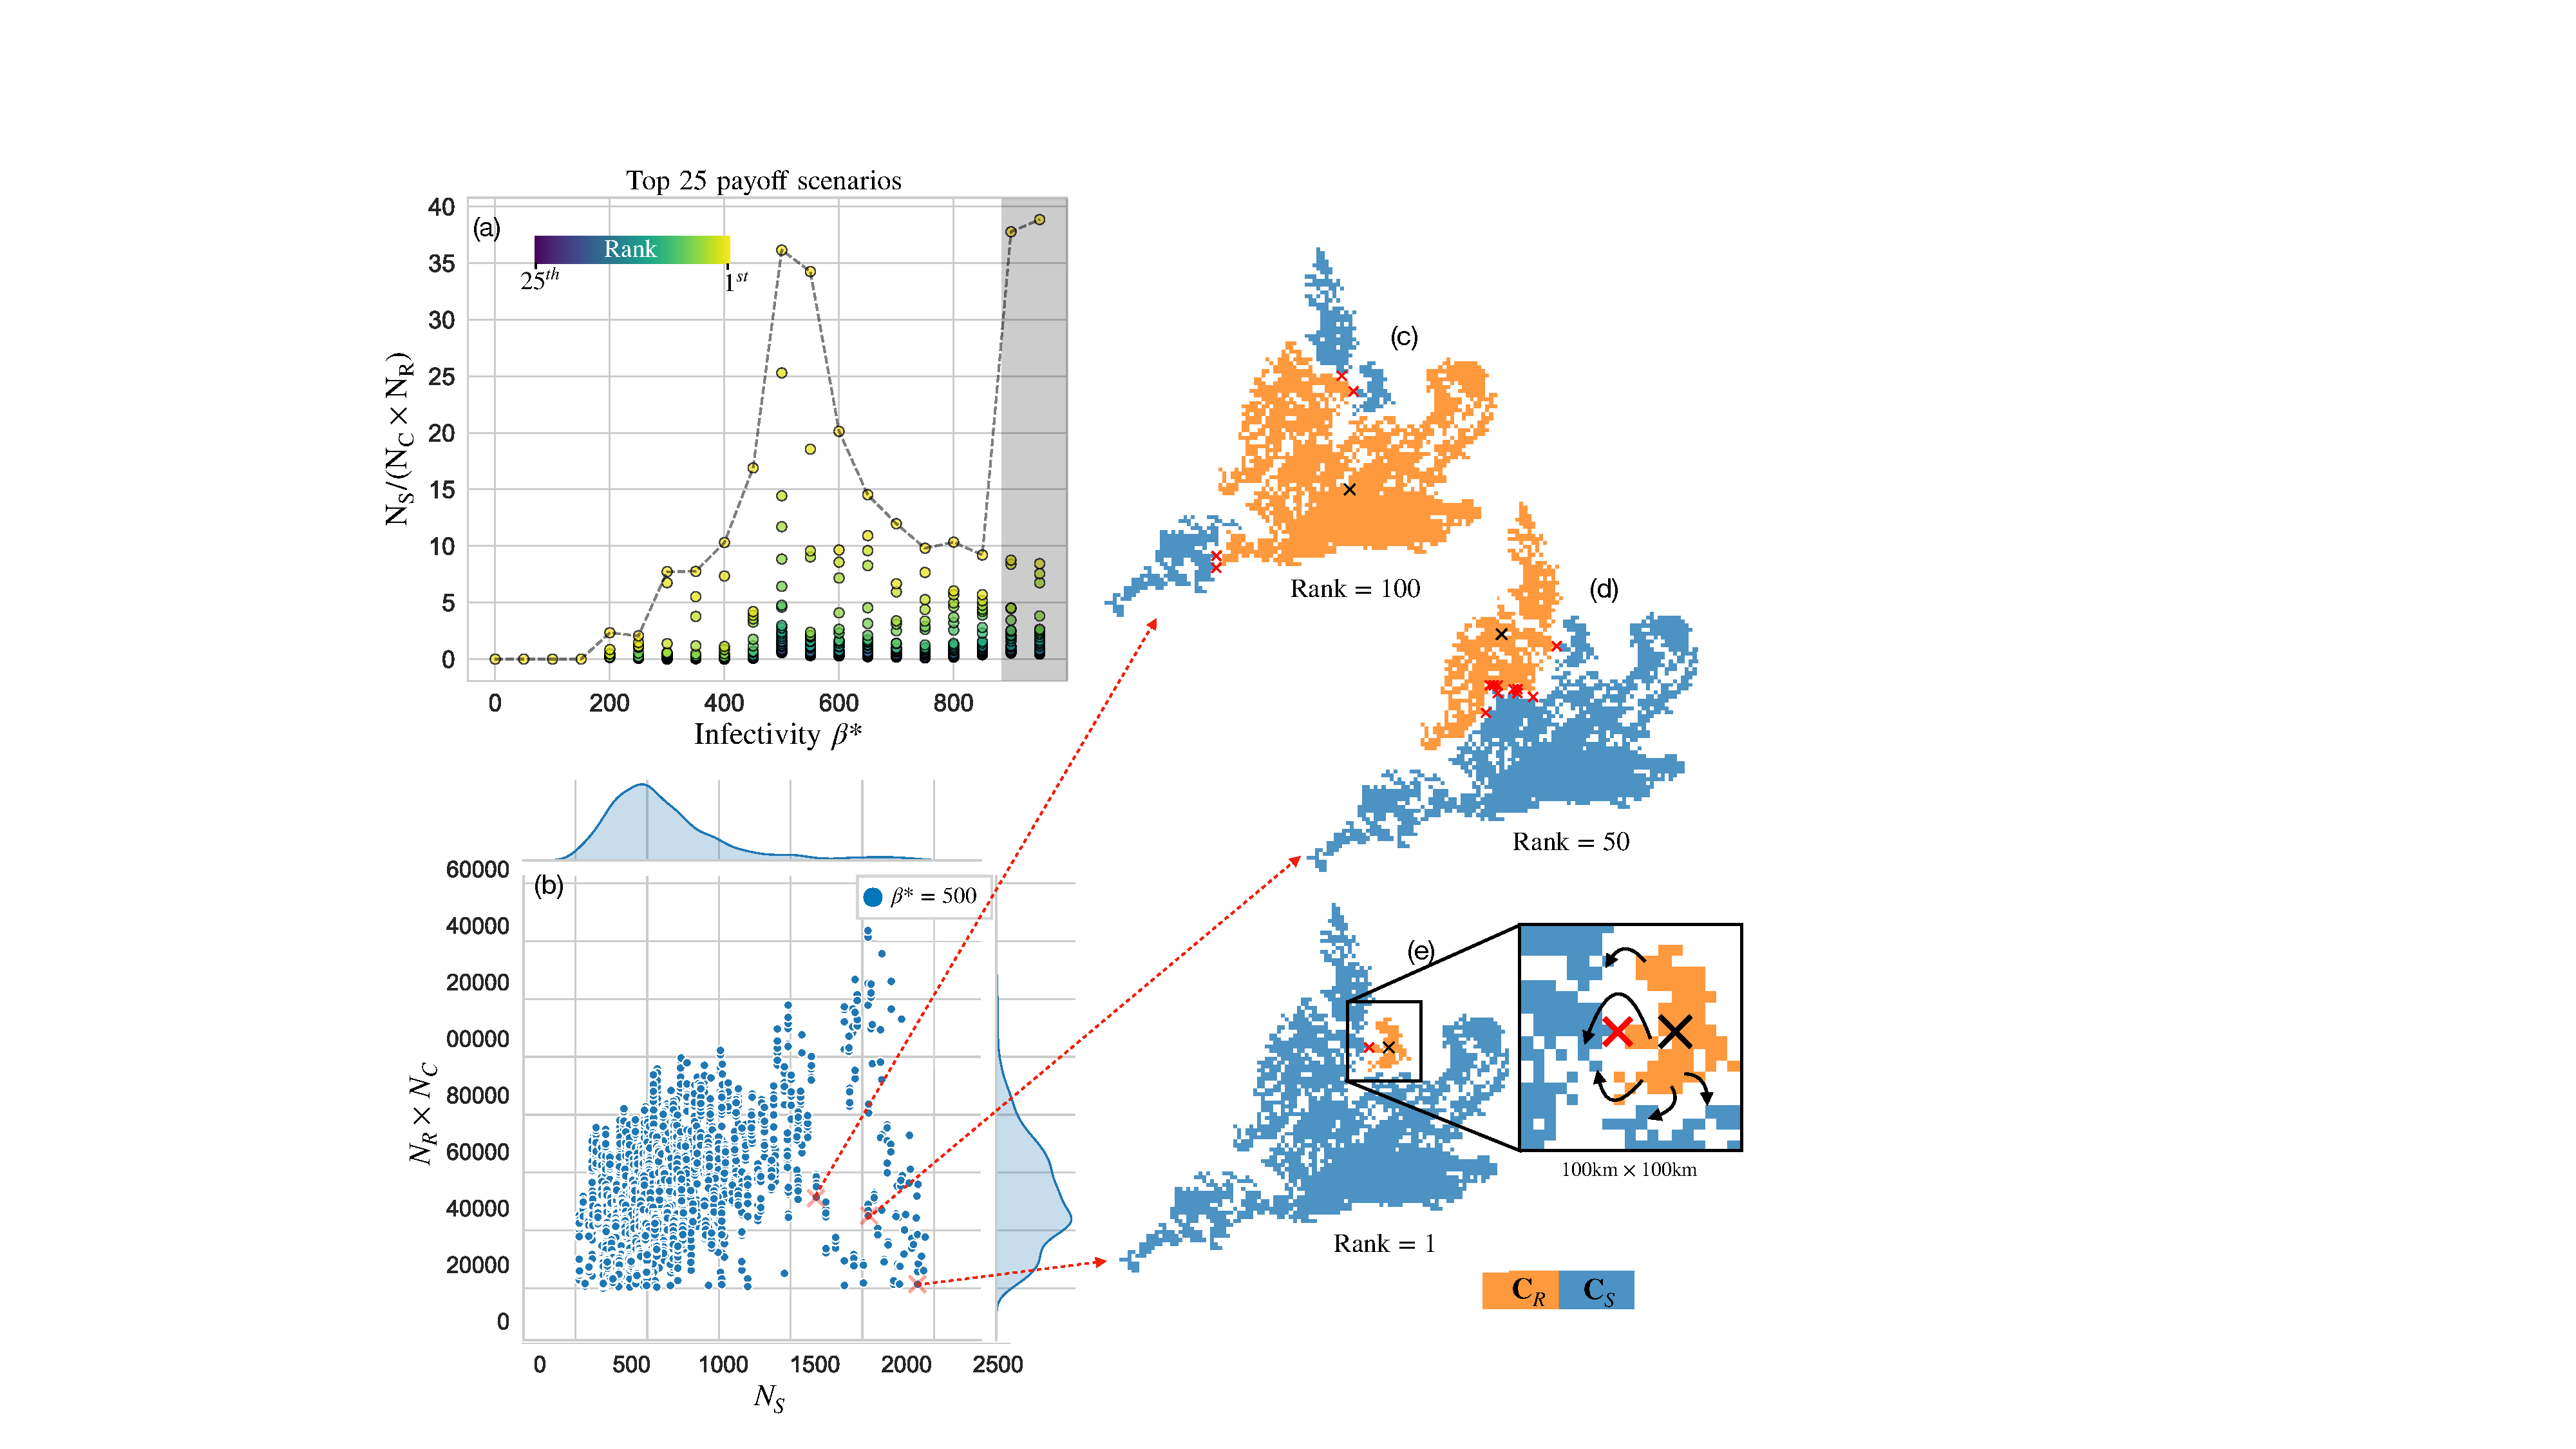
\includegraphics[scale=0.47]{chapter7/figures/figure4-scenario-payoff.pdf}
    \caption{The control `payoff' is accessed by comparing the number of patches that remain susceptible ($N_S$) against the number of patches removed ($N_R$) and controlled ($N_C$).
             (a) The payoff ratio $N_S / (N_R \times N_C)$ is plotted against the infectiviy parameter $\beta^*$ for the top $25$ highest payoff scenarios.
             (b) The complete list of (3850) different scenario tests are plotted for the highest payoff infectivity parameter $\beta^*=500$; the lower right-hand quadrant defines the most efficient control scenarios.
             (c-e) Spatial plots that show three hypothetical scenarios from panel (b). 
             Blue and orange clusters outline patches that remain susceptible and become removed, respectively.
             (f-g) Probability density functions for $N_S$ and $N_R \times N_C$ are plotted over the sample of shown infectivity parameters.
             }
    \label{fig:payoff-efficiency}
\end{figure}
\end{landscape}

Figure \ref{fig:payoff-efficiency}(c) reveals the highest payoff result for $\beta^*=500$.
In this scenario, the epicentre lies close to the Eastern coastline (Skegness), 
and the control area is located slightly inland (approximately between Lincoln and Sheffield).
The zoomed inset highlights a single $\mathrm{5km \times 5 km}$ patch, and control saves the vast majority of GB from infection.
This scenario is no doubt idealistic and unlikely to be realised in a real-life outbreak.
In a real-life outbreak, epicentres are unlikely to be so conveniently located about the coastline.
Furthermore, detecting and controlling the pathogen remains difficult before it spreads to distant (and more centralised) locations.
Nevertheless, Figure \ref{fig:payoff-efficiency}(c) reinforces the intuitive notion that epicentres around edge positions are contained efficiently.
The inset highlights where pathogen dispersal might jump between clusters, indicated by the curved arrows.
Although wind-dispersed secondary infections are likely rare over these spatial scales ($5$-$20\mathrm{km}$), they are nevertheless thought possible for fungal spores \cite{grosdidier2018tracking};
the analysis presented here neglect these complexities, which requires further investigation.

The last spatial plot, Figure \ref{fig:payoff-efficiency}(d), depicts a more likely scenario with a centrally located focus.
Most of GB remains at risk, yet some Northern and Southern regions surrounding the target cluster remain protected from the pathogen.
If the disease has not yet reached the connecting patches (identified by the red crosses), Figure \ref{fig:payoff-efficiency}(d) indicates that regional containment might be attempted alongside targeting a disease wave-front \cite{large-scale-control}, or more local-scale pathogen eradication \cite{WEBIDEMICS}. 
Although, ultimately, more work is needed to assess the efficacy and possibility of halting/slowing the spread.

Figures \ref{fig:payoff-efficiency}(f-g) show the probability density functions associated with $N_S$ and $N_R \times N_C$ for the infectiviy values shown.
Generally, higher infectivity parameters skew the distribution of $N_S$ towards higher values because the number of patches available to save generally grows alongside the overall cluster size.
Similarly, the distributions of $N_R \times N_C$ also becomes skewed toward the right, indicating that most control scenarios become progressively inefficient as infectivity grows.
However, landscape-level control is possible when scenarios occupy the right and left-hand distribution tails of $N_S$ and $N_R \times N_C$.

\section{Chapter summary}

This chapter outlined a conceptual strategy of landscape-level control, targeting a pathogens local wind-dispersal mechanism.
The strategy preferentially controls the pathogen through identified patches throughout the host population.
If taken below the epidemic threshold, $R_0$-cluster fragmentation could be achieved along with an idealistic `regional containment'.
Although, the utility, efficiency and practicality of real-life implementation remain unproven, given that the effects of LDD (beyond $5\mathrm{km}$) was neglected and spores likely disperse over large distances, e.g. from mainland Europe to Great Britain \cite{freer2017tree, wylder2018evidence}.
Nevertheless, the results of section \ref{sec:cast-study-jump-patches} provide indications that pathogen dispersal might, at worst, be slowed by performing patch-level density reductions;
in the best-case scenario, policymakers and forest managers might gain vital time to respond to the threat of invasion and tree populations provided with crucial recovery time.

\textcolor{red}{
Section \ref{sec:cast-study-jump-patches} demonstrated that density reductions between intermediary patches might be a viable option of epidemic control, according to the model of $SEIR$ model of ADB.
This method contrasts with other small-scale control strategies, which typically consider a risk-based cull-radius or identify high priority hosts about known sources of infection.
Epidemic control in the Gaussian-based model was achieved with relative ease in comparison to the inverse power law variant;
inverse power law spread required more severe density reductions over larger spatial scales.
These results mirror contemporary concerns relating to the control of fat-tailed inverse power law dispersal kernels.}

% - read and discuss \cite{doi:10.1111/1365-2745.13383}, it references patch-to-patch connectivity dispersal length scales of ADB 

Although the control paradigm presented in this chapter was based on density reductions, in line with more traditional methods of eradication, 
the possibility of other biological control methods remains an attractive option.
Specifically, fungicide treatments \cite{hauptman2015application}...\textcolor{red}{elaborate}.
In addition, targeted epidemic control goes hand-in-hand with an understanding of which regions are infected.
Naturally, this leads to the emerging theme of monitoring and surveillance \textemdash discussed in section \ref{ch2:control-review}.
Various authors have suggested \textcolor{red}{x and y and z} lead to efficient monitoring;
however, none seem to involve the spatial arguments based on population heterogeneity presented in this chapter.
Consequently, future work could access the method of critical/connecting patch detection for enhanced landscape-level monitoring.

The algorithm constructed in section \ref{sec:fragmentation-method} presented a means to identify `connecting patches', which if taken below $R_0=1$ would fragment the cluster.
A related network paradigm has been articulated by many authors, relating to finding the optimal fragmentation of a network \textcolor{red}{CITE};
however, no such sources could be found relating to spatial, epidemic equivalent.
The algorithm described in \ref{sec:fragmentation-method} treated patches below the threshold as negligible.
Without this assumption, CCA would cease to work.
Given the possibility of stochastic below-threshold spread, future work should move towards a generalised (risk-based) scheme that factors in the presence of patches below $R_0=1$;
in such a scheme, we may ultimately question the choice of CCA due to its binary nature.

% - \cite{mcleish2021structuring} <-- discuss 

% The article published by \cite{time-varying-infectivity} indicates the possibility of \textit{preferentially} controlling an area based on the final-sized epidemic. 
% It goes without saying that areas of land that have the largest final sized epidemic are likely the most density populated. 
% However, we outline the possibility it might be more beneficial to preferentially control an area based on its spatial location and how it couples to to neighbouring areas.

% genetic tolerance is currently the only viable strategy of control\cite{kosawang2018fungal}

% Crucially, future work will involve integrating LDD mechanisms into the model in order to understand the relative importance long vs local distance dispersal. We may speculate about the relative importance looking at figure x, whereby the maximum distance spread in season due to local-scale spread is xm/year, in stark contrast from the observed spread of 40-60km/yr.

% We cannot overstate the importance of LDD, and it is hard to say the degree to which targeting the local dispersal mechanism alone will inhibit the spread. We will revisit this question in future work, however, we contend that preferentially targeting diseased trees based on spatial location.....could help control epidemics with greater efficacy. 

% We may speculate how our result could aid the effort of choosing where to re-plant ash stands genetically engineered to be less susceptible; if re-planting efforts were undertaken in certain location.... <- speculative

% We may speculate about how persistent ash dieback would be, even if a large-scale control effort was undertaken

% There is evidence to suggest regional variation in mortality due to ash dieback \cite{stocks2017first}, this could be incorporated into the model...

% Recently, it has been suggested that the dispersal-kernel of wind-borne pathogens might follow a scaling law \cite{https://doi.org/10.1111/jbi.13642}


% % % 8) Final chapter

\chapter{Discussion}

In this thesis, a simple model of forest epidemics was incrementally extended into a more elaborate framework.
Each incremental improvement led to a novel, general-purpose framework to visualise epidemic severity across GB.
The framework is computationally efficient and adaptable to any wind-dispersed tree pathogen, provided a sufficient host density distribution is available. Conclusively, more research is required to progress and test the model against observational disease incidence data.
However, several exciting research avenues emerge from the work conducted in this thesis\textemdash discussed more below.

After setting the scene with a simple lattice model (SLM) of tree disease in Chapter \ref{chapter:SLM}, 
Chapter \ref{chapter:SLM-applications} linked the SLM with a map of predicted oak abundance given by \cite{hill.data} to produce a large-scale `toy' model. 
A key result emerged from Chapter \ref{chapter:SLM-applications}.
Namely, that \acrshort{nn} interactions were fundamentally insufficient to describe the spread of disease across lower, more realistic landscape tree densities. 
Fortunately, Chapter \ref{ch5:dispersal-model} resolved the issue by constructing a non-local dispersal model.
Nonetheless, Chapter \ref{ch5:dispersal-model} also demonstrated that a small dispersal length scale can still gives rise to an unnatural, wave/percolation-like epidemic. 
At the very least, these results bolster the growing body of research highlighting the importance of dispersal and help guide modellers to construct more representative models in botanical epidemiology.

Additionally, Chapter \ref{ch5:dispersal-model} examined two methods of calculating $R_0$ for a non-local dispersal model (NLM) over a range of epidemic parameters. Results from Chapter \ref{ch5:dispersal-model} indicate that when the scale of dispersal is comparable to the domain, the model approximates a mass-action well-mixed system described by the standard $SIR$ model. However, comparisons to the $SIR$ model were simplified and limited to one parameter (i.e. the ratio $\beta/\gamma$). Subsequently, the analysis constitutes a preliminary result, and a more sophisticated comparison method is required to glean further insight.

Most intriguingly, the spatially-explicit derivation of $R_0$ led to an `entire function' in Equation \ref{eq:ein}, a well-known function in complex analysis  \cite{abramowitz1948handbook}. 
Equation \ref{eq:ein} contrasts with the majority of approaches to calculate $R_0$, which generally rest on infectivity/removal rates without including spatial structure or dispersal. Instead, Equation \ref{eq:ein} was a function of infectivity, removal, dispersal, and tree density parameters. Further theoretical studies could explore a more rigorous analysis of Equation \ref{eq:ein}, and perhaps examine an alternate derivation incorporating inverse power law dispersal with exponentially-distributed removal lifetime dynamics.
However, it is clear to see that the mathematical derivation might ultimately become too challenging in the face of more complicated epidemic models. 

Then in Chapter \ref{ch5:dispersal-model}, the analytic expression of $R_0$ was compared against the `actual' contact-traced reproduction ratio. Both methods to determine the reproduction ratio demonstrated a clear epidemic threshold at $R_0=1$, thereby marking an important finding. Nevertheless, comparing both methods revealed that the analytic expression overestimates $R_0$ for progressively higher values ($R_0 \sim 10$), highlighting a significant limitation in the approach. 
Had the analytic expression been applied to a dense forest or highly aggregated distribution (where $\rho >10\%$ and $R_0$ is likely higher), the overestimation would only increase.
Therefore, the value of Equation \ref{eq:ein} rapidly diminishes when used to describe highly infectious regimes, but serves as an accurate approximation around the threshold $R_0 \approx 1$.

In contrast, the contact-tracing method computes the mean number of infections per infected tree over different infected generations.
Computing the mean-generational reproductive ratio proved convenient and led to a sharper epidemic threshold for later generations. These observations relate nicely to \cite{R0-perc-ref}, who studied a similar method to calculate $R_0$ for foot and mouth disease.
Despite the convenience of contact-tracing secondary infections in the model, it would be challenging to measure in natural systems experimentally.
As such, the method remains applicable to abstract modelling work alone and not in-the-field experiments.

The central value of Chapter \ref{ch:6-adb} results from outlining a novel framework to link a wind-dispersed epidemic model with species abundance data. 
The framework focused on the fungus ADB, which is well-established and already spread throughout Europe and the UK.
Thus, unfortunately, attempting eradication at this stage of pathogen development is untenable \cite{ash-dieback-costs}. 
Still, Chapter \ref{ch:6-adb} marks a step towards a general framework that can help policymakers reach informed decisions about \textit{where} to focus epidemic control.
In particular, the framework could provide value as an approach to threat assessment and rapid response modelling during the early phase of an epidemic.

In addition, Chapter \ref{ch:6-adb} developed a simplified spatially-explicit $SEIR$ model that described the seasonal spread of ash dieback (ADB) over local spatial scales.
Subsequently, the ADB model was coupled with the map of predicted ash abundance given by \cite{hill.data}, thus producing an $R_0$-map that covered GB.  
Surprisingly, no compartmentalised model of ADB could be found in the literature. Therefore, to my knowledge, the ADB model presented in this thesis 
is the first mechanistic (compartmentalised) attempt at modelling the epidemic spread of ADB.

Treating infectivity as a free parameter in Chapter \ref{ch:6-adb} led to several notable observations. When infectivity is low, the $R_0$-maps become sparsely populated with susceptible patches above the epidemic threshold. Consequently, the $R_0$-maps indicate that ADB would be unlikely to invade GB below a hypothetical minimum infectivity value.
In a similar vein, clusters in the $R_0$-map grew rapidly over four orders of magnitude between a narrow range of infectivity parameters.
Altogether, the model alludes to behaviour akin to a global epidemic phase transition across GB, though numerous assumptions place limitations on the framework.

As mentioned previously, infectivity ($\beta$) was unfitted to data and kept as a free parameter, enabling $R_0$-map analysis over a spectrum of infectivity parameters. 
However, arbitrarily defining infectivity underpinned a central limitation in work, and future research should aim to address this. 
Several works have published spatio-temporal and ADB mortality data in Europe \cite{https://doi.org/10.1111/1365-2745.13383, https://doi.org/10.1002/ppp3.11, stocks2017first, lohmus2014ash}, which could be used to estimate epidemic speed and lifecycle parameters using Bayesian Markov-chain-Monte-Carlo methods.
Similar approaches have been adopted to infer the spread of SOD in California \cite{10.1371/journal.pcbi.1002328} and citrus canker in Florida \cite{neri2014bayesian}, though no such work has been undertaken for ADB.
Further research is ultimately required to confirm the suitability of statistically fitting data to the spread of ADB, yet the prospect remains positive given the quantity of available data.

ADB mortality rates depend heavily on the landscape, composed of either rural, woodland or urban settings.
The type of environment is one particular consideration relevant for future epidemic parameter inference studies.
For simplicity, Chapter \ref{ch:6-adb} neglected environment types and employed a one-to-one mapping between infectivity and each $R_0$-map. In a more sophisticated model, each gird in the $R_0$-map would depend on a $\beta$ parameter dependent on the type of environment.
Thus, statistical inference based on the environment type goes hand-in-hand with improving accuracy in the $R_0$-map.
The national forest inventory could conveniently aid these future improvements, as it holds relevant information on which regions are woodland, forest or urban\textemdash discussed previously in section \ref{sec:nationa-surveyes}.

Chapter \ref{ch7:landscape-level-control} outlined the first steps toward epidemic control predicated on the host spatial structure.
That is, identifying and targeting positions in the host distribution that may disrupt epidemic dispersal between regions.
Initial results reveal that epidemic connectivity can depend on a small number of `connecting' positions in the host distribution.
Nevertheless, more research is required to assess the utility and efficiency of the control strategy. Chapter \ref{ch7:landscape-level-control}
outlined a potential research direction to examine and test the control strategy by considering a set of coupled patches in section \ref{sec:future-questions}.
From the coupled system,  the transmission probability and effect of control between host patches can be assessed.
Until this work is undertaken, the strategy remains speculative.
Following the research direction posed in section \ref{sec:future-questions}, future work should develop the definition of connectivity inside the $R_0$-map. Each pixel within an $R_0$-map reflects only isolated within-patch interactions and not between-patch LDD.
As such, there is no non-local connectivity between pixels in the map, 
a limitation clearly revealed when analysing clusters at different landscape resolutions in section \ref{sec:gaussian-r0-clustering}.

Unsurprisingly, insufficient host data underpins a significant limitation in this thesis.
Although the predicted ash abundance map captured the overarching large-scale distribution of ash in GB, Hill et al. reported a RMSE of $5\mathrm{ha}$. Therefore, in reality, regions below the threshold might be susceptible\textemdash and vice-versa for above threshold regions.
Unfortunately, such errors mean that the host distribution is not accurate enough to inform the hypothetical (fine-scale) management scenarios presented in Chapter 7. Until species abundance data captures the host distribution more reliably, country-wide applications remain extraordinarily ambitious. In response to this limitation, future research could concentrate on smaller-scale areas where abundance data is known. For example, by examining well-surveyed areas inside the UKCEH Countryside Survey data.

In conclusion, the research narrative developed in this thesis aims to help inform policymakers about where to focus epidemic control.
The approach constitutes an epidemic mapping framework for tree disease with parallels to the emerging field of Infectious Disease Cartography in human epidemiology. 
The framework is computationally efficient, flexible, and adaptable to other pathosystems.
Several theoretical insights were ascertained from deriving a spatially-explicit expression for $R_0$ and comparing it against a stochastic non-local dispersal model. Lastly, a novel epidemic control strategy was outlined, though more work is needed to progress the framework and rigorously validate results.

% The framework produced epidemic maps  differs from other large-scale approaches to model the spread of tree disease 
% Infectious Disease Cartography, one seeks to map the likelihood, or risk, of infectious disease outbreaks and produce risk-maps.
% Infectious Disease Cartography
% Disease cartography using 

% \begin{itemize
%     \item We have...Disease cartography using liking species abundance with spatially-explicit epidemic model. A notable challenge posed by a dispersal-based system
%     is that regions of land couple together non-locally. Throughout this thesis, CCA assessed clustering based on neighbour links. 
%     Going forward, a more sophisticated notion of connectivity could permit higher resolution maps for Inverse power law... method could add significant value... 
%     \item focus on a small study area, as in \cite{he2019integrating}
% \end{itemize}

%---------------------------------------------------------
% relation of work to more commonplace Metapopulation models
% In the process of computing a value for $R_0$, several insights into dispersal-based epidemic progression and spatial-scale came to light.
% Namely, computing $R_0$ for a fat-tailed inverse power law dispersal kernel required a larger to domain-size in comparison to the thin-tailed Gaussian variants.
% A larger domain-size necessitated a lower landscape-level resolution (or equivalently larger patch-size) when forming the $R_0$-map.
% Thus to define an $R_0$-value in the framework, landscape-level patch-size needs to reflect the nature of dispersal;
% metapopulation-type models do not have this limitation. 
% Yet, at the same time typical metapopulation models are not predicated on small-scale epidemiological properties, 
% but tend to model patch-sizes on the order of $100\mathrm{m}-1\mathrm{km}$ \cite{large-scale-control, doi:10.1111/j.1365-3059.2010.02391.x}.

%---------------------------------------------------------
% generalisation to the approach
% In favour of parsimony, infectivity $\beta$ was kept constant over the entire landscape of Great Britain.
% However, epidemic severity of ADB is known to vary in response to either urban or rural environments \cite{marciulyniene2017can}.
% So in reality, $\beta$ may very well exhibit a spatial dependence.
% Likewise, including an index on, $\beta_i$, could reflect yearly changes due to climate change or habitat suitability\textemdash thus generalising the yearly infection cycles according to Figure \ref{fig:SEIR-transitions}.
% An attractive feature of the $SEIR$ model therefore includes the scope of its adaptability 
% and generalisations to our notion of $\beta$ could support more in-depth studies on spatio-temporal epidemic heterogeneity.

%-------------------------------------------------------
% - Crucially, future work will involve integrating LDD mechanisms into the model in order to understand the relative importance long vs local distance dispersal. We may speculate about the relative importance looking at figure x, whereby the maximum distance spread in season due to local-scale spread is xm/year, in stark contrast from the observed spread of 40-60km/yr.
% - We cannot overstate the importance of LDD, and it is hard to say the degree to which targeting the local dispersal mechanism alone will inhibit the spread. We will revisit this question in future work, however, we contend that preferentially targeting diseased trees based on spatial location.....could help control epidemics with greater efficacy. 
% - We may speculate how our result could aid the effort of choosing where to re-plant ash stands genetically engineered to be less susceptible; if re-planting efforts were undertaken in certain location.... <- speculative
% - We may speculate about how persistent ash dieback would be, even if a large-scale control effort was undertaken
% - There is evidence to suggest regional variation in mortality due to ash dieback \cite{stocks2017first}, this could be incorporated into the model...
% - Recently, it has been suggested that the dispersal-kernel of wind-borne pathogens might follow a scaling law \cite{https://doi.org/10.1111/jbi.13642}


\appendix
\chapter{Simple lattice Model}

\section{Propagation algorithm}
\label{a:propagation}
Starting from simplicity, the model assumes local transmission between nearest neighbours. Local structure within the network is described by the von Neumann neighbourhood. To demonstrate the algorithm, take a $3 \times 3$  matrix $\mathbb{S}$ representing a small patch of forest, $1's$ represent trees in state $S$ while $0's$ represent insusceptible states $\emptyset$. An and infection matrix $\mathbb{I}$ is defined with an infected matrix element $I_{2,2}=2$. A removed matrix is also given by $\mathbb{R}$. At time $t=0$:
\begin{equation}
\mathbb{S}= \left( \begin{array}{ccc}
0 & 1 & 0\\
1 & 0 & 0\\
0& 1 & 0 \\
\end{array} \right)\qquad
\mathbb{I}= \left( \begin{array}{ccc}
0 & 0 & 0\\
0 &2 & 0\\
0& 0 & 0 \\
\end{array} \right)\qquad
\mathbb{R} = \left( \begin{array}{ccc}
0 & 0 & 0\\
0 & 0 & 0\\
0 & 0 & 0 \\
\end{array} \right)\qquad
\end{equation}

\subsection{Assessing the probability of transition}
\label{a:probablity-transition}

A centrally infected state in $\mathbb{I}$ can be seen\textemdash when $\mathbb{I}_{i,j} = 2,\ \mathbb{S}_{i,j} = 0$. The algorithm singles out neighbours surrounding the infected tree and generates random numbers $\{ R_{0,1},R_{1,0},R_{3,2}\}$. From this a potential infection matrix $\mathbb{I}^{'}$ is formed:

\begin{equation}
    \mathbb{I}^{'} = \begin{pmatrix}
        0 & R_{0,1} & 0 \\
        R_{1,0} & 2 & 0 \\
        0 & R_{2,1} & 0 
     \end{pmatrix}
\end{equation}

Each random number is generated uniformly between $[0,1] $. If  $R_{i,j} \leqslant \beta$ the infection jumps to site $(i,j)$. For example, assume $R_{0,1}\leqslant \beta$ and $R_{1,0}, R_{2,1} \geq \beta $, then at time $t=1$ the matrices are updated:

\begin{equation}
    \mathbb{S} = \left( \begin{array}{ccc}
    0 & 0 & 0\\
    1 & 0 & 0\\
    0& 1 & 0 \\
    \end{array} \right)\qquad
    \mathbb{I}= \left( \begin{array}{ccc}
    0 & 2 & 0\\
    0 & 3 & 0\\
    0& 0 & 0 \\
    \end{array} \right)\qquad
    \mathbb{R}= \left( \begin{array}{ccc}
    0 & 0 & 0\\
    0 & 0 & 0\\
    0 & 0 & 0\\
    \end{array} \right)\qquad
\end{equation}
    
When $\mathbb{I}_{i,j}=T+1, \mathbb{R}_{i,j} = 1$. The algorithm is repeated over a set time-horizon (typically $t=3000$) and eventually one of the three boundary conditions is met and the simulation ends. In python this is implemented by matrix operations:

\begin{lstlisting}[style=pythoncode,
    caption = An alorithm written in python to compute matrix equations and simulate disease spread. Code can be found in: \textcolor{red}{cite github repo?}.,
    label = py:rand]

def run(S, I, R, beta, T=10, L=500):
    """
    Run algorithm
    :param S: array-like, susceptible matrix
    :param I: array-like, infected matrix
    :param R: array-like, removed matrix
    :param beta: float, transmission probability
    :param T: int, infectious life-time of a tree
    :param L: int, lattice dimension
    :return:
    """
    # - Begin - #
    for t in range(3000):
            # nn : nearest neighbours, 
            # - single out vertical and horizontal nn respectively
            nn = np.roll(I, 1, axis=0) + np.roll(I, -1, axis=0)
            nn = nn + np.roll(I, 1, axis=1) + np.roll(I, -1, axis=1)
            nn = (nn * S) > 0  # sigle out susceptible trees only
            # inf_dyn : infection dynamics (a probability)
            inf_dyn = np.array(np.random.uniform(size=[L, L]) < beta)
            # add 1 to exitsting ifectes 
            # combine neaibourhood to infection status
            I = I + (I > 0) + 2 * nn * inf_dyn. 
            S = S * np.where(I > 0, 0, 1) # take away infecteds from S
            R = R + np.where(I == T, 1, 0)  # transition I to R
            R = np.array(R_tree > 0).astype(int). # Hold R as binary
            I = I * np.where(R > 0, 0, 1) # Remove infected status 
            # continue...
\end{lstlisting}


\section{Towards a continuum model}
\label{a:slm-mean-field-theory}

% section short summary:
Here, we move away from the discrete stochastic percolation model outlined previously and examine alternate modelling paradigms. 
A set of field equations describing the evolution of the probability fields $S$, $I$ and $R$ for the simple lattice model are described.

From the percolation model in section \ref{ch3:two-param-model}, three states were defined for each lattice site $i$: susceptible, infected, removed $S_i, I_i, R_i$. The evolution of these lattice sites were dictated by Mote-Carlo steps where each infected lattice site has a chance to infect a nearest neighbour moving a susceptible tree in state $S$ to infectious state $I$ before finally transitioning into the $R$ compartment in $T=10$ time steps. Each simulation can be seen as an individual realisation of the physical process, however, a great many other potential realisations could have occurred. This is easily demonstrated around percolation threshold where successive iterations lead to differing results, some simulations will percolate and be considered an epidemic while some will not. Even if well above or below the threshold of transmission, infected trees will propagate differently and trace out unique pathways through the domain owing to a very small probability of tracing out exactly the same pathway. Therefore, this individuum paradigm is noisy and only useful for understanding average behavioural quantities when ensemble averaged which is limited in scope by computer memory.

An alternate method, requiring no ensemble-averaging, would be to formulate a set of differential equations which describe the probability-evolution of lattice sites $i$ in the domain being in either states $S,I,R$. This method would yield the benefit of not needing to ensemble-average results in order to determine average behaviours as a single iteration of the simulation by construction gives us the \textit{mean} field evolution. Furthermore, simulations when animated spatially would give \textit{average} travelling wave behaviour equivalent to running many stochastic simulations and combining frames (which could require large amounts of data). As before, the initial population of trees in the domain is seeded with probability $p$, with exception of a small number of initially infected trees at the center of the domain. The empty lattice sites at $t=0$ and the removed lattice sites at $t \ge T$ behave exactly the same remaining non-infectious to susceptible trees therefore both empty and removed lattice sites can be described by state $R$
\begin{equation}
       S_i = p;\quad I_i = 0;\quad R_i = (1 - p) 
\end{equation}{}

Where $p$ is the probability of being occupied by a susceptible tree (\textit{equivalent to tree density}). Now a set of dynamical equations which govern the evolution of fields $S,I,R$ can be outlined by considering the dynamics of the simple lattice model; over a single time-step an infected tree at position $i$ has probability $\beta$ of infecting a healthy nearest neighbour, this is given by $\beta I(t)_i$ i.e. the probability of transmission multiplied by the probability being infected. Considering a healthy tree at position $i$ surrounded by 4 nearest neighbours $j$, where j denotes $j= \pm \Delta x $ or $ j=\pm \Delta y$, we can describe the probability of $S_i$ remaining healthy by: 
\begin{equation}
    \prod_j (1 - \beta I(t)_{i+j})
    \label{eq:rep-prod-S}
\end{equation}{}
where the repeated product gives us the chance of \textit{not being} infected iterated over all nearest neighbours \footnote{In reality the event of a healthy tree being infected by its neighbours are statistically independent events and therefore calculating the total probability of being infected constitutes a combinatorics problem of combining the union of n events. It is much simpler to consider the single event of \textit{remaining healthy}.}. The reduction of probability in a tree at site $i$ remaining susceptible is then given by:
\begin{equation}
    S_i(t+\Delta t) - S_i(t) =  - S_i(t)\prod_j \Big [1 - \beta I(t)_{i+j} \Big ] 
    \label{eq:s-field-evol}
\end{equation}{}
From this, the field $S$ can be seen to monotonically decrease. From this point it is easiest to consider the evolution of field $R$. In the simple percolation model transition times where set to $n$ time-steps before an infected tree transitions into the removed compartment, therefore a tree infected at time-step $t-n\Delta t$ will during time-step $t \rightarrow t + \Delta t$. In original simulations in chapter \ref{ch3:two-param-model} the value was held constant at $n = 10$. The change in field $R$ can then be given in terms of field $S$ by:
\begin{multline}
     R_i(t+\Delta t) - R_i(t)  = -\Big[S_i(t - n\Delta t) - S_i(t-(n+1)\Delta t\Big] = \\
     S(t - (n+1)\Delta t) \Big[ 1 - \prod_j \big(1 - \beta I_{i+j}(t - (n+1)\Delta t)\big)\Big]
     \label{eq:r-field-evol}
\end{multline}
Where the right hand side of the top line is substituted with the right hand side of equation \ref{eq:s-field-evol} at time $t-(n+1)\Delta t$. Lastly, noting that all probabilities add to unity, $S_i(t) + I_i(t) + R_i(t) = 1$, the equations which govern the evolution of infectious field $I$ can be written as:
\begin{multline}
    I_i(t+\Delta t) - I_i(t) = S_i(t)\Big[1 - \prod_j\big( 1 - \beta I_{i+j}\big)\Big] - \\ S(t - (n+1)\Delta t) \Big[ 1 - \prod_j \big(1 - \beta I_{i+j}(t - (n+1)\Delta t)\big)\Big]
    \label{eq:i-field-evol}
\end{multline}

equations \ref{eq:s-field-evol} - \ref{eq:i-field-evol} are finite-difference equations and thus describe the evolution of probabilities at lattice site $i$ given a set of initial conditions. These finite difference equations can be iterated over a set of time-steps to model average behaviour of an ideal system away from the critical regime. At criticallity there will be large fluctuations in behaviour, as the system is in a highly chaotic state and does not belong to any one power-law distribution, therefore simulations would deviate quite considerably and fail to show any fractal-like critical structure. Furthermore, equations \ref{eq:s-field-evol} - \ref{eq:i-field-evol} only describe systems of sufficiently large domain size due to domain sensitivity effects.

\begin{figure}
    \centering
    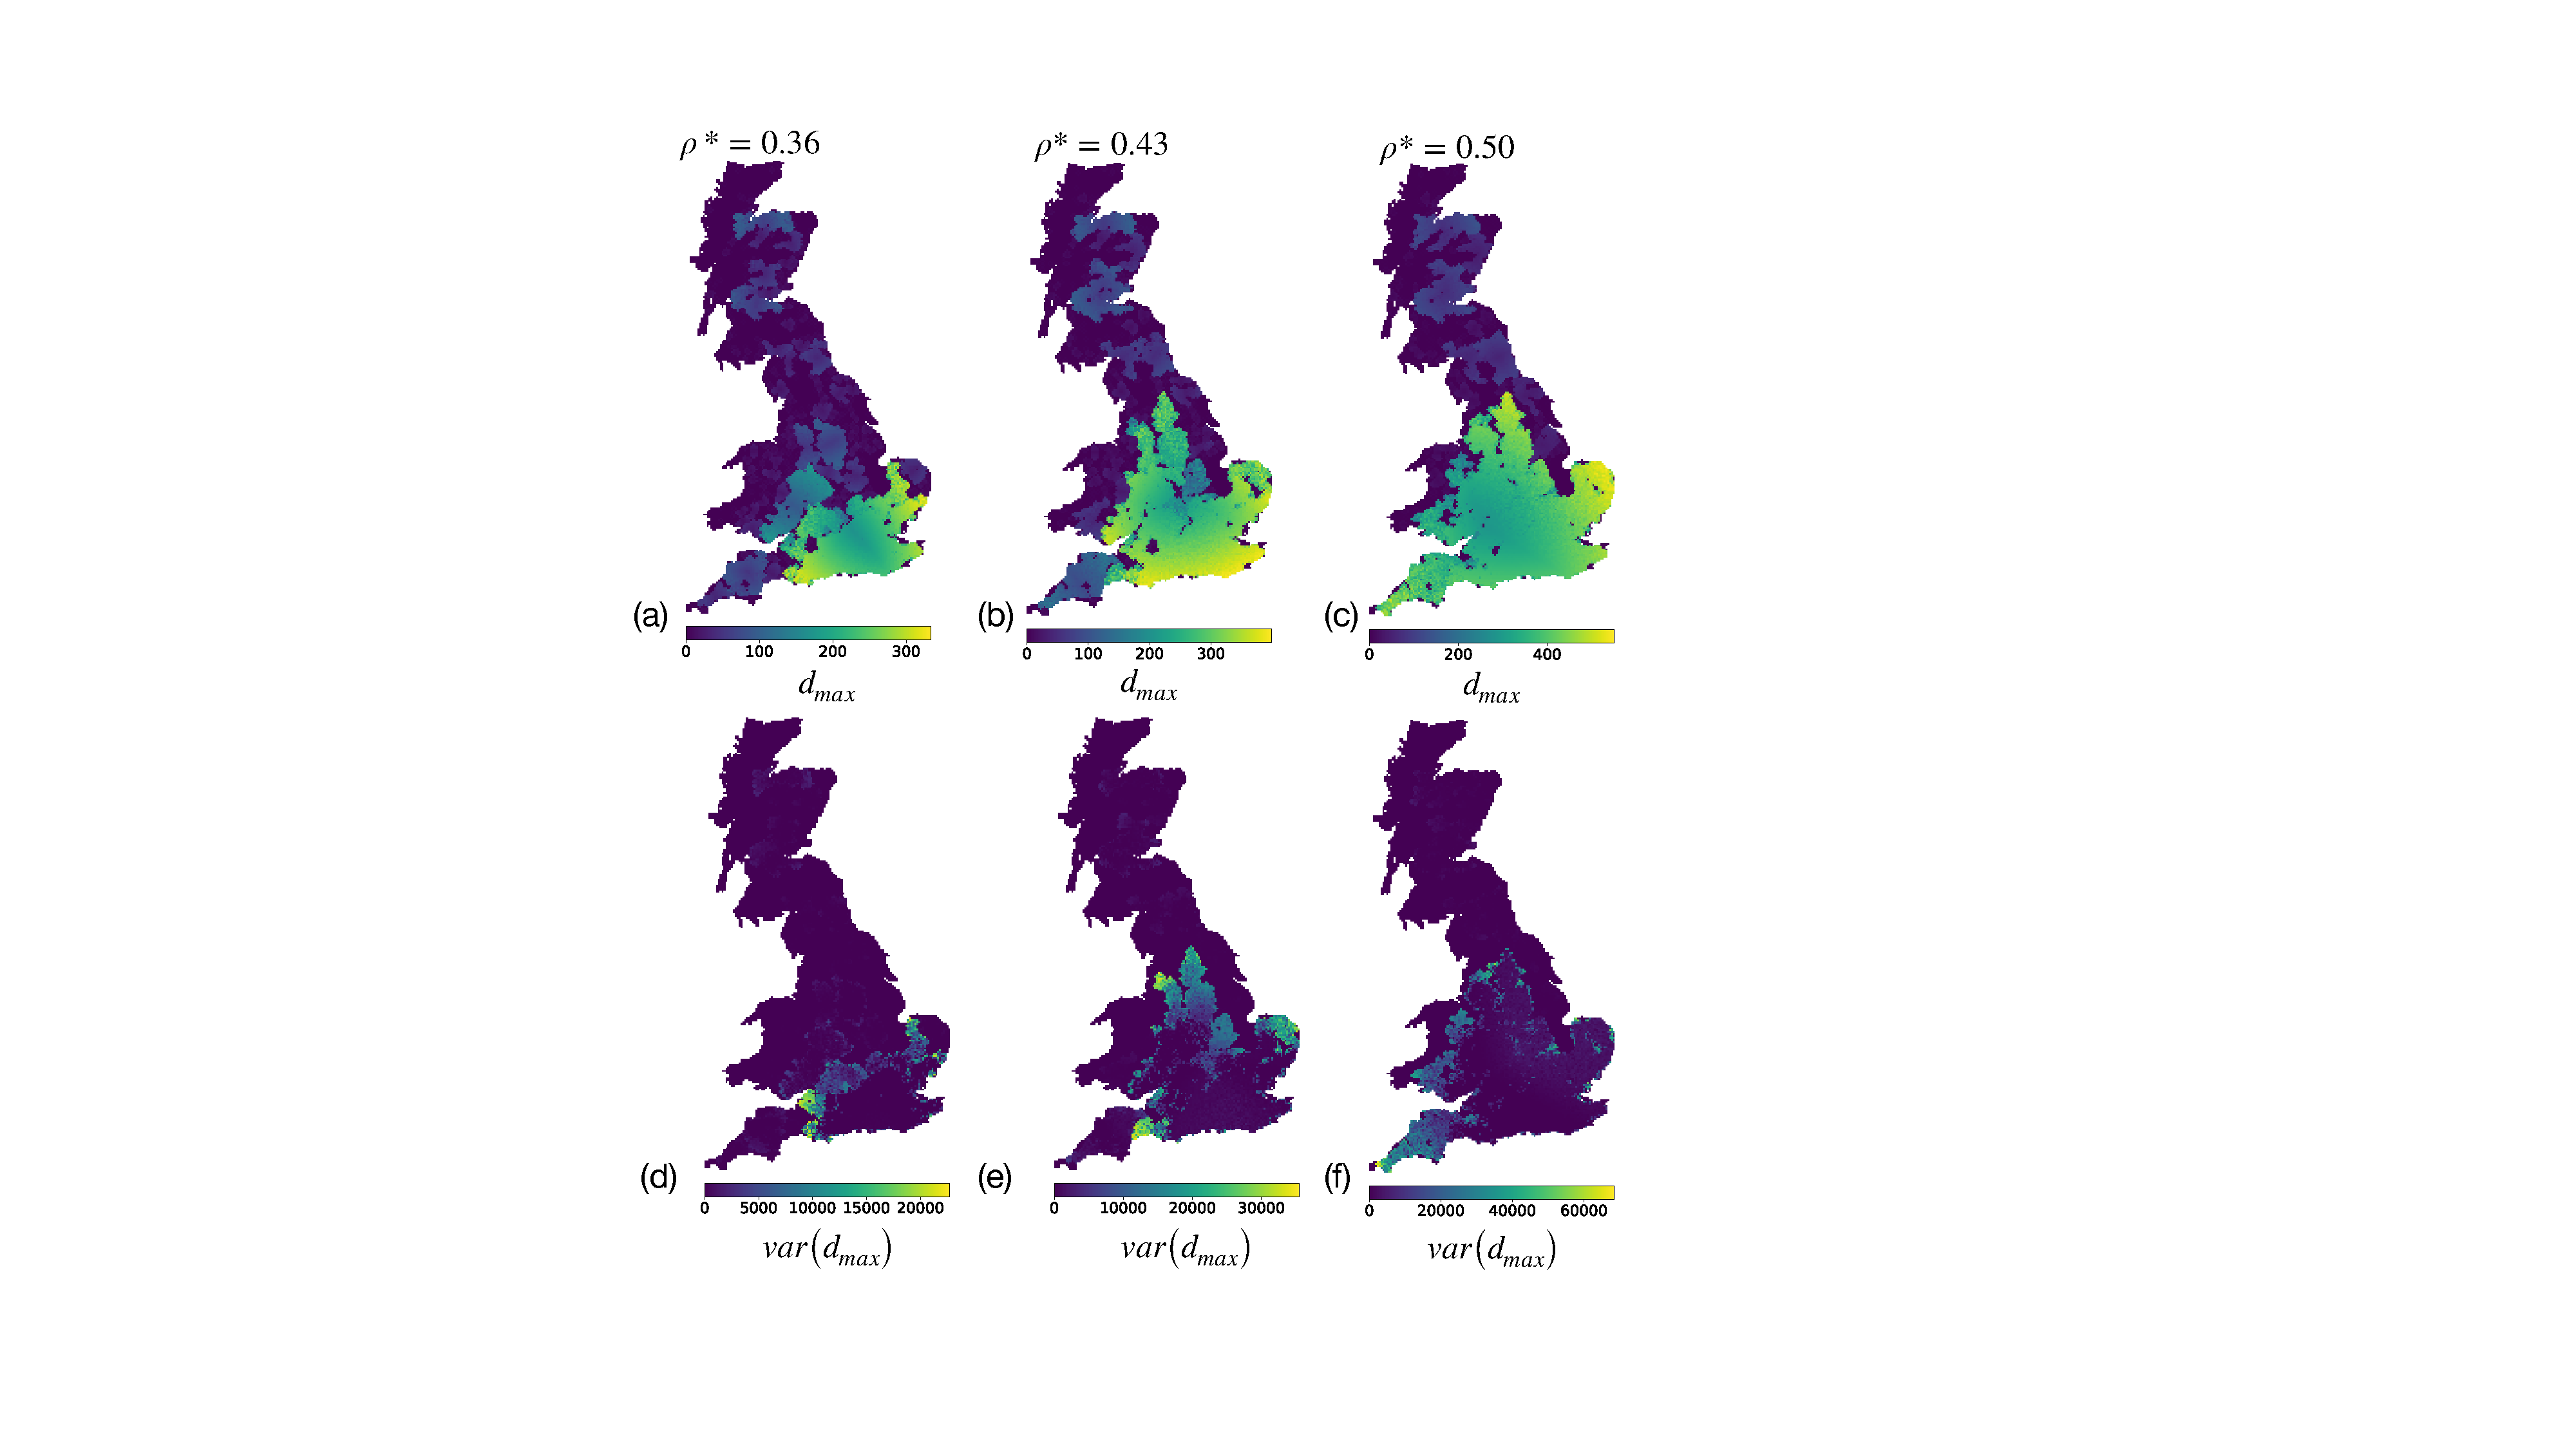
\includegraphics[scale=0.55]{appendix/figures/A-ch4figure1.pdf}
    \caption{The max-distance ($d_{max}$)} metric...
    \label{fig:my_label}
\end{figure}

\chapter{The non-local dispersal model}
\label{section:apendix_A}

\section{An alternate derivation}
\label{eq:alternate-R0}
Starting from an un-normalised Gaussian kernel $g(p, q; \ell) = \exp(\frac{p^2-q^2}{2\ell^2})$ and infectivity constant $\beta$, we may define the probability of position $q$ being infected due to an infected tree at $p$ as $Pr(q; p) = \beta g(p, q; \ell)$. The domain has tree density $\rho_0$ at time $t=0$ and trees transition through states: $S\rightarrow I\rightarrow R$, with $I$ lasting for $T$ time-steps. Considering the probability of point $q = (x, y)$ becoming infected on account of an infected tree located at the origin during the first time-step:
\begin{equation}
    Pr(x, y, t=0) = \beta \rho_0 \exp(-\frac{x^2+y^2}{2\ell^2})
\end{equation}{}
 Integrating this over an infinite domain gives $R_0(t=0)$ expected infections, given by:
\begin{equation}
    R_0(t = 0) = \beta \rho_0 \int^{\infty}_{-\infty} \exp(-\frac{x^2+y^2}{2\ell^2})dx dy= 2\pi\beta\rho_0\ell^2
\end{equation}{}
At time-step $t+1$ there are less trees to infect. Therefore tree density $\rho$ should also be considered as a monotonically decreasing function of time $\rho(t)$, and the number of expected infections should be given by:
\begin{equation}
    R_0(t) = 2\pi\beta\ell^2\rho(t)
    \label{eq:r0-A}
\end{equation}{}
 Considering density as a function of time\footnote{Density also varies with space as trees are removed quicker for regions closer around the primary infection. However, negating this lead to an easily solvable expression valid for lower-value regimes.} in a discrete domain of size $L$, the average decrease in tree density over one time-step is given by:

\begin{equation}
\label{eq:discrete-rho-t-A}
\begin{split}
\rho(t+1) & = \rho(t) - \frac{R_0(t)}{L^2} \\
 & = \rho(t)\Big(1 - 2\pi\beta\frac{\ell^2}{L^2} \Big)
\end{split}
\end{equation}

at $\rho(t=0)=\rho_0$, therefore, equation (\ref{eq:discrete-rho-t-A}) forms a series from which we may expand to give a continuous equation of $\rho$:
\begin{equation}
    \rho(t) = \rho_0 \big(1 - 2\pi\beta\frac{\ell^2}{L^2}\big)^t
\end{equation}{}
upon substitution back into equation (\ref{eq:r0-A}) we have an approximation for how the number of expected infections from one infected tree is expected to change over time:
\begin{equation}
    R_0(t) = 2\pi\beta\ell^2\rho_0 \big(1 - 2\pi\beta\frac{\ell^2}{L^2} \big)^t
    \label{eq:Rt-A}
\end{equation}{}
This expression is compared against numerical simulations in Fig \ref{fig:sgm-evol}(c). Then integrating over the infectious life-time $t=T$ gives an approximation to an effective reproductive number denoted by $R_0$:

\begin{equation} \label{eq1}
\begin{split}
R_0 & = 2\pi\beta\ell^2\rho_0 \int ^T _0 \big(1 - 2\pi\beta\frac{\ell^2}{L^2} \big)^t dt \\
 & = 2\pi\beta\ell^2\rho_0 \frac{ (1 - 2\pi \beta\frac{\ell^2}{L^2})^T - 1}{\ln(1 - 2\pi\beta\frac{\ell^2}{L^2})}
\end{split}
\end{equation}

(from $\int c^t dt = \frac{c^t}{\ln(c)}$). The expression for $R_0$ can be simplified by noting the pathogen is unlikely to infect trees beyond a distance of $3\ell$, therefore, we can replace the area of the domain with the area over three standard deviations (i.e. $9\pi\ell^2$), thus leading to the approximation:
\begin{align*}
    R_0 = 2\pi\beta\rho_0\ell^2 \frac{(1 - 2/9\beta)^T - 1}{\ln(1-2/9\beta)}
\end{align*}

\newpage

\section{SIR fitting}
\label{A:sir-fitting}
\begin{figure}
    \centering
    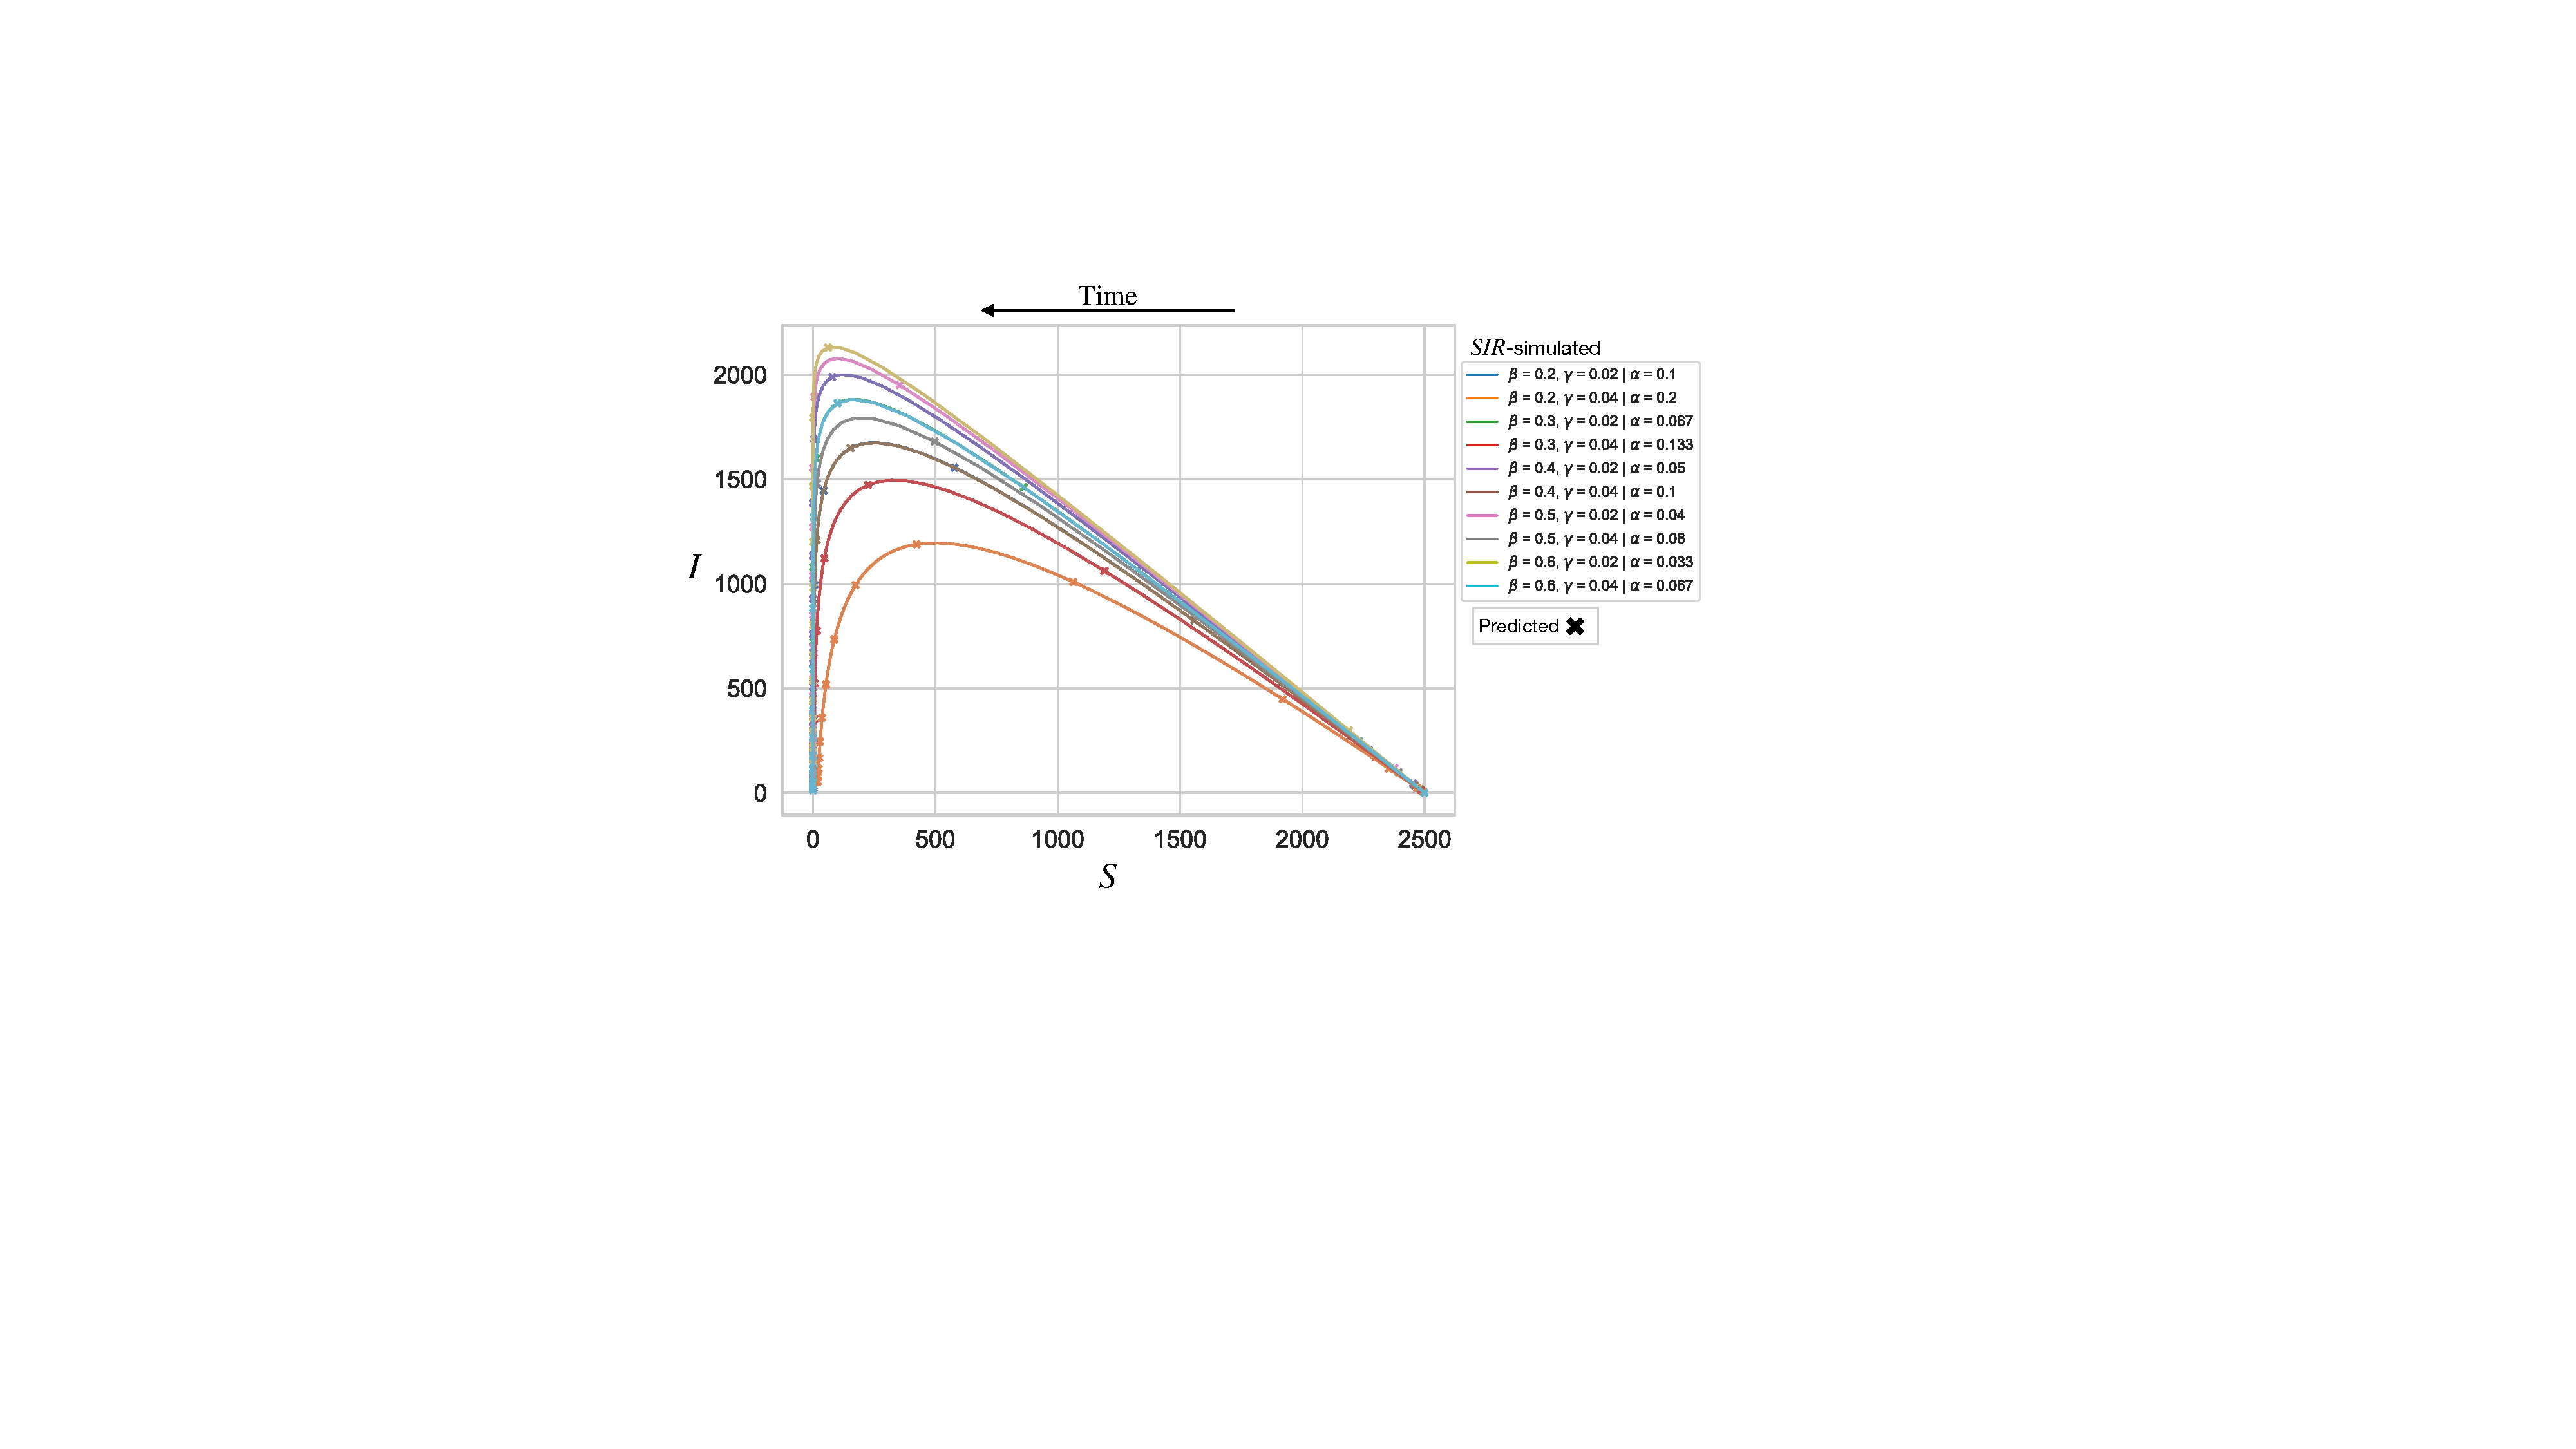
\includegraphics[scale=0.54]{chapter5/figures/fig2-sir-fitting-A.pdf}
    \caption{Infected hosts are plotted as a function hosts, according to the $SIR$ model for various ratios of $\alpha=\gamma / \beta$.
            Initial conditions began from one infected and 2500 susceptible hosts\textemdash equivalent to a $500\times500$ domain at tree density $0.01$.
            Numerical solutions of the $SIR$ model are plotted against predictions from equation \ref{eq:SIR-1param1}, shown as crosses.}
    \label{fig:sir-fitting-a}
\end{figure}

The standard $SIR$ model has no well-known analytic solution, which complicates model fitting.
As such, a simplified scheme that reduced the $SIR$ model to one parameter was used as a comparative tool to access NLM simulations.
Previously in chapter \ref{ch:dispersal-model}, details were omitted about the behaviour of equation \ref{eq:SIR-1param1}, i.e.
\[
I(S) = -S +  N \Big( 1 + \alpha \ln(S / S_0) \Big)
\]
In Figure \ref{fig:sir-fitting-a}, numerical simulations of the $SIR$ model are compared against analytic predictions from equation \ref{eq:SIR-1param1}.
Specifically, the $SIR$ model was simulated\textemdash using the Euler method\textemdash for various combinations of infectivity rate $\beta$ and removal rate $\gamma$ beginning from
one initially infected and 2500 susceptible hosts.
Numerical $SIR$ simulations and predictions of infected hosts $I$ (from equation \ref{eq:SIR-1param1}) are shown as solid lines and crosses respectively.
As the ratio $\alpha=\gamma/\beta$ decreases, a sharper rise in the infections field $I$ results, indicating a more infectious outbreak.
In contrast, a larger value of $\alpha$ defines a smoother curve which attains a lower peak.
Although equation \ref{eq:SIR-1param1} has clear limitations and descriptive power, it allows a simple one-parameter model to fit the NLM against.

\newpage

\section{Exponentially distributed times}

\begin{figure}[h]
    \centering
    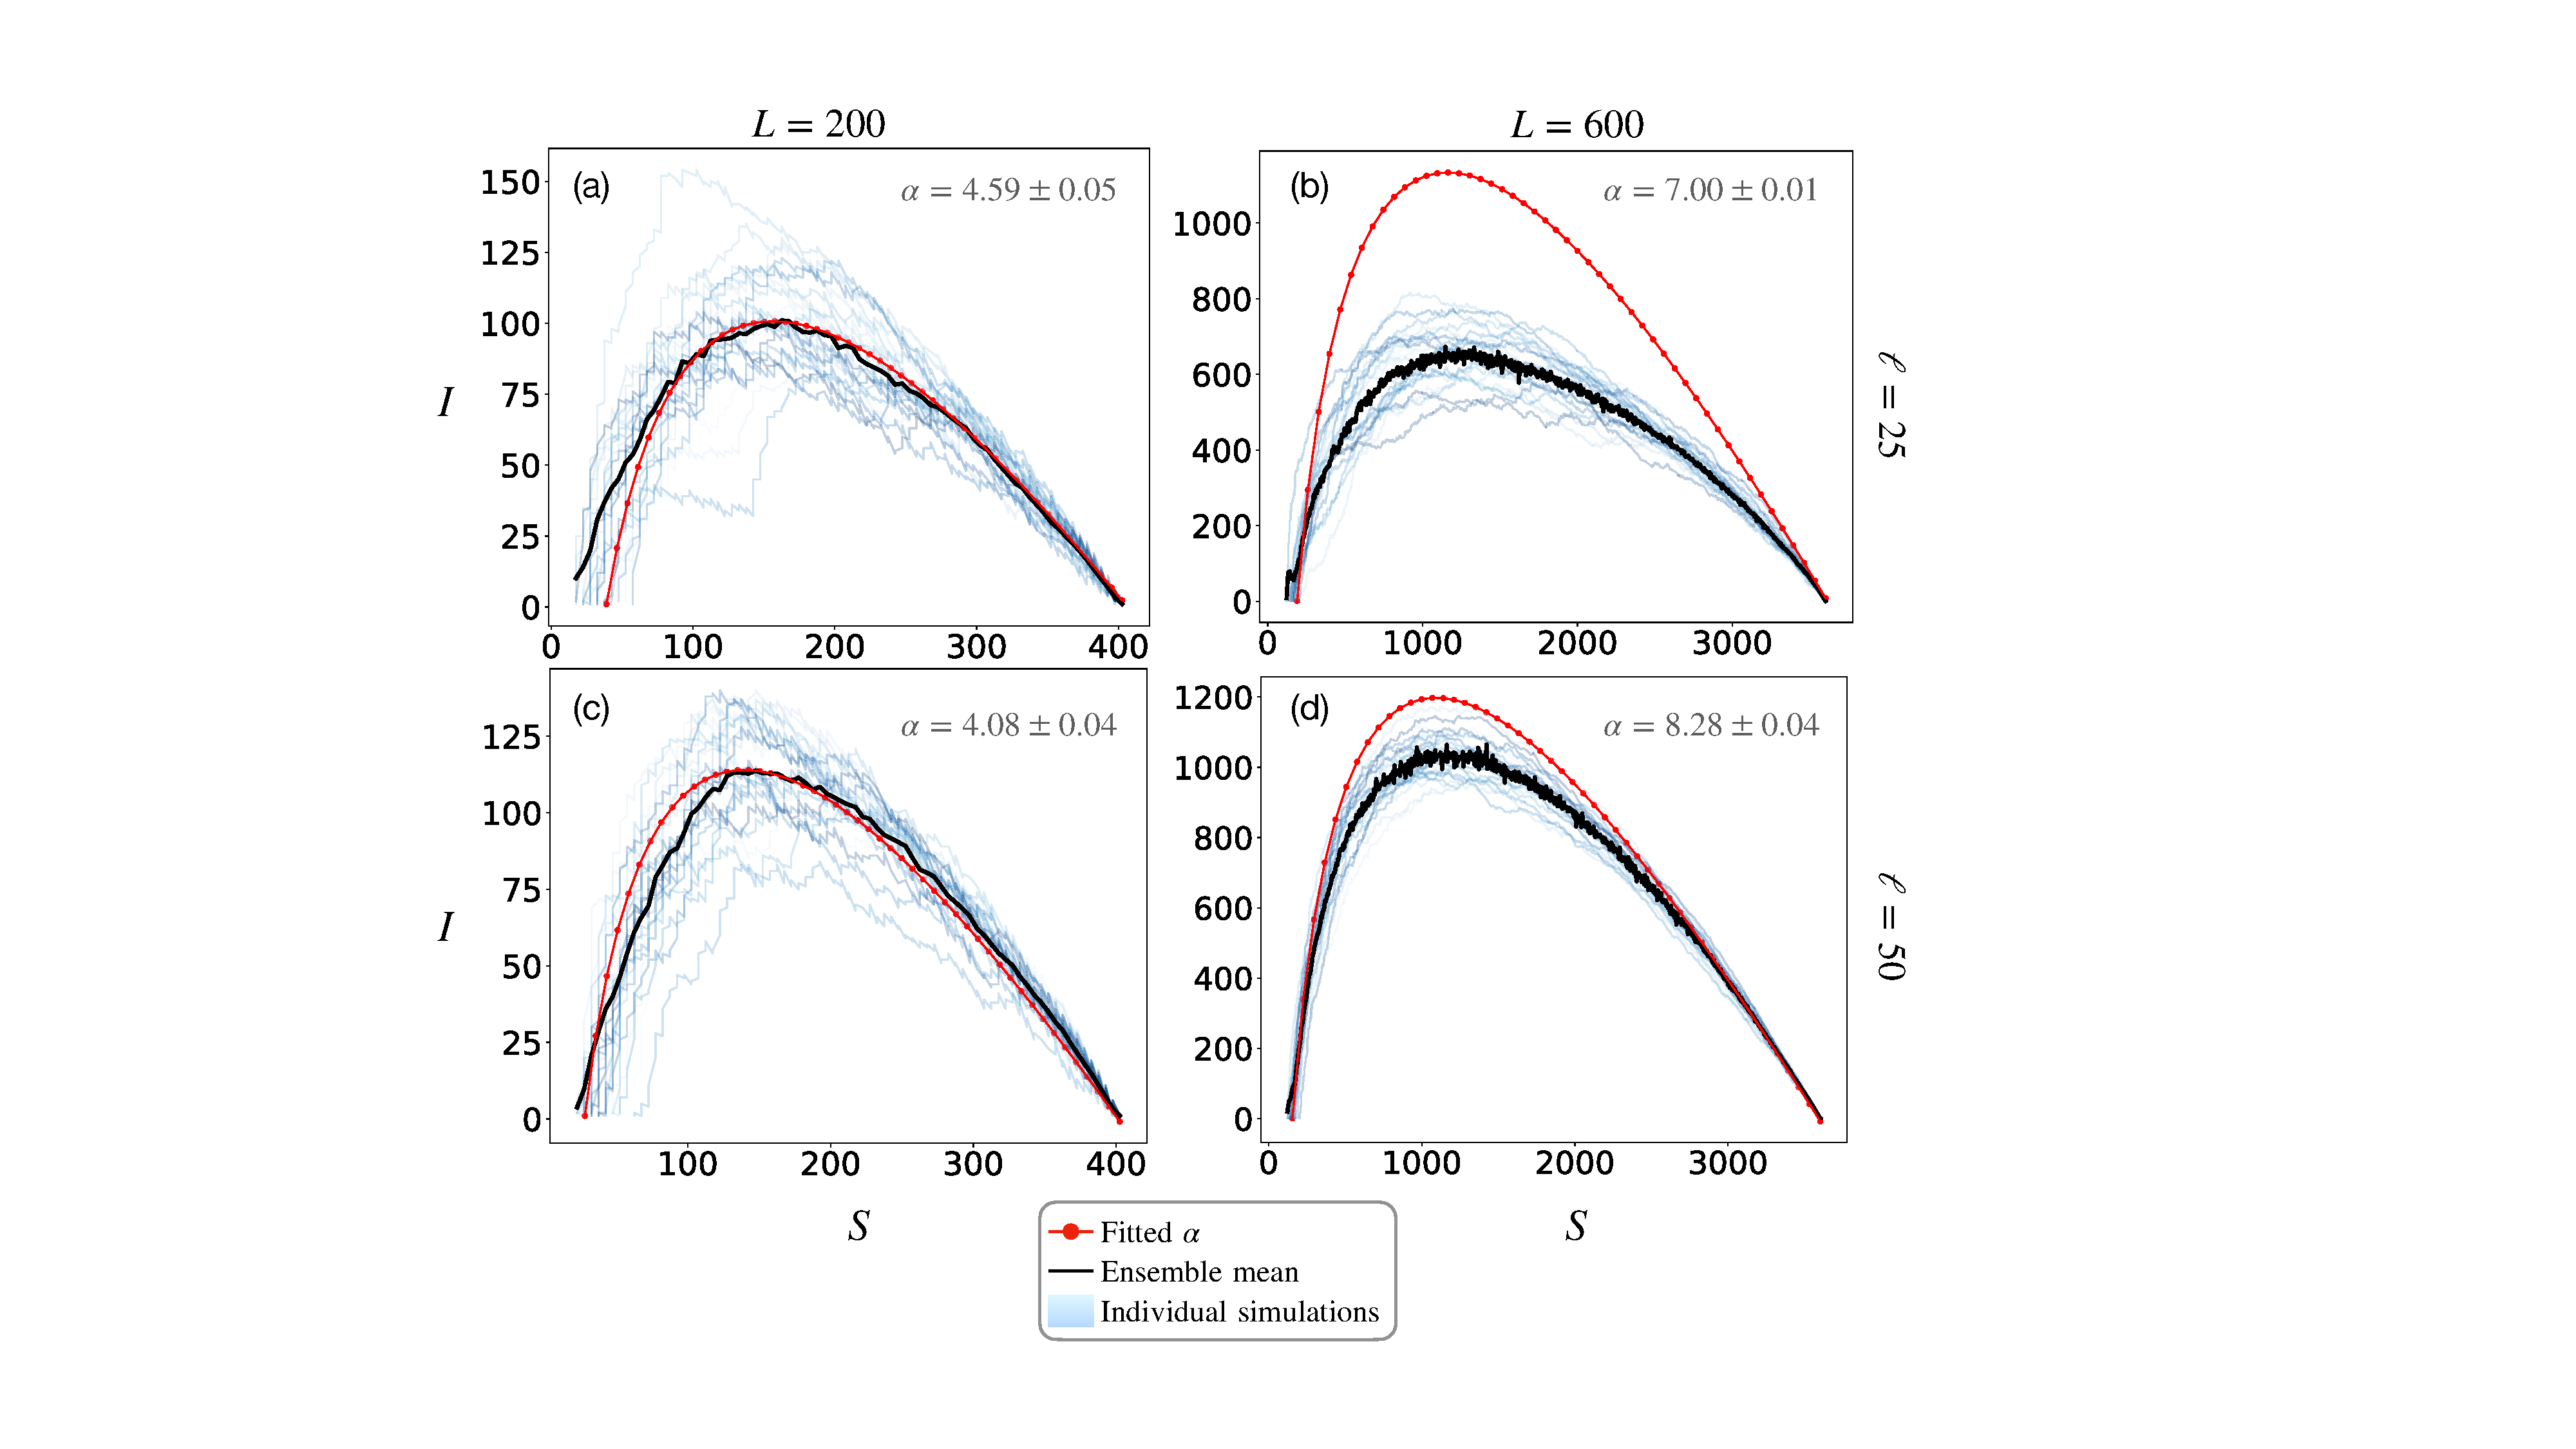
\includegraphics[scale=0.4]{chapter5/figures/fig2-sir-fitting-exp.pdf}
    \caption{Caption}
    \label{fig:SIR-fitting-expontial}
\end{figure}


\label{a:exponentially-distributed-lt}
In chapter 5 the NLM was constructed with uniform transitions into the removed compartment. 
Here, uniform refers to a transition into the $R$ compartment exactly $T$ time-steps after the host becomes infected.
Arguably, uniform life-time transitions are simple and unrealistic.
As such, the NLM constructed in chapter \ref{ch:dispersal-model} was re-run with exponentially-distributed life-times. 
Figure \ref{fig:SIR-fitting-expontial} shows the SIR fitting procedure against the exponentially-distributed variant of the NLM. 
Model behaviour in Figure \ref{fig:SIR-fitting-expontial} looks much the same, although fitting the exponentially-distributed NLM to the SIR model resulted in a closer fit for all panels except (b). 
Figure \ref{fig:SIR-fitting-expontial}(b) shows a much larger disparity between the NLM and SIR model.


\newpage

\section{Combining probabilities in the NLM}
\label{A:combiniing-probabilities}

As mentioned in section \ref{sec:contract-traced-R0}, probabilities in the NLM are simplistic.
That is, we consider interactions between infected and susceptible hosts one by one at each time-step.
In pseudo-code, the essential implementation follows:

\begin{lstlisting}[style=pythoncode,
    caption = ,
    label = py:rand]

def run_algorithm():
    for time_step in range(run_times):  # iterate over time
        for infected_tree in I_arr:  # iterate over I trees
            for susceptible_tree in S_arr:  # iterate over S trees
                Pr(S_x --> I_x ; I_y)
                ...
                ...
                ...
\end{lstlisting}

although these singular between-tree interactions (handled sequentially) are sufficient to model the spread of disease, it would be interesting to compare against a `multi-interaction' implementation by combining probabilities of the form:
\begin{equation}
    Pr(S_x \rightarrow I_{x}; I_{y1}, I_{y2})
\end{equation}
where $I_{y1}$ and $I_{y2}$ are two distinct trees and $y1 \neq y2$.
Now, suppose infection pressure from the two infected trees at location $y1$ and $y2$ simultaneously interact with one susceptible tree at location $x$.
Over a single time-step the combined probability is then:
\begin{equation}
    Pr(S_x \rightarrow I_{x}; I_{y1}, I_{y2}) = P_{y1} + P_{y2} - \big[ P_{y1} \cap P_{yn} \big] 
\end{equation}
where $P_{y1}$ and $P_{y2}$ are the individual probabilities of transition due to $y1$ and $y2$ respectively.
Now, suppose there are $yN$ infected trees, the combined probability is given by the inclusion-exclusion principle:
\begin{equation}
\label{eq:combined-pr}
     Pr(S_x \rightarrow I_{x}; I_{y1}, I_{y2}...I_{yN}) = \sum_{k=1}^{N} \big(  -1 \big)^{k+1} \Big[ \sum _{1\leq y1 \leq y2 \leq....\leq P_{yk} \leq N} \big| P_{y1}\cap ...\cap P_{yk}  \big|   \Big]
\end{equation}

where each union $P_{y1} \cap ... \cap P_{yk}$ adds a small order correction to the original NLM formulation.
It must be remarked how equation \ref{eq:combined-pr} would incur a significant computational cost.
Moreover, because secondary can be induced under the influence of multiple sources the definition of $R_0$ becomes obscure.  
Although implementing equation \ref{eq:combined-pr} would be an interesting\textemdash and potentially insightful\textemdash endeavour, the analysis was not undertaken.

\section{Contact-tracing $R_0$}
\label{A:R0-contact-traced-mortality}

\begin{figure}
    \centering
    \includegraphics[scale=0.60]{chapter5/figures/fig6-R0-contact-vs-mortality-A.pdf}
    \caption{Comparing the contact-traced reproduction ratio against tree mortality. (a) Inverting the plot of Figure \ref{fig:contact-trace-vs-mortality} to show the spread of $R_0^{(1)}$ against the ensemble averaged tree mortality. (b)
    Re-running the ensemble shown in Figure \ref{fig:contact-trace-vs-mortality} with $10$ initially infected trees. The threshold appears more abrupt and stochasticity is reduced.}
    \label{fig:R0-contact-vs-morality-A}
\end{figure}

In Figure \ref{fig:R0-contact-vs-morality-A}(a), we invert the plot (shown in chapter \ref{ch:dispersal-model} Figure \ref{fig:contact-trace-vs-mortality}) and show the range of first generation reproduction ratios $R_0^{(i1)}$ against the ensemble-averaged tree mortality.
Inverting the plot gives information about the spread of $R_0^{(1)}$;
as we can see, low values of infectiviy produce a skewed distribution which becomes more centered as infectivity increases.
A threshold can be seen around $R_0^{(1)}=1$, although a number of simulations can produce a low-valued $R_0^{(1)}$ for any value of infectivity due to initial extinction events.

In chapter \ref{ch:dispersal-model} both the contact and analytic values of $R_0$ were computed/observed for a single infectious tree at the domain center.
As elaborated in chapter \ref{ch:dispersal-model}, initial stochastic forces had the tendency to reduce the chance of epidemic by causing early extinction events\textemdash thereby reducing the mean tree mortality.
However, a number of initial conditions are possible.
As such, the plot of Figure \ref{fig:contact-trace-vs-mortality} was re-run with $10$ infectious trees in the domain center at $t=0$ to test how initial stochasticity in the system changes, shown by Figure \ref{fig:R0-contact-vs-morality-A}(b).

As expected, increasing the number of infected trees at $t=0$ reduces stochastic and early extinction events;
this is demonstrated by noting that Figure \ref{fig:R0-contact-vs-morality-A}(b) has a smoother ensemble mean, and no instances of zero mortality for highly infectious epidemics (c.f. the bottom right hand side of Figure \ref{fig:contact-trace-vs-mortality} where multiple observations can be seen of zero tree mortality for high $\beta^*$).
Surprisingly, for later generations the degree of inflexion for $R_0^{(4)}$-$R_0^{(5)}$ is reduced at high $\beta^*$ in comparison to Figure \ref{fig:contact-trace-vs-mortality},

\newpage


\chapter{Seasonal $SEIR$ model of Ash dieback}

\label{section:ga-SEIR-variant}
\begin{itemize}
    \item The Gaussian and inverse power-law models are distinct and could be considered to have different infecitivity parameters $\beta_{ga}$ and $\beta_{pl}$k.
\end{itemize}

\section{Connected component analysis}

\blindtext

\blindtext


\chapter{Towards landscape-level control}

\blindtext

\blindtext

\begin{figure}
    \centering
    \includegraphics[scale=0.5]{appendix/Graphical_Abstract.pdf}
    \caption{Caption}
    \label{fig:my_label}
\end{figure}






% -----------------------------------------------------------------------------
% Reference list
\bibliographystyle{apalike}. 
% \bibliographystyle{acm}
\bibliography{references}
\end{document}
